\documentclass[10pt,twoside]{thesis}

%!TEX root=tese.tex
\usepackage{amsmath}
\usepackage{amssymb}
\usepackage[utf8]{inputenc}
\usepackage[T1]{fontenc}
\usepackage[portuguese]{babel}
\usepackage[utopia]{mathdesign}
\usepackage[scaled]{beramono}
\usepackage[a4paper,left=3.5cm,right=2.5cm,top=2.5cm,bottom=2.5cm]{geometry}
\usepackage{aecompl}
\usepackage[center,nooneline,font={footnotesize}]{caption}
\usepackage[pdftex]{graphicx}
\usepackage{attachfile2}                                    
\usepackage{hyperref}
\usepackage{xcolor}
\usepackage[squaren,thinspace,textstyle]{SIunits}
\usepackage[version=3]{mhchem}
\usepackage{breqn}
\usepackage{fancyvrb}
\usepackage{booktabs}
\usepackage{dcolumn}
\usepackage{threeparttable}
\usepackage{multirow}
\usepackage{tikz}
\usepackage{pgfplots}
\usepackage{rotating}
\usepackage{fancyhdr}
\usepackage{colortbl}
\usepackage{multirow}
\usepackage{diagbox}
\usepackage{algorithm}
\usepackage[noend]{algorithmic}
\usepackage{etoolbox}
\usepackage{setspace}
\usepackage{tabularx}
\usepackage{makeidx}
\usepackage[notintoc,portuguese]{nomentblze}
\usepackage{listings} 
\usepackage{lipsum}
\usepackage{upquote}
\usepackage{amsthm}

\DeclareGraphicsExtensions{.jpg,.png}
\graphicspath{{.}{images/}}
\definecolor{linkcol}{rgb}{0,0,0}
\definecolor{citecol}{rgb}{0,0,0}

%%%% Definidos por mim %%%%
\providecommand{\mc}[3]{\multicolumn{#1}{#2}{#3}}
\providecommand{\mr}[1]{\mathrm{#1}}
\providecommand{\tce}[1]{$\ce{#1}$}
\providecommand{\pCAMBIA}{\emph{pCAMBIA-1303}}
\providecommand{\et}{et al}
\providecommand{\fluxocritico}{\ensuremath{J_{\mathrm{crit}}}}
\providecommand{\fluxo}{\ensuremath{J_{\mathrm{V}}}}
\providecommand{\fluxosoluto}{\ensuremath{J}}
\providecommand{\kapace}{\ensuremath{K_{\mathrm{c}}}}
\providecommand{\kapade}{\ensuremath{K_{\mathrm{d}}}}
\providecommand{\cargamembrana}{\ensuremath{Q_{x}}}
\providecommand{\porcento}{\,\%}
\providecommand{\molar}{\,M}
\providecommand{\kpb}{\ensuremath{\,\mathrm{kbp}}}
\providecommand{\kilopb}{\ensuremath{\mathrm{kbp}}}
\providecommand{\npb}{\ensuremath{\,\mathit{nbp}}}
\providecommand{\numpb}{\ensuremath{\mathrm{nbp}}}
\providecommand{\milimolar}{\ensuremath{\mathrm{\,mM}}}
\providecommand{\deborahcritico}{\ensuremath{\mathrm{De}_{\mathrm{crit}}}}
\providecommand{\deborah}{\ensuremath{\mathrm{De}}}
\providecommand{\permeacaoobservada}{\ensuremath{S_{obs}}}
\providecommand{\boltzman}{\ensuremath{k_{\mr{B}}}}
\providecommand{\raioporo}{\ensuremath{r_{\mr{p}}}}
\providecommand{\viscosidade}{\ensuremath{\eta}}
\providecommand{\raiogiracao}{\ensuremath{r_{\mr{g}}}}
\providecommand{\raiogiracaoinst}{\ensuremath{\raiogiracao^{*}}}
\providecommand{\raiostokes}{\ensuremath{r_{\mr{s}}}}
\providecommand{\raiosuperhelice}{\ensuremath{r_{H}}}
\providecommand{\dinf}{\ensuremath{D_{\mathit{\infty}}}}
\providecommand{\coeficientemassa}{\ensuremath{k}}
\providecommand{\avogadro}{\ensuremath{N_{A}}}
\providecommand{\reynolds}{\ensuremath{\mathrm{Re}}}
\providecommand{\particao}{\ensuremath{\Phi}}
\providecommand{\lambdah}{\ensuremath{\lambda_{\mr{h}}}}
\providecommand{\lambdas}{\ensuremath{\lambda_{\mr{s}}}}
\providecommand{\lambdag}{\ensuremath{\lambda_{\mr{g}}}}
\providecommand{\distanciah}{\ensuremath{\left\langle h^{2}\right\rangle^{1/2}}}
\providecommand{\lambdahfor}{\ensuremath{\distanciah\!\!/\raioporo}}
\providecommand{\concentracao}{\ensuremath{C}}
\providecommand{\concp}{\ensuremath{C_{\mathrm{p}}}}
\providecommand{\concb}{\ensuremath{C_{\mathrm{b}}}}
\providecommand{\concm}{\ensuremath{C_{\mathrm{m}}}}
\providecommand{\permm}{\ensuremath{S_{\mathrm{m}}}}
\providecommand{\permobs}{\ensuremath{S_{\mathrm{obs}}}}
\providecommand{\concpi}{\ensuremath{C_{\mathrm{p,i}}}}
\providecommand{\concbi}{\ensuremath{C_{\mathrm{b,i}}}}
\providecommand{\concmi}{\ensuremath{C_{\mathrm{m,i}}}}
\providecommand{\concMi}{\ensuremath{C_{\mathrm{M,i}}}}
\providecommand{\permmi}{\ensuremath{S_{\mathrm{m,i}}}}
\providecommand{\permobsi}{\ensuremath{S_{\mathrm{obs,i}}}}
\providecommand{\perminf}{\ensuremath{S_{\infty}}}
\providecommand{\permmum}{\ensuremath{S_{\mathrm{m,1}}}}
\providecommand{\permmdois}{\ensuremath{S_{\mathrm{m,2}}}}
\providecommand{\permmtres}{\ensuremath{S_{\mathrm{m,3}}}}
\providecommand{\permobsum}{\ensuremath{S_{\mathrm{obs,1}}}}
\providecommand{\permobsdois}{\ensuremath{S_{\mathrm{obs,2}}}}
\providecommand{\permobstres}{\ensuremath{S_{\mathrm{obs,3}}}}
\providecommand{\concmum}{\ensuremath{C_{\mathrm{m,1}}}}
\providecommand{\concMum}{\ensuremath{C_{\mathrm{M,1}}}}
\providecommand{\concmdois}{\ensuremath{C_{\mathrm{m,2}}}}
\providecommand{\concMdois}{\ensuremath{C_{\mathrm{M,2}}}}
\providecommand{\concmtres}{\ensuremath{C_{\mathrm{m,3}}}}
\providecommand{\concMtres}{\ensuremath{C_{\mathrm{M,3}}}}
\providecommand{\concbum}{\ensuremath{C_{\mathrm{b,1}}}}
\providecommand{\concbdois}{\ensuremath{C_{\mathrm{b,2}}}}
\providecommand{\concbtres}{\ensuremath{C_{\mathrm{b,3}}}}
\providecommand{\concpum}{\ensuremath{C_{\mathrm{p,1}}}}
\providecommand{\concpdois}{\ensuremath{C_{\mathrm{p,2}}}}
\providecommand{\concptres}{\ensuremath{C_{\mathrm{p,3}}}}
\providecommand{\numsegmento}{\ensuremath{n_{k}}}
\providecommand{\comsegmento}{\ensuremath{l_{k}}}
\providecommand{\registado}{\textsuperscript{\textregistered}}
\providecommand{\vectorpos}{\ensuremath{\vec{r}_{i}}}
\providecommand{\vectorcm}{\ensuremath{\vec{r}_{\mathrm{cm}}}}
\providecommand{\contorno}{\ensuremath{L}}
\providecommand{\kuhn}{\ensuremath{l_{K}}}
\providecommand{\persis}{\ensuremath{a}}
\providecommand{\forcaionica}{\ensuremath{I}}
\providecommand{\inversodebye}{\ensuremath{\kappa}}
\providecommand{\raioduplahelice}{\ensuremath{R_{\mathrm{DNA}}}}
\providecommand{\cargaeletrica}{\ensuremath{z}}
\providecommand{\bjerrum}{\ensuremath{l_{B}}}
\providecommand{\densidadecarga}{\ensuremath{\xi}}
\providecommand{\numeroeuler}{\ensuremath{\mathrm{e}}}
\providecommand{\contornosuper}{\ensuremath{L_{s}}}
\providecommand{\persissuper}{\ensuremath{a_{s}}}
\providecommand{\agitacao}{\ensuremath{\omega}}
\providecommand{\densidade}{\ensuremath{\rho}}
\providecommand{\fracaomembrana}{\ensuremath{\theta}}
\providecommand{\ctefaraday}{\ensuremath{F}}
\providecommand{\ctegases}{\ensuremath{R}}
\providecommand{\potencial}{\ensuremath{\Psi}}
\providecommand{\atividade}{\ensuremath{a}}
\providecommand{\potencialD}{\ensuremath{\Delta\Psi_{D}}}
\providecommand{\Nadsorvido}{\ensuremath{N_{\mathrm{ads}}}}
\providecommand{\potencialgrad}{\ensuremath{(d\Psi/dy)_{\mr{m}}}}
\providecommand{\comporo}{\ensuremath{L}}
\providecommand{\velocidadesolvente}{\ensuremath{v}}
\providecommand{\velocidadesoluto}{\ensuremath{u}}
\providecommand{\radialadimensional}{\ensuremath{\beta}}
\providecommand{\massamolecular}{\ensuremath{M_\mathrm{w}}}
\providecommand{\daltons}{\ensuremath{\mathrm{Da}}}
\providecommand{\raiocelula}{\ensuremath{r_{\mathrm{cell}}}}
\providecommand{\minmum}{\ensuremath{\mathrm{min^{-1}}}}
\providecommand{\atrito}{\ensuremath{\zeta}}
\providecommand{\potqui}{\ensuremath{\mu}}
\providecommand{\fluxoporo}{\ensuremath{j_{\mathrm{V}}}}
\providecommand{\caudal}{\ensuremath{Q}}
\providecommand{\numporo}{\ensuremath{n_{p}}}
\providecommand{\areamembrana}{\ensuremath{A_{\mathrm{m}}}}
\providecommand{\porosidade}{\ensuremath{\varepsilon}}
\providecommand{\tortuosidade}{\ensuremath{\tau}}
\providecommand{\commembrana}{\ensuremath{L_{\mathrm{m}}}}
\providecommand{\permhidra}{\ensuremath{L_{\mathrm{p}}}}
\providecommand{\potencialms}{\ensuremath{\Upsilon}}
\providecommand{\conctotal}{\ensuremath{C_{\mathrm{T}}}}
\providecommand{\peclet}{\ensuremath{\mathrm{Pe}}}
\providecommand{\euler}{\ensuremath{\mathrm{e}}}
\providecommand{\volumeparcial}{\ensuremath{V_{\mathrm{s}}}}
\providecommand{\sedimentacao}{\ensuremath{s}}
\providecommand{\sulfatoamonio}{\ensuremath{\mathrm{(NH_{4})_{2}SO_{4}}}}
\providecommand{\volumeparcial}{\ensuremath{V_{\mathrm{s}}}}
\providecommand{\sedimentacao}{\ensuremath{s}}
\providecommand{\remocaoum}{\ensuremath{R_{1}}}
\providecommand{\remocaodois}{\ensuremath{R_{2}}}
\providecommand{\cacldois}{\ensuremath{\mathrm{CaCl_{2}}}}
\providecommand{\volretencao}{\ensuremath{V_{\mathrm{R}}}}
\providecommand{\fjc}{cadeias de ligação livre}
\providecommand{\Fjc}{Cadeias de rotação livre}
\providecommand{\closedsc}{cadeias segmentadas fechadas}
\providecommand{\Closedsc}{Cadeias segmentadas fechadas}
\providecommand{\wlc}{cadeias ``worm-like''}
\providecommand{\Wlc}{Cadeias ``worm-like''}
\providecommand{\superenrolada}{super-enrolada}
\providecommand{\pVAX}{\emph{pVAX1-LacZ}}
\providecommand{\pUC}{\emph{pUC19}}
\providecommand{\ecoli}{\emph{E.\ coli}}
\providecommand{\ecolidh}{\emph{E.\ coli DH5$\alpha$}}
\providecommand{\tracketched}{``track-etched''}
\providecommand{\eppendorf}{Eppendorf}
\providecommand{\espectrofotometro}{espectrofotómetro}
\providecommand{\Espectrofotometro}{Espectrofotómetro}

% TIKZ
\usetikzlibrary{plotmarks}
\usetikzlibrary{patterns}
\pgfplotsset{x tick label style={/pgf/number format/fixed}} 
\pgfplotsset{y tick label style={/pgf/number format/fixed}} 
\newlength{\hatchspread}
\newlength{\hatchthickness}
\newlength{\hatchshift}
\newcommand{\hatchcolor}{}
\tikzset{hatchspread/.code={\setlength{\hatchspread}{#1}},
         hatchthickness/.code={\setlength{\hatchthickness}{#1}},
         hatchshift/.code={\setlength{\hatchshift}{#1}},% must be >= 0
         hatchcolor/.code={\renewcommand{\hatchcolor}{#1}}}
\tikzset{hatchspread=3pt,
         hatchthickness=0.4pt,
         hatchshift=0pt,% must be >= 0
         hatchcolor=black}
\pgfdeclarepatternformonly[\hatchspread,\hatchthickness,\hatchshift,\hatchcolor]% variables
   {custom north west lines}% name
   {\pgfqpoint{\dimexpr-2\hatchthickness}{\dimexpr-2\hatchthickness}}% lower left corner
   {\pgfqpoint{\dimexpr\hatchspread+2\hatchthickness}{\dimexpr\hatchspread+2\hatchthickness}}% upper right corner
   {\pgfqpoint{\dimexpr\hatchspread}{\dimexpr\hatchspread}}% tile size
   {% shape description
    \pgfsetlinewidth{\hatchthickness}
    \pgfpathmoveto{\pgfqpoint{0pt}{\dimexpr\hatchspread+\hatchshift}}
    \pgfpathlineto{\pgfqpoint{\dimexpr\hatchspread+0.15pt+\hatchshift}{-0.15pt}}
    \ifdim \hatchshift > 0pt
      \pgfpathmoveto{\pgfqpoint{0pt}{\hatchshift}}
      \pgfpathlineto{\pgfqpoint{\dimexpr0.15pt+\hatchshift}{-0.15pt}}
    \fi
    \pgfsetstrokecolor{\hatchcolor}
    \pgfusepath{stroke}
   }

\usetikzlibrary{shadows}
\usetikzlibrary{arrows}
\usetikzlibrary{patterns}
\usetikzlibrary{decorations}
\usepgflibrary{decorations.pathreplacing}
\pgfdeclarelayer{background}
\pgfdeclarelayer{foreground}
\pgfsetlayers{background,main,foreground}

\hypersetup
{
pagebackref,
hyperindex=true,
bookmarksopen=true,
pdftitle="Tese",
pdfauthor="J. Nunes",
pdfsubject="Tese",
pdfmenubar=true,
pdfhighlight=/O,
colorlinks=true,
pdfpagemode=UseNone,
pdfpagelayout=SinglePage,
pdffitwindow=true,
linkcolor=linkcol,
citecolor=citecol,
urlcolor=linkcol
}

% Settings
\setcounter{secnumdepth}{3}
\setcounter{tocdepth}{2}

\newcommand{\pd}[2]{\frac{\partial #1}{\partial #2}}
\def\abs{\operatorname{abs}}
\def\argmax{\operatornamewithlimits{arg\,max}}
\def\argmin{\operatornamewithlimits{arg\,min}}
\def\diag{\operatorname{Diag}}
\newcommand{\eqRef}[1]{(\ref{#1})}

% Header and footer
\pagestyle{fancy}
\fancyfoot{}
\fancyhead{}
\fancyfoot[LE,RO]{\thepage}
\newcommand{\cabecalho}[1]{\fancyhead[RE,LO]{\bfseries{#1}}}
\let\headruleORIG\headrule
\renewcommand{\headrule}{\color{black} \headruleORIG}
\renewcommand{\headrulewidth}{0pt}

% Fonts
\newcommand{\capitulos}{\fontsize{22pt}{10pt}\bfseries\selectfont}
\newcommand{\titulos}{\fontsize{18pt}{10pt}\bfseries\selectfont}
\newcommand{\seccao}{\fontsize{14pt}{20pt}\bfseries\selectfont}
\newcommand{\subseccao}{\fontsize{12pt}{14pt}\selectfont}
\renewcommand{\footnotesize}{\fontsize{9pt}{12pt}\selectfont}
\renewcommand{\Huge}{\titulos}

% Cover
\newcommand{\rostoubi}{\fontsize{14pt}{14pt}\selectfont}
\newcommand{\rostotitulo}{\fontsize{18pt}{18pt}\selectfont}
\newcommand{\rostosubtit}{\fontsize{16pt}{16pt}\selectfont}
\newcommand{\rostonomes}{\fontsize{14pt}{14pt}\selectfont}
\newcommand{\rostooutros}{\fontsize{12pt}{12pt}\selectfont}
\newcommand{\rostofac}{\fontsize{12.5pt}{12.5pt}\selectfont}

\addto\captionsportuguese{\renewcommand*{\contentsname}{Índice}}
\addto\captionsportuguese{\renewcommand*{\indexname}{Índice Remissivo}}

\arrayrulecolor{black}

% Page style plain
\fancypagestyle{plain}{
  \renewcommand{\headrulewidth}{0pt}
}


% Blank pages must be numbered
\makeatletter

\def\cleardoublepage{\clearpage\if@twoside \ifodd\c@page\else%
  \hbox{}%
  \thispagestyle{plain}%
  \newpage%
  \if@twocolumn\hbox{}\newpage\fi\fi\fi}

\makeatother

\AtBeginEnvironment{tabular}{\footnotesize}

% Equation number centered
\makeatletter
\def\place@tag{\quad\boxz@}
\makeatother
\let\equation\align
\let\endequation\endalign

\newenvironment{maxime}[1]
{
\vspace*{0cm}
\hfill
\begin{minipage}{0.5\textwidth}%
\hrulefill $\:$ {\bf #1}\\
\it 
}%
{%
\hrulefill
\vspace*{0.5cm}%
\end{minipage}
}

\newenvironment{bulletList}%
{ \begin{list}%
  {$\bullet$}%
  {\setlength{\labelwidth}{25pt}%
   \setlength{\leftmargin}{30pt}%
   \setlength{\itemsep}{\parsep}}}%
{ \end{list} }

\newtheorem{definition}{Définition}
\renewcommand{\epsilon}{\varepsilon}

% Centered page environment
\newenvironment{vcenterpage}
{\newpage\vspace*{\fill}\renewcommand{\headrulewidth}{0pt}}
{\vspace*{\fill}\par\pagebreak}
\newcolumntype{Y}{>{\raggedright\arraybackslash}X}

% Listings style
\definecolor{keycordois}{RGB}{38,139,210}
\definecolor{keycortres}{RGB}{38,139,210}
\definecolor{comcor}{RGB}{147,161,161}
\definecolor{strcor}{RGB}{42,161,152}
\definecolor{ncor}{RGB}{101,123,131}
\definecolor{backcor}{RGB}{253,246,227}
\definecolor{keycor}{RGB}{133,153,0}

\lstdefinelanguage{matlabfloz}{%
  alsoletter={...},%
  morekeywords={%                       % keywords
  break,case,catch,continue,elseif,else,end,for,function,global,%
  if,otherwise,persistent,return,switch,try,while,...},%
  keywords=[2]{np_4c,np_pdna_3c,mantexpnt,fiflex,mem_rp,dpdnapra,%
  iscres,kamicon8010,kc_dech,kd_dech,manning,nernst3c,nernst4c,np_rna_3c,%
  peclet,propRNA,propSAL,rgcsc,rk4arg,sm_hindered,sm2sobs,%
  stokes_einstein,testODE_3c,testODE_4c,visc,sobs_hs,sobs_flex},
  %keywords=[3]{\n},
  comment=[l]\%,%                       % comments
  morecomment=[l]...,%                  % comments
  morestring=[m]',%                       % strings 
}[keywords,comments,strings]%

% Listings package
\lstset{%
basicstyle=\color{ncor}\footnotesize\ttfamily,
language=matlabfloz,
deletekeywords={cond,expo},
numberstyle=\tiny,
numbersep=5pt,
tabsize=2,
extendedchars=true,
breaklines=true,
keywordstyle=[1]\color{keycor},
frame=b,
commentstyle=\color{comcor},         
keywordstyle={[2]\color{keycordois}},
%keywordstyle={[3]\color{keycortres}},
stringstyle=\color{strcor}\ttfamily,
showspaces=false,
showtabs=false,
xleftmargin=17pt,
framexleftmargin=17pt,
framexrightmargin=5pt,
framexbottommargin=4pt,
backgroundcolor=\color{backcor},
showstringspaces=false
}
% Listings legend name
\renewcommand{\lstlistingname}{Função}
% Listings legend
\DeclareCaptionFont{white}{\color{white}}
\DeclareCaptionFormat{listing}{\colorbox[cmyk]{0.43, 0.35, 0.35,0.01}{\parbox{\textwidth}{\hspace{15pt}#1#2#3}}}
\captionsetup[lstlisting]{format=listing,labelfont=white,textfont=white, singlelinecheck=false, margin=0pt, font={bf,footnotesize}}
\newcolumntype{d}[1]{D{,}{.}{#1}}
\newcolumntype{z}[1]{D{?}{\,\pm\,}{#1}}
\theoremstyle{definition}
\newtheorem{rotina}{Rotina}[chapter]
\newlength\figureheight 
\newlength\figurewidth 
\hyphenation{bio-mo-lé-cu-la a-dmi-nis-trar se-gmen-tos}
\widowpenalty=10000
\clubpenalty=10000
\makeindex
\makenomenclature
\cabecalho{Purificação de DNA plasmídico usando tecnologias de membrana}

\begin{document}

%!TEX root=tese.tex
\nomenclature[aSy]{$S_y$}{função de mínimos quadrados}{}%
\nomenclature[aSy]{$V_{\mr{s}}$}{volume parcial específico}{m}%
\nomenclature[aa]{\atividade}{atividade}{}%
\nomenclature[aa]{\persis}{comprimento de persistência}{m}%
\nomenclature[aAm]{\areamembrana}{área de membrana}{m$^2$}%
\nomenclature[aC]{\concentracao}{concentração molar}{mol/m$^3$}%
\nomenclature[aCb]{\concb}{concentração no seio da solução a filtrar}{mol/m$^3$}%
\nomenclature[aCm]{\concm}{concentração junto à superfície da membrana}{mol/m$^3$}%
\nomenclature[aCp]{\concp}{concentração no permeado}{mol/m$^3$}%
\nomenclature[aCT]{\conctotal}{concentração total de uma solução}{mol/m$^3$}%
\nomenclature[aD1]{$D$}{coeficiente de difusão}{m$^2$/s}%
\nomenclature[aDe]{\deborah}{número de Deborah}{}%
\nomenclature[aDec]{\deborahcritico}{número de Deborah crítico}{}%
\nomenclature[aD2]{\dinf}{coeficiente de difusão numa solução não confinada}{m$^2$/s}%
\nomenclature[aF]{\ctefaraday}{constante de Faraday}{$96\,485$\,C/mol}%
\nomenclature[ahq]{\distanciah}{distância média entre as extremidades de uma cadeia FJC}{m}%
\nomenclature[aI]{\forcaionica}{força iónica}{mol/m$^3$}%
\nomenclature[aJ]{\fluxosoluto}{fluxo difusivo}{m/s}%
\nomenclature[aJc]{\fluxocritico}{fluxo crítico}{m/s}%
\nomenclature[ajV]{\fluxoporo}{fluxo volumétrico de solvente num poro}{m/s}%
\nomenclature[aJv]{\fluxo}{fluxo de filtração ou fluxo de permeado}{m/s}%
\nomenclature[ak]{\coeficientemassa}{coeficiente de transferência de massa}{m/s}%
\nomenclature[akB]{\boltzman}{constante de Boltzmann}{$1.381\times 10^{-23}$\,J/K}%
\nomenclature[aKc]{\kapace}{fator de impedimento convectivo}{}%
\nomenclature[aKd]{\kapade}{fator de impedimento difusivo}{}%
\nomenclature[aL]{\comporo}{comprimento do poro}{m}%
\nomenclature[alB]{\bjerrum}{comprimento de Bjerrum da água pura}{m}%
\nomenclature[alk]{\comsegmento}{comprimento dos segmentos de uma cadeia FJC ou CSC}{m}%
\nomenclature[alK]{\kuhn}{distância de Kuhn}{m}%
\nomenclature[aLm]{\commembrana}{comprimento da camada ativa de uma membrana}{m}%
\nomenclature[aLp]{\permhidra}{permeabilidade hidraulica}{m/Pa$\cdot$s}%
\nomenclature[aMw]{\massamolecular}{massa molecular}{kg/mol}%
\nomenclature[aNA]{\avogadro}{número de avogadro}{$6.022\times 10^{23}$\,mol$^{-1}$}%
\nomenclature[ank]{\numsegmento}{número de segmentos de uma cadeia FJC ou CSC}{}%
\nomenclature[anp]{\numporo}{número de poros}{}%
\nomenclature[anbp]{\numpb}{número de pares de bases}{}%
\nomenclature[akbp]{kbp}{quilo pares de bases}{}%
\nomenclature[aPe]{\peclet}{número de Peclet}{}%
\nomenclature[aQ]{\caudal}{caudal volumétrico}{m$^3$/s}%
\nomenclature[aQx]{\cargamembrana}{carga superficial na camada de pDNA adsorvido}{mol/m$^3$}%
\nomenclature[aR]{\ctegases}{constante dos gases perfeitos}{8.314\,J/K$\cdot$mol}%
\nomenclature[arcell]{\raiocelula}{raio das células de filtração}{m}%
\nomenclature[aRDNA]{\raioduplahelice}{raio da dupla hélice de DNA}{m}%
\nomenclature[aRe]{\reynolds}{número de Reynolds}{}%
\nomenclature[arG]{\raiogiracao}{raio de giração}{m}%
\nomenclature[arGi]{\raiogiracaoinst}{raio de giração instantâneo}{m}%
\nomenclature[arH]{\raiosuperhelice}{raio da super-hélice do pDNA}{m}%
\nomenclature[arp]{\raioporo}{raio do poro da membrana}{m}%
\nomenclature[ars]{\raiostokes}{raio hidrodinâmico ou de Stokes}{m}%
\nomenclature[as]{\sedimentacao}{coeficiente de sedimentação}{s}%
\nomenclature[aSc]{$\mr{Sc}$}{Número de Schmidt}{}%
\nomenclature[aSh]{$\mr{Sh}$}{Número de Sherwood}{}%
\nomenclature[aSinf]{\perminf}{valor assintótico de permeação intrínseca}{}%
\nomenclature[aSm]{\permm}{permeação real ou intrínseca}{}%
\nomenclature[aSobs]{\permobs}{permeação observada}{}%
\nomenclature[aT]{$T$}{temperatura termodinâmica}{K}%
\nomenclature[au]{\velocidadesoluto}{velocidade difusiva}{m/s}%
\nomenclature[av]{\velocidadesolvente}{velocidade convectiva ou velocidade do solvente}{m/s}%
\nomenclature[aVR]{\volretencao}{volume de retenção}{m$^3$}%
\nomenclature[aw]{$w$}{velocidade total de um soluto}{m/s}%
\nomenclature[az]{\cargaeletrica}{valência elétrica}{}%
\nomenclature[aN]{$N$}{fluxo molar de soluto ou número átomos}{mol/m$^2\cdot$s}%
\nomenclature[am]{$m$}{massa}{Kg}%
\nomenclature[am]{$\vec{r}$}{vetor posição}{}%
\nomenclature[am]{$\vectorcm$}{coordenadas do centro de massa de uma molécula}{}%
\nomenclature[aGconfig]{$G_{\mr{config}}$}{energia livre conformacional}{J}%
\nomenclature[aZ]{$Z$}{número efetivo de cargas}{}%
\nomenclature[ae]{$e$}{carga de um eletrão}{$1.602\times 10^{-19}$\,C}%
\nomenclature[aI0]{$I_0$}{função de Bessel modificada de ordem zero}{}%
\nomenclature[aS]{S}{unidades Svedberg}{$10^{-13}$\,s}%
\nomenclature[aVDF]{$V_{\mr{DF}}$}{volumes de diafiltração}{m$^3$}%

% Letras gregas
\nomenclature[galpha]{$\alpha$}{seletividade convectiva}{}%
\nomenclature[gbeta]{\radialadimensional}{coordenada radial adimensional}{}%
\nomenclature[gepsilon]{\porosidade}{porosidade}{}%
\nomenclature[geta]{\viscosidade}{viscosidade dinâmica}{Pa$\cdot$s}%
\nomenclature[gkappa]{\inversodebye}{inverso do comprimento de Debye}{m$^{-1}$}%
\nomenclature[glg]{\lambdag}{rácio entre raio raio de giração e raio do poro}{}%
\nomenclature[glh]{\lambdas}{rácio entre raio hidrodinâmico e raio do poro}{}%
\nomenclature[gmu]{\potqui}{potencial eletroquímico}{J/mol}%
\nomenclature[gomega]{\agitacao}{velocidade de agitação angular}{rad/s}%
\nomenclature[gPhi]{\particao}{coeficiente de partição}{}%
\nomenclature[gPsi]{\potencial}{potencial elétrico}{V}%
\nomenclature[grho]{\densidade}{densidade}{kg/m$^3$}%
\nomenclature[gtau]{\tortuosidade}{tortuosidade}{}%
\nomenclature[gtheta]{\fracaomembrana}{fração da área de membrana coberta com pDNA}{}%
\nomenclature[gUpsilon]{\potencialms}{soma dos potenciais de um soluto}{J/mol}%
\nomenclature[gxi]{\densidadecarga}{densidade de carga do DNA}{}%
\nomenclature[gzeta]{\atrito}{coeficiente de atrito molar}{N$\cdot$s/mol$\cdot$m}%
\nomenclature[gpsi]{$\psi$}{potencial zeta}{V}%

% Subscritos
\nomenclature[z0]{$0$}{Valor em zero de uma coordenada espacial ou temporal.}{}%
\nomenclature[zb]{$\mr{b}$}{seio da solução}{}%
\nomenclature[zcalc]{$\mr{calc}$}{valor calculado por modelo teórico}{}%
\nomenclature[zcell]{$\mr{cell}$}{referente à célula de filtração}{}%
\nomenclature[zexp]{$\mr{exp}$}{valor determinado experimentalmente}{}%
\nomenclature[zin]{$\mr{in}$}{referente à solução de entrada na célula}{}%
\nomenclature[zinfty]{$\infty$}{referente a uma propriedade de uma solução não-confinada}{}%
\nomenclature[zm]{$\mr{m}$}{referente à membrana}{}%
\nomenclature[zmed]{$\mr{med}$}{valor médio}{}%
\nomenclature[zp]{$\mr{p}$}{permeado, poro, ou permeabilidade}{}%


\onehalfspacing

\pagenumbering{roman}

\begin{titlepage}
\begin{center}

\begin{flushleft}

\includegraphics[height=2.22cm]{logo}\\
\rostoubi UNIVERSIDADE DA BEIRA INTERIOR\\
\rostofac Ciências\\
\end{flushleft}

\vspace{7.6cm}

\rostotitulo \textbf{Purificação de DNA plasmídico usando tecnologias de membrana} \\
\rostosubtit \textbf{Modelação e aplicação}\\

\vspace{1.8cm}

\rostonomes \textbf{José Carlos Morgado Nunes}\\

\vspace{1.4cm}

\rostooutros Tese para obtenção do Grau de Doutor em\\
\rostonomes \textbf{Química}\\
\rostooutros (3º ciclo de estudos)\\

\vspace{3cm}
\rostooutros Orientador: Prof. Doutor António Miguel Morão\\
Co-orientador: Prof. Doutor João Queiroz\\

\vspace{1.2cm}

\rostooutros \textbf{Covilhã, Outubro de 2013}

\end{center}
\end{titlepage}



\pagestyle{fancy}

\cleardoublepage

\newpage 	
\section*{\titulos{Resumo}}
\vspace{0.5cm}
\index{resumo}
Com o crescente interesse na utilização de DNA plasmídico para terapia génica e para formulação de vacinas de DNA, surgiu a necessidade de estudar e desenvolver esquemas de purificação desta biomolécula. As tecnologias de separação com membranas são usadas em diversos tipos de processos a nível das aplicações em biotecnologia, tais como esterilização, separação sólido-líquido, concentração, troca de tampão e purificação de diversos tipos de moléculas. As técnicas de filtração com membranas apresentam normalmente vantagens  em relação a outras técnicas alternativas como seja o reduzido impacto ambiental e económico, maior facilidade de aumento de escala (``scale-up''), maior produtividade dos equipamentos e maior facilidade de automatização e controlo dos processos. Entre as principais desvantagens contam-se normalmente problemas relacionados com a colmatação das membranas, os custos de substituição periódica das mesmas e a menor seletividade nas separações em certos casos.

No âmbito do presente trabalho foi efetuado um estudo fundamental da transmissão de DNA plasmídico (pDNA), nomeadamente na forma superenrolada, através de membranas de micro e ultrafitração. O estudo incluiu a modelação do processo, com base na teoria do transporte restringido de macrosolutos através de poros estreitos, tendo sido estabelecido um novo modelo para a permeação de moléculas longas e flexíveis, tais como o pDNA e o RNA.

Estudou-se igualmente a aplicação de membranas ao isolamento de DNA plasmídico a partir de caldos de fermentação. Nomeadamente foi estudada a microfiltração de lisados e a ultrafiltração dos permeados de microfiltração obtidos com vista à concentração e purificação do DNA plasmídico antes da purificação cromatográfica, passo indispensável no processo de recuperação para assegurar o cumprimento dos padrões de qualidade requeridos pelas agências reguladoras do produto final. Efetuou-se também um estudo de otimização da operação de ultrafiltração, baseado na otimização da separação pDNA/RNA. 

Os estudos de aplicação realizados permitem perspetivar a utilização da microfiltração e ultrafiltração nos processos industriais de recuperação de pDNA, como alternativas vantajosas às operações de centrifugação dos lisados para remoção dos detritos celulares e a operações alternativas no isolamento intermediário de pDNA, tais como precipitações seletivas com álcoois e sais, extrações líquido-líquido, entre outras. A microfiltração será vantajosa na medida em que permite o processamento dos caldos lisados em condições muito mais suaves do que nas centrífugas industriais onde os fluidos estão sujeitos a fortes tensões de corte que, como é sabido, podem danificar a estrutura dos plasmídeos irreversivelmente. A ultrafiltração permite eliminar o consumo de grandes volumes de álcoois, tais como o isopropanol e de sais, tais como sulfato de amónio ou cloreto de cálcio, o que representa uma enorme vantagem económica e ambiental.

\vspace{0.8cm}
\noindent
{\titulos{Palavras-chave}}

\vspace{0.5cm}
\noindent
Microfiltração, Ultrafiltração, DNA plasmídico, RNA, Modelação matemática
\cleardoublepage

\newpage 	
\section*{\titulos{Abstract}}
\vspace{0.5cm}
\index{abstract}
There has been an increasing interest in plasmid DNA for application on gene therapy and to produce DNA vaccines. This fact led to a substantial effort in the development of purification schemes of this biomolecule. Membrane processes have shown applicability in a great variety of biotechnology processes, namely concentration, buffer exchange, solid-liquid separation, sterilization and purification. Membrane filtration techniques offer important practical advantages when compared to alternative techniques, namely reduced economical and environmental impacts, easier operation and control, easier scale-up and higher productivity. The main disadvantages of membrane filtration processes are generally due to membrane fouling, costs associated with periodic cleaning and replacement of membranes and low selectivity in some separations.

In this work, a fundamental study of supercoiled plasmid DNA (pDNA) transmission through micro and ultrafiltration membranes was carried out. The study included the development of new theoretical models, based on the hindered transport theory of flexible macromolecules through narrow pores. These models were applied to both pDNA and RNA.

The application of microfiltration and ultrafiltration operations, to accomplish pDNA recovery and purification from fermentation broths, was also studied. Namely, the microfiltration of alkaline lysates and a subsequent ultrafiltration of the permeates were used in tandem in order to concentrate and purify the pDNA before chromatography; the latter is still required in order to attain the desired quality standards imposed by the regulatory agencies for the final product.

The results obtained allow to foresee the application of micro and ultrafiltration operations in industrial processes for the primary and intermediate recovery of plasmid DNA, as better alternatives to the centrifugation of cell lysates and precipitation of pDNA with alcohols operations. Microfiltration can introduce important advantages such as the clarification of fermentation broths in milder conditions, specially when compared with industrial centrifuges where fluids are subjected to high shear. As it is well-known, this can cause irreversibly degradation of the pDNA molecules. Ultrafiltration can introduce also important advantages, specially by avoiding the use of large quantities of alcohols, such as propan-2-ol, and salts, such as ammonium sulphate or calcium chloride, which represents an important advantage in terms of the economical and environmental impact. 

\vspace{0.8cm}
\noindent
{\titulos{Keywords}}

\vspace{0.5cm}
\noindent
Microfiltration, Ultrafiltration, Plasmid DNA, RNA, Modeling
\cleardoublepage

\tableofcontents

\listoffigures
\cleardoublepage	

\listoftables
\cleardoublepage

\printnomenclature
\cleardoublepage

\newpage
\section*{\titulos{Lista de Acrónimos}}

\vspace{0.5cm}

\begin{longtable}[l]
{llp{\textwidth*\real{0.7}}}
AE & & Cromatografia de permuta aniónica\cr
AFM & & Microscopia de força atómica\cr
AGE & & Eletroforese horizontal em gel de agarose\cr
APM & & Modelo do poro assimétrico\cr
AU & & Unidades de absorvância\cr
BMT & & ``Brownian motion tracking''\cr
bp & & pares de bases\cr
BSA & & Albumina do soro bovino\cr
CSC & & Cadeias fechadas segmentadas\cr
CTAB & & Brometo de cetil-tetrametilamónio\cr
DNA & & Ácido desoxirribonucleico\cr
dsDNA & & DNA de dupla cadeia\cr
EMA & & ``European Medicines Agency''\cr
FDA & & ``U.S. Food and Drug Administration''\cr
FJC & & Cadeias de ligação livre\cr
gDNA & & DNA genómico\cr
HIC & & Cromatografia de interação hidrofóbica\cr
HMw\,RNA & & RNA de alto pseo molecular\cr
HPLC & & Cromatografia líquida de alta performance\cr
IMAC & & Cromatografia de afinidade com metal imobilizado\cr
kbp & & Número de pares de bases dividido por 1000 (Quilo-pares de bases).\cr 
LMw\,RNA & & RNA de baixo peso molecular\cr
LS & & ``Light-scattering''\cr
MF & & Microfiltração\cr
MFP & & Permeado da operação de microfiltração\cr
MS & & Maxwell-Stefan\cr
MWCO & & Massa molecular de ``cut-off''\cr
NP & & Nernst-Planck\cr
PCR & & Reação em cadeia da polimerase\cr
pDNA & & DNA plasmídico\cr
pDNA\,(lin) & & DNA plasmídico na isoforma linear\cr
pDNA\,(oc) & & DNA plasmídico na isoforma circular aberta\cr
pDNA\,(sc) & & DNA plasmídico na isoforma super-enrolada\cr
PEG & & Polietilenoglicol\cr
PES & & Poliéter sulfona\cr
PVDF & & Polivinilideno fluorido\cr
RNA & & Ácido ribonucleico\cr
RP & & Cromatografia de fase reversa\cr
SEC & & Cromatografia de exclusão molecular\cr
SPM & & Modelo de poro simétrico\cr
TEPC & & Membranas de policarbonato \tracketched \cr
UBI & & Universidade da Beira Interior\cr
UF & & Ultrafiltração\cr
UFC & & Concentrado da operação de ultrafiltração\cr
UFP & & Permeado da operação de ultrafiltração\cr
VCF & & Fator de concentração volumétrico\cr
VDF & & Fator de diluição volumétrico\cr
WLC & & Modelo de representação de macromolécuals ``worm like chain''\cr
\end{longtable}

\cleardoublepage

\mainmatter

%!TEX root=tese.tex
\chapter{Introdução}
\label{chap:intro}

\section{Enquadramento do trabalho}
O trabalho descrito na presente tese de doutoramento aborda a integração de processos de membranas, nomeadamente a micro e ultrafiltração (MF e UF), em esquemas de purificação de DNA plasmídico (pDNA). Nos últimos anos, tem-se assistido a um enorme esforço de investigação nesta temática, o que se pode comprovar pelo elevado número de publicações cientificas e de patentes registadas \cite{carnes}. A principal motivação surge da possibilidade de utilizar estas biomoléculas em aplicações de terapia génica e na formulação de vacinas de DNA. Em termos simples, a terapia génica consiste no tratamento de uma doença pela introdução de nova informação genética nas células do paciente para compensar a deficiência ou ausência de determinados genes, ou para possibilitar uma nova função \cite{emery}. A evolução da terapia génica alcançou no ano transato um importante marco histórico, nomeadamente, a autorização da  EMA (``European Medicines Agency'') para a comercialização de um fármaco de terapia génica (Glybera), para o tratamento da deficiência da lipoproteína lipase \cite{wirth}. Existem inúmeras referências na literatura que se focam neste promissor, e simultaneamente controverso, tema \cite{mountain,emery,wirth,schleef}, assim como na formulação de vacinas de DNA \cite{liu03,liu11,kutzler}.\index{terapia génica}\index{vacinas DNA}\index{Glybera}

Os plasmídeos, juntamente com retrovírus e adenovírus, constituem os três tipos de vetores mais usados atualmente em ensaios clínicos de terapia génica (tabela~\ref{tab:vetores}). Se por um lado, a utilização de vetores virais permite obter eficiências de transfecção mais elevadas, existem algumas preocupações na comunidade científica quanto às questões da segurança do paciente durante um tratamento com este tipo de vetor \cite{wirth,duarte,mountain}. Neste respeito, o DNA plasmídico apresenta uma alternativa mais segura. Este facto terá contribuído para o crescente aumento na utilização de pDNA em ensaios clínicos, como se pode comprovar pelos valores apresentados na tabela~\ref{tab:vetores}. Apesar de nos últimos dois anos ter ocorrido um decréscimo de utilização dos três principais vetores, o pDNA foi o que registou um decréscimo menor. Por outro lado, é importante notar o aumento significativo na sua utilização comparando com os valores que se verificavam no ano 2000 \cite{mountain}. 
\index{vectores virais}\index{transfecção}
\begin{table}
\centering
	\caption[Percentagem de utilização de vetores em terapia génica.]{Percentagem de utilização, em ensaios clínicos de terapia génica, dos três vetores mais usados.}
	\label{tab:vetores}
\begin{threeparttable}
\begin{tabular*}{12cm}{l@{\extracolsep{\fill}} d{7} d{6} d{4} }
\toprule
Ano & \mc{1}{r}{Adenovírus} & \mc{1}{l}{Retrovírus} & \mc{1}{l}{pDNA} \\
\midrule
2000\tnote{a} & 19,3 & 53,0 & 5,3 \\
2007\tnote{b} & 24,9 & 21,7 & 18,3 \\
2011\tnote{c} & 24,9 & 20,7 & 18,7 \\
2013\tnote{d} & 23,5 & 19,1 & 17,7 \\
\bottomrule 
\end{tabular*}
\begin{tablenotes}
\item[a] Valores obtidos em \cite{mountain} 
\item[b] Valores obtidos em \cite{cai}
\item[c] Valores obtidos em \cite{meu3}
\item[d] Valores obtidos em \url{http://www.abedia.com/wiley/vectors.php}
\end{tablenotes}
\end{threeparttable}
\end{table}
%

A menor eficiência de transfecção conseguida com estas biomoléculas leva à necessidade de administrar elevadas doses deste vetor durante um único tratamento \cite{prather,gomes}. Por este motivo, surge a necessidade de desenhar processos de produção e purificação de DNA plasmídico que apresentem elevados rendimentos. Por outro lado, uma preparação final de DNA plasmídico deve obedecer de forma rigorosa às normas de segurança vigentes, que estabelecem limites mínimos, por regra muito reduzidos, da presença de contaminantes, tal como legislado pelas agências reguladoras do setor, como por exemplo a FDA (``U.S. Food and Drug Administration'') ou a EMA.\index{FDA}\index{EMA} 
Este facto leva à necessidade de desenhar esquemas de purificação de pDNA que devem estar essencialmente livres de compostos químicos perigosos, tais como cloreto de césio ou brometo de etídio, de solventes tais como isopropanol, fenol ou clorofórmio e de enzimas (por exemplo RNase A, proteinase K ou lisozima), frequentemente usados em protocolos laboratoriais \cite{prather,sousahplc,smrekar,duvaltff,sousabab,kahn,lander}. 
\index{enzima}%
Como será discutido, os processos de membranas apresentam um enorme potencial de utilização em diferentes fases de um processo de produção e purificação de DNA plasmídico, podendo suprir algumas das limitações referidas durante o desenvolvimento e implementação destes processos. Assim, no presente trabalho de doutoramento procura-se estudar a aplicação de duas operações de membranas (micro e ultrafiltração) em processos de produção de pDNA. O trabalho foi desenvolvido quer de um ponto de vista teórico, quer de um ponto de vista de aplicação prática. Na secção seguinte é feita uma descrição da possível integração destes processos num esquema de purificação de DNA plasmídico.

\section{Integração de processos de MF e UF na purificação de pDNA}
Vários artigos científicos têm vindo a ser publicados, onde os autores referem e discutem as principais etapas de um processo de produção de DNA plasmídico, desde a fase inicial do desenho dos plasmídeos e escolha de hospedeiro, até às fases finais de purificação e formulação do produto final. Destes estudos podem-se destacar as extensas revisões de Prather \et\ \cite{prather}, de Prazeres e Ferreira \cite{flowsheets} e de Carnes e Williams \cite{carnes}. Na figura~\ref{fig:flowsheets} encontra-se um esquema do processo de purificação de DNA plasmídico, adaptado das três referências indicadas. Os autores dividem o processo de purificação de pDNA, a seguir à operação de fermentação, em três etapas\footnote{É comum designar-se o conjunto de operações que se seguem à etapa fermentativa como o processo ``downstream'', sendo as operações que a precedem englobadas na fase de ``upstream''.}: isolamento primário, isolamento intermediário e purificação final. Como se pode constatar na figura~\ref{fig:flowsheets}, as operações de MF e UF podem ser usadas em praticamente todas as fases do processo.\index{downstream@``downstream''}\index{isolamento primário}\index{purificação final}
\index{Upstream@``Upstream''}\index{cromatografia!permita aniónica}\index{cromatografia!fase reversa}\index{cromatografia!exclusão molecular|see{SEC}}\index{cromatografia!leito expandido}\index{cromatografia!IMAC}  
\begin{figure}[!t]
\centering
\begin{tikzpicture}

%\draw[help lines] (0cm,0cm) grid (10cm,12cm);

% Define block styles  
\tikzstyle{materia}=[draw, fill=gray!20, text width=6.0em, text centered,
  minimum height=1.5em,drop shadow]
\tikzstyle{practica} = [materia, text width=16em, minimum width=10em,
  minimum height=3em, rounded corners, drop shadow]
\tikzstyle{texto} = [below right]
\tikzstyle{linepart} = [draw, thick, color=black!50, -latex', dashed]
\tikzstyle{line} = [draw, thick, color=black!50, -latex']
\tikzstyle{ur}=[draw, text centered, minimum height=0.01em]
 
% Define distances for bordering
\newcommand{\blockdist}{1.3}
\newcommand{\edgedist}{1.5}

\newcommand{\practica}[2]{node (p#1) [practica]
  {\scriptsize{Colheita de células} \\{\scriptsize\textit{#2}}}}

% Draw background
\newcommand{\background}[5]{%
  \begin{pgfonlayer}{background}
    % Left-top corner of the background rectangle
    \path (#1.west |- #2.north)+(-0.5,0.5) node (a1) {};
    % Right-bottom corner of the background rectanle
    \path (#3.east |- #4.south)+(+0.5,-0.25) node (a2) {};
    % Draw the background
    \path[fill=gray!7.5,rounded corners, draw=black!50, dashed]
      (a1) rectangle (a2);
    \path (a1) node (u1)[texto]
      {\scriptsize\textit{#5}};
  \end{pgfonlayer}}

\newcommand{\transreceptor}[3]{%
  \path [linepart] (#1.east) -- node [above]
    {\scriptsize Transreceptor #2} (#3);}


  % Draw diagram elements
\path node[anchor=north] at (5,12) (p1) [practica] {%
Colheita de células\\%
\scriptsize{
\begin{flushleft}
$\ast$ Centrifugação\\%
$\ast$ \textbf{MF} \\%
\end{flushleft}
}};

\path (p1.south)+(0.0,-0.5) node[anchor=north] (p2) [practica] {%
Lise celular\\%
\scriptsize{
\begin{flushleft}
$\ast$ Química (alcalina/detergente)\\%
$\ast$ Térmica\\%
$\ast$ Mecânica (não recomendado)\\
\end{flushleft}
}};

\path (p2.south)+(0.0,-0.5) node[anchor=north] (p3) [practica] {%
Separação sólido-líquido\\%
\scriptsize{
\begin{flushleft}
$\ast$ Filtração (\textbf{MF}, materiais inertes)\\%
$\ast$ Flutuação\\%
$\ast$ Centrifugação (não recomendado)\\%
\end{flushleft}
}};

\path (p3.south)+(0.0,-1) node[anchor=north] (p4) [practica] {%
Concentração/Troca de tampão/Pré-purificação\\%
\scriptsize{%
\begin{flushleft}
$\ast$ Precipitação (sais, PEG, Álcoois, CTAB)\\%
$\ast$ \textbf{UF}\\%
$\ast$ Extração líquido-líquido\\%
$\ast$ Cromatografia de leito expandido\\
\end{flushleft}
}};

\path (p4.south)+(0.0,-1) node[anchor=north] (p5) [practica] {%
Purificação/Separação isoformas\\%
\scriptsize{%
\begin{flushleft}
$\ast$ Cromatografia\\%
\ \ \ \ $\circ$ AE, RP, HIC, SEC, IMAC, Afinidade\\
\ \ \ \ $\circ$ Cromatografia de membrana\\
$\ast$ Adsorção seletiva de impurezas\\
$\ast$ \textbf{UF}\\%
\end{flushleft}
}};

\path (p5.south)+(0.0,-0.5) node[anchor=north] (p6) [practica] {%
Concentração/Esterilização/Troca de tampão\\%
\scriptsize{%
\begin{flushleft}
$\ast$ \textbf{MF}\\
$\ast$ \textbf{UF}\\
$\ast$ Precipitação\\
$\ast$ SEC\\
\end{flushleft}
}};

\background{p1}{p1}{p3}{p3}{Isolamento primário}
\background{p4}{p4}{p4}{p4}{Isolamento intermediário}
\background{p5}{p5}{p6}{p6}{Purificação final}

\end{tikzpicture}
\caption[Esquema genérico de um processo de purificação de DNA plasmídico.]{Esquema genérico de um processo de purificação de DNA plasmídico, adaptado de \cite{prather,flowsheets,carnes}. Operações de MF e UF podem ser encontrados em praticamente todas as fases do processo. MF - Microfiltração, UF - Ultrafiltração, AE - Cromatografia de permuta aniónica, RP - Cromatografia de fase reversa, HIC - Cromatografia de interação hidrofóbica, SEC - Cromatografia de exclusão molecular, IMAC - Cromatografia de afinidade com metal imobilizado.}
\label{fig:flowsheets}
\end{figure}   

Na grande maioria dos processos de produção de pDNA reportados na literatura, o plasmídeo de interesse é produzido por via fermentativa. A primeira etapa crítica do processo de ``downstream'' é a lise celular. Esta operação é necessária para abrir as paredes das células e assim libertar o plasmídeo em solução. As principais técnicas usadas são a denominada lise térmica \cite{holmes,zhu,mahony,lander} e a lise alcalina \cite{birnboim,chamsart,urthaler,meacle}. O método de lise mais usado continua a ser o método de lise alcalina, originalmente proposto por Birnboim e Doly \cite{birnboim}, sendo igualmente o método escolhido no âmbito do presente trabalho. Após aplicação deste método obtém-se uma elevada quantidade de precipitados, cerca de 100\,g/L num procedimento  padrão \cite{theo}, e uma elevada quantidade de contaminantes dissolvidos, sendo o RNA o contaminante presente em maior quantidade. A necessidade de remover o conteúdo sólido formado proporciona a possibilidade de aplicação de operações de microfiltração. Outras técnicas alternativas podem ser consideradas, por exemplo operações de centrifugação \cite{flowsheets}, de filtração com materiais inertes \cite{urthaler} ou por métodos de flutuação, como recentemente reportado \cite{blom}.\index{lise térmica}\index{lise alcalina!referências bibliográficas}\index{lise celular|see{lise alcalina, lise térmica}} 

Numa segunda fase, após remover o conteúdo sólido, é geralmente necessário proceder a uma pré-purificação do plasmídeo, uma fase a que se dá o nome de isolamento intermediário. Nesta etapa são efetuadas operações que visam preparar a corrente do processo para as operações de purificação final. Por exemplo, em regra geral é necessário concentrar o pDNA, trocar de tampão e remover alguns contaminantes. A ultrafiltração, devido às suas características, pode ser usada nesta fase do processo. Outras técnicas podem ser, no entanto, consideradas como por exemplo operações de precipitação seletiva, de extração líquido-líquido e de cromatografia de leito expandido \cite{flowsheets}. \index{isolamento intermediário}\index{troca de tampão}  

Podem ser ainda enumeradas outras aplicações de processos de MF e UF em diferentes fases do processo, como por exemplo na colheita de células após a fermentação, na esterilização do produto final e até mesmo na fase de purificação final \cite{zydneyiso}. No âmbito do presente trabalho, as operações estudadas dizem respeito à aplicação da microfiltração para a remoção de sólidos formados no decorrer da lise alcalina e à aplicação de ultrafiltração para concentrar, trocar de tampão e pré-purificar o plasmídeo antes da fase final de purificação.\index{microfiltração!operação estudada}\index{ultrafiltração!operação estudada}
Estas duas operações são igualmente abordadas de um ponto de vista teórico. Os resultados obtidos podem também ser úteis no desenvolvimento e otimização de outras operações de MF e UF em diferentes fases do processo. Na secção seguinte é feita uma revisão bibliográfica dos avanços que têm vindo a ser feitos no contexto da aplicação de operações de MF e UF em processos de produção de pDNA (secção~\ref{sub:processosrevisão}), assim como os avanços alcançados na modelação da permeação destas biomoléculas em membranas (secção~\ref{sec:modulaçãopermeação}).

\section{Revisão bibliográfica}
\label{sec:membranasnaprodução}

\subsection{MF e UF em processos de produção de pDNA}
\label{sub:processosrevisão}
Os processos de separação baseados em tecnologias de membranas são dos processos mais ubíquos em biotecnologia \cite{rathore}. Este facto deve-se essencialmente à enorme quantidade de operações que podem ser efetuadas segundo esta tecnologia, onde se podem incluir operações de separação sólido-líquido, concentração, troca de tampão, purificação e esterilização. Outras qualidades que tornam estes processos atrativos podem ser enumeradas, como por exemplo o facto destas operações apresentarem custos, quer de investimento inicial quer de funcionamento, regra geral mais reduzidos quando comparados com os custos associados a outros processos alternativos \cite{rathore}. Pela sua natureza de funcionamento, são igualmente processos com um impacto ambiental reduzido \cite{freitas}. Pode ainda ser referido que os processos de separação com membranas apresentam, em determinadas aplicações, características que possibilitam um scale-up linear \cite{reis}, assim como a possibilidade de automatização e funcionamento em modo contínuo, o que de um ponto de vista de produção em larga escala é sempre desejável \cite{plumb}.\index{tecnologias de membranas!características} 

Por esse motivo tem vindo a ser estudada a aplicação de tecnologias de membranas em várias etapas de um processo de produção de DNA plasmídico. Num dos primeiros estudos publicados nesta matéria \cite{theo}, Theodossiou \et\ avaliaram, em 1997, o desempenho de uma operação de filtração na clarificação de lisados obtidos pelo método da lise alcalina, em que uma grande quantidade de sólidos é formada.\index{microfiltração!revisão bibliográfica} 
Tal como referido pelos autores do estudo, enquanto que por norma, em laboratório, estes sólidos podem ser facilmente removidos com recurso a operações de centrifugação descontínua, na produção à escala industrial a centrifugação de lisados provenientes da lise alcalina levanta sérias considerações de impraticabilidade, o que se deve em parte às elevadas tensões de corte geradas no interior de equipamentos industriais de centrifugação. Este facto foi posteriormente referido por uma série de outros autores \cite{blom,mahony,kong10,duval2,zhu}.\index{centrifugação!impraticabilidade} 
No estudo, foi utilizado um largo conjunto de filtros, de vários materiais e tamanhos de poro, tendo-se verificado a existência de algumas complicações. Por exemplo, devido à natureza deformável dos precipitados formados, a utilização de filtros com poros superiores a 5\,\micro m parece ser desaconselhável, em parte porque não se garante a total retenção dos sólidos presentes, e as tensões de corte geradas durante a intrusão destes sólidos nos poros provoca a re-dissolução de alguns contaminantes, de onde se destaca o DNA genómico. Por outro lado, mesmo com o filtro com poros de menores dimensões (no caso do referido estudo 5\,\micro m) os autores verificaram uma incompleta remoção do material precipitado. Para assegurar uma total remoção de sólidos, os autores recorreram ao uso de terra de diatomáceas. No entanto esta alternativa provoca duas novas desvantagens, nomeadamente o decréscimo do rendimento da operação, provocada em parte pelo aumento da adsorção de moléculas de pDNA, e o aumento de resíduos sólidos formados.  

Um pouco mais tarde, no ano 2000, surgiu provavelmente o primeiro estudo sobre a aplicação de uma operação de ultrafiltração na purificação de DNA plasmídico, sendo o trabalho da autoria de Kahn \et\ \cite{kahn}. Neste trabalho, Kahn \et\ \cite{kahn} conseguiram obter pDNA bastante puro mas somente após submeterem os lisados a extensos períodos de incubação, para assim obterem uma degradação significativa do RNA presente. Neste estudo ficou pela primeira vez evidenciada a dificuldade da separação entre pDNA e RNA com recurso a uma operação de ultrafiltração, e apesar dos extensos períodos de incubação do lisado levarem a uma elevada degradação do RNA, não é claro que o mesmo não venha a acontecer, em parte, às moléculas de pDNA. Por outro lado, extensos períodos de incubação, num ponto de vista de aplicação industrial, podem gerar alguns problemas na automatização e controlo do processo.\index{ultrafiltração!revisão bibliográfica|(}  

Ainda no mesmo ano, Levy \et\ \cite{levy00} publicaram um estudo onde  membranas de microfiltração de nitrocelulose foram utilizadas para adsorver seletivamente gDNA, reduzindo em algumas experiências o conteúdo deste contaminante de mais de 27\% para menos de 1\%. Para forças iónicas iguais ou superiores a 1.5\,M de NaCl os autores verificaram ainda alguma redução do conteúdo de RNA. A mesma ideia foi explorada por Kendall \et\ \cite{kendall} um pouco mais tarde. Nestes estudos existe assim uma tentativa de efetuar duas operações num único passo, nomeadamente obter de forma simultânea uma separação sólido-líquido e uma remoção de contaminantes, sendo esta uma importante vantagem do método. No entanto, deve ser notado que as membranas apresentam por regra uma baixa capacidade para atuar como adsorventes. Por outro lado, a adsorção de contaminantes nas membranas pode levar à alteração físico-química das mesmas, o que pode conduzir a uma colmatação prematura e uma redução da reprodutibilidade entre filtrações.\index{adsorção!nitrocelulose}\index{nitrocelulose|see{adsorção}} 

Em 2003, Eon-Duval \et\ \cite{duvaltff} publicaram um estudo onde abordaram uma operação de ultrafiltração com o intuito de remover a grande maioria dos contaminantes presentes após a lise alcalina, com especial enfoque para o RNA. Novamente, os autores observaram uma reduzida capacidade do processo para separar eficientemente pDNA e RNA. Para superar esta limitação os autores acoplaram à operação de ultrafiltração uma operação de precipitação seletiva com \tce{CaCl2}. Tal como verificado no estudo de Kahn \et\ \cite{kahn}, após prévia remoção de RNA é possível obter uma elevada remoção de contaminantes com uma única operação de ultrafiltração. O método desenvolvido, apesar de eficiente, tem a clara desvantagem da necessidade de utilização de grandes quantidades de \tce{CaCl2}, o que aumenta significativamente o custo e impacto ambiental do processo.\index{cloreto de cálcio!precipitação}

Em 2004, Kepka \et\ \cite{kepka} utilizaram com sucesso uma operação de ultrafiltração para trocar de tampão e concentrar um lisado, proveniente da lise alcalina, antes de o submeterem a um processo de extração líquido-líquido. A boa capacidade de processos de ultrafiltração para efetuar operações de concentração e de troca de tampão/dessalinização foi assim demonstrada. A redução de volume e da força iónica do lisado conseguida no passo de ultrafiltração revelou-se essencial para a exequibilidade do processo proposto pelos autores.

Em 2006 surgiu talvez a primeira publicação referente a uma operação de esterilização com recurso à microfiltração, no âmbito da produção de DNA plasmídico. O trabalho foi desenvolvido por Kong \et\ \cite{kong06}, onde a filtração de soluções puras de pDNA foi efetuada com membranas de PVDF e PES com 0.22\,\micro m e 0.2\,\micro m de poro, respetivamente. Um novo trabalho sobre esta mesma temática viria a ser publicado mais tarde por parte dos autores \cite{kong10}. Os referidos estudos vieram comprovar a possibilidade de utilizar uma operação de microfiltração para proceder ao passo final de esterilização da preparação de pDNA. Os autores identificam potenciais problemas nesta operação, em especial à medida que o tamanho das moléculas de pDNA aumenta, o que pode levar a uma excessiva retenção e consequente perda de rendimento. Verificou-se igualmente uma dependência quase linear entre a permeação de pDNA e o tamanho das moléculas estudadas, bem como um aumento de permeação com o aumento da força iónica do meio.\index{esterilização}

Em 2008 \cite{freitasposter} e em 2009 \cite{freitas}, Freitas \et\ publicaram dois estudos sobre a aplicação de uma operação de ultrafiltração, com diafiltração, no isolamento intermediário de DNA plasmídico, procurando esta operação constituir uma alternativa viável a outras operações, nomeadamente operações de precipitação e de extração líquido-líquido. Apesar dos bons rendimentos de recuperação de pDNA e de remoção de proteínas e endotoxinas obtidos, os autores verificaram novamente baixa remoção de RNA no passo de ultrafiltração. Este resultado, em concordância com estudos anteriores \cite{kahn,duvaltff} apresenta-se assim como principal limitação do método, uma vez que em termos de impacto ambiental e económico, o processo de ultrafiltração permitiu obter resultados mais satisfatórios, quando comparado com os processos alternativos estudados.   

O trabalho desenvolvido pelos vários autores, sobre a aplicação de tecnologias de separação com membranas num processo de produção de DNA plasmídico, veio comprovar que estes processos podem constituir alternativas atrativas quer nos isolamentos primário e intermediário, quer na fase final de esterilização. No entanto, em 2011, Latulippe e Zydney \cite{zydneyiso} comprovaram também a possibilidade de se conseguir uma separação de isoformas de pDNA recorrendo à ultrafiltração, operação até aí apenas possível com outras tecnologias de maior resolução (tais como cromatografia, eletroforese em gel de agarose, entre outras). O processo desenvolvido baseia-se na diferença entre os valores de fluxo crítico para as várias isoformas de plasmídeo, sendo o fluxo crítico o valor de fluxo para o qual as moléculas apresentam um aumento súbito de permeação pela membrana, provocado pela deformação induzida pelas tensões de corte geradas à entrada do poro. 

Mais recentemente, Sun \et\ \cite{sun13} desenvolveram um processo de produção de DNA plasmídico em que utilizam várias operações de membranas: uma primeira filtração do lisado numa membrana com $1.0$\,\micro m de poro, uma operação de ultrafiltração para remover RNA de baixo peso molecular, concentrar e trocar de tampão, uma operação de esterilização com uma membrana de 0.2\,\micro m de poro e ainda uma operação de ultrafiltração para efetuar uma concentração final. Este trabalho indica com clareza a utilidade das tecnologias de membranas ao longo de um processo de produção de DNA plasmídico.\index{ultrafiltração!revisão bibliográfica|)}

Os processos de separação com membranas são parte integrante dos esquemas de purificação de proteínas \cite{reis}, e o trabalho que tem vindo a ser desenvolvido na última década e meia veio comprovar que para a produção de DNA plasmídico o cenário pode vir a ser o mesmo. Contudo, ainda existe um grande desconhecimento a nível teórico dos processos envolvidos na filtração de moléculas como o DNA plasmídico ou o RNA. Assim no presente trabalho de doutoramento, para além de terem sido investigados os principais aspetos relacionados com a aplicabilidade prática das técnicas de filtração com membranas, nomeadamente ao nível da separação sólido-líquido por microfiltração e purificação intermédia por ultrafiltração, deu-se particular relevância ao estabelecimento de modelos teóricos que permitam melhor compreender os processos de separação estudados. 

\subsection{Modelação da permeação de DNA plasmídico em membranas}
\label{sec:modulaçãopermeação}
O fenómeno da permeação de moléculas em poros de pequenas dimensões é uma matéria de interesse fundamental no estudo de operações de separação com membranas. Uma descrição matemática deste fenómeno é sempre desejável, em primeiro lugar porque um modelo matemático pode ser confrontado com resultados experimentais, podendo assim validar uma teoria ou ideia sobre o modo como as moléculas em estudo se comportam perante um cenário de permeação em poros. Em segundo lugar, a obtenção de um modelo matemático validado experimentalmente pode possibilitar prever, com um certo grau de exatidão, a permeação de solutos num processo de separação com membranas facilitando assim operações de otimização, aumento de escala, automatização e controlo. Alternativamente, a obtenção de previsões teóricas constitui um termo comparativo com os resultados experimentais facilitando assim uma interpretação dos mesmos, o que em última instância pode conduzir a uma melhor compreensão dos fenómenos envolvidos e posterior otimização da operação.  

Provavelmente um dos artigos mais citados, sobre o transporte restringido de solutos esféricos através de poros de pequenas dimensões, teoria que serviu de base para os modelos físicos desenvolvidos neste trabalho, seja o de Deen \cite{deen}, onde o autor faz uma revisão dos resultados obtidos neste âmbito.\index{transporte restringido!referências bibliográficas} Mais recentemente, Dechadilok e Deen \cite{dechadilok}, publicaram uma revisão mais atual sobre esta temática. Apesar dos primeiros avanços na teoria do transporte restringido, que datam do início da década de 50, e do posterior modelo de Deen, terem tido como motivação o estudo do movimento dos componentes do sangue em capilares \cite{moraotese}, os resultados obtidos acabaram por se revelar de grande interesse para a área das tecnologias de separação com membranas \cite{moraodes,moraompa,opong,rosa,combe,bowen96,bowen98,mohammad,pinho}. 

No entanto, os resultados que se obtêm por este modelo, posteriormente melhorado por vários autores \cite{dechadilok,moraodes,moraompa,bowen97,bowen02}, são apenas válidos para situações em que as dimensões do soluto não ultrapassam as dimensões do poro, e o soluto em si pode ser visto como uma esfera rígida (isto é, que não sofre deformação). Dentro desta categoria podem ser englobadas moléculas como proteínas, que possuem um núcleo hidrofóbico denso, originando uma estrutura globular com reduzida flexibilidade molecular \cite{latuiecr}. No caso das moléculas de DNA plasmídico, é sabido que estas apresentam valores de permeação significativos através de poros com dimensões bastante inferiores aos seus raios hidrodinâmicos. De facto, tal como mostrado recentemente por Arkhangelsky \et\ \cite{ark11}, sob suficiente pressão hidrostática observa-se a existência de permeação de plasmídeos em poros com dimensões cerca de 30 vezes inferiores. Naturalmente, tratar uma molécula de pDNA como uma esfera rígida é uma abordagem claramente insuficiente para a obtenção de modelos com boa capacidade de previsão.\index{esfera rígida} 

Pelo referido, surge a necessidade de abordar o problema de uma diferente forma. Os principais avanços nesta temática foram feitos por Zydney \et\ numa série de publicações \cite{latu07,latu09,latusalt,latuiecr,ager,zydneyiso}. \index{DNA plasmídico!revisão bibliográfica|(}
A primeira tentativa de modelação da permeação de DNA plasmídico em membranas de ultrafiltração surgiu em 2007 \cite{latu07}, com a publicação de um estudo em que os autores começaram por obter dados da permeação de um plasmídeo com 3.0\,kbp através de 3 membranas de ultrafiltração com diferentes ``cut-offs''. Verificou-se, nesse trabalho, a existência de um valor de fluxo de permeado a partir do qual o plasmídeo começava a permear pela membrana. Com base nesta observação os autores propuseram o conceito de fluxo crítico (\fluxocritico) para descrever a permeação de pDNA.\index{fluxo crítico|(} 
Este conceito indica que a partir de um determinado valor de fluxo de filtração (fluxo crítico) as tensões de corte geradas à entrada dos poros provocam a necessária deformação molecular para permitir a ocorrência de permeação. Os autores procuraram assim ajustar, aos valores de \fluxocritico\ determinados experimentalmente, o modelo desenvolvido por Daoudi e Brochard \cite{daoudi}:
\begin{equation}
\label{eq:daoudi}
\fluxocritico=\frac{\varepsilon \boltzman T}{\raioporo^{2}\viscosidade}
\end{equation}
onde \boltzman\ é a constante de Boltzmann, $T$ a temperatura absoluta, \viscosidade\ a viscosidade da solução, $\varepsilon$ a porosidade da membrana e \raioporo\ o raio do poro. No entanto, verificou-se que a previsão do fluxo crítico, dada pela equação~\ref{eq:daoudi}, sobrestimava em mais de 3 ordens de grandeza os resultados experimentais. Os autores propuseram assim uma modificação ao modelo de Daoudi e Brochard que proporcionou um melhor ajuste:
\begin{equation}
\label{eq:latu07}
\fluxocritico=\left(\frac{\pi^{2}D}{\raiogiracao^{2}}\right)\left(\frac{\varepsilon \raiosuperhelice^{3}}{\raioporo^{2}}\right)
\end{equation}
onde $D$ é o coeficiente de difusão, \raiogiracao\ é o raio de giração do plasmídeo e \raiosuperhelice\ é o seu raio da super-hélice. Com este novo modelo obteve-se um ajuste dentro da mesma ordem de grandeza. Os autores verificaram igualmente uma aparente independência das permeações com a velocidade de agitação. 

No ano seguinte, os mesmos autores publicaram um estudo sobre a permeação de um plasmídeo com 3.0\,kbp, através de membranas de ultrafiltração, em diferentes condições de força iónica \cite{latusalt}. O modelo representado na equação~\ref{eq:latu07} prevê variações no valor de \fluxocritico\ com variações na força iónica da solução através das variáveis \raiogiracao, \raiosuperhelice\ e $D$, sendo que as duas primeiras diminuem e a última aumenta com o aumento da força iónica \cite{latusalt}. Os autores verificaram uma enorme influência da concentração de \tce{NaCl} na permeação das moléculas de pDNA, tendo verificado uma permeação 80 vezes superior para um aumento da concentração de 1\,mM para 150\,mM de \tce{NaCl}. O modelo representado na equação~\ref{eq:latu07} apresentou bons resultados na previsão de \fluxocritico, mesmo tendo em conta o efeito do sal na permeação. 

Em 2009 \cite{latu09} o modelo proposto, dado pela equação~\ref{eq:latu07}, foi corrigido pelos mesmos autores. O novo modelo obtido tem a particularidade de prever uma independência do fluxo crítico em relação ao raio de giração das moléculas de plasmídeo, o que os autores identificaram como uma evidência experimental:
\begin{equation}
\label{eq:latu09}
\fluxocritico=\frac{\pi}{6}\left(\frac{\varepsilon}{\raioporo^{2}}\right)\left(\frac{\beta^{3}\deborahcritico}{\lambda}\right)\left(\frac{\boltzman T}{\viscosidade}\right)
\end{equation}
onde \deborahcritico\ é o número de Deborah crítico, $\lambda$ é o rácio entre o raio hidrodinâmico (\raiostokes) e o raio de giração (\raiogiracao) do plasmídeo e $\beta$ um parâmetro empírico. A ausência da forte dependência de \raiogiracao\ no valor de \fluxocritico\ está em melhor concordância com os resultados obtidos, em que a permeação de três plasmídeos de diferentes tamanhos se revelou estatisticamente semelhante. Ainda no mesmo ano \cite{latuiecr}, um novo estudo sobre a importância da flexibilidade de biopolímeros em processos de ultrafiltração viria a ser publicado pelos mesmos autores. Nesse estudo apresentaram-se resultados obtidos com pDNA e proteínas pegiladas.\index{fluxo crítico|)}

Ainda o mesmo grupo de investigação viria a publicar nesse ano um estudo sobre a influência da carga das membranas na permeação das moléculas de pDNA \cite{ager}, que como é bem sabido possuem uma elevada carga negativa. Os autores obtiveram valores de \fluxocritico\ muito superiores aquando da utilização de membranas carregadas negativamente, obtidas por um processo de modificação química, por comparação com os valores obtidos nessas mesmas membranas sem carga (não modificadas). Os autores atribuíram este fenómeno à ocorrência de interações eletrostáticas entre a membrana e o plasmídeo, ideia esta suportada pela atenuação desta diferença durante a filtração de soluções com maior força iónica (150\,mM \tce{NaCl}). O seguinte modelo foi sugerido para o cálculo da permeação observada (\permobs) do pDNA:
\begin{equation}
\label{eq:ager}
\ln{\left(\permobs\right)}=-\left( \frac{\Delta G_{\mathrm{config}}}{\boltzman T}\right)-\frac{Ze}{I_{0}\left(\kappa \raioporo\right)}\psi_{0}
\end{equation}
onde $\Delta G_{\mathrm{config}}$ representa a variação de energia livre associada com a alteração da conformação da molécula quando entra no poro, $Z$ é o seu número efetivo de cargas, $e$ é a carga de um eletrão, $I_{0}$ é a função de Bessel modificada de ordem zero, $\kappa$ é o inverso do comprimento de Debye e $\psi_{0}$ é o potencial zeta da membrana. O ajuste deste modelo aos pontos experimentais levou os autores a propor que a partição das moléculas de pDNA é determinada pela entrada apenas de uma pequena parte do plasmídeo no poro (um comprimento de persistência ou aproximadamente 50\,nm), com o resto da molécula a ser conduzida para o poro pelo fluxo convectivo do solvente.\index{DNA plasmídico!revisão bibliográfica|)}

A teoria desenvolvida nos artigos descritos em cima teve sempre como base a noção de que a flexibilidade inerente às moléculas de pDNA faz com que a partir de um certo fluxo de filtração os gradientes de velocidade que se formam junto aos poros da membrana são suficientes para provocar uma deformação nas moléculas, o que possibilita a sua permeação em poros com dimensões muito inferiores às dos raios hidrodinâmicos das moléculas. Foi esta ideia que esteve na origem do trabalho, publicado em 2011 por Latulippe e Zydney \cite{zydneyiso}, onde pela primeira vez se demonstrou a separação de isoformas de \mbox{pDNA} numa operação de ultrafiltração.\index{tecnologias de membranas!separação de isoformas}\index{ultrafiltração!separação de isoformas} 
De facto esta separação foi possível porque os autores verificaram experimentalmente que as diferentes isoformas apresentam diferentes valores de \fluxocritico, ou seja apresentam diferentes graus de flexibilidade. Neste estudo foi estabelecido um paralelismo com outros dois processos de separação alternativos: a eletroforese horizontal em gel de agarose, onde as isoformas apresentam diferentes mobilidades eletroforéticas, e a cromatografia de exclusão molecular, onde o que difere são os volumes de retenção. 

Apesar dos avanços feitos pelo grupo de investigação de Zydney \et\ terem fornecido um elevado conjunto de novos conceitos e uma nova visão sobre esta temática, pode ser mostrado experimentalmente que o conceito de fluxo crítico não é completamente verificado na prática, ou seja, é possível demonstrar que a permeação de pDNA não aumenta subitamente de valores de permeação reduzidos para a ocorrência de permeação total quando o fluxo de filtração ultrapassa o valor do fluxo crítico. A noção de fluxo crítico prevê que a permeação de pDNA só deve assumir valores ou muito reduzidos ou muito elevados. No entanto, na prática não é incomum obter permeações intermédias de pDNA em membranas de UF, sendo este um resultado que não é previsto pelo conceito de fluxo crítico. Por outro lado, não parece haver uma unificação dos modelos, ou seja, as várias equações não são dedutíveis a partir de um mesmo conceito teórico, e a sua formulação foi sendo feita com algumas noções semi-empíricas, para que as previsões se pudessem aproximar aos resultados experimentais. Este facto leva a que seja difícil estender a análise a outros tipos de moléculas de interesse, como por exemplo o RNA. Na presente tese de doutoramento é feita uma tentativa de superar estas limitações dos modelos de Zydney \et\ enunciados anteriormente. Para isso, procura-se estabelecer um paralelismo com um dos modelos mais citados e utilizados na área das operações de MF e UF, o denominado modelo do transporte restringido \cite{deen,dechadilok}, discutido no capítulo~\ref{chap:teov3}.\index{transporte restringido!referências bibliográficas} 
É igualmente intenção do presente trabalho procurar formular conceitos teóricos que possam permitir uma melhor adaptação dos modelos desenvolvidos a outros tipos de moléculas, sendo o RNA uma molécula de especial interesse, não só por ser um dos principais contaminantes num processo de produção de pDNA, como também pelo crescente interesse na sua utilização para fins terapêuticos.  

\section{Objetivos e estrutura da tese}
O objetivo principal da presente tese de doutoramento foi o de desenvolver o conhecimento na área da aplicação de operações de MF e UF em processos de produção de pDNA. Em especial procurou-se estudar a aplicação de uma operação de microfiltração para efetuar a remoção de sólidos formados na etapa de lise celular, e uma operação de ultrafiltração na fase do isolamento intermediário do DNA plasmídico. O presente trabalho teve também como objetivo desenvolver modelos teóricos com capacidade de prever a permeação de pDNA em membranas de micro e ultrafiltração. Procurou-se que o desenvolvimento teórico pudesse ser efetuado de uma forma abrangente para permitir a sua utilização em diferentes operações de membranas e para diferentes tipos de solutos. Em seguida é apresentado um pequeno resumo dos capítulos que integram a presente tese de doutoramento. 
\begin{description}
	\item[Capítulo 1] Neste presente capítulo é feito o enquadramento do trabalho explicitando as principais motivações e objetivos do mesmo. É feita uma revisão bibliográfica procurando identificar e discutir as principais publicações existentes na área de aplicação da presente tese, nomeadamente, no desenvolvimento de operações de MF e UF para integração em processos de produção de pDNA e modelação da permeação desta biomolécula em membranas. 
	\item[Capítulo 2] Abordam-se os fundamentos teóricos inerentes à realização do presente trabalho. Procura-se desenvolver o material exposto de forma sequencial e integrada. As principais equações e fundamentos usados são deduzidos, assim como as suas limitações indicadas e discutidas. Os principias tópicos abordam maioritariamente a descrição da transferência de massa em operações de MF e UF. A análise é estendida para o caso de moléculas longas e flexíveis.   
	\item[Capítulo 3] Discutem-se os aspetos práticos mais relevantes inerentes à realização do presente trabalho. Não se procura neste capítulo fazer uma extensa exposição de todos os métodos e procedimentos laboratoriais usados, mas sim expor os resultados práticos mais relevantes com aplicação transversal. Os detalhes práticos mais específicos referentes a um determinado capítulo são fornecidos nesse mesmo capítulo (capítulos~\ref{chap:art1}--\ref{chap:art4}). 
	\item[Capítulo 4] Desenvolve-se a modelação da permeação de moléculas longas e flexíveis em poros de pequenas dimensões. É estudada a permeação de duas macromoléculas, o plasmídeo \pUC\ na isoforma linear e o dextrano T2000. É elaborado um modelo de transferência de massa que pela primeira vez complementa os modelos de transporte restringido, possibilitando a sua aplicação para situações em que as dimensões dos solutos são superiores às dimensões dos poros. São utilizados métodos estocásticos para determinar o coeficiente de partição deste tipo de moléculas. O texto exposto foi publicado no \emph{Journal of Membrane Science} \cite{meu1}.
	\item[Capítulo 5] Estuda-se a ultrafiltração de DNA plasmídico na isoforma superenrolada, pDNA (sc). O modelo desenvolvido no capítulo~\ref{chap:art1} é usado para servir de base à construção de um novo modelo de transferência de massa. Este novo modelo permite contabilizar efeitos de carga na permeação de pDNA (sc) em membranas de ultrafiltração, o que tem especial interesse dada a elevada carga elétrica destas moléculas. É igualmente proposto um novo modelo de representação destas macromoléculas circulares (modelo CSC), que permite obter previsões mais exatas das suas dimensões. As previsões do modelo desenvolvido são comparadas com resultados experimentais de permeação de pDNA(sc). O fenómeno frequentemente observado da adsorção de plasmídeo em membranas, e também nos ensaios realizados, é interpretado em termos teóricos. O texto exposto foi publicado no \emph{Journal of Membrane Science} \cite{meu2}
	\item[Capítulo 6] Neste capítulo é desenvolvido um estudo de aplicação de membranas de  microfiltração para a remoção dos sólidos originados durante o processo de lise alcalina. É estudada igualmente uma operação de ultrafiltração subsequente para efetuar uma concentração do lisado filtrado. O modelo desenvolvido na capítulo~\ref{chap:art2} é usado para orientar a escolha das membranas e para interpretar os resultados experimentais. Neste capítulo, é modelada a permeação de diferentes tipos de moléculas de RNA, como cadeias flexíveis, obtendo-se assim uma ampliação do espectro de aplicação do modelo desenvolvido no capítulo~\ref{chap:art1}, para este importante tipo de biomoléculas. O texto exposto foi publicado no \emph{Journal of Membrane Science} \cite{meu3}.
	\item[Capítulo 7] Apresenta-se o último estudo desenvolvido  no âmbito deste trabalho de doutoramento, que se focou na otimização da separação pDNA/RNA por uma operação de UF. Pela primeira vez, o modelo desenvolvido no capítulo~\ref{chap:art3} é estendido para ser aplicável a um sistema de 4 componentes iónicos. Este melhoramento introduz a possibilidade de aferir as interações que as moléculas de pDNA e RNA produzem entre si durante processos de UF, e que se refletem nas permeações observadas. É obtida uma elevada seletividade do processo de UF/DF para efetuar a separação pDNA/RNA, com rendimentos comparáveis aos que se obtêm com um procedimento laboratorial alternativo que usa elevadas quantidades de solventes e de sais, e consequentemente com menor aplicabilidade a nível industrial. O texto exposto foi submetido para publicação no \emph{Journal of Membrane Science}.
	\item[Capítulo 8] Neste último capítulo são apresentadas as principais conclusões resultantes da realização do trabalho e as perspetivas de trabalho futuro.  
\end{description}

%!TEX root=tese.tex
\chapter{Fundamentos Teóricos}
\label{chap:teov3}
Neste capítulo são discutidas as equações e fundamentos teóricos inerentes à realização do presente trabalho. A abordagem incide, naturalmente, nos processos de membranas usados, nomeadamente a microfiltração (MF) e a ultrafiltração (UF). Não está no âmbito do presente trabalho fazer uma introdução aos processos de MF e UF, sendo esta uma área de conhecimento em constante expansão e onde existe uma enorme diversidade de aplicações e consequentemente de tipo de equipamentos, o que conduziria a uma extensa exposição. Contudo, existem referências bibliográficas onde estes processos são apresentados e amplamente discutidos \cite{mulder,rathore,reis,maurel}, desde os métodos de síntese de membranas, os vários tipos de aplicações e de equipamentos, denominados módulos de filtração, e os principais avanços científicos que têm vindo a ser efetuados.\index{tecnologias de membranas!referências bibliográficas} 

\section{Modelo dos poros cilíndricos}
\label{sec:cilindricos}\index{modelo!dos poros cilíndricos}
Os processos de MF e UF são muito semelhantes, são ambos processos de membranas em que a principal força motriz é o diferencial de pressão. As membranas são consideradas porosas, o que significa que o transporte de massa se dá, na sua totalidade, através dos poros. As membranas de microfiltração apresentam poros com diâmetros que podem ir dos 0.1 aos 10\,\micro m, na grande maioria dos casos. Por esse motivo, os processos de microfiltração são muito utilizados para proceder a separações sólido-líquido e a operações de esterilização. As membranas de UF, por sua vez, apresentam poros de menores dimensões, por regra entre 2 e 100\,nm. Os processos de ultrafiltração podem ser usados num grande número de aplicações, por exemplo operações de concentração, de troca de tampão, e de dessalinização e purificação de soluções de macromoléculas.\index{microfiltração!tamanhos de poro}\index{ultrafiltração!tamanhos de poro}  

Os componentes da mistura a filtrar podem apresentar diferentes permeações consoante os seus tamanhos (exclusão molecular) e/ou as suas características físico-químicas, de onde se destaca a sua carga elétrica. A estrutura da grande maioria das membranas de MF e UF é complexa (ver figura~\ref{fig:mpcilindricos}). Tentar modelar essa mesma estrutura com um elevado grau de precisão é bastante difícil ou mesmo impossível. Por esse motivo, surge a necessidade de elaborar modelos mais simples, sendo o mais utilizado o modelo de poros cilíndricos (figura~\ref{fig:mpcilindricos}). Neste modelo, considera-se que os poros apresentam uma área de secção reta uniforme e perpendicular à superfície da membrana\footnote{Dentro do modelo dos poros cilíndricos podem ser considerados alguns melhoramentos que não complicam demasiado a análise (ver \cite{moraompa,mulder}).}. Como se poderá constatar, considerar os poros como cilíndricos permite obter uma interpretação teórica de vários fenómenos durante processos de MF e UF,\ o que tem utilidade na interpretação de resultados e elaboração de modelos com capacidade de previsão. 

\begin{figure}
	\centering
	%!TEX root=testfigum.tex

\begin{tikzpicture}

%\shade[left color=black!3!white, right color=black!5!white] (-1,-1) rectangle (12,10);
%\draw[help lines] (0,-1) grid (11,6);

\filldraw[gray] (1,2) -- (1.4,2) -- (1.4,1) -- (1,1);
\filldraw[gray] (5,2) -- (4.6,2) -- (4.6,1) -- (5,1);
\foreach \x in {1.6,2.2,2.8,3.4,4}
	{
		\filldraw[gray] (\x,1) rectangle (\x+0.4,2);
	}

\filldraw[gray] (5.981776765,2)--
(6.072892938,2.03125)--
(6.164009112,2.0625)--
(6.23690205,2.104166667)--
(6.309794989,2.072916667)--
(6.364464692,1.96875)--
(6.400911162,1.916666667)--
(6.382687927,1.84375)--
(6.355353075,1.75)--
(6.355353075,1.697916667)--
(6.364464692,1.666666667)--
(6.337129841,1.614583333)--
(6.318906606,1.572916667)--
(6.300683371,1.53125)--
(6.337129841,1.479166667)--
(6.355353075,1.427083333)--
(6.37357631,1.354166667)--
(6.364464692,1.28125)--
(6.318906606,1.229166667)--
(6.300683371,1.1875)--
(6.255125285,1.145833333)--
(6.200455581,1.145833333)--
(6.145785877,1.125)--
(6.127562642,1.072916667)--
(6.10022779,1.020833333)--
(6.082004556,0.989583333)--
(6.045558087,0.947916667)--
(6,0.947916667);

\filldraw[gray]
(6.6378,	2.0104)--
(6.5923,	1.9688)--
(6.5649,	1.8854)--
(6.5467,	1.8125)--
(6.5103,	1.7188)--
(6.5011,	1.6250)--
(6.5011,	1.5000)--
(6.5194,	1.3854)--
(6.5376,	1.2708)--
(6.5376,	1.1979)--
(6.6105,	1.1458)--
(6.6651,	1.0625)--
(6.7198,	0.9583)--
(6.8565,	0.9271)--
(7.0205,	0.9583)--
(7.1754,	0.9792)--
(7.3941,	1.0208)--
(7.5672,	1.0521)--
(7.7403,	1.0313)--
(7.9226,	1.0104)--
(8.0046,	1.0104)--
(8.0774,	1.0833)--
(8.0866,	1.2396)--
(8.1139,	1.3438)--
(8.0683,	1.4479)--
(7.9863,	1.5625)--
(7.9772,	1.6458)--
(7.9134,	1.7188)--
(7.8679,	1.7604)--
(7.8770,	1.8646)--
(7.8588,	1.9896)--
(7.7950,	2.0104)--
(7.7039,	2.0000)--
(7.6219,	2.0000)--
(7.6036,	1.9583)--
(7.5672,	1.8958)--
(7.5399,	1.8333)--
(7.4670,	1.7917)--
(7.3941,	1.7500)--
(7.3576,	1.6563)--
(7.3394,	1.5625)--
(7.3121,	1.4688)--
(7.2847,	1.3750)--
(7.2756,	1.2813)--
(7.2392,	1.1875)--
(7.1936,	1.1458)--
(7.1298,	1.2188)--
(7.1025,	1.3646)--
(7.0205,	1.4583)--
(7.0205,	1.5313)--
(7.1025,	1.6667)--
(7.1390,	1.8021)--
(7.1481,	1.9063)--
(7.0569,	2.0521)--
(6.9385,	1.9792)--
(6.7563,	1.9792)--cycle;

\filldraw[gray]
(8.0683,2.0625)--
(8.0683,1.9688)--
(8.1230,1.8750)--
(8.1321,1.7500)--
(8.1503,1.6354)--
(8.2141,1.5417)--
(8.2323,1.4479)--
(8.2232,1.3542)--
(8.1959,1.2396)--
(8.1595,1.0625)--
(8.2506,1.0104)--
(8.3781,0.9583)--
(8.5330,0.9688)--
(8.6879,0.9167)--
(8.8155,0.9583)--
(8.9157,1.0729)--
(8.9339,1.1979)--
(8.8884,1.3021)--
(8.9066,1.4479)--
(8.9431,1.5313)--
(8.8884,1.6563)--
(8.9431,1.7708)--
(8.9522,1.9688)--
(8.8519,2.0313)--
(8.7426,2.0938)--
(8.5968,2.0833)--
(8.4966,2.1354)--
(8.3508,2.1458)--
(8.2688,2.1771)--
(8.1412,2.1250)--cycle;

\filldraw[gray]
(9.1162,2.0521)--
(9.1344,1.9479)--
(9.1344,1.7396)--
(9.1162,1.5833)--
(9.0979,1.4271)--
(9.0979,1.3333)--
(9.1891,1.4688)--
(9.2893,1.4479)--
(9.4442,1.5521)--
(9.5718,1.6563)--
(9.6629,1.8021)--
(9.7267,1.9583)--
(9.7540,2.0313)--
(9.6720,2.0208)--
(9.5535,1.9896)--
(9.4624,2.0000)--
(9.3531,2.0417)--
(9.2893,2.1146)--
(9.1800,2.0833)--cycle;

\filldraw[gray]
(10.0000,2.0313)--
(9.9453,2.0208)--
(9.8542,1.9583)--
(9.8360,1.8646)--
(9.8087,1.7396)--
(9.7175,1.5625)--
(9.6173,1.4792)--
(9.5262,1.4688)--
(9.4624,1.3646)--
(9.3713,1.2917)--
(9.2620,1.2396)--
(9.1253,1.1667)--
(9.0433,1.0521)--
(9.1526,1.0208)--
(9.3531,1.1042)--
(9.5353,1.1563)--
(9.6902,1.1250)--
(9.7995,1.0833)--
(9.9089,1.0625)--
(10.0364,1.0521);





%
%\foreach \position in {(2.60,4.1),(2.57,3.46),(3.26,3.76),(3.51,3.22),(3,3)}
%		{
%			\draw[thick] \position circle (0.1cm);
%		}


%\draw[thick]
%(5.9694,3.7245)--
%(5.8914,3.6837)--
%(5.8357,3.6429)--
%(5.7911,3.6122)--
%(5.7688,3.5816)--
%(5.7688,3.5408)--
%(5.7799,3.5000)--
%(5.8245,3.4694)--
%(5.8914,3.4796)--
%(5.9582,3.5000)--
%(6.0251,3.5102)--
%(6.0919,3.4898)--
%(6.1699,3.4796)--
%(6.2256,3.4898)--
%(6.2702,3.5204)--
%(6.2925,3.5612)--
%(6.3036,3.6020)--
%(6.2702,3.6327)--
%(6.2479,3.6735)--
%(6.2033,3.6939)--
%(6.1476,3.7143)--
%(6.1031,3.7245)--
%(6.0474,3.7245)--cycle;
%\begin{scope}[xshift=0.5cm,yshift=-0.2cm]
%\draw[thick]
%(6.9053,3.8469)--
%(6.8719,3.8163)--
%(6.8384,3.7857)--
%(6.8050,3.7347)--
%(6.8050,3.6939)--
%(6.8496,3.6531)--
%(6.8942,3.6122)--
%(6.9721,3.6020)--
%(7.0390,3.6122)--
%(7.1058,3.6429)--
%(7.1838,3.6633)--
%(7.2396,3.7041)--
%(7.2507,3.7551)--
%(7.1950,3.7959)--
%(7.1393,3.8367)--
%(7.1058,3.8673)--
%(7.0390,3.8878)--
%(6.9944,3.8878)--
%(6.9499,3.8673)--cycle;
%\end{scope}
%\begin{scope}[xshift=1.2cm,yshift=-0.4cm]
%\draw[thick]
%(6.6825,3.2653)--
%(6.6490,3.2245)--
%(6.6045,3.1837)--
%(6.5710,3.1531)--
%(6.6045,3.1122)--
%(6.6713,3.1122)--
%(6.7716,3.1429)--
%(6.8384,3.1633)--
%(6.9276,3.1837)--
%(7.0279,3.1939)--
%(7.1170,3.1735)--
%(7.2061,3.1939)--
%(7.2953,3.2347)--
%(7.3510,3.2857)--
%(7.3955,3.3265)--
%(7.4290,3.3776)--
%(7.4624,3.4286)--
%(7.4735,3.4796)--
%(7.4178,3.5204)--
%(7.3398,3.5306)--
%(7.2730,3.5204)--
%(7.2284,3.4796)--
%(7.1838,3.4490)--
%(7.1281,3.4184)--
%(7.0836,3.3776)--
%(7.0279,3.3776)--
%(6.9833,3.3571)--
%(6.9276,3.3469)--
%(6.8607,3.3469)--
%(6.8050,3.3367)--
%(6.7493,3.3163)--
%(6.7159,3.2857)--cycle;
%\end{scope}
%\begin{scope}[xshift=0cm,yshift=0.5cm]
%\draw[thick]
%(8.2423,3.7857)--
%(8.1309,3.7551)--
%(8.0529,3.7245)--
%(7.9972,3.6735)--
%(7.9638,3.6224)--
%(7.9415,3.5714)--
%(7.9526,3.5000)--
%(7.9749,3.4184)--
%(7.9972,3.3776)--
%(8.0752,3.3367)--
%(8.1532,3.3061)--
%(8.2201,3.3367)--
%(8.2646,3.3571)--
%(8.2869,3.2959)--
%(8.3426,3.2449)--
%(8.4095,3.2143)--
%(8.4763,3.1837)--
%(8.5766,3.1735)--
%(8.6657,3.1837)--
%(8.7103,3.2347)--
%(8.7660,3.2857)--
%(8.7883,3.3469)--
%(8.7994,3.4184)--
%(8.7772,3.5000)--
%(8.7214,3.5510)--
%(8.6435,3.5816)--
%(8.5543,3.5816)--
%(8.4875,3.5714)--
%(8.4095,3.5408)--
%(8.4095,3.6020)--
%(8.3872,3.6837)--
%(8.3538,3.7347)--
%(8.3092,3.7653)--cycle;
%\end{scope}
%
%\begin{scope}[xshift=2.3cm,yshift=2.6cm]
%\draw[clip] (0.7,0.9) circle (1cm);
%\foreach \position in {(0,0.4),(0,1.2),(0,2),(0.4,0),(0.4,0.8),(0.4,1.6),(0.8,0.4),(0.8,1.2),(0.8,2)%
%	,(1.2,0),(1.2,0.8),(1.2,1.6),(1.6,0.4),(1.6,1.2),(1.6,2),(2,0),(2,0.8),(2,1.6)}
%	\draw[thick] \position circle (0.1cm);
%\end{scope}
%%\draw[thick] (1,3)--(5,3) (1,4)--(5,4) (6,3)--(10,3) (6,4)--(10,4);
%%\draw (3,3.5) circle (1cm);
%%\begin{scope}[xshift=2.3cm,yshift=2.6cm]
%%\foreach \position in {(0,0.4),(0,1.2),(0,2),(0.4,0),(0.4,0.8),(0.4,1.6),(0.8,0.4),(0.8,1.2),(0.8,2)%
%%	,(1.2,0),(1.2,0.8),(1.2,1.6),(1.6,0.4),(1.6,1.2),(1.6,2),(2,0),(2,0.8),(2,1.6)}
%%	\draw[thick] \position circle (0.1cm);
%%\end{scope}
%\draw (8,3.5) circle (1cm);
%
%\draw (3,6) circle (1cm);
%\draw (8,6) circle (1cm);
\begin{scope}
\draw[clip] (3,3.5) circle (1cm);
\foreach \position in {(2.32,3.37),(2.56,4.08),(3.31,4.23),(3.28,3.71),(3.01,2.97),(3.43,2.63),(3.69,3.29)}
	\draw[thick] \position circle (0.1cm);
\end{scope}

\begin{scope}
\draw[clip] (8,3.5)circle(1cm);
\draw[thick]
(7.5163,3.3662)--
(7.4656,3.3917)--
(7.4022,3.3662)--
(7.3641,3.3153)--
(7.3388,3.2516)--
(7.3641,3.1624)--
(7.4402,3.1242)--
(7.5036,3.1369)--
(7.5417,3.1752)--
(7.5670,3.2389)--
(7.6178,3.2006)--
(7.6938,3.1879)--
(7.7572,3.2006)--
(7.7953,3.2643)--
(7.8080,3.3535)--
(7.7572,3.4172)--
(7.6812,3.4554)--
(7.6304,3.4554)--
(7.5797,3.4427)--
(7.5417,3.3917)--cycle;
\draw[thick]
(8.3025,2.9841)--
(8.3152,3.0605)--
(8.3406,3.1242)--
(8.4040,3.1624)--
(8.4293,3.2006)--
(8.4801,3.2643)--
(8.5054,3.2898)--
(8.5435,3.2643)--
(8.5308,3.2134)--
(8.5181,3.1369)--
(8.5054,3.0605)--
(8.4928,2.9713)--
(8.4674,2.9204)--
(8.4420,2.8822)--
(8.3913,2.8567)--
(8.3406,2.8694)--
(8.3025,2.9331)--cycle;
\draw[thick]
(8.1630,3.8885)--
(8.1504,3.8503)--
(8.1504,3.7866)--
(8.1884,3.7866)--
(8.2391,3.7866)--
(8.2772,3.7484)--
(8.3406,3.7102)--
(8.3786,3.7357)--
(8.4167,3.8121)--
(8.4420,3.8631)--
(8.3913,3.9395)--
(8.3279,3.9650)--
(8.2645,3.9395)--
(8.2011,3.9140)--cycle;
\draw[thick]
(7.4656,4.0414)--
(7.4402,3.9904)--
(7.4275,3.9013)--
(7.4783,3.8631)--
(7.5417,3.8248)--
(7.6051,3.8376)--
(7.6558,3.8885)--
(7.6685,3.9650)--
(7.6685,4.0287)--
(7.6051,4.0669)--
(7.5417,4.0796)--
(7.5163,4.0669)--cycle;
\draw[thick]
(7.9094,4.3089)--
(7.8841,4.2707)--
(7.8714,4.2197)--
(7.9094,4.1815)--
(7.9982,4.1815)--
(8.0870,4.1943)--
(8.1757,4.1561)--
(8.2518,4.1433)--
(8.3152,4.1815)--
(8.3406,4.2325)--
(8.3025,4.2962)--
(8.2264,4.3217)--
(8.1377,4.3344)--
(8.0109,4.3344)--
(7.9601,4.3344)--cycle;
\draw[thick]
(7.1993,2.7420)--
(7.3134,2.7548)--
(7.4275,2.7675)--
(7.4909,2.7675)--
(7.5417,2.7038)--
(7.5924,2.6529)--
(7.6304,2.6146)--
(7.6558,2.5382)--
(7.6431,2.4236);
\draw[thick]
(8.9746,3.9777)--
(8.8986,3.9777)--
(8.8225,3.9522)--
(8.7844,3.9013)--
(8.7591,3.8503)--
(8.7844,3.7994)--
(8.7717,3.7611)--
(8.7971,3.6975)--
(8.8478,3.6465)--
(8.8986,3.6338)--
(8.9746,3.6592)--
(9.0507,3.6847)--
(9.1014,3.7357);
\end{scope}

\node[align=center,font=\scriptsize] at (5.5,3.5) {Superfície\\ da membrana};
\node[font=\scriptsize] at (5.5,2.5) {Corte transversal};

\node[align=center] at (3,5) {Modelo poros\\cilíndricos};
\node[align=center] at (8,5) {Situação \\ real};

\node[below,font=\scriptsize] at (5,0.5) {poros não cilíndricos};
\node[below,font=\scriptsize] at (7,0) {poros fechados};
\node[below,font=\scriptsize] at (9,0.5) {poros comunicantes};
\draw[->] (5,0.5) -- (6.4,1.1);
\draw[->] (7,0) -- (7.2,1.4);
\draw[->] (9,0.5) -- (9.11,1.3);




\end{tikzpicture}
	\caption[Desvio ao modelo de poros cilíndricos]{Ilustração do desvio ao modelo ideal de poros cilíndricos apresentado por membranas de MF e UF\@. A estrutura de uma membrana real pode diferir significativamente da situação ideal, por exemplo contendo poros não cilíndricos, poros fechados e poros comunicantes.}
	\label{fig:mpcilindricos}
\end{figure}

O desenvolvimento teórico descrito neste capítulo é assim baseado no modelo dos poros cilíndricos. Considera-se igualmente que os coeficientes de transferência de massa, muito dependentes da geometria do módulo de membranas utilizado, são conhecidos ou podem ser determinados experimentalmente.

\section{Permeabilidade de membranas de MF e UF} % (fold)
\label{sec:teo1}
\index{ultrafiltração!permeabilidade}
\index{microfiltração!permeabilidade}
As membranas de MF e UF são consideradas membranas porosas, isto é, na sua estrutura existem poros de pequenas dimensões por onde ocorre, na sua totalidade, o transporte de massa. Excluídos deste processo de transferência de massa estão os solutos cujas dimensões e/ou carga elétrica não lhes permitam permear através desta estrutura porosa. Se os poros forem considerados cilíndricos, o fluxo de líquido pode ser relacionado com o diferencial de pressão ao longo da membrana através de um simples balanço de quantidade de movimento. Se o escoamento através de um poro cilíndrico, perpendicular à superfície da membrana, for laminar (como é geralmente o caso em processos de MF e UF), e estiver completamente desenvolvido, o perfil de velocidade é função da coordenada radial adimensional, \radialadimensional ($=r/\raioporo$) \cite{bird}:\index{coordenadas!radial adimensional}
\begin{equation}
 	\label{eq:bird}
 	v(\radialadimensional)=2\fluxoporo(1-\radialadimensional^2)
 \end{equation}
\index{velocidade!fluido num poro} 
onde $v$ é a velocidade do líquido (função de \radialadimensional) e \fluxoporo\ é o fluxo de líquido no poro dado por:
\begin{equation}
	\label{eq:fluxoporo}
	\fluxoporo=\frac{\raioporo^2}{8\viscosidade\comporo}\Delta p
\end{equation}
\index{equação!Hagen-Poiseuille}\index{fluxo!poro}%
onde $\Delta p$ representa o diferencial de pressão ao longo do poro, \raioporo\ o raio do poro, \viscosidade\ a viscosidade e \comporo\ o comprimento do poro. A equação~\ref{eq:fluxoporo} é conhecida como a equação de Hagen-Poiseuille, e um escoamento que obedeça à referida equação é denominado como um escoamento de Poiseuille.\index{Hagen-Poiseuille} 
Uma quantidade de maior interesse em processos de MF e UF é o caudal de filtração por unidade de área de membrana, \fluxo, normalmente denominado fluxo de filtração. Considerando que a membrana contém $n_p$ poros cilíndricos paralelos, todos com raio \raioporo, então \fluxo\ é dado por:\index{fluxo!filtração}
\begin{equation}
\begin{aligned}
	\label{eq:fluxopoise}
	\caudal &=\fluxo\areamembrana = \fluxoporo n_p\pi\raioporo^2 \\
     \fluxo&=\porosidade\fluxoporo
\end{aligned}
\end{equation}\index{area@área!membrana}%
onde \caudal\ é o caudal (volumétrico) de filtração, \areamembrana\ é a área total da superfície da membrana e \porosidade\ é a fração da área total de membrana ocupada pelos poros, denominada porosidade ($\porosidade=n_p\pi\raioporo^2/\areamembrana$).\index{porosidade}\index{caudal volumétrico} 
Assim, pelas equações~\ref{eq:fluxoporo}~e~\ref{eq:fluxopoise}, o fluxo de filtração é dado por:
\begin{equation}
 	\label{eq:fluxopoisec}
 	\fluxo=\frac{\porosidade\raioporo^2}{8\viscosidade\comporo}\Delta p
\end{equation} 
A equação~\ref{eq:fluxopoisec} pode ainda ser modificada pela inclusão de um parâmetro \tortuosidade\ (tortuosidade) que possa contabilizar o afastamento à situação ideal de se terem poros perpendiculares à superfície da membrana \cite{mulder}.\index{tortuosidade}
Assim, se o comprimento médio dos poros numa situação não ideal for $\overline{\comporo}$ e a espessura da membrana for \commembrana, o parâmetro tortuosidade é definido como $\tortuosidade=\overline{\comporo}/\commembrana$, e a equação~\ref{eq:fluxopoisec} vem assim:
\begin{equation}
	\label{eq:poisemod}
	\fluxo=\frac{\porosidade\raioporo^2}{8\viscosidade\tortuosidade\commembrana}\Delta p
\end{equation}
É importante notar que o parâmetro \tortuosidade\ deve ser visto como um parâmetro empírico, uma vez que a equação~\ref{eq:bird} só é válida para poros paralelos à direção do escoamento. A equação~\ref{eq:poisemod} indica que o fluxo de líquido através da membrana é diretamente proporcional ao diferencial de pressão. Com exceção da viscosidade, a constante de proporcionalidade é apenas função de características intrínsecas da membrana e é designada por permeabilidade hidráulica (\permhidra).\index{permeabilidade hidráulica} 
Assim a equação~\ref{eq:poisemod} pode ser reescrita da seguinte forma \cite{latu09}:
\begin{equation}
	\label{eq:permhidro}
	\fluxo=\permhidra\Delta p
\end{equation}
A permeabilidade hidráulica é uma característica específica de cada membrana e a sua determinação permite aferir o grau de colmatação. Importa também salientar que durante a filtração de soluções que contenham solutos que sejam parcialmente (ou totalmente) retidos pela membrana, a relação linear entre o fluxo de filtração e a pressão aplicada não é verificada experimentalmente, o que se deve em parte à ocorrência de um aumento de concentração destes solutos junto à membrana, um fenómeno conhecido como polarização de concentração, discutido na secção~\ref{sec:filmepol}. 
% section teo1 (end)

\section{Equações de Maxwell-Stefan}
\label{sec:ems}\index{Maxwell-Stefan}
O transporte de massa em processos de MF e UF pode ser descrito segundo várias abordagens. Uma abordagem possível é através das equações de Maxwell-Stefan (MS). Uma descrição pormenorizada destas equações pode ser encontrada na literatura \cite{wesslivro,krishna,noordman,taylor}. Em termos qualitativos, as equações de MS indicam que, em condições de estado estacionário, a força motriz aplicada num componente de uma mistura é contrabalançada pela força de atrito provocada pelo movimento relativo deste componente na mistura. Para um dado componente $i$ numa mistura de vários componentes $j$ as equações de MS assumem a seguinte forma (ver igualmente a figura~\ref{fig:MSteste}):
\begin{figure}
\centering
%!TEX root=testfigum.tex
\begin{tikzpicture}
%\draw[help lines] (0,0) grid (10,4);
\node[font=\large] at (5,2) {$\displaystyle \vec{F}_i=\sum_{j\neq i}\atrito_{i,j}x_j(\vec{u}_i-\vec{u}_j)$};
\node[below, align=center] at (1,1) {Força motriz\\no componente $i$};
\draw[->] (1,1) -- (2.9,1.9);
\node[above, align=center] at (3,3) {Coeficiente de atrito\\entre $i$ e $j$};
\draw[->] (4,3) -- (4.6,2.5);
\node[below, align=center] at (4.25,1) {Fração molar\\do componente $j$};
\draw[->] (4.25,1) -- (5.1,1.9);
\node[above, align=center] at (8,3) {Velocidade do componente $i$\\(difusiva)};
\draw[->] (7,3) -- (5.95,2.45);
\node[below, align=center] at (8,1) {Velocidade do componente $j$\\(difusiva)};
\draw[->] (8,1) -- (6.9,1.9);
\end{tikzpicture}
\caption{Equações de Maxwell-Stefan.}
\label{fig:MSteste}
\end{figure}
\begin{equation}
	\label{eq:ms1}
	\vec{F_{i}}=\sum_{j\neq i} \atrito_{i,j}x_{j}(\vec{u_{i}}-\vec{u_{j}})
\end{equation}
\index{equação!Maxwell-Stefan}%
onde $\vec{F_{i}}$ é a força motriz por mole do componente $i$, $\atrito_{i,j}$ é o coeficiente de atrito molar entre $i$ e $j$, $x_{j}$ é a fração molar de $j$, $\vec{u_{i}}$ é a velocidade do componente $i$ e $\vec{u_{j}}$ a velocidade do componente $j$. As velocidades que figuram na equação~\ref{eq:ms1} são velocidades difusivas. Para além da velocidade difusiva, um componente pode ter igualmente uma velocidade convectiva ($\vec{v}$) provocada pelo movimento da mistura como um todo. Assim, a velocidade total, $\vec{w}$, de um determinado componente $i$ de uma mistura é dada pela soma destas duas velocidades:\index{velocidade!difusiva}\index{velocidade!convectiva}\index{velocidade!total}
\begin{equation}
	\label{eq:veltotal}
	\vec{w}_{i}=\vec{u}_{i}+\vec{v}_{i}
\end{equation}
A força motriz $\vec{F}_{i}$ é dada pelo simétrico do gradiente de um potencial (\potencialms):
\begin{equation}
 	\label{eq:mspot}
 	-\nabla\potencialms_i=\sum_{j\neq i} \atrito_{i,j}x_{j}(\vec{u_{i}}-\vec{u_{j}})
 \end{equation}\index{potencial!Maxwell-Stefan}%
O potencial que figura na equação~\ref{eq:mspot} representa a soma dos vários potenciais referentes ao componente $i$, como por exemplo o potencial gravítico, centrífugo ou eletroquímico, sendo este último o único com interesse no presente trabalho. O potencial eletroquímico de um dado componente $i$ é dado por \cite{bowen02}:
\begin{equation}
\label{eq:potq}
\potqui_{i}=\ctegases T\ln\atividade_{i} + \cargaeletrica_{i}\ctefaraday\potencial + V_{i}p + \mathrm{constante} 	
\end{equation}\index{potencial!eletroquímico}\index{volume!parcial molar}% 
onde $\potqui_{i}$ é o potencial eletroquímico da espécie $i$, \ctegases\ é a constante dos gases perfeitos, $T$ é a temperatura absoluta, $\atividade_{i}$ é a atividade, $\cargaeletrica_{i}$ é a valência elétrica, \ctefaraday\ é a constante de Faraday, \potencial\ o potencial elétrico, $V_{i}$ o volume parcial molar e $p$ a pressão. A força motriz é assim dada pelo gradiente espacial do potencial eletroquímico, o que para uma situação de transporte de massa unidimensional, segundo uma coordenada $y$, resulta em:
\begin{equation}
	\label{eq:formo}
	F_{i}=-\frac{d\potqui_{i}}{dy}=-\left(\ctegases T\frac{d\ln \atividade_{i}}{dy}+\cargaeletrica_{i}\ctefaraday\frac{d\potencial}{dy}+V_{i}\frac{dp}{dy}\right)
\end{equation}
A dependência do potencial eletroquímico com a pressão pode ser importante, em especial quando o volume molar do componente é elevado. No entanto é por vezes desprezada tendo em conta a maior dependência com a atividade e potencial elétrico. No presente trabalho opta-se por desprezar o termo referente à pressão para simplificar um pouco a formulação das equações e agilizar os cálculos inerentes.

As equações de MS representadas na equação~\ref{eq:mspot} podem ser enormemente simplificadas considerando algumas aproximações.\index{solução!diluída} Em primeiro lugar, assumindo que as soluções são diluídas e ideais, as atividades dos componentes são iguais às suas frações molares. 
\index{Maxwell-Stefan!simplificações da equação}
Por outro lado, sendo soluções diluídas, assume-se que a força de atrito sobre um soluto $i$ da solução, dada pelo segundo membro da equação~\ref{eq:mspot}, é aproximadamente igual à força de atrito resultante do seu movimento relativo em relação ao solvente. A justificação para esta aproximação passa por verificar que a força de atrito entre solutos é proporcional à fração molar dos mesmos, frações molares estas, que para o caso de soluções diluídas assumem valores reduzidos (ver figura~\ref{fig:soldil}). Por fim, assume-se que o transporte de massa pode ser aproximadamente descrito por uma abordagem unidimensional segundo uma coordenada $y$. Assim, as equações de MS assumem a seguinte forma simplificada:
\begin{equation}
  	\label{eq:mssim}
  	-\left(\ctegases T\frac{d\ln x_{i}}{dy}+\cargaeletrica_{i}\ctefaraday\frac{d\potencial}{dy}\right)=\atrito_{i,w}x_{w}(u_{i}-u_{w})
\end{equation}
\begin{figure}[t]
\centering
%!TEX root=testfigum.tex
\begin{tikzpicture}

%\draw[help lines] (0,0) grid (10,8);

\shadedraw[thin,bottom color=black!5!white, top color=black!1!white] (0.7,-0.3) rectangle (1.3,0.3);
\node[right] at (1.4,0) {$w$ (solvente)};
\shade[bottom color=black!5!white, top color=black!1!white] (0.5,3) rectangle (6,7.5);
%\fill[black!5!white] (0.5,3) rectangle (6,7.5);

\coordinate (a) at (7,6.5);
\coordinate (b) at (9,6.5);
\draw[->, >=latex,black!10!white, line width=15pt]   (a) to node[black]{$F_2$} (b) ;

\coordinate (c) at (7,4.5);
\coordinate (d) at (9,4.5);
\draw[->, >=latex,black!10!white, line width=15pt]   (c) to node[black]{$F_1$} (d) ;

\shade [ball color=white] (1,2) circle [radius=0.1cm];
\node[right] at (1.4,2) {1};
\node[right] at (2,2) {$F_1=\atrito_{1,w}x_w(u_1-u_w)+\atrito_{1,2}x_2(u_1-u_2)$};
\draw[->] (6.5,1.5)--(6.9,2.5) node[above] {$x_2\rightarrow 0$};

\shade [ball color=white] (1,1) circle [radius=0.3cm];
\node[right] at (1.4,1) {2};
\node[right] at (2,1) {$F_2=\atrito_{2,w}x_w(u_2-u_w)+\atrito_{2,1}x_1(u_2-u_1)$};
\draw[->] (6.4,1.5)--(6.8,0.5) node[below] {$x_1\rightarrow 0$};

\draw[thin] (1,7) -- (a);
\draw[thin] (2.5,4) -- (a);
\draw[thin] (4,5.5) -- (a);

\begin{scope}[dashed]
\draw[thin] (1.5,5.5) -- (c);
\draw[thin] (3.5,6.5) -- (c);
\draw[thin] (5,4) -- (c);
\end{scope}

\shade [ball color=white] (1,7) circle [radius=0.3cm];
\shade [ball color=white] (2.5,4) circle [radius=0.3cm];
\shade [ball color=white] (4,5.5) circle [radius=0.3cm];

\shade [ball color=white] (1.5,5.5) circle [radius=0.1cm];
\shade [ball color=white] (3.5,6.5) circle [radius=0.1cm];
\shade [ball color=white] (5,4) circle [radius=0.1cm];



%\node[left] at (1,2) {$F_i=\atrito_{1,w}$};


\end{tikzpicture}
\caption[Representação de uma solução diluída de dois solutos]{Representação de uma solução diluída de dois solutos (1 e 2) num solvente ($w$). Para soluções diluídas, as forças de atrito entre solutos podem ser desprezadas devido às reduzidas frações molares dos mesmos.}
\label{fig:soldil}
\end{figure}%
O índice $w$ é usado para indicar que a propriedade se refere ao solvente, que no caso deste trabalho é a água. A equação~\ref{eq:mssim} pode ainda ser simplificada considerando que, como as soluções são diluídas, $x_{w}\approx 1$. Por outro lado, assume-se que a velocidade difusiva do solvente é nula $u_w\approx 0$. Esta suposição está de acordo com a opção de se escolher a velocidade do solvente como velocidade de referência, discutida por Taylor e Krishna \cite{taylor}. Assim, tendo em conta a equação~\ref{eq:veltotal}, obtém-se por fim:
\begin{equation}
	\label{eq:mssimples}
	-\left(\ctegases T\frac{d\ln x_{i}}{dy}+\cargaeletrica_{i}\ctefaraday\frac{d\potencial}{dy}\right)=\atrito_{i,w}(w_{i}-v_{i})
\end{equation}
A velocidade convectiva do componente $i$ ($v_{i}$) nem sempre assume o mesmo valor da velocidade convectiva do solvente, em especial quando a solução se encontra confinada como é o caso na permeação através de poros de membranas. No entanto as duas velocidades são proporcionais, sendo a constante de proporcionalidade denominada seletividade convectiva ($\alpha_i$) \cite{noordman}:
\index{seletividade!convectiva}
\begin{equation}
 	\label{eq:alfa}
 	v_i=\alpha_i v_w
 \end{equation} 
Na secção~\ref{sec:restringido} será abordada uma situação em que $\alpha_i$ é diferente de 1. Pode-se ainda referir que o coeficiente de atrito, \atrito, pode ser facilmente relacionado com o coeficiente de difusão, $D$, através da seguinte equação \cite{wesslivro,taylor,krishna}\index{coeficiente!de atrito molar}
\index{coeficiente!de difusão}
\footnote{A grande maioria dos valores do coeficiente de difusão de solutos reportados na literatura são coeficientes de difusão de Fick. Em condições não ideais, o coeficiente de difusão de Fick não é igual ao coeficiente de difusão que figura nas equações de MS \cite{wesslivro}. No entanto, no âmbito deste trabalho assume-se que os dois coeficientes são iguais, como resultado de se considerarem as soluções como ideais.}:
\begin{equation}
	\label{eq:DeA}
	\atrito=\frac{RT}{D}
\end{equation} 

Uma primeira aplicação da equação~\ref{eq:mssimples}, que serve simultaneamente como exemplo, é a dedução da equação de Stokes-Einstein. Para isso, considera-se uma solução não confinada, diluída e ideal, de um soluto com dimensões suficientemente superiores às do solvente para que o seja possível tratar como uma partícula hidrodinâmica. Considera-se que existe um gradiente de concentração do soluto, que se assume unidimensional segundo $y$, e que a solução se encontra em repouso, o que resulta numa velocidade convectiva de soluto nula\footnote{Não é necessário supor que o gradiente de concentração do soluto é unidimensional para efetuar a presente dedução. O resultado obtido será o mesmo considerando o gradiente tridimensional.}. Nestas condições, considerando que o soluto é neutro ($\cargaeletrica=0$), a equação~\ref{eq:mssimples} pode ser escrita na seguinte forma:
\begin{equation}
 	\label{eq:dedse1}
 	-\ctegases T\frac{d\ln x}{dy}=\atrito u
 \end{equation} 
Note-se que como a velocidade convectiva do soluto é nula, a velocidade total é igual à velocidade difusiva. Multiplicando ambos os membros da equação pela concentração do soluto, $x\conctotal$, em que \conctotal\ é a concentração molar total da solução, obtém-se:
\begin{equation}
	\label{eq:dedse2}
	-\ctegases T\frac{dC}{dy}=\atrito J
\end{equation}
onde $J$ é o fluxo difusivo molar de soluto ($J=x\conctotal u$). Se o soluto for considerado esférico, o coeficiente de atrito pode ser obtido pela lei de Stokes (figura~\ref{fig:MSstokes}):
\begin{figure}
\centering
%!TEX root=testfigum.tex
\begin{tikzpicture}

%\draw[help lines] (0,0) grid (10,8);

%\fill[black!5!white] (1.5,1.5) rectangle (6.5,6.5);
\shade[bottom color=black!5!white, top color=black!1!white] (1.5,1.5) rectangle (6.5,6.5);

\coordinate (a) at (7,4);
\coordinate (b) at (9,4);
\draw[->, >=latex,black!10!white, line width=15pt]   (a) to node[black]{$F_i$} (b) ;

\draw[thin] (3,6) -- (7,4);
\draw[thin] (3,2) -- (7,4);
\draw[thin] (2,5) -- (7,4);
\draw[thin] (2,3) -- (7,4);
\draw[thin] (4,5) -- (7,4);
\draw[thin] (4,3) -- (7,4);
\draw[thin] (5,2) -- (7,4);
\draw[thin] (3,4) -- (7,4);
\draw[thin] (5,6) -- (7,4);

\shade [ball color=white] (3,6) circle [radius=0.2cm];
\shade [ball color=white] (3,2) circle [radius=0.2cm];
\shade [ball color=white] (2,5) circle [radius=0.2cm];
\shade [ball color=white] (2,3) circle [radius=0.2cm];
\shade [ball color=white] (4,5) circle [radius=0.2cm];
\shade [ball color=white] (4,3) circle [radius=0.2cm];
\shade [ball color=white] (5,2) circle [radius=0.2cm];
\shade [ball color=white] (3,4) circle [radius=0.2cm];
\shade [ball color=white] (5,6) circle [radius=0.2cm];

\node at (4,1) {$\atrito=6\pi\viscosidade\raiostokes\avogadro$};

\end{tikzpicture}
\caption[Coeficiente de atrito para uma solução de um soluto esférico]{Ilustração do coeficiente de atrito para uma solução de um soluto esférico. A força de atrito por mol de soluto é igual à força de atrito de uma molécula (esférica), dada pela lei de Stokes, multiplicada pela número de Avogadro.}
\label{fig:MSstokes}
\end{figure}
\begin{equation}
	\label{eq:leistokes}
	\atrito=6\pi\viscosidade\raiostokes\avogadro
\end{equation}
onde \raiostokes\ é o raio do soluto e \avogadro\ é o número de Avogadro. Assim, a equação~\ref{eq:dedse2}, após inclusão da equação~\ref{eq:leistokes}, resulta em:
\begin{equation}
	\label{eq:dedse3}
	\frac{\boltzman T}{6\pi\viscosidade\raiostokes}=\frac{-J}{dC/dy}
\end{equation}
O segundo membro da equação anterior não é mais que o coeficiente de difusão do soluto ($D$) pela primeira lei de Fick, obtendo-se assim a equação de Stokes-Einstein:\index{equação!Stokes-Einstein}
\begin{equation}
	\label{eq:stokesein}
	D=\frac{\boltzman T}{6\pi\viscosidade\raiostokes}
\end{equation}
Esta equação é importante no âmbito do presente trabalho porque permite relacionar o coeficiente de difusão de um soluto com as suas dimensões, representadas por \raiostokes.\index{raio!hidrodinâmico} 
Para um dado soluto, este parâmetro pode ser visto como o raio de uma esfera com igual difusividade, e é denominado o raio hidrodinâmico. Uma conclusão importante a tirar da equação anterior é o facto do coeficiente de difusão de solutos ser inversamente proporcional às suas dimensões. 

O transporte de massa em operações com membranas é muito influenciado pelas condições hidrodinâmicas do escoamento, o que leva à necessidade de formular um modelo hidrodinâmico para permitir a aplicação das equações de MS. Na secção seguinte será abordado o modelo usado neste trabalho, o modelo do filme, sendo também discutido o fenómeno de polarização de concentração.  

\section{Polarização de concentração e modelo do filme} % (fold)
\label{sec:filmepol}\index{polarização de concentração}
O transporte de massa através de membranas de micro e ultrafiltração pode ser dividido em duas fases: o transporte de componentes até à superfície da membrana e o transporte de componentes através dos poros. No transporte de componentes até à superfície da membrana, a solução não se encontra confinada em espaços pequenos, e o transporte pode ser descrito pelas equações de Maxwell-Stefan (MS) apresentadas na secção~\ref{sec:ems}. O mesmo não se passa durante a permeação em poros de membranas, onde o confinamento da mistura produz efeitos quer ao nível da difusão, quer ao nível da convecção, tal como discutido na secção~\ref{sec:restringido}. Nesta secção será abordada a primeira etapa, em que se procura determinar o perfil de concentração dos vários componentes da solução a ser filtrada, desde o seio da solução até à superfície da membrana. Para isso é preciso aplicar as equações de transporte, o que é apenas possível se for definido um modelo hidrodinâmico. Uma possibilidade é o denominado modelo do filme (ver figura~\ref{fig:modfilme}). Neste modelo, assume-se que desde uma distância da membrana superior a um determinado valor $\delta$ existe turbulência no seio do líquido, o que impossibilita o desenvolvimento de gradientes de concentração.\index{espessura camada de polarização} 
Para distâncias inferiores a esse valor (para y entre 0 e $\delta$, ver figura~\ref{fig:modfilme}), assume-se que se forma um filme de líquido onde se localiza toda a resistência ao transporte de massa\footnote{Uma descrição elaborada do modelo do filme pode ser encontrada na literatura, por exemplo \cite{zydneyfilm,vasan}}.
\index{modelo!do filme}
\begin{figure}
\centering
%!TEX root=testfigumV2.tex
\begin{tikzpicture}

%\draw[help lines] (0,0) grid (12,7);

\fill[black!3!white] (2,1) rectangle (4,6);
\shade[left color=black!3!white, right color=black!20!white] (4,1) rectangle (6.02,6);
\fill[black!2!white] (6.02,1) rectangle (9,6);


\filldraw[gray] (6,5.983050847)--
(5.989690722,5.915254237)--
(5.969072165,5.830508475)--
(6.030927835,5.754237288)--
(5.958762887,5.686440678)--
(5.93814433,5.618644068)--
(5.907216495,5.56779661)--
(5.969072165,5.449152542)--
(5.989690722,5.347457627)--
(6.18556701,5.474576271)--
(6.309278351,5.491525424)--
(6.505154639,5.576271186)--
(6.701030928,5.644067797)--
(6.845360825,5.661016949)--
(6.969072165,5.711864407)--
(6.979381443,5.745762712)--
(6.969072165,5.830508475)--
(7.010309278,5.898305085)--
(7.051546392,5.991525424);
\filldraw[gray] (6.288659794,5.245762712)--
(6.329896907,5.203389831)--
(6.463917526,5.186440678)--
(6.608247423,5.169491525)--
(6.711340206,5.127118644)--
(6.81443299,5.025423729)--
(6.979381443,4.983050847)--
(7.030927835,5.059322034)--
(7.020618557,5.186440678)--
(6.958762887,5.296610169)--
(6.989690722,5.406779661)--
(7,5.533898305)--
(6.845360825,5.5)--
(6.680412371,5.423728814)--
(6.525773196,5.36440678)--
(6.381443299,5.296610169)--cycle;
\filldraw[gray] (6,5.161016949)--
(5.927835052,5.06779661)--
(5.948453608,4.940677966)--
(5.969072165,4.855932203)--
(5.917525773,4.771186441)--
(5.927835052,4.550847458)--
(5.989690722,4.372881356)--
(6.175257732,4.542372881)--
(6.391752577,4.686440678)--
(6.608247423,4.915254237)--
(6.659793814,4.957627119)--
(6.422680412,5.059322034)--
(6.226804124,5.06779661)--
(6.12371134,5.050847458)--cycle;
\filldraw[gray] (6.288659794,4.43220339)--
(6.432989691,4.389830508)--
(6.618556701,4.483050847)--
(6.824742268,4.440677966)--
(6.948453608,4.415254237)--
(7.030927835,4.550847458)--
(6.989690722,4.677966102)--
(7.051546392,4.779661017)--
(6.948453608,4.86440678)--
(6.742268041,4.796610169)--
(6.515463918,4.63559322)--
(6.381443299,4.466101695)--cycle;
\filldraw[gray] (5.989690722,4.211864407)--
(6,4.084745763)--
(5.927835052,3.957627119)--
(5.917525773,3.830508475)--
(5.93814433,3.618644068)--
(5.948453608,3.474576271)--
(5.979381443,3.423728814)--
(6.103092784,3.584745763)--
(6.309278351,3.737288136)--
(6.628865979,3.898305085)--
(6.762886598,3.974576271)--
(6.628865979,4.076271186)--
(6.474226804,4.110169492)--
(6.309278351,4.228813559)--
(6.103092784,4.237288136)--cycle;
\filldraw[gray] (6.288659794,3.5)--
(6.494845361,3.43220339)--
(6.649484536,3.36440678)--
(6.670103093,3.152542373)--
(6.824742268,3.076271186)--
(7.020618557,3)--
(7.082474227,3.186440678)--
(7.082474227,3.313559322)--
(6.969072165,3.449152542)--
(6.93814433,3.576271186)--
(7,3.669491525)--
(7.020618557,3.779661017)--
(7.030927835,3.822033898)--
(6.87628866,3.830508475)--
(6.711340206,3.838983051)--
(6.587628866,3.745762712)--
(6.505154639,3.601694915)--
(6.360824742,3.56779661)--cycle;
\filldraw[gray] (6.010309278,3.305084746)--
(5.979381443,3.228813559)--
(5.969072165,3.093220339)--
(6.041237113,2.949152542)--
(6.010309278,2.855932203)--
(6.103092784,2.86440678)--
(6.340206186,3.152542373)--
(6.494845361,3.279661017)--
(6.443298969,3.330508475)--
(6.340206186,3.372881356)--
(6.12371134,3.355932203)--cycle;
\begin{scope}[xshift=-0.08cm]
\filldraw[gray] (6.082474227,2.177966102)--
(6.082474227,2.262711864)--
(6.041237113,2.389830508)--
(6,2.559322034)--
(6.051546392,2.728813559)--
(6.288659794,2.822033898)--
(6.474226804,2.855932203)--
(6.680412371,2.593220339)--
(6.721649485,2.406779661)--
(6.917525773,2.177966102)--
(7.030927835,1.983050847)--
(7.010309278,1.652542373)--
(6.917525773,1.771186441)--
(6.762886598,1.974576271)--
(6.670103093,1.991525424)--
(6.556701031,2.084745763)--
(6.381443299,2.093220339)--
(6.278350515,2.177966102)--cycle;
\end{scope}

\filldraw[gray] (6.649484536,2.923728814)--
(6.711340206,2.762711864)--
(6.804123711,2.669491525)--
(6.896907216,2.516949153)--
(6.989690722,2.305084746)--
(7.092783505,2.398305085)--
(7.041237113,2.550847458)--
(7.06185567,2.737288136)--
(6.989690722,2.86440678)--
(6.835051546,2.855932203)--
(6.783505155,2.915254237)--cycle;
\filldraw[gray] (6.041237113,2.025423729)--
(6.010309278,1.86440678)--
(6.051546392,1.703389831)--
(6.030927835,1.398305085)--
(6.154639175,1.474576271)--
(6.329896907,1.559322034)--
(6.474226804,1.644067797)--
(6.618556701,1.754237288)--
(6.711340206,1.805084746)--
(6.556701031,1.881355932)--
(6.453608247,1.847457627)--
(6.278350515,1.940677966)--
(6.154639175,1.983050847)--cycle;
\filldraw[gray] (6,0.9915254237)--
(5.948453608,1.06779661)--
(6.082474227,1.220338983)--
(6.268041237,1.330508475)--
(6.402061856,1.381355932)--
(6.515463918,1.491525424)--
(6.670103093,1.644067797)--
(6.855670103,1.516949153)--
(6.958762887,1.457627119)--
(7.06185567,1.322033898)--
(7.06185567,1.211864407)--
(7.082474227,1.033898305);
\filldraw[gray] (6.525773196,4.296610169)--
(6.690721649,4.186440678)--
(6.824742268,4.06779661)--
(6.979381443,4)--
(7.041237113,4.076271186)--
(7.06185567,4.220338983)--
(7,4.305084746)--
(6.731958763,4.347457627)--cycle;

\begin{scope}[font=\normalsize]
\draw[dashed] (4,1) -- (4,6);
\draw[->] (2,1) -- (9,1);
\draw (4,0.95) -- (4,1.05);
\node[below] at (4,0.95) {0};
\draw (6,0.95) -- (6,1.05);
\node[below] at (6,0.95) {$\delta$};
\node[above] at (6.5,6) {Membrana};
\node[below] at (9,1) {$y$};
\draw (2,3)--(4,3)parabola(5.95,4.9);
\draw (7,2)--(9,2);
\node[above] at (8,2) {\concp};
\node[above] at (3,3) {\concb};
\node[left] at (5.95,4.9) {\concm};
\draw[->] (4,5.5)-- node[right] {$C(y)$}(4,6);
\draw[very thin,->] (3.75,2.5) arc [radius=0.25, start angle=90, end angle= -90];
\draw[very thin,->] (3.75,3.75) arc [radius=0.25, start angle=90, end angle= -90];
\draw[very thin,->] (3.75,5) arc [radius=0.25, start angle=90, end angle= -90];
\draw[very thin,->] (2.7,4.4) arc [radius=0.25, start angle=90, end angle=-260];
\draw[very thin,->] (2.8,2.3) arc [radius=0.35, start angle=90, end angle=-260];
\draw[very thin,->] (3.1,5.7) arc [radius=0.3, start angle=90, end angle=-260];
\end{scope}



%\begin{scope}[font=\scriptsize,scale=1.5]
%%\draw[fill=lightgray] (4,1) rectangle (5,4);
%\draw[dashed] (3,1) -- (3,4);
%\draw[->] (1,1) -- (7,1);
%\draw (3,0.95) -- (3,1.05);
%\node[below] at (3,0.95) {0};
%\draw (4,0.95) -- (4,1.05);
%\node[below] at (4,0.95) {$\delta$};
%\node[above] at (4.5,4) {Membrana};
%\node[below] at (7,0.5) {$y$};
%\draw (1,1.75) -- (3,1.75);
%\draw (3,1.75) parabola (4,3.25);
%\node[above left] at (3,1.75) {\concb};
%\node[above left] at (4,3.25) {\concm};
%\filldraw (4,3.25) circle (0.75pt);
%\filldraw (3,1.75) circle (0.75pt);
%\node[left] at (3.75,2.5) {$C(y)$};
%%\draw[thin,->] plot [smooth, tension=2] coordinates { (2.75,3.75) (3,3.5) (2.75,3.25)};
%%\draw[thin] (2.75,3.75) to [out=0,in=0] (2.75,3.25);
%\draw[thin,->] (2.75,3.75) arc [radius=0.25, start angle=90, end angle= -90];
%\end{scope}

%\begin{scope}[xscale=0.66667,xshift=3cm]
%\begin{scope}[scale=1.5]
%\draw (4,4)--(4,3.75)--(4.1,3.777)--(4.2,3.79)--(4.5,3.82)--(5,3.9)--(5,4);
%\draw (4,3.7)--(4,3.70)--(4.1,3.727)--(4.2,3.74)--(4.5,3.75)--(5,3.70);
%\end{scope}
%\draw (6,5.55)--(6,5)--(6.2,4.95)--(6.3,4.94)--(6.5,4.92)--(6.7,4.9)--(6.9,4.85)--(7,4.9)--(7.2,4.95)--(7.5,5)--(7.5,5.55);
%\draw (6,4.9)--(6.2,4.85)--(6.3,4.84)--(6.5,4.82)--(6.7,4.8)--(6.9,4.75)--(7,4.7)--(7.2,4.65)--(7.5,4.6);
%\draw (6,4.9)--(6,4.3)--(6.2,4.35)--(6.4,4.375)--(6.7,4.4)--(7,4.405)--(7.2,4.3)--(7.4,4.398)--(7.5,4.395)--(7.5,4.6);
%\draw (6,4.2)--(6.2,4.25)--(6.3,4.275)--(6.4,4.3)--(6.7,4.32)--(7,4.31)--(7.2,4.16)--(7.4,4.14)--(7.5,4.09)--(7.5,4.05);
%\draw (7.5,4.05)--(7.5,3.8)--(7.2,3.78)--(7,3.74)--(6.6,3.71)--(6.3,3.68)--(6,3.6)--(6,4.2);
%\draw (6,3.5)--(6.4,3.615)--(6.6,3.62)--(6.8,3.55)--(7.2,3.45)--(7.4,3.35)--(7.5,3.3);
%\draw (6.9,3.62)--(7,3.65)--(7.2,3.66)--(7.5,3.65)--(7.5,3.4)--(7.3,3.47)--cycle;
%\draw (6,3.5)--(6,3)--(6.2,2.97)--(6.5,2.95)--(6.7,3.02)--(6.9,3.03)--(7.2,3.06)--(7.5,3.07)--(7.5,3.3);
%\end{scope}

\end{tikzpicture}
\caption[Ilustração do modelo do filme]{Ilustração do modelo do filme. Neste modelo assume-se que se forma um filme de líquido junto à membrana onde se desenvolvem gradientes de concentração Fora deste filme existe turbulência no seio do líquido o que impossibilita a formação de gradientes de concentração.}
\label{fig:modfilme}
\end{figure}

Na ausência de reação química e de adsorção na membrana, o fluxo molar total de soluto ($x_i\conctotal w_i$), no filme ilustrado na figura~\ref{fig:modfilme}, é constante e dado pelo produto entre o fluxo de filtração e a concentração de soluto no permeado ($\fluxo\concp$).\index{fluxo!molar} 
Multiplicando assim os dois membros da equação~\ref{eq:mssimples} pela concentração total de soluto, e tendo em conta a equação~\ref{eq:DeA}, obtém-se:   
\begin{equation}
	\label{eq:msmem}
	\frac{dC_i}{dy}=\frac{-\cargaeletrica_{i}C_i\ctefaraday}{\ctegases T}\frac{d\potencial}{dy}+\frac{\fluxo}{D_{i}}(C_i-C_{\mathrm{p},i})
\end{equation}\index{Maxwell-Stefan!solutos iónicos}\index{gradiente!concentração}%
A equação anterior é assim uma variante da equação de Nernst-Planck \cite{taylor}, e é denominada equação de Nernst-Planck estendida.
\index{equação!Nernst-Planck}\index{valência elétrica}%
Para solutos neutros $\cargaeletrica_{i}=0$, e a equação~\ref{eq:msmem} reduz-se a:
\begin{equation}
	\label{eq:msmemneutro}
	\frac{dC_i}{dy}=\frac{\fluxo}{D_{i}}(C_{i}-C_{\mathrm{p},i})
\end{equation}\index{Maxwell-Stefan!solutos neutros}%
A equação~\ref{eq:msmemneutro} pode ser usada para ilustrar um fenómeno importante em processos de membranas, nomeadamente o aumento de concentração de solutos junto à membrana em condições de filtração, denominado por polarização de concentração. Considere-se a filtração de uma solução diluída de um soluto, em condições em que seja possível aplicar a equação~\ref{eq:msmemneutro} no filme ilustrado na figura~\ref{fig:modfilme}, para $y$ entre 0 e $\delta$. Após integração obtém-se:
\begin{equation}
	\label{eq:cnofilme}
	\frac{C(y)-\concp}{\concb-\concp}=\exp\left( \frac{\fluxo}{D} y\right)
\end{equation}\index{concentração!camada de polarização}%
Pela análise da equação obtida, verifica-se que a concentração do soluto aumenta exponencialmente na camada de polarização (no filme). A equação indica também que o aumento de concentração (polarização de concentração) é tanto maior quanto maior for o fluxo de filtração e menor o coeficiente de difusão do soluto.

A polarização de concentração é um fenómeno inerente aos processos de membranas, que deve contudo ser minimizado. O aumento da concentração de solutos junto à membrana pode conduzir, entre outros efeitos, à colmatação prematura de membranas, alterando assim quer a produtividade, quer a seletividade destas operações.
\index{colmatação}
A concentração máxima que o soluto adquire na camada de polarização é em $y=\delta$, sendo neste ponto a concentração denominada por $\concm$ (ver figura~\ref{fig:modfilme}). \index{concentração!membrana}%
O rácio entre este valor de concentração e o valor da concentração do soluto no seio da solução (\concb) é assim um indicador do grau de polarização de concentração. Para $y=\delta$ tem-se assim:
\index{concentração!seio da solução}
\begin{equation}
	\label{eq:filmec}
	\frac{\concm-\concp}{\concb-\concp}=\exp\left( \frac{\fluxo}{\coeficientemassa}\right)
\end{equation}
onde \coeficientemassa\ é o coeficiente de transferência de massa, definido neste modelo por:\index{coeficiente!de transferência de massa}
\begin{equation}
\label{eq:kmassa}
k=\frac{D}{\delta}
\end{equation}
A equação~\ref{eq:filmec} indica que em condições de filtração, a concentração do soluto junto à membrana começa a aumentar de forma rápida à medida que o fluxo de filtração ultrapassa o valor do coeficiente de transferência de massa. 

Uma das características mais importantes de qualquer processo de separação é a sua seletividade. A seletividade na separação de dois solutos corresponde à razão dos respetivos coeficientes de permeação. O coeficiente de permeação observado (\permobs) de um soluto é definido por:
\index{permeação!observada}
\begin{equation}
	\label{eq:permobs_a}
	\permobs=\frac{\concp}{\concb}
\end{equation}
O coeficiente de permeação real ou intrínseco do um soluto é dado por:\index{permeação!intrínseca}
\begin{equation}
	\label{eq:permintr}
	\permm=\frac{\concp}{\concm}
\end{equation}
A substituição das equações~\ref{eq:permobs_a}~e~\ref{eq:permintr} na equação~\ref{eq:filmec}, permite obter uma relação entre os dois coeficientes de permeação:
\begin{equation}
\label{eq:sobsvssm}
\permobs=\frac{\permm}{\permm+(1-\permm)\exp(-\fluxo/\coeficientemassa)}
\end{equation}
Esta equação mostra que a permeação observada de solutos é dependente quer do fluxo de filtração, quer do coeficiente de transferência de massa. Considerando que a permeação intrínseca não depende das condições na camada de polarização, verifica-se que a permeação observada de solutos aumenta com o aumento do rácio $\fluxo/\coeficientemassa$. Este resultado mostra a importância que as condições hidrodinâmicas (refletidas no valor de $k$), e o fluxo de filtração, podem ter na seletividade de um processo de membranas.
% section filmepol (end) 

\section{Polarização de concentração para solutos iónicos} % (fold)
\label{sec:ioes}
A análise desenvolvida até aqui assumiu solutos neutros. No entanto, para o caso de iões, a equação~\ref{eq:msmem} não pode ser simplificada, tendo que se considerar o termo referente à força elétrica. A determinação do perfil de concentração é feito de forma semelhante, contudo a presença do gradiente do potencial impossibilita uma solução analítica. A cada ião da mistura corresponde uma respetiva equação de MS (equação~\ref{eq:msmem}), sendo o potencial elétrico igual para todos os componentes. Na ausência de potenciais elétricos externos terá que se verificar a condição de eletroneutralidade:\index{eletroneutralidade}
\begin{equation}
	\label{eq:eleneutra}
	\sum_{i} \cargaeletrica_i C_i=0
\end{equation}
Diferenciando a equação anterior em ordem a $y$, multiplicando a equação~\ref{eq:msmem} por $\cargaeletrica_i$ e somando para todos os iões obtém-se a seguinte expressão para o gradiente do potencial elétrico:\index{gradiente!potencial elétrico}
\begin{equation}
	\label{eq:gradpot}
	\frac{d\potencial}{dy}=\frac{\sum_{i} \frac{\cargaeletrica_{i}\fluxo}{D_i}(C_i-\concpi)}{\frac{\ctefaraday}{\ctegases T}\sum_{i}\cargaeletrica_{i}^{2}C_i}
\end{equation}
O sistema de equações diferenciais, definido pelas equações~\ref{eq:msmem} e pela equação~\ref{eq:gradpot}, pode assim ser resolvido por métodos numéricos, desde que a concentração no permeado (\concp) seja conhecida para cada componente. 

Os plasmídeos, sendo moléculas muito carregadas negativamente a valores de pH de interesse, devem ser modelados como iões.\index{iões} 
Na grande maioria das aplicações práticas, uma solução de plasmídeo contém um sal dissolvido. O sistema mais simples que pode ser considerado para efetuar a referida modelação passa por considerar uma solução  com 3 solutos \cite{wesslargepoli}. Os 3 solutos são assim o plasmídeo (componente 1), um co-ião (componente 2) e um contra-ião (componente 3), sendo estes dois últimos componentes os iões de um sal dissolvido. Assumindo que as simplificações impostas para a dedução da equação~\ref{eq:msmem} apresentam uma boa aproximação para as características da solução, a equação~\ref{eq:msmem} representa assim um sistema de 3 equações diferenciais, que juntamente com a equação~\ref{eq:gradpot} pode ser resolvido através de métodos numéricos (por exemplo o método de Runge-Kutta de 4ª ordem).\index{Runge-Kutta}\index{equação!diferencial} 

Na secção seguinte é feito um exemplo da aplicação das equações~\ref{eq:msmem}~e~\ref{eq:gradpot}, com objetivo de determinar os perfis de concentração para um sistema de três componentes iónicos (pDNA e os iões de um sal monovalente dissolvido), na camada de polarização, assim como o perfil do potencial elétrico. 
\index{perfil!concentração}\index{perfil!potencial elétrico}%
É igualmente comparado o perfil de concentração de pDNA obtido, com esse mesmo perfil considerando-o como uma molécula neutra, passível de ser determinado com a equação~\ref{eq:cnofilme}.

\subsubsection*{Exemplo: Determinação do perfil de concentração, na camada de polarização, para um sistema de três componentes iónicos}
Para ilustrar a aplicação das equações~\ref{eq:msmem}~e~\ref{eq:gradpot} na determinação do perfil de concentração na camada de polarização, considera-se nesta secção um pequeno exemplo. Os valores considerados são hipotéticos, contudo dentro da ordem de grandeza esperada. Considera-se uma solução de 3\,\micro g/mL de um plasmídeo com 4545\,pb e 3\,MDa de massa molecular, em solução aquosa contendo 150\,mM de NaCl. Como as concentrações no permeado dos vários componentes figuram nas equações, considera-se como aproximação que o plasmídeo é completamente retido pela membrana ($\concpum=0$). Considera-se igualmente que o NaCl apresenta uma permeação observada igual a 1 ($\concpdois=\concptres=150\,\mathrm{mM}$)\footnote{Como a concentração de pDNA é consideravelmente menor, esta aproximação não deverá estar muito longe da realidade, assim como, consequentemente, os resultados obtidos nos cálculos.}.
\index{cloreto de sódio!sistema de 3 componentes}
No seio da solução terá que se verificar a condição de eletroneutralidade (equação~\ref{eq:eleneutra}).\index{eletroneutralidade}
A concentração do contra-ião será um pouco mais alta que a concentração do co-ião para permitir que a solução seja eletricamente neutra\footnote{Em termos mais precisos, teria que se considerar um quarto componente iónico constituído pelos contra-iões originais das moléculas de plasmídeo. Contudo, assume-se aqui, como simplificação do modelo, que esses contra-iões são representados pelos iões em excesso de Na$^{+}$.}. A sua concentração pode ser determinada notando que neste exemplo $z_1=-2\,\mathrm{nbp}$, $z_2=-1$ e $z_3=1$, e fazendo uso da equação~\ref{eq:eleneutra}. Os restantes dados necessários aos cálculos encontram-se na tabela~\ref{tab:dadosionico}.\index{número!pares de bases}

\begin{table}
	\centering
	\caption[Dados sistema iónico 3 componentes]{Dados para a derminação do perfil de concentrações na camada de polarização, para um sistema iónico de 3 componentes (ver texto).}
	\label{tab:dadosionico}
\begin{threeparttable}
\begin{tabular*}{\textwidth}{l@{\extracolsep{\fill}} l d{7} d{1} d{11} }
\toprule
Componente&\concb\,[mol/$\mathrm{m}^3$]&\multicolumn{1}{r}{\concp\,[mol/$\mathrm{m}^3$]}&\multicolumn{1}{l}{$z$}&\multicolumn{1}{l}{$D\times 10^9\,[\mathrm{m}^2/\mathrm{s}]$}\\
\midrule
pDNA&$1\times 10^{-6}$&0&$-9090$&0,005\\
$\mathrm{Cl}^{-}$&150&150&$-1$&2,032\\
$\mathrm{Na}^{+}$&150.0091&150&$+1$&1,334\\
 \bottomrule
\end{tabular*}
\begin{tablenotes}
\item{}$F=96485\,\mathrm{C}/\mathrm{mol}$, $R=8.314\,\mathrm{J}/\mathrm{K}\cdot\mathrm{mol}$, $T=293.15\,\mathrm{K}$
\item{}$k=1\times 10^{-6}\,\mathrm{m}/\mathrm{s}$, $\fluxo=2.5\times 10^{-6}\,\meter\per\second$
\end{tablenotes}
\end{threeparttable}
\end{table}

A espessura da camada de polarização ($\delta$) pode ser estimada, a partir do valor do coeficiente de transferência de massa, \coeficientemassa, e do coeficiente de difusão do plasmídeo, através da relação:\index{espessura camada de polarização}
\begin{equation}
	\label{eq:deltaKD}
	\delta=\frac{D_1}{k}
\end{equation}

Após integração numérica, obtêm-se os perfis representados na figura~\ref{fig:resexemploioes}\footnote{Foi usado o método de Runge-Kutta de ordem 4, adaptado de \cite{arnold}.}.\index{Runge-Kutta}\index{integração numérica} 
Verifica-se a existência de polarização de concentração do plasmídeo, assim como do contra-ião ($\mathrm{Na}^{+}$). 
\index{contra-ião}\index{co-ião}
No caso do co-ião ($\mathrm{Cl}^{-}$), a sua concentração diminui gradualmente na camada de polarização, excluído pela presença das moléculas de pDNA. Observa-se igualmente que se forma uma gradiente negativo de potencial elétrico. \index{gradiente!potencial elétrico}
Este potencial, apesar de reduzido valor, faz com que o contra-ião polarize juntamente com o plasmídeo. Outro efeito do potencial, que não é aparente na figura~\ref{fig:resexemploioes}, é a redução do grau de polarização no caso do pDNA. Para verificar este efeito, pode-se aplicar a equação~\ref{eq:cnofilme}, que calcula assim o perfil de concentração no caso de se considerar o plasmídeo como uma molécula neutra. Os resultados dos dois perfis de concentração, assim como do perfil do potencial elétrico, encontram-se na figura~\ref{fig:pc_n_vs_i}.\index{perfil!concentração}\index{perfil!potencial elétrico} 
Como é possível constatar, a polarização neste último caso é consideravelmente maior. Observa-se igualmente que o potencial assume valores cada vez mais negativos à medida que o fluxo aumenta, resultando assim numa maior divergência entre os dois perfis de concentração.
\begin{figure}[!t]
	\centering
	\begin{tikzpicture}
%\draw[help lines] (-2,-2)grid(13,13);
\begin{axis}[%
width=5cm,
height=5cm,
scale only axis,
xmin=0,
xmax=1,
xlabel={$y/\delta$},
ymin=2,
ymax=14,
ylabel={$C_1\,[\micro\mathrm{g}/\mathrm{mL}]$},
title={pDNA},
at={(0cm,7cm)},
anchor=south west
]
\addplot [
color=black,
solid,
forget plot
]
table[row sep=crcr]{
0 3\\
0.01 3.05931926752338\\
0.02 3.11955135344112\\
0.03 3.18070233365464\\
0.04 3.24277811802961\\
0.05 3.30578444695438\\
0.06 3.3697268880644\\
0.07 3.43461083313768\\
0.08 3.50044149516573\\
0.09 3.56722390560446\\
0.1 3.63496291180846\\
0.11 3.70366317465228\\
0.12 3.77332916634146\\
0.13 3.84396516841588\\
0.14 3.91557526994729\\
0.15 3.98816336593276\\
0.16 4.06173315588508\\
0.17 4.13628814262072\\
0.18 4.21183163124576\\
0.19 4.28836672833932\\
0.2 4.36589634133411\\
0.21 4.44442317809272\\
0.22 4.52394974667852\\
0.23 4.60447835531888\\
0.24 4.68601111255875\\
0.25 4.76854992760168\\
0.26 4.85209651083548\\
0.27 4.93665237453884\\
0.28 5.02221883376552\\
0.29 5.1087970074018\\
0.3 5.19638781939303\\
0.31 5.28499200013463\\
0.32 5.37461008802269\\
0.33 5.46524243115902\\
0.34 5.55688918920545\\
0.35 5.64955033538175\\
0.36 5.74322565860163\\
0.37 5.83791476574087\\
0.38 5.93361708403164\\
0.39 6.03033186357702\\
0.4 6.12805817997947\\
0.41 6.22679493707704\\
0.42 6.32654086978102\\
0.43 6.42729454700876\\
0.44 6.52905437470524\\
0.45 6.6318185989472\\
0.46 6.73558530912333\\
0.47 6.84035244118444\\
0.48 6.94611778095726\\
0.49 7.05287896751577\\
0.5 7.16063349660403\\
0.51 7.26937872410446\\
0.52 7.37911186954574\\
0.53 7.48983001964463\\
0.54 7.60153013187598\\
0.55 7.71420903806559\\
0.56 7.82786344800046\\
0.57 7.94248995305134\\
0.58 8.05808502980254\\
0.59 8.1746450436841\\
0.6 8.29216625260172\\
0.61 8.41064481055995\\
0.62 8.53007677127421\\
0.63 8.65045809176769\\
0.64 8.771784635949\\
0.65 8.89405217816694\\
0.66 9.01725640673872\\
0.67 9.14139292744836\\
0.68 9.2664572670119\\
0.69 9.3924448765066\\
0.7 9.5193511347612\\
0.71 9.64717135170451\\
0.72 9.7759007716701\\
0.73 9.90553457665455\\
0.74 10.0360678895273\\
0.75 10.1674957771901\\
0.76 10.2998132536844\\
0.77 10.4330152832446\\
0.78 10.5670967832967\\
0.79 10.7020526273996\\
0.8 10.8378776481294\\
0.81 10.9745666399046\\
0.82 11.1121143617518\\
0.83 11.2505155400108\\
0.84 11.3897648709795\\
0.85 11.5298570234963\\
0.86 11.6707866414615\\
0.87 11.8125483462961\\
0.88 11.9551367393388\\
0.89 12.09854640418\\
0.9 12.2427719089343\\
0.91 12.3878078084503\\
0.92 12.5336486464586\\
0.93 12.6802889576582\\
0.94 12.8277232697416\\
0.95 12.975946105359\\
0.96 13.1249519840222\\
0.97 13.274735423949\\
0.98 13.4252909438474\\
0.99 13.5766130646431\\
1 13.7286963111473\\
};
\end{axis}

\begin{axis}[%
width=5cm,
height=5cm,
scale only axis,
xmin=0,
xmax=1,
xlabel={$y/\delta$},
ymin=0.975,
ymax=1,
% scaled y ticks=manual:{$+149$}{%
% \pgfmathparse{#1-149}%
% },
yticklabel style={
/pgf/number format/fixed,
/pgf/number format/precision=3},
ylabel={$C_2-149\,[\mathrm{mM}]$},
% every axis y label/.style=
% {at={(ticklabel cs:0.5)},rotate=90,anchor=near ticklabel},
title={$\mathrm{Cl}^{-}$},
at={(7cm,7cm)},
anchor=south west
]
\addplot [
color=black,
solid,
forget plot
]
table[row sep=crcr]{
0 1\\
0.01 0.999910560665\\
0.02 0.999819739998\\
0.03 0.99972752882\\
0.04 0.999633918201\\
0.05 0.999538899471\\
0.06 0.999442464222\\
0.07 0.99934460431\\
0.08 0.999245311864\\
0.09 0.999144579288\\
0.1 0.999042399264\\
0.11 0.998938764759\\
0.12 0.998833669023\\
0.13 0.998727105597\\
0.14 0.998619068314\\
0.15 0.9985095513\\
0.16 0.998398548977\\
0.17 0.998286056067\\
0.18 0.99817206759\\
0.19 0.998056578867\\
0.2 0.997939585522\\
0.21 0.997821083481\\
0.22 0.997701068971\\
0.23 0.997579538525\\
0.24 0.997456488976\\
0.25 0.997331917461\\
0.26 0.997205821417\\
0.27 0.997078198582\\
0.28 0.996949046991\\
0.29 0.996818364979\\
0.3 0.996686151175\\
0.31 0.996552404501\\
0.32 0.996417124172\\
0.33 0.996280309687\\
0.34 0.996141960835\\
0.35 0.996002077686\\
0.36 0.995860660588\\
0.37 0.995717710166\\
0.38 0.995573227317\\
0.39 0.995427213206\\
0.4 0.995279669264\\
0.41 0.99513059718\\
0.42 0.9949799989\\
0.43 0.994827876621\\
0.44 0.994674232788\\
0.45 0.994519070086\\
0.46 0.994362391441\\
0.47 0.994204200007\\
0.48 0.994044499168\\
0.49 0.993883292531\\
0.5 0.993720583919\\
0.51 0.993556377365\\
0.52 0.993390677112\\
0.53 0.993223487602\\
0.54 0.993054813474\\
0.55 0.992884659555\\
0.56 0.992713030859\\
0.57 0.992539932579\\
0.58 0.992365370082\\
0.59 0.992189348901\\
0.6 0.992011874736\\
0.61 0.99183295344\\
0.62 0.991652591021\\
0.63 0.991470793632\\
0.64 0.991287567566\\
0.65 0.991102919255\\
0.66 0.990916855257\\
0.67 0.990729382257\\
0.68 0.990540507061\\
0.69 0.990350236587\\
0.7 0.990158577864\\
0.71 0.989965538025\\
0.72 0.9897711243\\
0.73 0.989575344017\\
0.74 0.989378204591\\
0.75 0.989179713523\\
0.76 0.988979878393\\
0.77 0.988778706856\\
0.78 0.988576206639\\
0.79 0.988372385534\\
0.8 0.988167251398\\
0.81 0.98796081214\\
0.82 0.987753075729\\
0.83 0.987544050178\\
0.84 0.987333743548\\
0.85 0.987122163942\\
0.86 0.986909319499\\
0.87 0.986695218392\\
0.88 0.986479868826\\
0.89 0.986263279032\\
0.9 0.986045457262\\
0.91 0.98582641179\\
0.92 0.985606150909\\
0.93 0.98538468292\\
0.94 0.98516201614\\
0.95 0.984938158889\\
0.96 0.984713119495\\
0.97 0.984486906286\\
0.98 0.98425952759\\
0.99 0.98403099173\\
1 0.983801307024\\
};
\end{axis}

\begin{axis}[%
width=5cm,
height=5cm,
scale only axis,
xmin=0,
xmax=1,
xlabel={$y/\delta$},
ymin=-3,
ymax=0,
ylabel={$\Psi\,[\micro\mathrm{V}]$},
title={Potencial},
at={(7cm,0cm)},
anchor=south west
]
\addplot [
color=black,
solid,
forget plot
]
table[row sep=crcr]{
0 0\\
0.01 -0.0150621458185117\\
0.02 -0.0303559992351976\\
0.03 -0.0458830922875105\\
0.04 -0.0616449145325243\\
0.05 -0.0776429121721861\\
0.06 -0.0938784872209881\\
0.07 -0.110352996717331\\
0.08 -0.12706775197975\\
0.09 -0.14402401790906\\
0.1 -0.161223012337395\\
0.11 -0.178665905424966\\
0.12 -0.196353819105302\\
0.13 -0.214287826579573\\
0.14 -0.232468951860529\\
0.15 -0.250898169366426\\
0.16 -0.269576403565246\\
0.17 -0.288504528669355\\
0.18 -0.307683368380665\\
0.19 -0.327113695686243\\
0.2 -0.346796232704181\\
0.21 -0.366731650579464\\
0.22 -0.386920569429453\\
0.23 -0.407363558338472\\
0.24 -0.428061135400937\\
0.25 -0.449013767812329\\
0.26 -0.470221872007226\\
0.27 -0.491685813843544\\
0.28 -0.513405908832019\\
0.29 -0.535382422409906\\
0.3 -0.557615570257787\\
0.31 -0.58010551865831\\
0.32 -0.602852384895616\\
0.33 -0.62585623769415\\
0.34 -0.649117097695505\\
0.35 -0.672634937971878\\
0.36 -0.696409684574704\\
0.37 -0.720441217116968\\
0.38 -0.744729369387663\\
0.39 -0.769273929996869\\
0.4 -0.794074643049844\\
0.41 -0.819131208848557\\
0.42 -0.844443284619057\\
0.43 -0.870010485263045\\
0.44 -0.895832384132049\\
0.45 -0.921908513822589\\
0.46 -0.948238366990692\\
0.47 -0.974821397184201\\
0.48 -1.00165701969124\\
0.49 -1.02874461240332\\
0.5 -1.05608351669146\\
0.51 -1.08367303829392\\
0.52 -1.11151244821389\\
0.53 -1.1396009836258\\
0.54 -1.16793784878878\\
0.55 -1.19652221596583\\
0.56 -1.22535322634737\\
0.57 -1.25442999097788\\
0.58 -1.28375159168428\\
0.59 -1.31331708200489\\
0.6 -1.3431254881177\\
0.61 -1.37317580976688\\
0.62 -1.40346702118634\\
0.63 -1.43399807201939\\
0.64 -1.46476788823342\\
0.65 -1.49577537302861\\
0.66 -1.52701940773991\\
0.67 -1.55849885273121\\
0.68 -1.59021254828108\\
0.69 -1.62215931545921\\
0.7 -1.65433795699282\\
0.71 -1.68674725812244\\
0.72 -1.71938598744636\\
0.73 -1.7522528977532\\
0.74 -1.78534672684206\\
0.75 -1.81866619832977\\
0.76 -1.85221002244472\\
0.77 -1.88597689680693\\
0.78 -1.919965507194\\
0.79 -1.95417452829254\\
0.8 -1.98860262443478\\
0.81 -2.02324845032025\\
0.82 -2.05811065172208\\
0.83 -2.09318786617792\\
0.84 -2.12847872366525\\
0.85 -2.16398184726092\\
0.86 -2.19969585378492\\
0.87 -2.2356193544282\\
0.88 -2.27175095536457\\
0.89 -2.30808925834672\\
0.9 -2.34463286128617\\
0.91 -2.38138035881748\\
0.92 -2.41833034284646\\
0.93 -2.45548140308271\\
0.94 -2.49283212755644\\
0.95 -2.53038110311975\\
0.96 -2.56812691593243\\
0.97 -2.60606815193256\\
0.98 -2.64420339729185\\
0.99 -2.68253123885618\\
1 -2.72105026457123\\
};
\end{axis}

\begin{axis}[%
	width=5cm,
	height=5cm,
	scale only axis,
	xmin=0,
	xmax=1,
	xlabel={$y/\delta$},
	ymin=150.005,
	ymax=150.035,
	ylabel={$C_3\,[\mathrm{mM}]$},
	every axis y label/.style=
	{at={(ticklabel cs:0.5)},rotate=90,anchor=near ticklabel},
	title={$\mathrm{Na}^{+}$},
	at={(0cm,0cm)},
	anchor=south west
	]
\addplot [
color=black,
solid,
forget plot
]
table[row sep=crcr]{
0 150.00909\\
0.01 150.009180298046\\
0.02 150.009271980599\\
0.03 150.00936505689\\
0.04 150.009459535898\\
0.05 150.009555426346\\
0.06 150.009652736693\\
0.07 150.009751475134\\
0.08 150.009851649594\\
0.09 150.009953267722\\
0.1 150.010056336887\\
0.11 150.010160864178\\
0.12 150.010266856397\\
0.13 150.010374320058\\
0.14 150.010483261382\\
0.15 150.010593686298\\
0.16 150.010705600439\\
0.17 150.010819009139\\
0.18 150.010933917432\\
0.19 150.011050330054\\
0.2 150.011168251436\\
0.21 150.01128768571\\
0.22 150.011408636703\\
0.23 150.011531107942\\
0.24 150.011655102647\\
0.25 150.011780623742\\
0.26 150.011907673845\\
0.27 150.012036255276\\
0.28 150.012166370057\\
0.29 150.012298019911\\
0.3 150.012431206268\\
0.31 150.012565930262\\
0.32 150.012702192738\\
0.33 150.012839994253\\
0.34 150.012979335078\\
0.35 150.013120215202\\
0.36 150.013262634333\\
0.37 150.013406591906\\
0.38 150.013552087081\\
0.39 150.013699118753\\
0.4 150.013847685549\\
0.41 150.013997785839\\
0.42 150.014149417735\\
0.43 150.014302579098\\
0.44 150.014457267543\\
0.45 150.014613480441\\
0.46 150.014771214927\\
0.47 150.014930467904\\
0.48 150.015091236045\\
0.49 150.015253515803\\
0.5 150.015417303413\\
0.51 150.015582594899\\
0.52 150.015749386077\\
0.53 150.015917672562\\
0.54 150.016087449773\\
0.55 150.01625871294\\
0.56 150.016431457106\\
0.57 150.016605677137\\
0.58 150.016781367722\\
0.59 150.016958523384\\
0.6 150.017137138481\\
0.61 150.017317207216\\
0.62 150.017498723638\\
0.63 150.01768168165\\
0.64 150.017866075013\\
0.65 150.018051897354\\
0.66 150.018239142169\\
0.67 150.018427802827\\
0.68 150.01861787258\\
0.69 150.018809344563\\
0.7 150.019002211803\\
0.71 150.01919646722\\
0.72 150.019392103638\\
0.73 150.019589113784\\
0.74 150.019787490296\\
0.75 150.019987225728\\
0.76 150.020188312551\\
0.77 150.020390743164\\
0.78 150.020594509892\\
0.79 150.020799604995\\
0.8 150.021006020671\\
0.81 150.021213749059\\
0.82 150.021422782245\\
0.83 150.021633112264\\
0.84 150.021844731107\\
0.85 150.022057630723\\
0.86 150.022271803023\\
0.87 150.022487239882\\
0.88 150.022703933147\\
0.89 150.022921874636\\
0.9 150.023141056146\\
0.91 150.02336146945\\
0.92 150.023583106307\\
0.93 150.023805958462\\
0.94 150.024030017647\\
0.95 150.024255275588\\
0.96 150.024481724007\\
0.97 150.024709354621\\
0.98 150.024938159149\\
0.99 150.025168129315\\
1 150.025399256846\\
};
\end{axis}
\end{tikzpicture}%
	\caption[Sistema de 3 componentes iónicos]{Perfis de concentração e potencial elétrico, obtidos por integração do sistema de equações diferenciais definido pela equação~\ref{eq:msmem}, para um sistema de 3 componentes iónicos (ver texto).}
	\label{fig:resexemploioes}
\end{figure}
\begin{figure}
	\centering
	%!TEX root=testfigum.tex
\begin{tikzpicture}

\node[right] at (0cm,19.5cm) {$\fluxo=0.5\,\mu$m/s};
\node[right] at (0cm,12.5cm) {$\fluxo=1.5\,\mu$m/s};
\node[right] at (0cm,5.5cm) {$\fluxo=2.5\,\mu$m/s};
\node[right] at (7cm,19.5cm) {$\fluxo=0.5\,\mu$m/s};
\node[right] at (7cm,12.5cm) {$\fluxo=1.5\,\mu$m/s};
\node[right] at (7cm,5.5cm) {$\fluxo=2.5\,\mu$m/s};
\begin{axis}[%
width=5cm,
height=5cm,
scale only axis,
xmin=0,
xmax=1,
ymin=0,
ymax=15,
xlabel={$y/\delta$},
ylabel={$C_1$\,[$\mu$g/mL]},
at={(0cm,7cm)},
anchor=south west,
]
\addplot [
color=black,
solid,
forget plot
]
table[row sep=crcr]{
0 3\\
0.01 3.0354823680814\\
0.02 3.07129246249783\\
0.03 3.10743161685481\\
0.04 3.14390114360928\\
0.05 3.1807023337895\\
0.06 3.21783645672229\\
0.07 3.2553047597679\\
0.08 3.29310846806266\\
0.09 3.33124878426948\\
0.1 3.36972688833641\\
0.11 3.40854393726328\\
0.12 3.44770106487676\\
0.13 3.48719938161364\\
0.14 3.52703997431273\\
0.15 3.5672239060153\\
0.16 3.60775221577427\\
0.17 3.64862591847212\\
0.18 3.68984600464767\\
0.19 3.73141344033181\\
0.2 3.77332916689225\\
0.21 3.81559410088725\\
0.22 3.85820913392847\\
0.23 3.90117513255304\\
0.24 3.94449293810467\\
0.25 3.98816336662408\\
0.26 4.03218720874859\\
0.27 4.07656522962093\\
0.28 4.12129816880732\\
0.29 4.16638674022479\\
0.3 4.21183163207765\\
0.31 4.25763350680323\\
0.32 4.30379300102678\\
0.33 4.35031072552548\\
0.34 4.39718726520162\\
0.35 4.44442317906477\\
0.36 4.49201900022295\\
0.37 4.53997523588285\\
0.38 4.5882923673588\\
0.39 4.63697085009058\\
0.4 4.68601111367005\\
0.41 4.73541356187626\\
0.42 4.78517857271924\\
0.43 4.83530649849218\\
0.44 4.885797665832\\
0.45 4.93665237578812\\
0.46 4.98787090389938\\
0.47 5.03945350027897\\
0.48 5.09140038970728\\
0.49 5.14371177173246\\
0.5 5.19638782077863\\
0.51 5.24942868626161\\
0.52 5.30283449271195\\
0.53 5.35660533990523\\
0.54 5.4107413029994\\
0.55 5.46524243267898\\
0.56 5.52010875530612\\
0.57 5.57534027307814\\
0.58 5.63093696419165\\
0.59 5.68689878301278\\
0.6 5.7432256602537\\
0.61 5.79991750315492\\
0.62 5.8569741956735\\
0.63 5.91439559867678\\
0.64 5.97218155014159\\
0.65 6.03033186535871\\
0.66 6.08884633714239\\
0.67 6.14772473604479\\
0.68 6.20696681057521\\
0.69 6.2665722874238\\
0.7 6.32654087168968\\
0.71 6.38687224711325\\
0.72 6.44756607631258\\
0.73 6.50862200102357\\
0.74 6.57003964234381\\
0.75 6.63181860097999\\
0.76 6.6939584574985\\
0.77 6.75645877257934\\
0.78 6.81931908727284\\
0.79 6.88253892325932\\
0.8 6.94611778311124\\
0.81 7.01005515055793\\
0.82 7.07435049075252\\
0.83 7.13900325054106\\
0.84 7.2040128587335\\
0.85 7.2693787263766\\
0.86 7.33510024702833\\
0.87 7.40117679703388\\
0.88 7.46760773580283\\
0.89 7.53439240608768\\
0.9 7.60153013426318\\
0.91 7.66902023060671\\
0.92 7.73686198957923\\
0.93 7.80505469010688\\
0.94 7.87359759586302\\
0.95 7.9424899555505\\
0.96 8.01173100318412\\
0.97 8.08131995837313\\
0.98 8.1512560266036\\
0.99 8.22153839952054\\
1 8.2921662552097\\
};

\addplot [
color=black,
dashed,
forget plot
]
table[row sep=crcr]{
0 3\\
0.01 3.04533919384716\\
0.02 3.09136360186055\\
0.03 3.13808357972615\\
0.04 3.18550963963608\\
0.05 3.23365245265389\\
0.06 3.28252285111563\\
0.07 3.33213183106712\\
0.08 3.38249055473813\\
0.09 3.43361035305394\\
0.1 3.48550272818485\\
0.11 3.53817935613417\\
0.12 3.59165208936543\\
0.13 3.64593295946919\\
0.14 3.70103417987023\\
0.15 3.75696814857559\\
0.16 3.81374745096421\\
0.17 3.87138486261867\\
0.18 3.92989335219974\\
0.19 3.98928608436442\\
0.2 4.04957642272801\\
0.21 4.11077793287099\\
0.22 4.17290438539134\\
0.23 4.23596975900298\\
0.24 4.29998824368102\\
0.25 4.3649742438546\\
0.26 4.43094238164793\\
0.27 4.4979075001703\\
0.28 4.5658846668559\\
0.29 4.63488917685402\\
0.3 4.70493655647051\\
0.31 4.7760425666613\\
0.32 4.84822320657868\\
0.33 4.92149471717113\\
0.34 4.99587358483766\\
0.35 5.07137654513727\\
0.36 5.14802058655458\\
0.37 5.22582295432222\\
0.38 5.30480115430121\\
0.39 5.3849729569197\\
0.4 5.46635640117153\\
0.41 5.54896979867498\\
0.42 5.63283173779303\\
0.43 5.71796108781577\\
0.44 5.80437700320609\\
0.45 5.89209892790954\\
0.46 5.98114659972925\\
0.47 6.07154005476704\\
0.48 6.16329963193166\\
0.49 6.25644597751508\\
0.5 6.35100004983802\\
0.51 6.44698312396566\\
0.52 6.5444167964946\\
0.53 6.64332299041222\\
0.54 6.74372396002941\\
0.55 6.84564229598791\\
0.56 6.94910093034328\\
0.57 7.05412314172471\\
0.58 7.16073256057283\\
0.59 7.26895317445665\\
0.6 7.37880933347085\\
0.61 7.49032575571467\\
0.62 7.60352753285356\\
0.63 7.71844013576498\\
0.64 7.83508942026935\\
0.65 7.95350163294782\\
0.66 8.07370341704779\\
0.67 8.19572181847778\\
0.68 8.31958429189289\\
0.69 8.44531870687219\\
0.7 8.57295335418949\\
0.71 8.7025169521789\\
0.72 8.83403865319657\\
0.73 8.96754805018009\\
0.74 9.10307518330703\\
0.75 9.24065054675409\\
0.76 9.38030509555847\\
0.77 9.5220702525828\\
0.78 9.6659779155855\\
0.79 9.81206046439785\\
0.8 9.96035076820964\\
0.81 10.1108821929648\\
0.82 10.263688608869\\
0.83 10.4188043980105\\
0.84 10.5762644620961\\
0.85 10.7361042303047\\
0.86 10.8983596672584\\
0.87 11.0630672811151\\
0.88 11.2302641317826\\
0.89 11.3999878392578\\
0.9 11.5722765920909\\
0.91 11.7471691559782\\
0.92 11.9247048824842\\
0.93 12.1049237178966\\
0.94 12.2878662122135\\
0.95 12.473573528268\\
0.96 12.6620874509897\\
0.97 12.8534503968064\\
0.98 13.0477054231882\\
0.99 13.2448962383357\\
1 13.4450672110142\\
};
\end{axis}

\begin{axis}[%
width=5cm,
height=5cm,
scale only axis,
xmin=0,
xmax=1,
ymin=3,
ymax=5,
xlabel={$y/\delta$},
ylabel={$C_1$\,[$\mu$g/mL]},
at={(0cm,14cm)},
anchor=south west,
]
\addplot [
color=black,
solid,
forget plot
]
table[row sep=crcr]{
0 3\\
0.01 3.01179112517423\\
0.02 3.02361856448047\\
0.03 3.03548236808536\\
0.04 3.04738258589917\\
0.05 3.05931926757465\\
0.06 3.07129246250577\\
0.07 3.08330221982657\\
0.08 3.09534858841001\\
0.09 3.10743161686673\\
0.1 3.11955135354401\\
0.11 3.13170784652451\\
0.12 3.14390114362521\\
0.13 3.15613129239629\\
0.14 3.16839834011998\\
0.15 3.18070233380946\\
0.16 3.1930433202078\\
0.17 3.20542134578688\\
0.18 3.21783645674627\\
0.19 3.23028869901224\\
0.2 3.24277811823664\\
0.21 3.25530475979593\\
0.22 3.2678686687901\\
0.23 3.28046989004168\\
0.24 3.29310846809475\\
0.25 3.30578444721389\\
0.26 3.31849787138328\\
0.27 3.33124878430564\\
0.28 3.34403722940134\\
0.29 3.35686324980742\\
0.3 3.36972688837664\\
0.31 3.3826281876766\\
0.32 3.39556718998877\\
0.33 3.40854393730761\\
0.34 3.42155847133971\\
0.35 3.43461083350285\\
0.36 3.44770106492519\\
0.37 3.46082920644436\\
0.38 3.47399529860665\\
0.39 3.48719938166617\\
0.4 3.50044149558404\\
0.41 3.51372168002755\\
0.42 3.52703997436937\\
0.43 3.54039641768681\\
0.44 3.55379104876098\\
0.45 3.56722390607607\\
0.46 3.58069502781859\\
0.47 3.59420445187664\\
0.48 3.60775221583917\\
0.49 3.62133835699528\\
0.5 3.63496291233351\\
0.51 3.64862591854115\\
0.52 3.6623274120036\\
0.53 3.67606742880364\\
0.54 3.68984600472084\\
0.55 3.70366317523088\\
0.56 3.71751897550495\\
0.57 3.73141344040913\\
0.58 3.74534660450376\\
0.59 3.7593185020429\\
0.6 3.77332916697372\\
0.61 3.78737863293593\\
0.62 3.80146693326125\\
0.63 3.81559410097286\\
0.64 3.82976016878489\\
0.65 3.84396516910186\\
0.66 3.85820913401824\\
0.67 3.87249209531791\\
0.68 3.8868140844737\\
0.69 3.90117513264696\\
0.7 3.91557527068705\\
0.71 3.93001452913093\\
0.72 3.94449293820275\\
0.73 3.95901052781342\\
0.74 3.9735673275602\\
0.75 3.98816336672632\\
0.76 4.00279867428063\\
0.77 4.0174732788772\\
0.78 4.03218720885499\\
0.79 4.04694049223749\\
0.8 4.06173315673244\\
0.81 4.07656522973148\\
0.82 4.09143673830987\\
0.83 4.10634770922618\\
0.84 4.12129816892204\\
0.85 4.13628814352188\\
0.86 4.15131765883266\\
0.87 4.16638674034366\\
0.88 4.18149541322623\\
0.89 4.1966437023336\\
0.9 4.21183163220067\\
0.91 4.22705922704383\\
0.92 4.24232651076079\\
0.93 4.2576335069304\\
0.94 4.27298023881254\\
0.95 4.28836672934794\\
0.96 4.3037930011581\\
0.97 4.31925907654513\\
0.98 4.33476497749171\\
0.99 4.35031072566095\\
1 4.36589634239635\\
};
\addplot [
color=black,
dashed,
forget plot
]
table[row sep=crcr]{
0 3\\
0.01 3.0150375625782\\
0.02 3.0301505012525\\
0.03 3.04533919384716\\
0.04 3.06060402008027\\
0.05 3.07594536157329\\
0.06 3.09136360186055\\
0.07 3.10685912639887\\
0.08 3.12243232257716\\
0.09 3.13808357972615\\
0.1 3.15381328912807\\
0.11 3.16962184402648\\
0.12 3.18550963963608\\
0.13 3.20147707315258\\
0.14 3.21752454376265\\
0.15 3.23365245265389\\
0.16 3.24986120302488\\
0.17 3.2661512000952\\
0.18 3.28252285111563\\
0.19 3.29897656537831\\
0.2 3.31551275422694\\
0.21 3.33213183106712\\
0.22 3.34883421137661\\
0.23 3.36562031271581\\
0.24 3.38249055473813\\
0.25 3.39944535920048\\
0.26 3.41648514997387\\
0.27 3.43361035305394\\
0.28 3.45082139657168\\
0.29 3.46811871080406\\
0.3 3.48550272818485\\
0.31 3.50297388331538\\
0.32 3.52053261297543\\
0.33 3.53817935613417\\
0.34 3.5559145539611\\
0.35 3.57373864983707\\
0.36 3.59165208936543\\
0.37 3.60965532038309\\
0.38 3.62774879297175\\
0.39 3.64593295946919\\
0.4 3.66420827448051\\
0.41 3.68257519488953\\
0.42 3.70103417987023\\
0.43 3.71958569089818\\
0.44 3.73823019176214\\
0.45 3.75696814857559\\
0.46 3.77580002978843\\
0.47 3.79472630619868\\
0.48 3.81374745096421\\
0.49 3.83286393961466\\
0.5 3.85207625006322\\
0.51 3.87138486261867\\
0.52 3.89079025999732\\
0.53 3.91029292733511\\
0.54 3.92989335219974\\
0.55 3.94959202460286\\
0.56 3.96938943701231\\
0.57 3.98928608436442\\
0.58 4.00928246407642\\
0.59 4.02937907605883\\
0.6 4.04957642272801\\
0.61 4.06987500901867\\
0.62 4.09027534239653\\
0.63 4.11077793287099\\
0.64 4.13138329300787\\
0.65 4.15209193794225\\
0.66 4.17290438539134\\
0.67 4.1938211556674\\
0.68 4.21484277169078\\
0.69 4.23596975900298\\
0.7 4.25720264577977\\
0.71 4.27854196284444\\
0.72 4.29998824368102\\
0.73 4.32154202444765\\
0.74 4.34320384398997\\
0.75 4.3649742438546\\
0.76 4.38685376830267\\
0.77 4.40884296432343\\
0.78 4.43094238164793\\
0.79 4.45315257276274\\
0.8 4.47547409292381\\
0.81 4.4979075001703\\
0.82 4.52045335533856\\
0.83 4.54311222207614\\
0.84 4.5658846668559\\
0.85 4.58877125899014\\
0.86 4.61177257064484\\
0.87 4.63488917685402\\
0.88 4.65812165553401\\
0.89 4.681470587498\\
0.9 4.70493655647051\\
0.91 4.72852014910197\\
0.92 4.75222195498345\\
0.93 4.7760425666613\\
0.94 4.79998257965208\\
0.95 4.82404259245735\\
0.96 4.84822320657868\\
0.97 4.87252502653269\\
0.98 4.89694865986614\\
0.99 4.92149471717113\\
1 4.94616381210038\\
};
\end{axis}

\begin{axis}[%
width=5cm,
height=5cm,
scale only axis,
xmin=0,
xmax=1,
ymin=-0.4,
ymax=0,
xlabel={$y/\delta$},
ylabel={$\Psi$\,[$\mu$V]},
at={(7cm,14cm)},
anchor=south west,
]
\addplot [
color=black,
dash pattern=on 1pt off 3pt on 3pt off 3pt,
forget plot
]
table[row sep=crcr]{
0 0\\
0.01 -0.00299396750040809\\
0.02 -0.00599715321126341\\
0.03 -0.00900956978790304\\
0.04 -0.0120312298200606\\
0.05 -0.0150621458315603\\
0.06 -0.0181023302800137\\
0.07 -0.0211517955565191\\
0.08 -0.0242105539853628\\
0.09 -0.0272786178237238\\
0.1 -0.0303559992613806\\
0.11 -0.0334427104204201\\
0.12 -0.0365387633549506\\
0.13 -0.0396441700508155\\
0.14 -0.0427589424253115\\
0.15 -0.0458830923269078\\
0.16 -0.0490166315349694\\
0.17 -0.0521595717594821\\
0.18 -0.055311924640781\\
0.19 -0.0584737017492807\\
0.2 -0.0616449145852094\\
0.21 -0.0648255745783449\\
0.22 -0.0680156930877542\\
0.23 -0.0712152814015349\\
0.24 -0.07442435073656\\
0.25 -0.0776429122382259\\
0.26 -0.0808709769802023\\
0.27 -0.0841085559641856\\
0.28 -0.0873556601196553\\
0.29 -0.0906123003036328\\
0.3 -0.0938784873004431\\
0.31 -0.0971542318214803\\
0.32 -0.100439544504975\\
0.33 -0.103734435915763\\
0.34 -0.107038916545065\\
0.35 -0.110352996810256\\
0.36 -0.113676687054648\\
0.37 -0.117009997547273\\
0.38 -0.120352938482671\\
0.39 -0.123705519980671\\
0.4 -0.127067752086192\\
0.41 -0.13043964476903\\
0.42 -0.13382120792366\\
0.43 -0.137212451369036\\
0.44 -0.140613384848395\\
0.45 -0.144024018029062\\
0.46 -0.147444360502261\\
0.47 -0.150874421782932\\
0.48 -0.154314211309539\\
0.49 -0.157763738443897\\
0.5 -0.161223012470991\\
0.51 -0.164692042598803\\
0.52 -0.168170837958136\\
0.53 -0.171659407602454\\
0.54 -0.17515776050771\\
0.55 -0.178665905572188\\
0.56 -0.182183851616341\\
0.57 -0.185711607382641\\
0.58 -0.18924918153542\\
0.59 -0.192796582660725\\
0.6 -0.196353819266172\\
0.61 -0.199920899780801\\
0.62 -0.203497832554939\\
0.63 -0.20708462586006\\
0.64 -0.210681287888658\\
0.65 -0.21428782675411\\
0.66 -0.217904250490553\\
0.67 -0.221530567052761\\
0.68 -0.225166784316023\\
0.69 -0.228812910076027\\
0.7 -0.232468952048744\\
0.71 -0.236134917870321\\
0.72 -0.239810815096972\\
0.73 -0.243496651204871\\
0.74 -0.247192433590055\\
0.75 -0.250898169568326\\
0.76 -0.254613866375153\\
0.77 -0.258339531165584\\
0.78 -0.262075171014158\\
0.79 -0.265820792914818\\
0.8 -0.269576403780832\\
0.81 -0.273342010444711\\
0.82 -0.27711761965814\\
0.83 -0.2809032380919\\
0.84 -0.284698872335801\\
0.85 -0.288504528898621\\
0.86 -0.292320214208038\\
0.87 -0.296145934610572\\
0.88 -0.299981696371534\\
0.89 -0.303827505674968\\
0.9 -0.307683368623603\\
0.91 -0.311549291238811\\
0.92 -0.315425279460557\\
0.93 -0.319311339147366\\
0.94 -0.323207476076282\\
0.95 -0.327113695942838\\
0.96 -0.331030004361022\\
0.97 -0.334956406863253\\
0.98 -0.33889290890036\\
0.99 -0.342839515841552\\
1 -0.346796232974411\\
};\label{pgf:pot};
\end{axis}

\begin{axis}[%
width=5cm,
height=5cm,
scale only axis,
xmin=0,
xmax=1,
ymin=-0.8,
ymax=0,
xlabel={$y/\delta$},
ylabel={$\Psi$\,[$\mu$V]},
at={(7cm,7cm)},
anchor=south west,
]
\addplot [
color=black,
dash pattern=on 1pt off 3pt on 3pt off 3pt,
forget plot
]
table[row sep=crcr]{
0 0\\
0.01 -0.00599715321113721\\
0.02 -0.0120312298198078\\
0.03 -0.0181023302796341\\
0.04 -0.0242105539848561\\
0.05 -0.0303559992607464\\
0.06 -0.0365387633541886\\
0.07 -0.0427589424244214\\
0.08 -0.0490166315339509\\
0.09 -0.0553119246396339\\
0.1 -0.0616449145839333\\
0.11 -0.0680156930863491\\
0.12 -0.0744243507350254\\
0.13 -0.0808709769785379\\
0.14 -0.0873556601178611\\
0.15 -0.093878487298519\\
0.16 -0.10043954450292\\
0.17 -0.10703891654288\\
0.18 -0.113676687052332\\
0.19 -0.120352938480225\\
0.2 -0.127067752083615\\
0.21 -0.133821207920952\\
0.22 -0.140613384845556\\
0.23 -0.14744436049929\\
0.24 -0.154314211306436\\
0.25 -0.161223012467757\\
0.26 -0.16817083795477\\
0.27 -0.175157760504212\\
0.28 -0.182183851612711\\
0.29 -0.189249181531658\\
0.3 -0.196353819262277\\
0.31 -0.203497832550912\\
0.32 -0.210681287884499\\
0.33 -0.217904250486261\\
0.34 -0.225166784311599\\
0.35 -0.232468952044187\\
0.36 -0.239810815092283\\
0.37 -0.247192433585234\\
0.38 -0.254613866370199\\
0.39 -0.262075171009072\\
0.4 -0.269576403775613\\
0.41 -0.277117619652789\\
0.42 -0.284698872330318\\
0.43 -0.292320214202422\\
0.44 -0.299981696365786\\
0.45 -0.307683368617723\\
0.46 -0.315425279454545\\
0.47 -0.323207476070137\\
0.48 -0.331030004354745\\
0.49 -0.338892908893951\\
0.5 -0.34679623296787\\
0.51 -0.354740018550542\\
0.52 -0.362724306309518\\
0.53 -0.370749135605667\\
0.54 -0.378814544493162\\
0.55 -0.386920569719678\\
0.56 -0.39506724672679\\
0.57 -0.403254609650557\\
0.58 -0.411482691322311\\
0.59 -0.419751523269641\\
0.6 -0.428061135717565\\
0.61 -0.436411557589899\\
0.62 -0.444802816510814\\
0.63 -0.453234938806584\\
0.64 -0.461707949507519\\
0.65 -0.47022187235009\\
0.66 -0.478776729779232\\
0.67 -0.487372542950835\\
0.68 -0.49600933173441\\
0.69 -0.504687114715943\\
0.7 -0.513405909200921\\
0.71 -0.52216573121753\\
0.72 -0.530966595520037\\
0.73 -0.539808515592337\\
0.74 -0.548691503651668\\
0.75 -0.557615570652499\\
0.76 -0.566580726290583\\
0.77 -0.575586979007168\\
0.78 -0.584634335993376\\
0.79 -0.593722803194738\\
0.8 -0.602852385315885\\
0.81 -0.612023085825399\\
0.82 -0.621234906960806\\
0.83 -0.630487849733732\\
0.84 -0.639781913935196\\
0.85 -0.649117098141054\\
0.86 -0.658493399717584\\
0.87 -0.667910814827211\\
0.88 -0.677369338434373\\
0.89 -0.686868964311517\\
0.9 -0.696409685045235\\
0.91 -0.705991492042522\\
0.92 -0.715614375537172\\
0.93 -0.725278324596288\\
0.94 -0.734983327126928\\
0.95 -0.744729369882857\\
0.96 -0.754516438471427\\
0.97 -0.76434451736057\\
0.98 -0.774213589885898\\
0.99 -0.784123638257922\\
1 -0.794074643569366\\
};
\end{axis}

\begin{axis}[%
width=5cm,
height=5cm,
scale only axis,
xmin=0,
xmax=1,
ymin=-3,
ymax=0,
xlabel={$y/\delta$},
ylabel={$\Psi$\,[$\mu$V]},
at={(7cm,0cm)},
anchor=south west,
]
\addplot [
color=black,
dash pattern=on 1pt off 3pt on 3pt off 3pt,
forget plot,
]
table[row sep=crcr]{
0 0\\
0.01 -0.0150621458185117\\
0.02 -0.0303559992351976\\
0.03 -0.0458830922875105\\
0.04 -0.0616449145325243\\
0.05 -0.0776429121721861\\
0.06 -0.0938784872209881\\
0.07 -0.110352996717331\\
0.08 -0.12706775197975\\
0.09 -0.14402401790906\\
0.1 -0.161223012337395\\
0.11 -0.178665905424966\\
0.12 -0.196353819105302\\
0.13 -0.214287826579573\\
0.14 -0.232468951860529\\
0.15 -0.250898169366426\\
0.16 -0.269576403565246\\
0.17 -0.288504528669355\\
0.18 -0.307683368380665\\
0.19 -0.327113695686243\\
0.2 -0.346796232704181\\
0.21 -0.366731650579464\\
0.22 -0.386920569429453\\
0.23 -0.407363558338472\\
0.24 -0.428061135400937\\
0.25 -0.449013767812329\\
0.26 -0.470221872007226\\
0.27 -0.491685813843544\\
0.28 -0.513405908832019\\
0.29 -0.535382422409906\\
0.3 -0.557615570257787\\
0.31 -0.58010551865831\\
0.32 -0.602852384895616\\
0.33 -0.62585623769415\\
0.34 -0.649117097695505\\
0.35 -0.672634937971878\\
0.36 -0.696409684574704\\
0.37 -0.720441217116968\\
0.38 -0.744729369387663\\
0.39 -0.769273929996869\\
0.4 -0.794074643049844\\
0.41 -0.819131208848557\\
0.42 -0.844443284619057\\
0.43 -0.870010485263045\\
0.44 -0.895832384132049\\
0.45 -0.921908513822589\\
0.46 -0.948238366990692\\
0.47 -0.974821397184201\\
0.48 -1.00165701969124\\
0.49 -1.02874461240332\\
0.5 -1.05608351669146\\
0.51 -1.08367303829392\\
0.52 -1.11151244821389\\
0.53 -1.1396009836258\\
0.54 -1.16793784878878\\
0.55 -1.19652221596583\\
0.56 -1.22535322634737\\
0.57 -1.25442999097788\\
0.58 -1.28375159168428\\
0.59 -1.31331708200489\\
0.6 -1.3431254881177\\
0.61 -1.37317580976688\\
0.62 -1.40346702118634\\
0.63 -1.43399807201939\\
0.64 -1.46476788823342\\
0.65 -1.49577537302861\\
0.66 -1.52701940773991\\
0.67 -1.55849885273121\\
0.68 -1.59021254828108\\
0.69 -1.62215931545921\\
0.7 -1.65433795699282\\
0.71 -1.68674725812244\\
0.72 -1.71938598744636\\
0.73 -1.7522528977532\\
0.74 -1.78534672684206\\
0.75 -1.81866619832977\\
0.76 -1.85221002244472\\
0.77 -1.88597689680693\\
0.78 -1.919965507194\\
0.79 -1.95417452829254\\
0.8 -1.98860262443478\\
0.81 -2.02324845032025\\
0.82 -2.05811065172208\\
0.83 -2.09318786617792\\
0.84 -2.12847872366525\\
0.85 -2.16398184726092\\
0.86 -2.19969585378492\\
0.87 -2.2356193544282\\
0.88 -2.27175095536457\\
0.89 -2.30808925834672\\
0.9 -2.34463286128617\\
0.91 -2.38138035881748\\
0.92 -2.41833034284646\\
0.93 -2.45548140308271\\
0.94 -2.49283212755644\\
0.95 -2.53038110311975\\
0.96 -2.56812691593243\\
0.97 -2.60606815193256\\
0.98 -2.64420339729185\\
0.99 -2.68253123885618\\
1 -2.72105026457123\\
};
\end{axis}

\begin{axis}[%
width=5cm,
height=5cm,
scale only axis,
xmin=0,
xmax=1,
ymin=0,
ymax=40,
xlabel={$y/\delta$},
ylabel={$C_1$\,[$\mu$g/mL]},
at={(0cm,0cm)},
anchor=south west,
legend style={at={(6cm,-1.5cm)},legend columns=-1,anchor=center,font=\scriptsize,draw=black,fill=white,legend cell align=left}
]
\addplot [
color=black,
solid,
]
table[row sep=crcr]{
0 3\\
0.01 3.05931926752338\\
0.02 3.11955135344112\\
0.03 3.18070233365464\\
0.04 3.24277811802961\\
0.05 3.30578444695438\\
0.06 3.3697268880644\\
0.07 3.43461083313768\\
0.08 3.50044149516573\\
0.09 3.56722390560446\\
0.1 3.63496291180846\\
0.11 3.70366317465228\\
0.12 3.77332916634146\\
0.13 3.84396516841588\\
0.14 3.91557526994729\\
0.15 3.98816336593276\\
0.16 4.06173315588508\\
0.17 4.13628814262072\\
0.18 4.21183163124576\\
0.19 4.28836672833932\\
0.2 4.36589634133411\\
0.21 4.44442317809272\\
0.22 4.52394974667852\\
0.23 4.60447835531888\\
0.24 4.68601111255875\\
0.25 4.76854992760168\\
0.26 4.85209651083548\\
0.27 4.93665237453884\\
0.28 5.02221883376552\\
0.29 5.1087970074018\\
0.3 5.19638781939303\\
0.31 5.28499200013463\\
0.32 5.37461008802269\\
0.33 5.46524243115902\\
0.34 5.55688918920545\\
0.35 5.64955033538175\\
0.36 5.74322565860163\\
0.37 5.83791476574087\\
0.38 5.93361708403164\\
0.39 6.03033186357702\\
0.4 6.12805817997947\\
0.41 6.22679493707704\\
0.42 6.32654086978102\\
0.43 6.42729454700876\\
0.44 6.52905437470524\\
0.45 6.6318185989472\\
0.46 6.73558530912333\\
0.47 6.84035244118444\\
0.48 6.94611778095726\\
0.49 7.05287896751577\\
0.5 7.16063349660403\\
0.51 7.26937872410446\\
0.52 7.37911186954574\\
0.53 7.48983001964463\\
0.54 7.60153013187598\\
0.55 7.71420903806559\\
0.56 7.82786344800046\\
0.57 7.94248995305134\\
0.58 8.05808502980254\\
0.59 8.1746450436841\\
0.6 8.29216625260172\\
0.61 8.41064481055995\\
0.62 8.53007677127421\\
0.63 8.65045809176769\\
0.64 8.771784635949\\
0.65 8.89405217816694\\
0.66 9.01725640673872\\
0.67 9.14139292744836\\
0.68 9.2664572670119\\
0.69 9.3924448765066\\
0.7 9.5193511347612\\
0.71 9.64717135170451\\
0.72 9.7759007716701\\
0.73 9.90553457665455\\
0.74 10.0360678895273\\
0.75 10.1674957771901\\
0.76 10.2998132536844\\
0.77 10.4330152832446\\
0.78 10.5670967832967\\
0.79 10.7020526273996\\
0.8 10.8378776481294\\
0.81 10.9745666399046\\
0.82 11.1121143617518\\
0.83 11.2505155400108\\
0.84 11.3897648709795\\
0.85 11.5298570234963\\
0.86 11.6707866414615\\
0.87 11.8125483462961\\
0.88 11.9551367393388\\
0.89 12.09854640418\\
0.9 12.2427719089343\\
0.91 12.3878078084503\\
0.92 12.5336486464586\\
0.93 12.6802889576582\\
0.94 12.8277232697416\\
0.95 12.975946105359\\
0.96 13.1249519840222\\
0.97 13.274735423949\\
0.98 13.4252909438474\\
0.99 13.5766130646431\\
1 13.7286963111473\\
};\label{pgf:iao};
\addlegendentry{$z\neq 0$};

\addplot [
color=black,
dashed,
]
table[row sep=crcr]{
0 3\\
0.01 3.07594536157329\\
0.02 3.15381328912807\\
0.03 3.23365245265389\\
0.04 3.31551275422694\\
0.05 3.39944535920048\\
0.06 3.48550272818485\\
0.07 3.57373864983707\\
0.08 3.66420827448051\\
0.09 3.75696814857559\\
0.1 3.85207625006322\\
0.11 3.94959202460286\\
0.12 4.04957642272801\\
0.13 4.15209193794225\\
0.14 4.25720264577977\\
0.15 4.3649742438546\\
0.16 4.47547409292381\\
0.17 4.58877125899014\\
0.18 4.70493655647051\\
0.19 4.82404259245735\\
0.2 4.94616381210038\\
0.21 5.07137654513727\\
0.22 5.19975905360219\\
0.23 5.33139158074211\\
0.24 5.46635640117153\\
0.25 5.60473787229667\\
0.26 5.74662248704169\\
0.27 5.89209892790954\\
0.28 6.04125812241143\\
0.29 6.19419329989946\\
0.3 6.35100004983803\\
0.31 6.51177638155033\\
0.32 6.6766227854774\\
0.33 6.84564229598791\\
0.34 7.01894055577797\\
0.35 7.19662588190129\\
0.36 7.37880933347085\\
0.37 7.56560478107444\\
0.38 7.75712897794754\\
0.39 7.95350163294782\\
0.4 8.15484548537714\\
0.41 8.36128638169755\\
0.42 8.57295335418949\\
0.43 8.78997870160111\\
0.44 9.0124980718393\\
0.45 9.2406505467541\\
0.46 9.4745787290693\\
0.47 9.71442883151388\\
0.48 9.96035076820964\\
0.49 10.2124982483725\\
0.5 10.4710288723855\\
0.51 10.7361042303047\\
0.52 11.0078900028577\\
0.53 11.2865560649997\\
0.54 11.5722765920909\\
0.55 11.8652301687617\\
0.56 12.165599900534\\
0.57 12.473573528268\\
0.58 12.7893435455065\\
0.59 13.1131073187893\\
0.6 13.4450672110142\\
0.61 13.7854307079201\\
0.62 14.1344105477722\\
0.63 14.4922248543308\\
0.64 14.8590972731853\\
0.65 15.2352571115402\\
0.66 15.6209394815395\\
0.67 16.0163854472195\\
0.68 16.4218421751816\\
0.69 16.8375630890795\\
0.7 17.2638080280172\\
0.71 17.700843408957\\
0.72 18.1489423932388\\
0.73 18.6083850573146\\
0.74 19.0794585678055\\
0.75 19.5624573609903\\
0.76 20.0576833268378\\
0.77 20.5654459976975\\
0.78 21.0860627417679\\
0.79 21.6198589614614\\
0.8 22.167168296792\\
0.81 22.7283328339105\\
0.82 23.3037033189203\\
0.83 23.8936393771043\\
0.84 24.4985097377029\\
0.85 25.1186924643818\\
0.86 25.7545751915337\\
0.87 26.4065553665628\\
0.88 27.0750404983024\\
0.89 27.7604484117207\\
0.9 28.4632075090756\\
0.91 29.1837570376797\\
0.92 29.9225473644442\\
0.93 30.680040257373\\
0.94 31.4567091741827\\
0.95 32.2530395582291\\
0.96 33.0695291419248\\
0.97 33.9066882578388\\
0.98 34.7650401576702\\
0.99 35.6451213392982\\
1 36.5474818821104\\
};\label{pgf:neutro};
\addlegendentry{$z=0$};
%\addlegendimage{legend image code/.code=\ref{pgf:pot}};
\addlegendimage{empty legend};
\addlegendentry{\ref{pgf:pot} $\Psi$}
\end{axis}
\end{tikzpicture}%


	\caption[Polarização de concentração de pDNA considerando-o neutro e com carga.]{Concentração de pDNA na camada de polarização, em função de $y/\delta$, para os fluxos de 0.5, 1.5 e 2.5\,\micro m/s, referente aos dados do exemplo de cálculo referido no texto. Na figura encontra-se também o perfil do potencial elétrico na camada de polarização. Observa-se que este potencial, apesar de apresentar um valor reduzido, faz com que o pDNA apresente uma polarização de concentração superior, quando é modelado como um soluto neutro (\ref{pgf:neutro}), por comparação com a situação em que a sua carga elétrica é tida em conta nos cálculos (\ref{pgf:iao}).}
	\label{fig:pc_n_vs_i}
\end{figure}
% section ioes (end)



\section{Transporte restringido de solutos esféricos} % (fold) 
\label{sec:restringido}\index{transporte restringido!fundamentos teóricos}
A análise do transporte de massa efetuada até aqui incidiu em situações nas quais a solução não se encontra confinada em espaços de pequenas dimensões. No entanto, no interior de poros de membranas de MF e UF a situação é distinta, desde logo a começar pelo perfil de velocidade do solvente, que para escoamentos de Poiseuille é função da coordenada radial adimensional, \radialadimensional, segundo a equação~\ref{eq:bird}. 
\index{coordenadas!radial adimensional}\index{Hagen-Poiseuille}
Outra importante consequência da presença das paredes dos poros é o facto dos solutos não poderem ocupar a totalidade da área de secção reta do poro. Por exemplo, um soluto esférico terá que ocupar posições no interior do poro que distem da parede uma distância igual ou superior ao seu raio (figura~\ref{fig:modelohindered}). Este mecanismo de exclusão baseado unicamente em fatores geométricos permite, para o caso de se considerarem os solutos como esferas rígidas, calcular coeficientes de partição que relacionam as concentrações de equilíbrio entre o interior e o exterior dos poros. 
\index{esfera rígida}\index{coeficiente!de partição}
Nestas condições, é fácil verificar que no caso de poros cilíndricos, o coeficiente de partição, \particao, de um dado soluto é função do rácio entre o raio do soluto (esférico) e o raio do poro, \lambdas:
\begin{equation}
\label{eq:particaohs}
\begin{gathered}
\particao =  \frac{c_0}{\concm}=\frac{c_{\mathrm{L}}}{\concp}=(1-\lambdas)^2 \\
\lambdas \in  [0, 1]
\end{gathered}
\end{equation}  
onde $c_0$ e $c_{\mathrm{L}}$ são as concentrações para $y=0$ e $y=L$ e $\lambdas=\raiostokes/\raioporo$ (ver figura~\ref{fig:modelohindered})\footnote{Para distinguir as variáveis que se referem a posições no interior do poro, opta-se aqui por as representar por letras minúsculas}. 
\begin{figure}
	\centering
	%!TEX root=testfigum.tex
\begin{tikzpicture}

%\draw [help lines] (0,0) grid (16,6);
\useasboundingbox (0,0) rectangle (14,6);

\draw[very thick,color=white,pattern=custom north west lines,hatchspread=12pt,hatchthickness=0.5pt] (2,1.25) -- (2,2) -- (10,2) -- (10,1.25) -- cycle;
\draw[color=white,fill=white] (2.25,1.25) -- (2.25,1.75) -- (9.75,1.75) -- (9.75,1.25) -- cycle;
\draw[very thick] (2,1.25) -- (2,2) -- (10,2) -- (10,1.25);

\draw[very thick,color=white,pattern=custom north west lines,hatchspread=12pt,hatchthickness=0.5pt] (2,4.75) -- (2,4) -- (10,4) -- (10,4.75) -- cycle;
\draw[color=white,fill=white] (2.25,4.75) -- (2.25,4.25) -- (9.75,4.25) -- (9.75,4.75) -- cycle;
\draw[very thick] (2,4.75) -- (2,4) -- (10,4) -- (10,4.75);





%\draw[very thick] (2,2) -- (10,2);
%\draw[very thick] (2,4) -- (10,4);
%\draw[very thick] (2,4) -- (2,4.75);
%\draw[very thick] (2,2) -- (2,1.25);
%\draw[very thick] (10,2) -- (10,1.25);
%\draw[very thick] (10,4) -- (10,4.75);
\draw[thin,rotate around={-90:(8,3)}] (7,2) parabola bend (8,4)  (9,2);



%\draw[thin,->] (7,2.25) -- (7.875,2.25);
%\draw[thin,->] (7,2.5) -- (8.5,2.5);
%\draw[thin,->] (7,2.75) -- (8.875,2.75);
%\draw[thin,->] (7,3) -- (9,3);
%\draw[thin,->] (7,3.25) -- (8.875,3.25);
%\draw[thin,->] (7,3.5) -- (8.5,3.5);
%\draw[thin,->] (7,3.75) -- (7.875,3.75);

\draw[thin,->] (7,2.25) -- (7.775,2.25);
\draw[thin,->] (7,2.5) -- (8.4,2.5);
\draw[thin,->] (7,2.75) -- (8.775,2.75);
\draw[thin,->] (7,3) -- (8.9,3);
\draw[thin,->] (7,3.25) -- (8.775,3.25);
\draw[thin,->] (7,3.5) -- (8.4,3.5);
\draw[thin,->] (7,3.75) -- (7.775,3.75);
\node[right] at (8.6,3.5) {$v(r)$};

\begin{scope}[xshift=1.5cm,yshift=0.3cm]
%\draw[thick] (3.5,3.4) circle [radius=0.3];
\shade [ball color=white] (3.5,3.4) circle [radius=0.3cm];
\draw[->] (3.8,3.4)--(4.5,3.4);
\node[below] at (4.3,3.4) {$w$};
\draw[thin] (3.2,3.1) -- (3.2,2.9);
\draw[thin] (3.8,3.1) -- (3.8,2.9);
\draw[thin,<->] (3.2,3) -- (3.8,3);
\node[below] at (3.5,3) {$2r_{s}$};
\draw[thin]  (3.5,3.45) -- (3.5,3.35);
\draw[thin]  (3.45,3.4) -- (3.55,3.4);
\draw[thin] (2.9,3.4) -- (3.1,3.4);
\draw[thin,->] (3,2.7) -- (3,3.4);
\node[left] at (3,3.2) {$r$}; 
%\draw[thin,->] (3.8,3.4) -- (4.6,3.4);
%\node[below] at (4.2,3.4) {$w$};
\end{scope}

\draw[thin,->] (3.5,3) -- (3.5,4);
\node[left] at (3.5,3.5) {$\raioporo$};
\draw[thin,dash pattern=on 6pt off 6pt on 3pt off 6pt] (1,3) -- (11,3);
\draw[thick,<->] (2,3.5) -- (2,3) -- (2.5,3);
\node[below,font=\scriptsize] at (2.5,3) {$y$};
\node[left,font=\scriptsize] at (2,3.5) {$r$};

%\foreach \x in {2,2.4,...,9.6} \draw[thin] (\x,4) -- (\x+0.2,4.5);
%\foreach \x in {2,2.4,...,9.6} \draw[thin] (\x,1.5) -- (\x+0.2,2);

%\draw[thin,<->] (2,1) -- (10,1);
%\draw[thin] (2,0.9) -- (2,1.1) (10,0.9) -- (10,1.1);
%\node[fill=white] at (6,1) {$L_{\mathrm{poro}}$};
\node at (2,1) {$y=0$};
\node at (10,1) {$y=\comporo$};
\node at (4,0.5) {$\lambdas=\raiostokes/\raioporo$};
\node at (7,0.5) {$\radialadimensional=r/\raioporo$};

\draw[thick] (12,3) circle [radius=1cm];
\draw[dashed] (12,3) circle [radius=0.7cm];
\fill[pattern=custom north west lines,hatchspread=6pt,hatchthickness=0.1pt] (12,3) circle [radius=0.7cm];
\node[align=center] at (12,5) {Fração do poro\\ acessível ao soluto};
%\node[right] at (6,5) {soluto};
%\draw[thick] (12,3.7) circle [radius=0.3];
\shade [ball color=white] (12,3.7) circle [radius=0.3cm];
\end{tikzpicture}
	\caption[Soluto esférico no interior de um poro cilíndrico]{Ilustração do movimento de um soluto esférico no interior de um poro cilíndrico. O soluto só poderá ocupar posições no interior do poro que distem das paredes uma distância mínima igual ao seu raio. Na figura está representado o perfil parabólico de velocidade do solvente, considerando escoamento de Poiseuille.} 
	\label{fig:modelohindered}
\end{figure}
Os principais avanços na teoria do transporte restringido foram feitos através de uma analogia com o movimento hidrodinâmico de esferas em tubos cilíndricos, sendo o artigo de revisão de Deen \cite{deen} talvez o mais citado nesta temática. A vantagem desta abordagem está na possibilidade de se calcularem coeficientes hidrodinâmicos que contabilizem o movimento restringido no interior de poros. A análise através das equações de Maxwell-Stefan é também possível, tendo sido já efetuada \cite{noordman}. No entanto, para além da formulação ser complexa, não existem dados suficientes na literatura que forneçam valores para os vários coeficientes de atrito que figuram necessariamente nas equações. 
\index{coeficiente!de atrito}
Assim, opta-se aqui por se aplicar a equação~\ref{eq:mssimples} fazendo uma analogia com o modelo descrito em \cite{deen,anderson}, sendo o resultado obtido igual ao modelo de atrito proposto por Anderson e Queen \cite{anderson}. Para isso, considera-se a situação descrita na figura~\ref{fig:modelohindered}. O soluto é modelado como uma esfera rígida e o poro cilíndrico. A presença das paredes do poro produz dois efeitos. Em primeiro lugar, assume-se que o confinamento da solução produz um aumento do coeficiente de atrito entre o soluto e o solvente. A razão entre estes coeficientes é dada por um parâmetro $K$:\footnote{Este parâmetro $K$ não deve ser confundido com o parâmetro $K$ descrito no artigo de Deen \cite{deen}. O primeiro representa uma média radial, enquanto que o de Deen representa o rácio entre os coeficientes de atrito em função da coordenada \radialadimensional.}
\begin{equation}
 	\label{eq:K}
 	K=\frac{\atrito_{\mr{p}}}{\atrito_\infty}
 \end{equation} 
onde $\atrito_{\mr{p}}$ representa o coeficiente de atrito entre o soluto e o solvente no interior do poro e $\atrito_\infty$ esse mesmo coeficiente numa situação não confinada.
\index{coeficiente!de atrito no poro}
O segundo efeito é consequência do perfil parabólico de velocidade no interior do poro (equação~\ref{eq:bird}) e da restrição geométrica das posições permissíveis ao soluto. 
\index{perfil!velocidade}
A situação está ilustrada na figura~\ref{fig:KceAlpha}. Para solutos com dimensões muito inferiores às do poro, ou seja para $\lambdas\rightarrow 0$ (situação~a), o soluto pode ocupar praticamente na totalidade todas as posições radiais no poro, adquirindo assim uma velocidade convectiva igual à velocidade do solvente. 
\index{velocidade!convectiva}\index{velocidade!solvente}
Na situação~b, o soluto tem um raio que é cerca de duas vezes inferior ao raio do poro. Devido à restrição geométrica na sua localização, este soluto tende a circular mais junto ao centro do poro, sendo a sua velocidade convectiva superior à velocidade média do solvente. Na situação~c, o soluto tem um raio igual ao do poro e o seu movimento assemelha-se ao de um pistão, movendo-se assim com a velocidade média do solvente. Estes comportamentos distintos são dependentes de \lambdas, e são contabilizados na seletividade convectiva, $\alpha$, referida na secção~\ref{sec:ems}. 
\index{seletividade!convectiva}
A dependência de $\alpha$ com \lambdas\ está igualmente ilustrada na figura~\ref{fig:KceAlpha}.
\begin{figure}[!t]
	\centering
	%!TEX root=testfigum.tex
\begin{tikzpicture}

%\draw[help lines] (0,0) grid (12,11);
%\draw (0,-1)--(12,-1)--(12,11)--(0,11)--cycle;
\node[above] at (3,6) {a)};
\node[above] at (6,6) {b)};
\node[above] at (9,6) {c)};
%
%\begin{scope}[very thick]
%\draw (2,10)--(2,5);
%\draw (4,10)--(4,5);
%
%\draw (5,10)--(5,5);
%\draw (7,10)--(7,5);
%
%\draw (8,10)--(8,5);
%\draw (10,10)--(10,5);
%\end{scope}
%
%%\draw (2,9.5) parabola (4,9.5);% parabola (4,9.5);
%\draw (2,9.5) parabola bend (3,8)  (4,9.5);
%\draw (5,9.5) parabola bend (6,8)  (7,9.5);
%\draw (8,9.5) parabola bend (9,8)  (10,9.5);
%
%\begin{scope}[yshift=-0.2cm]
%\shade [ball color=white] (2.25,8.59375) circle [radius=0.075cm];
%\shade [ball color=white] (2.5,8.125) circle [radius=0.075cm];
%\shade [ball color=white] (2.75,7.84375) circle [radius=0.075cm];
%\shade [ball color=white] (3,7.75) circle [radius=0.075cm];	
%\shade [ball color=white] (3.75,8.59375) circle [radius=0.075cm];
%\shade [ball color=white] (3.5,8.125) circle [radius=0.075cm];
%\shade [ball color=white] (3.25,7.84375) circle [radius=0.075cm];
%\end{scope}
%
%\draw [->] (2.25,9.5)--(2.25,9.09375);
%\draw [->] (2.5,9.5)--(2.5,8.625);
%\draw [->] (2.75,9.5)--(2.75,8.34375);
%\draw [->] (3,9.5)--(3,8.25);	
%\draw [->] (3.75,9.5)--(3.75,9.09375);
%\draw [->] (3.5,9.5)--(3.5,8.625);
%\draw [->] (3.25,9.5)--(3.25,8.34375);
%
%\begin{scope}[xshift=3cm]
%\draw [->] (2.25,9.5)--(2.25,9.09375);
%\draw [->] (2.5,9.5)--(2.5,8.625);
%\draw [->] (2.75,9.5)--(2.75,8.34375);
%\draw [->] (3,9.5)--(3,8.25);	
%\draw [->] (3.75,9.5)--(3.75,9.09375);
%\draw [->] (3.5,9.5)--(3.5,8.625);
%\draw [->] (3.25,9.5)--(3.25,8.34375);
%\end{scope}
%
%\begin{scope}[xshift=6cm]
%\draw [->] (2.25,9.5)--(2.25,9.09375);
%\draw [->] (2.5,9.5)--(2.5,8.625);
%\draw [->] (2.75,9.5)--(2.75,8.34375);
%\draw [->] (3,9.5)--(3,8.25);	
%\draw [->] (3.75,9.5)--(3.75,9.09375);
%\draw [->] (3.5,9.5)--(3.5,8.625);
%\draw [->] (3.25,9.5)--(3.25,8.34375);
%\end{scope}
%
%\shade [ball color=white] (5.75,7.25) circle [radius=0.5cm];
%\shade [ball color=white] (6.25,6) circle [radius=0.5cm];
%
%\shade [ball color=white] (9,6.5) circle [radius=1cm];
\shade[top color=black!1!white, bottom color=black!4!white] (1.75,6) rectangle (4.25,5.5);
\shade[top color=black!4!white, bottom color=black!1!white] (1.75,5) rectangle (4.25,5.5);
\begin{scope}[xshift=3cm]
\shade[top color=black!1!white, bottom color=black!4!white] (1.75,6) rectangle (4.25,5.5);
\shade[top color=black!4!white, bottom color=black!1!white] (1.75,5) rectangle (4.25,5.5);
\end{scope}
\begin{scope}[xshift=6cm]
\shade[top color=black!1!white, bottom color=black!4!white] (1.75,6) rectangle (4.25,5.5);
\shade[top color=black!4!white, bottom color=black!1!white] (1.75,5) rectangle (4.25,5.5);
\end{scope}


%\draw[thick,color=white,pattern=custom north west lines,hatchspread=9pt,hatchthickness=0.5pt] 
%(1.75,4.85)rectangle(4.25,5);
%\draw[thick,color=white,pattern=custom north west lines,hatchspread=9pt,hatchthickness=0.5pt] 
%(1.75,6)rectangle(4.25,6.15);
%\begin{scope}[xshift=3cm]
%\draw[thick,color=white,pattern=custom north west lines,hatchspread=9pt,hatchthickness=0.5pt] 
%(1.75,4.85)rectangle(4.25,5);
%\draw[thick,color=white,pattern=custom north west lines,hatchspread=9pt,hatchthickness=0.5pt] 
%(1.75,6)rectangle(4.25,6.15);
%\end{scope}
%\begin{scope}[xshift=6cm]
%\draw[thick,color=white,pattern=custom north west lines,hatchspread=9pt,hatchthickness=0.5pt] 
%(1.75,4.85)rectangle(4.25,5);
%\draw[thick,color=white,pattern=custom north west lines,hatchspread=9pt,hatchthickness=0.5pt] 
%(1.75,6)rectangle(4.25,6.15);
%\end{scope}

\draw (3,4.5)--(3,0)--(9.5,0);
\draw[thick] (3,0) parabola bend (6,4) (9,0);
\node[left] at (3,4) {$\alpha$};
\node[below] at (3,0) {0};
\node[below] at (6,0) {$1/2$};
\node[below] at (9,0) {1};
\node[left] at (3,0) {1};
\node[below] at (6,-0.5) {$\lambdas$};



\draw[thick] (1.75,5)--(4.25,5) (1.75,6)--(4.25,6);
%\draw[thick] (1.75,4.75)--(1.75,5)--(4.25,5)--(4.25,4.74) (1.75,6.25)--(1.75,6)--(4.25,6)--(4.25,6.25);
\begin{scope}[xshift=3cm]
\draw[thick] (1.75,5)--(4.25,5) (1.75,6)--(4.25,6);
\end{scope}
\begin{scope}[xshift=6cm]
\draw[thick] (1.75,5)--(4.25,5) (1.75,6)--(4.25,6);
\end{scope}
\draw[rotate around={90:(2.5,5.5)}] (2,6) parabola bend (2.5,5) (3,6);
\shade [ball color=white] (3.1,5.5) circle [radius=0.05cm];
\shade [ball color=white] (3,5.7) circle [radius=0.05cm];
\shade [ball color=white] (3,5.3) circle [radius=0.05cm];
\shade [ball color=white] (2.85,5.8) circle [radius=0.05cm];
\shade [ball color=white] (2.85,5.2) circle [radius=0.05cm];
\shade [ball color=white] (2.675,5.875) circle [radius=0.05cm];
\shade [ball color=white] (2.675,5.125) circle [radius=0.05cm];
\shade [ball color=white] (2.5,5.93) circle [radius=0.05cm];
\shade [ball color=white] (2.5,5.07) circle [radius=0.05cm];
\draw[->] (2,5.75)--(2.6,5.75);
\draw[->] (2,5.5)--(2.95,5.5);
\draw[->] (2,5.25)--(2.6,5.25);

\begin{scope}[yshift=-1cm]
\draw[rotate around={90:(5.5,6.5)}] (5,7) parabola bend (5.5,6) (6,7);
\shade [ball color=white] (6.3,6.575) circle [radius=0.25cm];
\shade [ball color=white] (7,6.4425) circle [radius=0.25cm];
\begin{scope}[xshift=3cm,yshift=1cm]
\draw[->] (2,5.75)--(2.6,5.75);
\draw[->] (2,5.5)--(2.95,5.5);
\draw[->] (2,5.25)--(2.6,5.25);
\end{scope}
\end{scope}

\draw[rotate around={90:(8.5,5.5)}] (8,6) parabola bend (8.5,5) (9,6);
\shade [ball color=white] (9.75,5.5) circle [radius=0.5cm];
\begin{scope}[xshift=6cm]
\draw[->] (2,5.75)--(2.6,5.75);
\draw[->] (2,5.5)--(2.95,5.5);
\draw[->] (2,5.25)--(2.6,5.25);
\end{scope}







\end{tikzpicture}
	\caption[Variação da seletividade convectiva em função de \lambdas]{Ilustração da variação da seletividade convectiva em função de \lambdas. a) Quando o soluto apresenta um 
tamanho muito inferior ao do poro ($\lambdas\rightarrow 0$), o soluto pode ocupar praticamente todas as posições radiais e assim adquirir uma velocidade convectiva próxima da do solvente ($\alpha\rightarrow 1$). b) Nesta situação, o soluto tem um raio que é metade do raio do poro ($\lambdas=1/2$). Como o soluto só poderá ocupar posições radias que distem no mínimo $\raioporo/2$ das paredes, o soluto tende a ocupar posições mais centrais, adquirindo assim uma velocidade convectiva superior à velocidade média do solvente. c) Quando o raio do soluto é igual ao raio do poro, ele move-se como se de um pistão se tratasse, adquirindo novamente uma velocidade convectiva igual à do solvente, sendo a seletividade convectiva de novo igual a 1.}
	\label{fig:KceAlpha}
\end{figure} 
Após o referido, a equação~\ref{eq:mssimples} pode assim ser reescrita para a situação ilustrada na figura~\ref{fig:modelohindered}:
\begin{equation}
   	\label{eq:mshindered}
   	-\ctegases T\frac{d\ln x}{dy}=K\atrito_\infty(w-\alpha\fluxoporo)
   \end{equation}   
onde \fluxoporo\ é o fluxo volumétrico de solvente no interior do poro, dado pela equação~\ref{eq:fluxoporo}. 
\index{fluxo!poro}
Multiplicando a equação anterior pela concentração do soluto no interior do poro, $c$, e rearranjando obtém-se:\index{concentração!poro}
\begin{equation}
	\label{eq:mshin2}
	n=-K^{-1}\dinf\frac{dc}{dy}+\alpha\fluxoporo c
\end{equation}
onde $n$ é o fluxo de soluto no poro ($=cw$). 
\index{fluxo!de soluto no poro}
Esta equação assume a mesma forma da equação que se obtém pelo modelo hidrodinâmico de Deen, de onde se pode concluír que:
\begin{equation}
\begin{split}
	\label{eq:kdkkcalfa}
	K^{-1} & =  \kapade \\
	\alpha  & =  \kapace
\end{split}
\end{equation}
onde \kapade\ e \kapace\ são os parâmetros hidrodinâmicos que contabilizam o efeito do transporte restringido na difusão e na convecção respetivamente. 
\index{coeficiente!de impedimento convectivo}\index{fator!de impedimento convectivo|see{coeficiente}}%
\index{coeficiente!de impedimento difusivo}\index{fator!de impedimento difusivo|see{coeficiente}}%
Interessa salientar que todas as variáveis presentes na equação~\ref{eq:mshin2} são médias radiais, pelo que a concentração de soluto no interior do poro é apenas função de $y$.
\index{media@média radial}
Os parâmetros \kapade\ e \kapace\ podem ser determinados por correlações existentes na literatura \cite{dechadilok} obtidas pelo modelo hidrodinâmico, para solutos esféricos neutros e em poros cilíndricos:
\begin{equation}
\label{eq:dechadilok}
	\begin{split}
\kapade = {} & (1-\lambdas)^{-2}\left(1+\frac{9}{8}\lambdas\ln\lambdas-1.56034\lambdas+0.528255\lambdas^2+1.91521\lambdas^3-2.81903\lambdas^4\right. \\
& \left.\vphantom{\frac{9}{8}}+0.270788\lambdas^5+1.10115\lambdas^6-0.435933\lambdas^7\right) \\
\kapace = {} & \left( \frac{1+3.867\lambdas-1.907\lambdas^2-0.834\lambdas^3}{1+1.867\lambdas-0.741\lambdas^2}\right)
	\end{split}
\end{equation}
Na figura~\ref{fig:kdekc} encontra-se a representação gráfica dos parâmetros da equação anterior. O parâmetro $\kapade$ tende para zero à medida que $\lambdas$ tende para 1. O significado físico deste parâmetro é o rácio entre o coeficiente de atrito numa solução não confinada e esse mesmo coeficiente de atrito no interior do poro (equação~\ref{eq:K} e equação~\ref{eq:kdkkcalfa}), o que significa que à medida que o valor de $\lambdas$ aumenta, o coeficiente de atrito no interior do poro é consideravelmente superior ao coeficiente que se obtém na mesma solução não confinada, e tende para infinito à medida que \lambdas\ tende para 1. A variação de $\kapace$ reflete o comportamento da seletividade convectiva discutido anteriormente. 
\begin{figure}
\centering
%!TEX root=testfigumV2.tex

\begin{tikzpicture}

%\draw[help lines] (0,0) grid (14,6);

\begin{axis}[%
width=5cm,
height=5cm,
unbounded coords=jump,
scale only axis,
xmin=0,
xmax=1,
xlabel={$\lambdas$},
ymin=0,
ymax=1,
ylabel={$\kapade$},
name=plot1
]
\addplot [
color=black,
solid,
forget plot
]
table[row sep=crcr]{
0.01 0.951579571426905\\
0.02 0.917324881246881\\
0.03 0.887839563284625\\
0.04 0.861216823754025\\
0.05 0.836582084112171\\
0.06 0.813437240911688\\
0.07 0.79146403605473\\
0.08 0.770443881024649\\
0.09 0.750219004320101\\
0.1 0.730671357376383\\
0.11 0.711710190874481\\
0.12 0.693264273395862\\
0.13 0.675276776599045\\
0.14 0.65770177939606\\
0.15 0.640501800389034\\
0.16 0.623646008215639\\
0.17 0.607108893120014\\
0.18 0.590869260892101\\
0.19 0.574909457438117\\
0.2 0.559214761749886\\
0.21 0.543772904065311\\
0.22 0.52857367859903\\
0.23 0.513608628742172\\
0.24 0.498870788515723\\
0.25 0.484354468203076\\
0.26 0.470055075049459\\
0.27 0.455968962066875\\
0.28 0.442093299566625\\
0.29 0.428425965221866\\
0.3 0.41496544935285\\
0.31 0.401710772805939\\
0.32 0.388661415319784\\
0.33 0.375817252677794\\
0.34 0.363178501263873\\
0.35 0.350745668889511\\
0.36 0.338519510960044\\
0.37 0.326500991208\\
0.38 0.31469124635052\\
0.39 0.303091554132673\\
0.4 0.291703304303973\\
0.41 0.280527972145685\\
0.42 0.269567094224428\\
0.43 0.258822246095658\\
0.44 0.248295021720718\\
0.45 0.237987014394646\\
0.46 0.227899799010209\\
0.47 0.218034915507448\\
0.48 0.208393853378281\\
0.49 0.198978037112984\\
0.5 0.189788812490124\\
0.51 0.180827433624274\\
0.52 0.172095050696855\\
0.53 0.163592698304999\\
0.54 0.155321284371802\\
0.55 0.147281579568694\\
0.56 0.139474207207344\\
0.57 0.131899633564459\\
0.58 0.124558158608382\\
0.59 0.117449907101475\\
0.6 0.110574820057226\\
0.61 0.103932646535763\\
0.62 0.097522935766344\\
0.63 0.0913450295904154\\
0.64 0.0853980552242643\\
0.65 0.0796809183463124\\
0.66 0.0741922965210726\\
0.67 0.0689306329798897\\
0.68 0.0638941307885996\\
0.69 0.0590807474443521\\
0.7 0.0544881899594246\\
0.71 0.050113910509534\\
0.72 0.0459551027499902\\
0.73 0.0420086989369224\\
0.74 0.0382713680363478\\
0.75 0.0347395150650183\\
0.76 0.0314092819914238\\
0.77 0.0282765506418346\\
0.78 0.0253369482208868\\
0.79 0.0225858562904048\\
0.8 0.02001842439028\\
0.81 0.017629589985553\\
0.82 0.0154141071746279\\
0.83 0.0133665877413563\\
0.84 0.0114815599269562\\
0.85 0.00975355316717256\\
0.86 0.00817722175302306\\
0.87 0.00674752835054469\\
0.88 0.00546002227260038\\
0.89 0.00431127277587461\\
0.9 0.00329956587510615\\
0.91 0.00242606960645416\\
0.92 0.00169687760731129\\
0.93 0.00112680929760381\\
0.94 0.000747016002204206\\
0.95 0.000621721294979948\\
};
\end{axis}

\begin{axis}[%
width=5cm,
height=5cm,
scale only axis,
xmin=0,
xmax=1,
xlabel={$\lambdas$},
ymin=1,
ymax=1.4,
ylabel={$\kapace$},
at={(7cm,0cm)},
anchor=south west,
]
\addplot [
color=black,
solid,
forget plot
]
table[row sep=crcr]{
0 1\\
0.01 1.01951958180864\\
0.02 1.03811501078643\\
0.03 1.05583784268832\\
0.04 1.07273538082732\\
0.05 1.08885109677301\\
0.06 1.10422500190201\\
0.07 1.11889397636734\\
0.08 1.13289206106913\\
0.09 1.14625071738811\\
0.1 1.15899905875569\\
0.11 1.17116405755615\\
0.12 1.18277073036938\\
0.13 1.19384230415032\\
0.14 1.20440036559142\\
0.15 1.21446499561691\\
0.16 1.22405489070369\\
0.17 1.23318747250622\\
0.18 1.24187898707642\\
0.19 1.250144594809\\
0.2 1.25799845210454\\
0.21 1.26545378562282\\
0.22 1.27252295989543\\
0.23 1.27921753897663\\
0.24 1.28554834273328\\
0.25 1.29152549830598\\
0.26 1.29715848721449\\
0.27 1.30245618852758\\
0.28 1.30742691847204\\
0.29 1.31207846681512\\
0.3 1.3164181303192\\
0.31 1.32045274353609\\
0.32 1.32418870718083\\
0.33 1.32763201430024\\
0.34 1.3307882744298\\
0.35 1.3336627359132\\
0.36 1.33626030654157\\
0.37 1.33858557265433\\
0.38 1.34064281682983\\
0.39 1.34243603428178\\
0.4 1.34396894806662\\
0.41 1.34524502319722\\
0.42 1.34626747974934\\
0.43 1.34703930503985\\
0.44 1.34756326494807\\
0.45 1.34784191444576\\
0.46 1.34787760739505\\
0.47 1.34767250566883\\
0.48 1.34722858764313\\
0.49 1.34654765610701\\
0.5 1.34563134563135\\
0.51 1.34448112943472\\
0.52 1.34309832578131\\
0.53 1.34148410394265\\
0.54 1.33963948975294\\
0.55 1.33756537078462\\
0.56 1.33526250116924\\
0.57 1.33273150608649\\
0.58 1.32997288594229\\
0.59 1.32698702025545\\
0.6 1.32377417127072\\
0.61 1.32033448731469\\
0.62 1.31666800590976\\
0.63 1.31277465666008\\
0.64 1.30865426392263\\
0.65 1.30430654927512\\
0.66 1.29973113379187\\
0.67 1.29492754013791\\
0.68 1.28989519449053\\
0.69 1.2846334282971\\
0.7 1.27914147987715\\
0.71 1.27341849587602\\
0.72 1.26746353257702\\
0.73 1.26127555707834\\
0.74 1.25485344834044\\
0.75 1.24819599810934\\
0.76 1.24130191172074\\
0.77 1.2341698087893\\
0.78 1.22679822378739\\
0.79 1.21918560651704\\
0.8 1.21133032247841\\
0.81 1.20323065313808\\
0.82 1.19488479609991\\
0.83 1.18629086518103\\
0.84 1.17744689039529\\
0.85 1.16835081784627\\
0.86 1.15900050953151\\
0.87 1.14939374305979\\
0.88 1.13952821128266\\
0.89 1.12940152184147\\
0.9 1.11901119663092\\
0.91 1.10835467117981\\
0.92 1.0974292939498\\
0.93 1.08623232555244\\
0.94 1.07476093788478\\
0.95 1.06301221318378\\
0.96 1.05098314299931\\
0.97 1.03867062708563\\
0.98 1.02607147221091\\
0.99 1.01318239088432\\
1 1\\
};
\end{axis}
\end{tikzpicture}%
\caption[Representação gráfica dos parâmetros $\kapade$ e $\kapace$]{Representação gráfica dos parâmetros $\kapade$ e $\kapace$, em função de $\lambdas$, obtidos pelas correlações representadas na equação~\ref{eq:dechadilok} \cite{dechadilok}.}
\label{fig:kdekc}
\end{figure}

Uma das utilizações mais frequentes do modelo enunciado, que foi também utilizada no presente trabalho, é a caracterização de membranas quanto ao seu tamanho de poro \cite{moraompa,moraotese,moraodes,bowen02}. 
\index{caracterização!membranas}
Para isso, são determinadas as permeações observadas de solutos de referência, geralmente neutros e com geometria aproximadamente esférica, e o raio de poro determinado como sendo o valor que minimiza os erros entre os resultados obtidos e as previsões do modelo. A equação \ref{eq:mshin2}, juntamente com a equação \ref{eq:kdkkcalfa}, pode ser integrada ao longo do poro, obtendo-se após alguma manipulação algébrica:
\begin{equation}
	\label{eq:odkvn}
	n=\kapace\fluxoporo c_0\frac{\left[1-\left(c_L/c_0\right)\euler^{-\peclet}\right]}{1-\euler^{-\peclet}}
\end{equation}
onde \peclet\ é o número de Peclet, dado por:
\begin{equation}
	\label{eq:peclet}
	\peclet=\frac{\kapace\fluxoporo\comporo}{\kapade\dinf}
\end{equation}\index{número!de Peclet}%
As concentrações $c_0$ e $c_L$ podem ser relacionadas com a concentração junto à membrana (\concm) e com a concentração no permeado (\concp), respetivamente, através do coeficiente de partição (equação~\ref{eq:particaohs}). 
\index{coeficiente!de partição}
\index{concentração!no poro}
O fluxo molar de soluto no poro, $n$, pode ser relacionado com o fluxo molar de soluto com base na área total de membrana, $N$, através da porosidade ($N=\porosidade n$). Por seu lado, $N$ é dado pelo produto entre o fluxo de filtração, \fluxo, e a concentração do soluto no permeado ($N=\fluxo\concp$). Assim, o fluxo molar de soluto no poro pode ser obtido por:
\index{fluxo!molar}\index{fluxo!de soluto no poro}\index{porosidade}
\begin{equation}
	\label{eq:fluxoporoaid}
	n=\frac{N}{\porosidade}=\frac{\fluxo\concp}{\porosidade}=\fluxoporo\concp
\end{equation}
Substituindo as equações~\ref{eq:particaohs}~e~\ref{eq:fluxoporoaid} na equação~\ref{eq:odkvn}, obtém-se após alguma manipulação algébrica:
\begin{equation}
	\label{eq:smhindered}
	\permm=\frac{\particao\kapace}{1-(1-\particao\kapace)\euler^{-\peclet}}
\end{equation}\index{permeação!intrínseca}%
onde \permm\ é a permeação intrínseca definida pela equação~\ref{eq:permintr}. O comprimento dos poros, $\comporo$, que figura na equação~\ref{eq:peclet} nem sempre é conhecido com exatidão para uma determinada membrana, sendo a sua determinação por vezes difícil de obter experimentalmente.
\index{comprimento!poro}
Este valor pode ser relacionado com outros parâmetros, mais facilmente determináveis, através da equação de Hagen-Poiseuille (equação~\ref{eq:fluxoporo}). Com o auxílio da equação~\ref{eq:permhidro}, o número de Peclet pode ser definido alternativamente por:
\begin{equation}
	\label{eq:peclet2}
	\peclet=\frac{\kapace\raioporo^2\fluxo}{8\kapade\dinf\permhidra\viscosidade}
\end{equation}\index{número!de Peclet}%
O coeficiente de difusão do soluto (\dinf) pode ainda ser relacionado com o seu raio hidrodinâmico através da equação de Stokes-Einstein (equação~\ref{eq:stokesein}).\footnote{O símbolo $\infty$ é usado para indicar que o coeficiente de difusão, que figura na equação~\ref{eq:peclet2}, é o coeficiente de difusão numa situação não confinada e não esse mesmo coeficiente no interior do poro.} 
\index{coeficiente!de difusão}\index{raio!hidrodinâmico}
Se a polarização de concentração não puder ser desprezada, a permeação observada, \permobs, irá assumir um valor diferente de \permm. Neste caso, a equação~\ref{eq:sobsvssm} pode ser usada para relacionar estes dois parâmetros. O valor de \permobs\ obtido pode assim ser comparado com os resultados experimentais.\index{permeação!observada}
% section restringido (end)

\section{Partição de moléculas longas e flexíveis}
\label{sec:fjcecsc}
Como discutido na secção~\ref{sec:restringido}, se os solutos puderem ser considerados rígidos e com geometria esférica, os coeficientes de partição, que relacionam as concentrações adjacentes à interface solução não-confinada-solução no interior do poro, podem ser facilmente calculados pela equação~\ref{eq:particaohs}. Uma consequência imediata da referida equação é a ausência de permeação no caso de solutos para os quais $\lambdas> 1$. No entanto, observa-se experimentalmente que alguns solutos obedecem relativamente bem à equação~\ref{eq:particaohs}, mas existem outros que exibem consideráveis desvios \cite{dechadilok}. Como referido no capítulo~\ref{chap:intro}, os plasmídeos enquadram-se nesta última categoria. Esta observação experimental indica com clareza que a equação~\ref{eq:particaohs} não pode ser usada neste caso. Sendo os plasmídeos moléculas flexíveis e de elevada massa molecular, a determinação exata dos coeficientes de partição, com base numa representação geométrica rigorosa das moléculas revela-se um problema de excessiva complexidade. Uma forma de conseguir a sua determinação aproximada passa por representar essa mesma estrutura por modelos mais simplificados, que possam ainda assim reter as principais características da molécula que determinam a sua partição nos poros de membranas.   

Um dos modelos de representação de macromoléculas mais simples consiste em considerar o soluto como um cadeia de ligação livre (FJC).\index{FJC}\index{cadeias!de ligação livre|see{FJC}}
Durante a geração de uma FJC, a única imposição passa por manter constante a distância entre vários pontos, podendo os ângulos de ligação assumir qualquer valor \cite{teraoka}. Uma representação FJC pode assim simular a estrutura e conformação de uma macromolécula linear. Os parâmetros que caracterizam uma cadeia FJC são o comprimento dos segmentos, \comsegmento, que assume um valor constante, e o número total de segmentos, \numsegmento. 
\index{comprimento!segmentos}\index{número!segmentos}
Estes segmentos, que se consideram ter massa nula, unem $\numsegmento +1$ massas pontuais. A representação análoga para cadeias circulares, ou fechadas, são as denominadas cadeias segmentadas fechadas (CSC), que podem ser geradas a partir de uma cadeia FJC (secção~\ref{subsec:csc}).\index{CSC}\index{cadeias!fechadas segmentadas|see{CSC}}
Apesar das estruturas simplificadas, FJC e CSC, apresentarem já uma considerável redução da complexidade estrutural das moléculas reais, a determinação do coeficiente de partição é geralmente feita por métodos estocásticos, conhecidos como métodos de Monte-Carlo \cite{davidson87,cifra,hermsen}. 
\index{Monte-Carlo}
Neste tipo de métodos, a estrutura da molécula é gerada e é estabelecida uma condição para a sua entrada no poro. A probabilidade de entrada da molécula no poro é assim determinada testando esta condição um elevado número de vezes.

Nesta secção apresentam-se os métodos usados no presente trabalho para a geração de estruturas FJC e CSC, e para a determinação dos coeficientes de partição, necessários para completar o desenvolvimento teórico. 
%Nesta secção utiliza-se o programa Matlab\registado\ para demonstrar a geração deste tipo de moléculas. 

\subsection{Cadeias de ligação livre (FJC)}
\label{subsec:fjc}\index{FJC}
Numa primeira abordagem, e para facilitar o raciocínio, pode-se considerar o problema de gerar uma cadeia FJC em apenas duas dimensões, ficando posteriormente mais facilitada a abordagem para três dimensões, que será discutida na secção~\ref{subsec:3d}. Uma cadeia FJC pode ser gerada por um caminho aleatório em \numsegmento\ passos. Em cada passo, um novo ponto é gerado, podendo este novo ponto ocupar qualquer posição numa circunferência de raio \comsegmento\ centrada no ponto anterior. O processo é repetido até que a cadeia gerada possua \numsegmento\ segmentos. Em duas dimensões, o problema é simplificado se for utilizado o sistema de coordenadas polares, sendo a sua relação com o sistema cartesiano dado pelas seguintes expressões:\index{coordenadas!cartesianas}\index{coordenadas!polares}
\begin{equation}
\label{eq:polar}
\begin{split}
       x & = r\cos\theta       \\
       y & = r\sin\theta       \\
	     r & = \sqrt{x^2+y^2}    \\
  \theta & = \mr{arctan2}(y,x)
\end{split}
\end{equation}
A função $\mr{arctan2}$ deve ser usada, por substituição da tradicional função $\arctan$, para que o ângulo possa ser determinado inequivocamente. 
\index{arctan2}\index{atan2@\texttt{atan2}}%
Por exemplo, o ângulo $\theta$ entre um vetor $(x,y)$ e o eixo positivo dos $xx$ pode ser obtido por $\arctan(y/x)$. 
\index{vetor}\index{angulo!ângulo}
No entanto, este método não distingue entre vetores diametralmente opostos\footnote{Vetores do tipo $(+x,+y)$ e $(-x,-y)$ não são distinguidos pelo método $\arctan(y/x)$.}. Além disso, vetores com abcissa nula causam problemas pelo facto de $y/x$ não ser um número neste caso. A função $\mr{arctan2}$, definida em muitas linguagens de programação pela função \texttt{atan2}, permite superar estas limitações. Esta função é definida por:
\begin{equation}
\mr{arctan2}(x,y)=\left\{ \begin{array}{ll}%
				\arctan(y/x) 		& \mbox{$x>0$}		\\
				\arctan(y/x)+\pi 	& \mbox{$y\geq0, x<0$}	\\
				\arctan(y/x)-\pi 	& \mbox{$y\leq0, x<0$}	\\
				\pi/2			& \mbox{$y>0, x=0$}	\\
				-\pi/2			& \mbox{$y<0, x=0$}	\\
				\text{não definido}	& \mbox{$x=0, y=0$}	
			         \end{array}    	
			\right.
\end{equation}
Cada ponto $i$ de uma cadeia FJC em duas dimensões é definido pelas suas coordenadas, que representam o seu vetor posição $\vec{r_{i}}$ (ver figura~\ref{fig:rw2d}). Em cada passo, um novo ponto é gerado segundo o vetor $\Delta\vec{r}_{i}$, dado por $\vec{r}_{i+1}-\vec{r}_{i}$. Em coordenadas polares a posição de um novo ponto da cadeia pode assim ser obtida por: 
%
\begin{equation}
\label{eq:xi}
\begin{split}
x_{i+1} & = x_{i}+\comsegmento \cos \theta_{i+1} \\
y_{i+1} & = y_{i}+\comsegmento \sin \theta_{i+1}
\end{split}
\end{equation}
% 
\begin{figure}
	\centering
	\setlength\figureheight{6cm} 
	\setlength\figurewidth{6cm}
	% This file was created by matlab2tikz v0.3.3.
% Copyright (c) 2008--2013, Nico Schlömer <nico.schloemer@gmail.com>
% All rights reserved.
% 
% The latest updates can be retrieved from
%   http://www.mathworks.com/matlabcentral/fileexchange/22022-matlab2tikz
% where you can also make suggestions and rate matlab2tikz.
% 
% 
% 
\begin{tikzpicture}

\begin{axis}[%
width=\figurewidth,
height=\figureheight,
unbounded coords=jump,
clip=false,
scale only axis,
xmin=-2,
xmax=2,
xlabel={$\alpha$},
ymin=-3,
ymax=4,
hide axis
]
\addplot [
color=black,
solid,
mark=*,
mark options={solid,fill=black,draw=black},
forget plot
]
table[row sep=crcr]{
0 0\\
0.927448823450819 -0.373950103462604\\
1.63873197433658 -1.07685570115408\\
0.687979473962849 -1.38680679896322\\
-0.0302557526830962 -2.08260717206233\\
-0.884387140825643 -2.60266444947481\\
-0.6219828094829 -1.63770643645426\\
-0.938437904199134 -0.689098944902491\\
-1.92179572364242 -0.507419559886612\\
-1.79950609012874 0.485074896286867\\
-1.24101999920001 -0.344438989214244\\
-0.90088899493851 0.595939073024588\\
-0.750177536601147 1.58451686780142\\
-0.272327122658547 2.46295809059034\\
-0.132447980529529 3.45312667502293\\
-1.05193722128017 3.84624184408133\\
};

\addplot [fill=black,draw=black,forget plot] table[row sep=crcr]{
0.927448823450819 -0.373950103462604\\
0.757288903712709 -0.209060416421904\\
0.745251759411961 -0.300487709392807\\
0 0\\
0 0\\
0 0\\
0 0\\
0 0\\
0.745251759411961 -0.300487709392807\\
0.733214615111212 -0.391915002363711\\
0.927448823450819 -0.373950103462604\\
};

\addplot [fill=black,draw=black,forget plot] table[row sep=crcr]{
1.63873197433658 -1.07685570115408\\
1.5085816968234 -0.845551624587686\\
1.48335172702006 -0.923305535550613\\
0.927448823450819 -0.373950103462604\\
0.927448823450819 -0.373950103462604\\
0.927448823450819 -0.373950103462604\\
0.927448823450819 -0.373950103462604\\
0.927448823450819 -0.373950103462604\\
1.48335172702006 -0.923305535550613\\
1.45812175721673 -1.00105944651354\\
1.63873197433658 -1.07685570115408\\
};

\addplot [fill=black,draw=black,forget plot] table[row sep=crcr]{
-1.05193722128017 3.84624184408133\\
-0.861217472897483 3.85947890672511\\
-0.873703423189198 3.77004039814461\\
-0.132447980529528 3.45312667502293\\
-0.132447980529528 3.45312667502293\\
-0.132447980529528 3.45312667502293\\
-0.132447980529528 3.45312667502293\\
-0.132447980529528 3.45312667502293\\
-0.873703423189198 3.77004039814461\\
-0.886189373480914 3.68060188956412\\
-1.05193722128017 3.84624184408133\\
};
\node[right, inner sep=0mm, text=black]
at (axis cs:-1.41547277936963, 4.17048710601719, 17.3205080756888) {$\vec{r}_{n_{k}+1}$};
\node[right, inner sep=0mm, text=black]
at (axis cs:1.67908309455587, -1.24498567335244, 17.3205080756888) {$\vec{r}_{3}$};
\node[right, inner sep=0mm, text=black]
at (axis cs:1.16332378223496, -0.422636103151863, 17.3205080756888) {$\Delta\vec{r}_{2}$};
\node[right, inner sep=0mm, text=black]
at (axis cs:0.89971346704871, -0.121776504297995, 17.3205080756888) {$\vec{r}_{2}$};
\node[right, inner sep=0mm, text=black]
at (axis cs:0.292263610315186, 0.0587392550143262, 17.3205080756888) {$\Delta\vec{r}_{1}$};
\node[right, inner sep=0mm, text=black]
at (axis cs:-0.246418338108882, 0.279369627507163, 17.3205080756888) {$\vec{r}_{1}$};
\node[right, inner sep=0mm, text=black]
at (axis cs:-0.0401146131805161, 3.5487106017192, 17.3205080756888) {$\vec{r}_{n_{k}}$};
\node[right, inner sep=0mm, text=black]
at (axis cs:-0.681948424068768, 3.88968481375358, 17.3205080756888) {$\Delta\vec{r}_{n_{k}}$};
\node[right, inner sep=0mm, text=black]
at (axis cs:0.177650429799427, -1.50573065902579, 17.3205080756888) {$l_{k}$};
\end{axis}
\end{tikzpicture}%
	\caption[Trajetória em duas dimensões de uma cadeia FJC]{Trajetória em duas dimensões de uma cadeia FJC com $n_{k}$ segmentos com comprimento $l_{k}$. Na figura estão igualmente representados os vectores $r_{i}$ e $\Delta\vec{r}_{i}$.}
	\label{fig:rw2d}
\end{figure}
onde $x_{i+1}$ e $y_{i+1}$ representam as coordenadas do novo ponto a ser gerado, $x_{i}$ e $y_{i}$ as coordenadas do ponto anterior e $\theta_{i+1}$ o ângulo entre $\Delta\vec{r}_{i}$ e o eixo dos $xx$. Em coordenadas polares a aleatoriedade do processo resume-se à aleatoriedade no valor que este ângulo toma em cada iteração. O código apresentado na figura~\ref{fig:FJCcode} serve como exemplo.
\index{FJC!código}%
A função \texttt{rand} gera números aleatórios entre 0 e 1. 
\index{número!aleatório}\index{rand@\texttt{rand}}%
Na quarta de linha de código (\texttt{r=rand(nk,1)}) são assim gerados \numsegmento\ números aleatórios entre 0 e 1, que serão posteriormente utilizados dentro do ciclo \texttt{for} para obter um ângulo $\theta$ aleatório no intervalo $0\leq\theta\leq2\pi$, em cada iteração, construindo assim um caminho aleatório em duas dimensões. 

\begin{figure}
  \centering
	%!TEX root=testfigum.tex

\begin{tikzpicture}

%\draw[help lines] (0,0)grid(14cm,8cm);

% \node[right,align=left] at (0.5,3)
% {\texttt{nk=100;}\\
% \texttt{lk=1;}\\
% \texttt{FJC=zeros(nk+1,2);}\\
% \texttt{r=rand(nk,1);}\\
% \texttt{for i=2:(nk+1)}\\
% \texttt{    FJC(i,1)=FJC(i-1,1)+lk*cos(r(i-1)*2*pi);}\\
% \texttt{    FJC(i,2)=FJC(i-1,2)+lk*sin(r(i-1)*2*pi);}\\
% \texttt{end}};

\node[right,align=left] at (-1,3)
{\texttt{nk~~=~100;}\\
\texttt{lk~~=~1;}\\
\texttt{FJC~=~zeros(nk+1,~2);}\\
\texttt{r~~~=~rand(nk,~1);}\\
\texttt{for~i~=~2:(nk+1)}\\
\texttt{~~FJC(i,~1)~=~FJC(i-1,~1)~+~lk~*~cos(r(i-1)~*~2~*~pi);}\\
\texttt{~~FJC(i,~2)~=~FJC(i-1,~2)~+~lk~*~sin(r(i-1)~*~2~*~pi);}\\
\texttt{end}};


\begin{axis}[%
width=6cm,
height=6cm,
scale only axis,
xmin=-4,
xmax=12,
ymin=-14,
ymax=4,
at={(8cm,0cm)},
anchor=south west,
hide axis
]
\addplot [
color=black,
solid,
mark size=2.5pt,
mark=*,
mark options={solid,fill=black},
forget plot
]
table[row sep=crcr]{
0 0\\
-0.623650435612179 -0.781703354323582\\
-1.23366317338174 -1.57409496190085\\
-1.82837831480844 -0.770158459086218\\
-0.914912134479426 -0.363243802929519\\
-1.35473999284461 0.534838295214018\\
-0.386146008133489 0.286190566928726\\
0.01189315547449 -0.631177856461931\\
-0.976644625403326 -0.480204164127264\\
0.00979661851757174 -0.644318978485358\\
0.186462079552728 0.339951977541099\\
0.466941720731259 1.29981195216467\\
1.10810031475684 2.06722035536804\\
0.276563945575714 1.51175004407402\\
0.0949586641191357 2.49512155156601\\
-0.835508923934372 2.12874733361135\\
-1.52949350906954 1.40875747563086\\
-2.51981122226224 1.26993807159533\\
-1.84908350551731 0.528234404360144\\
-2.79670709506351 0.20884509249205\\
-1.80069695349557 0.119604978788559\\
-1.71899009879385 -0.877051426345503\\
-1.86958209720529 -1.8656474257378\\
-0.985023174918595 -2.33207589078147\\
-0.285248458729725 -3.04643948628644\\
-0.079557043978177 -2.06782258376661\\
-0.565299403918798 -2.94192461428669\\
0.340682611964049 -2.51860843588471\\
1.1776419785464 -1.97134340074171\\
2.09530939010675 -2.36869277064194\\
1.34377319062631 -3.02838462360853\\
1.05753470835865 -3.98654302975498\\
2.02965444254369 -4.22102804507154\\
2.4046050726603 -5.14807282552994\\
1.99089126910619 -6.05847981624826\\
1.4028945851438 -5.24961647819341\\
1.63371164741892 -6.22261364353496\\
0.672180320715843 -6.49730894340123\\
0.745641332539554 -5.50001085368991\\
1.67333335319965 -5.12666447992476\\
1.30903818336818 -6.05794801850872\\
2.19817215645479 -6.5155950199227\\
2.79702814767041 -5.71473829004828\\
2.65296353976311 -6.70430657407344\\
1.68419074212999 -6.45635644488192\\
1.56609900670224 -5.46335375504485\\
1.75160129181897 -6.44599758788382\\
0.803282020830229 -6.7633153470329\\
0.366876369026159 -7.66306537180281\\
0.257991964832806 -8.65711979009361\\
-0.26093711104736 -7.80230249136472\\
0.417719731862983 -7.06784698585675\\
1.28143704140114 -6.56387038996745\\
1.5066538915936 -7.53817905275835\\
0.513322245226698 -7.65347103134324\\
0.742926090272591 -8.6267552007101\\
1.6053294065606 -9.13297700985649\\
1.94982894173496 -10.0717634979701\\
2.69250620431969 -9.40211397498089\\
3.6654092813168 -9.63332730238561\\
4.65982842706223 -9.52782582099821\\
5.50426870824634 -8.99217611128701\\
6.32757181192001 -9.55977808404724\\
5.69854998575414 -10.3371657236499\\
5.28270228615632 -9.4277314540409\\
4.71002673020161 -10.2475135638798\\
4.04140336372726 -10.9911147969372\\
4.51696200771091 -10.1114307763182\\
4.30851184138869 -11.0894637656188\\
3.89701615536808 -12.0008754730192\\
4.32212765167401 -11.095734480848\\
5.14206008352864 -10.5232741702649\\
5.53474317396723 -9.60360032020521\\
6.27545221893694 -10.2754262728894\\
6.15810443406316 -9.28233539216137\\
7.06945430203664 -9.69396801738042\\
6.7726742092411 -8.73902216733431\\
7.02449753189967 -9.70679539188911\\
7.16083931256247 -8.71613353290508\\
7.6324316039259 -9.5979502432971\\
8.61760172366452 -9.76953064769742\\
8.70964493132775 -8.77377563368892\\
9.66967334014742 -9.05367821363268\\
10.0745998464419 -8.13932897811043\\
10.0080279829066 -9.13711061102689\\
10.2680972387977 -8.17152064518205\\
9.76293472789264 -9.03454488445699\\
8.77169334969824 -9.16660748383799\\
9.06583674973066 -10.1223687826032\\
8.24961599522573 -9.54462863347438\\
9.21859869623736 -9.79175719341881\\
8.26911154562037 -9.4779512807702\\
7.94116751625036 -10.4226484352068\\
8.88233006552947 -10.0846942136997\\
7.88378018981732 -10.1385286424165\\
7.22006182774944 -10.886511219656\\
6.92649296938934 -9.93057328997589\\
5.92669424332487 -9.91051070390488\\
6.57775910952512 -10.6695327984447\\
5.73516012692558 -10.1309912916672\\
4.74141876992816 -10.0192858066053\\
};
\end{axis}

\end{tikzpicture}
\caption[Código \textsc{Matlab}\textsuperscript{\textregistered}/GNU Octave para gerar uma FJC]{Código \textsc{Matlab}\textsuperscript{\textregistered}/GNU Octave para gerar uma FJC com $\protect\numsegmento = 100$ e $\protect\comsegmento = 1$, com a respetiva representação gráfica do resultado.}
\label{fig:FJCcode}
\end{figure}

As dimensões de uma cadeia FJC podem ser definidas por duas variáveis: a distância média entre as suas extremidades, \distanciah, e o raio de giração médio, normalmente designado apenas por raio de giração, \raiogiracao\ \cite{teraoka}. 
\index{distância!entre extremidades de uma cadeia}\index{raio!de giração}
Devido à aleatoriedade no valor de $\theta$, cada geração de uma cadeia FJC com o código apresentado na figura~\ref{fig:FJCcode} produz uma cadeia com dimensões diferentes. Para estimar uma dimensão média de uma cadeia FJC é assim preciso gera-la um elevado número de vezes, calculando em cada geração a distância entre as suas extremidades, $h$, e o raio de giração instantâneo, $\raiogiracao^{*}$:

\begin{equation}
\label{eq:herg}
\begin{split}
  h & = \left|\vec{r}_{n_{k}+1}-\vec{r}_{1}\right|  \\
  (\raiogiracao^{*})^{2} & = \frac{1}{n_{k}+1}\sum_{i=1}^{n_{k}+1}\left(\vec{r}_{i}-\vec{r}_{\mr{cm}}\right)^{2}
\end{split}
\end{equation}
As coordenadas do centro de massa da molécula, $\vec{r}_{\mr{cm}}$, considerando todas as massas pontuais com igual massa, podem ser dadas por:\index{coordenadas!do centro de massa}
\begin{equation}
\label{eq:centromassa}
\vec{r}_{\mr{cm}}=\frac{1}{\numsegmento+1}\sum_{i=1}^{\numsegmento+1} \vec{r}_{i}
\end{equation}

\subsection{Cadeias fechadas segmentadas (CSC)}
\label{subsec:csc}\index{CSC}\index{pDNA|see{DNA plasmídico}}
Os plasmídeos, na sua forma nativa, são moléculas circulares, ao contrário de uma cadeia FJC, que é por natureza uma cadeia aberta. Para superar esta limitação, é proposto neste trabalho uma nova estrutura de cadeia fechada, denominada cadeia fechada segmentada (CSC). Esta nova estrutura pode ser considerada a análoga de uma estrutura FJC mas com conformação circular (ou fechada). De facto, para gerar uma CSC é necessário gerar primeiro a FJC correspondente. Utilizando de novo coordenadas polares, o código representado na figura~\ref{fig:csc_vs_fjc} pode ser usado para gerar uma cadeia CSC. 
\index{CSC!código}
Como se pode ver na figura, a estrutura CSC obtida é agora uma cadeia aleatória fechada, que ainda assim se assemelha naturalmente à cadeia FJC correspondente.

O algoritmo para gerar uma cadeia CSC, a partir de uma FJC, é o seguinte: após gerar a cadeia FJC o seu vetor $\vec{r}_{\numsegmento+1}$ é feito coincidir com o vetor $\vec{r}_{1}$. 
\index{CSC!algoritmo}
Em seguida, o vetor $\vec{r}_{\numsegmento}$ é movido até ficar à distância \comsegmento\ pretendida, segundo a direção do vetor $\Delta\vec{r}_{\numsegmento}$ ($=\vec{r}_{\numsegmento}-\vec{r}_{\numsegmento+1}$). De seguida, o vetor $\vec{r}_{\numsegmento-1}$ é movido até ficar a uma distância \comsegmento\ do vetor $\vec{r}_{\numsegmento}$, segundo a direção do vetor $\Delta\vec{r}_{\numsegmento-1}$, e assim sucessivamente.
%
\begin{figure}[!t]
	\centering
	%!TEX root=testfigum.tex
\begin{tikzpicture}
\useasboundingbox (-0.5cm,-9.3cm)rectangle(11cm,7cm);

\node[align=left] at (5.5,-5)
{\texttt{nk~~=~100;}\\
\texttt{lk~~=~1;}\\
\texttt{FJC~=~zeros(nk+1,~2);}\\
\texttt{r~~~=~rand(nk,~1);}\\
\texttt{for~i~=~2:nk+1}\\
\texttt{~~FJC(i,~1)~=~FJC(i-1,~1)~+~lk~*~cos(r(i-1)~*~2~*~pi);}\\
\texttt{~~FJC(i,~2)~=~FJC(i-1,~2)~+~lk~*~sin(r(i-1)~*~2~*~pi);}\\
\texttt{end}\\
\texttt{\% Determinação da estrutura CSC a partir da FJC gerada}\\
\texttt{CSC~=~FJC;}\\
\texttt{CSC(nk+1,~:)~=~CSC(1,~:);}\\
\texttt{for~i~=~nk:-1:1}\\
\texttt{~~dr~=~CSC(i,~:)~-~CSC(i+1,~:);}\\
\texttt{~~theta~=~atan2(dr(2),~dr(1));}\\
\texttt{~~CSC(i,~1)~=~CSC(i+1,~1)~+~lk~*~cos(theta);}\\
\texttt{~~CSC(i,~2)~=~CSC(i+1,~2)~+~lk~*~sin(theta);}\\
\texttt{end}};

\begin{axis}[%
width=6cm,
height=6cm,
scale only axis,
xmin=-15,
xmax=5,
ymin=-2,
ymax=10,
hide axis,
name=plot1,
title={FJC}
]
\addplot [
color=black,
solid,
mark size=2.5pt,
mark=*,
mark options={solid,fill=black},
forget plot
]
table[row sep=crcr]{
0 0\\
-0.0359534635777112 0.999353465224775\\
-0.978413588767783 1.33367204446726\\
-0.682563623554148 2.28890646495424\\
0.0743410317518025 1.63538114579959\\
-0.822779558153791 1.19359539776392\\
-1.60185411386996 0.566664112346087\\
-2.58958093309086 0.410472785468583\\
-3.21242935959367 -0.371869746676369\\
-3.4682027505772 0.594867018148879\\
-3.92251271833553 1.48571069309719\\
-3.61727552296498 0.533434339005424\\
-3.41803667700261 -0.446516620104053\\
-4.10263398079752 -1.17543810533874\\
-5.05179832692601 -0.860657159221478\\
-4.05455321028174 -0.78648049625289\\
-3.33567146462779 -0.0913481090304791\\
-3.29276403527912 -1.09042716121138\\
-4.22594862074044 -0.731029707885157\\
-4.46591120926599 -1.70181184415885\\
-3.50016560408655 -1.96130254934228\\
-3.53488085782371 -0.961905305420741\\
-2.76782198746937 -0.320328584045413\\
-3.5380492693521 0.317440915259413\\
-3.53412746134844 1.31743322494083\\
-3.43014014320752 2.31201184811039\\
-4.42121260608284 2.17868753176018\\
-5.1560384502441 2.85694336752771\\
-5.34954726604928 3.8380419039682\\
-6.32803532352806 3.63173843484709\\
-6.97677529019789 2.8707282800888\\
-6.67717797514429 3.82479402667689\\
-7.64962357258638 4.05792394756972\\
-6.86124866924489 4.67311904815269\\
-7.46839534199571 5.46770882770413\\
-7.9604893881869 4.59716678408809\\
-8.94312007549804 4.78273869024423\\
-8.55915124270638 5.70608474424816\\
-7.57646373852119 5.89135554366962\\
-8.56479052075719 5.73900669557737\\
-9.31065128758991 6.40510857704874\\
-10.256680678743 6.08102773671031\\
-9.31961387957932 5.73187760581373\\
-10.2522239939527 5.37099206361449\\
-9.45187561832646 5.97052728162291\\
-9.28495279843158 6.95649724678328\\
-9.2093156055953 5.95936184220683\\
-8.26863555033685 6.29865674879838\\
-8.8659866356463 5.49667689812903\\
-8.37600185497933 6.36840788571335\\
-9.37117424646433 6.27026558481289\\
-9.57065012320427 7.25016832212861\\
-10.1602658006456 6.44248437842578\\
-10.9191762225364 7.09367941184177\\
-11.7670574636316 7.623865606493\\
-10.853191536979 8.02988169989744\\
-11.5802972068163 8.71640726015759\\
-12.5647890322707 8.54097680210223\\
-13.5221838789495 8.82975891296233\\
-14.3654218794133 8.29221851952765\\
-13.3866657825203 8.08719046584974\\
-12.555563581735 8.64331017584911\\
-11.6216885858455 9.00090980120182\\
-10.9486553719669 8.26129754263915\\
-11.2833268896155 7.31896268958807\\
-10.7149049884026 6.49622546408921\\
-11.5247258292649 5.90954820553467\\
-11.287144213213 4.93818062541159\\
-11.9267680214541 5.70686871815873\\
-11.1264690548703 5.10726754730852\\
-10.4305693193252 5.82540650187671\\
-11.3203163855426 5.36895260698978\\
-11.5014144178227 4.38548755793908\\
-11.6970230181512 3.40480551187239\\
-11.9389817349602 2.43451896689709\\
-11.6956420348348 1.46457783964097\\
-12.6941376465132 1.51940952262635\\
-13.3664615068567 2.25966665823049\\
-13.1438365876318 1.28476248584218\\
-12.291720825819 1.80811583537772\\
-13.1660710561005 2.29341128642443\\
-12.1660785680041 2.28953523807432\\
-13.0405290129717 1.80442038641953\\
-12.9651382540452 0.807266319352416\\
-13.6647533303037 1.52178625964223\\
-14.6128415345525 1.2037787802264\\
-13.779883241811 0.65044300282422\\
-12.9409390753159 0.106225504480279\\
-13.8967684258409 0.400147692610059\\
-12.9432096791888 0.701354791934212\\
-12.9513916743081 -0.298611734983498\\
-13.9390397277879 -0.455300351218322\\
-13.7979904127391 0.534702219851194\\
-13.491626931936 -0.417212386418832\\
-13.9401725746437 0.476547540187822\\
-13.5717643734947 -0.453116591273721\\
-12.5718099312837 -0.462661930579983\\
-11.8791855847931 -1.18396042264032\\
-12.3518700084355 -0.302728650831178\\
-12.9244890685851 -1.12255022407341\\
-12.9438015612153 -0.122736727650997\\
};
\end{axis}

\begin{axis}[%
width=6cm,
height=6cm,
scale only axis,
xmin=-15,
xmax=5,
ymin=-2,
ymax=10,
hide axis,
at=(plot1.right of south east),
anchor=left of south west,
title={CSC}
]
\addplot [
color=black,
solid,
mark size=2.5pt,
mark=*,
mark options={solid,fill=black},
forget plot
]
table[row sep=crcr]{
7.63278329429795e-017 0\\
-0.0359534635777115 0.999353465224775\\
-0.978413588767783 1.33367204446726\\
-0.682563623554148 2.28890646495424\\
0.0743410317518023 1.63538114579959\\
-0.822779558153791 1.19359539776392\\
-1.60185411386996 0.566664112346087\\
-2.58958093309086 0.410472785468583\\
-3.21242935959367 -0.371869746676369\\
-3.4682027505772 0.594867018148879\\
-3.92251271833553 1.48571069309719\\
-3.61727552296498 0.533434339005424\\
-3.41803667700261 -0.446516620104053\\
-4.10263398079752 -1.17543810533874\\
-5.05179832692601 -0.860657159221478\\
-4.05455321028174 -0.78648049625289\\
-3.33567146462779 -0.0913481090304792\\
-3.29276403527912 -1.09042716121138\\
-4.22594862074044 -0.731029707885157\\
-4.46591120926599 -1.70181184415885\\
-3.50016560408655 -1.96130254934228\\
-3.53488085782371 -0.961905305420741\\
-2.76782198746937 -0.320328584045414\\
-3.5380492693521 0.317440915259413\\
-3.53412746134844 1.31743322494083\\
-3.43014014320752 2.31201184811039\\
-4.42121260608284 2.17868753176018\\
-5.1560384502441 2.85694336752771\\
-5.34954726604928 3.8380419039682\\
-6.32803532352806 3.63173843484709\\
-6.97677529019789 2.8707282800888\\
-6.67717797514429 3.82479402667689\\
-7.64962357258638 4.05792394756972\\
-6.86124866924489 4.67311904815269\\
-7.46839534199571 5.46770882770413\\
-7.9604893881869 4.59716678408809\\
-8.94312007549804 4.78273869024423\\
-8.55915124270639 5.70608474424815\\
-7.57646373852119 5.89135554366962\\
-8.56479052075719 5.73900669557737\\
-9.31065128758992 6.40510857704874\\
-10.256680678743 6.08102773671031\\
-9.31961387957934 5.73187760581372\\
-10.2522239939527 5.37099206361447\\
-9.45187561832646 5.97052728162289\\
-9.28495279843158 6.95649724678326\\
-9.2093156055954 5.9593618422068\\
-8.26863555033693 6.29865674879828\\
-8.86598663564635 5.49667689812892\\
-8.37600185497955 6.36840788571333\\
-9.37117424646474 6.27026558481493\\
-9.57065012320245 7.2501683221311\\
-10.1602658006754 6.44248437845135\\
-10.91917622257 7.09367941186283\\
-11.7670574636965 7.62386560646419\\
-10.8531915371128 8.02988170002376\\
-11.5802972071205 8.71640726010338\\
-12.5647890326024 8.54097680220228\\
-13.5221838793976 8.82975891267671\\
-14.3654218801405 8.29221851967999\\
-13.3866657834032 8.08719046525895\\
-12.5555635827525 8.64331017545949\\
-11.6216885878599 9.00090980341543\\
-10.9486553698435 8.26129754861804\\
-11.2833268957798 7.31896269851038\\
-10.714904595635 6.49622574863022\\
-11.5247261345202 5.90954945359387\\
-11.2871451277262 4.93818172445587\\
-11.9267691976791 5.70686959943299\\
-11.126477151615 5.10725919174608\\
-10.4305802510659 5.82540089350567\\
-11.3203200329079 5.3689327997602\\
-11.5014183578776 4.38546780460624\\
-11.6970278970834 3.40478594581018\\
-11.9389761711717 2.43449679681092\\
-11.6955649603107 1.4645736130344\\
-12.6940647443261 1.51932926407676\\
-13.3664338431631 2.25954531019381\\
-13.1441664879754 1.28455955500665\\
-12.2924105065297 1.80849824232745\\
-13.1669706906136 2.29341522946558\\
-12.1669802955424 2.28903233483726\\
-13.0403372788873 1.80195166426745\\
-12.9629051439658 0.804954039154184\\
-13.6575904036977 1.52426787185255\\
-14.6024892781166 1.19690550822195\\
-13.7693918587779 0.643779220751252\\
-12.9252732251199 0.107622776873645\\
-11.9292272776076 0.196462353888308\\
-10.9345430721456 0.0934898750191263\\
-9.97741003399309 -0.196158786771332\\
-8.97800289926001 -0.161729452699575\\
-7.97974917310933 -0.102657477734474\\
-6.98569576858896 -0.211551136693419\\
-5.98619503308244 -0.179955571784308\\
-4.98958396461978 -0.262213569679431\\
-3.9898312732086 -0.239974954252511\\
-2.99016775807587 -0.214035476376935\\
-1.99606816079494 -0.105564324977609\\
-0.99624935369155 -0.086528754002178\\
0 0\\
};
\end{axis}
\end{tikzpicture}%
	\caption[Código e representação gráfica de FJC e CSC em 2D]{Código \textsc{Matlab}\textsuperscript{\textregistered}/GNU Octave para gerar uma cadeia CSC. Note-se que as primeiras 8 linhas de código geram uma FJC com $\comsegmento=1$ e $\numsegmento=100$. Após gerar a FJC, a estrutura da cadeia CSC é assim obtida movendo os pontos segundo a direção dos vetores $\Delta\vec{r}_{i}$ até ficaram a uma distância \comsegmento\ entre si. Na figura encontra-se igualmente a representação gráfica do resultado.}
	\label{fig:csc_vs_fjc}
\end{figure}
%
Uma cadeia CSC partilha assim as mesmas simplificações de uma cadeia FJC, nomeadamente, o facto de não haver restrições na posição dos pontos, com exceção do comprimento dos segmentos, que deverá ser constante. Esta imposição faz com que uma cadeia CSC, gerada com o código simples ilustrado na figura~\ref{fig:csc_vs_fjc}, apresente um erro residual. 
\index{CSC!erro residual}
Este erro resulta do método de geração, método este que faz com que as extremidades da cadeia FJC, gerada previamente, não coincidam exatamente na mesma coordenada espacial. Ou seja, o mesmo é dizer que uma cadeia CSC, gerada com o código da figura~\ref{fig:csc_vs_fjc}, apresenta uma distância residual, $L_{\mathrm{res}}$, que faz dela uma cadeia que não é perfeitamente fechada. Na figura~\ref{fig:erro_csc}, encontra-se a representação gráfica de $L_{\mathrm{res}}$, normalizada por \comsegmento, em função do número de segmentos, para vários valores de \comsegmento. Como se pode verificar, $L_{\mathrm{res}}/\comsegmento$ assume um valor reduzido e tende rapidamente para zero à medida que \numsegmento\ aumenta. Observa-se igualmente que o rácio $L_{\mathrm{res}}/\comsegmento$ é independente de \comsegmento, o que permite utilizar o método de geração de CSC descrito, para cadeias FJC com diferentes \comsegmento, obtendo-se assim valores de erro semelhantes\footnote{É importante notar que o valor de $L_{\mathrm{res}}$ tem que ser obtido gerando a cadeia um elevado número de vezes (tipicamente acima de $10^5$ gerações) e calculando assim o seu valor médio.}.    
%
\begin{figure}
\centering
%!TEX root=testfigum.tex
\begin{tikzpicture}

\begin{axis}[%
width=6cm,
height=6cm,
scale only axis,
xmin=0,
xmax=40,
xlabel={\numsegmento},
ymin=0,
ymax=10,
ylabel={$L_{\mathrm{res}}/\comsegmento$\,(\porcento)},
%axis x line*=bottom,
%axis y line*=left,
legend style={at={(1.03,0.5)},anchor=west,font=\scriptsize,draw=black,fill=white,legend cell align=left}
]
\addplot [
color=black,
only marks,
mark=o,
mark options={solid}
]
table[row sep=crcr]{
5 7.89557517132155\\
7 3.79149118201146\\
9 1.75927341290422\\
14 0.305351395909881\\
21 0.0169569224457428\\
39 2.35407391165874e-005\\
};
\addlegendentry{$\comsegmento=1\,\nano\meter$};

\addplot [
color=black,
only marks,
mark=*,
mark options={solid,fill=black}
]
table[row sep=crcr]{
4 9.20211387378048\\
8 2.81699110282869\\
18 0.0705115724314956\\
22 0.014128167910284\\
38 2.58575210253822e-005\\
};
\addlegendentry{$\comsegmento=10\,\nano\meter$};

\addplot [
color=black,
only marks,
mark=triangle*,
mark options={solid,fill=white}
]
table[row sep=crcr]{
5 8.10595820881193\\
6 5.70850578527931\\
10 1.34326109606714\\
11 0.847195826326385\\
25 0.00445186023685024\\
};
\addlegendentry{$\comsegmento=20\,\nano\meter$};

\addplot [
color=black,
only marks,
mark=triangle*,
mark options={solid,fill=black}
]
table[row sep=crcr]{
6 5.58046801135805\\
12 0.635883749723188\\
15 0.193747710987261\\
30 0.000700094356761098\\
35 8.21882468696919e-005\\
};
\addlegendentry{$\comsegmento=50\,\nano\meter$};

\end{axis}
\end{tikzpicture}%
\caption[Distância residual em cadeias CSC, em função do número de segmentos]{Rácio entre a distância residual entre as extremidades de uma cadeia CSC e \comsegmento, em função do número de segmentos, para vários valores de \comsegmento. O erro é independente de \comsegmento, e tende rapidamente para zero à medida que \numsegmento\ aumenta. Para valores de \numsegmento\ superiores a 15 o erro já é inferior a 0.2\%.}
\label{fig:erro_csc}
\end{figure}

\subsection{Cadeias FJC e CSC em três dimensões}
\label{subsec:3d}\index{FJC!três dimensões}\index{CSC!três dimensões}
A geração das estruturas FJC e CSC em três dimensões difere, em relação ao exposto nas secções~\ref{subsec:fjc} e \ref{subsec:csc}, apenas no sistema de coordenadas a utilizar, que neste caso deve ser o sistema de coordenadas esféricas. Neste sistema de coordenadas, um vetor posição fica definido pelos 3 valores: distância até à origem $r$, ângulo entre a projeção do vetor posição, no plano $xy$, e o eixo positivo dos $xx$, definido aqui como o ângulo $\theta$, e o ângulo entre o vetor posição e o eixo positivo dos $zz$, definido como o ângulo $\varphi$. A relação entre os dois sistemas é dada pelas equações~\ref{eq:car2sph}~e~\ref{eq:sph2car}:\index{angulo@ângulo!theta@``theta''}\index{angulo@ângulo!phi@``phi''}
%
\begin{equation}
\label{eq:car2sph}
\begin{split}
      r & = \sqrt{x^2+y^2+z^2}    \\
 \theta & = \mathrm{arctan2}(y,x) \\
\varphi & = \arccos (z/r)
\end{split}
\end{equation}
%
\begin{equation}
\label{eq:sph2car}
\begin{split}
x & = r\cos\theta\sin\varphi \\
y & = r\sin\theta\sin\varphi \\
z & = r\cos\varphi
\end{split}
\end{equation}
%
Deve ser usada novamente a função $\mathrm{arctan2}$, pelo mesmo motivo discutido na secção~\ref{subsec:fjc}.\index{arctan2} 
Com as referidas relações entre os sistemas de coordenadas, a geração das estruturas FJC e CSC é feita como discutido antes para o caso de duas dimensões. No entanto, é incorreto escolher valores dos ângulos $\theta$ e $\varphi$ de forma uniforme nos intervalos $[0, 2\pi]$ e $[0, \pi]$ respetivamente\footnote{\url{http://mathworld.wolfram.com/SpherePointPicking.html}}. Na figura~\ref{fig:cadeias_3d}, encontra-se o código para gerar estas estruturas, assim como a representação gráfica de um possível resultado.
\index{FJC!código três dimensões}\index{CSC!código três dimensões}  

As cadeias CSC, geradas com o código proposto na figura~\ref{fig:cadeias_3d}, apresentam igualmente uma distância residual, $L_{\mr{res}}$, tal como se verifica nas suas cadeias equivalentes em duas dimensões. No entanto, verifica-se um comportamento semelhante ao nível do erro, ou seja, esta distância residual tende rapidamente para zero à medida que o número de segmentos da cadeia aumenta. 
 
\begin{figure}[!t]
\centering
%!TEX root=testfigum.tex
\begin{tikzpicture}

%\draw[help lines] (0,0)grid(14,7);
\useasboundingbox (0,-9)rectangle(11.4,8);
\node at (2.5,7) {FJC};
\node at (8.5,7) {CSC};

\node[right,align=left] at (1,-4)
{\texttt{nk~~=~50;}\\
\texttt{lk~~=~1;}\\
\texttt{FJC~=~zeros(nk+1,~3);}\\
\texttt{u~~~=~rand(nk,~1);}\\
\texttt{v~~~=~rand(nk,~1);}\\
\texttt{for~i~=~2:(nk+1)}\\
\texttt{~~theta~=~2~*~pi~*~u(i-1,~1);}\\
\texttt{~~phi~~~=~acos(2~*~v(i-1, 1)~-~1);}\\
\texttt{~~FJC(i,~1)~=~FJC(i-1,~1)~+~lk~*~cos(theta)~*~sin(phi);}\\
\texttt{~~FJC(i,~2)~=~FJC(i-1,~2)~+~lk~*~sin(theta)~*~sin(phi);}\\
\texttt{~~FJC(i,~3)~=~FJC(i-1,~3)~+~lk~*~cos(phi);}\\
\texttt{end}\\
\texttt{CSC~=~FJC;}\\
\texttt{CSC(nk+1,~:)~=~CSC(1,~:);}\\
\texttt{\% Determinação da estrutura CSC a partir da FJC gerada}\\
\texttt{for~ii~=~nk:-1:1}\\
\texttt{~~dr~~~~=~CSC(ii,~:)~-~CSC(ii+1,~:);}\\
\texttt{~~theta~=~atan2(dr(2),~dr(1));}\\
\texttt{~~n~~~~~=~norm(dr);}\\
\texttt{~~phi~~~=~acos(dr(3)~/~n);}\\
\texttt{~~CSC(ii,~1)~=~CSC(ii+1,~1)~+~lk~*~cos(theta)~*~sin(phi);}\\
\texttt{~~CSC(ii,~2)~=~CSC(ii+1,~2)~+~lk~*~sin(theta)~*~sin(phi);}\\
\texttt{~~CSC(ii,~3)~=~CSC(ii+1,~3)~+~lk~*~cos(phi);}\\
\texttt{end}};




\begin{axis}[%
width=8cm,
height=8cm,
view={-37.5}{30},
scale only axis,
xmin=-4,
xmax=4,
xmajorgrids,
ymin=-4,
ymax=2,
ymajorgrids,
zmin=-8,
zmax=2,
zmajorgrids,
hide axis,
axis x line*=bottom,
axis y line*=left,
axis z line*=left,
at={(-2cm,0cm)},
anchor=south west,
]

\addplot3[%
surf,
colormap/blackwhite,
shader=faceted,
draw=black,
z buffer=sort,
mesh/rows=6]
table[row sep=crcr,header=false] {
-0.00671609406390881 0.012278844200316 -0.0990157768521214\\
0.45527855313052 -0.718832009351433 0.332600332594537\\
0.362581405686629 -0.445324450505241 -0.533761646080799\\
0.356005965714007 -0.524944261547795 -1.46197670889402\\
0.764103473871892 0.0143692555073762 -0.73361635139133\\
1.50551915764327 0.340387517628585 -0.432421462534809\\
1.56409676698225 1.07130018746292 -1.0172903334349\\
1.58492842291217 1.03017227528365 -1.94450347267515\\
1.5895424412439 1.03127389739221 -2.87096773723572\\
1.48599302563838 0.218962374279503 -3.29845081164068\\
1.6684568737146 -0.325398378734288 -2.53434797130208\\
1.89686998619733 -0.396050292965498 -1.72442066898055\\
1.60828298735838 -1.2346019493938 -1.41168425751827\\
1.16695484174602 -1.94028091888288 -1.78199183374815\\
1.46047084197721 -2.26932956390614 -2.60982249850119\\
1.88306199741965 -2.67327887181853 -3.32549344878786\\
2.73277944675734 -2.97962846672309 -3.6789675728018\\
1.83400208553 -2.71057658227331 -3.42521170455354\\
1.04192510193782 -2.56306980098679 -3.82630207105932\\
0.161042598015593 -2.34232382705905 -3.63615069004602\\
-0.591444002177718 -1.98798496125109 -3.12612858327011\\
-0.286244584667919 -2.13220568846827 -4.0315755155991\\
-0.517360552689289 -2.04402395124639 -4.97423401871838\\
-0.821400936617141 -2.47535004195052 -5.77490432517203\\
-0.710447401449985 -2.44353720835221 -6.78152866976386\\
-1.30233080147842 -3.13244016974964 -6.7080377518499\\
-0.527937401831883 -2.68322221550227 -7.13033947348133\\
-0.0907251109109907 -2.38079504278043 -6.4723171900812\\
0.0063003874599662 -2.30625755287955 -7.41587538028378\\
-0.66990256356641 -2.72103562095484 -7.04323003989811\\
0.104381288815308 -2.85824620470814 -7.51537553923111\\
0.0816882350069489 -2.84831637960459 -6.54449401435507\\
0.304512950939243 -2.64894848814904 -5.7005315607294\\
0.108185465389303 -2.501964885242 -4.77349158887928\\
-0.384426697724755 -3.14517376093535 -5.1835476605975\\
-1.28628523786201 -3.39966343948213 -5.53359309980455\\
-1.03833566720097 -3.66447990347261 -4.77642193458517\\
-1.39301228825715 -3.37640199405754 -5.58187091091539\\
-1.94069234076177 -2.65453859674066 -5.64285464945511\\
-1.60519751821597 -1.94440964550032 -5.17572498536818\\
-1.99146075320057 -1.22402986346466 -4.62283707109166\\
-1.92136116830766 -1.26460225210156 -3.63673962293562\\
-2.01036470684725 -0.678429277723869 -4.30299808176534\\
-1.73835423234233 -1.5229421501633 -4.57060979740229\\
-1.11665076859737 -1.82747808272924 -4.06937775677688\\
-1.78414373791246 -2.03005477417655 -4.67481735344807\\
-1.46829729001273 -1.23005197220878 -4.93359060849053\\
-1.39265672053326 -0.38980185273459 -5.32997493271088\\
-1.35976006613141 -0.431277168088693 -4.44292542826602\\
-0.981430990359174 -0.337759929190739 -3.60910610551167\\
-0.560494794505409 0.448400527281186 -3.96795881415894\\
0.0779978458641189 0.0551022154046573 -0.0296661743077177\\
0.557588570218016 -0.701661452545996 0.387894929935043\\
0.451493219596234 -0.519062184194689 -0.555604175470703\\
0.399827187701356 -0.597955495441484 -1.54302435131104\\
0.807174074900364 -0.0657786638118342 -0.808053536106689\\
1.46030989423338 0.398661484382454 -0.340879519070595\\
1.51266151573596 1.15505245626694 -0.952795120341894\\
1.49766598447848 1.10888423343247 -1.94756200099544\\
1.49128964733389 1.07546413712713 -2.91801315479734\\
1.38000211813372 0.207494425891318 -3.34798942081175\\
1.59215930272201 -0.402912597033302 -2.57895611780723\\
2.01093375299905 -0.414095133980907 -1.70243201444617\\
1.69689449547378 -1.27522370676907 -1.34597631606703\\
1.18639830370859 -2.02767612114637 -1.7058098770869\\
1.40971825080315 -2.37239487222739 -2.58489506738072\\
1.89381726648823 -2.61910224124472 -3.42926664860088\\
2.79351836034458 -2.95167475035528 -3.77565797682397\\
1.88633608964006 -2.72222627133218 -3.5298305215567\\
1.0496927441645 -2.48079381058879 -3.90990820271704\\
0.0777881285996758 -2.42526144138219 -3.63303531444076\\
-0.675141984014432 -2.05772148117062 -3.08195703429937\\
-0.402020727113656 -2.12690468336755 -4.01189191080202\\
-0.515223185188279 -1.9267407765213 -4.98196374698468\\
-0.879048261171316 -2.37722836314754 -5.80437604438099\\
-0.822504101768508 -2.43157030128067 -6.74806601653123\\
-1.34726633224268 -3.23278673437762 -6.66643216142268\\
-0.553600654235737 -2.76520063677864 -7.05008614935335\\
-0.0934961473439229 -2.27744575897478 -6.41636268171549\\
-0.0387879742333304 -2.21283593491657 -7.36056623954291\\
-0.777228485332424 -2.75159657518745 -7.00625931220756\\
0.0589453809383789 -2.96628070542903 -7.50622212227955\\
0.11249556869818 -2.96098803252802 -6.55774795455565\\
0.399924095336513 -2.69710085690356 -5.65156501071173\\
0.189268114893791 -2.55569686908736 -4.7074753940944\\
-0.471953046255377 -3.1137767967253 -5.11162388800602\\
-1.31920181422199 -3.30079892606776 -5.47916914275824\\
-0.954404730565471 -3.74552038732502 -4.76201020446846\\
-1.3299450445873 -3.43895836598125 -5.65887015260082\\
-1.88454878114139 -2.64310412024706 -5.74550363178309\\
-1.50538142772803 -1.90423821925015 -5.22308176635287\\
-2.04218654440649 -1.31050818610084 -4.56145259477176\\
-2.02796192573257 -1.25274540972376 -3.58862149830709\\
-2.12448462029263 -0.650578942741922 -4.30754388302713\\
-1.77174467017004 -1.53124758963707 -4.68301868694988\\
-1.01904599264726 -1.88281523925606 -4.10446004478317\\
-1.71742619588163 -2.1201611160842 -4.71016246408428\\
-1.39701122202518 -1.27233926072027 -5.01695572022033\\
-1.29759682694289 -0.353907154007744 -5.38909216663127\\
-1.39614998638501 -0.320535724726604 -4.42770154773185\\
-1.06174499329717 -0.313904972105368 -3.52664240399984\\
-0.611591938726288 0.485758778525975 -3.8688977066096\\
0.0549214138572097 0.0217761977751802 0.0806810728137729\\
0.563795856013529 -0.77776862124203 0.477275177129976\\
0.406382703576596 -0.626215550235059 -0.573006979933247\\
0.327898651975503 -0.596413845244197 -1.63599514874499\\
0.755791195307873 -0.049627341779768 -0.91254561520315\\
1.52844053230624 0.37788833274795 -0.247357583464793\\
1.59505736038907 1.20449526142227 -0.885075153457864\\
1.54559350503924 1.21600375842668 -1.95449166551923\\
1.52193247861349 1.1436296938451 -3.0087552832769\\
1.3953158059559 0.19333199012112 -3.46368115124587\\
1.64108685560027 -0.451320986153163 -2.6742576526567\\
2.04163936643913 -0.346025614478536 -1.61163903051852\\
1.67166460998464 -1.25313388009625 -1.23330354851306\\
1.08482340941027 -2.05218354048831 -1.65194349278292\\
1.29971917505696 -2.36967146909883 -2.62627678463464\\
2.00413380943288 -2.5795029868146 -3.43831206256706\\
2.8971936082932 -3.00686592408387 -3.77065423644749\\
1.92929112412023 -2.83141909225538 -3.53700359510596\\
1.01741146253783 -2.52949789879985 -4.01191551010514\\
0.043456346075823 -2.43809344622633 -3.5213378280191\\
-0.718076746791422 -2.00625515281549 -2.98537813751842\\
-0.425849915396308 -2.0226003022982 -3.96318435504289\\
-0.403040780104768 -1.89302592978843 -4.99186714094633\\
-0.804942500773882 -2.30804179310075 -5.86388415234604\\
-0.874830284675388 -2.35697800213535 -6.8223466977553\\
-1.42192870305356 -3.27519965358407 -6.74672123154923\\
-0.569951942891345 -2.86716582593714 -7.10625905805205\\
0.0153899049169412 -2.25333255044652 -6.37918687089692\\
0.0262203461012755 -2.1190420688659 -7.38878483431733\\
-0.847933595797418 -2.75648825261694 -7.10004907155558\\
0.0713524148285777 -3.01983208456449 -7.61013542948916\\
0.213977481042452 -2.96417236797524 -6.61700115351748\\
0.466749177535142 -2.61020220534395 -5.60910688005612\\
0.218773151510569 -2.48304483435998 -4.61989232052014\\
-0.533895783157615 -3.0290679171219 -5.16460655662413\\
-1.39121477681631 -3.24198155593321 -5.55110182171118\\
-0.990127894290339 -3.82040312701868 -4.67872700699166\\
-1.37208848228436 -3.54869856890985 -5.65969394430058\\
-1.96209237879742 -2.66257182117851 -5.8316875003172\\
-1.53357711522254 -1.8282154405246 -5.30820050949479\\
-1.97031955246509 -1.33923767498581 -4.47296862983911\\
-2.0138210919325 -1.21986983919996 -3.47664429618686\\
-2.13410826750389 -0.534313374794846 -4.2930744933787\\
-1.72317086236074 -1.44193320036932 -4.74203720249487\\
-0.98748435626103 -1.95800249392946 -4.01978183060855\\
-1.76677684160025 -2.21943432141951 -4.67105997590119\\
-1.45981504669817 -1.2848509252648 -5.11553968427773\\
-1.33384374486517 -0.289463605817522 -5.4804860950417\\
-1.50963881670833 -0.323461024930023 -4.39718289567994\\
-1.05354262561383 -0.396172216661287 -3.44306919208319\\
-0.554953454795875 0.43696686800097 -3.77817234236185\\
-0.0440545453901638 -0.0416437850338561 0.0795298195554345\\
0.465322152525545 -0.841975995089138 0.477220610478806\\
0.289591057516809 -0.618702238767518 -0.561919975200763\\
0.239623150148565 -0.522449819129822 -1.61240661910333\\
0.680964228251398 0.0405026435185043 -0.902688086924546\\
1.61575684572037 0.306775852230503 -0.281099792030943\\
1.69741604416273 1.15130032670338 -0.907717125299524\\
1.662476780176 1.20349530758303 -1.95571590540527\\
1.63912358376583 1.14156808502394 -3.01779158532715\\
1.51077109302778 0.196047071839836 -3.48564396370037\\
1.74762331725798 -0.403724797670855 -2.68854909386856\\
1.94655271238879 -0.285911496812787 -1.5775145350456\\
1.56746017510468 -1.1988598590316 -1.22937589000943\\
1.00260321036766 -1.9799347563547 -1.69483419309324\\
1.28248859868879 -2.26492300507906 -2.67677952353087\\
2.06155791342549 -2.60920593222143 -3.34012923602746\\
2.90052952173027 -3.06892966169494 -3.67087135080178\\
1.90350479130683 -2.88725427785453 -3.43681798136004\\
0.989692891065467 -2.64187467110335 -3.99135336151413\\
0.10549260699763 -2.36308644704067 -3.45542036055785\\
-0.660913907649801 -1.90471069269631 -2.96986064568256\\
-0.32480102123357 -1.96343765472252 -3.95276503487189\\
-0.33584560832446 -1.98947218330712 -4.99025804675231\\
-0.701495297531938 -2.36340382004979 -5.87119046646568\\
-0.79511294389486 -2.32284433303608 -6.9017173366919\\
-1.42313705513109 -3.20106571458778 -6.83794819623979\\
-0.554394342636519 -2.84820535723004 -7.22122914900278\\
0.0854562225478848 -2.34177905180389 -6.41216546461741\\
0.111486059312899 -2.15449588967331 -7.46153402574355\\
-0.784305835477087 -2.72895052129775 -7.19498505831988\\
0.124456291349221 -2.94489415629375 -7.68351080217966\\
0.245889418423318 -2.85346874258978 -6.64036770421747\\
0.41263820523763 -2.50834351634906 -5.63183286222983\\
0.155925617474559 -2.38441142370126 -4.63177919899694\\
-0.484652151388769 -3.00811191458811 -5.26927541923627\\
-1.40280465897019 -3.30449493547555 -5.64998261925224\\
-1.09613696029348 -3.78564272146766 -4.64166689037594\\
-1.46120180285375 -3.55396537232833 -5.58320383388525\\
-2.06616051737918 -2.68603799853057 -5.78230307802525\\
-1.65081909891825 -1.82140220560317 -5.31345000485147\\
-1.87517751757016 -1.27051515295996 -4.47966700837127\\
-1.89848081858989 -1.21140846159451 -3.45555670393997\\
-2.02593609513079 -0.490307637064189 -4.27958611751771\\
-1.65976016034387 -1.37842843264365 -4.66610376151966\\
-1.06558296818389 -1.9491336163116 -3.93236552813571\\
-1.86399476005195 -2.19068219458123 -4.61154819852313\\
-1.56991601295711 -1.25029627069767 -5.0931028130811\\
-1.45130546571893 -0.285530001407168 -5.47785341524434\\
-1.54338885093801 -0.436010403245122 -4.39354521195521\\
-0.968159280659318 -0.470871127043017 -3.47388180808153\\
-0.468851802434737 0.369453557675684 -3.82116209116438\\
-0.082148620267256 -0.0475134723462975 -0.0315289412093683\\
0.398254770976379 -0.805551165758988 0.387806639238798\\
0.26252036666945 -0.506905390872143 -0.537665024980113\\
0.256994425371417 -0.47827918724364 -1.5048573086062\\
0.686101498927919 0.0800547158062987 -0.792103720306844\\
1.60159065710978 0.283599073880909 -0.395475559386113\\
1.67828134512545 1.06898124386245 -0.989430600354017\\
1.68678709636615 1.08864513482084 -1.94954286274145\\
1.68090883864953 1.07212838398299 -2.93263419864726\\
1.56681269679689 0.211887520394433 -3.38352599785167\\
1.76453891872534 -0.32590034633398 -2.60208015543624\\
1.8570803148691 -0.316828448394015 -1.64721742092203\\
1.52828817805953 -1.18740649598032 -1.33962123111195\\
1.05336322709587 -1.91077513277233 -1.77520848799029\\
1.38183859259371 -2.20290829717406 -2.66661021543978\\
1.98673141852177 -2.66716261647896 -3.27040349814826\\
2.79891598166929 -3.05209598727886 -3.61420587635366\\
1.84461292670277 -2.81256949939976 -3.36772679333204\\
1.00484315340262 -2.66262324772186 -3.87663794741505\\
0.178164907306116 -2.30389756730566 -3.52637861163613\\
-0.582650567389847 -1.89341909332854 -3.0568492050888\\
-0.238520181832755 -2.03117750872569 -3.99503309662568\\
-0.406499113367852 -2.08279409280212 -4.97936017788766\\
-0.711667170284731 -2.46680600443717 -5.81619790895905\\
-0.693518734892857 -2.37634086451731 -6.87649040803945\\
-1.34922148697448 -3.11283550136171 -6.81404049098248\\
-0.528427928240043 -2.73452195396792 -7.2361116642013\\
0.0198735360494899 -2.42055520435702 -6.46972316725642\\
0.0991748478180781 -2.27020142201401 -7.47827690392462\\
-0.674276606506096 -2.70703958993995 -7.15986896554771\\
0.144869258083158 -2.84502859044047 -7.62494596922998\\
0.16413016802728 -2.7818658039765 -6.59555582778808\\
0.312370702994835 -2.53229003606032 -5.68833642229652\\
0.0875786687144113 -2.39610465821523 -4.72670876749001\\
-0.3922751763239 -3.07986927235731 -5.28098166527626\\
-1.33795463747257 -3.40194769891888 -5.63916163401437\\
-1.12593100247418 -3.68927686968074 -4.70204567615718\\
-1.47413342611894 -3.44748023292441 -5.53510655414558\\
-2.05293456651261 -2.68107319278873 -5.66559795799994\\
-1.69508294225616 -1.89321417357394 -5.23157562826377\\
-1.88824349818767 -1.1993128096704 -4.57229079890631\\
-1.84133744319252 -1.2390546131665 -3.55450105731072\\
-1.94945836875605 -0.579376163393706 -4.28571923243102\\
-1.66914399905625 -1.42849471700926 -4.56015579856924\\
-1.14541220121263 -1.8684650938283 -3.96301749621127\\
-1.87472809225199 -2.07363919761101 -4.61387038555567\\
-1.57515832762636 -1.21642865516114 -4.98065210002298\\
-1.48765388366134 -0.347542448373496 -5.38483240123764\\
-1.45075868889011 -0.502644444253104 -4.42181565182491\\
-0.923591839087602 -0.434770348025589 -3.57649826396745\\
-0.472276538718438 0.376519947726643 -3.9384565813399\\
-0.00671609406390883 0.012278844200316 -0.0990157768521214\\
0.45527855313052 -0.718832009351433 0.332600332594537\\
0.362581405686629 -0.445324450505241 -0.533761646080799\\
0.356005965714007 -0.524944261547795 -1.46197670889402\\
0.764103473871892 0.0143692555073762 -0.73361635139133\\
1.50551915764327 0.340387517628585 -0.432421462534809\\
1.56409676698225 1.07130018746292 -1.0172903334349\\
1.58492842291217 1.03017227528365 -1.94450347267515\\
1.5895424412439 1.03127389739221 -2.87096773723572\\
1.48599302563838 0.218962374279503 -3.29845081164068\\
1.6684568737146 -0.325398378734288 -2.53434797130208\\
1.89686998619733 -0.396050292965498 -1.72442066898055\\
1.60828298735838 -1.2346019493938 -1.41168425751827\\
1.16695484174602 -1.94028091888288 -1.78199183374815\\
1.46047084197721 -2.26932956390614 -2.60982249850119\\
1.88306199741965 -2.67327887181853 -3.32549344878786\\
2.73277944675734 -2.97962846672309 -3.6789675728018\\
1.83400208553 -2.71057658227331 -3.42521170455354\\
1.04192510193782 -2.56306980098679 -3.82630207105932\\
0.161042598015593 -2.34232382705905 -3.63615069004602\\
-0.591444002177718 -1.98798496125109 -3.12612858327011\\
-0.286244584667919 -2.13220568846827 -4.0315755155991\\
-0.517360552689289 -2.04402395124639 -4.97423401871838\\
-0.821400936617141 -2.47535004195052 -5.77490432517203\\
-0.710447401449985 -2.44353720835221 -6.78152866976386\\
-1.30233080147842 -3.13244016974964 -6.7080377518499\\
-0.527937401831883 -2.68322221550227 -7.13033947348133\\
-0.0907251109109906 -2.38079504278043 -6.4723171900812\\
0.00630038745996622 -2.30625755287955 -7.41587538028378\\
-0.66990256356641 -2.72103562095484 -7.04323003989811\\
0.104381288815308 -2.85824620470814 -7.51537553923111\\
0.0816882350069489 -2.84831637960459 -6.54449401435507\\
0.304512950939243 -2.64894848814904 -5.7005315607294\\
0.108185465389303 -2.501964885242 -4.77349158887928\\
-0.384426697724755 -3.14517376093535 -5.1835476605975\\
-1.28628523786201 -3.39966343948213 -5.53359309980455\\
-1.03833566720097 -3.66447990347261 -4.77642193458517\\
-1.39301228825715 -3.37640199405754 -5.58187091091538\\
-1.94069234076177 -2.65453859674066 -5.64285464945511\\
-1.60519751821597 -1.94440964550032 -5.17572498536818\\
-1.99146075320057 -1.22402986346466 -4.62283707109166\\
-1.92136116830766 -1.26460225210156 -3.63673962293562\\
-2.01036470684725 -0.678429277723869 -4.30299808176534\\
-1.73835423234233 -1.5229421501633 -4.57060979740229\\
-1.11665076859737 -1.82747808272924 -4.06937775677688\\
-1.78414373791246 -2.03005477417655 -4.67481735344807\\
-1.46829729001273 -1.23005197220878 -4.93359060849053\\
-1.39265672053326 -0.38980185273459 -5.32997493271088\\
-1.35976006613141 -0.431277168088693 -4.44292542826602\\
-0.981430990359174 -0.337759929190739 -3.60910610551167\\
-0.560494794505409 0.448400527281186 -3.96795881415894\\
};
\end{axis}

\begin{axis}[%
width=8cm,
height=8cm,
view={-37.5}{30},
scale only axis,
xmin=-4,
xmax=4,
xmajorgrids,
ymin=-4,
ymax=2,
ymajorgrids,
zmin=-8,
zmax=2,
zmajorgrids,
hide axis,
axis x line*=bottom,
axis y line*=left,
axis z line*=left,
at={(4cm,0cm)},
anchor=south west,
]

\addplot3[%
surf,
colormap/blackwhite,
shader=faceted,
draw=black,
z buffer=sort,
mesh/rows=6]
table[row sep=crcr,header=false] {
-0.00671609406825905 0.0122788442070508 -0.0990157768553682\\
0.455278553128405 -0.718832009348545 0.332600332582467\\
0.362581405685455 -0.445324450505175 -0.533761646093998\\
0.356005965700612 -0.524944261581113 -1.46197670889919\\
0.764103473791928 0.0143692554818785 -0.733616351382459\\
1.50551915758213 0.340387516915873 -0.432421461938537\\
1.5640967670091 1.07130018756311 -1.01729033191695\\
1.58492842256752 1.03017227534332 -1.94450347170761\\
1.58954244132538 1.03127389953095 -2.87096773637457\\
1.48599302245521 0.218962389535666 -3.29845082992028\\
1.66845687808505 -0.325398374870305 -2.53434800006641\\
1.89687001997044 -0.396050178709472 -1.7244207034363\\
1.60828306967965 -1.23460181156165 -1.41168417596044\\
1.16695471676055 -1.94028079301864 -1.78199147528604\\
1.46047058030477 -2.26932941498362 -2.60982219628093\\
1.88306149188697 -2.67327862680308 -3.32549338858341\\
2.7327789669741 -2.97962835335045 -3.67896743335608\\
1.83400150295535 -2.71057650099264 -3.42521185067949\\
1.04192418015893 -2.56306960448878 -3.82630168838076\\
0.161041744670919 -2.34232338751053 -3.63615014322898\\
-0.591444450202441 -1.98798481032269 -3.12612720599086\\
-0.286244452475101 -2.13220581468717 -4.03157391776766\\
-0.517359105836068 -2.04402416843821 -4.97423167761358\\
-0.821402736724217 -2.47534851648754 -5.77490101276369\\
-0.710464420646205 -2.44356375171364 -6.78153116268928\\
-1.30235511997619 -3.13245179693983 -6.70803050184565\\
-0.527976841792506 -2.6832695479361 -7.13039614637419\\
-0.0907068936705208 -2.38078765968689 -6.47247443765824\\
0.00654814999823315 -2.306060407152 -7.41606602271062\\
-0.669479138209456 -2.72113931036446 -7.0434737274209\\
0.104353479288329 -2.85834324299114 -7.51644886939204\\
0.0814156605264879 -2.84870748611057 -6.54557698591455\\
0.304783912662045 -2.64902825970891 -5.70185323316124\\
0.106407159846958 -2.50361532903349 -4.77514656578394\\
-0.387733391514647 -3.1464159219121 -5.18532776040962\\
-1.29340133913901 -3.39780138525656 -5.53406030260022\\
-1.04042020563525 -3.6616882780789 -4.78166979667606\\
-1.39796930790156 -3.36572856727938 -5.58326605493825\\
-1.92931709107408 -2.62968221094515 -5.62448740083495\\
-1.62051525704666 -1.91756839125682 -5.14040899855129\\
-1.95798535109784 -1.22073120385456 -4.5585892311837\\
-1.91060517619288 -1.31227232805913 -3.5625566814709\\
-1.92705909643256 -0.84779900443917 -4.32369285504915\\
-1.51503441348891 -1.58004137831629 -4.37695284947555\\
-0.891823698442124 -2.05719274136445 -3.91149286015859\\
-1.36966411238193 -1.43832128493224 -4.24923503911533\\
-1.05457286849413 -0.703167023508618 -3.67310634997153\\
-0.82532918096562 -0.317997118312758 -2.83308587611077\\
-0.562583621813539 -0.281963915912617 -1.89251340840561\\
-0.274339300665578 -0.00638013620882602 -0.96444960280492\\
-0.0878183129193184 0.0426485316134734 0.0216574852468896\\
0.0779978458600623 0.0551022154110145 -0.02966617431109\\
0.557588570216101 -0.701661452542984 0.387894929922565\\
0.45149321959555 -0.519062184194006 -0.555604175483992\\
0.399827187689275 -0.597955495459225 -1.54302435132954\\
0.807174074814333 -0.0657786638710251 -0.808053536065051\\
1.46030989416101 0.398661483600943 -0.340879518436077\\
1.51266151576624 1.15505245629853 -0.952795118732141\\
1.49766598441982 1.10888423382605 -1.94756199959443\\
1.49128964763621 1.07546414022177 -2.91801315349952\\
1.38000211407956 0.207494440369541 -3.34798943704772\\
1.59215929599541 -0.402912587651002 -2.57895613718021\\
2.01093378837583 -0.414095024456629 -1.70243206110386\\
1.69689458652895 -1.27522356945475 -1.34597624660755\\
1.18639819584325 -2.02767599223905 -1.70580951950327\\
1.40971799581058 -2.37239472409906 -2.58489475484382\\
1.89381688850941 -2.61910185782414 -3.42926650291944\\
2.79351793838628 -2.95167449192236 -3.77565775911595\\
1.88633551709708 -2.72222597129581 -3.52983068702348\\
1.04969180312798 -2.48079360372347 -3.90990781162528\\
0.0777872575279732 -2.42526098322564 -3.633034745973\\
-0.67514243416959 -2.05772134464917 -3.08195568380216\\
-0.40202060268336 -2.12690473832113 -4.01189037782138\\
-0.515223254848019 -1.9267409746676 -4.98196153608719\\
-0.879047735974607 -2.3772258179142 -5.80437388501272\\
-0.822519324661075 -2.43159293870325 -6.74806389159363\\
-1.34728132784645 -3.23280174149713 -6.66642299547664\\
-0.553626735813066 -2.76526006811543 -7.05015091193651\\
-0.0934927916988086 -2.2774275838306 -6.41654060528766\\
-0.0385383275498328 -2.21265492698666 -7.36072809783184\\
-0.776788567043536 -2.75176581455606 -7.00650936841379\\
0.0589029123010766 -2.96637577661542 -7.50734514752912\\
0.112301044558886 -2.96135645933594 -6.55884205270452\\
0.400122477192943 -2.69729933291627 -5.65286219605139\\
0.187330103656585 -2.5575649088502 -4.70911187705684\\
-0.475093311045244 -3.11515660004524 -5.11314217065285\\
-1.32607041028925 -3.29641811739296 -5.48432274234663\\
-0.959953301510822 -3.74691733788369 -4.77268398464138\\
-1.33748037891076 -3.4294294949811 -5.66138737976053\\
-1.87195704892155 -2.61539467390506 -5.72610113987692\\
-1.52171985796871 -1.87449263579085 -5.18735160738981\\
-2.04539340103216 -1.28006201435989 -4.50702036611997\\
-2.01989061392464 -1.28364202307645 -3.53005039209672\\
-2.03644806695682 -0.813021323984072 -4.34907446615458\\
-1.58060684381927 -1.66906608887533 -4.4168842582029\\
-0.944680889304706 -2.15271410553476 -3.86788728168907\\
-1.45683555341924 -1.42504987340495 -4.32698251248941\\
-0.992552553843685 -0.659396059421309 -3.76286849893215\\
-0.726983855857177 -0.275172621172881 -2.88118909415834\\
-0.495803877096984 -0.190558554810348 -1.92421807320208\\
-0.362606283308925 -0.0763251198089552 -0.93074056608303\\
-0.0637662708039324 -0.0723184472450925 0.0265312060754563\\
0.0549214138535964 0.0217761977809737 0.0806810728103231\\
0.563795856012117 -0.777768621239091 0.4772751771174\\
0.406382703576651 -0.626215550234717 -0.573006979946353\\
0.327898651971058 -0.596413845235287 -1.63599514876896\\
0.755791195312229 -0.0496273418002787 -0.912545615199981\\
1.52844053223165 0.377888331909349 -0.247357582841344\\
1.59505736041208 1.20449526134336 -0.885075151758587\\
1.54559350537195 1.21600375869171 -1.95449166339852\\
1.52193247926031 1.14362969773276 -3.00875528126703\\
1.3953157998944 0.193332002225114 -3.4636811674569\\
1.64108683646225 -0.451320985409733 -2.67425767401357\\
2.0416394174447 -0.346025496678627 -1.61163908866619\\
1.67166472298389 -1.25313373021423 -1.23330347660376\\
1.08482331437139 -2.05218340719866 -1.65194310901884\\
1.29971890989095 -2.36967132070855 -2.62627644503791\\
2.00413348687814 -2.57950273027975 -3.43831179642363\\
2.89719315841045 -3.00686572271068 -3.77065406952605\\
1.92929053866069 -2.83141878216089 -3.53700399102888\\
1.017410483224 -2.52949767514532 -4.01191511491623\\
0.0434555096380887 -2.43809298882196 -3.52133724899253\\
-0.718077201856609 -2.0062550476211 -2.98537677250999\\
-0.425849747348319 -2.02260036187384 -3.9631827908253\\
-0.40304134899108 -1.89302474778813 -4.9918658864353\\
-0.804940390038769 -2.30804178314737 -5.86388296603596\\
-0.874844992877114 -2.3569959123902 -6.82234018810534\\
-1.42195054382088 -3.27521575727844 -6.7467051202839\\
-0.569999422789559 -2.86721419252873 -7.10633766970724\\
0.0153851064964364 -2.2533029201114 -6.37934834806224\\
0.0265207120568996 -2.11886822493674 -7.38885345999042\\
-0.847504192609153 -2.7566214445508 -7.10029307313225\\
0.0712571055881424 -3.01986309373657 -7.61129773733769\\
0.213780988911184 -2.96446493862673 -6.61810264975901\\
0.46701716113306 -2.61048730120472 -5.61033652706001\\
0.216823406292475 -2.48509324224152 -4.62137555190534\\
-0.536740636108127 -3.02986110277188 -5.16552485452818\\
-1.39130237487352 -3.23715087848285 -5.56211634941656\\
-0.99509061741992 -3.8213482618055 -4.68874908899391\\
-1.38209159420825 -3.53819174785159 -5.66190885144428\\
-1.94854237041079 -2.63210357730304 -5.81370913718383\\
-1.55177696801592 -1.79645678182714 -5.26997506498065\\
-2.00443774242552 -1.32488125431166 -4.40635493078717\\
-2.0170236898567 -1.25206306529342 -3.4168505233502\\
-2.04158675639765 -0.69638021665849 -4.3353592896995\\
-1.53547085209285 -1.70421730954413 -4.51958184361204\\
-0.869398475911585 -2.24266201261473 -3.87573536159054\\
-1.55783381666197 -1.41722868006201 -4.26733488161319\\
-1.06334781013838 -0.589153087918632 -3.82510688542428\\
-0.749757188648715 -0.166485891769634 -2.91976668192238\\
-0.563033934612226 -0.0941378210383778 -1.92253831790048\\
-0.323918674054621 -0.187310005656645 -0.933039286610329\\
0.0484085902266581 -0.0873437900245568 -0.00526029812972989\\
-0.0440545453937967 -0.0416437850280335 0.0795298195520622\\
0.465322152524243 -0.841975995086368 0.477220610466579\\
0.289591057516829 -0.618702238768004 -0.561919975213667\\
0.239623150147527 -0.522449819120017 -1.61240661911735\\
0.680964228317685 0.0405026435555927 -0.902688086977919\\
1.61575684565566 0.306775851425416 -0.281099791452579\\
1.69741604417783 1.15130032662477 -0.90771712363672\\
1.66247678046459 1.20349530743471 -1.95571590327324\\
1.63912358440471 1.14156808844581 -3.01779158331388\\
1.51077108659667 0.196047083254413 -3.48564398193962\\
1.74762330154633 -0.403724807784856 -2.68854912584288\\
1.94655277144981 -0.28591136916651 -1.57751458809253\\
1.56746029293222 -1.19885970086448 -1.2293758044877\\
1.00260310613585 -1.97993462339969 -1.69483379227027\\
1.28248832055538 -2.26492285573269 -2.67677917752688\\
2.06155749757084 -2.6092058925114 -3.34012898091142\\
2.90052899676432 -3.06892964064689 -3.67087129353046\\
1.90350418783277 -2.88725418029947 -3.43681850037186\\
0.989691907352585 -2.64187444743985 -3.99135297220624\\
0.105491809691894 -2.3630860087092 -3.45541979665629\\
-0.660914363619119 -1.90471059245616 -2.96985924492367\\
-0.324800818465842 -1.9634377884201 -3.95276338649801\\
-0.3358449692368 -1.98947016737483 -4.99025725311331\\
-0.701494532183985 -2.36340639675597 -5.87118872849855\\
-0.795129130303807 -2.32286322767945 -6.90171273500369\\
-1.42317244933612 -3.20107911607337 -6.83792970847285\\
-0.554468405807634 -2.84823478653006 -7.22130823016489\\
0.0854612462330364 -2.34175313382205 -6.41229610134917\\
0.111815887357352 -2.15431033554248 -7.46157381462911\\
-0.783899423910335 -2.72899588473273 -7.19521894924624\\
0.124342983930388 -2.94488754006021 -7.68464769292088\\
0.245613659664955 -2.8537371112564 -6.64146264614232\\
0.413021784943835 -2.50856344176718 -5.63304525533885\\
0.154128325952314 -2.3863537092393 -4.6331862096408\\
-0.487480858781906 -3.00840490823648 -5.27008472334185\\
-1.39894887498928 -3.30190497828065 -5.65993300294682\\
-1.09727357704961 -3.78212004279844 -4.64586028267628\\
-1.47015177053234 -3.54170958911685 -5.58410981384674\\
-2.05323474428301 -2.65671778455782 -5.76624011816384\\
-1.66914868270663 -1.79130372720242 -5.27409656120131\\
-1.89171770344066 -1.29325025744646 -4.39570913532292\\
-1.90596639560779 -1.2611765010369 -3.37939544631701\\
-1.93537367060545 -0.659069728300954 -4.30150123338314\\
-1.44200284475963 -1.63691724810445 -4.54312103323008\\
-0.770014194816934 -2.20273151223678 -3.9241913201856\\
-1.53308273511338 -1.42566632827078 -4.15272314500921\\
-1.16912199942121 -0.589511508146496 -3.77381017472075\\
-0.862177207459441 -0.142138296012242 -2.89550572431697\\
-0.671364139938811 -0.125951891449364 -1.88979550723485\\
-0.211741433948638 -0.185957453747915 -0.968169010748727\\
0.0936844249114731 0.0183370163036824 -0.0297822491105869\\
-0.0821486202713443 -0.0475134723398931 -0.0315289412126151\\
0.398254770974643 -0.80555116575625 0.387806639226883\\
0.262520366668711 -0.5069053908728 -0.537665024993075\\
0.256994425364848 -0.478279187259934 -1.50485730860861\\
0.686101498942092 0.0800547158403049 -0.792103720356694\\
1.60159065705339 0.283599073153626 -0.395475558824546\\
1.67828134514292 1.06898124389452 -0.98943059880328\\
1.68678709623611 1.0886451345456 -1.94954286132211\\
1.68090883893902 1.07212838632397 -2.93263419734394\\
1.56681269214469 0.211887533757158 -3.38352601736937\\
1.76453891754272 -0.325900354519374 -2.60208019198862\\
1.85708036327988 -0.316828322937978 -1.64721745932655\\
1.52828827692704 -1.18740634526044 -1.3396211396271\\
1.05336310435604 -1.91077500440647 -1.7752081028048\\
1.38183831661944 -2.20290814749875 -2.66660989253572\\
1.98673088958054 -2.66716258388831 -3.27040337030951\\
2.79891543822383 -3.05209602061814 -3.61420583606328\\
1.84461232501166 -2.81256954325941 -3.36772715796084\\
1.00484220524828 -2.66262304084201 -3.87663756583899\\
0.178164099551317 -2.30389714000971 -3.52637806764117\\
-0.582651019007918 -1.89341896482322 -3.05684779674613\\
-0.238520001224742 -2.03117768361106 -3.9950314274773\\
-0.406497228484649 -2.08279294161813 -4.97935871269677\\
-0.711668821970175 -2.46680764450691 -5.81619485699094\\
-0.693536349574947 -2.37636509471397 -6.87649137024881\\
-1.34925841250116 -3.11284613621557 -6.81402747977608\\
-0.52849702245646 -2.73455074412329 -7.23617718646261\\
0.0198927841953974 -2.42054303592663 -6.46985118995887\\
0.0994721651626793 -2.27000146657978 -7.47839210331118\\
-0.673873889442273 -2.70706671981219 -7.1601026623781\\
0.144797667781471 -2.84506278244172 -7.62602786873602\\
0.163807387791172 -2.78219507115031 -6.5966393208298\\
0.312756123283441 -2.53238306408177 -5.68960569024784\\
0.0858873327387993 -2.39780098841931 -4.72822192270231\\
-0.395389317053166 -3.08043974801773 -5.28232359225259\\
-1.33844270737154 -3.40119245177669 -5.64259341242436\\
-1.12528880326273 -3.68344474621215 -4.70328843828254\\
-1.47996473725845 -3.43512148171531 -5.53550589263567\\
-2.04135286820971 -2.65522129784943 -5.64929465368996\\
-1.71163128165614 -1.86615481826216 -5.19402032835934\\
-1.86300854674145 -1.22888198633395 -4.48979510722154\\
-1.84019613713131 -1.29838787186368 -3.46944680440577\\
-1.86459168409503 -0.752651685684722 -4.29429098024169\\
-1.4293724310934 -1.56017230202098 -4.45497146707252\\
-0.783873744546086 -2.08810519873543 -3.94629066965333\\
-1.41678746221529 -1.43870227499185 -4.14153682715451\\
-1.16369878723577 -0.659975995532249 -3.67986867750277\\
-0.908883267308834 -0.235777383693078 -2.84193404015316\\
-0.671085831323653 -0.242034802055807 -1.87123909265787\\
-0.181099696053287 -0.0741366448490817 -0.987581653754365\\
0.00949156858511964 0.0986766893524935 -0.0131461440820291\\
-0.00671609406825907 0.0122788442070508 -0.0990157768553682\\
0.455278553128405 -0.718832009348545 0.332600332582467\\
0.362581405685455 -0.445324450505175 -0.533761646093998\\
0.356005965700612 -0.524944261581113 -1.46197670889919\\
0.764103473791928 0.0143692554818785 -0.733616351382459\\
1.50551915758213 0.340387516915872 -0.432421461938537\\
1.5640967670091 1.07130018756311 -1.01729033191695\\
1.58492842256752 1.03017227534332 -1.94450347170761\\
1.58954244132538 1.03127389953095 -2.87096773637457\\
1.48599302245521 0.218962389535666 -3.29845082992028\\
1.66845687808505 -0.325398374870305 -2.53434800006641\\
1.89687001997044 -0.396050178709472 -1.7244207034363\\
1.60828306967965 -1.23460181156165 -1.41168417596044\\
1.16695471676055 -1.94028079301864 -1.78199147528604\\
1.46047058030477 -2.26932941498362 -2.60982219628093\\
1.88306149188697 -2.67327862680308 -3.32549338858341\\
2.7327789669741 -2.97962835335045 -3.67896743335608\\
1.83400150295535 -2.71057650099264 -3.42521185067949\\
1.04192418015893 -2.56306960448878 -3.82630168838076\\
0.161041744670919 -2.34232338751053 -3.63615014322898\\
-0.591444450202441 -1.98798481032269 -3.12612720599086\\
-0.286244452475101 -2.13220581468717 -4.03157391776766\\
-0.517359105836068 -2.04402416843821 -4.97423167761358\\
-0.821402736724217 -2.47534851648754 -5.77490101276369\\
-0.710464420646205 -2.44356375171364 -6.78153116268928\\
-1.30235511997619 -3.13245179693983 -6.70803050184565\\
-0.527976841792506 -2.6832695479361 -7.13039614637419\\
-0.0907068936705208 -2.38078765968689 -6.47247443765824\\
0.00654814999823316 -2.306060407152 -7.41606602271062\\
-0.669479138209456 -2.72113931036446 -7.0434737274209\\
0.104353479288329 -2.85834324299114 -7.51644886939205\\
0.0814156605264879 -2.84870748611057 -6.54557698591455\\
0.304783912662045 -2.64902825970891 -5.70185323316124\\
0.106407159846958 -2.50361532903349 -4.77514656578394\\
-0.387733391514647 -3.1464159219121 -5.18532776040962\\
-1.29340133913901 -3.39780138525656 -5.53406030260022\\
-1.04042020563525 -3.6616882780789 -4.78166979667606\\
-1.39796930790156 -3.36572856727938 -5.58326605493825\\
-1.92931709107408 -2.62968221094515 -5.62448740083495\\
-1.62051525704666 -1.91756839125682 -5.14040899855129\\
-1.95798535109784 -1.22073120385456 -4.5585892311837\\
-1.91060517619288 -1.31227232805913 -3.5625566814709\\
-1.92705909643256 -0.84779900443917 -4.32369285504915\\
-1.51503441348891 -1.58004137831629 -4.37695284947555\\
-0.891823698442124 -2.05719274136445 -3.91149286015859\\
-1.36966411238193 -1.43832128493224 -4.24923503911533\\
-1.05457286849413 -0.703167023508618 -3.67310634997153\\
-0.82532918096562 -0.317997118312758 -2.83308587611077\\
-0.562583621813539 -0.281963915912617 -1.89251340840561\\
-0.274339300665578 -0.00638013620882602 -0.96444960280492\\
-0.0878183129193184 0.0426485316134734 0.0216574852468896\\
};
\end{axis}
\end{tikzpicture}%
\caption[Código e representação gráfica de FJC e CSC em 3D]{Código \textsc{Matlab}\textsuperscript{\textregistered}/GNU Octave para gerar as cadeias FJC e CSC em 3 dimensões, com a respetiva representação gráfica do resultado.}
\label{fig:cadeias_3d}
\end{figure}

\subsection{Coeficiente de partição de moléculas flexíveis}
\label{subsec:fiflex}\index{moléculas flexíveis!coeficiente de partição}\index{moléculas flexíveis!representação|see{FJC, CSC}}
\index{coeficiente!de partição}
O coeficiente de partição estabelece uma relação de equilíbrio entre as concentrações junto à entrada do poro. Este coeficiente é por definição:
%
\begin{equation}
	\label{eq:parti1}
	\particao = \frac{c_0}{\concm}
\end{equation}
%
onde \concm\ é a concentração junto à membrana e $c_0$ a concentração no interior do poro para $y=0$ (ver figura~\ref{fig:modelohindered}). Como tem vindo a ser considerado, esta última concentração é uma média radial, e pode ser obtida por:
\index{concentração!membrana}\index{concentração!poro}
%
\begin{equation}
\label{eq:med_radial}
c_0 = 2\int_0^{1}c_0^{\ast}(\beta)\beta d\beta
\end{equation}\index{media@média radial}%
%
onde $c_0^{\ast}$ representa a concentração no interior do poro em função de \radialadimensional. 
\index{coordenadas!radial adimensional}%
Para o caso de solutos esféricos e com geometria rígida, considerando apenas efeitos de exclusão puramente geométricos, a concentração $c_0^{\ast}$ no interior do poro será dada por:
\begin{equation}
	\label{eq:cast}
c_0^{\ast}(\beta)=\left\{\begin{array}{ll}%
		    \concm & \mbox{$\beta \in [0,\ 1-\lambdas[$} \\
             0 & \mbox{$\beta \in [1-\lambdas,\ 1]$} \\
                       \end{array}    	
			          \right.
\end{equation}\index{esferas rígidas!concentração no poro}%
Substituindo a equação anterior na equação~\ref{eq:med_radial}, e efetuando a integração, é possível obter a equação~\ref{eq:particaohs}, que representa o coeficiente de partição para solutos modelados como esferas rígidas, considerando apenas efeitos de exclusão puramente geométricos. 
\index{esferas rígidas!coeficiente de partição}%
Um raciocínio semelhante pode ser feito para a outra extremidade do poro (concentrações $c_{\mr{L}}$ e \concp), obtendo-se o mesmo resultado.

No caso de moléculas flexíveis, a possibilidade de existência de deformação geométrica das cadeias leva à necessidade de efetuar um cálculo do coeficiente de partição distinto. Considerando novamente apenas efeitos de exclusão geométricos, existe em cada valor de \radialadimensional\ uma fração de todas as conformações possíveis da molécula que permite a sua entrada no poro. Se a esta fração for $p(\beta)$, função de \radialadimensional, a concentração $c_0^{\ast}$ é assim obtida por:
%
\begin{equation}
	\label{eq:c_ast_flex}
	c_0^{\ast}(\radialadimensional) = p(\beta)\concm
\end{equation}\index{moléculas flexíveis!concentração no poro}%
%
A concentração é inferior no interior do poro porque apenas uma fração $p(\beta)$ de todas as conformações possíveis da molécula permitem a sua entrada no poro. Esta fração pode também ser vista como uma probabilidade de entrada no poro, do mesmo modo que para solutos esféricos essa probabilidade é unitária na região para \radialadimensional\ entre 0 e $1-\lambdas$, e nula para \radialadimensional\ entre $1-\lambdas$ e 1. Substituindo a equação~\ref{eq:c_ast_flex} na equação~\ref{eq:med_radial}, o coeficiente de partição para moléculas flexíveis pode ser obtido por:
%
\begin{equation}
	\label{eq:fi_flex}
	\particao = 2\int_0^{1}p(\beta)\beta d\beta
\end{equation}\index{moléculas flexíveis!coeficiente de partição}
%

Davidson \et\ \cite{davidson87}, fizeram uso da equação~\ref{eq:fi_flex} para determinar o coeficiente de partição de cadeias flexíveis, recorrendo a um método de Monte-Carlo para estimar $p(\beta)$. O método consiste em gerar a estrutura da cadeia um elevado número de vezes e testar em cada geração uma condição necessária de entrada no poro. No caso do referido trabalho, os autores optaram por considerar, como condição de entrada no poro, que todas as massas pontuais da estrutura gerada devam estar projetadas no interior do mesmo. Esta condição, embora aplicável em processos puramente difusivos, não contabiliza possíveis efeitos de deformação induzidos pelo fluxo convectivo de solvente, em condições de filtração. De facto, pode ser mostrado que esta condição conduz à obtenção de previsões de permeação de moléculas flexíveis, em processos de ultrafiltração, que subestimam consideravelmente os resultados experimentais \cite{meu1}. Assim, opta-se neste trabalho por considerar uma nova condição, ilustrada na figura~\ref{fig:condi}. Considera-se que para ocorrer permeação a parte inferior da molécula (a massa pontual mais próxima do poro) deverá estar projetada no interior do poro, sendo posteriormente conduzida pelo fluxo de solvente. Caso contrário, a molécula difunde novamente para o seio da solução. No capítulo~\ref{chap:art1} este tema será novamente abordado.
\index{condição de entrada no poro}
%
\begin{figure}
	\centering
	%!TEX root=tese.tex
\begin{tikzpicture}

%\draw[help lines] (0,-2) grid (12,10);
%\useasboundingbox (0,-1) grid (12,10);

\begin{axis}[%
%width=\figurewidth,
%height=\figureheight,
width=6cm,
height=6cm,
scale only axis,
xmin=-20,
xmax=10,
ymin=-5,
ymax=10,
hide axis,
name=plot1,
%title={Ocorre permeação}
]
\addplot [
color=black,
solid,
mark size=2.5pt,
mark=*,
mark options={solid,fill=black},
forget plot
]
table[row sep=crcr]{
0 0\\
0.999933427562959 -0.0115386499294106\\
1.67589001424535 0.725402794773419\\
2.63561478621922 0.444460875402702\\
3.34769102468411 1.14656302652723\\
3.73768695103093 2.0673796083897\\
3.13226759872546 1.27147295063766\\
3.8251552963849 1.99251846822459\\
4.69743476719223 2.48152616224185\\
4.15751377682845 1.63981045954611\\
5.14273217140224 1.81111345132804\\
6.13839981690403 1.71812990600456\\
5.16877977877708 1.47351391784619\\
4.46686822643533 2.18577803507322\\
4.19836127627555 1.22250028815082\\
5.14426611468374 0.898056091599253\\
4.40557725971642 1.57210265938747\\
4.05450488750116 0.63575433239203\\
3.25320588579132 0.037490252023833\\
3.41123946247613 -0.949943486836758\\
2.57314268899344 -1.49546507053249\\
1.8608136368611 -0.793619416924634\\
2.45189400383597 -1.60023208715543\\
2.60376434788786 -0.61183166293579\\
2.89454974349955 -1.56861996433739\\
3.89435772421818 -1.58821592543459\\
3.698892613618 -0.607505269564032\\
3.45252196976853 -1.57668095325053\\
2.94154606995064 -2.43627599151291\\
2.08133053335786 -1.92634537799338\\
1.08138961692869 -1.91547506747377\\
2.03072896042384 -2.22972784931062\\
2.98777260735623 -2.51967173675499\\
2.88068236473566 -3.51392104147462\\
2.13190243754688 -2.85110234783422\\
3.10035619867645 -2.60190902417968\\
2.23307768440007 -3.09973226457186\\
1.31460749442196 -3.49522247952233\\
0.700794205348181 -2.70577124850396\\
1.43062601073852 -3.38939800035081\\
0.721434750000642 -4.09441413895547\\
0.00996771141050468 -4.7971336085874\\
-0.273493806907708 -3.83814999682298\\
0.618423925454735 -3.3859522981364\\
0.347249600395395 -2.42342204644111\\
0.442985362916439 -1.42801526337475\\
-0.123752475333979 -0.604117076281681\\
0.456332637716425 -1.41867294398954\\
0.990224959164868 -0.573120468327388\\
1.5373328060802 0.263941658305796\\
0.538812545119401 0.209560701613425\\
-0.257840184375462 -0.394876580979554\\
0.270555051031812 0.454121932092696\\
-0.388612850282938 -0.297873864355866\\
0.167952605376959 -1.12867762792828\\
0.369319732589793 -2.10819346755419\\
0.277924348980302 -1.1123787840639\\
-0.117486921730524 -0.193874604979855\\
0.290040318287428 0.719318446156294\\
-0.655990630597802 1.04339473925919\\
-1.11935320388874 1.92956352999445\\
-1.30560055522282 2.91206641758361\\
-0.39611027336115 2.49634123528263\\
-1.20398978831712 3.08568891646455\\
-1.93047255212962 3.77287360334526\\
-2.76508281785652 3.22203269678215\\
-1.85630066385051 3.63930358788312\\
-1.57874385092206 4.60001281319378\\
-1.74374704266269 3.61371978030984\\
-2.63433211713234 3.15890308631995\\
-2.32670481569303 4.11041001924749\\
-1.77254413055732 3.27800030339242\\
-2.65989964578926 3.73908618431642\\
-3.62062870649615 3.4615980369781\\
-4.60522888841806 3.28677675177707\\
-4.20870282911609 4.20480021786846\\
-3.33756011519429 4.69583012732506\\
-4.31221874675706 4.91952758354703\\
-3.33059062836209 5.11033176897374\\
-4.24830571697967 5.50757101190378\\
-5.18293672895242 5.1519520142971\\
-5.82623804912154 4.3863389191448\\
-4.84926044918655 4.59968082601093\\
-5.09855614429016 3.63125341189937\\
-4.61308448966811 4.50550581970762\\
-5.44583482829796 3.9518571282869\\
-6.22404102970528 3.32384828432754\\
-6.08401329193245 2.33370070307804\\
-5.14587332390877 2.67995696713189\\
-4.53433174383033 1.88874467208386\\
-5.2814615085717 2.55342287590696\\
-6.08906894640863 3.14314334049207\\
-6.54539511472662 4.03295592081908\\
-7.48544276520322 3.69191279329205\\
-7.76696767450655 4.65146671332039\\
-8.43354178847901 5.39690547712452\\
-9.01647902236347 6.20942266546649\\
-9.69999922104467 5.47949106730485\\
-10.2120548424205 4.6205387749059\\
-9.21328765585272 4.57089900218833\\
-8.27377392012656 4.22838777553747\\
};
\addplot [
color=black,
mark size=4.0pt,
only marks,
mark=*,
mark options={solid,fill=white},
forget plot
]
table[row sep=crcr]{
-0.641767393134685 1.13368966232306\\
};
\end{axis}

\begin{axis}[%
%width=\figurewidth,
%height=\figureheight,
width=6cm,
height=6cm,
scale only axis,
xmin=-5,
xmax=15,
ymin=-5,
ymax=10,
hide axis,
at=(plot1.right of south east),
anchor=left of south west,
%title={Não ocorre permeação}
]
\addplot [
color=black,
solid,
mark size=2.5pt,
mark=*,
mark options={solid,fill=black},
forget plot
]
table[row sep=crcr]{
0 0\\
-0.915083652863879 0.403264067654558\\
0.0441636280926357 0.685832031120932\\
-0.515456753228135 -0.142917043575623\\
-0.321647100532662 -1.12395619596561\\
0.329712030530234 -1.88272578047792\\
0.550018496727098 -2.8581564858342\\
-0.363932767583248 -2.4523325258891\\
-0.94058824491876 -1.63534509608437\\
-0.000537251175103393 -1.29431118404399\\
0.422063916423702 -2.20062694201365\\
1.20819572527845 -1.58256806204609\\
2.2074675544835 -1.54441296596184\\
2.05077026231785 -0.556766288942189\\
2.98681548761024 -0.908646007322353\\
2.52868337127394 -1.79753011899339\\
1.77584300187591 -1.13932697542399\\
2.39836671151626 -1.92192791519829\\
1.94339614655048 -2.81243439188149\\
1.16531622466048 -3.4405996847397\\
0.236873822177018 -3.06912329885395\\
1.20743359440916 -3.3099836910414\\
0.8 -4.20688468847594\\
0.3 -4.14096265188577\\
0 -3.36401416657615\\
0.9 -3.25621505942182\\
1.40845313405713 -3.74137018087649\\
1.14161797122022 -2.77762799757548\\
0.21448572684505 -2.4028936897788\\
-0.588076385386887 -1.80632512204345\\
0.0623005468547537 -1.04671348047392\\
1.01857577853507 -1.3391817373408\\
0.380935572277069 -0.568847415527697\\
0.900631641317168 -1.42319862891963\\
1.86709355788644 -1.16638865282591\\
0.979446810378269 -0.705863678868832\\
1.8686263671994 -0.248305250106587\\
1.47832334186813 0.672381204891669\\
2.42127759342495 0.339458872401156\\
3.03171647358793 -0.452604492226549\\
3.49391085080593 0.434174148510846\\
2.51922019982318 0.2106162479866\\
2.240897659657 1.17110391768124\\
3.06038968195162 0.598013326766095\\
3.93246350391852 1.08738767125101\\
4.1657555143928 0.114980946753043\\
4.62305433158288 1.0042940478578\\
4.43559865698229 0.0220209849776041\\
4.54841345541599 1.01563701808816\\
4.81448285192058 1.97959089470451\\
5.02567868929182 2.95703466202673\\
6.01495458171839 2.81097574013694\\
5.27808249852495 3.48700793834215\\
4.61813331598228 2.73569769852024\\
5.57563899036391 3.0241121286845\\
5.68806846856954 4.01777183523922\\
6.39446571664513 3.30995623219613\\
5.42566020348457 3.55777850252248\\
6.4254749471248 3.57702631797281\\
5.44963874062727 3.79552963165135\\
5.89842567526342 2.90189084147945\\
6.59156091823081 2.18108328397431\\
6.27613000825736 3.1300318289615\\
6.36394861546982 4.12616831169229\\
6.8543683704179 3.25468195841035\\
5.92988261837231 3.63589855598276\\
4.93087395325346 3.59138241264723\\
5.3252834666678 4.5103171958219\\
5.90542521909069 5.3248327248916\\
6.73882931713935 4.77216862314833\\
7.73779192678382 4.72663067707782\\
6.96695261602948 5.36366031296283\\
7.43104963358016 4.47787593835433\\
8.38967465856339 4.19320408959528\\
9.17534955806698 3.57456449153351\\
9.71650386163845 2.73364117771347\\
9.30948496962362 1.82022143764704\\
9.78131796072294 2.70190938046483\\
9.85945568372406 3.69885195466066\\
8.94349409136933 4.10011790304276\\
9.93112123476473 4.25693826405703\\
9.81422908747511 5.2500828788549\\
10.8064687745012 5.12574300797503\\
10.4226684432575 6.04915911447157\\
9.52258217812879 5.61344738026342\\
8.75877216102385 4.96800624602254\\
9.57343161672059 4.38806661878201\\
8.77928875760509 4.99579774297745\\
8.42738169694318 4.05976279669804\\
8.70947372400305 5.01915014718232\\
9.63250272266448 5.40388053021709\\
8.91387766727319 4.70848278089382\\
8.5342123634299 3.78335886645988\\
8.24446806856587 4.7404629588102\\
7.34386283206479 4.30582493931947\\
6.93967692562055 5.2205017964837\\
7.30486697971234 4.28956881050006\\
6.64121320736839 5.03760869610352\\
6.32497407817313 4.08892918585476\\
5.65627605924572 3.34539508476555\\
6.63161251142609 3.12467171706697\\
};
\addplot [
color=black,
mark size=4.0pt,
only marks,
mark=*,
mark options={solid,fill=white},
forget plot
]
table[row sep=crcr]{
4.58226850811328 1.45826268499551\\
};
\end{axis}

\begin{scope}
\draw[very thick,color=white,pattern=custom north west lines,hatchspread=12pt,hatchthickness=0.5pt] (0,0) -- (3.8775-0.5,0) -- (3.8775-0.5,-2)-- (0,-2) -- cycle;
\draw[fill=white,color=white] (0,-0.25) -- (3.8775-0.75,-0.25) -- (3.8775-0.75,-2) -- (0,-2) -- cycle;
\draw[very thick] (0,0) -- (3.8775-0.5,0) -- (3.8775-0.5,-2);

\draw[very thick,color=white,pattern=custom north west lines,hatchspread=12pt,hatchthickness=0.5pt] (3.8775+0.5,-2) -- (3.8775+0.5,0) -- (8.8775-0.5,0) -- (8.8775-0.5,-2) -- cycle;
\draw[fill=white,color=white] (3.8775+0.75,-2) -- (3.8775+0.75,-0.25) -- (8.8775-0.75,-0.25) -- (8.8775-0.75,-2) -- cycle;
\draw[very thick] (3.8775+0.5,-2) -- (3.8775+0.5,0) -- (8.8775-0.5,0) -- (8.8775-0.5,-2) ;


\draw[very thick,color=white,pattern=custom north west lines,hatchspread=12pt,hatchthickness=0.5pt] (8.8775+0.5,-2) -- (8.8775+0.5,0) -- (8.8775+3.8775,0) -- (8.8775+3.8775,-2) -- cycle;
\draw[fill=white,color=white] (8.8775+0.75,-2) -- (8.8775+0.75,-0.25) -- (8.8775+3.8775,-0.25) -- (8.8775+3.8775,-2) -- cycle;
\draw[very thick] (8.8775+0.5,-2) -- (8.8775+0.5,0) -- (8.8775+3.8775,0);
\end{scope}

%\begin{scope}
%\draw[very thick,color=white,pattern=custom north west lines,hatchspread=12pt,hatchthickness=0.5pt] (0,0) -- (3.8775-0.5,0) -- (3.8775-0.5,-2)-- (0,-2) -- cycle;
%\draw[fill=white,color=white] (0,-0.5) -- (3.8775-1,-0.5) -- (3.8775-1,-2) -- (0,-2) -- cycle;
%\draw[very thick] (0,0) -- (3.8775-0.5,0) -- (3.8775-0.5,-2);
%
%\draw[very thick,color=white,pattern=custom north west lines,hatchspread=12pt,hatchthickness=0.5pt] (3.8775+0.5,-2) -- (3.8775+0.5,0) -- (8.8775-0.5,0) -- (8.8775-0.5,-2) -- cycle;
%\draw[fill=white,color=white] (3.8775+1,-2) -- (3.8775+1,-0.5) -- (8.8775-1,-0.5) -- (8.8775-1,-2) -- cycle;
%\draw[very thick] (3.8775+0.5,-2) -- (3.8775+0.5,0) -- (8.8775-0.5,0) -- (8.8775-0.5,-2) ;
%
%
%\draw[very thick,color=white,pattern=custom north west lines,hatchspread=12pt,hatchthickness=0.5pt] (8.8775+0.5,-2) -- (8.8775+0.5,0) -- (8.8775+3.8775,0) -- (8.8775+3.8775,-2) -- cycle;
%\draw[fill=white,color=white] (8.8775+1,-2) -- (8.8775+1,-0.5) -- (8.8775+3.8775,-0.5) -- (8.8775+3.8775,-2) -- cycle;
%\draw[very thick] (8.8775+0.5,-2) -- (8.8775+0.5,0) -- (8.8775+3.8775,0);
%\end{scope}

\begin{scope}[xshift=0]
\draw[very thin,bend at end] (3.8775-2,3) parabola (3.8775-0.5,0);
\draw[very thin,bend at end] (3.8775+2,3) parabola (3.8775+0.5,0);

\draw[very thin,bend at end] (3.8775-1.5,3) parabola (3.8775-0.25,0);
\draw[very thin,bend at end] (3.8775+1.5,3) parabola (3.8775+0.25,0);

\draw[very thin,bend at end] (3.8775-1,3) parabola (3.8775-0.125,0);
\draw[very thin,bend at end] (3.8775+1,3) parabola (3.8775+0.125,0);

\draw[very thin,bend at end] (3.8775-0.5,3) parabola (3.8775-0.0625,0);
\draw[very thin,bend at end] (3.8775+0.5,3) parabola (3.8775+0.0625,0);

\draw[very thin] (3.8775,3) -- (3.8775,0);
\end{scope}

\begin{scope}[xshift=5cm]
\draw[very thin,bend at end] (3.8775-2,3) parabola (3.8775-0.5,0);
\draw[very thin,bend at end] (3.8775+2,3) parabola (3.8775+0.5,0);

\draw[very thin,bend at end] (3.8775-1.5,3) parabola (3.8775-0.25,0);
\draw[very thin,bend at end] (3.8775+1.5,3) parabola (3.8775+0.25,0);

\draw[very thin,bend at end] (3.8775-1,3) parabola (3.8775-0.125,0);
\draw[very thin,bend at end] (3.8775+1,3) parabola (3.8775+0.125,0);

\draw[very thin,bend at end] (3.8775-0.5,3) parabola (3.8775-0.0625,0);
\draw[very thin,bend at end] (3.8775+0.5,3) parabola (3.8775+0.0625,0);

\draw[very thin] (3.8775,3) -- (3.8775,0);
\end{scope}

\node at (3.8775,5) {Ocorre permeação};
\node at (8.8775,5) {Não ocorre permeação};

%\draw (0,1) rectangle (1.5,2);
%\draw (0.5,-1.25) circle (4pt);
%\node[right] at (0.7,-1.25) {$\vec{r}_\mathrm{cm}$};

%\foreach \x in {0,0.2,...,3.2} \draw[thin] (\x,-0.5) -- (\x+0.2,0);
%\foreach \x in {4.4,4.6,...,8.3} \draw[thin] (\x,-0.5) -- (\x+0.2,0);
%\foreach \x in {9.4,9.6,...,12.8} \draw[thin] (\x,-0.5) -- (\x+0.2,0);

%\draw[thin] (3.8775-0.5,-0.4) -- ((3.8775-0.2-0.5,-0.9);
%\draw[thin] (3.8775-0.5,-0.8) -- ((3.8775-0.2-0.5,-1.3);
%\draw[thin] (3.8775-0.5,-1.2) -- ((3.8775-0.2-0.5,-1.7);

%\begin{scope}[xshift=5cm]
%\draw[thin] (3.8775-0.5,-0.4) -- ((3.8775-0.2-0.5,-0.9);
%\draw[thin] (3.8775-0.5,-0.8) -- ((3.8775-0.2-0.5,-1.3);
%\draw[thin] (3.8775-0.5,-1.2) -- ((3.8775-0.2-0.5,-1.7);
%\end{scope}

%\draw[thick] (8.875,-2) -- (8.875,5);

\end{tikzpicture}%


	\caption[Condição para entrada no poro (FJC e CSC)]{Ilustração da condição de entrada no poro em condições de filtração. Assume-se que as tensões de corte à entrada do poro, geradas pelo fluxo de solvente, provocam o alongamento da molécula e consequente entrada no poro, desde que a parte inferior da cadeia esteja projetada para o interior do mesmo. Se isso não acontecer, a molécula não permeia e difunde de novo para o seio da solução. Na figura está igualmente representado o centro de massa da molécula, \tikz \draw (1pt,1pt) circle (4pt);.}
	\label{fig:condi}
\end{figure}

Para completar a formulação teórica é ainda necessário relacionar o coeficiente de partição para moléculas flexíveis com o valor da sua permeação intrínseca. Para isso pode-se recorrer à equação~\ref{eq:smhindered}. No entanto, as correlações existentes na literatura para os fatores de impedimento difuso e convectivo, \kapade\ e \kapace\ respetivamente, representados na equação~\ref{eq:dechadilok}, são apenas aplicáveis a solutos esféricos e para valores de \lambdas\ inferiores a 1. No entanto, é proposto neste trabalho o seguinte raciocínio: para solutos flexíveis de elevadas dimensões, em especial para $\lambdas\rightarrow 1$, \kapade\ tende rapidamente para zero. Isto significa que o número de Péclet (equação~\ref{eq:peclet2}) tende rapidamente para infinito e a permeação intrínseca, de acordo com a equação~\ref{eq:smhindered}, tende assim para:
\begin{equation}
 	\label{sm_inf}
 	\permm = \particao\kapace
\end{equation} 
É pois razoável assumir um comportamento semelhante para moléculas flexíveis para as quais $\lambdas\gg 1$, ou seja, pode assumir-se que estas moléculas uma vez no interior do poro deverão ocupar na totalidade a sua área de secção reta, o que implica que $\kapade\rightarrow 0$. Por outro lado, como ilustrado na figura~\ref{fig:KceAlpha}, se o soluto ocupa a totalidade do poro, a sua velocidade deverá ser igual à velocidade média do solvente, o que implica que $\kapace = 1$. Assim, é proposta no presente trabalho a seguinte relação:
\begin{equation}
	\label{eq:parti_vs_sm}
	\permm = \particao
\end{equation}\index{moléculas flexíveis!permeação intrínseca}%
A formulação teórica apresentada permite assim estabelecer um paralelismo com o modelo do transporte restringido (secção~\ref{sec:restringido}), ampliando o seu espectro de aplicação para o caso de solutos em que $\lambdas \gg 1$. No capítulo seguinte serão abordados os fundamentos práticos inerentes à realização do presente trabalho.  

%!TEX root=tese.tex
\chapter{Fundamentos Práticos} % (fold)
\label{cha:pra}
Neste capítulo são abordados os principais fundamentos, de carácter prático, no âmbito do presente trabalho. Devido à elevada diversidade de materiais e métodos utilizados na realização dos trabalhos experimentais, descritos nos capítulos~\ref{chap:art1}--\ref{chap:art4}, não seria viável fazer a sua exposição no presente capítulo. Assim, os detalhes experimentais específicos de cada trabalho são expostos no seu capítulo correspondente, ficando remetidos para o presente capítulo os detalhes experimentais que possuem uma aplicação mais transversal no âmbito do presente trabalho. Na seguinte secção é descrito o principal equipamento de filtração utilizado, nomeadamente a célula de filtração Amicon 8010.   

\section{Célula de filtração Amicon 8010} % (fold)
\label{sec:amicon}\index{Amicon 8010}%
Nesta secção descreve-se a principal célula de filtração usada, a célula de filtração Amicon 8010 (\emph{Millipore}). Esta célula, ilustrada na figura~\ref{fig:amicon}, tem uma geometria ``dead-end'', isto é, o fluxo de filtração apresenta uma direção perpendicular à superfície da membrana, membrana esta que é assente num suporte horizontal que contém um orifício por onde é recolhido o permeado. Para melhorar o coeficiente de transferência de massa, a célula dispõe de um agitador magnético que atua perto da superfície da membrana.\index{dead@``dead-end''}\index{agitador magnético} 

A célula pode ser operada de duas formas distintas (figura~\ref{fig:amicon}). Pode ser conectada a uma fonte de pressão (usualmente azoto ou ar comprimido), pressão esta que força o líquido a permear pela membrana. O fluxo de filtração não é facilmente controlável por este método, apenas o valor do diferencial de pressão através da membrana pode ser estabelecido de forma precisa. Este facto dificulta a tentativa de modelar matematicamente a filtração dado que o fluxo de filtração é um parâmetro crucial na formulação dos modelos teóricos apresentados no capítulo~\ref{chap:teov3}. Por outro lado, este método apresenta-se como o mais eficiente para efetuar alguns tipos de procedimentos, como a lavagem de membranas e a determinação das suas permeabilidades hidráulicas.\index{permeabilidade hidráulica}\index{fluxo!filtração}\index{pressão}
\begin{figure}
\centering
\begin{tikzpicture}[decoration={ticks,amplitude = 0.025cm}]

%%ESQUEMA DE MONTAGEM AMICON 8010
%% BASE
\begin{scope}[scale=0.75,xshift=17cm]
\draw (2cm,1cm) ellipse (2cm and 0.75cm);
\begin{scope}
\clip[draw] (2cm,1cm) ellipse (1.85cm and 0.69375cm);
\draw (0cm,0.6cm) arc (180:0:2cm and 0.75cm);
\end{scope}
\draw (0cm,0.6cm) arc (-180:0:2cm and 0.75cm);
\draw (4cm,1cm) -- (4cm,0.6cm);
\draw (0cm,1cm) -- (0cm,0.6cm);
\begin{scope}
\clip[draw] (4cm,0.6cm) arc (0:-180:2cm and 0.75cm) -- (0cm,1cm) arc (-180:0:2cm and 0.75cm)--cycle;
\foreach \x in {%
2.00000,%
2.20000,%
2.39850,%
2.59254,%
2.77938,%
2.95660,%
3.12228,%
3.27505,%
3.41409,%
3.53910,%
3.65027,%
3.74814,%
3.83354,%
3.90747,%
3.97103}%
\draw[thin] (\x,1cm) -- (\x,-0.5cm);
\foreach \x in {%
1.80000,%
1.60150,%
1.40746,%
1.22062,%
1.04340,%
0.87772,%
0.72495,%
0.58591,%
0.46090,%
0.34973,%
0.25186,%
0.16646,%
0.09253,%
0.02897}%
\draw[thin] (\x,1cm) -- (\x,-0.5cm);
\end{scope}
\draw (2cm,0.9cm) ellipse (1.25cm and 0.46875cm);
\filldraw[fill=white,draw=black] (2cm,1.1cm) ellipse (1.15cm and 0.43125cm); 
\begin{scope}
\clip[draw] (2cm,1.1cm) ellipse (0.95cm and 0.356cm); 
\draw (2cm,0.75cm) ellipse (1.15cm and 0.43125cm); 
\end{scope}
\begin{scope}
\clip (2cm,0.9cm) ellipse (1.25cm and 0.46875cm);
\draw (0.75cm,1cm) arc (-180:0:1.25cm and 0.46875cm);
\end{scope}
% fim base

% Suporte
\begin{scope}[yshift=-0.95cm]
\fill[white] (2cm,2.685cm) ellipse (1.15cm and 0.43125cm);
\filldraw[fill=white,draw=black] (0.6,2.54)--(1,2.65)--(1,2.47)--(0.6,2.36)--cycle;
\filldraw[fill=white,draw=black] (0.6,2.45) ellipse (0.05 and 0.09);
\draw (0.85cm,3cm) -- (0.85cm,2.685cm) arc (-180:0:1.15cm and 0.43125cm) -- (3.15cm,3cm);
\filldraw[fill=white,draw=black] (0.9cm,2.55cm)--(3.5cm,3.20cm)--(3.2cm,3.35cm)--(0.6,2.7)--cycle;
\filldraw[fill=white,draw=black] (0.6,2.7) -- (0.6,2.6)--(0.9,2.45)--(0.9,2.55)--cycle;
\draw (3.5,3.2)--(3.5,3.1)--(2,2.725);
\draw (0.9,2.45)--(1.3125,2.553125)--(1.3125,2.653125);
\filldraw[fill=white,draw=black](2cm,3cm) ellipse (1.15cm and 0.43125cm); 
\begin{scope}
\clip[draw] (2cm,3cm) ellipse (0.95cm and 0.356cm);
\draw (2cm,2.935cm) ellipse (0.95cm and 0.356cm);
\end{scope}
\draw(2cm,2.95cm) ellipse (0.75cm and 0.28125cm); 
\draw (2cm,2.95cm) ellipse (0.6500cm and 0.2437cm);
\draw (2cm,2.95cm) ellipse (0.5500cm and 0.2062cm);
\draw (2cm,2.95cm) ellipse (0.4500cm and 0.1687cm);
\draw (2cm,2.95cm) ellipse (0.3500cm and 0.1312cm);
\draw (2cm,2.95cm) ellipse (0.2500cm and 0.0937cm);
\draw (2cm,2.95cm) ellipse (0.1500cm and 0.0562cm);
\draw (2cm,2.95cm) ellipse (0.0500cm and 0.0187cm);
\filldraw[fill=white,draw=black] (0.9,2.55)--(0.9,2.45)--(1.3125,2.553125)--(1.3125,2.653125)--cycle;
\end{scope}
% end suporte

% Membrana
\begin{scope}[yshift=-1.8cm]
\filldraw[fill=white,draw=black] (2cm,4.5cm) ellipse (0.95cm and 0.356cm);
\end{scope}
% fim membrana

% O-ring
\begin{scope}[yshift=-2.6cm]
\draw[line width=5pt] (2cm,6cm) ellipse (0.95cm and 0.356cm);
\end{scope}
% fim o-ring

% body
\begin{scope}[yshift=-1.5cm]
\draw (2,6.7) ellipse (1.25cm and 0.46875cm);
\draw (0.75,6.7)--(0.66,6.5);
\draw (0.66,6.5)--(0.66,5.9) arc (-180:0:1.34 and 0.525)--(3.34,6.5);
\draw (3.25,6.7)--(3.34,6.5);
\draw (2,9) ellipse (0.95cm and 0.356cm);
\draw (2,9) ellipse (0.8cm and 0.3cm);
\draw (1.05,9) -- (1.05,6.7) arc (-180:0:0.95cm and 0.356cm)--(2.95,9) arc (0:-180:0.95cm and 0.356cm)--cycle;
\begin{scope}
\clip (1,6.1)rectangle(1.35,6.25);
\draw (2,6.5) ellipse (1.25cm and 0.46875cm);
\end{scope}
\fill[white] (1,5.43) rectangle (1.35,5.56);
\draw (1,5.550536444)--(1,6.21875) (1.35,6.099609566)--(1.35,5.440901801);
\end{scope}
% end body

% magnetic stirrer
\begin{scope}[yshift=-3cm]
\draw (2,10.615) ellipse (0.15cm and 0.05625cm);
\draw (1.85,10.615) -- (1.85,10) arc (-180:-90:0.15cm and 0.2cm)--(2.15,10)--(2.15,10.615);
\draw (2.15,10)--(2.6,9.85)--(2.4,9.7)--(2.3,9.3)--(2.6,9.4)--(2.75,9.65)--(2.7,9.8167)--cycle;
\draw (2.3,9.3) -- (1.25,9.65)--(1.35,10.05)--(1.55,10.20)--(1.85,10.1);
\filldraw[fill=white,draw=black] (1.875,11)--(1.875,10.65) arc (-180:0:0.125cm and 0.046875cm)--(2.125,11)--cycle;
\filldraw[fill=white,draw=black] (1.75,12)--(1.75,10.9) arc (-180:0:0.25cm and 0.09375cm) -- (2.25,12)--cycle;
\filldraw[fill=white,draw=black] (2,11.95) ellipse (0.25cm and 0.09375cm);
\filldraw[fill=white,draw=black] (2,12) ellipse (0.25cm and 0.09375cm);
\draw (2,12.281245)--(2,11.931245);
\draw (2,11.775)--(2,11.425);
\draw (2,11.931245) arc (90:270:0.75cm and 0.281245cm)--(2,11.718755);
\draw (1.25,11.65)--(1.25,12);
\filldraw[fill=white,draw=black] (2,11.95) ellipse (0.25cm and 0.09375cm);
\filldraw[fill=white,draw=black] (2,12) ellipse (0.25cm and 0.09375cm);
\filldraw[fill=white,draw=black] (1.25,12)--(1.25,11.65) arc (180:270:0.75cm and 0.281245cm) -- (2,11.718755)%
arc (-90:-180:0.75cm and 0.281245cm) --cycle;
\filldraw[fill=white,draw=black] (2,11.718755)--(2,11.775) arc (270:90:0.6cm and 0.225cm) -- (2,12.281245)%
arc (90:270:0.75cm and 0.281245cm) -- cycle;
\begin{scope}
\clip (2,12) ellipse (0.6cm and 0.225cm);
\draw (1,12.025)--(2,12.025);
\filldraw[fill=white,draw=black] (1,11.975)--(1.75,11.975)--(1.75,11.5)--(1,11.5)--cycle;
\end{scope}
\draw (2,12.025)--(2.6,12.025)--(2.6,11.975)--(2,11.975);
\draw (2.6,11.975)--(2.6,11.6)--(2.25,11.6);
\filldraw[fill=white,draw=black] (2,12) ellipse (0.25cm and 0.09375cm);
\end{scope}
% end magnetic stirrer
\end{scope}
%% FIM ESQUEMA AMICON 8010


%% ESQUEMA DE UTILIZAÇÃO AMICON 8010
\begin{scope}[scale=0.75]
\begin{scope}[xshift=-3cm]
% amicon 8010
\begin{scope}[xshift=10cm,yshift=2cm,xscale=0.75,yscale=0.75]
\foreach \x in {-2.8,-2.6,...,2.8} \draw (\x,0) -- (\x,0.5);
\draw (-1,5) -- (-1,5.5);
\draw (1,5) -- (1,5.5);
% Graduação do corpo
\draw (1.5,4.5) -- (1.2,4.5) ;
\node [left,font=\tiny] at (1.2,4.5) {$\mathsf{10\,mL}$};
\draw (1.5,4) -- (1.2,4) ;
\node [left,font=\tiny] at (1.2,4)  {$\mathsf{8}$ };
\draw [font=\tiny] (1.5,3.5) -- (1.2,3.5) ;
\node [left,font=\tiny] at (1.2,3.5)  {$\mathsf{6}$ };
\draw [font=\tiny] (1.5,3) -- (1.2,3) ;
\node [left,font=\tiny] at (1.2,3)  {$\mathsf{4}$ };
\draw [font=\tiny] (1.5,2.5) -- (1.2,2.5) ;
\node [left,font=\tiny] at (1.2,2.5)  {$\mathsf{2}$ };
\draw (-3,0) rectangle (3,0.5);                %base
\draw (-2,0.5) rectangle (2,1.5);             %parte da rosca
\draw (-1.5,1.5) rectangle (1.5,5);         %Corpo
\draw (-2.3,5) rectangle (2.3,5.5);         %parte inferior campanula
\draw (-1.8,5.5) rectangle (1.8,7);          %parte de cima da campanula
\draw (1.8,6.4) rectangle (2.5,6.65);
\draw (1.8,6.9) rectangle (2.5,6.15);      %válvula de pressão
\draw (-1.8,6.7) rectangle (-2.75,5.8);   %Rosca
\draw (-1.8,5.8) -- (-1.9,6.7);
\draw (-1.9,5.8) -- (-2,6.7);
\draw (-2,5.8) -- (-2.1,6.7);
\foreach \x in {-1.8,-1.9,...,-2.6} \draw [thin] (\x,5.8) -- (\x-0.1,6.7);
\draw (-1,1.5) rectangle (1,2); 
\draw (-0.2,2) rectangle (0.2,3);
\draw (-0.1,3) rectangle (0.1,3.5);
\draw (-0.3,3.5) rectangle (0.3,5);
\draw (2cm,0.85cm) rectangle (2.6cm,1.15cm);
\end{scope}

%Placa de agitação
\draw (7,2) -- (6,0) -- (14,0) -- (13,2) -- cycle;
%fim placa
\draw (3.7,7) -- (3.7,7.3) -- (4.3,7.3) -- (4.3,7);
%Garrafa de azoto
\draw (3,0) -- (5,0) -- (5,6) -- (3,6) -- cycle;
\filldraw[fill=white,draw=black] (5,6) arc (0:180:1cm and 1.15cm) -- cycle;
\draw (3.9,7.3) rectangle (4.1,7.8);
\draw (3.8,7.8) rectangle (4.2, 8);
\draw (4.4, 7.45) rectangle (5.4, 7.65);
\draw (4.1, 7.5) rectangle (4.4, 7.6);
\draw (4.7, 7.8) rectangle (4.6, 7.65);
\draw (5.1, 7.8) rectangle (5.2, 7.65);
\filldraw[fill = white, draw = black] (4.65, 7.925) circle (0.2);
\filldraw[fill = white, draw = black] (5.15, 7.925) circle (0.2);
\draw (4.65, 7.925) circle (0.15);
\draw (5.15, 7.925) circle (0.15);
\draw (4.7, 7.35) rectangle (5.1, 7);
\draw (4.85, 7.45) rectangle (4.95, 7.35);
\draw[very thick] (5.4, 7.55) -- (6.5, 7.55) -- (6.5, 6.7)%
	-- (7.93, 6.7);
\end{scope}

% Bomba peristáltica
\begin{scope}[yshift=-0.25cm]
\draw [rounded corners] (11, 1.4) rectangle (15, 3.6);
\draw [rounded corners] (10.9, 1.3) rectangle (15.1, 3.7);
\filldraw[fill=white, draw=black] (10.7, 2.85) rectangle (11.4, 3.15);
\begin{scope}[yshift=-1cm]
	\filldraw[fill=white, draw=black] (10.7, 2.85) rectangle (11.4, 3.15);
\end{scope}
\filldraw[fill=white,draw=black] (12.25, 2.5) circle (1.15);
\draw (12.25, 2.5) circle (0.9);
\begin{scope}[rotate around={30:(12.25, 2.5)}]
\draw (12.25, 3.1) circle (0.25);
\draw[fill=white, draw=black] (11.99, 2.65) -- (12.1, 3.1)%
    arc (180:0:0.15) -- (12.510, 2.65);
\draw (12.25, 3.1) circle (0.04);
\begin{scope}[rotate around={-120:(12.25, 2.5)}]
\draw (12.25, 3.1) circle (0.25);
\draw[fill=white, draw=black] (11.99, 2.65) -- (12.1, 3.1)%
    arc (180:0:0.15) -- (12.510, 2.65);
\draw (12.25, 3.1) circle (0.04);
\end{scope}
\begin{scope}[rotate around={120:(12.25, 2.5)}]
\draw (12.25, 3.1) circle (0.25);
\draw[fill=white, draw=black] (11.99, 2.65) -- (12.1, 3.1)%
    arc (180:0:0.15) -- (12.510, 2.65);
\draw (12.25, 3.1) circle (0.04);
\end{scope}
\end{scope}
\filldraw[fill=white,draw=black] (12.25, 2.5) circle (0.3);
\draw[->] (12.25, 2.3) arc (270:45:0.2);
\begin{scope}[yshift=0.1cm]
\draw (13.8, 3.2) circle (0.2);
\draw (13.8, 3.2) circle (0.15);
\begin{scope}[xshift=0.7cm]
\draw (13.8, 3.2) circle (0.2);
\draw (13.8, 3.2) circle (0.15);
\end{scope}
\end{scope}
\draw (14.7, 2.5) arc (0:360:0.4);
\draw (14.3, 2.5) circle (0.44);
\draw (14.3, 2.5) circle (0.25);
\draw (14.3, 2.5) circle (0.2);
\draw [decorate] {(14.3, 2.5) circle (0.325)};
\begin{scope}
	\clip (14.3, 2.5) circle (0.2);
	\draw[thick] (14.3,2.5) -- (14, 3);
\end{scope}
\draw[rounded corners] (14, 1.6) rectangle (14.6, 1.9);
\draw[rounded corners] (14.04, 1.6) rectangle (14.56, 1.9);
\end{scope}

% Knobs da placa de agitação
\begin{scope}[decoration={ticks,segment length= 0.47124cm,amplitude = 0.05cm}]
\draw (5, 1) circle (0.4);
\draw (5, 1) circle (0.5);
\draw [decorate] {(5, 1) circle (0.6)};
\end{scope}
\fill[white] (4.9,0.49) rectangle (5.1,0.3);
\begin{scope}
\clip (5, 1) circle (0.4);
\draw [thick] (5,1) -- (4,1.5);
\end{scope}
\begin{scope}[xshift=4cm]
\begin{scope}[decoration={ticks,segment length= 0.47124cm,amplitude = 0.05cm}]
\draw (5, 1) circle (0.4);
\draw (5, 1) circle (0.5);
\draw [decorate] {(5, 1) circle (0.6)};
\end{scope}
\fill[white] (4.9,0.49) rectangle (5.1,0.3);
\begin{scope}
\clip (5, 1) circle (0.4);
\draw [thick] (5,1) -- (6,1.5);
\end{scope}
\end{scope}
\draw [very thick] (10.7, 2.75) -- (8.95,2.75);
\draw [very thick] (10.7, 1.75) -- (10.3, 1.75) -- (10.3, 0.5);
\end{scope}

% Legenda 
\draw (12.5, 0.5) -- (12.1, 0.5) node[left] {F};
\draw (13, 1.5) -- (12.1, 1.5) node[left] {E};
\draw (13, 2) -- (12.1, 2) node[left] {D};
\draw (13, 2.55) -- (12.1, 2.55) node[left] {C};
\draw (13, 4.5) -- (12.1, 4.5) node[left] {B};
\draw (13, 6.5) -- (12.1, 6.5) node[left] {A};
\node[above] at (2.5, 6.2) {Pressão constante};
\node[above] at (8.5, 2.8) {Fluxo constante};

\end{tikzpicture}
\caption[Esquema e modos de operação da célula Amicon 8010]{Esquema e modos de operação da célula Amicon 8010. A - agitador magnético, B - corpo da célula (10 mL de capacidade), C - ``o-ring'', D - membrana, E - suporte da membrana e recolha de permeado, F - base. No presente trabalho a célula foi operada de duas formas distintas: mantendo a pressão no interior da célula constante ou mantendo o fluxo de filtração constante por intermédio de uma bomba peristáltica colocada a jusante da membrana.}
\label{fig:amicon}
\end{figure}
A célula pode também ser operada de uma forma diferente, colocando uma bomba a jusante da membrana, que atua assim por sucção (figura~\ref{fig:amicon}).\index{bomba peristáltica} Este método permite estabelecer um fluxo de filtração constante e facilmente controlável. No entanto gera algumas limitações de aplicação prática, especialmente para membranas com baixa permeabilidade, causadas pela menor capacidade de estabelecer diferenciais de pressão elevados. Assim, este método é apenas indicado para situações em que os fluxos de filtração pretendidos não são excessivamente elevados e/ou a membrana apresente uma permeabilidade relativamente alta. No presente trabalho, a célula Amicon 8010 é operada pelo método que se revele mais apropriado. Sempre que possível, durante filtrações a célula é operada a fluxo de filtração constante, utilizando uma bomba peristáltica. Para efetuar operações de lavagem de membranas, de determinação de permeabilidades, ou para situações em que o método de fluxo constante não é aplicável, a célula é operada em modo de pressão constante.

O balanço de massa numa dada filtração, dentro da referida célula, pode ser facilmente determinado.\index{balanço de massa} Devido à sua geometria, é possível considerar como simplificação que o perfil de escoamento no seu interior é perfeitamente agitado o que implica que, em cada instante de tempo, a concentração dos solutos no seio da solução é uniforme em todas as posições espaciais. O mesmo é dizer que a concentração de solutos no interior da célula é apenas função do tempo. Para a nomenclatura especificada na figura~\ref{fig:bal_massa}, o balanço de massa para um determinado soluto é dado por (considerando que não ocorre adsorção na membrana):\index{Amicon 8010!balanço de massa}\index{Amicon 8050!balanço de massa}\index{adsorção!membrana}
\begin{equation}
	\label{eq:balanco_massa_principal}
	Q_{\mr{in}}C_{\mr{in}}-Q\concp=\concb\frac{dV}{dt}+V\frac{d\concb}{dt}
\end{equation}
No presente trabalho foram considerados dois modos de operação: o modo de concentração, que implica $Q_{\mr{in}}=0$, e o modo de diafiltração a volume constante, o que implica $Q_{\mr{in}}=Q$ e $C_{\mr{in}}=0$.
\begin{figure}
	\centering
	%!TEX root = tese.tex
\begin{tikzpicture}

\node[right] at (6, 5) {Amicon 8010};
\node[right] at (6, 4.5) {\concb};
\node[right] at (6, 4) {$V$};
\node[right] at (4.5, 6.5) {$C_{\mr{in}}$};
\node[right] at (4.5, 2.5) {\concp};
 
%\draw[help lines] (0cm, 0cm) grid (10cm, 10cm);

\draw (3, 3) rectangle (6, 6);

\draw[dashed] (6, 6) -- (3, 3);

\draw (2.5, 7) circle (0.5cm);
\node[above] at (2.5, 7.5) {$Q_{\mr{in}}$};
\draw (2.25, 7.433) -- (2.25, 6.567) -- (3, 7) -- cycle;
\draw[very thick] (0.5, 7) -- (2, 7); 
\draw[very thick] (3, 7) -- (4.5, 7) -- (4.5, 6);


\draw (6.5, 2) circle (0.5cm);
\draw (6.25, 2.433) -- (6.25, 1.567) -- (7, 2) --cycle;
\node[below] at (6.5, 1.5) {$Q$};
\draw[very thick] (4.5, 3) -- (4.5, 2) -- (6, 2);
\draw[very thick] (7, 2) -- (8.5, 2);

\draw [thin, dashed] (4.5, 4.5) circle (2.3cm);

\end{tikzpicture}
	\caption[Nomenclatura para balanço de massa na célula Amicon 8010]{Nomenclatura usada para efetuar o balanço de massa durante uma filtração na célula Amicon 8010. Assume-se que não ocorre adsorção na membrana.}
	\label{fig:bal_massa}
\end{figure}

\subsection{Balanço de massa: modo de concentração} % (fold)
\label{sub:modo_con}\index{Amicon 8010!modo de concentração}
Em modo de concentração, $Q_{\mr{in}}=0$ e a equação~\ref{eq:balanco_massa_principal} pode ser reescrita da seguinte forma:
\begin{equation}
	\label{eq:bal_mas_conc_ini}
	-Q\concp=\concb\frac{dV}{dt}+V\frac{d\concb}{dt}
\end{equation}
Para integrar a equação é necessário primeiro determinar a taxa temporal de variação do volume no interior da célula ($dV/dt$). Para isso pode ser feito um balanço de massa à solução. Se for considerado que a densidade da solução se mantém aproximadamente constante durante a filtração, o balanço de massa é dado por:\index{solução!balanço de massa}
\begin{equation}
 	\begin{aligned}
 	dV/dt & = -Q\\
 	    V & = V_0-Qt
 	\end{aligned}
\end{equation}
Introduzindo o anterior resultado na equação~\ref{eq:bal_mas_conc_ini} e integrando a equação entre 0 e $t$ obtém-se:
\begin{equation}
	\label{eq:bal_con_cb}
	\concb=C_{\mr{b0}}\left( 1-\frac{Q}{V_0}t\right)^{\permobs-1}
\end{equation}
em que \concb\ é a concentração do soluto no interior da célula, para um determinado tempo $t$, $C_{\mr{b0}}$ é a concentração inicial do soluto no interior da célula (para $t=0$), $V_0$ é o volume inicial de solução a filtrar no interior da célula e \permobs\ é o coeficiente de permeação observado do soluto, que se assume constante ao longo do tempo e que é definido por:\index{permeação!observada}
\begin{equation}
	\label{eq:permobs_pra}
 	\permobs=\frac{\concp}{\concb}
 \end{equation}
Assim, a equação~\ref{eq:bal_con_cb} permite determinar \permobs\ a partir de valores experimentais de \concb\ e \concp. Sublinhe-se que esta equação é somente válida quando \permobs\ é aproximadamente constante, condição que é normalmente verificada na filtração de solutos neutros e na ausência de colmatação significativa. No caso de solutos com carga elétrica, os valores de \permobs\ não são independentes da concentração no meio, \concb, pelo que a equação~\ref{eq:bal_con_cb} é somente aplicável no caso de pequenas variações de volume, o que é o caso da generalidade das determinações experimentais feitas neste trabalho.
% subsection subsection_name (end)

\subsection{Balanço de massa: modo de diafiltração a volume constante} % (fold)
\label{sub:mod_df}\index{Amicon 8010!modo diafiltração}
No modo de diafiltração a volume constante, o volume de solução no interior da célula permanece constante e a concentração do soluto na corrente de entrada ($C_{\mr{in}}$) é nula. Este modo de operação é muito usado por exemplo para efetuar trocas de tampão de soluções de macromoléculas, sendo uma alternativa ao processo de diálise. Nestas condições, a equação~\ref{eq:balanco_massa_principal} pode ser reescrita da seguinte forma:\index{diálise}
\begin{equation}
	\label{eq:bal_mas_df_ini}
	-Q\concp=V \frac{d\concb}{dt}
\end{equation}
Introduzindo de novo a equação~\ref{eq:permobs_pra}, e considerando \permobs\ constante ao longo do tempo, obtém-se após integração entre 0 e $t$:
\begin{equation}
	\label{bal_mas_df_final}
	\concb=C_{\mr{b0}}\exp \left( -\permobs \frac{Q}{V} t \right)
\end{equation}
Para solutos que apresentem permeabilidades elevadas, a sua concentração no interior da célula decresce exponencialmente ao longo do tempo. Esta equação é particularmente útil para descrever operações de troca de tampão, em que a macromolécula é muito rejeitada enquanto os microsolutos permeiam livremente pela membrana.\index{troca de tampão}
% subsection mod_df (end)

\subsection{Coeficiente de transferência de massa} % (fold)
\label{sub:coef_massa_pra}\index{coeficiente!de transferência de massa}\index{Amicon 8010!coeficiente de transferência de massa}
Outro aspeto muito importante de qualquer processo de filtração é o valor do coeficiente de transferência de massa na camada de polarização de concentração, junto à membrana, o qual foi definido na secção~\ref{sec:filmepol}, através da equação~\ref{eq:kmassa}. De facto, muito do esforço de desenvolvimento e investigação na área das tecnologias de membranas é focalizado na modelação teórica dos processos de transferência de massa ao nível da camada de polarização de concentração, recorrendo a métodos computacionais de dinâmica de fluidos. O desenvolvimento de métodos nessa área vai para além dos objetivos propostos para trabalho de doutoramento, sendo usadas aqui correlações semi-empíricas frequentemente utilizadas na literatura para a estimativa de coeficientes de transferência de massa em casos concretos, as quais são válidas para determinados tipos de equipamento. De acordo com o anteriormente exposto, um coeficiente de transferência de massa elevado é desejável porque permite reduzir os fenómenos de polarização de concentração, tal como referido no capítulo~\ref{chap:teov3}. Uma polarização de concentração excessiva pode originar uma prematura colmatação das membranas, alterando quer a produtividade quer a seletividade destes processos ao longo do tempo. Conduz ainda a um aumento da periodicidade da lavagem e substituição das membranas, facto que gera um elevado impacto económico e ambiental.\index{polarização de concentração}

O coeficiente de transferência de massa, $k$, é fundamentalmente dependente do coeficiente de difusão do soluto, da densidade e viscosidade da solução para além de parâmetros relacionados com o equipamento de filtração, os quais influenciam marcadamente as condições hidrodinâmicas, sendo usualmente determinado por correlações do tipo \cite{mulder}:
\begin{equation}
	\label{eq:k_mulder}
	\mr{Sh}=a\reynolds^b\mr{Sc}^c    	
\end{equation}
onde $\mr{Sh}$, $\reynolds$ e $\mr{Sc}$ são os parâmetros adimensionais número de Sherwood, número de Reynolds e número de Schmidt, respetivamente, e $a$, $b$ e $c$ constantes empíricas. Para a célula de filtração Amicon 8010 pode ser usada a correlação proposta por Opong e Zydney \cite{opong}:
\begin{equation}
	\label{eq:pra_opong}
	\mr{Sh} = 0.23 \reynolds^{0.567} \mr{Sc}^{0.33}
\end{equation}
em que os parâmetros adimensionais são definidos da seguinte forma:
\index{número!de Reynolds}\index{número!de Scmidt}\index{número!de Sherwood}
\begin{equation}
\begin{aligned}
	\mr{Sh}   & = \frac{k\raiocelula}{D} \\
  \reynolds & = \frac{\agitacao\raiocelula^2\densidade}%
		{\viscosidade} \\
	\mr{Sc}   & = \frac{\viscosidade}{\densidade D}
\end{aligned}
\end{equation}
onde \raiocelula\ é o raio da célula de filtração (para a célula Amicon 8010 equivale a 12.5\,mm), $D$ é o coeficiente de difusão, \agitacao\ é a velocidade de agitação em rad/s, \densidade\ é a densidade, e \viscosidade\ a viscosidade dinâmica. Os parâmetros são todos referentes a uma situação não-confinada da solução.\index{raio!da célula}\index{Amicon 8010!raio}

O coeficiente de transferência de massa pode também ser determinado experimentalmente, a partir de valores de \permobs\ obtidos a diferentes fluxos de permeação, se for considerado o modelo do filme (secção~\ref{sec:filmepol}). A equação~\ref{eq:sobsvssm} pode ser usada para determinações diretas. Após alguma manipulação algébrica pode ainda obter-se a seguinte relação, a partir da equação~\ref{eq:sobsvssm}:
\begin{equation}
	\label{eq:pra_sobs2sm_lin}
	\ln \left( \frac{1-\permobs}{\permobs} \right) = 
	\ln \left( \frac{1-\permm}{\permm} \right) - \frac{\fluxo}{k}	
\end{equation}
\index{modelo!do filme}\index{modelo!FJC|see{FJC}}\index{modelo!CSC|see{CSC}}\index{modelo!WLC|see{WLC}}% 
Esta relação prevê uma variação linear entre $\ln[(1-\permobs)/\permobs]$ e o fluxo de filtração, sendo o declive dado por $-k^{-1}$, para o caso de se ter \permm\ constante.
% subsection coef_massa_pra (end)

\subsection{Caracterização de membranas e determinação de coeficientes de permeação} % (fold)
\label{sub:car_mem}\index{caracterização!membranas}
\index{seletividade!membranas}%
Devido às suas características, tais como a facilidade de operação e a reduzida área de membrana necessária, a célula Amicon 8010 revela-se bastante útil para proceder à caracterização de membranas quanto ao seu tamanho de poro. Nesta secção é descrito o procedimento efetuado no presente trabalho para efetuar esta tarefa. Este procedimento foi ainda utilizado para a determinação experimental de valores de coeficiente de permeação observada (\permobs).

Antes de se iniciar uma filtração devem ser efetuados alguns procedimentos de lavagem, quer da célula quer da membrana. Isto pode ser feito operando a célula em modo de pressão constante. Deve ser usada nas lavagens uma água desmineralizada e microfiltrada, sendo que no presente trabalho foi usada água MilliQ (\emph{Millipore}). Para determinar \permobs\ para um determinado soluto, o procedimento usado foi o seguinte:
\index{procedimento!seletividade}
\begin{enumerate}
	\item Colocar a solução a filtrar (mínimo 5\,mL na célula Amicon 8010), da qual se recolhe uma amostra para posterior análise. 
	\item Ajustar a velocidade de agitação pretendida, iniciar a filtração e começar a contagem de tempo.
	\item Recolher 0.5--1\,mL de permeado para um tubo, conforme o volume inicial da solução a filtrar. O tempo de filtração relativo à recolha desta primeira fração será denotado $t_1$.
	\item Sem parar a filtração, continuar a recolha para outro tubo. O tempo de filtração relativo à recolha desta primeira fracção será denotado $t_2$ (contado desde o início da filtração) .
	\item Pesar as duas frações e calcular o volume correspondente.
	\item Analisar as duas frações de permeado, a solução inicial e o concentrado que ficar na célula de filtração, quanto ao conteúdo do soluto em questão e determinar a sua concentração usando o método mais adequado (os vários métodos analíticos são descritos mais à frente).
	\item Calcular o valor de \permobs. 
\end{enumerate}
Usando a equação~\ref{eq:bal_con_cb}, e integrando \concp\ entre o tempo de recolha da primeira fração ($t_1$) e o tempo total de filtração ($t_2$), obtém-se:\index{balanço de massa!seletividade}
\begin{equation}
\label{eq:calcrobs}
C_{\mr{p,med}} = \frac{V_0 C_{\mr{b0}}}{Q(t_1-t_2)}\left[ %
\left(
1 - \frac{Q}{V_0}t_1
\right)^{\permobs} - 
\left(1 - \frac{Q}{V_0}t_2 
\right)^{\permobs}
\right]
\end{equation}\index{permeação!observada}%    
O valor de \permobs\ pode assim ser obtido resolvendo numericamente a equação~\ref{eq:calcrobs}, a partir dos valores de $C_{\mr{p,med}}$ (concentração do soluto na segunda fração) e $C_{\mr{b0}}$ experimentais. Com a concentração do soluto nas duas frações de permeado e os respetivos volumes de permeado pode ainda determinar-se a quantidade total de soluto permeado, a qual pode ser comparada com a quantidade de soluto na amostra inicial e a quantidade de soluto no concentrado final. Isto possibilita verificar se houve ou não adsorção de soluto na membrana, e quantificar a quantidade adsorvida.
% substituindo $C_{\mr{p,med}}$ pelo valor de concentração determinado para a segunda fração de permeado, e substituindo $C_{\mr{b0}}$ pelo valor de concentração do soluto na solução inicial. 

Para caracterizar uma membrana quanto ao seu tamanho de poro é necessário determinar \permobs\ de solutos cujas dimensões moleculares são conhecidas, os quais serão referidos como solutos de referência, seguindo o procedimento descrito em cima, variando entre ensaios a velocidade de agitação e/ou o fluxo de filtração, conforme se revele mais adequado experimentalmente. Os solutos de referência mais usados para caracterizar membranas de UF são dextranos e polietilenoglicóis (PEG's). Para estes dois polímeros podem ser encontradas na literatura correlações para determinar os seus raios hidrodinâmicos (\raiostokes) em função das suas massas moleculares (\massamolecular). Para dextranos \cite{meu1}:\index{dextrano!raio hidrodinâmico}
\index{massa molecular}
\begin{equation}
	\label{eq:rsdextrano_art}
	\raiostokes = 0.0282(\massamolecular)^{0.47752}
\end{equation}
com \raiostokes\ em nm e \massamolecular\ em Da. Para PEG's pode ser usada a seguinte correlação \cite{moraotese}:\index{PEG!raio hidrodinâmico}
\begin{equation}
	\label{eq:rspeg_art}
	\ln \raiostokes = -23.91 + 0.4648 \ln (\massamolecular)
\end{equation}
com \raiostokes\ em m e \massamolecular\ em Da. Estes solutos foram escolhidos porque são neutros e podem ser aproximadamente descritos pelo modelo de esferas rígidas \cite{deen,dechadilok,moraompa}, o que permite a aplicação do modelo do transporte restringido descrito na secção~\ref{sec:restringido}. Desta forma é possível determinar um valor de raio de poro (\raioporo) que minimiza os erros entre os valores de \permobs\ obtidos experimentalmente e os valores obtidos com o modelo, erros estes que podem ser representados por uma função de mínimos quadrados \cite{bowen02}:
\index{raio!do poro}
\begin{equation}
	\label{eq:bowenSy}
	S_y = \sqrt{\frac{\sum_1^n\sum_1^j(S_{\mr{obs,\,exp}}-S_{\mr{obs,\,calc}})^2}{jn-1}}
\end{equation}\index{minimos@mínimos quadrados}%
onde $S_{\mr{obs,\,exp}}$ é a permeação observada determinada experimentalmente, $S_{\mr{obs,\,calc}}$ é a permeação observada calculada pelo modelo, $n$ é o número de solutos usados, cada um com $j$ valores de \permobs\ determinados. Assim, o raio de poro da membrana é determinado como sendo o valor que minimiza $S_y$. 

\section{Principais solutos em estudo} % (fold)
\label{sec:solutos}
Nesta secção é feita a caracterização dos principais solutos em estudo, nomeadamente DNA plasmídico e RNA. É dado ênfase às suas propriedades mais relevantes no âmbito do presente trabalho, ou seja, as propriedades necessárias para a formulação dos modelos apresentados no capítulo~\ref{chap:teov3}. Para além do que é aqui referido, podem ser encontradas na literatura diversas referências que abordam a caracterização pormenorizada destes dois importantes tipos de biomoléculas. De facto, existem revistas científicas totalmente focadas nesta temática, como por exemplo, ``\emph{PLASMID, A Journal of Mobile Genes and Genomes}'' e ``\emph{RNA, A Publication of the RNA Society}''. O texto de Schleef \et\ \cite{schleef} discute as propriedades destas biomoléculas mais relevantes no contexto de um processo de purificação de pDNA.

\subsection{DNA plasmídico} % (fold)
\label{sub:pdna_pra}
\index{DNA plasmídico!propriedades}
Os plasmídeos são moléculas de DNA circulares, de dupla cadeia, que podem ser encontrados maioritariamente em bactérias, onde desempenham várias funções. Em especial, são responsáveis por conferir funções que possibilitam a adaptação destes organismos unicelulares a diferentes meios, conferindo em alguns casos resistência a determinados compostos que atuam como antibióticos. Sendo moléculas de DNA dupla cadeia, o seu tamanho é quase sempre indicado pelo número de pares de bases (nbp) que o constituem. A valores de pH superiores a 4.00 \cite{schleef}, o grupo fosfato em cada base encontra-se ionizado, o que implica que o pDNA apresenta uma elevada quantidade de cargas negativas, mais especificamente 2 cargas negativas por cada par de bases. A sua massa molecular é dependente não só do número de pares de bases mas também da própria constituição em termos do tipo de bases. Neste trabalho opta-se por se utilizar uma aproximação ao valor real da massa molecular do plasmídeo, considerando uma massa molecular média, por par de bases, igual a 660\,Da \cite{prazeresdif}, ou seja:
\index{DNA plasmídico!massamolecular}
\index{massa molecular}
\begin{equation}
\label{eq:mw_pdna_pra}
\massamolecular = 660 (\numpb)
\end{equation}
onde \massamolecular\ é a massa molecular do pDNA em Da. A grande maioria dos plasmídeos apresenta um tamanho que pode ir de 1 kbp a 200 kbp. Devido às suas elevadas dimensões, estas moléculas apresentam valores reduzidos de coeficiente de difusão. No presente o trabalho, os coeficientes de difusão das moléculas de pDNA estudadas foram determinados pela correlação proposta por Prazeres \cite{prazeresdif}:
\index{DNA plasmídico!coeficiente de difusão}
\index{coeficiente!de difusão}
\begin{equation}
\label{eq:prazeres_dif_pra}
\begin{gathered}
	D = A\frac{T}{\eta}(\numpb)^{-2/3} \\
	A = 3.31 \times 10^{-15}\, \mr{N}/\mr{K}
\end{gathered}
\end{equation}
onde $T$ é a temperatura absoluta da solução (K), $\eta$ a viscosidade (Pa$\cdot$s), nbp é o número de pares de bases do plasmídeo e $A$ é uma constante empírica determinada pelo autor.\index{temperatura}
\index{número!pares de bases} 

Sendo moléculas carregadas negativamente, os plasmídeos apresentam variações no seu tamanho consoante a força iónica do meio, facto que é causado pela redução da intensidade das forças eletrostáticas repulsivas, entre os seus grupos carregados, na presença de sais. Este efeito, no caso de moléculas de DNA, pode ser contabilizado pela correlação proposta por Manning \cite{manning}:
\index{força iónica}
\index{comprimento!inverso Debye}
\index{comprimento!persistência}
\index{comprimento!de Bjerrum}
\index{raio!dupla hélice}
\begin{equation}
\label{eq:manning_pra}
\persis=\left(\frac{\pi\persis^{*}}{2}\right)^{2/3}\frac{\raioduplahelice^{4/3}}{\cargaeletrica^{2}\bjerrum}\left[(2\cargaeletrica\densidadecarga-1)\frac{\inversodebye b \numeroeuler^{-\inversodebye b}}{1-\numeroeuler^{-\inversodebye b}}-1-\ln(1-\numeroeuler^{-\inversodebye b})\right]
\end{equation}
onde $a$ é o comprimento de persistência do DNA, contabilizando a presença das suas cargas negativas, $\persis^{*}$ é o comprimento de persistência de um isómero da molécula de DNA para o qual os grupos fosfato não estão ionizados (ver \cite{manning}), \raioduplahelice\ é o raio da dupla hélice do DNA, \cargaeletrica\ é a valência do catião do sal presente em solução, \bjerrum\ é o comprimento de Bjerrum da água pura, \densidadecarga\ é a densidade de carga do DNA e $b$ é o espaço entre cargas no DNA. Os valores que podem ser usados para os vários parâmetros são \cite{latu09,manning}:
\begin{equation}
\label{eq:prop_manning_pra}
\begin{aligned}
  \persis^{*} & = 7.5\,\mr{nm} \\
  \raioduplahelice & = 1\,\mr{nm} \\
  \bjerrum & = 0.71\,\mr{nm} \\
  \densidadecarga & = 4.2 \\
  b & = 0.17\,\mr{nm}
\end{aligned}  	
\end{equation}
\index{DNA plasmídico!raio dupla hélice}
\index{DNA plasmídico!densidade carga}
\index{DNA plasmídico!comprimento de persistência}% 
A variação do comprimento de persistência com a força iónica da solução está implícita no valor do inverso do comprimento de Debye, \inversodebye, que pode ser calculado, em unidades SI, por \cite{manning}:
\begin{equation}
\label{eq:inverso_debye_pra}
\inversodebye = \sqrt{8\pi\avogadro\bjerrum\forcaionica}
\end{equation}\index{número!de Avogadro}%
onde $\avogadro$ é o número de Avogadro e $\forcaionica$ o valor da força iónica da solução. Para determinar o raio de giração das moléculas de pDNA opta-se, no presente trabalho, por as representar como cadeias fechadas segmentadas (capítulo~\ref{chap:teov3}). Seguindo esta abordagem, foi possível obter uma relação entre o raio de giração e o comprimento de persistência e número de pares de bases do plasmídeo, encontrando-se os detalhes inerentes à obtenção da seguinte relação explicitados no capítulo~\ref{chap:art2}:
\index{DNA plasmídico!raio de giração}
\begin{equation}
\label{eq:rg_a_nbp_pra}
\begin{gathered}
\raiogiracao = c_1 a ^ {c_2} \numpb ^ {1-c_2} \\
c_1 = 1.1631 \times 10 ^ {-7};\ \ c_2 = 0.352
\end{gathered}
\end{equation}
com \raiogiracao\ e $a$ em m. O comprimento de persistência pode ser calculado com a equação~\ref{eq:manning_pra}. Na tabela~\ref{tab:prop_pdna_pra} encontram-se os três plasmídeos utilizados no presente trabalho, bem como as suas propriedades mais relevantes, calculadas pelas equações apresentadas.
\begin{table}
	\centering
	\caption[Propriedades mais relevantes dos plasmídeos estudados]{Propriedades mais relevantes, no âmbito do presente trabalho, dos três plasmídeos estudados.}
	\label{tab:prop_pdna_pra}
\begin{threeparttable}
\begin{tabular*}{0.85\textwidth}{l@{\extracolsep{\fill}} d{1} d{7} d{12} d{7} }
 \toprule
Plasmídeo & \mc{1}{l}{\numpb\phantom{nnn}} & \mc{1}{l}{\massamolecular\,[MDa]} &\multicolumn{1}{l}{$D \times 10^{12}$\,[m$^2$/s]}&\multicolumn{1}{l}{$\raiogiracao\times 10^9$\,[m]}\\
\midrule
\pUC     & 2686  & 1,77 & 5,76 & 53,3  \\
\pVAX    & 6050  & 3,99 & 3,35 & 90,2  \\
\pCAMBIA & 12361 & 8,16 & 2,08 & 143,3 \\
\bottomrule
\end{tabular*}
\begin{tablenotes}
\item{}$T=298$\,K, $\eta=8.87\times 10^{-3}$\,Pa$\cdot$s
\item{}$I=150$\,mM (NaCl)
\end{tablenotes}
\end{threeparttable}
\end{table}

\subsection{RNA} % (fold)
\label{sub:rna_pra}\index{RNA}
Os lisados obtidos pelo procedimento usado de lise alcalina, descrito na secção~\ref{sec:lise_alcalina}, contêm como principal contaminante moléculas de RNA, o que torna premente o estudo desta biomolécula. Analisando o lisado por eletroforese em gel de agarose (figura~\ref{fig:ef_pra}), observam-se duas bandas distintas de RNA: uma primeira banda com menor distância de migração, que se refere ao RNA ribossómico da \ecoli\ de maior massa molecular (RNA\,23 e 16S), e uma segunda banda onde se podem encontrar moléculas de RNA de menor massa molecular. A primeira banda diz assim respeito ao chamado RNA de alto peso molecular (HMw\,RNA) de que fazem parte o RNA\,16S e 23S. A segunda banda contém o denominado RNA de baixo peso molecular (LMw\,RNA), sendo o RNA\,5S o seu principal constituinte \cite{meu3}.
\begin{figure}
	\centering
	\begin{tikzpicture}

%\draw[help lines] (0cm, 0cm) grid (12cm, 8cm);


% \draw[help lines] (0cm, 0cm) grid (12cm, 8cm);

\node at (2.5cm, 4cm) {%\includegraphics[width=7cm]{% mudar para 6.3 cm
\includegraphics[width=5cm]{ef_pra.jpg}};

\fill[white] (3.7, 1.1) rectangle (5.1, 6.9);

\draw (3.8, 4.7) -- (4.2, 4.7) node[right] {pDNA\,(sc)};
\draw (3.8, 5.15) -- (4.2, 5.15) node[right] {pDNA\,(oc)}; 
\draw (3.8, 2.9) -- (4.2, 2.9) node[right] {HMw\,RNA};
\draw (3.8, 2.0) -- (4.2, 2.0) node[right] {LMw\,RNA}; 



\end{tikzpicture}

	\caption[Identificação dos tipos de RNA na análise de AGE]{Identificação dos dois principais grupos de RNA (HMw e LMw\,RNA) numa análise de lisados por eletroforese em gel de agarose. Na figura encontra-se várias amostrar de um lisado do plasmídeo \pVAX, obtido por lise alcalina.}
	\label{fig:ef_pra}
\end{figure}

As moléculas de RNA, ao contrário dos plasmídeos, são moléculas de cadeia simples. O seu tamanho pode ser indicado pelo número de nucleótidos (nnt) que o constituem. No entanto, para o caso específico das moléculas de RNA, é mais usual proceder à sua identificação através dos valores dos seus coeficientes de sedimentação (s), em operações de ultracentrifugação, avaliados em unidades Svedberg (S). Assim, pela teoria básica da ultracentrifugação, é possível estimar o raio hidrodinâmico em função da massa molecular e do coeficiente de sedimentação \cite{voet,beckman}:
\index{coeficiente!de sedimentação}
\index{número!nucleótidos}
\index{Svedberg}
\begin{equation}
\label{eq:ultracentri_pra}
\raiostokes=\frac{1}{6\pi\viscosidade}\left[ \frac{\massamolecular}{\avogadro}\frac{(1-\volumeparcial\densidade)}{\sedimentacao}\right]
\end{equation}%
\index{volume!parcial específico}%
\index{RNA!volume parcial específico}%
\index{RNA!coeficiente de sedimentação}%
\index{RNA!massa molecular}%
\index{massa molecular}%
\index{RNA!raio hidrodinâmico}%
onde \raiostokes\ representa o raio hidrodinâmico do RNA, \viscosidade\ a viscosidade da solução, \massamolecular\ a massa molecular do RNA, \volumeparcial\ o volume parcial específico do RNA, \densidade\ a densidade da solução e \sedimentacao\ o coeficiente de sedimentação do RNA. A massa molecular do RNA pode ser aproximadamente calculada considerando que cada nucleótido tem uma massa molecular média de 340\,Da.\footnote{\url{http://www.nordicbiosite.com}} O volume parcial específico pode ser considerado aproximadamente constante para os vários tipos de RNA, sendo o seu valor médio de 0.53\,mL/g \cite{beckman}. O coeficiente de difusão pode assim ser obtido a partir dos valores do raio hidrodinâmico através da equação de Stokes-Einstein:
\index{equação!Stokes-Einstein}
\begin{equation}
\label{eq:stokes_einstein_pra}
D=\frac{\boltzman T}{6\pi\viscosidade\raiostokes}
\end{equation}
onde $D$ representa o coeficiente de difusão, \boltzman\ a constante de Boltzmann, $T$ a temperatura absoluta e \viscosidade\ a viscosidade da solução.

No presente trabalho optou-se por representar as várias moléculas de RNA presentes nos lisados pela abordagem de cadeias de ligação livre (capítulo~\ref{chap:art3}). Segundo esta abordagem, o raio de giração pode ser obtido a partir do raio hidrodinâmico através do modelo de Zimm \cite{teraoka,fukatsu,robertson}:\index{FJC}\index{modelo!Zimm}\index{RNA!raio de giração}
\begin{equation}
\label{eq:rs2rg_pra}
\raiogiracao = 1.505 \raiostokes
\end{equation}
Na tabela~\ref{tab:prop_rna_pra} encontram-se as propriedades mais relevantes, no âmbito do presente trabalho, das três espécies de RNA consideradas. 
\begin{table}
	\centering
	\caption[Propriedades mais relevantes das espécies de RNA estudadas]{Propriedades mais relevantes, no âmbito do presente trabalho, das três espécies de RNA estudadas.}
	\label{tab:prop_rna_pra}
\begin{threeparttable}
\begin{tabular*}{\textwidth}{l@{\extracolsep{\fill}} d{0} d{6} d{4} d{7} d{7} d{12}}
 \toprule
RNA & \mc{1}{l}{nnt\phantom{n}} & \mc{1}{l}{$\sedimentacao\times 10^{13}$\,[s]} & \mc{1}{l}{\massamolecular\,[kDa]} & \multicolumn{1}{l}{$\raiostokes\times 10^9$\,[m]} &\multicolumn{1}{l}{$\raiogiracao\times 10^9$\,[m]} & \multicolumn{1}{l}{$D \times 10^{11}$\,[m$^2$/s]}\\
\midrule
RNA\,5S   &  120 &  5 &  40,80 &  3,39 &  5,10 & 7,29 \\
RNA\,16S  & 1541 & 16 & 523,94 & 13,6  & 20,5  & 1,82 \\
RNA\,23S  & 2904 & 23 & 987,36 & 17,8  & 26,8  & 1,39 \\
\bottomrule
\end{tabular*}
\begin{tablenotes}
\item{}$T=298$\,K
\item{}$\eta=8.87\times 10^{-3}$\,Pa$\cdot$s
\end{tablenotes}
\end{threeparttable}
\end{table}

\section{Método de quantificação HIC} % (fold)
\label{sec:hic_pra}\index{HIC}\index{DNA plasmídico!quantificação|see{HIC}}\index{RNA!quantificação|see{HIC}}
Nesta secção são feitas algumas considerações sobre o principal método quantitativo utilizado no presente trabalho. Este método, da autoria de Diogo \et\ \cite{diogo}, é um método de cromatografia por interação hidrofóbica (HIC) e foi originalmente desenvolvido para quantificar o pDNA presente nas várias amostras ao longo de um processo de purificação. Não há distinção entre as várias isoformas de pDNA, pelo que o valor determinado pelo método corresponde ao valor da concentração total de plasmídeo. Os detalhes específicos da execução experimental do referido método são fornecidos nos capítulos~\ref{chap:art3}~e~\ref{chap:art4}.
\begin{figure}
	\centering
	\begin{tikzpicture}

% \draw[help lines] (0cm, 0cm) grid (12cm, 8cm);

\draw (2.3, 2.8) -- (2.9, 2.8) (2.3, 2.7) -- (2.3, 2.9) %
      (2.9, 2.7) -- (2.9, 2.9);

\node[align = center] at (2, 3.5) {pDNA \\ ``Região 1''};

\draw (3, 3.2) -- (6, 3.2) (3, 3.1) -- (3, 3.3) %
      (6, 3.1) -- (6, 3.3);

\node[align = center] at (4.5, 4) {Contaminantes \\%
Hidrofílicos \\ ``Região 2''};

\draw (6, 5.4) -- (7.7, 5.4) (6, 5.3) -- (6, 5.5) %
      (7.7, 5.3) -- (7.7, 5.5);

\node[align = center] at (8.5, 4.5) {Contaminantes \\%
Hidrofóbicos \\ ``Região 3''};


\begin{axis}[%
% xlabel style = {fill = white},
% x tick label style = {fill = white},
width=9cm,
height=5cm,
scale only axis,
axis y line* = left,
% xmin=-5,
% xmax=85,
xlabel={$V_{\mr{R}}$\,[mL]},
% ymin=-500,
ymax = 2,
ylabel={Absorvância 260\,nm [AU]},
at={(1cm, 1cm)},
anchor=south west,
ylabel near ticks
% legend style={at={(1.03,0.5)},legend columns=1,anchor=west,font=\scriptsize,draw=black,fill=white,legend cell align=left}
]
\addplot[
color=black,
solid
]
table[row sep=crcr]{
0.00000	0.00000\\
0.00800	0.00000\\
0.01700	-0.00001\\
0.02500	-0.00001\\
0.03300	-0.00001\\
0.04200	-0.00001\\
0.05000	-0.00001\\
0.05800	-0.00001\\
0.06700	-0.00001\\
0.07500	-0.00001\\
0.08300	-0.00001\\
0.09200	0.00000\\
0.10000	0.00000\\
0.10800	0.00001\\
0.11600	0.00001\\
0.12500	0.00000\\
0.13300	0.00001\\
0.14100	0.00001\\
0.15000	0.00001\\
0.15800	0.00001\\
0.16600	0.00001\\
0.17500	0.00001\\
0.18300	0.00001\\
0.19100	0.00001\\
0.20000	0.00001\\
0.20800	0.00002\\
0.21600	0.00002\\
0.22500	0.00002\\
0.23300	0.00002\\
0.24100	0.00002\\
0.25000	0.00002\\
0.25800	0.00001\\
0.26600	0.00001\\
0.27500	0.00001\\
0.28300	0.00001\\
0.29100	0.00001\\
0.29900	0.00002\\
0.30800	0.00002\\
0.31600	0.00002\\
0.32400	0.00002\\
0.33300	0.00001\\
0.34100	0.00001\\
0.34900	0.00001\\
0.35800	0.00001\\
0.36600	0.00002\\
0.37400	0.00002\\
0.38300	0.00002\\
0.39100	0.00003\\
0.39900	0.00002\\
0.40800	0.00002\\
0.41600	0.00002\\
0.42400	0.00001\\
0.43300	0.00001\\
0.44100	0.00001\\
0.44900	0.00000\\
0.45800	0.00000\\
0.46600	0.00000\\
0.47400	0.00001\\
0.48300	0.00001\\
0.49100	0.00001\\
0.49900	0.00001\\
0.50700	0.00001\\
0.51600	0.00001\\
0.52400	0.00001\\
0.53200	0.00001\\
0.54100	0.00001\\
0.54900	0.00001\\
0.55700	0.00003\\
0.56600	0.00006\\
0.57400	0.00014\\
0.58200	0.00036\\
0.59100	0.00090\\
0.59900	0.00266\\
0.60700	0.00771\\
0.61600	0.01914\\
0.62400	0.04037\\
0.63200	0.07477\\
0.64100	0.12517\\
0.64900	0.19581\\
0.65700	0.26898\\
0.66600	0.34078\\
0.67400	0.40138\\
0.68200	0.44300\\
0.69000	0.46524\\
0.69900	0.46355\\
0.70700	0.44922\\
0.71500	0.42780\\
0.72400	0.40195\\
0.73200	0.37418\\
0.74000	0.34831\\
0.74900	0.32227\\
0.75700	0.29920\\
0.76500	0.27717\\
0.77400	0.25639\\
0.78200	0.23737\\
0.79000	0.21928\\
0.79900	0.20310\\
0.80700	0.18846\\
0.81500	0.17535\\
0.82400	0.16376\\
0.83200	0.15375\\
0.84000	0.14542\\
0.84900	0.13851\\
0.85700	0.13232\\
0.86500	0.12679\\
0.87400	0.12166\\
0.88200	0.11666\\
0.89000	0.11158\\
0.89800	0.10593\\
0.90700	0.10001\\
0.91500	0.09375\\
0.92300	0.08715\\
0.93200	0.08033\\
0.94000	0.07379\\
0.94800	0.06773\\
0.95700	0.06208\\
0.96500	0.05692\\
0.97300	0.05230\\
0.98200	0.04819\\
0.99000	0.04448\\
0.99800	0.04117\\
1.00700	0.03825\\
1.01500	0.03568\\
1.02300	0.03344\\
1.03200	0.03151\\
1.04000	0.02992\\
1.04800	0.02885\\
1.05700	0.02832\\
1.06500	0.02853\\
1.07300	0.02984\\
1.08100	0.03269\\
1.09000	0.03768\\
1.09800	0.04588\\
1.10600	0.05757\\
1.11500	0.07318\\
1.12300	0.09301\\
1.13100	0.11727\\
1.14000	0.14639\\
1.14800	0.18014\\
1.15600	0.21698\\
1.16500	0.25614\\
1.17300	0.29677\\
1.18100	0.33793\\
1.19000	0.37819\\
1.19800	0.41614\\
1.20600	0.45112\\
1.21500	0.48225\\
1.22300	0.50885\\
1.23100	0.53056\\
1.24000	0.54676\\
1.24800	0.55738\\
1.25600	0.56345\\
1.26500	0.56546\\
1.27300	0.56386\\
1.28100	0.55907\\
1.28900	0.55110\\
1.29800	0.54081\\
1.30600	0.52900\\
1.31400	0.51590\\
1.32300	0.50183\\
1.33100	0.48715\\
1.33900	0.47197\\
1.34800	0.45628\\
1.35600	0.44042\\
1.36400	0.42466\\
1.37300	0.40916\\
1.38100	0.39399\\
1.38900	0.37921\\
1.39800	0.36505\\
1.40600	0.35133\\
1.41400	0.33791\\
1.42300	0.32482\\
1.43100	0.31231\\
1.43900	0.30073\\
1.44800	0.29000\\
1.45600	0.28005\\
1.46400	0.27100\\
1.47200	0.26286\\
1.48100	0.25545\\
1.48900	0.24878\\
1.49700	0.24292\\
1.50600	0.23803\\
1.51400	0.23408\\
1.52200	0.23098\\
1.53100	0.22864\\
1.53900	0.22743\\
1.54700	0.22698\\
1.55600	0.22700\\
1.56400	0.22753\\
1.57200	0.22870\\
1.58100	0.23064\\
1.58900	0.23327\\
1.59700	0.23640\\
1.60600	0.24008\\
1.61400	0.24414\\
1.62200	0.24835\\
1.63100	0.25255\\
1.63900	0.25676\\
1.64700	0.26091\\
1.65600	0.26484\\
1.66400	0.26846\\
1.67200	0.27169\\
1.68000	0.27449\\
1.68900	0.27660\\
1.69700	0.27801\\
1.70500	0.27876\\
1.71400	0.27889\\
1.72200	0.27841\\
1.73000	0.27730\\
1.73900	0.27542\\
1.74700	0.27302\\
1.75500	0.27010\\
1.76400	0.26664\\
1.77200	0.26268\\
1.78000	0.25833\\
1.78900	0.25366\\
1.79700	0.24877\\
1.80500	0.24371\\
1.81400	0.23854\\
1.82200	0.23331\\
1.83000	0.22804\\
1.83900	0.22265\\
1.84700	0.21731\\
1.85500	0.21208\\
1.86300	0.20700\\
1.87200	0.20208\\
1.88000	0.19736\\
1.88800	0.19292\\
1.89700	0.18868\\
1.90500	0.18462\\
1.91300	0.18073\\
1.92200	0.17706\\
1.93000	0.17369\\
1.93800	0.17062\\
1.94700	0.16782\\
1.95500	0.16529\\
1.96300	0.16303\\
1.97200	0.16098\\
1.98000	0.15914\\
1.98800	0.15757\\
1.99700	0.15626\\
2.00500	0.15522\\
2.01300	0.15444\\
2.02200	0.15394\\
2.03000	0.15376\\
2.03800	0.15399\\
2.04600	0.15458\\
2.05500	0.15560\\
2.06300	0.15724\\
2.07100	0.15977\\
2.08000	0.16352\\
2.08800	0.16832\\
2.09600	0.17320\\
2.10500	0.17751\\
2.11300	0.18071\\
2.12100	0.18240\\
2.13000	0.18228\\
2.13800	0.18083\\
2.14600	0.17869\\
2.15500	0.17589\\
2.16300	0.17243\\
2.17100	0.16838\\
2.18000	0.16384\\
2.18800	0.15892\\
2.19600	0.15393\\
2.20500	0.14900\\
2.21300	0.14423\\
2.22100	0.13967\\
2.23000	0.13536\\
2.23800	0.13142\\
2.24600	0.12780\\
2.25400	0.12444\\
2.26300	0.12131\\
2.27100	0.11839\\
2.27900	0.11570\\
2.28800	0.11305\\
2.29600	0.11030\\
2.30400	0.10742\\
2.31300	0.10439\\
2.32100	0.10123\\
2.32900	0.09789\\
2.33800	0.09450\\
2.34600	0.09106\\
2.35400	0.08755\\
2.36300	0.08396\\
2.37100	0.08035\\
2.37900	0.07682\\
2.38800	0.07350\\
2.39600	0.07037\\
2.40400	0.06745\\
2.41300	0.06473\\
2.42100	0.06223\\
2.42900	0.05997\\
2.43700	0.05790\\
2.44600	0.05601\\
2.45400	0.05429\\
2.46200	0.05270\\
2.47100	0.05121\\
2.47900	0.04985\\
2.48700	0.04862\\
2.49600	0.04749\\
2.50400	0.04646\\
2.51200	0.04550\\
2.52100	0.04463\\
2.52900	0.04385\\
2.53700	0.04310\\
2.54600	0.04240\\
2.55400	0.04174\\
2.56200	0.04113\\
2.57100	0.04057\\
2.57900	0.04005\\
2.58700	0.03958\\
2.59600	0.03918\\
2.60400	0.03877\\
2.61200	0.03833\\
2.62100	0.03793\\
2.62900	0.03763\\
2.63700	0.03729\\
2.64500	0.03691\\
2.65400	0.03655\\
2.66200	0.03628\\
2.67000	0.03607\\
2.67900	0.03591\\
2.68700	0.03578\\
2.69500	0.03562\\
2.70400	0.03539\\
2.71200	0.03510\\
2.72000	0.03481\\
2.72900	0.03454\\
2.73700	0.03429\\
2.74500	0.03407\\
2.75400	0.03387\\
2.76200	0.03367\\
2.77000	0.03348\\
2.77900	0.03330\\
2.78700	0.03312\\
2.79500	0.03294\\
2.80400	0.03276\\
2.81200	0.03259\\
2.82000	0.03244\\
2.82800	0.03229\\
2.83700	0.03214\\
2.84500	0.03199\\
2.85300	0.03186\\
2.86200	0.03171\\
2.87000	0.03155\\
2.87800	0.03141\\
2.88700	0.03129\\
2.89500	0.03117\\
2.90300	0.03106\\
2.91200	0.03095\\
2.92000	0.03085\\
2.92800	0.03073\\
2.93700	0.03061\\
2.94500	0.03049\\
2.95300	0.03038\\
2.96200	0.03028\\
2.97000	0.03019\\
2.97800	0.03009\\
2.98700	0.03000\\
2.99500	0.02990\\
3.00300	0.02981\\
3.01200	0.02971\\
3.02000	0.02962\\
3.02800	0.02954\\
3.03600	0.02946\\
3.04500	0.02938\\
3.05300	0.02931\\
3.06100	0.02924\\
3.07000	0.02916\\
3.07800	0.02909\\
3.08600	0.02902\\
3.09500	0.02896\\
3.10300	0.02890\\
3.11100	0.02884\\
3.12000	0.02879\\
3.12800	0.02873\\
3.13600	0.02867\\
3.14500	0.02861\\
3.15300	0.02856\\
3.16100	0.02851\\
3.17000	0.02847\\
3.17800	0.02843\\
3.18600	0.02841\\
3.19500	0.02839\\
3.20300	0.02837\\
3.21100	0.02835\\
3.21900	0.02831\\
3.22800	0.02826\\
3.23600	0.02821\\
3.24400	0.02817\\
3.25300	0.02813\\
3.26100	0.02809\\
3.26900	0.02802\\
3.27800	0.02796\\
3.28600	0.02790\\
3.29400	0.02784\\
3.30300	0.02779\\
3.31100	0.02775\\
3.31900	0.02771\\
3.32800	0.02768\\
3.33600	0.02763\\
3.34400	0.02759\\
3.35300	0.02755\\
3.36100	0.02751\\
3.36900	0.02747\\
3.37800	0.02744\\
3.38600	0.02741\\
3.39400	0.02737\\
3.40300	0.02733\\
3.41100	0.02729\\
3.41900	0.02726\\
3.42700	0.02721\\
3.43600	0.02717\\
3.44400	0.02713\\
3.45200	0.02711\\
3.46100	0.02708\\
3.46900	0.02705\\
3.47700	0.02702\\
3.48600	0.02699\\
3.49400	0.02696\\
3.50200	0.02692\\
3.51100	0.02689\\
3.51900	0.02687\\
3.52700	0.02686\\
3.53600	0.02684\\
3.54400	0.02683\\
3.55200	0.02681\\
3.56100	0.02680\\
3.56900	0.02678\\
3.57700	0.02677\\
3.58600	0.02675\\
3.59400	0.02674\\
3.60200	0.02673\\
3.61000	0.02673\\
3.61900	0.02672\\
3.62700	0.02672\\
3.63500	0.02672\\
3.64400	0.02672\\
3.65200	0.02672\\
3.66000	0.02672\\
3.66900	0.02672\\
3.67700	0.02673\\
3.68500	0.02674\\
3.69400	0.02675\\
3.70200	0.02676\\
3.71000	0.02678\\
3.71900	0.02678\\
3.72700	0.02680\\
3.73500	0.02683\\
3.74400	0.02686\\
3.75200	0.02689\\
3.76000	0.02692\\
3.76900	0.02694\\
3.77700	0.02697\\
3.78500	0.02698\\
3.79400	0.02701\\
3.80200	0.02704\\
3.81000	0.02708\\
3.81800	0.02711\\
3.82700	0.02716\\
3.83500	0.02723\\
3.84300	0.02731\\
3.85200	0.02742\\
3.86000	0.02754\\
3.86800	0.02770\\
3.87700	0.02791\\
3.88500	0.02816\\
3.89300	0.02845\\
3.90200	0.02882\\
3.91000	0.02926\\
3.91800	0.02978\\
3.92700	0.03038\\
3.93500	0.03107\\
3.94300	0.03185\\
3.95200	0.03271\\
3.96000	0.03368\\
3.96800	0.03482\\
3.97700	0.03607\\
3.98500	0.03745\\
3.99300	0.03893\\
4.00100	0.04052\\
4.01000	0.04222\\
4.01800	0.04405\\
4.02600	0.04600\\
4.03500	0.04808\\
4.04300	0.05032\\
4.05100	0.05271\\
4.06000	0.05525\\
4.06800	0.05799\\
4.07600	0.06091\\
4.08500	0.06402\\
4.09300	0.06733\\
4.10100	0.07087\\
4.11000	0.07471\\
4.11800	0.07891\\
4.12600	0.08343\\
4.13500	0.08833\\
4.14300	0.09365\\
4.15100	0.09945\\
4.16000	0.10583\\
4.16800	0.11295\\
4.17600	0.12094\\
4.18500	0.12990\\
4.19300	0.14000\\
4.20100	0.15139\\
4.20900	0.16447\\
4.21800	0.17955\\
4.22600	0.19667\\
4.23400	0.21610\\
4.24300	0.23810\\
4.25100	0.26297\\
4.25900	0.29131\\
4.26800	0.32342\\
4.27600	0.35894\\
4.28400	0.39788\\
4.29300	0.44029\\
4.30100	0.48621\\
4.30900	0.53611\\
4.31800	0.58954\\
4.32600	0.64584\\
4.33400	0.70482\\
4.34300	0.76611\\
4.35100	0.82906\\
4.35900	0.89315\\
4.36800	0.95791\\
4.37600	1.02261\\
4.38400	1.08669\\
4.39200	1.14965\\
4.40100	1.21101\\
4.40900	1.26991\\
4.41700	1.32557\\
4.42600	1.37720\\
4.43400	1.42471\\
4.44200	1.46804\\
4.45100	1.50673\\
4.45900	1.53918\\
4.46700	1.56594\\
4.47600	1.58739\\
4.48400	1.60326\\
4.49200	1.61331\\
4.50100	1.61748\\
4.50900	1.61558\\
4.51700	1.60840\\
4.52600	1.59652\\
4.53400	1.58014\\
4.54200	1.55959\\
4.55100	1.53552\\
4.55900	1.50753\\
4.56700	1.47646\\
4.57600	1.44303\\
4.58400	1.40774\\
4.59200	1.37100\\
4.60000	1.33295\\
4.60900	1.29363\\
4.61700	1.25396\\
4.62500	1.21392\\
4.63400	1.17350\\
4.64200	1.13282\\
4.65000	1.09217\\
4.65900	1.05210\\
4.66700	1.01257\\
4.67500	0.97360\\
4.68400	0.93538\\
4.69200	0.89802\\
4.70000	0.86142\\
4.70900	0.82511\\
4.71700	0.78964\\
4.72500	0.75520\\
4.73400	0.72173\\
4.74200	0.68903\\
4.75000	0.65711\\
4.75900	0.62649\\
4.76700	0.59693\\
4.77500	0.56798\\
4.78300	0.53969\\
4.79200	0.51235\\
4.80000	0.48633\\
4.80800	0.46054\\
4.81700	0.43624\\
4.82500	0.41325\\
4.83300	0.39136\\
4.84200	0.37034\\
4.85000	0.34985\\
4.85800	0.33035\\
4.86700	0.31190\\
4.87500	0.29442\\
4.88300	0.27784\\
4.89200	0.26215\\
4.90000	0.24749\\
4.90800	0.23391\\
4.91700	0.22092\\
4.92500	0.20851\\
4.93300	0.19680\\
4.94200	0.18590\\
4.95000	0.17575\\
4.95800	0.16630\\
4.96700	0.15751\\
4.97500	0.14938\\
4.98300	0.14178\\
4.99100	0.13453\\
5.00000	0.12766\\
5.00800	0.12139\\
5.01600	0.11551\\
5.02500	0.10999\\
5.03300	0.10480\\
5.04100	0.10000\\
5.05000	0.09559\\
5.05800	0.09146\\
5.06600	0.08756\\
5.07500	0.08392\\
5.08300	0.08053\\
5.09100	0.07739\\
5.10000	0.07443\\
5.10800	0.07169\\
5.11600	0.06916\\
5.12500	0.06679\\
5.13300	0.06454\\
5.14100	0.06241\\
5.15000	0.06044\\
5.15800	0.05861\\
5.16600	0.05689\\
5.17400	0.05527\\
5.18300	0.05376\\
5.19100	0.05235\\
5.19900	0.05102\\
5.20800	0.04973\\
5.21600	0.04853\\
5.22400	0.04740\\
5.23300	0.04634\\
5.24100	0.04534\\
5.24900	0.04439\\
5.25800	0.04350\\
5.26600	0.04263\\
5.27400	0.04179\\
5.28300	0.04097\\
5.29100	0.04020\\
5.29900	0.03947\\
5.30800	0.03876\\
5.31600	0.03807\\
5.32400	0.03740\\
5.33300	0.03675\\
5.34100	0.03610\\
5.34900	0.03545\\
5.35800	0.03482\\
5.36600	0.03422\\
5.37400	0.03363\\
5.38200	0.03305\\
5.39100	0.03247\\
5.39900	0.03191\\
5.40700	0.03135\\
5.41600	0.03078\\
5.42400	0.03021\\
5.43200	0.02966\\
5.44100	0.02912\\
5.44900	0.02857\\
5.45700	0.02803\\
5.46600	0.02749\\
5.47400	0.02695\\
5.48200	0.02642\\
5.49100	0.02587\\
5.49900	0.02533\\
5.50700	0.02481\\
5.51600	0.02429\\
5.52400	0.02377\\
5.53200	0.02325\\
5.54100	0.02274\\
5.54900	0.02224\\
5.55700	0.02172\\
5.56500	0.02121\\
5.57400	0.02070\\
5.58200	0.02021\\
5.59000	0.01972\\
5.59900	0.01922\\
5.60700	0.01875\\
5.61500	0.01827\\
5.62400	0.01779\\
5.63200	0.01731\\
5.64000	0.01684\\
5.64900	0.01638\\
5.65700	0.01592\\
5.66500	0.01547\\
5.67400	0.01501\\
5.68200	0.01456\\
5.69000	0.01411\\
5.69900	0.01366\\
5.70700	0.01321\\
5.71500	0.01278\\
5.72400	0.01235\\
5.73200	0.01194\\
5.74000	0.01153\\
5.74800	0.01112\\
5.75700	0.01072\\
5.76500	0.01032\\
5.77300	0.00992\\
5.78200	0.00953\\
5.79000	0.00916\\
5.79800	0.00878\\
5.80700	0.00841\\
5.81500	0.00804\\
5.82300	0.00768\\
5.83200	0.00732\\
5.84000	0.00697\\
5.84800	0.00662\\
5.85700	0.00629\\
5.86500	0.00596\\
5.87300	0.00564\\
5.88200	0.00532\\
5.89000	0.00501\\
5.89800	0.00471\\
5.90700	0.00442\\
5.91500	0.00412\\
5.92300	0.00384\\
5.93200	0.00357\\
5.94000	0.00329\\
5.94800	0.00302\\
5.95600	0.00277\\
5.96500	0.00251\\
5.97300	0.00227\\
5.98100	0.00202\\
5.99000	0.00178\\
5.99800	0.00155\\
6.00600	0.00132\\
6.01500	0.00109\\
6.02300	0.00086\\
6.03100	0.00064\\
6.04000	0.00043\\
6.04800	0.00022\\
6.05600	0.00001\\
6.06500	-0.00019\\
6.07300	-0.00038\\
6.08100	-0.00057\\
6.09000	-0.00076\\
6.09800	-0.00094\\
6.10600	-0.00112\\
6.11500	-0.00129\\
6.12300	-0.00147\\
6.13100	-0.00163\\
6.13900	-0.00179\\
6.14800	-0.00195\\
6.15600	-0.00210\\
6.16400	-0.00225\\
6.17300	-0.00240\\
6.18100	-0.00254\\
6.18900	-0.00269\\
6.19800	-0.00283\\
6.20600	-0.00296\\
6.21400	-0.00309\\
6.22300	-0.00322\\
6.23100	-0.00334\\
6.23900	-0.00346\\
6.24800	-0.00358\\
6.25600	-0.00369\\
6.26400	-0.00380\\
6.27300	-0.00391\\
6.28100	-0.00401\\
6.28900	-0.00411\\
6.29800	-0.00420\\
6.30600	-0.00430\\
6.31400	-0.00440\\
6.32300	-0.00450\\
6.33100	-0.00460\\
6.33900	-0.00469\\
6.34700	-0.00478\\
6.35600	-0.00486\\
6.36400	-0.00494\\
6.37200	-0.00502\\
6.38100	-0.00510\\
6.38900	-0.00516\\
6.39700	-0.00524\\
6.40600	-0.00531\\
6.41400	-0.00538\\
6.42200	-0.00545\\
6.43100	-0.00551\\
6.43900	-0.00558\\
6.44700	-0.00563\\
6.45600	-0.00569\\
6.46400	-0.00575\\
6.47200	-0.00582\\
6.48100	-0.00588\\
6.48900	-0.00594\\
6.49700	-0.00600\\
6.50600	-0.00605\\
6.51400	-0.00609\\
6.52200	-0.00614\\
6.53000	-0.00619\\
6.53900	-0.00624\\
6.54700	-0.00629\\
6.55500	-0.00634\\
6.56400	-0.00639\\
6.57200	-0.00643\\
6.58000	-0.00647\\
6.58900	-0.00651\\
6.59700	-0.00656\\
6.60500	-0.00660\\
6.61400	-0.00664\\
6.62200	-0.00668\\
6.63000	-0.00672\\
6.63900	-0.00676\\
6.64700	-0.00678\\
};
\end{axis}

\begin{axis}[%
width=9cm,
height=5cm,
scale only axis,
at={(1cm, 1cm)},
anchor=south west,
% xmin=-5,
% xmax=85,
axis y line* = right,
axis x line = none,
% ymin=-500,
ymax = 240,
ylabel={Condutividade [mS/cm]},
ylabel near ticks
% legend style={at={(1.03,0.5)},legend columns=1,anchor=west,font=\scriptsize,draw=black,fill=white,legend cell align=left}
]
\addplot[
color=black,
dashed
]
table[row sep=crcr]{
0.00000	197.31800\\
0.01700	197.31700\\
0.03300	197.31400\\
0.05000	197.29700\\
0.06700	197.27200\\
0.08300	197.27400\\
0.10000	197.28600\\
0.11600	197.28900\\
0.13300	197.29900\\
0.15000	197.31700\\
0.16600	197.32600\\
0.18300	197.34200\\
0.20000	197.34200\\
0.21600	197.35400\\
0.23300	197.35100\\
0.24900	197.34500\\
0.26600	197.34900\\
0.28300	197.36500\\
0.29900	197.35600\\
0.31600	197.34400\\
0.33300	197.36200\\
0.34900	197.36200\\
0.36600	197.35900\\
0.38200	197.36200\\
0.39900	197.36400\\
0.41600	197.36900\\
0.43200	197.37100\\
0.44900	197.37000\\
0.46600	197.37000\\
0.48200	197.37100\\
0.49900	197.37300\\
0.51600	197.36900\\
0.53200	197.37000\\
0.54900	197.36900\\
0.56500	197.35000\\
0.58200	197.35800\\
0.59900	197.36100\\
0.61500	197.37500\\
0.63200	197.38100\\
0.64900	197.37200\\
0.66500	197.37300\\
0.68200	197.37000\\
0.69800	197.38000\\
0.71500	197.36800\\
0.73200	197.36300\\
0.74800	197.37700\\
0.76500	197.37800\\
0.78200	197.38400\\
0.79800	197.38900\\
0.81500	197.38000\\
0.83200	197.38100\\
0.84800	197.38400\\
0.86500	197.38600\\
0.88100	197.38700\\
0.89800	197.37700\\
0.91500	197.39100\\
0.93100	197.38600\\
0.94800	197.38400\\
0.96500	197.39800\\
0.98100	197.38700\\
0.99800	197.39400\\
1.01400	197.39000\\
1.03100	197.39100\\
1.04800	197.40600\\
1.06400	197.39300\\
1.08100	197.40200\\
1.09800	197.40600\\
1.11400	197.39400\\
1.13100	197.37300\\
1.14700	197.25900\\
1.16400	196.71700\\
1.18100	195.71600\\
1.19700	194.63000\\
1.21400	192.09700\\
1.23100	189.74000\\
1.24700	188.16200\\
1.26400	185.29000\\
1.28100	183.44300\\
1.29700	182.53500\\
1.31400	181.27600\\
1.33000	181.03700\\
1.34700	181.22300\\
1.36400	182.14500\\
1.38000	183.29200\\
1.39700	184.17500\\
1.41400	186.04800\\
1.43000	187.37700\\
1.44700	188.21700\\
1.46300	189.75800\\
1.48000	190.56600\\
1.49700	190.97200\\
1.51300	191.62400\\
1.53000	191.99700\\
1.54700	192.26600\\
1.56300	192.85000\\
1.58000	193.26900\\
1.59600	193.58100\\
1.61300	194.24400\\
1.63000	194.65000\\
1.64600	194.93900\\
1.66300	195.47800\\
1.68000	195.77000\\
1.69600	195.96400\\
1.71300	196.33100\\
1.73000	196.52100\\
1.74600	196.61200\\
1.76300	196.79700\\
1.77900	196.93100\\
1.79600	197.00700\\
1.81300	197.13600\\
1.82900	197.19700\\
1.84600	197.23300\\
1.86300	197.29400\\
1.87900	197.31800\\
1.89600	197.34300\\
1.91200	197.39900\\
1.92900	197.42900\\
1.94600	197.44600\\
1.96200	197.47300\\
1.97900	197.47400\\
1.99600	197.47000\\
2.01200	197.47300\\
2.02900	197.47500\\
2.04500	197.47000\\
2.06200	197.46600\\
2.07900	197.47100\\
2.09500	197.47200\\
2.11200	197.47300\\
2.12900	197.47100\\
2.14500	197.46900\\
2.16200	197.46900\\
2.17900	197.47100\\
2.19500	197.47200\\
2.21200	197.47500\\
2.22800	197.48100\\
2.24500	197.49000\\
2.26200	197.50600\\
2.27800	197.50400\\
2.29500	197.50900\\
2.31200	197.49300\\
2.32800	197.49700\\
2.34500	197.50500\\
2.36100	197.50300\\
2.37800	197.50700\\
2.39500	197.50300\\
2.41100	197.50100\\
2.42800	197.51300\\
2.44500	197.51000\\
2.46100	197.50200\\
2.47800	197.49700\\
2.49500	197.49700\\
2.51100	197.50800\\
2.52800	197.50800\\
2.54400	197.51200\\
2.56100	197.49900\\
2.57800	197.50300\\
2.59400	197.51400\\
2.61100	197.64200\\
2.62800	197.66000\\
2.64400	197.64200\\
2.66100	197.58500\\
2.67700	197.58800\\
2.69400	197.59500\\
2.71100	197.61300\\
2.72700	197.60500\\
2.74400	197.60200\\
2.76100	197.60300\\
2.77700	197.58900\\
2.79400	197.58500\\
2.81000	197.58900\\
2.82700	197.57400\\
2.84400	197.56900\\
2.86000	197.56800\\
2.87700	197.55100\\
2.89400	197.54200\\
2.91000	197.55300\\
2.92700	197.55000\\
2.94400	197.54700\\
2.96000	197.54700\\
2.97700	197.54400\\
2.99300	197.54400\\
3.01000	197.54100\\
3.02700	197.54500\\
3.04300	197.54800\\
3.06000	197.54200\\
3.07700	197.54900\\
3.09300	197.55000\\
3.11000	197.55200\\
3.12600	197.54500\\
3.14300	197.53600\\
3.16000	197.55200\\
3.17600	197.54500\\
3.19300	197.54200\\
3.21000	197.54100\\
3.22600	197.54200\\
3.24300	197.54500\\
3.25900	197.53500\\
3.27600	197.53800\\
3.29300	197.54000\\
3.30900	197.53900\\
3.32600	197.54700\\
3.34300	197.55200\\
3.35900	197.55200\\
3.37600	197.54800\\
3.39300	197.54300\\
3.40900	197.55000\\
3.42600	197.54600\\
3.44200	197.54200\\
3.45900	197.53900\\
3.47600	197.53000\\
3.49200	197.52700\\
3.50900	197.53000\\
3.52600	197.51600\\
3.54200	197.50400\\
3.55900	197.50400\\
3.57500	197.50500\\
3.59200	197.50400\\
3.60900	197.49100\\
3.62500	197.48900\\
3.64200	197.48900\\
3.65900	197.49000\\
3.67500	197.48800\\
3.69200	197.48700\\
3.70800	197.46900\\
3.72500	197.45100\\
3.74200	197.43400\\
3.75800	197.44500\\
3.77500	197.44200\\
3.79200	197.43800\\
3.80800	197.45100\\
3.82500	197.44100\\
3.84200	197.43200\\
3.85800	197.44200\\
3.87500	197.44000\\
3.89100	197.43900\\
3.90800	197.38100\\
3.92500	197.32900\\
3.94100	197.26300\\
3.95800	196.87200\\
3.97500	196.63000\\
3.99100	196.33900\\
4.00800	195.26500\\
4.02400	194.70800\\
4.04100	194.09300\\
4.05800	192.14000\\
4.07400	191.24200\\
4.09100	190.30200\\
4.10800	187.73300\\
4.12400	186.62400\\
4.14100	185.47000\\
4.15800	182.38900\\
4.17400	181.11000\\
4.19100	179.79900\\
4.20700	176.27900\\
4.22400	174.88400\\
4.24100	173.49700\\
4.25700	169.96300\\
4.27400	168.52900\\
4.29100	167.08600\\
4.30700	163.53800\\
4.32400	162.12000\\
4.34000	160.69300\\
4.35700	157.13200\\
4.37400	155.71900\\
4.39000	154.28400\\
4.40700	150.68400\\
4.42400	149.19700\\
4.44000	147.66500\\
4.45700	144.01500\\
4.47300	142.54700\\
4.49000	141.01200\\
4.50700	137.48000\\
4.52300	136.06200\\
4.54000	134.55500\\
4.55700	131.13300\\
4.57300	129.77200\\
4.59000	128.31700\\
4.60700	125.08600\\
4.62300	123.73200\\
4.64000	122.23000\\
4.65600	119.04900\\
4.67300	117.74100\\
4.69000	116.27500\\
4.70600	113.19700\\
4.72300	111.94600\\
4.74000	110.54800\\
4.75600	107.66400\\
4.77300	106.46500\\
4.78900	105.11100\\
4.80600	102.43500\\
4.82300	101.30700\\
4.83900	99.98900\\
4.85600	97.41900\\
4.87300	96.34100\\
4.88900	95.07200\\
4.90600	92.55900\\
4.92200	91.50000\\
4.93900	90.25200\\
4.95600	87.91000\\
4.97200	86.90600\\
4.98900	85.70000\\
5.00600	83.51100\\
5.02200	82.57000\\
5.03900	81.42100\\
5.05600	79.32400\\
5.07200	78.42600\\
5.08900	77.32900\\
5.10500	75.37900\\
5.12200	74.52100\\
5.13900	73.45600\\
5.15500	71.61800\\
5.17200	70.71600\\
5.18900	69.16100\\
5.20500	67.72300\\
5.22200	66.71800\\
5.23800	66.21800\\
5.25500	63.97500\\
5.27200	63.23900\\
5.28800	62.29400\\
5.30500	60.72600\\
5.32200	60.01800\\
5.33800	59.10100\\
5.35500	57.64300\\
5.37200	56.98200\\
5.38800	56.09100\\
5.40500	54.70400\\
5.42100	54.07900\\
5.43800	53.24400\\
5.45500	51.93600\\
5.47100	51.33600\\
5.48800	50.52600\\
5.50500	49.31200\\
5.52100	48.74600\\
5.53800	47.96200\\
5.55400	46.81600\\
5.57100	46.28100\\
5.58800	45.53400\\
5.60400	44.43600\\
5.62100	43.92500\\
5.63800	43.21400\\
5.65400	42.19500\\
5.67100	41.70400\\
5.68700	41.00800\\
5.70400	40.04800\\
5.72100	39.58800\\
5.73700	38.91000\\
5.75400	37.99700\\
5.77100	37.56100\\
5.78700	36.92700\\
5.80400	36.06000\\
5.82100	35.63700\\
5.83700	35.02500\\
5.85400	34.21800\\
5.87000	33.81700\\
5.88700	33.21800\\
5.90400	32.45800\\
5.92000	32.07900\\
5.93700	31.52300\\
5.95400	30.80200\\
5.97000	30.43100\\
5.98700	29.90900\\
6.00300	29.23800\\
6.02000	28.87800\\
6.03700	28.37600\\
6.05300	27.74700\\
6.07000	27.40600\\
6.08700	26.92900\\
6.10300	26.33400\\
6.12000	26.00600\\
6.13600	25.56200\\
6.15300	24.99700\\
6.17000	24.67500\\
6.18600	24.25100\\
6.20300	23.72900\\
6.22000	23.42000\\
6.23600	23.01000\\
6.25300	22.51800\\
6.27000	22.22400\\
6.28600	21.84000\\
6.30300	21.37300\\
6.31900	21.08900\\
6.33600	20.72600\\
6.35300	20.28700\\
6.36900	20.00900\\
6.38600	19.65800\\
6.40300	19.24400\\
6.41900	18.97900\\
6.43600	18.64300\\
6.45200	18.24900\\
6.46900	17.99200\\
6.48600	17.67900\\
6.50200	17.30400\\
6.51900	17.05100\\
6.53600	16.75100\\
6.55200	16.40500\\
6.56900	16.16800\\
6.58500	15.88000\\
6.60200	15.55400\\
};
\end{axis}

\end{tikzpicture}
	\caption[Cromatograma típico do método de quantificação HIC]{Perfil cromatográfico típico de um lisado alcalino, obtido com o método de HIC desenvolvido por Diogo \et\ \cite{diogo}. No cromatograma podem ser identificadas três regiões distintas. Uma primeira região (região 1) que corresponde às moléculas de pDNA, uma segunda região (região 2) onde eluem compostos com maior tempo de retenção mas que não ficam permanentemente ligados à coluna (contaminantes hidrofílicos) e uma terceira região onde eluem os compostos mais hidrofóbicos (contaminantes hidrofóbicos), cuja eluição só é conseguido reduzindo a força iónica do eluente. Na figura está também representado, a tracejado, o perfil da condutividade do eluido}
	\label{fig:hic_pra}
\end{figure}
O princípio de funcionamento do método de HIC assenta nas diferenças de hidrofobicidade entre os vários constituintes do lisado, encontrando-se um cromatograma típico representado na figura~\ref{fig:hic_pra}.\index{lisado}\index{eluente}\index{contaminantes!hidrofílicos}\index{contaminantes!hidrofóbicos}\index{sulfato de amónio!HIC}\index{coluna cromatográfica}\index{cromatograma}\index{cromatografia!interação hidrofóbica|see{HIC}}\index{procedimento!HIC}\index{lisado!HIC}% 
No momento da injeção, o eluente contém uma elevada quantidade de \sulfatoamonio\ (1.5\,M) para que seja possível intensificar as interações dos vários componentes do lisado com a matriz hidrofóbica da coluna. Ao fim de um determinado tempo, o eluente é instantaneamente substituído para um novo eluente sem a presença de \sulfatoamonio\ para assim eluir as espécies retidas na coluna. Podem ser identificadas três regiões distintas no cromatograma apresentado na figura~\ref{fig:hic_pra}. A primeira região (``região 1'') é constituída por um pico com um máximo de absorvância aos 0.7\,mL de volume de retenção, que se atribui exclusivamente às moléculas de pDNA \cite{sousabab,diogo,gomesboro}, que é uma molécula altamente hidrofílica por natureza. Numa segunda região (``região 2''), elui um grupo de compostos que apresentam um maior tempo de retenção mas que não ficam ligados de forma permanente à coluna. Estes contaminantes são por isso denominados contaminantes hidrofílicos. Finalmente, pode ser identificada uma terceira região (``região 3'') que apresenta um pico com um máximo de absorvância em 4.5\,mL de volume de retenção, pico este que é apenas obtido aquando da mudança de eluente. Isto significa que os compostos que eluem nesta região ficam fortemente ligados na coluna e são por isso denominados contaminantes hidrofóbicos\footnote{É importante notar que a convenção de nomenclatura adotada para os contaminantes presentes no lisado serve apenas o propósito de os identificar, não procurando efetuar uma análise profunda do grau de hidrofobicidade dos mesmos.}. Como discutido no apêndice~\ref{app:2}, é proposto no presente trabalho identificar estes contaminantes como sendo, na grande maioria, constituídos pelas moléculas de RNA presentes nos lisados, o que possibilita obter por este método a simultânea quantificação do pDNA e do RNA.  

\section{Lise alcalina} % (fold)
\label{sec:lise_alcalina}\index{lise alcalina}
Nesta secção descreve-se o procedimento utilizado para efetuar o processo de lise alcalina. Para tentar manter a reprodutibilidade entre ensaios usou-se sempre a mesma concentração mássica de células na suspensão a ser lisada. Esta concentração foi escolhida com base num estudo prévio de estabilidade dos lisados, apresentado no apêndice~\ref{app:1}. 

Na realização do presente trabalho efetuou-se o processo de lise alcalina de forma manual\footnote{Naturalmente, de um ponto de vista de aplicação industrial, o processo de lise terá que ser efetuado de forma automática e de preferência em modo contínuo, sendo relevantes os estudos desenvolvidos por Urthaler \et\ \cite{urthaler}, Meacle \et\ \cite{meacle} e Chamsart e Karnjanasorn \cite{staticmixer} sobre esta matéria.}. O procedimento usado é uma modificação do método originalmente proposto por Birnboim e Doly \cite{birnboim}, e consiste nos seguintes três passos:\index{lise alcalina!procedimento}\index{lise alcalina!referências bibliográficas}
\begin{enumerate}
	\item Ressuspender o pellet de \ecoli\ num volume de tampão de ressuspensão apropriado para obter uma suspensão com uma concentração mássica de 120\,g/L (peso húmido). Regra geral, foram ressuspendidas 480\,mg de células em 4\,mL de tampão de ressuspensão.
	\item Adicionar um volume de tampão de lise, agitar de forma suave e incubar a temperatura ambiente durante 5\,min.
	\item Adicionar um volume de tampão de neutralização, agitar de forma suave e incubar em gelo durante 15\,min. 
\end{enumerate}
\renewcommand\descriptionlabel[1]{\hspace{\labelsep}\textbf{#1}}
A constituição dos três tampões enunciados, bem como o modo de preparação e de manutenção dos mesmos, foi a seguinte:\index{lise alcalina!tampões}
\begin{description}
	\item[Tampão de resuspensão] Solução de 50\,mM de Tris e 10\,mM de EDTA. Ajustar pH para 8.00 através da adição de HCl. Conservar a temperatura ambiente. Verificar o pH do tampão antes de utilizar.
	\item[Tampão de lise] Solução de 0.2\,M de NaOH e 1\,\% (w/w) de SDS. Conservar a temperatura ambiente. Antes de utilizar deve-se verificar a existência de uma possível precipitação de SDS, o que pode acontecer se a temperatura ambiente for reduzida. Em caso de ter ocorrido precipitação deve-se incubar o tampão num banho termostatizado a 37\degreecelsius\ até se verificar a completa dissolução de SDS.
	\item[Tampão de neutralização] Solução de 3\,M de acetato de potássio. Ajustar pH para 5.50 através da adição de ácido acético glacial. Conservar a 4\degreecelsius. Verificar o pH antes de utilizar. 
\end{description}\index{tampão!ressuspensão}\index{tampão!lise}\index{tampão!neutralização}\index{RNase}%
É importante notar que o tampão de ressuspensão não contém RNase, que é por vezes usada para degradar o RNA \cite{qiagen}. Esta opção, como referido no capítulo~\ref{chap:intro}, apresenta algumas limitações do ponto de vista de aplicação industrial e é assim desaconselhável. Para além do estudo prévio anteriormente referido, foi ainda realizado um estudo de caracterização dos lisados centrifugados por cromatografia de exclusão molecular (SEC), eletroforese em gel de agarose (AGE), cromatografia de interação hidrofóbica (HIC) e de análise ao conteúdo proteico (BCA). Este estudo é descrito apêndice~\ref{app:2}.
% section hic (end)
% chapter pra (end)
%!TEX root = tese.tex
\chapter{Desenvolvimento de um modelo para a filtração de moléculas longas e flexíveis.}
\label{chap:art1}\index{moléculas flexíveis}%

O trabalho descrito neste capítulo foi publicado na revista Journal of Membrane Science \cite{meu1}.

\section{Introdução}
\index{transporte restringido!fundamentos teóricos}%
\index{transporte restringido!referências bibliográficas}%
O desenvolvimento de modelos de transporte restringido que descrevem a permeação de solutos através de matrizes porosas tem especial importância na caracterização de membranas e na previsão da seletividade. Modelos em que os solutos são vistos como tendo um comportamento semelhante ao de esferas rígidas (HS), têm vindo a ser utilizados com sucesso para este efeito em operações de microfiltração, ultrafiltração e nanofiltração. A vantagem da abordagem HS é que para poros com geometria cilíndrica, é possível estimar os coeficientes hidrodinâmicos que contabilizam os efeitos da difusão e convecção restringida no interior dos mesmos \cite{deen,bowen02,dechadilok}. Para os casos em que os efeitos de carga podem ser desprezados, isto é, se os solutos forem neutros ou a força iónica da solução for elevada, esta abordagem é suficiente para se obterem previsões satisfatórias das permeações intrínsecas dos solutos, com base unicamente em efeitos de exclusão geométricos. Por este motivo, este tipo de modelos têm vindo a ser muito adotados para obter informação sobre a membrana, nomeadamente o tamanho ou a distribuição de tamanhos de poro \cite{bowen02,xenopoulos,bruggen,noordman}, e mais recentemente o grau de assimetria \cite{moraompa}. Feita a caracterização da membrana, a abordagem HS permite obter previsões da permeação de solutos a partir dos seus raios hidrodinâmicos. Esta informação é de especial importância para guiar a escolha da membrana a usar em cada aplicação, para interpretar resultados experimentais e para as fases de desenvolvimento, otimização e controlo do processo.

No entanto, a aplicação destes modelos para o estudo da permeação de moléculas lineares de elevada massa molecular apresenta severas limitações devido ao desvio do comportamento deste tipo de moléculas à abordagem de esferas rígidas. De facto, sabe-se que macromoléculas lineares apresentam uma elevada permeação através de poros com dimensões muito inferiores. As dimensões deste tipo de solutos são geralmente representadas quer pelo raio hidrodinâmico, \raiostokes, quer pelo raio de giração, \raiogiracao. É importante notar que estas quantidades devem ser vistas como valores médios, uma vez que a estrutura deste tipo de moléculas em solução se encontra em constante variação. Uma revisão recente sobre este assunto pode ser encontrada em \cite{latu07}. A existência de uma elevada permeação deste tipo de solutos em poros com menores dimensões indica com clareza que a abordagem HS é insuficiente para descrever com exatidão as suas permeações em matrizes porosas, o que é especialmente verdade para massas moleculares superiores a $\sim 1\,\mathrm{MDa}$, e \raiogiracao\ na ordem dos $10\,\mathrm{nm}$. Assim, é necessário desenvolver modelos mais adequados que possam incluir a possibilidade do soluto adotar diferentes conformações ao longo do tempo, e se necessário, os efeitos da deformação molecular induzida pelo fluxo convectivo do solvente através dos poros.

No procedimento convencional para modelar a permeação de moléculas longas e flexíveis, podem ser distinguidas três situações: a permeação na ausência de convecção (transporte exclusivamente por difusão), permeação a fluxos moderados sem existência de deformação molecular e permeação a fluxos elevados, onde a deformação molecular pode ser significativa \cite{deen}. De entre os estudos publicados nesta temática, é igualmente importante distinguir aqueles em que o rácio entre o raio do soluto e o raio do poro (\lambdas) é inferior a 1, dos estudos em que $\lambdas>1$. Para o caso de moléculas lineares, para valores de \lambdas\ até 0.87 existem modelos teóricos disponíveis para prever o transporte restringido de macromoléculas lineares em poros \cite{davidson88}. No entanto, para valores superiores de \lambdas\ a modelação das permeações é mais difícil, especialmente para o caso em que $\lambdas>1$ onde a deformação molecular tem que ser considerada.

\index{metodos@métodos estocásticos}\index{Monte-Carlo}%
Para além do desenvolvimento do modelo de transporte de massa, é necessário igualmente estimar os coeficientes de partição à entrada do poro. Para isso, foram desenvolvidos métodos estocásticos, envolvendo simulações computacionais \cite{davidson87,hermsen,cifra}, para evitar a excessiva complexidade de obter uma solução analítica. Nestes algoritmos é estimada a probabilidade de um determinado evento ocorrer, por exemplo, a probabilidade de uma molécula entrar no interior de um poro, testando esse evento um elevado número de vezes (tipicamente, pelo menos $10^{5}$ simulações são necessárias para obter uma aproximação satisfatória da probabilidade real do evento). A forma como o evento é testado pode ser variada, dependendo do método usado, assim como a estrutura da molécula pode ser representada com um maior ou menor grau de realismo, com importantes consequências em termos do tempo computacional. Para evitar excessivos esforços computacionais, para a representação da estrutura de moléculas flexíveis, podem ser considerados protótipos moleculares que imitam essa mesma estrutura, retendo as características essenciais que determinam a sua permeação através de poros.

\index{FJC}%
A abordagem mais simples para representar a estrutura de uma molécula linear flexível é a representação de \fjc\ (FJC) \cite{teraoka,youngbook,tager}. Esta abordagem, assim como outras mais sofisticadas, têm vindo a ser usadas para estudar a possibilidade de macromoléculas adotarem conformações que lhes permitem entrar em regiões confinadas \cite{davidson87,hermsen,cifra}, no entanto nunca para $\lambdas \gg 1$. Coeficientes de partição podem ser determinados estimando a probabilidade da molécula adotar tais conformações, assumindo que não ocorre deformação induzida pelo fluxo de solvente. No entanto, em processos de membranas onde a força motriz é a pressão, esta abordagem não deve ser utilizada e é possível provar que as estimativas dela resultantes não estão de acordo com os resultados experimentais. De facto, na área da tecnologia de membranas, esta abordagem tem vindo apenas a ser aplicada no estudo de processos de difusão restringida. No presente capítulo considera-se que os coeficientes de partição são influenciados pelo fluxo convectivo, sendo a sucção à entrada do poro e a conformação espacial da molécula os fatores que determinam a permeação.

\index{dextrano!T2000}%
Assim, o objetivo neste capítulo passa por desenvolver um modelo simples, baseado em modelos prévios de transporte restringido em membranas porosas, e por estimar os coeficientes de partição para o caso em que $\lambdas \gg 1$. O modelo desenvolvido pode assim ser aplicado para a previsão das permeações de macromoléculas lineares, representadas por FJCs. A validade do modelo foi testada pelo estudo da permeação de duas moléculas longas através de diferentes membranas. Os solutos testados foram o dextrano T2000 (que tem uma massa molecular de cerca de $2\,\mathrm{MDa}$) e o plasmídeo \pUC\ (que tem 2686 pares de bases, e uma correspondente massa molecular de $1.773\,\mathrm{MDa}$) tratado com uma enzima de restrição, que corta a dupla cadeia originando um plasmídeo na isoforma linear.
\index{enzima}%
\index{pUC@\pUC}% 

\section{Desenvolvimento do modelo}

\subsection{Definição da estrutura FJC}
Uma FJC pode ser definida com uma série de \numsegmento\ segmentos, com orientações aleatórias todos com o mesmo comprimento, \comsegmento, que ligam $\numsegmento+1$ massas pontuais \cite{teraoka,tager,youngbook}. Os valores de \numsegmento\ e \comsegmento\ são definidos para que se obtenha o mesmo comprimento do contorno da molécula real, \contorno; \comsegmento\ corresponde à distância mínima para que se tenha um segmento com orientação independente do anterior, e para o caso de uma FJC equivale à distância de Kuhn, \kuhn. 
\index{distância!de Kuhn}%
\index{comprimento!segmentos}%
\index{número!segmentos}%
\index{comprimento!contorno}%
Desta forma, o rácio $\comsegmento/\contorno$ é um indicador da flexibilidade da cadeia. Esta estrutura pode ser gerada como um caminho aleatório em três dimensões com \numsegmento\ passos com comprimento \comsegmento\ \cite{teraoka}. Neste tipo de estrutura, não é tido em conta possíveis interações entre monómeros, e uma FJC definida desta maneira é igualmente denominada de cadeia ideal. 
\index{cadeias!ideias}%
Assim, uma representação FJC é o modelo mais simples que pode ser considerado para representar moléculas longas e flexíveis, sendo particularmente indicado para valores reduzidos de $\comsegmento/\contorno$. Considerando o esforço computacional necessário para representar com maior realismo a estrutura e conformação de moléculas de grandes dimensões, e tendo em conta que é necessário gerar estas estruturas e conformações um elevado número de vezes, a abordagem FJC foi assim com naturalidade escolhida para representar as moléculas estudadas neste capítulo.

Para uma FJC, a distância média entre as extremidades da cadeia, \distanciah, é a forma mais simples de definir as suas dimensões, e pode ser demonstrado que é dada por $\numsegmento^{1/2}\comsegmento$ \cite{teraoka,youngbook}. 
\index{distância!entre extremidades de uma cadeia}%
O valor de \distanciah\ pode ser relacionado com o raio de giração da molécula, \raiogiracao, que pode ser determinado experimentalmente. Para uma molécula, contendo $N$ átomos cada um com uma massa $m_{i}$, e posicionados a uma distância $(\vectorpos-\vectorcm)$ do centro de massa da molécula, o raio de giração instantâneo, \raiogiracaoinst, é dado por:
\index{raio de giração instantâneo}%
\index{centro de massa}%
\index{vetor!posição}%
\begin{equation}
(\raiogiracaoinst)^{2}=\frac{\sum_{i=1}^{N} m_{i}(\vectorpos-\vectorcm)}{\sum_{i=1}^{N} m_{i}} 
\end{equation}
onde \vectorpos\ representa as coordenadas do ponto $i$, \vectorcm\ representa as coordenadas do centro de massa da molécula.

Para o caso de uma representação FJC equivalente, as várias massas atómicas são substituídas por $\numsegmento+1$ massas pontuais iguais, e dado que a estrutura da molécula se encontra em constante alteração, é o raio de giração médio, obtido a partir de um elevado número de simulações, a quantidade que se relaciona com os valores experimentais de \raiogiracao. Essa média é dada por:
\index{FJC!raio de giração}%
\begin{equation}
\raiogiracao^{2}=\left\langle \raiogiracaoinst \right\rangle ^{2} = \frac{1}{\numsegmento+1}\sum_{i=1}^{\numsegmento+1} \left\langle (\vectorpos-\vectorcm)\right\rangle^{2} 
\end{equation}
Independentemente do número de segmentos, uma FJC apresenta um raio de giração, \raiogiracao, dado por \cite{teraoka}:
\begin{equation}
\raiogiracao=\comsegmento\sqrt{\frac{\numsegmento(\numsegmento+2)}{6(\numsegmento+1)}}
\end{equation}
Para o caso limite de um elevado número de segmentos, \numsegmento, uma FJC é chamada de cadeia Gaussiana e o raio de giração é obtido por:
\index{cadeias!Gaussianas}%
\begin{equation}
\label{eq:rgfjcco}
\raiogiracao=\frac{\numsegmento^{1/2}\comsegmento}{\sqrt{6}}=\frac{\distanciah}{\sqrt{6}}
\end{equation}

\subsection{Estimativa das dimensões das moléculas reais}
\index{light@``light scattering''}%
\index{AFM}%
Para especificar as dimensões da cadeia FJC é necessário determinar as dimensões das moléculas reais. Apesar da distância entre as extremidades das cadeias, \distanciah, ter já sido determinadas por AFM \cite{lail}, existe pouca informação na literatura sobre esta quantidade. Dados experimentais para o raio de giração, obtidos por ``light scattering'', ou por quantidades que podem ser relacionadas com \raiogiracao, nomeadamente coeficientes de difusão e valores de comprimento de persistência, são a principal fonte de informação. Os principais desenvolvimentos na temática da modelação molecular têm como um dos principais objetivos estabelecer relações entre \raiogiracao\ e o raio hidrodinâmico, \raiostokes, permitindo assim o cálculo de \raiogiracao\ a partir de \raiostokes\ ou de coeficientes de difusão, \dinf, que se podem relacionar com \raiostokes\ através da equação de Stokes-Einstein:
\index{equação!Stokes-Einstein}
\begin{equation}
\label{eq:art1se}
\dinf=\frac{\boltzman T}{6\pi\viscosidade\raiostokes}
\end{equation}
onde \boltzman\ é a constante de Boltzmann, $T$ é a temperatura absoluta e \viscosidade\ é a viscosidade do solvente. Valores experimentais para \dinf\ estão em regra disponíveis na literatura. Para o caso de uma cadeia Gaussiana, num solvente ``theta'' (que é um solvente onde os efeitos do volume excluído são contrabalançados pelas interações entre os monómeros e o solvente), o raio de giração pode ser calculado a partir do raio hidrodinâmico, através do modelo de Zimm \cite{teraoka,fukatsu,robertson}:
\index{solvente!``theta''}%
\index{modelo!Zimm}%
\begin{equation}
\label{eq:thetargrs}
\dinf=\frac{8}{3\sqrt{6\pi^{3}}}\frac{\boltzman T}{\viscosidade \comsegmento\numsegmento^{1/2}}\Rightarrow\frac{\raiogiracao}{\raiostokes}=\frac{8}{3\sqrt{\pi}}=1.505
\end{equation}
Num bom solvente, estima-se igualmente que \cite{teraoka,oono}:
\index{solvente!bom}%
\begin{equation}
\label{eq:goodrgrs}
\dinf=0.0829\frac{\boltzman T}{\viscosidade\raiogiracao}\Rightarrow \frac{\raiogiracao}{\raiostokes}=6\pi(0.0829)=1.563
\end{equation}
Como se pode ver a diferença entre os valores do rácio $\raiogiracao/\raiostokes$ calculados pelas equações~\ref{eq:thetargrs}~e~\ref{eq:goodrgrs} é pequena ($<5\%$), e assim as duas equações podem ser usadas para estimar \raiogiracao. No entanto, deve ser realçado que estas equações são apenas válidas para cadeias Gaussianas. Quando o número de segmentos é pequeno, ou mais precisamente, quando o rácio entre o comprimento dos segmentos e o comprimento do contorno, $\comsegmento/\contorno$, não é pequeno o suficiente para que se possa considerar a cadeia como uma cadeia Gaussiana, o modelo de \wlc (WLC) \cite{teraoka,sunbook} é preferível.
\index{WLC}%
\index{cadeias!worm@``worm-like''|see{WLC}}%
Uma cadeia WLC é representada por uma linha espacial com curvatura constante, sendo assim portanto distinta da abordagem FJC, que é formada por segmentos retilíneos. A rigidez deste tipo de cadeias é dada pelo chamado comprimento de persistência, \persis.
\index{comprimento!persistência}%
Quando o contorno da cadeia é igual a este valor, uma cadeia WLC é semelhante a uma linha quase reta, mas quando \contorno\ é suficientemente grande a cadeia tem a conformação de uma cadeia Gaussiana, em que $\comsegmento=2\persis$ \cite{tager,teraoka,hagerman}. O modelo WLC foi originalmente proposto por Kratky e Porod \cite{kratky}. A distância média entre as extremidades e o raio de giração de uma cadeia WLC são funções do contorno do polímero e do comprimento de persistência \cite{teraoka}:
\index{WLC!distância entre extremidades da cadeia}%
\begin{equation}
\label{eq:endtoendwlc}
\distanciah=(2\persis)^{1/2}[\contorno+\persis(\numeroeuler^{-\contorno/\persis}-1)]^{1/2}
\end{equation}  
e o raio de giração:
\index{WLC!raio de giração}%
\begin{equation}
\label{eq:rgwlc}
\raiogiracao=\persis\left[\frac{\contorno}{3\persis}-1+\frac{2\persis}{\contorno}-2\left(\frac{\persis}{\contorno}\right)^{2}(1-\numeroeuler^{-\contorno/\persis})\right]^{1/2}
\end{equation}
A dependência do rácio $\distanciah/\raiogiracao$ com $\contorno/\persis$ está indicada na figura~\ref{fig:1art1}. Como se pode verificar, para $\contorno/\persis=10$ a diferença entre o rácio e o valor assimptótico dado pela equação~\ref{eq:rgfjcco} é de apenas 10\%. Pode-se assim concluir que existe uma clara semelhança entre os modelos WLC e FJC para $\contorno/\persis$ superior a $\sim 10$. Apesar de em regra os valores que se encontram na literatura serem obtidos a partir de valores experimentais de $\raiogiracao$, o comprimento de persistência pode ser obtido independentemente por medições de ``force-extension'' \cite{lail,bouchiat}.
\index{force@``force-extension''}%
\begin{figure}
	\centering
	\setlength\figureheight{6cm} 
	\setlength\figurewidth{6cm}
	% This file was created by matlab2tikz v0.3.3.
% Copyright (c) 2008--2013, Nico Schlömer <nico.schloemer@gmail.com>
% All rights reserved.
% 
% The latest updates can be retrieved from
%   http://www.mathworks.com/matlabcentral/fileexchange/22022-matlab2tikz
% where you can also make suggestions and rate matlab2tikz.
% 
% 
% 
\begin{tikzpicture}

\begin{axis}[%
width=\figurewidth,
height=\figureheight,
scale only axis,
xmin=0,
xmax=30,
xlabel={$\contorno/\persis$},
ymin=2.4,
ymax=3.3,
ylabel={$\distanciah/\raiogiracao$},
legend style={at={(1.03,0.5)},anchor=west,font=\scriptsize,draw=black,fill=white,legend cell align=left}
]
\addplot [
smooth,
color=black,
solid
]
table[row sep=crcr]{
1.037891269 3.260411899\\
1.532125206 3.184897025\\
2.273476112 3.084210526\\
3.163097199 2.983524027\\
4.250411862 2.896567506\\
5.238879736 2.834782609\\
7.462932455 2.740961098\\
10.57660626 2.663157895\\
12.99835255 2.626544622\\
15.91433278 2.594508009\\
18.43492586 2.576201373\\
21.54859967 2.557894737\\
25.2553542 2.54416476\\
26.09555189 2.539588101\\
28.27018122 2.532723112\\
30 2.530434783\\
};
\addlegendentry{Modelo WLC};

\addplot [
color=black,
dashed
]
table[row sep=crcr]{
1.136738056 2.44948974278318\\
5.189456343 2.44948974278318\\
11.26853377 2.44948974278318\\
16.16144975 2.44948974278318\\
21.3014827 2.44948974278318\\
23.42668863 2.44948974278318\\
26.34266886 2.44948974278318\\
30 2.44948974278318\\
};
\addlegendentry{FJC (eq.~\ref{eq:rgfjcco})};

\end{axis}
\end{tikzpicture}%
	\caption[Depedência do rácio $\distanciah/\raiogiracao$ com $\contorno/\persis$ para o modelo WLC]{Dependência teórica do rácio $\distanciah/\raiogiracao$ com $\contorno/\persis$ para o modelo WLC. Comparação com o modelo FJC.}
	\label{fig:1art1}
\end{figure}

\subsection{Determinação das dimensões das cadeias}
Para o tipo de moléculas estudadas neste capítulo, dextranos e DNA linear de dupla cadeia, a principal fonte de informação para determinar as suas dimensões resulta dos seus coeficientes de difusão, que podem ser relacionados com \raiostokes\ através da equação~\ref{eq:art1se}. Para dextranos pode-se usar a seguinte equação, que relaciona \raiostokes\ com a massa molecular, \massamolecular\ \cite{xenopoulos}:
\index{dextrano!raio hidrodinâmico}%
\index{dextrano!massa molecular}%
\index{dextrano!T2000}%
\begin{equation}
\label{eq:rsvsmxdextran}
\raiostokes=0.0282(\massamolecular)^{0.47752}
\end{equation}
com \raiostokes\ em nm e \massamolecular\ em Da. Assim, para o dextrano T2000, que tem uma massa molecular de $2\times 10^{6}\,\daltons$, $\raiostokes=\unit{28.8}{\nano\meter}$, $\raiogiracao=\unit{45}{\nano\meter}$ (pela equação~\ref{eq:goodrgrs}) e $\distanciah=\unit{110}{\nano\meter}$ (pela equação~\ref{eq:rgfjcco}).

Para o caso do DNA linear de dupla cadeia, a dependência de \dinf\ com o número de pares de bases é analisada na figura~\ref{fig:2aart1}. Duas técnicas distintas foram usadas para obter os valores encontrados na literatura, ``light scattering'' (LS) \cite{lewis,sorlie,voordouw,newman,nguyen} e ``Brownian motion tracking'' (BMT) de moléculas marcadas por fluorescência \cite{robertson,smith,araki,lukacs}. 
\index{DNA plasmídico!linear}%
\index{light@``light scattering''}%
\index{brown@``brownian motion tracking''}%
\index{DNA plasmídico!coeficiente de difusão}%
Contudo, os valores experimentais não são equivalentes, tal como referido por Smith \et\ \cite{smith}, que propuseram um fator de $(1.75)^{2/5}$ para corrigir os valores obtidos por BMT. De facto, tal como pode ser visto na figura~\ref{fig:2aart1}, os valores obtidos por BMT têm uma clara tendência para serem inferiores aos que se obtêm por LS, o que provavelmente reflete um efeito da ligação do corante, usado neste técnica, às moléculas de DNA \cite{smith}. Usando os valores obtidos por LS e corrigindo os valores obtidos por BMT, a seguinte equação pode ser obtida pelo ajuste aos pontos na figura~\ref{fig:2bart1}. 
\begin{equation}
\label{eq:11art1}
\dinf=3.94 \times 10^{-10}(\numpb)^{-0.611}
\end{equation}
Usando a equação de Stokes-Einstein obtém-se:
\index{DNA plasmídico!raio hidrodinâmico}%
\begin{equation}%
\label{eq:12art1}
\raiostokes=6.27\times 10^{-10}(\numpb)^{0.611}
\end{equation}%
\begin{figure}%
	\centering
	\setlength\figureheight{6cm} 
	\setlength\figurewidth{6cm}
	% This file was created by matlab2tikz v0.3.3.
% Copyright (c) 2008--2013, Nico Schlömer <nico.schloemer@gmail.com>
% All rights reserved.
% 
% The latest updates can be retrieved from
%   http://www.mathworks.com/matlabcentral/fileexchange/22022-matlab2tikz
% where you can also make suggestions and rate matlab2tikz.
% 
% 
% 
\begin{tikzpicture}

\begin{axis}[%
width=\figurewidth,
height=\figureheight,
scale only axis,
xmode=log,
xmin=10,
xmax=1000000,
xminorticks=true,
xlabel={número de pares de bases (\numpb)},
ymode=log,
ymin=1e-013,
ymax=1e-010,
yminorticks=true,
ylabel={$\dinf\,[\meter^{2}\per\second]$},
legend style={at={(1.03,0.5)},anchor=west,font=\scriptsize,draw=black,fill=white,legend cell align=left}
]
\addplot [
color=black,
only marks,
mark=*,
mark options={solid,fill=black,draw=black}
]
table[row sep=crcr]{
2253.9339022925 3.84621900960553e-012\\
};
\addlegendentry{Lewis e Pecora \cite{lewis}};

\addplot [
color=black,
only marks,
mark=diamond*,
mark options={solid,fill=black,draw=black}
]
table[row sep=crcr]{
363.460747977115 1.5749940229659e-011\\
756.980979130253 9.10298170719548e-012\\
1003.76948079791 7.19685677735829e-012\\
};
\addlegendentry{Sorlie e Pecora \cite{sorlie}};

\addplot [
color=black,
only marks,
mark=triangle*,
mark options={solid,,rotate=180,fill=black,draw=black}
]
table[row sep=crcr]{
6463.3476448505 1.9921394233148e-012\\
};
\addlegendentry{Voordouw \et\ \cite{voordouw}};

\addplot [
color=black,
only marks,
mark=square*,
mark options={solid,fill=black,draw=black}
]
table[row sep=crcr]{
2296.73617575103 4.42851887454277e-012\\
};
\addlegendentry{Newman \et\ \cite{newman}};

\addplot [
color=black,
only marks,
mark=triangle*,
mark options={solid,fill=black,draw=black}
]
table[row sep=crcr]{
2296.73617575103 4.42851887454277e-012\\
};
\addlegendentry{Nguyen \et\ \cite{nguyen}};

\addplot [
color=black,
only marks,
mark=*,
mark options={solid,fill=white,draw=black}
]
table[row sep=crcr]{
4272.86285892968 1.96117798737595e-012\\
6463.3476448505 1.43371421101258e-012\\
9240.30433060574 1.1335006408481e-012\\
22795.1858304999 6.65471177027432e-013\\
48377.1771157257 4.71486638782885e-013\\
209843.453478078 1.70330538718639e-013\\
305699.070341973 1.41143167650584e-013\\
};
\addlegendentry{Smith \et\ \cite{smith}};

\addplot [
color=black,
only marks,
mark=diamond*,
mark options={solid,fill=white,draw=black}
]
table[row sep=crcr]{
104618.344406119 3.66966018570687e-013\\
};
\addlegendentry{Araki \et\ \cite{araki}};

\addplot [
color=black,
only marks,
mark=triangle*,
mark options={solid,,rotate=180,fill=white,draw=black}
]
table[row sep=crcr]{
20.8270351982524 5.01972898230213e-011\\
99.2503452123573 2.12095087695685e-011\\
244.843674744864 1.09854115076332e-011\\
500.433535123067 3.13760768463555e-012\\
985.063102477209 2.90124917521446e-012\\
1975.83936632778 2.55954795036325e-012\\
2988.75417643441 2.02358965247973e-012\\
5994.84250625689 8.03085713333562e-013\\
};
\addlegendentry{Lukacs \et\ \cite{lukacs}};

\addplot [
color=black,
only marks,
mark=square*,
mark options={solid,fill=white,draw=black}
]
table[row sep=crcr]{
5883.12184325573 1.28482370280305e-012\\
10944.9979862773 9.69157944137883e-013\\
44870.4870871908 4.35969171223002e-013\\
112794.411325515 2.59995595025296e-013\\
180524.415701589 1.9921394233148e-013\\
283540.028710911 1.3894954852319e-013\\
};
\addlegendentry{Robertson \et\ \cite{robertson}};

\end{axis}
\end{tikzpicture}%
	\caption[Coeficiente de difusão de DNA linear de dupla cadeia]{Valores, encontrados na literatura, para o coeficiente de difusão de DNA linear de dupla cadeia em função do número de pares de bases, obtidos por ``light scattering'', LS,  (a preto) e por ``Brownian motion tracking'', BMT, (a branco).}
	\label{fig:2aart1}
\end{figure}%
\begin{figure}%
	\centering
	\setlength\figureheight{6cm} 
	\setlength\figurewidth{6cm}
	% This file was created by matlab2tikz v0.3.3.
% Copyright (c) 2008--2013, Nico Schlömer <nico.schloemer@gmail.com>
% All rights reserved.
% 
% The latest updates can be retrieved from
%   http://www.mathworks.com/matlabcentral/fileexchange/22022-matlab2tikz
% where you can also make suggestions and rate matlab2tikz.
% 
% 
% 
\begin{tikzpicture}

\begin{axis}[%
width=\figurewidth,
height=\figureheight,
scale only axis,
xmode=log,
xmin=10,
xmax=1000000,
xminorticks=true,
xlabel={número de pares de bases (\numpb)},
ymode=log,
ymin=1e-013,
ymax=1e-010,
yminorticks=true,
ylabel={$\dinf\,[\meter^{2}\per\second]$},
legend style={at={(1.03,0.5)},anchor=west,font=\scriptsize,draw=black,fill=white,legend cell align=left}
]
\addplot [
color=black,
only marks,
mark=*,
mark options={solid,fill=black,draw=black}
]
table[row sep=crcr]{
363.460747977115 1.59985870983267e-011\\
756.980979130253 9.10298170719548e-012\\
1003.76948079791 7.19685677735829e-012\\
2296.73617575103 3.84621900960553e-012\\
2296.73617575103 4.64158886923828e-012\\
3045.51070928126 4.56945021531303e-012\\
6463.3476448505 1.9921394233148e-012\\
};
\addlegendentry{``Light scattering''};

\addplot [
color=black,
only marks,
mark=*,
mark options={solid,fill=white,draw=black}
]
table[row sep=crcr]{
20.8270351982524 6.44946677810926e-011\\
99.2503452123573 2.72504795919508e-011\\
249.493263586118 1.3894954852319e-011\\
500.433535123067 3.968619481925e-012\\
1003.76948079791 3.6126270546783e-012\\
1975.83936632778 3.23745753064699e-012\\
2988.75417643441 2.55954795036325e-012\\
4354.00465477059 2.44205308307306e-012\\
5883.12184325573 1.59985870983267e-012\\
6586.08681349741 1.81344087286176e-012\\
5994.84250625689 1.01578716268392e-012\\
9240.30433060574 1.43371421101258e-012\\
11152.8438314174 1.24519709838823e-012\\
23228.0671037541 8.4172469704969e-013\\
44870.4870871908 5.51437885273818e-013\\
48377.1771157257 5.96362326054667e-013\\
106605.049953028 4.71486638782885e-013\\
112794.411325515 3.28856779936563e-013\\
183952.579430903 2.51976790557642e-013\\
217888.994132914 2.15443467349598e-013\\
288924.462492657 1.75751062815831e-013\\
311504.304281983 1.78525673436378e-013\\
};
\addlegendentry{``Brownian motion tracking''};

\addplot [
color=black,
solid
]
table[row sep=crcr]{
20.8270351982524 6.16332187824059e-011\\
100 2.36317684044671e-011\\
1000 5.78756953391684e-012\\
10000 1.41741238051362e-012\\
100000 3.47133255965158e-013\\
311504.304281983 1.73376282258395e-013\\
};
\addlegendentry{$\dinf=3.94\times 10^{-10}(\numpb)^{-0.611}$};

\end{axis}
\end{tikzpicture}%
	\caption[Ajuste aos valores do coeficiente de difusão de dsDNA]{Ajuste da equação~\ref{eq:11art1} aos valores do coeficiente de difusão de DNA linear de dupla cadeia (ver figura~\ref{fig:2aart1}), encontrados na literatura. Os valores obtidos por ``Brownian motion tracking'' (BMT) já se apresentam corrigidos segundo a recomendação de Smith \et\ \cite{smith} (ver texto).}
	\label{fig:2bart1}
\end{figure}%
Para o plasmídeo \pUC, $\numpb=2686$, e assim $\raiostokes=77.9\,\nano\meter$, $\raiogiracao=122\,\nano\meter$ e $\distanciah=298\,\nano\meter$. 
\index{puc@\pUC!número de pares de bases}%
\index{puc@\pUC!raio hidrodinâmico}%
\index{puc@\pUC!raio de giração}%
\index{puc@\pUC!distância entre extremidades da cadeia}%
Estes valores podem ser comparados com os que se obtêm por uma abordagem diferente, usando o modelo WLC, que é regularmente aplicado ao DNA (uma vez que é uma molécula com alguma rigidez). Para isso é necessário estimar o comprimento do contorno e o comprimento de persistência. O comprimento de persistência do DNA linear de dupla cadeia não é constante; varia consideravelmente com a força iónica.
\index{comprimento!persistência}%
\index{DNA plasmídico!comprimento de persistência}%
\index{força iónica}%
Podem ser distinguidas duas zonas de variação \cite{hagerman}: para valores até $10\,\milimolar$, verifica-se uma acentuada diminuição do comprimento de persistência com o aumento da força iónica (soluções contendo \tce{Na+}) com valores na ordem dos 80--100\,\nano\meter\ a serem indicados nesta zona. No entanto, acima de $10\,\milimolar$ a taxa de decréscimo abranda, sendo encontrados na literatura valores entre 45 e 50\,\nano\meter\ para uma gama alargada de forças iónicas \cite{latu07,hagerman,bouchiat,chirico,zakharova}. Este efeito pode estar relacionado com a repulsão eletrostática entre os grupos fosfato na cadeia de DNA.
\index{repulsão eletrostática}%
\index{cloreto de sódio|see{NaCl}}%
\index{NaCl}%
De acordo com esta ideia, verifica-se que iões $\mr{Mg}^{2+}$ produzem um efeito muito maior na redução do comprimento de persistência do DNA \cite{hagerman}.
\index{Mg@$\mr{Mg}^{2+}$}%
Em relação ao comprimento do contorno, ele pode ser facilmente estimado a partir do valor da altura da dupla hélice do B-DNA por par de bases, igual a 0.34\,\nano\meter\ \cite{voet}, multiplicado pelo número de pares de bases da molécula, que no caso do plasmídeo \pUC\ resulta num comprimento do contorno igual 913\,\nano\meter, uma vez que este plasmídeo tem 2686\,bp.
\index{comprimento!por par de bases}%
\index{número!pares de bases}%
\index{comprimento!contorno}%
\index{puc@\pUC!comprimento contorno}%
\index{WLC}%
Assim, usando o valor aproximado $\persis=50\,\nano\meter$ obtém-se, usando as equações~\ref{eq:endtoendwlc}~e~\ref{eq:rgwlc}, $\raiogiracao=114\,\nano\meter$ e $\distanciah=294\,\nano\meter$ para o \pUC\ linear. Estes valores estão em boa concordância com os valores obtidos pela abordagem FJC.

\subsection{Coeficientes de partição}
\index{coeficiente!de partição}%
\index{FJC!coeficiente de partição}%
\index{moléculas flexíveis!coeficiente de partição}%
O passo seguinte no desenvolvimento do modelo passa por estimar os coeficientes de partição à entrada dos poros. Para simular a partição, desenvolve-se neste capítulo um método de Monte-Carlo baseado no método descrito por Davidson \et\ \cite{davidson87}.
\index{Monte-Carlo}%
O método consiste na determinação da distribuição radial da probabilidade da molécula entrar no interior do poro, com essa distribuição a ser obtida através de simulações estocásticas em 10 posições radiais diferentes, mais o centro do poro. Assim, após gerar a molécula, o centro de massa é colocado numa determinada posição radial, e é testado se a projeção de todos os pontos (massas pontuais) no plano da superfície da membrana, se encontra no interior do poro. Apenas nessa situação é assumido que a molécula entra no poro. Neste capítulo o procedimento é ligeiramente alterado para permitir ter em conta a flexibilidade das cadeias e a possibilidade de ocorrência de deformação imposta pelo efeito de sucção à entrada dos poros. Assim, após a geração da estrutura tridimensional da molécula, a única obrigatoriedade para que haja permeação é que a projeção da parte inferior da molécula (isto é, a massa pontual mais próxima da membrana) esteja dentro do poro.
\index{condição de entrada no poro}%
Isto significa que se a parte inferior da molécula tem acesso ao poro, toda a molécula será forçada a entrar no mesmo devido aos efeitos de sucção. Caso contrário a molécula difunde de novo para o seio da solução. Após realizar um elevado número de testes, obtém-se uma distribuição de probabilidade radial, e o coeficiente de partição, \particao, é calculado por integração radial, de acordo com \cite{davidson87}, pela seguinte expressão:
\index{moléculas flexíveis!coeficiente de partição}%
\begin{equation}%
\label{eq:13art1}
\particao=2\int_{0}^{1} p(\radialadimensional)\radialadimensional d\radialadimensional
\end{equation}%
onde \radialadimensional\ é a coordenada radial adimensional ($r/\raioporo$), e \raioporo\ é o raio do poro. Os resultados das simulações estão representados na figura~\ref{fig:3aart1}, pela representação dos valores obtidos de \particao\ em função de \numsegmento\ para vários valores de $\contorno/\raioporo$. Uma vez que o raio de giração pode ser calculado a partir de \numsegmento\ e \comsegmento, com este último a ser obtido a partir de \contorno\ e \numsegmento, podem-se representar os resultados das simulações colocando $\ln \particao$ em função de $\ln (\lambdah)$, sendo \lambdah\ definido pelo rácio $\distanciah/\raioporo$ (ver figura~\ref{fig:3bart1}). Como se pode constatar, existe uma evidente correlação entre $\ln (\lambdah)$ e $\ln (\particao)$. Dado que \lambdah\ pode ser relacionado com \lambdag\ ou com \lambdas\ ($\raiogiracao/\raioporo$ e $\raiostokes/\raioporo$ respetivamente) através das equações~\ref{eq:goodrgrs}~e~\ref{eq:rgwlc}, é possível assim relacionar \particao\ com \lambdag\ ou \lambdas. Para obter um ajuste aos valores apresentados na fig~\ref{fig:3bart1}, usou-se o software \emph{SPSS/TableCurve2D v.5.0}. Uma função cumulativa SDS (dupla sigmoidal simétrica) foi a que revelou ser a mais apropriada para este fim (equação~\ref{eq:14art1}), tendo-se obtido um coeficiente de correlação de 0.998. A equação obtida permite assim relacionar \particao\ com a as dimensões da cadeia representadas por \distanciah:
\index{cadeias lineares!coeficiente de partição}% 
\begin{equation}
\label{eq:14art1}
\begin{split}
\ln \left(\particao\right)= {} & a_{0}+\frac{a_{1}}{2a_{3}}\left\{\vphantom{\frac{x+a_{3}/2}{a_{4}}}\right.2a_{4}\ln \left[\exp \left(\frac{x+a_{3}/2}{a_{4}}\right)+\exp \left(\frac{a_{2}}{a_{4}}\right)\right] \\
 & -2a_{4}\ln \left[\exp\left(\frac{a_{2}+a_{3}/2}{a_{4}}\right)+\exp \left(\frac{x}{a_{4}}\right)\right]+a_{3}\left.\vphantom{\frac{x+a_{3}/2}{a_{4}}}\right\}
\end{split}
\end{equation}
\begin{displaymath}
a_{0}=-11.60;\ a_{1}=11.53;\ a_{2}=3.955;\ a_{3}=-5.520;\ a_{4}=-0.613
\end{displaymath}
\begin{displaymath}
x=\ln (\lambdah);\ \ \lambdah=\frac{\distanciah}{\raioporo}
\end{displaymath}
A equação~\ref{eq:14art1} pode ser comparada com dois casos limites da permeação de moléculas lineares sem o efeito de sucção; o de uma cadeia Gaussiana com segmentos infinitésimalmente pequenos \cite{casassa}, e o caso de uma cadeia retilínea fina \cite{giddings}.
\index{cadeias!Gaussianas}%
A comparação com os resultados obtidos está representada na figura~\ref{fig:3bart1}, onde é bem visível o efeito da sucção nos coeficientes de partição.
\begin{figure}
	\centering
	\setlength\figureheight{6cm} 
	\setlength\figurewidth{6cm}
	% This file was created by matlab2tikz v0.3.3.
% Copyright (c) 2008--2013, Nico Schlömer <nico.schloemer@gmail.com>
% All rights reserved.
% 
% The latest updates can be retrieved from
%   http://www.mathworks.com/matlabcentral/fileexchange/22022-matlab2tikz
% where you can also make suggestions and rate matlab2tikz.
% 
% 
% 
\begin{tikzpicture}

\begin{axis}[%
width=\figurewidth,
height=\figureheight,
scale only axis,
xmode=log,
xmin=1,
xmax=10000,
xminorticks=true,
xlabel={\numsegmento},
ymin=-0.1,
ymax=1,
ylabel={$\particao$},
legend style={at={(1.03,0.5)},anchor=west,font=\scriptsize,draw=black,fill=white,legend cell align=left}
]
\addplot [
color=black,
solid
]
table[row sep=crcr]{
5.00670000138164 0.2266112266\\
5.66713069854775 0.2557172557\\
7.06363745267192 0.3056133056\\
8.33253755086711 0.343035343\\
10.3858596875086 0.395010395\\
12.9451659730688 0.4428274428\\
17.0486143943263 0.501039501\\
22.7640549878393 0.5550935551\\
30.8169205003963 0.6091476091\\
42.8831812872276 0.6652806653\\
60.5011774775484 0.7172557173\\
81.9036842605109 0.7567567568\\
118.778658501025 0.8004158004\\
217.679553521877 0.8503118503\\
464.158883717533 0.896049896\\
827.537614289205 0.9189189189\\
1516.58573256459 0.9334719335\\
2666.91374075051 0.9459459459\\
3975.59460884961 0.948024948\\
};
\addlegendentry{$\contorno/\raioporo=10$};

\addplot [
color=black,
densely dashed
]
table[row sep=crcr]{
4.93824344924325 0.07276507277\\
6.32697057383953 0.1018711019\\
7.9953974954365 0.1288981289\\
10.9738430363092 0.1704781705\\
13.1246187598487 0.2016632017\\
16.3588160152623 0.237006237\\
19.8362189801367 0.2723492723\\
24.3862483864545 0.3118503119\\
28.3736232631824 0.343035343\\
34.4050207413109 0.3804573805\\
40.5854815245231 0.4137214137\\
49.2127606502761 0.4532224532\\
58.053259236793 0.4844074844\\
70.3936739068244 0.5218295218\\
83.0390765717025 0.5550935551\\
103.501747646748 0.5966735967\\
125.503173899155 0.6257796258\\
158.598455625752 0.6652806653\\
197.680634335648 0.6985446985\\
253.27215404645 0.7297297297\\
311.367688778485 0.7525987526\\
404.460331988964 0.7858627859\\
511.116826948715 0.8108108108\\
628.356740210876 0.8274428274\\
805.062497081008 0.8461538462\\
1031.46124521742 0.8648648649\\
1268.05769255439 0.8773388773\\
1670.01540768921 0.893970894\\
2081.54426119585 0.9022869023\\
2630.44905467951 0.9126819127\\
3189.60512888191 0.9189189189\\
3921.23634178526 0.9251559252\\
};
\addlegendentry{$\contorno/\raioporo=20$};

\addplot [
color=black,
%dash pattern=on 1pt off 3pt on 3pt off 3pt
dashdotted
]
table[row sep=crcr]{
5.00670000138164 0.01247401247\\
7.36148820039207 0.02079002079\\
11.4365745158665 0.03534303534\\
16.5855906374237 0.05197505198\\
23.3995644120649 0.07484407484\\
33.0129705142309 0.103950104\\
47.8761899075626 0.1372141372\\
68.4818503063468 0.1871101871\\
96.6167260685304 0.2390852391\\
130.795236656968 0.2910602911\\
174.643515921009 0.3471933472\\
233.191654626109 0.4033264033\\
298.769543143624 0.4553014553\\
388.095595538914 0.5093555094\\
518.202200682578 0.5654885655\\
701.518072826896 0.6174636175\\
949.682586941023 0.6694386694\\
1358.42097884164 0.7193347193\\
1916.51053543925 0.762993763\\
2666.91374075051 0.7983367983\\
3975.59460884961 0.8378378378\\
};
\addlegendentry{$\contorno/\raioporo=50$};

\addplot [
color=black,
loosely dashed
]
table[row sep=crcr]{
5.00670000138164 0.002079002079\\
6.96705641817174 0.004158004158\\
8.68389371413073 0.006237006237\\
11.12596829439 0.008316008316\\
14.254800250125 0.0103950104\\
18.5166973409986 0.01455301455\\
23.3995644120649 0.01871101871\\
29.5700472168999 0.02494802495\\
37.8857017484232 0.03118503119\\
48.5398751563414 0.0395010395\\
62.1902027950717 0.05197505198\\
78.5898062329174 0.06444906445\\
100.690741019879 0.079002079\\
127.242965459959 0.1018711019\\
165.28603932892 0.1268191268\\
208.87209319095 0.1517671518\\
260.342811151708 0.1891891892\\
338.180048433768 0.2266112266\\
427.358382570745 0.264033264\\
525.385794431867 0.2993762994\\
645.89872165456 0.3367983368\\
783.197784012954 0.3742203742\\
949.682586941023 0.4116424116\\
1135.8119352744 0.446985447\\
1377.25213092794 0.4844074844\\
1647.18130678463 0.5218295218\\
1997.32358354355 0.5571725572\\
2421.89581082137 0.5945945946\\
2896.56586254626 0.6299376299\\
3975.59460884961 0.6777546778\\
};
\addlegendentry{$\contorno/\raioporo=100$};

\addplot [
color=black,
dashdotdotted
]
table[row sep=crcr]{
5.00670000138164 -0.002079002079\\
7.36148820039207 -2.220446049e-016\\
13.6780414661566 0.002079002079\\
36.3528209157498 0.006237006237\\
81.9036842605109 0.01663201663\\
152.181455681809 0.03326403326\\
233.191654626109 0.05197505198\\
404.460331988964 0.08523908524\\
594.68910899653 0.1164241164\\
850.640172619676 0.1559251559\\
1200.1146022374 0.2037422037\\
1670.01540768921 0.2536382536\\
2323.90428107438 0.3118503119\\
2896.56586254626 0.3596673597\\
3464.26702527014 0.395010395\\
3921.23634178526 0.4178794179\\
};
\addlegendentry{$\contorno/\raioporo=200$};

\addplot [
color=black,
dotted
]
table[row sep=crcr]{
5.00670000138164 -0.002079002079\\
14.0598945350116 -2.220446049e-016\\
39.4832192968439 -2.220446049e-016\\
77.5152487424106 0.002079002079\\
134.446677737378 0.004158004158\\
230.003227892246 0.008316008316\\
347.62109959884 0.01247401247\\
511.116826948715 0.01871101871\\
741.233701394549 0.02702702703\\
1089.85622217348 0.03742203742\\
1558.92460604266 0.05405405405\\
2292.12956534282 0.07484407484\\
3102.97855399074 0.09771309771\\
3711.1347695236 0.1164241164\\
};
\addlegendentry{$\contorno/\raioporo=500$};

\end{axis}
\end{tikzpicture}%
	\caption[Coeficiente de partição, em função de \numsegmento\, para vários valores de $\contorno/\raioporo$]{Coeficiente de partição, em condições de filtração, em função de \numsegmento\, para vários valores de $\contorno/\raioporo$.}
	\label{fig:3aart1}
\end{figure}       
\begin{figure}
	\centering
	\setlength\figureheight{6cm} 
	\setlength\figurewidth{6cm}
	% This file was created by matlab2tikz v0.3.3.
% Copyright (c) 2008--2013, Nico Schlömer <nico.schloemer@gmail.com>
% All rights reserved.
% 
% The latest updates can be retrieved from
%   http://www.mathworks.com/matlabcentral/fileexchange/22022-matlab2tikz
% where you can also make suggestions and rate matlab2tikz.
% 
% 
% 
\begin{tikzpicture}

\begin{axis}[%
width=\figurewidth,
height=\figureheight,
scale only axis,
xmin=-2,
xmax=6,
xlabel={$\ln \lambdah$},
ymin=-12,
ymax=1,
ylabel={$\ln \particao$},
legend style={at={(1.03,0.5)},anchor=west,font=\scriptsize,draw=black,fill=white,legend cell align=left}
]
\addplot [
color=black,
only marks,
mark=*,
mark options={solid,fill=white,draw=black}
]
table[row sep=crcr]{
-1.850523169 -0.02450980392\\
-1.715994021 -0.04901960784\\
-1.506726457 -0.04901960784\\
-1.162929746 -0.04901960784\\
-1.013452915 -0.07352941176\\
-0.8191330344 -0.07352941176\\
-0.4603886398 -0.1225490196\\
-0.355754858 -0.1470588235\\
-0.2361733931 -0.1470588235\\
-0.1016442451 -0.1960784314\\
0.002989536622 -0.2450980392\\
0.1076233184 -0.2450980392\\
0.3467862481 -0.3431372549\\
0.4514200299 -0.3676470588\\
0.600896861 -0.4411764706\\
0.6905829596 -0.5147058824\\
0.7952167414 -0.5882352941\\
1.019431988 -0.7598039216\\
1.139013453 -0.8578431373\\
1.139013453 -0.9558823529\\
1.288490284 -1.004901961\\
1.482810164 -1.25\\
1.602391629 -1.397058824\\
1.497757848 -1.470588235\\
1.826606876 -1.715686275\\
1.826606876 -1.838235294\\
1.946188341 -1.887254902\\
2.050822123 -2.083333333\\
2.200298954 -2.328431373\\
2.185351271 -2.573529412\\
2.304932735 -2.549019608\\
2.409566517 -2.720588235\\
2.409566517 -2.794117647\\
2.633781764 -3.137254902\\
2.753363229 -3.480392157\\
2.738415546 -3.382352941\\
2.887892377 -3.62745098\\
2.992526158 -3.799019608\\
3.09715994 -4.117647059\\
3.09715994 -4.338235294\\
3.09715994 -3.970588235\\
3.33632287 -4.509803922\\
3.440956652 -4.632352941\\
3.440956652 -4.852941176\\
3.590433483 -4.950980392\\
3.784753363 -5.784313725\\
3.784753363 -5.56372549\\
3.904334828 -5.465686275\\
4.128550075 -6.176470588\\
4.24813154 -6.446078431\\
4.472346786 -6.862745098\\
4.606875934 -6.93627451\\
4.487294469 -7.181372549\\
4.711509716 -7.279411765\\
4.935724963 -7.696078431\\
4.935724963 -8.088235294\\
5.055306428 -8.137254902\\
5.399103139 -8.823529412\\
};
\addlegendentry{Valores obtidos nas simulações};

\addplot [
color=black,
solid
]
table[row sep=crcr]{
-1.850523169 -0.04901960784\\
-1.611360239 -0.07352941176\\
-1.32735426 -0.07352941176\\
-0.9387144993 -0.09803921569\\
-0.6098654709 -0.1225490196\\
-0.07174887892 -0.2205882353\\
0.2272047833 -0.2941176471\\
0.7503736921 -0.5637254902\\
0.9147982063 -0.6862745098\\
1.378176383 -1.151960784\\
1.692077728 -1.593137255\\
2.110612855 -2.205882353\\
2.379671151 -2.696078431\\
2.514200299 -2.941176471\\
2.798206278 -3.480392157\\
3.14200299 -4.191176471\\
3.246636771 -4.387254902\\
3.590433483 -5.098039216\\
3.724962631 -5.367647059\\
3.889387145 -5.710784314\\
4.053811659 -6.053921569\\
4.322869955 -6.568627451\\
4.397608371 -6.764705882\\
4.606875934 -7.181372549\\
4.756352765 -7.450980392\\
4.846038864 -7.647058824\\
4.950672646 -7.843137255\\
5.010463378 -7.990196078\\
5.144992526 -8.235294118\\
5.428998505 -8.774509804\\
};
\addlegendentry{Ajuste com a equação~\ref{eq:14art1}};

\addplot [
color=black,
dashed
]
table[row sep=crcr]{
-1.850523169 -0.1470588235\\
-1.491778774 -0.2450980392\\
-1.207772795 -0.318627451\\
-0.9237668161 -0.4166666667\\
-0.6995515695 -0.5637254902\\
-0.4304932735 -0.7598039216\\
-0.1614349776 -1.053921569\\
0.07772795217 -1.495098039\\
0.2272047833 -1.911764706\\
0.3617339312 -2.352941176\\
0.4514200299 -2.769607843\\
0.5261584454 -3.210784314\\
0.600896861 -3.651960784\\
0.6756352765 -4.093137255\\
0.735426009 -4.534313725\\
0.7802690583 -4.950980392\\
0.8251121076 -5.367647059\\
0.8550074738 -5.808823529\\
0.8849028401 -6.274509804\\
0.9297458894 -6.691176471\\
0.9596412556 -7.132352941\\
0.9895366218 -7.573529412\\
1.049327354 -8.137254902\\
1.07922272 -8.676470588\\
1.094170404 -9.117647059\\
1.12406577 -9.558823529\\
1.139013453 -10.0245098\\
};
\addlegendentry{Cadeia Gaussiana sem sucção~\cite{casassa}};

\addplot [
color=black,
dash pattern=on 1pt off 3pt on 3pt off 3pt
]
table[row sep=crcr]{
-1.835575486 -0.1225490196\\
-1.342301943 -0.1960784314\\
-0.9985052317 -0.318627451\\
-0.7294469357 -0.4166666667\\
-0.5052316891 -0.5637254902\\
-0.2361733931 -0.7598039216\\
0.002989536622 -1.078431373\\
0.1674140508 -1.446078431\\
0.3766816143 -1.960784314\\
0.5112107623 -2.279411765\\
0.735426009 -2.794117647\\
0.8849028401 -3.112745098\\
1.12406577 -3.62745098\\
1.288490284 -3.946078431\\
1.542600897 -4.43627451\\
1.721973094 -4.828431373\\
1.931240658 -5.269607843\\
2.125560538 -5.661764706\\
2.349775785 -6.102941176\\
2.544095665 -6.495098039\\
2.768310912 -6.93627451\\
2.947683109 -7.279411765\\
3.186846039 -7.794117647\\
3.366218236 -8.137254902\\
3.590433483 -8.578431373\\
3.76980568 -8.946078431\\
4.038863976 -9.460784314\\
4.307922272 -10.0245098\\
};
\addlegendentry{Cadeia retilínia fina sem sucção~\cite{giddings}};

\end{axis}
\end{tikzpicture}%
	\caption[Coeficiente de partição em função de \lambdah]{Coeficiente de partição em função de \lambdah\ (está representado o logaritmo de ambas as quantidades). Comparação com os valores que se obtêm para uma cadeia Gaussiana com segmentos infinitésimalmente pequenos \cite{casassa} e para uma cadeia retilínea fina \cite{giddings}.}
	\label{fig:3bart1}
\end{figure}

Um procedimento distinto foi proposto anteriormente \cite{daoudi}, em que se assume uma condição diferente para a entrada de uma molécula flexível num poro, considerando que ocorre deformação induzida pelo fluxo.
\index{deformação molecular}%
É considerado que a molécula segue de forma exata a deformação induzida pelo fluxo se as tensões de corte excederem um determinado valor.
\index{tensão de corte}%
Este principio foi desenvolvido mais recentemente \cite{latu07,latu09,zydneyiso} para prever o fluxo crítico, a partir do qual a permeação de moléculas de plasmídeo aumenta de valores pouco significativos para valores consideráveis, tal como referido na secção~\ref{sec:modulaçãopermeação}.

\subsection{Estimativa da permeação dos solutos}
Após concluída a determinação dos coeficientes de partição, a próxima fase no desenvolvimento do modelo passa por estimar as permeações intrínsecas.
\index{permeação!intrínseca}%
Esta determinação pode constituir um problema complexo caso \lambdas\ (ou \lambdah) tenham valores pequenos. No entanto, para moléculas flexíveis com tamanhos muito superiores ao do poro, o problema pode ser consideravelmente simplificado assumindo que durante a passagem pelo poro estas moléculas ocupam na totalidade a sua área de secção reta. Isto significa que a difusão é muito restringida, o que implica que o transporte de massa se dê exclusivamente por convecção. Na ausência de difusão, a permeação intrínseca é independente do fluxo e dada por (ver capítulo~\ref{chap:teov3}):
\begin{equation}
\label{eq:15art1}
\permm = \particao\kapace
\end{equation}%
\index{coeficiente!de impedimento convectivo}%
onde \permm\ é a permeação intrínseca, \particao\ é o coeficiente de partição e \kapace\ é o fator de impedimento convectivo \cite{deen}. No entanto, como a molécula ocupa toda a área de secção reta do poro, a velocidade do soluto deverá ser igual à velocidade média do solvente, o que implica que $\kapace\rightarrow 1$. Assim, apenas para o caso de moléculas flexíveis com dimensões muito superiores às do poro, obtém-se:
\begin{equation}
\label{eq:17art1}
\permm = \particao
\end{equation}
Uma vez que esta quantidade é uma permeação intrínseca, ela pode ser relacionada com a concentração do soluto no permeado, \concp, e com a concentração de soluto junto à membrana, \concm:
\index{concentração!permeado}%
\index{concentração!membrana}%
\begin{equation}
\label{eq:18art1}
\permm=\frac{\concp}{\concm}
\end{equation}
Para estimar a permeação observada, que é dada por:
\index{permeação!observada}%
\begin{equation}
\label{eq:19art1}
\permobs=\frac{\concp}{\concb}
\end{equation}
onde \concb\ é a concentração do soluto no seio da solução, pode-se usar a seguinte relação, que se obtém a partir do modelo do filme \cite{sherwood} (secção~\ref{sec:filmepol}):
\index{concentração!seio da solução}%
\begin{equation}
\label{eq:20art1}
\permobs=\frac{\permm}{\permm+(1-\permm)\exp(-\fluxo/\coeficientemassa)}
\end{equation}
onde \fluxo\ representa o fluxo de permeado e \coeficientemassa\ é o coeficiente de transferência de massa, que pode ser estimado pelo método desenvolvido na próxima secção.
\index{fluxo!filtração}%
\index{coeficiente!de transferência de massa}%

\section{Materiais e métodos}
O dextrano T2000 foi adquirido da \emph{Pharmacia}, atualmente comercializado pela empresa \emph{Pharmacosmos}. Este dextrano apresenta um grau de ramificação inferior a 5\%, de acordo com o fabricante. O plasmídeo \pUC\ foi obtido por fermentação, e foi isolado e purificado de acordo com o método descrito em \cite{sousabab}.
\index{pUC@\pUC}%
O plasmídeo obtido, na isoforma super-enrolada, foi linearizado pela ação da enzima SmaI (\emph{Takara Bio Inc.}). Após digestão com a enzima, a qualidade da preparação de plasmídeo foi analisada por eletroforese em gel de agarose (AGE). A enzima foi removida, antes de se iniciarem os ensaios, por cromatografia de exclusão molecular (SEC), em que se usou o gel \emph{Sephacryl HR-S100} da \emph{GE Healthcare}, numa coluna com 1.5\,cm\,$\times$\,20\,cm, a um caudal de 1\,mL/min e a 25\degreecelsius.
\index{Sephacryl S-100}%
A fase móvel utilizada foi tampão Tris/HCl 10\,mM, a pH 8.00.
\index{Tris}%
Antes dos ensaios de filtração, adicionaram-se 0.15\,M de NaCl às soluções de plasmídeo, para minimizar eventuais efeitos de carga.
\index{NaCl}%
Uma solução semelhante foi usada no caso do dextrano T2000. A concentração dos solutos nas soluções testadas foi 1\,g/L para o caso do dextrano e 20\,mg/L no caso do plasmídeo.

Os ensaios de filtração foram realizados na célula de filtração Amicon 8010 (\emph{Millipore}), que tem uma geometria ``dead-end'' e 10\,mL de capacidade.
\index{celula@célula de filtração|see{Amicon 8010, 8050}}
A velocidade de agitação foi ajustada com calibração prévia. O fluxo de permeado foi controlado pela ação de uma bomba peristáltica da \emph{ISMATEC}, modelo \emph{ISM444}, que tem 8 cilindros rotativos o que assegura um fluxo praticamente não pulsado.
\index{bomba peristáltica}%
Com esta bomba e com um tubo apropriado, conseguem-se obter caudais muito reduzidos, o que possibilita minimizar os efeitos de polarização de concentração, que caso contrário poderiam dificultar a análise dos resultados experimentais, especialmente tendo em conta os reduzidos coeficientes de difusão dos solutos testados. 

As membranas usadas foram duas membranas ``track-etched'' de policarbonato (TEPC) da \emph{Sterlitech}, com raios de poro de 15 e 40\,nm (valores nominais), uma membrana de poliacrilonitrilo da \emph{Millipore}, com ``cut-off'' de 300\,kDa (XM300) e uma membrana de PVDF da \emph{DSS/Alfa-Laval}, com 100\,kDa de ``cut-off'' (FS40PP).
\index{track@``track-etched''}%
\index{policarbonato}%
\index{poliacrilonitrilo}%
\index{PVDF}%
\index{FS40PP}%
As membranas XM300 e FS40PP foram previamente caracterizadas com solutos de referência pelo modelo dos poros simétricos (SPM), descrito em \cite{moraompa}, tendo-se obtido, respetivamente, os valores de 10.5 e 4.1\,nm para os raios de poro.
\index{XM300}%

Para estimar os coeficientes de transferência de massa, \coeficientemassa, usou-se a seguinte relação, válida para a célula de filtração usada \cite{opong,bowen97}:
\index{coeficiente!de transferência de massa}%
\begin{equation}
\label{eq:21art1}
\frac{\coeficientemassa \raiocelula}{\dinf}=0.23\left(\frac{\agitacao \raiocelula^{2}\densidade}{\viscosidade}\right)^{0.567}\left(\frac{\viscosidade}{\densidade \dinf}\right)^{0.33}  
\end{equation}
onde \dinf\ é o coeficiente de difusão, \agitacao\ é a velocidade de agitação (rad/s), \densidade\ é a densidade, \viscosidade\ é a viscosidade e \raiocelula\ é o raio da célula de filtração. Para evitar ter que determinar a viscosidade e a densidade das soluções assume-se que:
\begin{equation}
\label{eq:22art1}
\coeficientemassa=A\agitacao^{0.567}
\end{equation}
onde $A$ é uma constante para uma dada solução. Assim, usando a equação~\ref{eq:20art1} na forma:
\begin{equation}
\label{eq:23art1}
  \ln \left( \frac{1-\permobs}{\permobs} \right) = 
	\ln \left( \frac{1-\permm}{\permm} \right) - \frac{\fluxo}{k}	
\end{equation}
a constante de proporcionalidade ``$A$'' pode ser obtida, para as soluções de plasmídeo e de dextrano, através do gráfico de $\ln (\frac{1-\permobs}{\permobs})$ vs $\agitacao^{-0.567}$.

As permeações do dextrano T2000 (e dos solutos de referência usados para efetuar a caracterização das membranas) foram determinadas usando um detetor de índice de refração da \emph{Shodex}, modelo \emph{RI-71}, injetando diretamente as amostras.
\index{indice@índice de refração}%
\index{detetor de IR|see{índice de refração}}%
O detetor foi previamente calibrado para cada soluto. Obtém-se uma excelente seletividade e reprodutibilidade com este método. As permeações do plasmídeo foram determinadas por medição da absorvância a 260\,nm, usando um espetrofotómetro da \emph{Pharmacia Biotech}, modelo \emph{Ultrospec 3000}.
\index{absorvância}%
\index{espetrofotómetro}%
Cada amostra de permeado foi obtida pela filtração de 10\,mL da solução inicial; os primeiros 0.5\,mL de filtrado foram recolhidos para um primeiro eppendorf para serem descartados, e o seguinte 1\,mL recolhido para outro eppendorf para ser analisado (resultando assim num volume total de permeado de 1.5\,mL).
\index{eppendorf}%
O número de replicados para cada conjunto de condições experimentais variou consoante o grau de dispersão dos resultados. As várias repetições resultaram na obtenção de valores médios de \permobs\ com uma precisão de no mínimo $\pm 0.1$, com 95\% de confiança. 

Deve ser notado que as membranas foram escolhidas de acordo com as simulações feitas previamente, estimando \permm\ pelo modelo e por estimativa dos parâmetros da equação~\ref{eq:21art1} para obter \coeficientemassa. No entanto, só após determinação experimental da constante ``$A$'' na equação~\ref{eq:22art1}, se obtiveram previsões satisfatórias de \permobs.

\section{Resultados e discussão}
Os valores experimentais da a constante ``$A$'' (equação~\ref{eq:22art1}), necessários para efetuar o cálculo dos coeficientes de transferência de massa no caso do dextrano T2000 e do plasmídeo \pUC\ linear, foram determinados variando a velocidade de agitação entre 60 e 300\,\minmum. Para o dextrano obteve-se $A=1.04\times 10^{-7}\,(\mathrm{rad/s})^{-0.567}$, e para o plasmídeo $A=6.87\times 10^{-8}\,(\mathrm{rad/s})^{-0.567}$. Estes valores foram assim usados para a determinação de \permobs, a partir dos valores de \permm, de acordo com a equação~\ref{eq:20art1}. A estimativa dos valores de \permm\ foi feita com a equação~\ref{eq:17art1}, a partir dos valores de \particao\ obtidos pela equação~\ref{eq:14art1}.

Para as membranas de ultrafiltração, FS40PP e XM300, o tamanho médio do poro foi obtido pela determinação das permeações de solutos de referência, tal como referido na secção anterior. Para as membranas TEPC, a caracterização não foi necessária uma vez que a distribuição de tamanhos de poro é aproximadamente conhecida \cite{kim97}. Esta informação foi usada nos cálculos, assumindo uma distribuição log-normal de tamanho de poro.

Os resultados dos ensaios de filtração para o dextrano nas diferentes membranas testadas, a 60 e a 100\,\minmum, estão representados na figura~\ref{fig:4art1}. No mesmo gráfico estão também representadas as previsões teóricas obtidas pelo modelo desenvolvido. Apesar dos resultados mostrarem alguma tendência para sobrestimar as permeações, o modelo prevê com algum sucesso o tamanho de poro para o qual ocorrem permeações intermédias. As permeações reduzidas obtidas com a membrana FS40PP ($\raioporo=4.1$\,nm) a baixas velocidades de agitação e as permeações elevadas no caso da membrana TEPC 0.08\,\micro m ($\raioporo=40$\,nm) foram satisfatoriamente previstas pelo modelo.
\index{FS40PP!tamanho de poro}%
\index{TEPC!tamanho de poro}%
Para o plasmídeo, as previsões estão em melhor concordância com os resultados experimentais (figura~\ref{fig:5art1}). Este facto pode estar relacionado com o melhor conhecimento das propriedades físicas desta molécula, como por exemplo a massa molecular, que está melhor definida quando em comparação com o dextrano. Sabe-se que, em regra, os dextranos apresentam alguma polidispersividade.
\index{polidispersividade}%
\begin{figure}[!t]
	\centering
	% This file was created by matlab2tikz v0.3.3.
% Copyright (c) 2008--2013, Nico Schlömer <nico.schloemer@gmail.com>
% All rights reserved.
% 
% The latest updates can be retrieved from
%   http://www.mathworks.com/matlabcentral/fileexchange/22022-matlab2tikz
% where you can also make suggestions and rate matlab2tikz.
% 
% 
% 
\begin{tikzpicture}

%\draw[help lines] (-4,-4) grid (14,14);

\node[right] at (0,12.25) {FS40PP};
\node[right] at (7,12.25) {XM300};
\node[right] at (0,5.25) {TEPC 0.03\,\micro\meter};
\node[right] at (7,5.25) {TEPC 0.08\,\micro\meter};

\begin{axis}[%
width=5cm,
height=5cm,
scale only axis,
xmin=4,
xmax=16,
xlabel={$\fluxo\,[\mathrm{L}.\mathrm{m}^{-2}.\mathrm{h}^{-1}]$},
ymin=-0.1,
ymax=1,
ylabel={\permobs},
name=plot1,
%title={FS40PP},
at={(0cm,7cm)},
anchor=south west,
]
\addplot [
color=black,
only marks,
mark=*,
mark options={solid,fill=white,draw=black}
]
plot [error bars/.cd, y dir = both, y explicit]
coordinates{
(6.480243161,0.0315533981) +- (0.0,0.0703883490999999)(6.534954407,0.0121359223) +- (0.0,0.0606796113)(9.03343465,0.0266990291) +- (0.0,0.0873786410999999)(9.088145897,0.0145631067999999) +- (0.0,0.0776699028)(11.13069909,0.0339805825) +- (0.0,0.0898058254999999)(11.20364742,0.036407767) +- (0.0,0.067961165)(13.04559271,0.0849514563) +- (0.0,0.0533980582)(13.04559271,0.0873786408) +- (0.0,0.0995145627999999)};


\addplot [
color=black,
solid
]
table[row sep=crcr]{
5.987841945 0.0509708738\\
6.607902736 0.0606796117\\
7.465045593 0.0752427184\\
8.395136778 0.0922330097\\
9.47112462 0.1213592233\\
10.36474164 0.1480582524\\
11.14893617 0.177184466\\
12.07902736 0.213592233\\
12.79027356 0.2475728155\\
13.61094225 0.2888349515\\
14.39513678 0.3325242718\\
14.99696049 0.3689320388\\
};
%\addlegendentry{60\,rpm previsão};

\addplot [
color=black,
only marks,
mark=triangle*,
mark options={solid,,rotate=180,fill=white,draw=black}
]
plot [error bars/.cd, y dir = both, y explicit]
coordinates{
(5.987841945,0.0121359223) +- (0.0,0.0898058253000001)(6.261398176,0.0145631067999999) +- (0.0,0.0242718448)(8.796352584,0.0145631067999999) +- (0.0,0.0946601937999999)(8.887537994,0.0145631067999999) +- (0.0,0.0703883497999999)(10.76595745,0.0218446602) +- (0.0,0.0679611652000001)(10.94832827,0.0169902913) +- (0.0,0.0970873782999999)(12.80851064,0.0315533981) +- (0.0,0.0388349511000001)(12.82674772,0.036407767) +- (0.0,0.0922330099999999)};
%\addlegendentry{100\,rpm experimental};

\addplot [
color=black,
dashed
]
table[row sep=crcr]{
6.006079027 0.0339805825\\
6.316109422 0.0388349515\\
6.753799392 0.0388349515\\
7.17325228 0.0436893204\\
7.70212766 0.0485436893\\
8.32218845 0.0558252427\\
8.996960486 0.0606796117\\
9.635258359 0.0703883494999999\\
10.27355623 0.0776699029\\
11.13069909 0.0898058252\\
11.78723404 0.1019417476\\
12.17021277 0.109223301\\
12.75379939 0.1213592233\\
13.37386018 0.1359223301\\
13.77507599 0.145631068\\
14.08510638 0.1504854369\\
14.35866261 0.1601941748\\
14.81458967 0.1723300971\\
15.01519757 0.177184466\\
};
%\addlegendentry{100\,previs�o};

\end{axis}

\begin{axis}[%
width=5cm,
height=5cm,
scale only axis,
xmin=5,
xmax=14,
xlabel={$\fluxo\,[\mathrm{L}.\mathrm{m}^{-2}.\mathrm{h}^{-1}]$},
ymin=-0.1,
ymax=1,
ylabel={\permobs},
name=plot2,
at={(7cm,7cm)},
anchor=south west,
%title={XM300},
legend style={at={(-1cm,-9cm)},legend columns=3,anchor=center,font=\scriptsize,draw=black,fill=white,legend cell align=left}
]
\addplot [
color=black,
only marks,
mark=*,
mark options={solid,fill=white,draw=black}
]
plot [error bars/.cd, y dir = both, y explicit]
coordinates{
(6.446808511,0.0849514563) +- (0.0,0.072815534)(8.52887538,0.1577669903) +- (0.0,0.0485436893)(10.62613982,0.2378640777) +- (0.0,0.0703883494999999)(12.556231,0.3422330097) +- (0.0,0.0533980582)};
\addlegendentry{60\,\minmum\ experimental};

\addplot [
color=black,
solid
]
table[row sep=crcr]{
6.006079027 0.2669902913\\
6.446808511 0.2912621359\\
6.978723404 0.3203883495\\
7.510638298 0.3519417476\\
8.209726444 0.3932038835\\
8.863221884 0.4368932039\\
9.440729483 0.4733009709\\
10.12462006 0.5169902913\\
10.64133739 0.5509708738\\
11.18844985 0.5849514563\\
11.72036474 0.6189320388\\
12.10030395 0.6432038835\\
12.61702128 0.6723300971\\
13.19452888 0.7063106796\\
};
\addlegendentry{60\,\minmum\ previsão};

\addplot [
color=black,
only marks,
mark=triangle*,
mark options={solid,,rotate=180,fill=white,draw=black}
]
plot [error bars/.cd, y dir = both, y explicit]
coordinates{
(6.066869301,0.0606796117) +- (0.0,0.0800970877000001)(8.52887538,0.1019417476) +- (0.0,0.0558252427)(10.51975684,0.1383495146) +- (0.0,0.0825242719)(12.48024316,0.1966019417) +- (0.0,0.0582524271)};
\addlegendentry{100\,\minmum\ experimental};

\addplot [
color=black,
dashed
]
table[row sep=crcr]{
6.006079027 0.1966019417\\
6.598784195 0.2160194175\\
7.313069909 0.2402912621\\
8.042553191 0.2694174757\\
8.665653495 0.2936893204\\
9.258358663 0.3155339806\\
9.85106383 0.3422330097\\
10.33738602 0.3665048544\\
10.88449848 0.390776699\\
11.43161094 0.4150485437\\
12.02431611 0.4441747573\\
12.35866261 0.4611650485\\
12.70820669 0.4781553398\\
13.17933131 0.5024271845\\
};
\addlegendentry{100\,\minmum\ previsão};

\addplot [
color=black,
dotted
]
table[row sep=crcr]{
6.006079027 0.3082524272\\
6.3556231 0.3276699029\\
6.872340426 0.354368932\\
7.20668693 0.3713592233\\
7.693009119 0.3980582524\\
8.224924012 0.4296116505\\
8.756838906 0.4587378641\\
9.288753799 0.4902912621\\
9.835866261 0.5218446602\\
10.27659574 0.5485436893\\
10.64133739 0.567961165\\
10.86930091 0.5825242718\\
11.17325228 0.5995145631\\
11.58358663 0.6213592233\\
11.88753799 0.6359223301\\
};
\addlegendentry{60\,\minmum\ previsão ($\ast$)};

\addplot [
color=black,
dash pattern=on 1pt off 3pt on 3pt off 3pt
]
table[row sep=crcr]{
5.990881459 0.2402912621\\
6.446808511 0.2548543689\\
6.857142857 0.2694174757\\
7.267477204 0.2839805825\\
7.693009119 0.2985436893\\
8.05775076 0.3131067961\\
8.422492401 0.3252427184\\
8.832826748 0.3422330097\\
9.212765957 0.354368932\\
9.592705167 0.3689320388\\
9.987841945 0.3834951456\\
10.36778116 0.4004854369\\
10.74772036 0.4174757282\\
11.14285714 0.4368932039\\
11.53799392 0.4490291262\\
11.96352584 0.4684466019\\
};
\addlegendentry{60\,\minmum\ previsão ($\ast$)};

\end{axis}

\begin{axis}[%
width=5cm,
height=5cm,
scale only axis,
xmin=5,
xmax=18,
xlabel={$\fluxo\,[\mathrm{L}/\mathrm{h}\cdot\mathrm{m}^{2}]$},
ymin=0,
ymax=1.1,
ylabel={\permobs},
name=plot4,
at={(7cm,0cm)},
anchor=south west,
%title={TEPC 0.08\,\micro\meter},
]
\addplot [
color=black,
only marks,
mark=*,
mark options={solid,fill=white,draw=black}
]
plot [error bars/.cd, y dir = both, y explicit]
coordinates{
(7.808510638,0.8713592233) +- (0.0,0.0970873786000001)(10.70212766,0.92961165049) +- (0.0,0.05582524269)(15.95744681,0.94174757282) +- (0.0,0.06796116502)};
%\addlegendentry{60\,\minmum\ experimental};

\addplot [
color=black,
solid
]
table[row sep=crcr]{
6 0.7791262136\\
6.446808511 0.7961165049\\
7.042553191 0.8203883495\\
7.553191489 0.8398058252\\
8.191489362 0.8616504854\\
8.936170213 0.8834951456\\
9.659574468 0.90291262136\\
10.38297872 0.91747572816\\
11.34042553 0.93446601942\\
12.23404255 0.94902912621\\
13.0212766 0.95873786408\\
14 0.96844660194\\
15 0.97572815534\\
};
%\addlegendentry{60\,\minmum\ previsão};

\addplot [
color=black,
only marks,
mark=triangle*,
mark options={solid,,rotate=180,fill=white,draw=black}
]
plot [error bars/.cd, y dir = both, y explicit]
coordinates{
(10.0212766,0.94902912621) +- (0.0,0.06553398061)(14.76595745,0.93446601942) +- (0.0,0.05582524272)};
%\addlegendentry{100\,\minmum\ experimental};

\addplot [
color=black,
dashed
]
table[row sep=crcr]{
6 0.7014563107\\
6.85106383 0.7354368932\\
8.042553191 0.7791262136\\
9.085106383 0.8131067961\\
10.14893617 0.8422330097\\
11.27659574 0.8689320388\\
12.40425532 0.8932038835\\
13.17021277 0.90776699029\\
13.89361702 0.91747572816\\
14.63829787 0.92718446602\\
15 0.93203883495\\
};
%\addlegendentry{100\,previs�o};

\end{axis}

\begin{axis}[%
width=5cm,
height=5cm,
scale only axis,
xmin=4,
xmax=16,
xlabel={$\fluxo\,[\mathrm{L}/\mathrm{h}\cdot\mathrm{m}^{2}]$},
ymin=-0.1,
ymax=1,
ylabel={\permobs},
at={(0cm,0cm)},
anchor=south west,
%title={TEPC 0.03\,\micro\meter},
]
\addplot [
color=black,
only marks,
mark=*,
mark options={solid,fill=white,draw=black}
]
plot [error bars/.cd, y dir = both, y explicit]
coordinates{
(7.373860182,0.1962025316) +- (0.0,0.0548523206)(9.762917933,0.3185654008) +- (0.0,0.0590717299)(11.91489362,0.5928270042) +- (0.0,0.0928270042)(14.63221884,0.6814345992) +- (0.0,0.0527426161)};
%\addlegendentry{60\,\minmum\ experimental};

\addplot [
color=black,
solid
]
table[row sep=crcr]{
6.024316109 0.4135021097\\
6.389057751 0.4367088608\\
6.844984802 0.4683544304\\
7.300911854 0.4978902954\\
7.920972644 0.5379746835\\
8.559270517 0.5780590717\\
9.179331307 0.6181434599\\
9.963525836 0.664556962\\
10.74772036 0.7088607595\\
11.47720365 0.746835443\\
12.18844985 0.7805907173\\
12.97264438 0.8122362869\\
13.53799392 0.835443038\\
14.10334347 0.8565400844\\
14.99696049 0.8818565401\\
};
%\addlegendentry{60\,\minmum\ previs�o};

\addplot [
color=black,
only marks,
mark=triangle*,
mark options={solid,,rotate=180,fill=white,draw=black}
]
plot [error bars/.cd, y dir = both, y explicit]
coordinates{
(7.428571429,0.2215189873) +- (0.0,0.0632911392)(9.817629179,0.2932489451) +- (0.0,0.0611814346)(11.56838906,0.3502109705) +- (0.0,0.0527426161000001)(12.8449848,0.5042194093) +- (0.0,0.0548523207)};
%\addlegendentry{100\,rpm experimental};

\addplot [
color=black,
dashed
]
table[row sep=crcr]{
6.024316109 0.3206751055\\
6.425531915 0.3396624473\\
6.73556231 0.3544303797\\
7.045592705 0.3691983122\\
7.373860182 0.3839662447\\
7.70212766 0.3966244726\\
8.012158055 0.4135021097\\
8.340425532 0.4282700422\\
8.650455927 0.4430379747\\
8.960486322 0.4578059072\\
9.598784195 0.4894514768\\
10.21884498 0.5189873418\\
10.87537994 0.552742616\\
11.49544073 0.582278481\\
12.1337386 0.611814346\\
12.46200608 0.6265822785\\
13.10030395 0.6561181435\\
13.73860182 0.6835443038\\
14.35866261 0.7088607595\\
14.99696049 0.7341772152\\
};
%\addlegendentry{100\,previs�o};

\end{axis}
\end{tikzpicture}%
	\caption[Permeação observada do dextrano T2000 nas diferentes membranas testadas]{Resultados experimentais e previsões teóricas da permeação observada (\permobs) do dextrano T2000 nas diferentes membranas testadas. ($\ast$) Previsão contabilizando o efeito da polidispersividade (ver texto).}
	\label{fig:4art1}
\end{figure}
Para investigar melhor esta possibilidade, e para o caso da membrana XM300, foi simulada a polidispersividade assumindo uma mistura de dextranos com massas moleculares entre 600 e 3400\,k\daltons, com distribuição log-normal, o que resulta numa polidispersividade de 1.3 e massa molecular média (em peso) de 2000\,kDa, que se podem considerar valores típicos para dextranos lineares, de acordo com os dados apresentados em \cite{lechner}.
\index{log-normal}%
Como se pode ver na figura~\ref{fig:4art1}, um possível efeito da polidispersividade não parece ser responsável pelos desvios observados. Pode-se observar também que as permeações não aumentam de forma substancial, da forma como seria esperado, com o aumento do fluxo. Esta tendência sistemática sugere que possam ocorrer outros efeitos, com influência nas permeações, que não são contabilizados no modelo desenvolvido. Ainda assim, pelos resultado obtidos, é possível afirmar que o modelo proposto para a estimativa das permeações, para o caso de moléculas longas e flexíveis, é relativamente preciso, confirmando assim a possibilidade de se usar a equação~\ref{eq:17art1}. A ideia de que, para as condições estudadas, a convecção será o mecanismo de transferência de massa dominante, fica igualmente confirmada. Este importante resultado está de acordo com os resultados obtidos por Stein \et\ \cite{stein} no estudo do transporte de moléculas individuais de DNA através de canais nanofluídicos.
\index{canais nanofluídicos}%
Os autores determinaram a velocidade de moléculas de DNA com 8.8, 20.3 e 48.5\,\kilopb\ através de canais com dimensões comparáveis (em termos de ordem de grandeza; 175--3800\,nm) quando sujeitas a um fluxo convectivo. Os resultados mostram claramente uma dependência linear entre a velocidade das moléculas e o gradiente de pressão ao longo do canal, e que para canais estreitos não existe dependência da velocidade com o tamanho molecular. Adicionalmente, só acima de uma certa altura dos canais é que começam a aparecer diferenças nas velocidades das moléculas, e para moléculas maiores observaram-se velocidades mais elevadas. Estes resultados mostram que deverá ser aceitável considerar que moléculas grandes e flexíveis, ao permearem em poros de pequenas dimensões como os que se verificam em membranas, deverão ocupar a totalidade da área de secção reta dos mesmos, e assim moverem-se com a velocidade média do solvente. Isto significa que o fator de impedimento convectivo é igual a 1, e a permeação intrínseca para solutos flexíveis pode ser identificada com o coeficiente de partição. 

\begin{figure}
	\centering
	% This file was created by matlab2tikz v0.3.3.
% Copyright (c) 2008--2013, Nico Schlömer <nico.schloemer@gmail.com>
% All rights reserved.
% 
% The latest updates can be retrieved from
%   http://www.mathworks.com/matlabcentral/fileexchange/22022-matlab2tikz
% where you can also make suggestions and rate matlab2tikz.
% 
% 
% 
\begin{tikzpicture}

%\draw[help lines] (-4,-4) grid (14,14);

\node[right] at (0,12.25) {60\,\minmum};
\node[right] at (7,12.25) {100\,\minmum};
\node[right] at (0,5.25) {200\,\minmum};
\node[right] at (7,5.25) {300\,\minmum};


\begin{axis}[%
width=5cm,
height=5cm,
scale only axis,
xmin=4,
xmax=16,
xlabel={$\fluxo\,[\mathrm{L}/\mathrm{h}\cdot\mathrm{m}^{2}]$},
ymin=-0.1,
ymax=1,
ylabel={\permobs},
name=plot1,
%title={60\,rpm},
at={(0cm,7cm)},
anchor=south west,
]
\addplot [
color=black,
only marks,
mark=*,
mark options={solid,fill=white,draw=black}
]
plot [error bars/.cd, y dir = both, y explicit]
coordinates{
(6.28,0.3545706371) +- (0.0,0.1024930748)(8.608,0.512465374) +- (0.0,0.0969529086000001)(13.504,0.7174515235) +- (0.0,0.0886426592)};
%\addlegendentry{experimental};

\addplot [
color=black,
solid
]
table[row sep=crcr]{
5.992 0.2216066482\\
6.664 0.2742382271\\
7.336 0.3324099723\\
7.936 0.3850415512\\
8.416 0.432132964\\
9.064 0.4958448753\\
9.712 0.5595567867\\
10.456 0.6288088643\\
11.392 0.7091412742\\
12.04 0.7590027701\\
12.928 0.8171745152\\
13.672 0.8559556787\\
14.368 0.8864265928\\
14.992 0.91135734072\\
};
%\addlegendentry{previs�o};

\addplot [
color=black,
dashed
]
table[row sep=crcr]{
5.992 0.1939058172\\
6.424 0.2243767313\\
7.024 0.2686980609\\
7.696 0.3213296399\\
8.344 0.3822714681\\
8.992 0.4459833795\\
9.616 0.5041551247\\
10.552 0.595567867\\
11.176 0.6537396122\\
11.824 0.7091412742\\
12.736 0.7783933518\\
13.432 0.8199445983\\
14.104 0.8587257618\\
14.992 0.8947368421\\
};
%\addlegendentry{previs�o (modelo WLC)};

\end{axis}

\begin{axis}[%
width=5cm,
height=5cm,
scale only axis,
xmin=4,
xmax=16,
xlabel={$\fluxo\,[\mathrm{L}/\mathrm{h}\cdot\mathrm{m}^{2}]$},
ymin=-0.1,
ymax=1,
ylabel={\permobs},
name=plot2,
at={(7cm,7cm)},
anchor=south west,
%title={100\,rpm},
]
\addplot [
color=black,
only marks,
mark=*,
mark options={solid,fill=white,draw=black}
]
plot [error bars/.cd, y dir = both, y explicit]
coordinates{
(6.562874251,0.2527777778) +- (0.0,0.1027777778)(8.862275449,0.3166666667) +- (0.0,0.0944444445)(13.46107784,0.4222222222) +- (0.0,0.0888888889)};
%\addlegendentry{experimental};

\addplot [
color=black,
solid
]
table[row sep=crcr]{
6.035928144 0.1388888889\\
6.850299401 0.1722222222\\
7.54491018 0.2027777778\\
8.622754491 0.2555555556\\
9.48502994 0.3083333333\\
10.41916168 0.3722222222\\
11.28143713 0.4333333333\\
12.33532934 0.5111111111\\
13.22155689 0.5777777778\\
14.2994012 0.6527777778\\
14.99401198 0.6972222222\\
};
%\addlegendentry{previs�o};

\addplot [
color=black,
dashed
]
table[row sep=crcr]{
6.011976048 0.1194444444\\
6.467065868 0.1333333333\\
7.281437126 0.1666666667\\
7.952095808 0.1944444444\\
8.598802395 0.2277777778\\
9.341317365 0.2666666667\\
9.988023952 0.3055555556\\
10.82634731 0.3611111111\\
11.76047904 0.4277777778\\
12.52694611 0.4861111111\\
13.31736527 0.5444444444\\
13.91616766 0.5861111111\\
14.44311377 0.6222222222\\
14.99401198 0.6611111111\\
};
%\addlegendentry{previs�o (modelo WLC)};

\end{axis}

\begin{axis}[%
width=5cm,
height=5cm,
scale only axis,
xmin=4,
xmax=16,
xlabel={$\fluxo\,[\mathrm{L}/\mathrm{h}\cdot\mathrm{m}^{2}]$},
ymin=-0.1,
ymax=1,
ylabel={\permobs},
name=plot4,
at={(7cm,0cm)},
anchor=south west,
%title={300\,rpm},
]
\addplot [
color=black,
only marks,
mark=*,
mark options={solid,fill=white,draw=black}
]
plot [error bars/.cd, y dir = both, y explicit]
coordinates{
(6.778443114,0.0668789809) +- (0.0,0.1019108279)(8.790419162,0.0955414013) +- (0.0,0.0923566879)(11.13772455,0.0382165605) +- (0.0,0.0955414015)(12.86227545,0.0414012739) +- (0.0,0.0955414009)(13.36526946,0.0636942675) +- (0.0,0.1019108285)};
%\addlegendentry{experimental};

\addplot [
color=black,
solid
]
table[row sep=crcr]{
6.011976048 0.0668789809\\
7.017964072 0.076433121\\
7.976047904 0.0891719745\\
9.269461078 0.1082802548\\
10.51497006 0.127388535\\
11.78443114 0.1496815287\\
12.71856287 0.1719745223\\
13.96407186 0.2006369427\\
14.99401198 0.2261146497\\
};
%\addlegendentry{previs�o};

\addplot [
color=black,
dashed
]
table[row sep=crcr]{
6.011976048 0.0573248408\\
7.017964072 0.0668789809\\
8.047904192 0.076433121\\
9.005988024 0.0891719745\\
9.892215569 0.0987261146\\
10.70658683 0.1114649682\\
11.52095808 0.1242038217\\
12.28742515 0.1401273885\\
13.07784431 0.1560509554\\
13.84431138 0.1719745223\\
14.34730539 0.1847133758\\
14.99401198 0.2006369427\\
};
%\addlegendentry{previs�o (modelo WLC)};

\end{axis}

\begin{axis}[%
width=5cm,
height=5cm,
scale only axis,
xmin=4,
xmax=16,
xlabel={$\fluxo\,[\mathrm{L}/\mathrm{h}\cdot\mathrm{m}^{2}]$},
ymin=-0.1,
ymax=1,
ylabel={\permobs},
at={(0cm,0cm)},
anchor=south west,
%title={200\,rpm},
legend style={at={(6cm,-1.5cm)},anchor=center,legend columns=-1,font=\scriptsize,draw=black,fill=white,legend cell align=left}
]
\addplot [
color=black,
only marks,
mark=*,
mark options={solid,fill=white,draw=black}
]
plot [error bars/.cd, y dir = both, y explicit]
coordinates{
(6.808,0.1158536585) +- (0.0,0.0914634146)(8.848,0.137195122) +- (0.0,0.0945121952)(12.904,0.118902439) +- (0.0,0.1006097561)(13.384,0.131097561) +- (0.0,0.1006097561)};
\addlegendentry{experimental};

\addplot [
color=black,
solid
]
table[row sep=crcr]{
6.016 0.0823170732\\
6.832 0.0945121951\\
7.6 0.1097560976\\
8.56 0.131097561\\
9.592 0.1554878049\\
10.672 0.1859756098\\
11.704 0.2164634146\\
12.448 0.2469512195\\
13.096 0.2682926829\\
13.792 0.2987804878\\
14.392 0.3231707317\\
15.016 0.3506097561\\
};
\addlegendentry{previsão};

\addplot [
color=black,
dashed
]
table[row sep=crcr]{
5.992 0.0701219512\\
6.4 0.0762195122\\
7.408 0.0914634146\\
8.344 0.1067073171\\
9.304 0.1280487805\\
10.288 0.1493902439\\
11.224 0.1768292683\\
12.184 0.2073170732\\
13.096 0.237804878\\
14.032 0.2713414634\\
14.656 0.2987804878\\
14.992 0.3140243902\\
};
\addlegendentry{previsão (modelo WLC)};

\end{axis}
\end{tikzpicture}%
	\caption[Permeação observada do plasmídeo \pUC\ na membrana TEPC 0.03\,\micro\meter]{Resultados experimentais e previsões teóricas da permeação observada (\permobs) do plasmídeo \pUC\ na membrana TEPC 0.03\,\micro\meter, para diferentes velocidades de agitação. É feita uma comparação entre as previsões feitas com diferentes estimativas de \distanciah: através de valores de coeficiente de difusão (\distanciah=270\,nm) e através do modelo WLC (\distanciah=294\,nm).}
	\label{fig:5art1}
\end{figure}

\section{Conclusões}
Neste capítulo foi desenvolvido um modelo simples para prever a permeação de duas moléculas lineares de elevada massa molecular, o dextrano T2000 e o plasmídeo \pUC, assumindo que o mecanismo de transporte dominante é a convecção. Para a aplicação do modelo, foram estimados coeficientes de partição usando um método de Monte-Carlo, em que se inclui o efeito de sucção à entrada do poro. Para gerar as moléculas foi utilizado o modelo de \fjc\ (FJC). 

Os coeficientes de partição foram obtidos em função do rácio da distância média entre as extremidades da cadeia (\distanciah) e o raio do poro. Para estimar \distanciah, os coeficientes de difusão (ou os raios hidrodinâmicos) das moléculas têm que ser conhecidos. Para o caso de plasmídeos lineares propôs-se uma correlação a partir de dados recolhidos na literatura. Tal como previsto pelo modelo, observou-se que ambas as moléculas estudadas permeiam através de poros com dimensões muito inferiores aos seus raios de giração, tendo-se obtido excelentes previsões no caso do plasmídeo. Os coeficientes de transferência de massa dos solutos foram calculados pela relação $\coeficientemassa=A\agitacao^{0.567}$, com os valores da constante ``$A$'' a serem determinados experimentalmente para cada soluto. Para o caso do dextrano, as permeações determinadas experimentalmente são em regra mais baixas que as previstas pelo modelo, especialmente a fluxos mais elevados. Esta mesma tendência pode ser observada também para o plasmídeo, sendo no entanto os desvios menores e dentro do erro experimental. Assim, tendo em conta a simplicidade do modelo desenvolvido, e o facto de este poder ser facilmente aplicado na prática, uma vez que não é necessário saber \emph{a priori} nenhum parâmetro difícil de obter experimentalmente, pode-se considerar positiva a sua aplicação.
%!TEX root = tese.tex
\chapter{Ultrafiltração de DNA plasmídico: Modelação e aplicação}
\label{chap:art2}
O trabalho descrito neste capítulo foi publicado na revista Journal of Membrane Science \cite{meu2}.
\index{DNA plasmídico!ultrafiltração}%

\section{Introdução}
Tal como referido no capítulo~\ref{chap:intro}, os processos de separação com membranas têm vindo a ser estudados no âmbito da purificação de \mbox{DNA} plasmídico. Dado o elevado número de possíveis aplicações destes processos \cite{rathore}, é desejável entender melhor a forma como estas biomoléculas permeiam através de matrizes porosas. A formulação de modelos matemáticos com capacidade de previsão da seletividade e desempenho deste tipo de processos são uma mais valia nas fases de desenvolvimento, otimização e controlo. Em termos de geometria molecular, os plasmídeos são moléculas circulares, longas e flexíveis, capazes de adotar estruturas super-enroladas, dependendo das propriedades do meio.
\index{estrutura super-enrolada}%
Sendo moléculas longas e flexíveis, os plasmídeos apresentam um comportamento de permeação, através de poros de pequenas dimensões, completamente distinto do que se verifica com moléculas de maior rigidez molecular, cuja permeação se assemelha ao comportamento de esferas rígidas (isto é, não passíveis de sofrer deformação).

\index{esfera rígida}%
A teoria do transporte restringido de solutos através de poros de pequenas dimensões permitiu obter modelos, especialmente no caso em que os solutos são modelados como esferas rígidas, com excelente capacidade de previsão de resultados experimentais \cite{deen,dechadilok,moraompa}. No entanto, estes modelos não podem ser utilizados para prever a permeação de moléculas de \mbox{pDNA}. De facto a possibilidade de deformação da geometria destas moléculas faz com permeiem de forma significativa em poros cujas dimensões são consideravelmente inferiores aos seus raios hidrodinâmicos \cite{kong10,latu07,latu09,ark11}. A aplicação dos modelos de esferas rígidas neste caso produz o natural resultado de ausência de permeação. Tal como referenciado na secção~\ref{sec:modulaçãopermeação}, existem vários modelos na literatura com o intuito de prever o fluxo máximo a partir do qual a deformação das moléculas de plasmídeo é suficientemente alta para que estas permeiem através de poros de menores dimensões \cite{latu07,latu09,ager,daoudi}.

Sendo moléculas altamente carregadas, os plasmídeos apresentam também variações na sua permeação com a força iónica do meio \cite{latusalt,ager}.
\index{força iónica}%
Nestes estudos observou-se um aumento da permeação com o aumento da força iónica, mesmo utilizando membranas essencialmente sem carga. Este fenómeno foi atribuído a alterações conformacionais das moléculas de \mbox{pDNA} provocadas pela redução das interações eletrostáticas entre os seus grupos fosfato, com o aumento da força iónica, levando assim à obtenção de moléculas mais compactas \cite{latusalt}.
\index{interações eletrostáticas}%
\index{repulsão eletrostática}%

O método desenvolvido no Capítulo~\ref{chap:art1} segue uma abordagem diferente, na qual para além da existência de deformação induzida pelo fluxo, é necessário que a molécula possua uma conformação e orientação, adequadas quando se aproxima do poro. Um método de Monte-Carlo foi desenvolvido para estimar a probabilidade da ocorrência de permeação, em condições de filtração, probabilidade essa que pode ser identificada com o coeficiente de partição à superfície da membrana (\particao).
\index{Monte-Carlo}%
\index{deformação molecular}%
Para obter os valores de \particao, as moléculas foram modeladas como \fjc\ (FJC), tendo-se obtido uma relação entre \particao\ e \lambdah, onde \lambdah\ é o rácio da distância entre as extremidades da cadeia e o raio do poro, \lambdahfor. Alternativamente pode-se calcular \particao\ em função de \lambdag, onde \lambdag\ representa o rácio entre o raio de giração e o raio do poro, $\raiogiracao/\raioporo$. A aplicabilidade do modelo foi testada com dois polímeros lineares: um dextrano e uma molécula de DNA plasmídico na isoforma linear, obtida pela ação de uma enzima de restrição \cite{meu1}.
\index{isoforma!linear}%

No estudo desenvolvido neste capítulo, pretende-se obter um modelo para a previsão da permeação de DNA plasmídico, na sua isoforma \superenrolada.
\index{isoforma!super-enrolada}%
Dois modelos básicos de representação da estrutura destas moléculas são aqui discutidos: o modelo de cadeias fechadas segmentadas (CSC) e o de cadeias FJC. Para além disso, é demonstrado que a equação obtida no capítulo~\ref{chap:art1}, escrita em termos de \lambdag\, pode ser usada para obter \particao\ no caso da representação CSC. A partir dos valores de \particao\ estimados, é possível prever as permeações observadas (\permobs) através de um modelo de transporte de massa igualmente desenvolvido neste capítulo, no qual os plasmídeos são modelados como poli-eletrólitos.
\index{poli-eletrólito}%
Com o referido modelo é ainda possível prever as variações na permeação com o efeito da força iónica.

\section{Materiais e métodos}
\label{sec:art2materiaisemetodos}
\subsection{Desenvolvimento do modelo de transferência de massa}
Para estimar a permeação de um plasmídeo através de uma membrana, na presença de um sal, tem que se considerar um modelo de transporte com, no mínimo, três componentes: o plasmídeo em si, que se considera o componente ``1'', sendo ele um poli-anião com carga $-2\mathrm{nbp}$, onde $\mathrm{nbp}$ representa o número de pares de bases, um anião como \tce{Cl-}, considerado o componente ``2'' e um catião como \tce{Na+}, considerado o componente ``3''.
\index{modelo!transporte iões}%
As concentrações dos componentes 1 e 2 são normalmente conhecidas no seio da solução a filtrar, \concbum\ e \concbdois, e se o componente 3 for considerado o contra-ião de ambos os componentes 1 e 2, a sua concentração pode ser obtida por um simples balanço de cargas. Um balanço semelhante pode ser feito à solução perto da superfície da membrana, considerando que não ocorre adsorção, onde as concentrações das espécies são \concmi. Estas concentrações diferem das que se verificam no seio da solução devido à ocorrência de efeitos de polarização de concentração (secção~\ref{sec:filmepol}).
\index{polarização de concentração}%

Considera-se que à superfície da membrana os solutos estão distribuídos, entre os poros e a solução, segundo os seus coeficientes de partição. Para o cálculo do coeficiente de partição do plasmídeo, $\particao_{1}$, utiliza-se a equação~\ref{eq:14art1} (capítulo~\ref{chap:art1}), com os coeficientes modificados para se obter uma relação entre \particao\ e \lambdag:
\index{coeficiente!de partição}%
\index{moléculas flexíveis!coeficiente de partição}%
\index{FJC!coeficiente de partição}%
\index{CSC!coeficiente de partição}%
\begin{equation}
\label{eq:partiçãomeu2}
\begin{split}
\ln \left(\particao\right){}=&a_{0}+\frac{a_{1}}{2a_{3}}\left\{\vphantom{\frac{x+a_{3}/2}{a_{4}}}\right.2a_{4}\ln \left[\exp \left(\frac{x+a_{3}/2}{a_{4}}\right)+\exp \left(\frac{a_{2}}{a_{4}}\right)\right] \\
& -2a_{4}\ln \left[\exp\left(\frac{a_{2}+a_{3}/2}{a_{4}}\right)+\exp \left(\frac{x}{a_{4}}\right)\right]+a_{3}\left.\vphantom{\frac{x+a_{3}/2}{a_{4}}}\right\}
\end{split}
\end{equation}
\begin{displaymath}
a_{0}=-11.60;\ a_{1}=11.53;\ a_{2}=3.955;\ a_{3}=-5.520;\ a_{4}=-0.613
\end{displaymath}
\begin{displaymath}
x=\ln (\lambdag)+0.896;\ \lambdag=\frac{\raiogiracao}{\raioporo}
\end{displaymath}
Todas as membranas usadas neste trabalho foram previamente caracterizadas, quanto aos seus raios de poro, pelo modelo dos poros simétricos (SPM) descrito em Morão \et\ \cite{moraompa}.
\index{modelo!poros simétricos}%
Se puder ser considerado que não existem efeitos de carga à superfície da membrana, isto é, se a membrana for essencialmente neutra, o coeficiente de partição do plasmídeo, $\particao_{1}$, pode ser dado pela equação~\ref{eq:partiçãomeu2}.

Como discutido no capítulo~\ref{chap:art1}, o mecanismo de transporte dominante, para o caso da permeação de uma molécula de plasmídeo em poros estreitos, deverá ser a convecção (a difusão será desprezável). Considera-se igualmente que durante a passagem do plasmídeo em poros com $\raioporo<\raiostokes$, estes deverão ocupar a totalidade da área de secção reta dos mesmos. Nestas condições, $\particao_{1}$ pode ser identificado com a permeação intrínseca, \permmum, que por definição é dada para as várias espécies como:
\index{moléculas flexíveis!permeação intrínseca}%
\index{permeação!intrínseca}%
\begin{equation}
\label{eq:permeacaointrinsicameu2}
\permmi=\frac{\concpi}{\concmi}
\end{equation}
onde \concpi\ são as concentrações das espécies no permeado. Os valores de \permmdois\ e \permmtres\ são aqui aproximados a 1, assumindo que os sais considerados não são retidos pela membrana; assim $\concpi=\concmi$ para $i=2$ e $3$.
Para completar o desenvolvimento do modelo matemático a ser usado nos cálculos, podem-se obter uma série de relações entre as concentrações \concpi, \concmi\ e \concbi\ através da integração numérica da equação estendida de Nernst-Planck (NP) no filme onde ocorre a polarização de concentração \cite{bowen02}:
\index{equação!Nernst-Planck}%
\index{Nernst-Planck|see{equação}}%
\begin{equation}
\label{eq:np}
\frac{dC_{y,i}}{dy}=\frac{-z_{i}C_{y,i}F}{RT}\frac{d\Psi}{dy}+\frac{\fluxo}{D_{i}}\left(C_{y,i}-C_{p,i}\right)
\end{equation}
onde $\Psi$ é o potencial elétrico e $C_{y,i}$ as concentrações a uma distância $(\delta-y)$ da membrana, sendo $\delta$ a espessura da camada de polarização de concentração (secção~\ref{sec:filmepol}).
\index{potencial!elétrico}%
\index{espessura camada de polarização}%
A integração deverá ser feita em condições de eletroneutralidade, o que implica que:
\index{eletroneutralidade}%
\begin{equation}
\label{eq:eletroneutralidade}
\sum_{i=1}^{3} z_{i} \frac{dC_{y,i}}{dy}=0
\end{equation}


\subsubsection{Algoritmo para o cálculo de \concpi, \concbi\ e das propriedades da membrana}
\index{algoritmo!transporte iões}%
O primeiro passo do algoritmo aqui proposto para o cálculo numérico de \concpi, consiste em estimar os valores de \concmum\ e \concmdois, e calcular o respetivo valor de \concmtres. A partir destes valores, que se denotam por $\concmi^{0}$, podem-se estimar as concentrações no permeado: para o caso do plasmídeo, como $\particao\concmum^{0}$, e para os componentes 2 e 3, como $\concmdois^{0}$ e\ $\concmtres^{0}$, respetivamente. Com estes valores de \concpi\ o sistema de equações diferenciais definido pela equação estendida de Nernst-Planck, juntamente com a equação~\ref{eq:eletroneutralidade}, pode ser integrado usando \concbi\ como condições iniciais ao longo da distância $\delta$, que corresponde à espessura da camada de polarização de concentração. Esta espessura pode ser calculada através da equação:
\begin{equation}
\label{eq:delta}
\delta\simeq\frac{D_{1}}{k_{1}}
\end{equation}
onde $k_{1}$ é o coeficiente de transferência de massa do plasmídeo, que se pode obter através da seguinte correlação válida para as células de filtração usadas neste trabalho \cite{opong,bowen97}:
\index{Amicon 8010!coeficiente de transferência de massa}%
\index{Amicon 8050!coeficiente de transferência de massa}%
\begin{equation}
\label{eq:opong}
\frac{kr_{\mathrm{cell}}}{D_{\infty}}=0.23\left(\frac{\omega r^{2}_{\mathrm{cell}}\rho}{\viscosidade}\right)^{0.567}\left(\frac{\viscosidade}{\rho D_{\infty}}\right)^{0.33}  
\end{equation}
Pode ser então calculada uma nova estimativa para os valores de \concmi, que se denotam como $\concmi^{1}$, e estes valores comparados com os valores estimados anteriormente $\concmi^{0}$. Usa-se a seguinte função de erro para comparar os dois conjuntos de valores:
\index{função de erro}%
\begin{equation}
\label{eq:erromeu2}
f(\concmi^{0},\concmi^{1})=\sum_{i=1}^{3}\frac{|\concmi^{0}-\concmi^{1}|}{\concbi}
\end{equation}
O erro absoluto é dividido pela respetiva \concbi\ uma vez que as concentrações do plasmídeo neste trabalho são sempre muito inferiores às do sal. Para obter os valores corretos de \concmi, as estimativas iniciais para \concmum e \concmdois\ podem ser variadas ao longo de intervalos pré-estabelecidos para permitir encontrar o mínimo de $f$. 

Após obtenção dos valores de \concpi, a permeação observada, \permobsi, pode assim ser determinada e comparada com os resultados experimentais para o caso do plasmídeo:
\begin{equation}
\label{eq:permobsmeu2}
\permobsi=\frac{\concpi}{\concbi}
\end{equation}

\subsection{Estimativa do coeficiente de partição do plasmídeo, \particao}
Para aplicar o modelo de transferência de massa definido em cima, o coeficiente de partição do plasmídeo tem que ser estimado, e para isso tem que se definir um modelo estrutural para a representação desta molécula.
Sendo os plasmídeos moléculas com uma estrutura complexa, é desejável considerar uma forma simplificada de os representar durante a simulação da sua permeação através de membranas. Para isso, duas representações são propostas: a primeira considerando os plasmídeos como \closedsc\ (CSC), e a segunda considerando os plasmídeos como moléculas lineares, usando a abordagem FJC.

\subsubsection{Abordagem de \closedsc\ (CSC)}
\index{CSC!algoritmo}%
O modelo mais simples para representar polímeros circulares é o de \closedsc. Uma representação de uma molécula circular pelo modelo CSC pode ser obtido através da geração de uma FJC da molécula linear correspondente com \numsegmento\ segmentos de comprimento \comsegmento, como descrito no Capítulo~\ref{chap:teov3}.
Para cada conformação gerada, a possibilidade de permeação é então testada segundo o método descrito no Capítulo~\ref{chap:art1} para FJC. O processo consiste em alinhar o centro de massa da estrutura com o centro do poro, e mais outras 10 posições radiais. Em seguida, para cada posição radial, se a massa pontual da molécula mais próxima da superfície da membrana ficar projetada no interior do poro, considera-se que ocorre permeação. Repetindo este procedimento um elevado número de vezes, tipicamente acima de $10^{5}$ simulações, pode-se obter uma distribuição radial da probabilidade de permeação, e integrando essa função obtém-se a probabilidade total de permeação, que representa o coeficiente de partição, \particao, do soluto entre a solução junto à membrana e o interior dos poros \cite{davidson87}. Este coeficiente de partição tem que ser visto como um coeficiente de partição dinâmico uma vez que ele é apenas válido em condições de filtração. 

O raio de giração de uma molécula modelada como CSC pode ser também diretamente determinado das simulações computacionais previamente descritas. Para isso, em cada geração da molécula calcula-se o raio de giração instantâneo, \raiogiracaoinst, dado por:
\index{raio!de giração instantâneo}%
\begin{equation}
\label{eq:raiogirinst}
(\raiogiracaoinst)^{2}=\frac{1}{\numsegmento+1}\sum_{i=1}^{\numsegmento+1} (\vectorpos-\vectorcm)^{2}
\end{equation}
onde \vectorpos\ representa as coordenadas do ponto $i$ e \vectorcm\ as coordenadas do centro de massa da estrutura.
\index{vetor!posição}%
\index{centro de massa}%
A equação~\ref{eq:raiogirinst} é válida para uma cadeia com massas pontuais todas iguais (isto é, com a mesma massa). Após um elevado número de simulações, acima de $10^{5}$, o valor médio do raio de giração, \raiogiracao, pode assim ser calculado. 

Valores obtidos de \particao\, para uma representação CSC, estão representados na figura~\ref{fig:1aart2} em função de \numsegmento\ para diferentes valores de $L/\raioporo$, onde $L$ é o comprimento do contorno da cadeia ($L=\numsegmento\comsegmento$) e \raioporo\ é o raio do poro da membrana. Os valores obtidos são comparados com os que se obtêm com uma representação FJC, calculados previamente no capítulo~\ref{chap:art1}. Como se pode verificar, os valores de \particao\ para CSC são ligeiramente superiores aos valores correspondentes para a representação FJC, em especial quando o número de segmentos da cadeia é pequeno. No entanto a dependência de \particao\ com \raiogiracao\ é a mesma quer para a representação CSC, quer para a representação FJC (ver figura~\ref{fig:1bart2}). Assim pode-se concluir que a equação~\ref{eq:partiçãomeu2}, obtida originalmente para FJC, é igualmente válida para uma abordagem CSC.
%
\begin{figure}
	\centering 
	\setlength\figureheight{6cm} 
	\setlength\figurewidth{6cm}
	% This file was created by matlab2tikz v0.3.3.
% Copyright (c) 2008--2013, Nico Schlömer <nico.schloemer@gmail.com>
% All rights reserved.
% 
% The latest updates can be retrieved from
%   http://www.mathworks.com/matlabcentral/fileexchange/22022-matlab2tikz
% where you can also make suggestions and rate matlab2tikz.
% 
% 
% 
%!TEX root = testfigum.tex
\begin{tikzpicture}

\begin{axis}[%
width=\figurewidth,
height=\figureheight,
scale only axis,
xmode=log,
xmin=3,
xmax=2000,
xminorticks=true,
xlabel={$n_{k}$},
ymin=-0.1,
ymax=1,
ylabel={$\Phi$},
legend style={at={(1.03,0.5)},anchor=west,font=\scriptsize,draw=black,fill=white,legend cell align=left}
]
\addplot [
color=black,
solid
]
table[row sep=crcr]{
5.08268494048659 0.3762711864\\
5.80017183640029 0.4033898305\\
6.51058587582259 0.4271186441\\
7.55329072070792 0.4576271186\\
8.90883239546773 0.4881355932\\
10.3356291470463 0.5186440678\\
12.3933856493215 0.5457627119\\
15.3596007852808 0.5796610169\\
19.3525568093396 0.613559322\\
23.2055249833872 0.6406779661\\
30.2194626759815 0.6745762712\\
40.008340526124 0.7152542373\\
50.4091020139795 0.7423728814\\
65.6454003058217 0.7694915254\\
91.3215926527795 0.8\\
120.903055325716 0.8237288136\\
157.446356867308 0.8440677966\\
201.67845143476 0.8644067797\\
271.451193827956 0.8779661017\\
359.381366748243 0.8915254237\\
483.713060812006 0.9050847458\\
661.894130655382 0.9152542373\\
793.672946505354 0.9220338983\\
967.526974674566 0.9288135593\\
};
\addlegendentry{CSC};

\addplot [
color=black,
dashed
]
table[row sep=crcr]{
5.08268494048659 0.2338983051\\
6.19604688397525 0.2779661017\\
7.80680116571601 0.3322033898\\
10 0.386440678\\
12.5996483110976 0.4372881356\\
15.6152300565254 0.4813559322\\
18.1160919366217 0.5118644068\\
23.5917336826417 0.5593220339\\
26.9220128371363 0.5830508475\\
32.2820103933357 0.6169491525\\
38.0754601867706 0.6474576271\\
51.2480587277373 0.6983050847\\
70.1258496112024 0.7389830508\\
99.1780970180567 0.7830508475\\
142.600767840145 0.8169491525\\
208.447368098027 0.8474576271\\
320.166835872816 0.8745762712\\
438.103841204815 0.8915254237\\
561.182271980236 0.9050847458\\
820.310923912288 0.9186440678\\
936.108448878387 0.9254237288\\
};
\addlegendentry{FJC  ($L/r_{p}=10$)};

\addplot [
color=black,
dash pattern=on 1pt off 3pt on 3pt off 3pt
]
table[row sep=crcr]{
5.16727587554025 0.1389830508\\
6.51058587582259 0.1694915254\\
8.20310923156753 0.2\\
10.3356291470463 0.2271186441\\
12.8093437947713 0.2644067797\\
15.8751137563344 0.2983050847\\
19.3525568093396 0.3322033898\\
24.3835409718215 0.3762711864\\
30.2194626759815 0.4169491525\\
36.839034888673 0.4576271186\\
45.6560366324134 0.4949152542\\
56.5832869205048 0.5322033898\\
70.1258496112024 0.5694915254\\
86.9096698217952 0.606779661\\
107.710505723683 0.6372881356\\
131.304487827594 0.6644067797\\
162.730715513401 0.6949152542\\
201.67845143476 0.7254237288\\
249.947882578893 0.7491525424\\
314.925541659756 0.7728813559\\
383.909970237788 0.7898305085\\
475.794431577644 0.813559322\\
589.670388034144 0.8305084746\\
730.80125248922 0.8508474576\\
967.526974674566 0.8711864407\\
};
\addlegendentry{CSC};

\addplot [
color=black,
dash pattern=0n 1pt off 2pt on 1pt off 2pt on 3pt off 2pt
]
table[row sep=crcr]{
5.08268494048659 0.07796610169\\
6.51058587582259 0.1084745763\\
7.93672946688103 0.1288135593\\
9.67526975565691 0.1559322034\\
11.7946372369147 0.186440678\\
14.3782520665004 0.2169491525\\
17.5278076647252 0.2508474576\\
21.3672732543049 0.2847457627\\
25.6213583669906 0.3220338983\\
31.7535375101584 0.3627118644\\
38.7091486709906 0.4033898305\\
47.1883861870034 0.4440677966\\
56.5832869205048 0.4813559322\\
68.9778537272716 0.5186440678\\
84.0874501062654 0.5559322034\\
102.506802792811 0.5966101695\\
124.960914259143 0.6271186441\\
152.333597684119 0.6576271186\\
188.792902344788 0.6915254237\\
226.380341120293 0.7152542373\\
275.968946068185 0.7389830508\\
336.419933007857 0.7627118644\\
410.112707237902 0.786440678\\
499.947879862384 0.8101694915\\
609.461444971583 0.8271186441\\
730.80125248922 0.8406779661\\
951.688067381367 0.8610169492\\
};
\addlegendentry{FJC  ($L/r_{p}=20$)};

\addplot [
color=black,
dash pattern=0n 1pt off 2pt on 1pt off 2pt on 1pt off 2pt on 3pt off 2pt
%solid,
%line width=0.8pt
]
table[row sep=crcr]{
5.51995432165058 0.02711864407\\
7.80680116571601 0.03728813559\\
10.8603117988917 0.04745762712\\
15.3596007852808 0.06440677966\\
21.7228879976072 0.08813559322\\
30.2194626759815 0.1220338983\\
42.7390016339033 0.1525423729\\
59.4557070324497 0.193220339\\
82.7108957094569 0.2372881356\\
115.061995063433 0.2949152542\\
162.730715513401 0.3627118644\\
230.147980285795 0.4271186441\\
314.925541659756 0.4915254237\\
445.395187329122 0.5593220339\\
629.91674601449 0.6169491525\\
951.688067381367 0.6779661017\\
};
\addlegendentry{CSC};

\addplot [
color=black,
dash pattern=0n 3pt off 2pt on 3pt off 2pt on 1pt off 2pt
%dotted,
%line width=0.8pt
]
table[row sep=crcr]{
5.34070471008735 0.01355932203\\
7.42963950698792 0.02372881356\\
10.1664296323962 0.03389830508\\
13.9113467550415 0.04745762712\\
18.7241207850718 0.05762711864\\
25.6213583669906 0.0813559322\\
34.4853318078125 0.1118644068\\
46.4158883717533 0.1355932203\\
63.5136957054381 0.1762711864\\
85.4869144472973 0.2237288136\\
115.061995063433 0.2711864407\\
157.446356867308 0.3288135593\\
211.916549982678 0.3830508475\\
285.231268266199 0.4474576271\\
390.299368861081 0.5084745763\\
534.070470639812 0.5694915254\\
718.837663677383 0.6203389831\\
951.688067381367 0.6711864407\\
};
\addlegendentry{FJC  ($L/r_{p}=50$)};

\addplot [
color=black,
dash pattern=0n 4pt off 3pt
%dash pattern=on 1pt off 3pt on 3pt off 3pt,
%line width=0.8pt
]
table[row sep=crcr]{
5.42958985975057 0.01016949153\\
8.47842947921051 0.01355932203\\
12.8093437947713 0.01694915254\\
19.67464070091 0.02033898305\\
31.2337159241953 0.03389830508\\
47.1883861870034 0.04406779661\\
68.9778537272716 0.06779661017\\
102.506802792811 0.09152542373\\
152.333597684119 0.1322033898\\
233.978324661365 0.1830508475\\
353.498110686808 0.2440677966\\
542.958985850037 0.3118644068\\
640.40042726243 0.3423728814\\
806.882016178323 0.393220339\\
967.526974674566 0.4271186441\\
};
\addlegendentry{CSC};

\addplot [
color=black,
dash pattern=0n 2pt off 2pt
%dotted,
%line width=0.8pt
]
table[row sep=crcr]{
5.42958985975057 0.003389830508\\
8.06882015806739 0.006779661017\\
12.3933856493215 0.01355932203\\
16.4079288074839 0.01355932203\\
23.9843699838548 0.02033898305\\
35.6427599757686 0.03050847458\\
50.4091020139795 0.04406779661\\
72.4794775202931 0.06101694915\\
105.947229871591 0.0813559322\\
152.333597684119 0.1186440678\\
215.44346883783 0.1593220339\\
309.770050816426 0.213559322\\
383.909970237788 0.2474576271\\
468.005434338015 0.2779661017\\
640.40042726243 0.3355932203\\
793.672946505354 0.3796610169\\
967.526974674566 0.4169491525\\
};
\addlegendentry{FJC  ($L/r_{p}=100$)};

\addplot [
color=black,
dash pattern=0n 5pt off 5pt
%solid,
%line width=1.5pt
]
table[row sep=crcr]{
5.34070471008735 0\\
9.51688066723964 0.003389830508\\
17.5278076647252 0.006779661017\\
31.2337159241953 0.01355932203\\
45.6560366324134 0.01355932203\\
76.158859193985 0.02372881356\\
113.178371585614 0.03050847458\\
147.386864908609 0.03728813559\\
208.447368098027 0.04745762712\\
285.231268266199 0.06779661017\\
390.299368861081 0.08813559322\\
468.005434338015 0.09830508475\\
580.017183372922 0.1220338983\\
730.80125248922 0.1491525424\\
861.953566539327 0.1661016949\\
983.629490547415 0.1830508475\\
};
\addlegendentry{CSC};

\addplot [
color=black,
dash pattern=0n 5pt off 5pt on 3pt off 5pt
%dashed,
%line width=1.5pt
]
table[row sep=crcr]{
5.42958985975057 0\\
10.68252296193 0.003389830508\\
20.002085022848 0.006779661017\\
31.2337159241953 0.006779661017\\
48.7721659676471 0.01016949153\\
82.7108957094569 0.02033898305\\
131.304487827594 0.03050847458\\
116.976967348202 0.02711864407\\
176.730630973228 0.0406779661\\
262.636352940904 0.06101694915\\
377.625168441069 0.08474576271\\
525.327466161467 0.1050847458\\
707.069926537367 0.1423728814\\
876.2990280615 0.1627118644\\
983.629490547415 0.1796610169\\
};
\addlegendentry{FJC  ($L/r_{p}=200$)};

\end{axis}
\end{tikzpicture}%
	\caption[Coeficiente de partição de cadeias CSC e FJC]{Coeficiente de partição de cadeias CSC e FJC, em condições de filtração, em função de \numsegmento\ para vários valores de $L/\raioporo$.}
	\label{fig:1aart2}
\end{figure}  
\begin{figure}
	\centering
	\setlength\figureheight{6cm} 
	\setlength\figurewidth{6cm}
	% This file was created by matlab2tikz v0.3.3.
% Copyright (c) 2008--2013, Nico Schlömer <nico.schloemer@gmail.com>
% All rights reserved.
% 
% The latest updates can be retrieved from
%   http://www.mathworks.com/matlabcentral/fileexchange/22022-matlab2tikz
% where you can also make suggestions and rate matlab2tikz.
% 
% 
% 
%!TEX root = testfigum.tex
\begin{tikzpicture}

\begin{axis}[%
width=\figurewidth,
height=\figureheight,
scale only axis,
xmode=log,
xmin=0.1,
xmax=100,
xminorticks=true,
xlabel={\lambdag},
ymode=log,
ymin=0.0001,
ymax=1,
yminorticks=true,
ylabel={\particao},
legend style={at={(1.03,0.5)},anchor=west,font=\scriptsize,draw=black,fill=white,legend cell align=left}
]
\addplot [
color=black,
solid
]
table[row sep=crcr]{
0.127917715 0.921055318\\
0.203662416 0.876712387\\
0.324258291 0.834504286\\
0.625229706 0.673862717\\
0.892267449 0.55316812\\
1.189179804 0.432229382\\
2.356553087 0.186822238\\
3.317355993 0.108571112\\
4.606449735 0.061054023\\
6.39647334 0.033222214\\
9.128428949 0.016111755\\
12.16601969 0.009060306\\
22.82526572 0.002511886\\
33.02264692 0.001198316\\
41.10185152 0.000768625\\
47.77579483	 0.000553168\\
59.46445269 0.000360697\\
81.45000007 0.000196271\\
};
\addlegendentry{eq.\ref{eq:partiçãomeu2}};

\addplot [
color=black,
only marks,
mark=*,
mark options={solid,fill=white,draw=black}
]
table[row sep=crcr]{
1.460012035 0.385224842\\
2.933099073 0.138949549\\
7.33409506 0.026389343\\
14.73386994 0.006520572\\
29.19755835 0.001584893\\
73.00730834 0.000296093\\
};
\addlegendentry{$n_{k}=5$};

\addplot [
color=black,
only marks,
mark=triangle*,
mark options={solid,,rotate=180,fill=black,draw=black}
]
table[row sep=crcr]{
1.051434391 0.509498438\\
2.141376682 0.220220195\\
5.354425389 0.042517863\\
10.61066429 0.010680004\\
21.3163514 0.003162278\\
54.034765 0.000493012\\
};
\addlegendentry{$n_{k}=10$};

\addplot [
color=black,
only marks,
mark=triangle*,
mark options={solid,fill=white,draw=black}
]
table[row sep=crcr]{
0.778196206 0.630957344\\
1.563361476 0.337731391\\
3.90912185 0.078137074\\
7.853251483 0.020283498\\
15.77683204 0.005265366\\
39.44932749 0.001\\
};
\addlegendentry{$n_{k}=20$};

\addplot [
color=black,
only marks,
mark=square*,
mark options={solid,fill=black,draw=black}
]
table[row sep=crcr]{
0.51626334 0.743752728\\
1.03715003 0.509498438\\
2.593351509 0.163789371\\
5.209927541 0.046927625\\
10.4665121 0.012383892\\
26.17108826 0.001995262\\
};
\addlegendentry{$n_{k}=50$};

\addplot [
color=black,
only marks,
mark=square*,
mark options={solid,fill=white,draw=black}
]
table[row sep=crcr]{
0.371789422 0.820891416\\
0.746908371 0.641420531\\
1.893336131 0.263893426\\
3.751953313 0.087671239\\
7.537506902	 0.023135864\\
18.59117894 0.003727594\\
};
\addlegendentry{$n_{k}=100$};

\addplot [
color=black,
only marks,
mark=diamond*,
mark options={solid,fill=black,draw=black}
]
table[row sep=crcr]{
0.27143345 0.862410997\\
0.537889503 0.731620245\\
1.344970848 0.391613038\\
2.701986459 0.153360772\\
5.354425389 0.043939706\\
13.5729193 0.007316202\\
};
\addlegendentry{$n_{k}=200$};

\end{axis}
\end{tikzpicture}%
	\caption[Coeficiente de partição de cadeias CSC em função de \lambdag]{Coeficiente de partição de cadeias CSC, em condições de filtração, em função de \lambdag\ para vários valores de \numsegmento.}
	\label{fig:1bart2}
\end{figure}  
A partir das simulações foi igualmente possível obter a seguinte equação que relaciona \raiogiracao\, para uma CSC, com \numsegmento\ e \contorno:
\index{raio!de giração}%
\index{número!segmentos}%
\index{comprimento!contorno}%
\begin{equation}
\label{eq:rgnkLart2}
\raiogiracao=0.221\numsegmento^{-0.352}\contorno
\end{equation}
Para uma molécula de DNA de dupla cadeia linear o valor de \contorno\ pode ser estimado pelo aumento de comprimento axial por par de bases, igual a \unit{0.34}{\nano\meter}, multiplicado pelo número total de pares de bases.
\index{comprimento!por par de bases}
Este valor deverá ser semelhante para cadeias fechadas, como é o caso do DNA plasmídico. Para estimar o valor de \numsegmento\ é necessário saber \comsegmento. Como primeira estimativa pode-se considerar que \comsegmento\ é dado pela distância de Kuhn, \kuhn, da molécula linear correspondente (FJC).
\index{distância!de Kuhn}%
\index{Kuhn|see{distância}}%
Os valores da distância de Kuhn para moléculas lineares correspondem aproximadamente ao dobro do comprimento de persistência, \persis, o que é uma boa aproximação para $\contorno/\persis>10$.
\index{comprimento!persistência}%
\index{persistência|see{comprimento}}%
O comprimento de persistência do DNA linear é dependente da força iónica da solução, \forcaionica, através do inverso do comprimento de Debye, \inversodebye, e pode ser estimado pela seguinte equação \cite{latu09,manning}:
\index{comprimento!inverso Debye}%
\index{força iónica}%
\begin{equation}
\label{eq:persisart2}
\persis=\left(\frac{\pi\persis^{*}}{2}\right)^{2/3}\frac{\raioduplahelice^{4/3}}{\cargaeletrica^{2}\bjerrum}\left[(2\cargaeletrica\densidadecarga-1)\frac{\inversodebye b \numeroeuler^{-\inversodebye b}}{1-\numeroeuler^{-\inversodebye b}}-1-\ln(1-\numeroeuler^{-\inversodebye b})\right]
\end{equation}
onde $\persis^{*}$ é o comprimento de persistência de DNA sem carga, \raioduplahelice\ é o raio da dupla hélice do DNA, \cargaeletrica\ é a valência do catião (componente 3), \bjerrum\ é o comprimento de Bjerrum da água pura, \densidadecarga\ é a densidade de carga do DNA e $b$ é o espaço entre cargas no DNA.
\index{raio!dupla hélice}%
\index{carga elétrica}%
\index{comprimento!de Bjerrum}%
\index{densidade de cargas}%
No entanto, é esperado que \comsegmento\ para uma CSC deva ser inferior a \kuhn, tendo em conta que a tensão molecular numa CSC deverá ser superior que no caso de uma FJC. Considerando, numa primeira abordagem, que o rácio entre \numsegmento\ e \kuhn\ é independente do comprimento de contorno, é aqui proposto a introdução de um parâmetro, $\alpha$, que relaciona estas duas quantidades:
\begin{equation}
\label{eq:alpha}
\comsegmento=\alpha\kuhn
\end{equation}
Um método adequado para obter $\alpha$ para DNA circular passa por considerar os valores de \raiogiracao\ disponíveis na literatura, e usar as equações~\ref{eq:rgnkLart2}~e~\ref{eq:alpha}. Um valor ótimo de $\alpha=0.196$ foi estimado, usando um método de mínimos quadrados, a partir de dados obtidos para diferentes plasmídeos a diferentes valores de força iónica (ver figura~\ref{fig:aart2}). Sabendo o valor de $\alpha$, o cálculo de \numsegmento\ a partir de \kuhn\ é assim possível para outro plasmídeo através da equação~\ref{eq:alpha}. Os valores de \raiogiracao\ obtidos por este método podem ser comparados com valores existentes na literatura para o raio de giração de três plasmídeos com 5.76, 9.80 e 16.8\kpb, medidos por ``static light scattering'' \cite{latusls}.
\index{static@``static light scattering''}%
Os valores encontrados são $102\pm2$, $117\pm3$ e $169\pm4$\,nm, respetivamente, que estão em boa concordância com os valores de 86, 121 e \unit{171}{\nano\meter} obtidos pelo método aqui desenvolvido. 
\begin{figure}
	\centering
	\setlength\figureheight{6cm} 
	\setlength\figurewidth{6cm}
	% This file was created by matlab2tikz v0.3.3.
% Copyright (c) 2008--2013, Nico Schlömer <nico.schloemer@gmail.com>
% All rights reserved.
% 
% The latest updates can be retrieved from
%   http://www.mathworks.com/matlabcentral/fileexchange/22022-matlab2tikz
% where you can also make suggestions and rate matlab2tikz.
% 
% 
% 
\begin{tikzpicture}

\begin{axis}[%
width=\figurewidth,
height=\figureheight,
scale only axis,
xmin=-0.5,
xmax=3.5,
xlabel={$\forcaionica\,[\mathrm{M}]$},
ymin=20,
ymax=180,
ylabel={$\raiogiracao\,[\mathrm{nm}]$},
legend style={at={(1.03,0.5)},anchor=west,font=\scriptsize,draw=black,fill=white,legend cell align=left}
]
\addplot [
color=black,
only marks,
mark=*,
mark options={solid,fill=black,draw=black}
]
table[row sep=crcr]{
0.01254480287 58.17097416\\
0.06272401434 47.35586481\\
0.1003584229 47.03777336\\
0.5080645161 43.22067594\\
3.28046595 39.72166998\\
};
\addlegendentry{p1868 \cite{hammermann}};

\addplot [
color=black,
only marks,
mark=*,
mark options={solid,fill=white,draw=black}
]
table[row sep=crcr]{
0.08154121864 84.89065606\\
0.03136200717 82.6640159\\
0.02508960573 79.80119284\\
0.04390681004 78.84691849\\
0.06272401434 74.71172962\\
0.006272401434 80.7554672\\
0.1568100358 78.84691849\\
0.2383512545 75.98409543\\
0.3073476703 76.93836978\\
0.376344086 79.48310139\\
0.4578853047 81.07355865\\
0.5707885305 81.07355865\\
0.6460573477 74.71172962\\
0.7025089606 75.66600398\\
0.853046595 82.027833\\
0.9596774194 78.84691849\\
1.003584229 75.66600398\\
1.072580645 80.11928429\\
1.129032258 76.93836978\\
1.210573477 79.16500994\\
1.298387097 71.84890656\\
1.298387097 69.94035785\\
1.39874552 69.94035785\\
1.505376344 73.75745527\\
1.612007168 70.89463221\\
1.724910394 76.62027833\\
1.768817204 69.94035785\\
1.856630824 67.71371769\\
};
\addlegendentry{SV40 \cite{hammermann}};

\addplot [
color=black,
solid
]
table[row sep=crcr]{
0.01254480287 45.76540755\\
0.0564516129 43.85685885\\
0.1254480287 42.58449304\\
0.2948028674 40.99403579\\
0.4955197133 39.72166998\\
0.8844086022 38.76739563\\
1.317204301 37.49502982\\
1.693548387 36.54075547\\
2.025985663 35.90457256\\
2.389784946 35.26838966\\
2.728494624 34.31411531\\
2.92921147 33.67793241\\
3.10483871 33.67793241\\
3.28046595 33.35984095\\
};
\addlegendentry{CSC (p1868) $\alpha=0.196$};

\addplot [
color=black,
dashed
]
table[row sep=crcr]{
0.01254480287 89.02584493\\
0.05017921147 85.84493042\\
0.1379928315 82.6640159\\
0.232078853 80.43737575\\
0.4327956989 78.21073559\\
0.6021505376 76.62027833\\
0.8467741935 74.71172962\\
1.078853047 73.43936382\\
1.317204301 72.16699801\\
1.524193548 71.21272366\\
1.699820789 70.57654076\\
1.906810036 69.6222664\\
2.088709677 68.66799205\\
2.27688172 68.3499006\\
2.477598566 67.71371769\\
2.678315412 66.75944334\\
2.885304659 66.12326044\\
3.079749104 65.48707753\\
3.274193548 64.85089463\\
};
\addlegendentry{CSC (SV40) $\alpha=0.196$};

\addplot [
color=black,
dash pattern=on 1pt off 3pt on 3pt off 3pt
]
table[row sep=crcr]{
0.06272401434 76.62027833\\
0.188172043 74.71172962\\
0.3512544803 72.48508946\\
0.5080645161 70.2584493\\
0.6711469534 69.6222664\\
0.8279569892 68.9860835\\
0.9910394265 68.3499006\\
1.154121864 67.71371769\\
1.317204301 66.75944334\\
1.480286738 66.44135189\\
1.643369176 65.48707753\\
1.800179211 64.85089463\\
1.963261649 64.21471173\\
2.120071685 63.57852883\\
2.270609319 62.94234592\\
2.439964158 62.30616302\\
2.603046595 61.66998012\\
2.766129032 61.03379722\\
2.922939068 60.07952286\\
3.086021505 59.76143141\\
3.28046595 58.80715706\\
};
\addlegendentry{CSC (p1868) $\alpha=1$};

\addplot [
color=black,
dotted
]
table[row sep=crcr]{
0.0188172043 157.7335984\\
0.0564516129 151.3717694\\
0.1254480287 147.2365805\\
0.188172043 144.6918489\\
0.3198924731 141.1928429\\
0.4014336918 139.2842942\\
0.5268817204 137.3757455\\
0.6836917563 134.8310139\\
0.8342293907 132.9224652\\
0.9659498208 131.332008\\
1.122759857 129.7415507\\
1.254480287 128.7872763\\
1.392473118 127.5149105\\
1.568100358 125.9244533\\
1.731182796 124.6520875\\
1.900537634 123.6978131\\
2.107526882 122.1073559\\
2.289426523 121.1530815\\
2.490143369 120.1988072\\
2.672043011 118.9264414\\
2.879032258 117.6540755\\
3.067204301 116.3817097\\
3.242831541 115.4274354\\
3.274193548 115.1093439\\
};
\addlegendentry{CSC (SV40) $\alpha=1$};

\end{axis}
\end{tikzpicture}%
	\caption[Raio de giração (p1868 e SV40) em função da força iónica]{Raio de giração para o plasmídeo p1868 (1868\,bp) e para o vírus SV40 (5243\,bp) em função da força iónica \cite{hammermann}. Na figura está igualmente representado o ajuste, através das equações~\ref{eq:rgnkLart2}~e~\ref{eq:alpha}, com $\alpha=0.196$ e $\alpha=1$.}
	\label{fig:aart2}
\end{figure}

\subsubsection{Abordagem de \fjc\ (FJC)}
\index{FJC}%
\index{isoforma!super-enrolada}%
\index{AFM}%
\index{isoforma!linear}%
Apesar de não serem moléculas lineares, os plasmídeos podem também ser modelados como cadeias FJC, mas somente em condições de elevada força iónica. Os plasmídeos, quando apresentam uma estrutura altamente super-enrolada, encontram-se numa conformação que se assemelha a uma molécula linear, como pode ser comprovado por imagens de AFM obtidas a elevadas forças iónicas ($160\milimolar$) \cite{lyubchenko}.
Considerando este facto, a equação~\ref{eq:partiçãomeu2} pode ser usada com os valores de \raiogiracao\ calculados a partir do modelo de \wlc, WLC, através da seguinte equação \cite{latu07,latusalt,latu09}:
\index{WLC!raio de giração}%
\begin{equation}
\label{eq:rgwlg}
\raiogiracao=a_{s}\left[\frac{L_{s}}{3a_{s}}-1+\frac{2a_{s}}{L_{s}}-2\left(\frac{a_{s}}{L_{s}}\right)^{2}(1-\numeroeuler^{-L_{s}/a_{s}})\right]^{1/2}
\end{equation}
Os subscritos ``$s$'' usados na equação~\ref{eq:rgwlg} servem para indicar que os valores do comprimento de persistência, $a_{s}$, e do comprimento do contorno, $L_{s}$, referem-se à super-hélice e não à dupla cadeia de DNA (dsDNA).
\index{super-hélice}% 

Valores de \contornosuper\ e \persissuper não são conhecidos \emph{a priori}, no entanto \contornosuper, numa primeira abordagem, pode ser estimado como $0.5\contorno$, onde \contorno\ representa o comprimento do contorno do dsDNA (ou seja, \contorno\ é dado por \unit{0.34}{\nano\meter} multiplicado pelo número de pares de bases e \contornosuper\ representa assim a máxima extensão possível de uma molécula de pDNA).\index{comprimento!contorno}
Assim, \persissuper\ pode ser estimado a partir de valores conhecidos de \raiogiracao\ através da equação~\ref{eq:rgwlg}. Latulippe \et\ \cite{latusls} propuseram uma outra forma de abordar o problema, considerando para os plasmídeos um comprimento de contorno efetivo de $0.4\contorno$, quando $\persissuper=46\,\mathrm{nm}$, que está em melhor concordância com o valor de $\contornosuper/\contorno=0.41$ obtido por Boles \et\ \cite{boles}.

\vspace{-3 mm}
\subsubsection{Comparação entre as duas abordagens}
As abordagens CSC e FJC para modelar a estrutura de pDNA, em condições de elevada força iónica, são comparadas na figura~\ref{fig:3art2}. Como se pode verificar, a melhor abordagem é claramente a de CSC, que produz um erro médio no valor de \raiogiracao\ inferior a 4\%. Por este motivo, este foi o modelo escolhido para efetuar os cálculos.
\begin{figure}[!b]
	\centering
	\setlength\figureheight{6cm} 
	\setlength\figurewidth{6cm}
	% This file was created by matlab2tikz v0.3.3.
% Copyright (c) 2008--2013, Nico Schlömer <nico.schloemer@gmail.com>
% All rights reserved.
% 
% The latest updates can be retrieved from
%   http://www.mathworks.com/matlabcentral/fileexchange/22022-matlab2tikz
% where you can also make suggestions and rate matlab2tikz.
% 
% 
% 
\begin{tikzpicture}

\begin{axis}[%
width=\figurewidth,
height=\figureheight,
scale only axis,
xmin=0,
xmax=18,
xlabel={$\mathrm{kbp}$},
ymin=20,
ymax=200,
ylabel={$\raiogiracao\,[\mathrm{nm}]$},
legend style={at={(1.03,0.5)},anchor=west,font=\scriptsize,draw=black,fill=white,legend cell align=left}
]
\addplot [
color=black,
only marks,
mark=*,
mark options={solid,fill=white,draw=black}
]
table[row sep=crcr]{
1.849117175 39.71602434\\
1.849117175 43.36713996\\
5.22953451 67.8296146\\
5.22953451 70.02028398\\
5.22953451 71.48073022\\
5.22953451 74.03651116\\
5.22953451 76.59229209\\
5.22953451 78.4178499\\
5.22953451 80.60851927\\
5.22953451 82.43407708\\
};
\addlegendentry{Experimental \cite{hammermann}};

\addplot [
color=black,
only marks,
mark=*,
mark options={solid,fill=black,draw=black}
]
table[row sep=crcr]{
5.749598716 102.1501014\\
9.794542536 117.1196755\\
16.81540931 169.3306288\\
};
\addlegendentry{Experimental \cite{latusls}};

\addplot [
color=black,
dotted
]
table[row sep=crcr]{
1.993579454 35.3346856\\
2.744783307 45.55780933\\
3.553772071 57.24137931\\
4.391653291 68.55983773\\
4.911717496 76.22718053\\
5.72070626 84.98985801\\
6.414125201 91.56186613\\
7.309791332 99.22920892\\
8.205457464 107.2616633\\
9.101123596 115.2941176\\
10.17014446 124.0567951\\
11.21027287 131.7241379\\
12.13483146 137.9310345\\
13.17495987 145.5983773\\
14.070626 152.1703854\\
15.25521669 160.5679513\\
16.17977528 167.505071\\
16.78651685 171.5212982\\
};
\addlegendentry{Abordagem CSC};

\addplot [
color=black,
dashed
]
table[row sep=crcr]{
1.849117175 42.63691684\\
2.51364366 49.20892495\\
2.975922953 53.59026369\\
3.929373997 63.0831643\\
4.88282504 72.57606491\\
5.836276083 80.24340771\\
6.760834671 86.0851927\\
7.714285714 91.92697769\\
8.667736758 98.4989858\\
9.621187801 104.3407708\\
10.6035313 109.0872211\\
11.52808989 113.8336714\\
12.48154093 118.5801217\\
13.43499197 122.9614604\\
14.38844302 127.3427992\\
14.87961477 129.8985801\\
15.86195827 134.6450304\\
16.78651685 139.0263692\\
};
\addlegendentry{Abordagem FJC, $L_{s}=0.5L$};

\addplot [
color=black,
dash pattern=on 1pt off 3pt on 3pt off 3pt
]
table[row sep=crcr]{
1.849117175 49.20892495\\
2.51364366 58.336714\\
2.975922953 64.54361055\\
3.69823435 74.40162272\\
4.478330658 84.98985801\\
5.345104334 96.30831643\\
6.21187801 104.7058824\\
7.078651685 112.3732252\\
8.032102729 120.7707911\\
8.92776886 128.0730223\\
9.794542536 135.7403651\\
10.63242376 141.2170385\\
11.55698234 147.4239351\\
12.42375602 152.9006085\\
13.31942215 158.7423935\\
14.18619583 164.5841785\\
15.08186196 170.4259635\\
15.97752809 176.2677485\\
16.81540931 181.7444219\\
};
\addlegendentry{Abordagem FJC, $L_{s}=0.4L$};

\end{axis}
\end{tikzpicture}%
	\caption[Comparação das diferentes abordagens para estimar \raiogiracao\ de plasmídeos]{Comparação das diferentes abordagens para estimar o raio de giração de plasmídeos. Foram usados os seguintes valores de \persissuper\ no caso da abordagem FJC: $20.8\,\mathrm{nm}$ (valor de ajuste) para o caso em que $\contornosuper=0.5\contorno$ e $46\,\mathrm{nm}$, segundo \cite{latusls}, no caso de $\contornosuper=0.4\contorno$. Valores experimentais para \raiogiracao\ foram obtidos por Latulippe \et\ \cite{latusls} e por Hammermann \et\ \cite{hammermann}.}
	\label{fig:3art2}
\end{figure}
Através desta abordagem é possível estimar o coeficiente de partição dinâmico de plasmídeos em função do seu número de pares de bases e do raio do poro da membrana (ver figura~\ref{fig:4art2}).
\begin{figure}
	\centering
	\setlength\figureheight{6cm} 
	\setlength\figurewidth{6cm}
	% This file was created by matlab2tikz v0.3.3.
% Copyright (c) 2008--2013, Nico Schlömer <nico.schloemer@gmail.com>
% All rights reserved.
% 
% The latest updates can be retrieved from
%   http://www.mathworks.com/matlabcentral/fileexchange/22022-matlab2tikz
% where you can also make suggestions and rate matlab2tikz.
% 
% 
%!TEX root=testfigum.tex
\begin{tikzpicture}

\begin{axis}[%
width=\figurewidth,
height=\figureheight,
scale only axis,
xmin=0,
xmax=30,
xlabel={\kilopb},
ymode=log,
ymin=0.0001,
ymax=3,
yminorticks=true,
ylabel={\particao},
legend style={at={(1.03,0.5)},anchor=west,font=\scriptsize,draw=black,fill=white,legend cell align=left}
]
\addplot [
color=black,
solid
]
table[row sep=crcr]{
1.026156942 0.0456757685904377\\
1.931589537 0.0206127590184431\\
3.501006036 0.00952922523159037\\
5.251509054 0.00574331060403146\\
7.786720322 0.00321998169634127\\
9.839034205 0.00235357341067098\\
12.37424547 0.00176227344880753\\
15.33199195 0.0013195287223429\\
17.6861167 0.00108805090620324\\
20.64386318 0.000897179994431469\\
23.84305835 0.000739792540654453\\
25.89537223 0.000655773597060859\\
};
\addlegendentry{$\raioporo=5\,\mathrm{nm}$};

\addplot [
color=black,
dashed
]
table[row sep=crcr]{
1.086519115 0.14885892182432\\
1.99195171 0.0739792540654453\\
3.440643863 0.0385822397137341\\
5.311871227 0.0226997430907894\\
8.209255533 0.0124234105682075\\
9.959758551 0.00952922523159037\\
12.85714286 0.00696517346766536\\
15.99597586 0.00509103734745911\\
20.16096579 0.00372117957059742\\
23.29979879 0.0031432737015989\\
25.77464789 0.00278628911291917\\
};
\addlegendentry{$\raioporo=10\,\mathrm{nm}$};

\addplot [
color=black,
dash pattern=on 1pt off 3pt on 3pt off 3pt
]
table[row sep=crcr]{
1.086519115 0.372117957316793\\
2.414486922 0.189446641705134\\
3.501006036 0.12880942572306\\
4.889336016 0.0897179994431469\\
7.002012072 0.0581296764930485\\
9.295774648 0.0414763993144484\\
12.07243461 0.0295940353340398\\
14.00402414 0.0244025131232006\\
16.17706237 0.0206127590184431\\
18.53118712 0.0174115604908789\\
20.88531187 0.0147075138827529\\
23.23943662 0.0127265896747752\\
24.80885312 0.0118385477176377\\
25.95573441 0.01128121876163\\
};
\addlegendentry{$\raioporo=20\,\mathrm{nm}$};

\addplot [
color=black,
dotted
]
table[row sep=crcr]{
1.086519115 0.71351505556047\\
2.655935614 0.496975613491388\\
4.527162978 0.363253179332345\\
6.398390342 0.278628911291917\\
8.209255533 0.224277310932169\\
9.657947686 0.189446641705134\\
11.16700201 0.163930470704335\\
12.67605634 0.145312730980717\\
14.30583501 0.12880942572306\\
16.47887324 0.108805090545164\\
18.89336016 0.0941503610936866\\
21.06639839 0.0834576148934491\\
22.99798793 0.0757846330335607\\
24.74849095 0.0688170948973796\\
26.01609658 0.0671777000649271\\
};
\addlegendentry{$\raioporo=50\,\mathrm{nm}$};

\addplot [
color=black,
dash pattern= on 3pt off 3pt on 1pt off 2pt on 1pt off 2pt
%solid,
%line width=0.8pt
]
table[row sep=crcr]{
1.086519115 0.84469820379515\\
3.078470825 0.696517347087294\\
7.062374245 0.521527828203278\\
10.14084507 0.419794408065501\\
13.58148893 0.354599582472507\\
16.35814889 0.30683930811904\\
18.83299799 0.271991275590427\\
21.24748491 0.246984760462012\\
23.90342052 0.218934465930281\\
25.83501006 0.208627583488607\\
};
\addlegendentry{$\raioporo=100\,\mathrm{nm}$};

\addplot [
color=black,
dash pattern= on 3pt off 2pt on 3pt off 2pt on 1pt off 2pt
%dashed,
%line width=0.8pt
]
table[row sep=crcr]{
1.146881288 0.886429047488545\\
3.259557344 0.824575385516144\\
5.070422535 0.785756456195264\\
6.519114688 0.748765024136456\\
10.02012072 0.679924566430409\\
12.91750503 0.632480470981823\\
16.1167002 0.588346952023894\\
18.28973843 0.547293002325838\\
20.64386318 0.521527828203278\\
22.93762575 0.496975613491388\\
24.32595573 0.473579255229587\\
25.95573441 0.46229741603558\\
};
\addlegendentry{$\raioporo=200\,\mathrm{nm}$};

\end{axis}
\end{tikzpicture}%
	\caption[Coeficiente de partição dinâmico de plasmídeos em função de nbp]{Coeficiente de partição dinâmico de plasmídeos em função do número de pares de bases para diferentes tamanhos de poro.}
	\label{fig:4art2}
\end{figure}

\subsection{Parte experimental}
Foi usado o pasmídeo \pVAX, com $6050\,\mathrm{bp}$, nos ensaios experimentais.
\index{pVAX@\pVAX}%
\index{ecolidh@\ecolidh}%
\index{fermentação}%
O plasmídeo foi produzido por fermentação com a bactéria \ecolidh, e posteriormente purificado como descrito em Sousa \et\ \cite{sousabab}. O grau de purificação da preparação final de plasmídeo foi avaliado por eletroforese horizontal em gel de agarose (AGE).
\index{AGE}%
\index{eletroforese|see{AGE}}%
\index{agarose|see{AGE}}%
Todas as soluções de plasmídeo usadas nos ensaios foram preparadas num tampão contendo 10\milimolar\ de Tris/HCl a pH 8.00, com adição de 0.45\molar\ de \tce{NaCl}, com exceção dos ensaios em que se investigou o efeito da força iónica da solução na permeação.
\index{NaCl}%
\index{Tris}%
Nesses testes, foram adicionadas quantidades pré-determinadas de \tce{NaCl} ao tampão Tris para obter diferentes valores de força iónica.

As membranas usadas, assim como as suas principais características, estão indicadas na tabela~\ref{tab:1art2}. Todas as membranas têm tamanhos de poro semelhantes mas são feitas de diferentes materiais. No caso das membranas \tracketched\ de policarbonato (TECP), a distribuição de tamanho de poro é conhecida através de Kim \et\ \cite{kim97}.
\index{TEPC}
\index{policarbonato}%
\index{track@``track-etched''}%
\index{XM300}%
\index{YM100}%
Para as membranas XM300 e YM100, o raio de poro médio foi obtido pela determinação das permeações de solutos neutros, usando o modelo do poro simétrico (SPM) descrito em Morão \et\ \cite{moraompa}.
\index{modelo!poros simétricos}%
Os valores obtidos de \raioporo\ estão indicados na tabela~\ref{tab:1art2}.
\begin{table}%
\centering
\begin{threeparttable}
\caption{Características principais das membranas usadas.}
\label{tab:1art2}
\begin{tabular*}{\textwidth}{@{\phantom{l}}@{\extracolsep{\fill}}llllll}  
\toprule
	Membrana & Material & Fabricante & \raioporo $[\mathrm{nm}]$ & $\varepsilon$ & $L\,[\mu\mathrm{m}]$ \\
\midrule
	TEPC \unit{0.03}{\micro\meter} & Policarbonato \tracketched & Sterlitech & $15$\tnote{a}\ ;$14.5$\tnote{b} & $4.2\times 10^{-3}$\tnote{c} & $6$\tnote{c} \\
	XM300                          & Poliacrilonitrilo          & Millipore  & $10.5$\tnote{d}             & ---                          & ---        \\
	YM100                          & Celulose regenerada        & Millipore  & $10.0$\tnote{e}             & ---                          & ---        \\
	Nylon \unit{0.2}{\micro\meter} & Nylon                      & Millipore  & $100$\tnote{a}              & ---                          & ---        \\
\bottomrule
\end{tabular*}
\begin{tablenotes}
\item[a]Valor nominal.
\item[b]Calculado a partir da distribuição de tamanhos de poro.
\item[c]Fornecido pelo fabricante.
\item[d]Obtido em \cite{meu1}.
\end{tablenotes}
\end{threeparttable}
\end{table}

Os ensaios de filtração foram efetuados num célula de filtração da \emph{Amicon/Millipore}, modelo \emph{8010}, com uma área efetiva de filtração de $4.1\times10^{-4}\,\mathrm{m}^{2}$.
\index{Amicon 8010}%
Antes de serem utilizadas nos ensaios, as membranas foram mantidas em água durante a noite e em seguida lavadas com a passagem de pelo menos \unit{20}{\milli\liter} de tampão para assegurar a completa remoção de agentes conservantes, inicialmente presentes nas membranas. O tampão foi então removido da célula e substituído por \unit{10}{\milli\liter} da solução de plasmídeo a ser filtrada. Recolheu-se logo em seguida, do interior da célula, uma amostra da solução inicial.
\index{velocidade!agitação}%
A velocidade de agitação, \agitacao, foi ajustada para 100 e para 800\,min$^{-1}$ (com calibração prévia). A temperatura em todos os ensaios foi de 20\,$\pm$\,1\degreecelsius. O caudal de permeado foi controlado em todos os ensaios através de uma bomba peristáltica \emph{Watson-Marlow 403 U}, colocada a jusante da membrana (atuando assim por sucção).
\index{bomba peristáltica}%
Antes de se recolher a amostra de permeado para ser analisada, o primeiro \unit{1.0}{\milli\liter} filtrado foi recolhido num \eppendorf\ para ser descartado. Este procedimento tem com objetivo evitar a diluição da amostra de permeado devido ao líquido presente inicialmente no tubo da bomba peristáltica, como verificado experimentalmente. O volume de permeado recolhido em seguida foi \unit{0.6}{\milli\liter} (filtrando-se assim no total \unit{1.6}{\milli\liter} da solução inicial). As concentrações de plasmídeo, quer no permeado quer na soluçao inicial, foram determinadas medindo a absorvância a \unit{260}{\nano\meter}, num \espectrofotometro\ da \emph{Pharmacia Biotech}, modelo \emph{Ultrospect 3000}.
\index{absorvância}%
\index{espetrofotómetro}%

\section{Resultados e discussão}
Usando a abordagem CSC, o raio de giração do plasmídeo foi estimado em \unit{85.6}{\nano\meter} a uma força iónica de 0.46\,M, que representa o valor escolhido para realizar as experiências (com exceção dos ensaios em que se variou a força iónica). Com este valor e com os tamanhos de poro dados na tabela~\ref{tab:1art2}, os coeficientes de partição dinâmicos puderam ser calculados através da equação~\ref{eq:partiçãomeu2}. Os valores obtidos estão indicados na tabela~\ref{tab:2art2}. Com estes valores, a permeação observada pode assim ser estimada resolvendo numericamente o sistema de equações~\ref{eq:partiçãomeu2}---\ref{eq:permobsmeu2}, com $\delta$ estimado pela equação~\ref{eq:delta} e $k_{1}$ estimado pela equação~\ref{eq:opong}. O coeficiente de difusão do plasmídeo \pVAX\ foi estimado em $2.97\times10^{-12}\,\mathrm{m}^{2}/\mathrm{s}$ utilizando a correlação proposta por Prazeres \et\ \cite{prazeresdif}.
\index{DNA plasmídico!coeficiente de difusão}%
\begin{table}[!b]%
\centering
\begin{threeparttable}
\caption[Coeficiente de partição do plasmídeo \pVAX\ nas membranas usadas]{Coeficiente de partição dinâmico do plasmídeo \pVAX\ nas membranas usadas com força iónica igual a \unit{0.46}{\mole\per\liter}.}
\label{tab:2art2}
\begin{tabular*}{8cm}{lll}
\toprule
Membrana &\phantom{espaço}& \particao \\
\midrule
TEPC \unit{0.03}{\micro\meter} &\phantom{espaço}& 0.0409\tnote{a}\ ;\ 0.0418\tnote{b}\\
XM300 &\phantom{espaço}& 0.0205\\
YM100 &\phantom{espaço}& 0.0187\\
Nylon \unit{0.2}{\micro\meter} &\phantom{espaço}& 0.57 \\
\bottomrule
\end{tabular*}
\begin{tablenotes}
\item[a]Usando o valor nominal de tamanho de poro.
\item[b]Usando a distribuição de tamanho de poro. 
\end{tablenotes} 
\end{threeparttable}
\end{table}

As permeações observadas do plasmídeo \pVAX\ nas membranas TEPC \unit{0.03}{\micro\meter}, XM300 e YM100, para diferentes velocidades de agitação, em função do fluxo estão representadas na figura~\ref{fig:5art2}, comparadas também com as correspondentes previsões teóricas.
\index{pVAX@\pVAX}%
\index{XM300}%
\index{YM100}%
\begin{figure}[!t]
	\centering
	\setlength\figureheight{5cm} 
	\setlength\figurewidth{5cm}
	%!TEX root=testfigum.tex

\begin{tikzpicture}


%\draw[help lines] (-4,-4) grid (14,14);
%% Fig 5aart2
\node[right] at (0,12.5) {a) TEPC 0.03\,\micro m};
\node[right] at (7,12.5) {b) XM300};
\node[right] at (0,5.5) {c) YM100};

\begin{axis}[%
width=\figurewidth,
height=\figureheight,
scale only axis,
xmode=log,
xmin=1e-007,
xmax=0.0001,
xminorticks=true,
xlabel={$\fluxo\,[\mathrm{m}/\mathrm{s}]$},
ymin=0,
ymax=1,
ylabel={\permobs},
at={(0cm,7cm)},
anchor=south west,
%legend style={at={(1.03,0.5)},anchor=west,font=\scriptsize,draw=black,fill=white,legend cell align=left}
]

\addplot [
color=black,
only marks,
mark=*,
mark options={solid,fill=white,draw=black}
]
plot [error bars/.cd, y dir = both, y explicit]
coordinates{
(1.39757282998638e-006,0.09297052154) +- (0.0,0.01814058956)(2.64793602989136e-006,0.2380952381) +- (0.0,0.0589569161)(3.85392344939595e-006,0.3265306122) +- (0.0,0.0589569161)(4.67308331500731e-006,0.6031746032) +- (0.0,0.0589569161)(5.06810746310936e-006,0.7709750567) +- (0.0,0.0566893424)(5.22470379557975e-006,0.8458049887) +- (0.0,0.0589569161)};
%\addlegendentry{$\agitacao=100\,\minmum$};

\addplot [
color=black,
only marks,
mark=*,
mark options={solid,fill=black,draw=black}
]
plot [error bars/.cd, y dir = both, y explicit]
coordinates{
(2.13991476845397e-006,0.179138322) +- (0.0,0.022675737)(3.66333514095129e-006,0.1746031746) +- (0.0,0.022675737)(4.30884858459609e-006,0.2925170068) +- (0.0,0.0294784581)(6.39981472034421e-006,0.925170068) +- (0.0,0.0430839003)};
%\addlegendentry{$\agitacao=800\,\minmum$};

\addplot [
color=black,
solid
]
table[row sep=crcr]{
3.02117728670924e-007 0.09977324263\\
4.3088485845961e-007 0.1337868481\\
7.45155130536513e-007 0.2380952381\\
1.0627514789157e-006 0.3628117914\\
1.31505140920838e-006 0.4603174603\\
1.61082535890004e-006 0.5850340136\\
1.97312311800603e-006 0.7142857143\\
2.49158536348778e-006 0.8707482993\\
2.81409793184122e-006 0.9319727891\\
3.11452678379177e-006 0.9682539683\\
3.41224061532024e-006 0.9863945578\\
4.05442727681951e-006 1\\
};
%\addlegendentry{$\agitacao=100\,\minmum\ (\mathrm{p.})$};

\addplot [
color=black,
dashed
]
table[row sep=crcr]{
3.02117728670924e-007 0.0589569161\\
3.73841254171394e-007 0.0612244898\\
4.9162046811832e-007 0.06802721088\\
6.4650618939468e-007 0.07709750567\\
8.76458340111372e-007 0.09297052154\\
1.20031478058269e-006 0.1179138322\\
1.64383805808688e-006 0.156462585\\
2.27419758492801e-006 0.2199546485\\
2.87177083101237e-006 0.2902494331\\
3.37780334159619e-006 0.3605442177\\
4.0135088873703e-006 0.433106576\\
4.57923521624742e-006 0.5034013605\\
5.17197465529241e-006 0.5714285714\\
5.78248529469793e-006 0.641723356\\
6.39981472034421e-006 0.7120181406\\
7.08304928989286e-006 0.7823129252\\
7.83922496991807e-006 0.8526077098\\
8.94420717009999e-006 0.925170068\\
1.02049427580987e-005 0.9682539683\\
1.12944070593751e-005 0.9886621315\\
1.27563630822863e-005 0.9977324263\\
};
%\addlegendentry{$\agitacao=800\,\minmum\ (\mathrm{p.})$};

\addplot [
color=black,
dash pattern=on 1pt off 3pt on 3pt off 3pt
]
table[row sep=crcr]{
2.99068673887787e-007 0.04761904762\\
4.76885477334759e-007 0.05215419501\\
6.80141255883231e-007 0.0566893424\\
8.76458340111372e-007 0.0612244898\\
1.12944070593751e-006 0.06575963719\\
1.66059726000715e-006 0.08163265306\\
1.87554614162037e-006 0.08843537415\\
2.41690684672876e-006 0.1111111111\\
2.75758325994324e-006 0.1224489796\\
3.11452678379177e-006 0.1405895692\\
3.51767333744681e-006 0.1587301587\\
4.0135088873703e-006 0.1814058957\\
4.48727182973495e-006 0.2108843537\\
4.96632620412031e-006 0.2380952381\\
5.44105128002046e-006 0.2653061224\\
5.8414387057644e-006 0.2947845805\\
7.37634821069947e-006 0.4081632653\\
8.94420717009999e-006 0.5215419501\\
9.70027710929205e-006 0.5782312925\\
1.0627514789157e-005 0.6349206349\\
1.14095554144984e-005 0.6916099773\\
1.21255219184489e-005 0.7482993197\\
1.31505140920838e-005 0.8049886621\\
1.39757282998638e-005 0.8594104308\\
1.51571217811292e-005 0.9183673469\\
1.64383805808688e-005 0.9750566893\\
1.78279464942951e-005 1\\
};
%\addlegendentry{$\agitacao=100\,\minmum\ (\cargamembrana<0)$};

\addplot [
color=black,
dotted
]
table[row sep=crcr]{
3.02117728670924e-007 0.04761904762\\
5.72412687090142e-007 0.0566893424\\
7.08304928989286e-007 0.0612244898\\
1e-006 0.07029478458\\
1.16433859900312e-006 0.07482993197\\
1.57847564369891e-006 0.08843537415\\
1.87554614162037e-006 0.09977324263\\
2.56857132576249e-006 0.126984127\\
3.41224061532024e-006 0.1678004535\\
4.26536250569411e-006 0.2108843537\\
4.96632620412031e-006 0.253968254\\
6.0833242975516e-006 0.3219954649\\
8.33114793033333e-006 0.462585034\\
9.40953759970553e-006 0.5351473923\\
1.07358640668647e-005 0.6099773243\\
1.18820087538717e-005 0.6848072562\\
1.32845857971544e-005 0.7573696145\\
1.4702828145624e-005 0.8299319728\\
1.67752732863608e-005 0.9047619048\\
2.05482731402831e-005 0.9727891156\\
2.49158536348778e-005 1\\
};
%\addlegendentry{$\agitacao=800\,\minmum\ (\cargamembrana<0)$};

\end{axis}

%%% Fig 5bart2
\begin{axis}[%
width=\figurewidth,
height=\figureheight,
scale only axis,
xmode=log,
xmin=1e-007,
xmax=0.0001,
xminorticks=true,
xlabel={$\fluxo\,[\mathrm{m}/\mathrm{s}]$},
ymin=0,
ymax=1,
ylabel={\permobs},
at={(7cm,7cm)},
anchor=south west,
%%legend style={at={(1.03,0.5)},anchor=west,font=\scriptsize,draw=black,fill=white,legend cell align=left}
]
\addplot [
color=black,
only marks,
mark=*,
mark options={solid,fill=white,draw=black}
]
plot [error bars/.cd, y dir = both, y explicit]
coordinates{
(1.42866227506751e-006,0.09090909091) +- (0.0,0.02272727269)(2.85363919206679e-006,0.3295454545) +- (0.0,0.0227272728)(3.61980725386817e-006,0.4818181818) +- (0.0,0.0363636364)(6.28234910323378e-006,0.4613636364) +- (0.0,0.0340909091)};
%\addlegendentry{$\agitacao=100\,\minmum$};

\addplot [
color=black,
only marks,
mark=*,
mark options={solid,fill=black,draw=black}
]
plot [error bars/.cd, y dir = both, y explicit]
coordinates{
(5.88780003757654e-006,0.2204545455) +- (0.0,0.0454545454)(6.35063132134076e-006,0.3068181818) +- (0.0,0.0590909091)(2.58908041784542e-005,0.9386363636) +- (0.0,0.0340909091)};
%\addlegendentry{$\agitacao=800\,\minmum$};

\addplot [
color=black,
solid
]
table[row sep=crcr]{
2.79260422024568e-007 0.04318181818\\
4.64158883717533e-007 0.07272727273\\
8.23176489167565e-007 0.1431818182\\
1.21480631815814e-006 0.2340909091\\
1.73554796226245e-006 0.3704545455\\
2.37458026453297e-006 0.5386363636\\
2.82295675356083e-006 0.6522727273\\
3.54238512063146e-006 0.8181818182\\
4.07688666035999e-006 0.9227272727\\
4.39736472251375e-006 0.9568181818\\
4.89937684119754e-006 0.9886363636\\
5.45869968646608e-006 1\\
};
%\addlegendentry{$\agitacao=100\,\minmum\ (\mathrm{p.})$};

\addplot [
color=black,
dashed
]
table[row sep=crcr]{
2.79260422024568e-007 0.025\\
3.50429725937332e-007 0.02954545455\\
4.4451592459391e-007 0.03181818182\\
6.08187596766727e-007 0.03636363636\\
8.50310349309626e-007 0.04318181818\\
1.24135704698737e-006 0.06136363636\\
1.69842724552107e-006 0.08409090909\\
2.40038934320628e-006 0.125\\
3.28421760656332e-006 0.1818181818\\
4.25704245139098e-006 0.2568181818\\
5.11587810402808e-006 0.3272727273\\
6.01648340300892e-006 0.4022727273\\
6.84984510599294e-006 0.475\\
7.71478707122172e-006 0.5409090909\\
8.59552286644866e-006 0.6090909091\\
9.47383511744892e-006 0.6795454545\\
1.0441895510078e-005 0.7522727273\\
1.15088747578655e-005 0.8204545455\\
1.28227513556565e-005 0.8886363636\\
1.45988702594909e-005 0.9636363636\\
1.8122410432945e-005 1\\
};
%\addlegendentry{$\agitacao=800\,\minmum\ (\mathrm{p.})$};

\addplot [
color=black,
dash pattern=on 1pt off 3pt on 3pt off 3pt
]
table[row sep=crcr]{
2.79260422024568e-007 0.02045454545\\
4.35008409766159e-007 0.025\\
8.78338606189077e-007 0.02727272727\\
1.32454198192233e-006 0.03409090909\\
2.27408928552178e-006 0.05454545455\\
3.01212672237768e-006 0.06818181818\\
3.90435497636664e-006 0.09545454545\\
5.11587810402808e-006 0.1409090909\\
6.28234910323378e-006 0.1909090909\\
7.46860407040764e-006 0.25\\
8.68894675664596e-006 0.3068181818\\
1.05553874181132e-005 0.4204545455\\
1.24135704698737e-005 0.5340909091\\
1.42866227506751e-005 0.6477272727\\
1.64422951950392e-005 0.7613636364\\
1.85184926708662e-005 0.875\\
1.97594407217579e-005 0.9295454545\\
2.29880613236317e-005 0.9863636364\\
2.50646147052648e-005 1\\
};
%\addlegendentry{$\agitacao=100\,\minmum\ (\cargamembrana<0)$};

\addplot [
color=black,
dotted
]
table[row sep=crcr]{
2.7625780321076e-007 0.02272727273\\
4.69203779760954e-007 0.025\\
1e-006 0.03409090909\\
1.68016569422808e-006 0.04772727273\\
2.37458026453297e-006 0.06136363636\\
3.42934570800927e-006 0.08863636364\\
4.79458667421538e-006 0.1295454545\\
6.63126286804688e-006 0.2\\
8.59552286644866e-006 0.2727272727\\
1.02185593338957e-005 0.3454545455\\
1.18882347155195e-005 0.4204545455\\
1.36820204433022e-005 0.4954545455\\
1.60906196830496e-005 0.6022727273\\
1.77347998292007e-005 0.6772727273\\
1.97594407217579e-005 0.7522727273\\
2.27408928552178e-005 0.8590909091\\
2.40038934320629e-005 0.9\\
2.76257803210761e-005 0.9727272727\\
3.07795957047017e-005 1\\
};
%\addlegendentry{$\agitacao=800\,\minmum\ (\cargamembrana<0)$};

\end{axis}

%%Fig5cart2
\begin{axis}[%
width=\figurewidth,
height=\figureheight,
scale only axis,
xmode=log,
xmin=1e-007,
xmax=0.0001,
xminorticks=true,
xlabel={$\fluxo\,[\mathrm{m}/\mathrm{s}]$},
ymin=-0.1,
ymax=1,
ylabel={\permobs},
at={(2.5cm,5cm)},
anchor=north,
legend style={at={(1.9,0.5)},anchor=center,font=\normalsize,draw=black,fill=white,legend cell align=left}
]
\addplot [
color=black,
only marks,
mark=*,
mark options={solid,fill=white,draw=black}
]
plot [error bars/.cd, y dir = both, y explicit]
coordinates{
(1.41426013596282e-006,-0.004739336493) +- (0.0,0.033175355453)(2.79964681456964e-006,0.007109004739) +- (0.0,0.030805687201)(4.11935528992713e-006,0.009478672986) +- (0.0,0.047393364924)(5.4514599145835e-006,0.0308056872) +- (0.0,0.03791469195)(5.36938146139131e-006,0.2843601896) +- (0.0,0.0379146919)(1.11411055827609e-005,0.1990521327) +- (0.0,0.0308056872)(1.34223700193797e-005,0.6587677725) +- (0.0,0.0308056872)(1.8517109467783e-005,0.5497630332) +- (0.0,0.0331753554000001)};
\addlegendentry{$\agitacao=100\,\minmum$};

\addplot [
color=black,
only marks,
mark=*,
mark options={solid,fill=black,draw=black}
]
plot [error bars/.cd, y dir = both, y explicit]
coordinates{
(1.03641984950972e-005,0.3483412322) +- (0.0,0.0308056872)(9.73037352319524e-006,0.4786729858) +- (0.0,0.0308056872)(1.45385666915707e-005,0.471563981) +- (0.0,0.0450236967)(1.33149991791086e-005,0.6753554502) +- (0.0,0.028436019)};
\addlegendentry{$\agitacao=800\,\minmum$};

\addplot [
color=black,
solid
]
table[row sep=crcr]{
2.75187578062502e-007 0.04265402844\\
3.50842568665544e-007 0.05213270142\\
5.32778791004965e-007 0.07819905213\\
7.58808934862937e-007 0.1255924171\\
1.04565688413188e-006 0.1966824645\\
1.33544386408665e-006 0.2914691943\\
1.64003687143735e-006 0.4004739336\\
2.02135647970523e-006 0.5687203791\\
2.28125717634584e-006 0.6966824645\\
2.4974410105382e-006 0.7985781991\\
2.7341115466636e-006 0.9004739336\\
2.95861076423677e-006 0.9597156398\\
3.15366215168123e-006 0.9834123223\\
3.68060197647648e-006 0.9976303318\\
};
\addlegendentry{$\agitacao=100\,\minmum\ (\mathrm{p.})$};

\addplot [
color=black,
dashed
]
table[row sep=crcr]{
2.80729518644075e-007 0.02369668246\\
4.26122515404021e-007 0.02843601896\\
6.06378088979558e-007 0.03317535545\\
1.16944142569668e-006 0.05450236967\\
1.63315171389751e-006 0.07582938389\\
2.26508665296537e-006 0.1113744076\\
3.10214338797828e-006 0.172985782\\
3.96013561853983e-006 0.2464454976\\
4.6331544392583e-006 0.3222748815\\
5.7762904526699e-006 0.4668246445\\
6.82427914181803e-006 0.6113744076\\
7.86364437935362e-006 0.7630331754\\
8.89897601011973e-006 0.9075829384\\
9.80533757473905e-006 0.9739336493\\
1.09114250031722e-005 0.9976303318\\
};
\addlegendentry{$\agitacao=800\,\minmum\ (\mathrm{p.})$};

\addplot [
color=black,
dash pattern=on 1pt off 3pt on 3pt off 3pt
]
table[row sep=crcr]{
2.81374457063247e-007 0.01895734597\\
6.35228497364702e-007 0.02606635071\\
8.75226178152879e-007 0.0308056872\\
1.71600932686784e-006 0.04028436019\\
2.25954914688519e-006 0.04976303318\\
2.93666531636206e-006 0.06398104265\\
3.79921556641756e-006 0.08767772512\\
5.95271949308265e-006 0.182464455\\
7.01248434942641e-006 0.2440758294\\
8.49047717889839e-006 0.3601895735\\
1.01948872012657e-005 0.5379146919\\
1.07847464432774e-005 0.5995260664\\
1.21401172722974e-005 0.7772511848\\
1.31842615198596e-005 0.8957345972\\
1.39630925945305e-005 0.9549763033\\
1.45000659659729e-005 0.9881516588\\
1.62285745166079e-005 1\\
};
\addlegendentry{$\agitacao=100\,\minmum\ (\cargamembrana<0)$};

\addplot [
color=black,
dotted
]
table[row sep=crcr]{
2.78363169617323e-007 0.01895734597\\
5.59566615503394e-007 0.02132701422\\
1.19436212551936e-006 0.03317535545\\
1.71207605778812e-006 0.04502369668\\
3.31087559046859e-006 0.08293838863\\
4.63102855639441e-006 0.1232227488\\
6.1860557267038e-006 0.191943128\\
7.13731017755365e-006 0.2298578199\\
8.70752205215163e-006 0.308056872\\
1.03420247317008e-005 0.4194312796\\
1.14527428617346e-005 0.4976303318\\
1.24127398383164e-005 0.5758293839\\
1.44248412398982e-005 0.7322274882\\
1.53186920612665e-005 0.808056872\\
1.62866072675848e-005 0.8815165877\\
1.76517906061452e-005 0.9597156398\\
2.01251125571717e-005 1\\
};
\addlegendentry{$\agitacao=800\,\minmum\ (\cargamembrana<0)$};
\end{axis}
\end{tikzpicture}
	\caption[Permeações observadas do plasmídeo \pVAX\ nas membranas testadas]{Valores experimentais e previstos (p.) das permeações observadas do plasmídeo \pVAX\ nas membranas TEPC \unit{0.03}{\nano\meter}~(a), XM300~(b) e YM100~(c), em função do fluxo de permeado para diferentes valores de velocidade de agitação. Estão também representadas as previsões corrigidas considerando carga negativa à superfície da membrana ($\cargamembrana<0$) devido à ocorrência de adsorção.}
	\label{fig:5art2}
\end{figure}
Como é visível na figura~\ref{fig:5art2}, as previsões do modelo proposto (p.) estão de acordo com a observação experimental da existência de permeações intermédias do plasmídeo na gama de fluxos testados, e para a velocidade de agitação mais elevada aproximam-se claramente dos resultados experimentais. As permeações observadas são, no entanto, geralmente mais baixas que o previsto pelo modelo. Este facto sugere a ocorrência de uma excessiva acumulação de plasmídeo na superfície da membrana (adsorção), que deverá ser mais pronunciada à velocidade de agitação mais reduzida.
\index{adsorção!pDNA}% 
Para investigar esta possibilidade, pode-se colocar a hipótese da ocorrência de adsorção do plasmídeo na superfície da membrana, o que faz com que a membrana adquira carga negativa devido ao facto dos plasmídeos serem moléculas altamente carregadas negativamente, o que poderá explicar a diferença entre os resultados experimentais e as previsões do modelo. Assim, o algoritmo desenvolvido para a estimar \permobs\ pode ser alterado para possibilitar uma estimativa da carga da membrana, \cargamembrana, a partir dos resultados experimentais.
\index{carga membrana}%
Com os valores obtidos de \cargamembrana, a fração da superfície da membrana coberta com moléculas de plasmídeo, \fracaomembrana, pode assim ser calculada. 

Para efetuar os cálculos pode-se considerar um método iterativo no qual é feita uma aproximação inicial, $\concpdois\approx\concbdois$, e a partir de valores conhecidos de \concpum, calcular assim \concptres. Com os valores obtidos de \concbi\ e \concpi, a equação~\ref{eq:np} pode ser resolvida, como descrito anteriormente, obtendo-se assim os valores de \concmi. Considerando que algumas moléculas de plasmídeo estão adsorvidas à superfície da membrana, formando um filme com carga negativa, todos os componentes em solução estarão envolvidos num equilíbrio de partição, com a concentração das espécies não-adsorvidas, \concMi, dada por:
\index{equilíbrio camada adsorvida}%
\begin{equation}
\label{eq:cMcmart2}
\concMi=\concmi\exp\left(\frac{\cargaeletrica_{i}\ctefaraday}{\ctegases T}\potencialD\right)
\end{equation}
onde \potencialD\ representa a diferença entre o potencial elétrico na solução perto do filme e potencial elétrico no filme. Dado que $\concMum=\concpum/\particao$, com os valores de \concmum\ pode-se calcular a diferença de potencial elétrico, \potencialD, usando a equação~\ref{eq:cMcmart2} na forma:
\begin{equation}
\label{eq:potencialDart2}
\potencialD=\frac{\ctegases T}{\cargaeletrica_{1}\ctefaraday}\ln\left(\frac{\concMum}{\concmum}\right)
\end{equation}
Os valores de \concMdois\ e \concMtres\ podem ser calculados pela equação~\ref{eq:cMcmart2}. Com o novo valor obtido de \concMdois\ obtém-se assim uma nova estimativa para \concpdois\ e os cálculos deverão ser assim feitos de forma cíclica até que se obtenha convergência. Com os valores finais obtidos de \concMi, \cargamembrana\ pode ser calculada pelo balanço de cargas na filme adsorvido à superfície da membrana:
\begin{equation}
\label{eq:qxart2}
\cargamembrana=-\sum_{i=1}^{3}\cargaeletrica_{i}\concMi
\end{equation}
Assumindo que apenas se adsorve uma camada de moléculas de plasmídeo à superfície da membrana, a fração de cobrimento, \fracaomembrana, pode ser determinada através de \cargamembrana. Em primeiro lugar calcula-se o número de moléculas de plasmídeo adsorvidas por unidade de volume da mono-camada:
\index{mono-camada}%
\begin{equation}
\label{eq:Nadsorvidoart2}
\Nadsorvido=-\frac{\cargamembrana\avogadro}{2\numpb}
\end{equation}
onde \avogadro\ é o número de Avogadro, tendo em conta que cada molécula de pDNA tem $(2\,\numpb)$ grupos carregados. Multiplicando \Nadsorvido\ por uma distância igual a duas vezes o raio de giração do plasmídeo, $2\raiogiracao$, obtém-se aproximadamente o número de moléculas de pDNA adsorvidas por unidade de área. Uma vez que cada molécula de plasmídeo ocupa uma área de aproximadamente $\pi\raiogiracao^{2}$, a fração da superfície da membrana coberta é dada por:
\begin{equation}
\label{eq:fracaoart2}
\fracaomembrana=-\frac{\cargamembrana\avogadro}{\numpb}\pi\raiogiracao^3
\end{equation} 
Os valores obtidos para \cargamembrana\ e \fracaomembrana, estão representados na figura~\ref{fig:6abcart2}, em função do fluxo de permeado. Como se pode observar, valores bastante razoáveis de \fracaomembrana\ se obtêm assumindo a formação de uma mono-camada de moléculas de plasmídeo adsorvidas na superfície da membrana. Para cada membrana, \fracaomembrana\ é claramente superior para a velocidade de agitação mais baixa e para a membrana YM100 obtêm-se os valores mais altos de \fracaomembrana, o que reflete o maior desvio entre os resultados experimentais e as previsões teóricas encontradas para esta membrana. Para os valores de \cargamembrana\ verificou-se uma dependência linear com \fluxo, sendo esta dependência aparentemente independente da membrana usada. Com o auxílio das correlações indicadas na figura~\ref{fig:6dart2}, pode-se formular um melhor modelo para a dependência de \permobs\ com \fluxo\ e \agitacao, considerando o efeito da carga da superfície da membrana nos cálculos, em vez de se assumir $\cargamembrana=0$ (figura~\ref{fig:5art2}). 
\begin{figure}
	\centering
	\setlength\figureheight{5cm} 
	\setlength\figurewidth{5cm}
	% This file was created by matlab2tikz v0.3.3.
% Copyright (c) 2008--2013, Nico Schlömer <nico.schloemer@gmail.com>
% All rights reserved.
% 
% The latest updates can be retrieved from
%   http://www.mathworks.com/matlabcentral/fileexchange/22022-matlab2tikz
% where you can also make suggestions and rate matlab2tikz.
% 
% 
%!TEX root=testfigum.tex
\begin{tikzpicture}

%\draw[help lines] (-4,-4) grid (14,14);
\node[right] at (0,12.5) {a) TEPC 0.03\,\micro m};
\node[right] at (7,12.5) {b) XM300};
\node[right] at (0,5.5) {c) YM100};

\begin{axis}[%
width=\figurewidth,
height=\figureheight,
scale only axis,
xmin=0,
xmax=8,
xlabel={$\fluxo\,[\micro\mathrm{m}/\mathrm{s}]$},
ymin=-0.025,
ymax=0.25,
ylabel={\fracaomembrana},
name=plot1,
at={(0cm,7cm)},
anchor=south west,
%title={TEPC 0.03\,\micro m},
%legend style={at={(0.03,0.97)},anchor=north west,draw=black,fill=white,legend cell align=left}
]
\addplot [
color=black,
only marks,
mark=*,
mark options={solid,fill=white,draw=black}
]
table[row sep=crcr]{
2.287804878 0.07885085575\\
3.643902439 0.1295843521\\
3.673170732 0.1356968215\\
3.829268293 0.1375305623\\
3.887804878 0.1246943765\\
4.356097561 0.108190709\\
4.824390244 0.1094132029\\
};
%\addlegendentry{$\agitacao=100\,\mathrm{min}^{-1}$};

\addplot [
color=black,
only marks,
mark=*,
mark options={solid,fill=black,draw=black}
]
table[row sep=crcr]{
2.151219512 0.00488997555\\
3.702439024 0.03300733496\\
4.307317073 0.02506112469\\
6.414634146 0\\
};
%\addlegendentry{$\agitacao=800\,\mathrm{min}^{-1}$};

\end{axis}

\begin{axis}[%
width=\figurewidth,
height=\figureheight,
scale only axis,
xmin=0,
xmax=30,
xlabel={$\fluxo\,[\micro\mathrm{m}/\mathrm{s}]$},
ymin=0,
ymax=0.5,
ylabel={\fracaomembrana},
at={(7cm,7cm)},
anchor=south west,
%title={XM300},
%legend style={at={(0.03,0.97)},anchor=north west,draw=black,fill=white,legend cell align=left}
]
\addplot [
color=black,
only marks,
mark=*,
mark options={solid,fill=white,draw=black}
]
table[row sep=crcr]{
1.465798046 0.05090497738\\
2.833876221 0.07466063348\\
3.615635179 0.08597285068\\
6.302931596 0.2454751131\\
};
%\addlegendentry{$\agitacao=100\,\mathrm{min}^{-1}$};

\addplot [
color=black,
only marks,
mark=*,
mark options={solid,fill=black,draw=black}
]
table[row sep=crcr]{
5.863192182 0.03733031674\\
6.351791531 0.02601809955\\
26.04234528 0.2205882353\\
};
%\addlegendentry{$\agitacao=800\,\mathrm{min}^{-1}$};

\end{axis}

\begin{axis}[%
width=\figurewidth,
height=\figureheight,
scale only axis,
xmin=0,
xmax=30,
xlabel={$\fluxo\,[\micro\mathrm{m}/\mathrm{s}]$},
ymin=0,
ymax=1.5,
ylabel={\fracaomembrana},
at={(0cm,0cm)},
anchor=south west,
%title={YM100},
legend style={at={(1.9,0.5)},anchor=center,draw=black,fill=white,legend cell align=left}
]
\addplot [
color=black,
only marks,
mark=*,
mark options={solid,fill=white,draw=black}
]
table[row sep=crcr]{
1.416938111 0.1079365079\\
2.785016287 0.1841269841\\
4.153094463 0.2603174603\\
5.521172638 0.3174603175\\
6.107491857 0.2698412698\\
12.21498371 0.6571428571\\
18.32247557 0.9111111111\\
24.13680782 1.304761905\\
};
\addlegendentry{$\agitacao=100\,\mathrm{min}^{-1}$};

\addplot [
color=black,
only marks,
mark=*,
mark options={solid,fill=black,draw=black}
]
table[row sep=crcr]{
12.16612378 0.07936507937\\
12.21498371 0.1142857143\\
18.3713355 0.146031746\\
18.32247557 0.2\\
};
\addlegendentry{$\agitacao=800\,\mathrm{min}^{-1}$};

\end{axis}
\end{tikzpicture}%
	\caption[Fração de cobrimento, \fracaomembrana, da área de membrana por pDNA]{Fração de cobrimento da área da membrana por adsorção de moléculas de plasmídeo, \fracaomembrana, em função do fluxo de permeado, para as duas velocidades de agitação testadas. Os valores foram obtidos a partir dos dados representados na figura~\ref{fig:5art2}.}
	\label{fig:6abcart2}
\end{figure}
\begin{figure}
	\centering
	\setlength\figureheight{6cm} 
	\setlength\figurewidth{6cm}
	% This file was created by matlab2tikz v0.3.3.
% Copyright (c) 2008--2013, Nico Schlömer <nico.schloemer@gmail.com>
% All rights reserved.
% 
% The latest updates can be retrieved from
%   http://www.mathworks.com/matlabcentral/fileexchange/22022-matlab2tikz
% where you can also make suggestions and rate matlab2tikz.
% 
% 
%!TEX root=testfigum.tex 
\begin{tikzpicture}

\begin{axis}[%
width=\figurewidth,
height=\figureheight,
scale only axis,
xmin=0,
xmax=30,
xlabel={$\fluxo\,[\micro\mathrm{m}/\mathrm{s}]$},
ymin=-8,
ymax=1,
ylabel={$\cargamembrana\,[\mathrm{mol}/\mathrm{m}^{3}]$},
legend style={at={(1.03,0.5)},anchor=west,font=\scriptsize,draw=black,fill=white,legend cell align=left}
]
\addplot [
color=black,
only marks,
mark=*,
mark options={solid,fill=white,draw=black}
]
table[row sep=crcr]{
1.463414634 -0.3645083933\\
2.682926829 -0.5947242206\\
3.902439024 -0.8824940048\\
4.682926829 -0.9208633094\\
5.073170732 -0.9016786571\\
5.268292683 -0.8633093525\\
};
\addlegendentry{TEPC 0.03\,\micro m, $\agitacao=100\,\minmum$};

\addplot [
color=black,
only marks,
mark=*,
mark options={solid,fill=black,draw=black}
]
table[row sep=crcr]{
2.146341463 -0.03836930456\\
3.707317073 -0.1918465228\\
4.292682927 -0.1342925659\\
6.390243902 0.2110311751\\
};
\addlegendentry{TEPC 0.03\,\micro m, $\agitacao=800\,\minmum$};

\addplot [
color=black,
only marks,
mark=triangle*,
mark options={solid,,rotate=180,fill=white,draw=black}
]
table[row sep=crcr]{
1.414634146 -0.2877697842\\
2.87804878 -0.4028776978\\
3.609756098 -0.4604316547\\
6.243902439 -1.26618705\\
};
\addlegendentry{XM300, $\agitacao=100\,\minmum$};

\addplot [
color=black,
only marks,
mark=triangle*,
mark options={solid,,rotate=180,fill=black,draw=black}
]
table[row sep=crcr]{
5.853658537 -0.2110311751\\
6.341463415 -0.1534772182\\
26 -1.131894484\\
};
\addlegendentry{XM300, $\agitacao=800\,\minmum$};

\addplot [
color=black,
only marks,
mark=square*,
mark options={solid,fill=white,draw=black}
]
table[row sep=crcr]{
1.414634146 -0.5755395683\\
2.829268293 -0.9592326139\\
4.146341463 -1.362110312\\
5.56097561 -1.649880096\\
6.097560976 -1.400479616\\
12.19512195 -3.376498801\\
18.29268293 -4.681055156\\
24.14634146 -6.657074341\\
};
\addlegendentry{YM100, $\agitacao=100\,\minmum$};

\addplot [
color=black,
only marks,
mark=square*,
mark options={solid,fill=black,draw=black}
]
table[row sep=crcr]{
12.19512195 -0.4412470024\\
12.24390244 -0.6139088729\\
18.29268293 -0.7865707434\\
18.29268293 -1.016786571\\
};
\addlegendentry{YM100, $\agitacao=800\,\minmum$};

\addplot [
color=black,
dashed
]
table[row sep=crcr]{
0.0487804878 0\\
0.8292682927 -0.2302158273\\
5.170731707 -1.362110312\\
14.34146341 -3.721822542\\
21.31707317 -5.544364508\\
27.12195122 -7.040767386\\
29.70731707 -7.712230216\\
};
\addlegendentry{$\cargamembrana=-2.59\times 10^{-1}\fluxo, r^{2}=0.969$};

\addplot [
color=black,
solid
]
table[row sep=crcr]{
0 0\\
7.268292683 -0.345323741\\
16.92682927 -0.7673860911\\
24.87804878 -1.131894484\\
30 -1.342925659\\
};
\addlegendentry{$\cargamembrana=-4.44\times 10^{-2}\fluxo, r^{2}=0.935$};

\end{axis}
\end{tikzpicture}%
	\caption[Carga total das moléculas de plasmídeo adsorvidas na superfície da membrana]{Carga total das moléculas de plasmídeo adsorvidas na superfície da membrana em função do fluxo de permeado, para as duas velocidades de agitação testadas. Os valores foram obtidos a partir dos dados representados nas figura~\ref{fig:5art2}.}
	\label{fig:6dart2}
\end{figure}

Para além da influência do tamanho de poro, fluxo e velocidade de agitação na permeação do plasmídeo, \permobs, é igualmente importante investigar o efeito da força iónica, que se sabe ter grande importância. As permeações observadas do plasmídeo, obtidas a diferentes valores de força iónica, nas membranas TEPC\,\unit{0.03}{\micro\meter} e na membrana de Nylon\,\unit{0.2}{\micro\meter}, estão representadas na figura~\ref{fig:7art2}, onde se encontram comparadas com as previsões teóricas assumindo adsorção desprezável, ou seja $\cargamembrana=0$.
\index{Nylon}%
Como é possível constatar, para valores elevados de força iónica o plasmídeo apresenta elevados valores de permeação, e à medida que a força iónica diminui observa-se uma transição marcada para valores reduzidos de \permobs, por volta de $50\,\mathrm{mM}$ para a membrana TEPC\,\unit{0.03}{\micro\meter}, tal como previsto pelo modelo. Para a membrana de Nylon\,\unit{0.2}{\micro\meter}, que tem poros de maiores dimensões, o valor de força iónica para o qual se observa a transição é aparentemente mais baixo, cerca de $10\,\mathrm{mM}$, igualmente como previsto pelo modelo. O fator dominante que leva à diminuição no valor de \permobs\ é o decréscimo da concentração de plasmídeo junto à superfície da membrana, \concmum\ (ver figura~\ref{fig:7art2}). Este facto é consequência da maior repulsão que ocorre entre as moléculas de plasmídeo à superfície da membrana, à medida que a concentração de sal diminui, o que pode ser visto pelo aumento do valor absoluto do gradiente do potencial elétrico junto à membrana, \potencialgrad\ (ver figura~\ref{fig:8art2} ).
\index{repulsão eletrostática}% 
\begin{figure}
	\centering
	\setlength\figureheight{6cm} 
	\setlength\figurewidth{6cm}
	% This file was created by matlab2tikz v0.3.3.
% Copyright (c) 2008--2013, Nico Schlömer <nico.schloemer@gmail.com>
% All rights reserved.
% 
% The latest updates can be retrieved from
%   http://www.mathworks.com/matlabcentral/fileexchange/22022-matlab2tikz
% where you can also make suggestions and rate matlab2tikz.
% 
% 
%!TEX root=testfigum.tex 
\begin{tikzpicture}

\begin{axis}[%
width=\figurewidth,
height=\figureheight,
scale only axis,
xmode=log,
xmin=1,
xmax=10000,
xminorticks=true,
xlabel={$\forcaionica\,[\mathrm{mol}/\mathrm{m}^{3}]$},
ymin=-0.05,
ymax=1,
ylabel={\permobs},
legend style={at={(1.03,0.5)},anchor=west,font=\scriptsize,draw=black,fill=white,legend cell align=left}
]
\addplot [
color=black,
only marks,
mark=*,
mark options={solid,fill=white,draw=black}
]
plot [error bars/.cd, y dir = both, y explicit]
coordinates{
(10.2983099091336,0.07430340557) +- (0.0,0.01547987616)(20.0506132454179,0.006191950464) +- (0.0,0.027863777086)(30.2587556300066,0.09907120743) +- (0.0,0.02786377707)(39.8107170553498,0.1950464396) +- (0.0,0.0681114551)(50.3648633546114,0.8544891641) +- (0.0,0.0247678018)(198.551119449913,0.9164086687) +- (0.0,0.0154798761999999)(990.249612203102,0.9318885449) +- (0.0,0.0402476780000001)};
\addlegendentry{TEPC 0.03\,\micro m};

\addplot [
color=black,
only marks,
mark=*,
mark options={solid,fill=black,draw=black}
]
plot [error bars/.cd, y dir = both, y explicit]
coordinates{
(9.90249611975088,0.6749226006) +- (0.0,0.0216718266)(20.0506132454179,0.9411764706) +- (0.0,0.0278637771)(29.6715631284978,0.9256965944) +- (0.0,0.0495356037)};
\addlegendentry{Nylon 0.2\,\micro m};

\addplot [
color=black,
solid
]
table[row sep=crcr]{
1 0.03405572755\\
1.60049867558139 0.04024767802\\
2.3225092202643 0.04643962848\\
3.30482856826026 0.05263157895\\
4.70262583578953 0.06191950464\\
6.82405554575474 0.0773993808\\
9.90249611975088 0.0959752322\\
13.8173746057578 0.1269349845\\
20.0506132454179 0.1640866873\\
27.9774746561865 0.213622291\\
36.8092905432019 0.2693498452\\
45.6640543144332 0.3250773994\\
55.549589123674 0.3808049536\\
66.2638394340789 0.4427244582\\
77.5107076699676 0.4953560372\\
87.18173988937 0.5541795666\\
98.0594294468393 0.6068111455\\
110.294331054882 0.6625386997\\
121.648394908545 0.7213622291\\
136.826498450166 0.7770897833\\
153.898378126634 0.8328173375\\
173.100320506256 0.8916408669\\
194.698094892897 0.9442724458\\
206.487429069493 0.9659442724\\
227.743929129021 0.9845201238\\
256.159600935813 0.9938080495\\
293.822538137996 1\\
};
\addlegendentry{TEPC 0.03\,\micro m (p.)};

\addplot [
color=black,
dashed
]
table[row sep=crcr]{
1 0.5479876161\\
1.76525930980707 0.5851393189\\
3.6450385660698 0.6563467492\\
7.52654642366903 0.7616099071\\
11.8124620429857 0.8421052632\\
17.8264075004846 0.9133126935\\
24.3912491823709 0.9535603715\\
34.0341488551958 0.9814241486\\
54.4716101547382 1\\
};
\addlegendentry{Nylon 0.2\,\micro m (p.)};
\end{axis}
\end{tikzpicture}%
	\caption[Permeação observada do plasmídeo \pVAX\ em função da força iónica]{Permeação observada experimental e prevista (p.) do plasmídeo \pVAX\ na membrana TEPC \unit{0.03}{\micro\meter} com $\fluxo=5.0\times 10^{-6}\,\mathrm{m}/\mathrm{s}$ e na membrana Nylon \unit{0.2}{\micro\meter} com $\fluxo=4.2\times 10^{-6}\,\mathrm{m}/\mathrm{s}$, em função da força iónica, para $\agitacao=100\,\mathrm{min}^{-1}$.}
	\label{fig:7art2}
\end{figure}
\begin{figure}
	\centering
	\setlength\figureheight{5cm} 
	\setlength\figurewidth{5cm}
	% This file was created by matlab2tikz v0.3.3.
% Copyright (c) 2008--2013, Nico Schlömer <nico.schloemer@gmail.com>
% All rights reserved.
% 
% The latest updates can be retrieved from
%   http://www.mathworks.com/matlabcentral/fileexchange/22022-matlab2tikz
% where you can also make suggestions and rate matlab2tikz.
% 
% 
%!TEX root=testfigum.tex 
\begin{tikzpicture}

%\draw[help lines] (-2cm,-4cm) grid (16cm,9cm);

\node[right] at (0,5.5) {a) TEPC 0.03\,\micro m};
\node[right] at (8,5.5) {b) Nylon 0.2\,\micro m};

\begin{axis}[%
width=\figurewidth,
height=\figureheight,
scale only axis,
xmin=0,
xmax=300,
xlabel={$\forcaionica\,[\mathrm{mol}/\mathrm{m}^{3}]$},
ymin=0,
ymax=30,
ytick={ 0,  5, 10, 15, 20, 25, 30},
ylabel={$\concmum/\concbum$},
xlabel near ticks,
ylabel near ticks,
at={(0cm,0cm)},
anchor=south west,
%title={TEPC \unit{0.03}{\micro\meter}},
%legend style={at={(0.03,0.97)},anchor=north west,draw=black,fill=white,legend cell align=left}
]
\addplot [
color=black,
solid
]
table[row sep=crcr]{
0 1.15755627\\
6.25 2.31511254\\
18.75 4.533762058\\
33.33333333 7.041800643\\
51.38888889 9.935691318\\
73.61111111 13.21543408\\
94.44444444 15.91639871\\
116.6666667 18.61736334\\
139.5833333 21.02893891\\
154.1666667 22.18649518\\
169.4444444 23.34405145\\
186.1111111 24.21221865\\
203.4722222 24.79099678\\
218.0555556 25.08038585\\
239.5833333 25.17684887\\
261.8055556 25.08038585\\
281.25 24.98392283\\
300 24.88745981\\
}; \label{Hplot}
%\addlegendentry{$\concmum/\concbum$};

\end{axis}

\begin{axis}[%
legend pos= south east,
width=\figurewidth,
height=\figureheight,
scale only axis,
xmin=0,
xmax=300,
ymin=-3.5,
ymax=-2.9,
ytick={-3.5, -3.4, -3.3, -3.2, -3.1,   -3, -2.9},
ylabel={$\potencialgrad\,[\mathrm{V}/\mathrm{m}]$},
%axis x line*=bottom,
hide x axis,
ylabel near ticks,
axis y line*=right,
at={(0cm,0cm)},
anchor=south west,
]
\addlegendimage{/pgfplots/refstyle=Hplot}\addlegendentry{$\concmum/\concbum$}
\addplot [
color=black,
dashed
]
table[row sep=crcr]{
0 -3.424758842\\
2.083333333 -3.393890675\\
3.472222222 -3.376527331\\
6.25 -3.353376206\\
9.027777778 -3.336012862\\
13.88888889 -3.312861736\\
18.75 -3.299356913\\
26.38888889 -3.28392283\\
36.80555556 -3.268488746\\
48.61111111 -3.253054662\\
59.72222222 -3.245337621\\
72.22222222 -3.237620579\\
84.02777778 -3.229903537\\
95.13888889 -3.224115756\\
106.25 -3.218327974\\
118.0555556 -3.208681672\\
129.8611111 -3.202893891\\
140.9722222 -3.195176849\\
152.7777778 -3.185530547\\
163.8888889 -3.177813505\\
175.6944444 -3.168167203\\
187.5 -3.15659164\\
198.6111111 -3.143086817\\
209.7222222 -3.131511254\\
222.2222222 -3.118006431\\
234.0277778 -3.102572347\\
245.1388889 -3.089067524\\
256.9444444 -3.073633441\\
267.3611111 -3.058199357\\
279.1666667 -3.042765273\\
288.8888889 -3.031189711\\
300 -3.013826367\\
};
\addlegendentry{\potencialgrad};
\end{axis}


\begin{axis}[%
width=\figurewidth,
height=\figureheight,
scale only axis,
xmin=0,
xmax=50,
xlabel={$\forcaionica\,[\mathrm{mol}/\mathrm{m}^{3}]$},
ymin=1,
ymax=2,
ytick={  1, 1.2, 1.4, 1.6, 1.8,   2},
ylabel={$\concmum/\concbum$},
xlabel near ticks,
ylabel near ticks,
%title={Nylon \unit{0.2}{\micro\meter}},
at={(8cm,0cm)},
anchor=south west,
%legend style={at={(0.03,0.97)},anchor=north west,draw=black,fill=white,legend cell align=left}
]
\addplot [
color=black,
solid
]
table[row sep=crcr]{
1.041666667 1.106451613\\
1.62037037 1.14516129\\
2.662037037 1.229032258\\
4.050925926 1.312903226\\
5.092592593 1.377419355\\
6.365740741 1.435483871\\
7.87037037 1.496774194\\
9.490740741 1.561290323\\
11.34259259 1.619354839\\
12.73148148 1.658064516\\
15.0462963 1.709677419\\
17.93981481 1.758064516\\
20.94907407 1.796774194\\
23.95833333 1.822580645\\
27.77777778 1.848387097\\
29.97685185 1.858064516\\
33.21759259 1.864516129\\
37.38425926 1.870967742\\
41.55092593 1.874193548\\
45.13888889 1.877419355\\
47.22222222 1.874193548\\
48.95833333 1.870967742\\
50 1.870967742\\
}; \label{Hplot}
%\addlegendentry{$\concmum/\concbum$};
\end{axis}

\begin{axis}[%
legend pos= south east,
width=\figurewidth,
height=\figureheight,
scale only axis,
xmin=0,
xmax=50,
ymin=-1.5,
ymax=-1,
ytick={-1.5, -1.4, -1.3, -1.2, -1.1,   -1},
ylabel={$\potencialgrad\,[\mathrm{V}/\mathrm{m}]$},
%axis x line*=bottom,
hide x axis,
ylabel near ticks,
axis y line*=right,
at={(8cm,0cm)},
anchor=south west,
]
\addlegendimage{/pgfplots/refstyle=Hplot}\addlegendentry{$\concmum/\concbum$}

\addplot [
color=black,
dashed
]
table[row sep=crcr]{
1.041666667 -1.48\\
1.50462963 -1.464516129\\
2.430555556 -1.441290323\\
3.125 -1.429677419\\
4.62962963 -1.406451613\\
5.208333333 -1.39483871\\
6.134259259 -1.383225806\\
6.944444444 -1.373548387\\
8.101851852 -1.36\\
9.027777778 -1.350322581\\
10.06944444 -1.338709677\\
10.99537037 -1.330967742\\
12.15277778 -1.319354839\\
13.65740741 -1.305806452\\
14.81481481 -1.296129032\\
16.08796296 -1.284516129\\
16.78240741 -1.280645161\\
18.05555556 -1.269032258\\
18.75 -1.263225806\\
19.67592593 -1.255483871\\
20.60185185 -1.249677419\\
21.64351852 -1.241935484\\
22.56944444 -1.234193548\\
23.84259259 -1.224516129\\
25.92592593 -1.209032258\\
27.66203704 -1.195483871\\
29.74537037 -1.181935484\\
31.71296296 -1.168387097\\
33.56481481 -1.15483871\\
35.53240741 -1.143225806\\
37.26851852 -1.129677419\\
39.35185185 -1.116129032\\
41.31944444 -1.104516129\\
43.1712963 -1.092903226\\
45.13888889 -1.081290323\\
47.22222222 -1.067741935\\
49.53703704 -1.054193548\\
};
\addlegendentry{\potencialgrad};
\end{axis}

\end{tikzpicture}%
	\caption[Previsões do modelo para $\concmum/\concbum$, assumindo $\cargamembrana=0$]{Previsões do modelo, assumindo $\cargamembrana=0$, para o racio entre a concentração de plasmídeo à superfície da membrana e a concentração de plasmídeo no seio da solução, $\concmum/\concbum$, e para o valor do gradiente de potencial elétrico à superfície da membrana, em função da força iónica, para as membranas TEPC 0.03\,\micro m(a) e Nylon 0.2\,\micro m(b).}
	\label{fig:8art2}
\end{figure}

\section{Conclusões}
Neste capítulo desenvolveu-se um modelo de transferência de massa para prever as permeações observadas de plasmídeos em membranas com poros de pequenas dimensões. Nestas circunstâncias, considera-se que a permeação só ocorre devido ao efeito de sucção do fluxo convectivo de solvente e que os plasmídeos durante a passagem pelos poros ocupam a totalidade da secção reta do mesmo, sendo assim a convecção o único mecanismo de transporte. As moléculas de plasmídeo tendem a acumular-se junto à superfície da membrana devido à ocorrência de polarização de concentração. No entanto, esta acumulação é contrabalançada pela existência de repulsão eletrostática entre as moléculas de plasmídeo, que são altamente carregadas negativamente.

A precisão das previsões do modelo aqui desenvolvido revelou-se ser bastante dependente das condições hidrodinâmicas usadas, especialmente da velocidade de agitação assim como do fluxo de permeado imposto. No entanto, estes desvios podem ser interpretados com o modelo desenvolvido, considerando a ocorrência de adsorção de moléculas de plasmídeo na superfície da membrana. Foi assim proposta a existência da formação de uma mono-camada de moléculas de plasmídeo, o que confere carga negativa à membrana. Nesta situação, as moléculas de plasmídeo serão parcialmente excluídas da região perto dos poros, o que leva à diminuição da permação observada em comparação com as previsões do modelo.

Para além de efeitos hidrodinâmicos, a acumulação de plasmídeos à superfície da membrana pode ser contrabalançada também pela diminuição da força iónica da solução, uma vez que os plasmídeos são altamente carregados negativamente e assim a repulsão entre eles é intensificada. Com o modelo desenvolvido conseguem-se obter boas previsões deste efeito. O modelo tem ainda a capacidade de considerar a presença de carga na superfície da membrana, facto que pode ser importante no âmbito da purificação de DNA plasmídico.     


%!TEX root = tese.tex
\chapter{Extração de DNA plasmídico de caldos de fermentação por um processo combinado de micro e ultrafiltração}
\label{chap:art3}

O trabalho descrito neste capítulo foi publicado na revista Journal of Membrane Science \cite{meu3}.

\section{Introdução}
Desde a última década, um grande número de estudos têm vindo a ser publicados sobre a possível aplicação de DNA plasmídico em terapia génica e na produção de vacinas de DNA.
\index{terapia génica}%
\index{vacinas DNA}%
No que à terapia génica diz respeito, cerca de 18.7\porcento\ de todos os ensaios clínicos efetuados em 2011 usaram DNA plasmídico como vetor, sendo a sua utilização apenas ligeiramente inferior aos dois vetores virais adenovírus (24.2\porcento) e retrovírus (20.7\porcento)\footnote{\texttt{http://www.abedia.com/wiley/vectors.php}}.
\index{vetores virais}%
Comparando estes valores com os que se verificavam em 2007 \cite{cai} e em 2000 \cite{mountain}, é possível verificar um aumento significativo da utilização deste tipo de vetor, em parte devido aos possíveis problemas de segurança associados com a utilização de vetores virais. Em termos de vacinas, vários ensaios clínicos e pré-clínicos demonstram grande potencial para a aplicação deste tipo de moléculas \cite{sousarev,liu03,liu11,kutzler}.
\index{ensaios clínicos}% 

Para produzir DNA plasmídico em grande escala é necessário desenvolver processos eficientes em termos de rendimento e essencialmente livres de químicos perigosos, tais como cloreto de césio ou brometo de etídio, solventes orgânicos tais como isopropanol, fenol ou clorofórmio e enzimas (tais como RNase A, proteinase K ou lisozima), que geralmente são usados em procedimentos laboratoriais \cite{prather,sousahplc,smrekar,duvaltff,sousabab,kahn,lander}.
\index{solvente!orgânico}%
\index{enzima}%
\index{RNase A}%
\index{brometo de etídio}%
\index{isopropanol}%
\index{lisozima}%
\index{proteinase K}%
\index{fenol}%
\index{clorofórmio}%
\index{cloreto de césio}%
DNA plasmídico (pDNA) é geralmente produzido por fermentação com a bactéria \ecoli.
\index{ecoli@\ecoli}%
A primeira etapa de isolamento é a lise celular. Apesar de terem sido estudados outros métodos de lise, nomeadamente lise mecânica \cite{carlson} e lise térmica \cite{holmes,zhu}, a lise alcalina, originalmente proposta por Birnboim e Doly \cite{birnboim}, continua a ser o procedimento mais utilizado.
\index{lise alcalina}%
\index{lise mecânica}%
\index{lise térmica}%
Com este método consegue-se, para além de abrir as paredes celulares libertando assim as moléculas de plasmídeo, remover quantidades consideráveis de detritos celulares, DNA genómico (gDNA) e proteínas, que precipitam na fase de neutralização, ficando o RNA como principal contaminante \cite{smrekar,chang,theo}.
\index{DNA genómico}%
\index{gDNA|see{DNA genómico}}%
\index{RNA}%
\index{proteínas}%
O método de lise alcalina tira partido do ciclo de renaturação das moléculas de pDNA \cite{frerix}.
\index{ciclo de renaturação}%
Após a neutralização do lisado com uma solução salina concentrada, forma-se uma elevada quantidade de precipitados. Por cada grama (peso húmido) de células formam-se tipicamente 2.4\,g de precipitados, o que em métodos convencionais de lise leva à obtenção de uma concentração de sólidos de aproximadamente 100\,g/L \cite{theo}.
\index{peso húmido}%
\index{precipitados}%
Este material precipitado é altamente ``gelatinoso'' e tende a flutuar. Em princípio, qualquer operação sólido líquido pode ser usada para remover este material do lisado.
\index{lisado}%
\index{separação sólido-líquido}%
À escala laboratorial a operação mais utilizada é a centrifugação descontínua.
\index{centrifugação}%
No entanto, para a produção em larga escala é mais aconselhável a utilização de operações de filtração \cite{prather,theo,chamsart,levy00}. 

Theodossiou \et\ \cite{theo} estudaram vários filtros, de diferentes materiais e tamanhos de poro, e também a aplicação de ``filter aids'', para obter a remoção do conteúdo precipitado obtido após uma operação de lise alcalina.
\index{filter@``filter-aids''}%
Mesmo o filtro estudado com menor tamanho de poro (5\,\micro\meter) foi incapaz de reter completamente o material precipitado. Observou-se igualmente alguma degradação provocada pelas tensões de corte durante a passagem pelos poros. Com a adição de ``filter aids'' (terra de diactomáceas) conseguiu-se remoção completa de sólidos mas à custa de uma redução de capacidade e de rendimento (devida em parte ao aumento da adsorção do plasmídeo).
\index{terra de diactomáceas}%
Para além disso, a utilização de ``filter aids'' levanta problemas na sua aplicação em larga escala, principalmente devido à enorme quantidade de resíduos sólidos que se formam.
\index{resíduos sólidos}%
A necessidade de ``filter aids'' pode ser combatida recorrendo à utilização de membranas de microfiltração, com tamanhos de poro mais reduzidos, podendo-se esperar elevados rendimentos, desde que se assegure uma reduzida adsorção do plasmídeo nas membranas.
\index{adsorção!pDNA}%
Kendall \et\ estudaram a aplicação de uma membrana de nitrocelulose com um poro de 0.45\,\micro\meter\ para purificar lisados alcalinos previamente clarificados por filtração por gravidade.
\index{nitrocelulose}%
A utilização de um material altamente hidrofóbico, tal como a nitrocelulose, levou a uma redução considerável dos vários contaminantes hidrofóbicos, nomeadamente RNA, gDNA e algum conteúdo proteico, mas à custa de uma elevada colmatação das membranas.
\index{membrana!colmatação}%
\index{membrana!Nylon|see{Nylon}}%
\index{membrana!FS40PP|see{FS40PP}}%
\index{membrana!XM300|see{XM300}}%
\index{membrana!YM100|see{YM100}}%
\index{membrana!TEPC|see{TEPC}}%
\index{membrana!Biomax 300|see{Biomax 300}}%

No presente capítulo, estuda-se a aplicação de dois passos sequenciais de membranas, usando membranas hidrofílicas para tentar evitar ao máximo os fenómenos de adsorção e colmatação. Usou-se uma membrana de microfiltração para remover o conteúdo sólido dos lisados e uma membrana de ultrafiltração para concentrar o filtrado e obter alguma purificação do pDNA.
\index{microfiltração}%
\index{ultrafiltração}%
É igualmente feita a modelação da permeação das moléculas de plasmídeo nos dois passos de membranas com o modelo desenvolvido no capítulo~\ref{chap:art2}. É utilizado o modelo proposto no capítulo~\ref{chap:art1} para moléculas lineares flexíveis, com a inclusão dos efeitos de carga discutidos no capítulo~\ref{chap:art2}. Este modelo é usado para modelar a permeação dos diferentes tipos de RNA presentes no lisado. Estuda-se igualmente o efeito da força iónica na permeação de pDNA, gDNA, RNA e proteínas, nos dois passos de membranas, tal como o efeito da adição de $\mathrm{CaCl_{2}}$ aos lisados antes da filtração, uma vez que este sal tem a capacidade de remover uma grande fração do RNA presente \cite{duvaltff}.\index{cacl@$\mathrm{CaCl_{2}}$|see{cloreto de cálcio}}\index{cloreto de cálcio}

\section{Materiais e métodos}
\subsection{Fermentação e lise celular}
A produção de pDNA foi efetuada por fermentação com a bactéria \ecolidh, contendo o plasmídeo \pVAX, com 6050\,bp, tal como descrito em \cite{sousabab}.
\index{pVAX@\pVAX}%
\index{ecolidh@\ecolidh}%
A 4\,mL de uma suspensão de bactérias a 120\,g/L (peso húmido) em tampão $\mathrm{T_{50}E_{10}}$ (50\,mM Tris, \emph{Fischer BioReagents}, e 10\,mM EDTA, \emph{Sigma}, a pH 8.00), foram adicionados 4\,mL de uma solução contendo 0.2\,M de NaOH (\emph{Panreac}) e 1\% de SDS (\emph{Himedia}) para proceder à lise celular.
\index{t50e10@$\mathrm{T_{50}E_{10}}$}%
\index{Tris}%
\index{EDTA}%
\index{NaOH}%
\index{tampão!Tris|see{Tris}}%
\index{tampão!t50e10@$\mathrm{T_{50}E_{10}}$|see{t50e10@$\mathrm{T_{50}E_{10}}$}}%
A mistura foi incubada a temperatura ambiente durante 5\,min, adicionando em seguida 4\,mL de uma solução 3\,M de acetato de potássio (\emph{Sigma-Aldrich}) a pH 5.00, com o pH ajustado por ácido acético (\emph{Panreac}).
\index{acetato de potássio}%
\index{acido@ácido acético}%
Formou-se uma elevada quantidade de precipitados, e a suspensão obtida foi incubada em gelo durante 15\,min.
\index{lise alcalina}%
O método de lise aqui descrito é assim uma modificação do método de lise alcalina originalmente desenvolvido por Birnboim e Doly \cite{birnboim}.

\subsection{Ensaios de filtração com membranas}
\label{subsec:2p2art3}
Todos os ensaios de filtração com membranas foram efetuados na célula Amicon 8010 (\emph{Millipore}).
\index{Amicon 8010}%
Foi usada uma membrana de microfiltração, com um poro nominal de 0.2\,\micro\meter\ (\emph{Pall Corporation}). Em cada ensaio, uma membrana nova foi inicialmente lavada com água MilliQ para assegurar a remoção completa dos conservantes presentes.
\index{MilliQ}%
No fim da lavagem inicial, a água foi removida do interior da célula e substituída por 10\,mL de lisado. Efetuou-se em todos os ensaios uma diafiltração contínua até se obter um fator de diluição aproximadamente igual a 3.
\index{fator!de diluição}%
Para uma permeação total de plasmídeo (isto é, para $\permobs=1$) este procedimento assegura um rendimento de recuperação de pDNA de aproximadamente 95\%, fazendo uso da equação do balanço de massa para o modo de operação de diafiltração a volume constante (equação~\ref{bal_mas_df_final}, capítulo~\ref{cha:pra}).
\index{rendimento!de recuperação}%
As experiências foram realizadas a fluxo de permeado constante e igual a 0.5\,mL/min, imposto por uma bomba peristáltica da \emph{Watson-Marlow}, modelo \emph{403 U}, colocada a jusante da membrana (operando assim por sucção).
\index{fluxo!de permeado}%
\index{bomba peristáltica}%
Esta bomba possui 10 cilindros rotativos que asseguram um caudal praticamente não-pulsado. A área de membrana efetiva nesta célula de filtração é de $4.1\times 10^{-4}\,\mathrm{m^{2}}$.
\index{area@Área!membrana}%
A velocidade de agitação foi mantida em todos os ensaios a 760\,\minmum\ (com calibração prévia).
\index{velocidade!agitação}%
Foram usadas três soluções de diafiltração diferentes: (A) 10\,mM Tris/HCl a pH 8.00; (B) 1\,M $\mathrm{CH_{3}COOK}$ em tampão Tris/HCl 10\,mM pH 8.00 e (C) 1\,M $\mathrm{CaCl_{2}}$ (\emph{Sigma-Aldrich}) em tampão Tris/HCl 10\,mM pH 8.00.
\index{solução!de diafiltração}%
\index{cloreto de cálcio}%
\index{Tris}%
\index{acetato de potássio}%
Os permeados obtidos após este primeiro passo de filtração foram sujeitos a uma operação de ultrafiltração, em que se usou uma membrana com 100\,kDa de ``cut-off'' de PVDF, modelo \emph{FS40PP}, fabricada pela empresa \emph{DSS/Alfa-Laval}.
\index{FS40PP}%
\index{cut@``cut-off''}%
\index{PVDF}%
Esta segunda filtração foi realizada numa célula de filtração idêntica à primeira. Devido à reduzida permeabilidade hidráulica da membrana de ultrafiltração, estes ensaios foram realizados aplicando pressão constante (1\,bar, com $\mathrm{N_{2}}$ pressurizado), em vez de se usar um fluxo constante.
\index{pressão}%
\index{azoto}%
\index{N2@$\mathrm{N_{2}}$|see{azoto}}%

\subsection{Parte analítica}
\label{subsec:2p3art3}
\subsubsection{Quantificação do DNA plasmídico}
\label{subsubsec:2p3p1art3}
A concentração de plasmídeo foi determinada por cromatografia de interação hidrofóbica (HIC), usan\-do a técnica desenvolvida por Diogo \et\ \cite{diogo}.
\index{HIC}%
Conectou-se uma coluna HIC \emph{source} 15PHE PE da \emph{Amersham Biosciences} (\emph{GE Healthcare}) a um sistema de HPLC da \emph{Waters}.
\index{HPLC}%
\index{coluna cromatográfica}%
A coluna foi inicialmente equilibrada com 1.5\,M de \sulfatoamonio\ (\emph{Pronalab}) em tampão Tris/HCl 10\,mM (pH 8.00).
\index{sulfato de amónio!HIC}%
As amostras (20\,\micro L) foram injetadas e eluídas a um caudal constante de 1\,mL/min. Após 2\,min da injeção, o eluente foi instantaneamente mudado para tampão Tris/HCl 10\,mM (pH 8.00) para eluír as espécies ligadas na coluna. Este eluente foi mantido por mais 5\,min antes de re-equilibrar a coluna para a próxima análise. A concentração de pDNA em cada amostra foi calculada com o auxílio de uma reta de calibração, construída a partir de padrões de pDNA.
\index{DNA plasmídico!padrões}%
Estes padrões foram preparados com o maxi kit de purificação da \emph{Qiagen}.

\subsubsection{Quantificação de proteínas}
\index{BCA}%
A concentração do conteúdo proteico total nas amostras foi determinada pelo kit \emph{Pierce} micro-BCA (\emph{Thermo-Scientific}), tal como descrito em \cite{sousabab}. A 50\,\micro L de amostra foram adicionados 200\,\micro L de reagente BCA numa micro placa, sendo a mistura incubada a 60\degreecelsius. A placa foi arrefecida a temperatura ambiente durante 15\,min e a absorvância das amostras medida a 595\,nm num leitor de microplacas. Prepararam-se curvas de calibração com padrões de BSA na gama de concentrações 25--500\,\micro g/mL.
\index{BSA}%
\index{absorvância}%
\index{microplaca}%
Para evitar interferências provocadas pela presença de sais, as amostras foram dessalinizadas previamente por cromatografia de exclusão molecular em colunas PD-10 da \emph{Amersham Biosciences} (\emph{GE Healthcare}), de acordo com as instruções fornecidas pelo fabricante, usando NaCl (\emph{Panreac}) 0.15\,M em tampão Tris/HCl 10\,mM (pH 8.00) como eluente.
\index{dessalinização}%
\index{SEC!PD-10}%
\index{PD-10|see{SEC}}% 

\subsubsection{Quantificação de DNA genómico}
\index{DNA genómico!quantificação}%
Para determinar as concentrações de gDNA nas amostras, usou-se o método de PCR em tempo real, adaptado de \cite{martinspcr}.
\index{PCR}%
Foram usados os primers (5'-ACACGGTCCAGAACTCCTACG-3') e (5'-GCCGGTGC\-TTCTTCTGCGGGTAACGTCA-3') para amplificar um fragmento de 181\,bp do gene rRNA 16\,S da \ecoli.
\index{primers}%
\index{RNA!16\,S}%
Às amostras (1\,\micro L) foram adicionados 19\,\micro L do reagente SYBR Grenn/ROX qPCR Master Mix (2$\times$) da \emph{Fermentas}.
\index{SYBR green}%
\index{termociclador}%
\index{DNA genómico!padrões}%
A amplificação foi efetuada num termociclador \emph{Bio-Rad IQ5} e monitorizada pelo aumento da fluorescência do corante de ligação ao DNA. Foi preparada uma curva de calibração por diluição consecutiva de padrões de DNA genómico de \ecolidh, preparados com um kit de purificação \emph{Wizard} da \emph{Promega}. Obtiveram-se coeficientes de correlação superiores a 0.90.

\subsubsection{Eletroforese em gel de agarose}
\index{AGE}%
\index{tampão!TAE}%
As amostras foram analisadas por eletroforese horizontal, usando géis de agarose a 1.0\% em tampão TAE (40\,mM Tris, 20\,mM ácido acético e 1\,mM EDTA, pH 8.00) na presença de 0.5\,\micro g/mL de brometo de etídio (\emph{Amresco}, solução ``stock'' 10\,mg/mL). A eletroforese foi conduzida a 110\,V durante 40\,min, em tampão TAE, numa célula da \emph{Bio-Rad}. Os géis foram visualizados num transiluminador da \emph{Uvitec}, modelo \emph{Essential V2}.
\index{transiluminador}%
\index{brometo de etídio}%
Para evitar interferências produzidas por sais, algumas amostras foram previamente dessalinizadas por precipitação com isopropanol (\emph{Fisher}).
\index{isopropanol!precipitação}%
Em termos resumidos, 1\,volume de isopropanol foi adicionado às amostras a temperatura ambiente. A mistura foi centrifugada a 16\,000\,g durante 15\,min a 4\degreecelsius. Após remoção do sobrenadante, o ``pellet'' foi dissolvido no volume apropriado de tampão Tris/HCl 10\,mM (pH 8.00).

\subsection{Simulações}
O modelo desenvolvido no capítulo~\ref{chap:art2} é, neste capítulo, usado para estimar as permeações observadas, \permobs, do plasmídeo nas membranas testadas, assumindo que este existe nos lisados na sua totalidade, na isoforma super-enrolada.
\index{isoforma!super-enrolada}%
\index{CSC}%
O plasmídeo foi modelado como uma cadeia segmentada fechada (CSC), com o seu raio de giração, \raiogiracao, estimado para uma determinada força iónica através da equação~\ref{eq:rgnkLart2} do capítulo~\ref{chap:art2}. Com os valores de \raiogiracao\ e do raio do poro da membrana, \raioporo, é possível estimar o valor da permeação intrínseca do plasmídeo, \permm, através da equação~\ref{eq:partiçãomeu2}. Dado que os plasmídeos são moléculas altamente carregadas negativamente, os sais presentes na solução afetam a usa polarização de concentração, influenciando assim os valores de \permobs. Este efeito pode ser tido em conta utilizando a equação estendida de Nernst-Planck (NP) para descrever a transferência de massa de cada componente iónico do sistema na camada de polarização de concentração.
\index{equação!Nernst-Planck}%
O número mínimo de componentes necessários para simular o efeito da presença de sais na permeação de moléculas de plasmídeo são 3: o plasmídeo em si (componente 1), um co-ião (componente 2) e um contra-ião (componente 3). As concentrações dos componentes 2 e 3 são ajustadas para obter a força iónica desejada e ao mesmo tempo obter eletroneutralidade.
\index{eletroneutralidade}%
Este método é descrito em pormenor no capítulo~\ref{chap:art2}. Podem ser introduzidos mais componentes iónicos no sistema, no entanto, isto leva a um considerável aumento da complexidade dos cálculos. Para além disso, não existem métodos disponíveis para estimar \raiogiracao\ de plasmídeos em misturas de eletrólitos.
\index{eletrólitos}%
Assim, para as simulações da diafiltração dos lisados com os tampões ``A'' e ``B'', os componentes 2 e 3 foram considerados como sendo $\mathrm{CH_{3}COO^{-}}$ e $\mathrm{K^{+}}$ respetivamente, com concentrações inicias de 1\,M, uma vez que são os iões presentes em larga maioria nos lisados. No caso da diafiltração com o tampão C, contendo $\mathrm{CaCl_{2}}$, o componente 2 é o anião $\mathrm{Cl^{-}}$ e o componente 3 o catião $\mathrm{Ca^{2+}}$, com concentrações iniciais de 2\,M e 1\,M (de notar que antes da filtração foi adicionado $\mathrm{CaCl_{2}}$ aos lisados). Uma vez que os iões $\mathrm{K^{+}}$ e $\mathrm{CH_{3}COO^{-}}$ estão igualmente presentes em quantidades significativas nos lisados para além do $\mathrm{CaCl_{2}}$, o efeito dos sais é subestimado neste caso. Como se verá, este facto não afeta significativamente os resultados obtidos nas simulações uma vez que a força iónica é já consideravelmente elevada (3\,M) considerando apenas os iões $\mathrm{Ca^{2+}}$ e $\mathrm{Cl^{-}}$.

Uma vez que o RNA é o contaminante presente em maior quantidade \cite{duvaltff,freitas09}, é igualmente de especial interesse procurar prever as permeações destas moléculas nas operações de membranas estudadas. Os três tipos de RNA presente na \ecoli, que constituem a grande maioria do RNA presente nos lisados, são o RNA 23\,S (2904 nucleótidos; $9.87\times 10^{5}\,\daltons$), o RNA 16\,S (1541 nucleótidos; $5.24\times 10^{5}\,\daltons$) e o RNA 5\,S (120 nucleótidos; $4.08\times 10^{4}\,\daltons$).
\index{RNA!5\,S}%
\index{RNA!16\,S}%
\index{RNA!23\,S}%
Os primeiros dois constituem a principal parte do que se denomina como RNA de alto peso molecular (HMw\,RNA) e o último é o principal componente do que se considera o RNA de baixo peso molecular (LMw\,RNA), que identificam as duas principais bandas referentes ao RNA que se podem observar nas eletroforeses dos lisados.
\index{RNA!alto peso molecular}%
\index{RNA!baixo peso molecular}%
A partir dos coeficientes de sedimentação destas espécies, os seus raios hidrodinâmicos podem ser estimados usando a seguinte relação, resultante da teoria da ultracentrifugação \cite{voet}:
\index{coeficiente!de sedimentação}%
\index{ultracentrifugação}%
\index{RNA!raio hidrodinâmico}%
\begin{equation}
\label{eq:1art3}
\raiostokes=\frac{1}{6\pi\viscosidade}\left[ \frac{\massamolecular}{\avogadro}\frac{(1-\volumeparcial\densidade)}{\sedimentacao}\right]
\end{equation}
onde \viscosidade\ é a viscosidade, \massamolecular\ a massa molecular, \avogadro\ o número de Avogadro, \densidade\ é a densidade, \volumeparcial\ é o volume parcial específico e \sedimentacao\ é o coeficiente de sedimentação.
\index{volume!parcial específico}% 

Os valores estimados de \raiostokes\ para os diferentes tipos de RNA estão indicados na tabela~\ref{tab:1art3}, onde se encontram comparados com os valores de \raiostokes\ estimados para o plasmídeo estudado neste capítulo. Ao contrário das moléculas de pDNA, que são de dupla cadeia e circulares, as moléculas de RNA são de cadeia simples e linear. Apesar das suas bases terem alguma tendência para se ligar, o modelo de \fjc\ é uma possível representação da sua estrutura, modelo esse que é aqui considerado. Com esta abordagem, estas moléculas são consideradas como sendo lineares e altamente flexíveis, sendo estas propriedades justificativas da sua permeação em poros com dimensões inferiores, tal como para o caso do pDNA. Usando o modelo FJC, o raio de giração dos diferentes tipos de RNA pode ser estimado em cerca de 1.5 vezes o seu valor de \raiostokes\ (ver capítulo~\ref{chap:art1}).
\index{RNA!raio de giração}%
Com os valores de \raiogiracao\ e com os tamanhos de poro das membranas estudadas, podem-se estimar as permeações observadas, \permobs, através da equação~\ref{eq:partiçãomeu2} do capítulo~\ref{chap:art2}. Dado que as moléculas de RNA são carregadas negativamente, a sua polarização de concentração é também muito dependente dos sais presentes em solução. Assim, um método de cálculo numérico, semelhante ao usado para prever a permeação do plasmídeo, é também usado para prever \permobs\ das moléculas de RNA.

\begin{table}%
\centering
\caption[Ácidos nucleicos presentes em maior quantidade nos lisados]{Ácidos nucleicos presentes em maior quantidade nos lisados e suas propriedades mais relevantes para a modelação proposta.}
\label{tab:1art3}
\begin{tabular*}{12cm}{l@{\extracolsep{\fill}} d{6} d{1} d{7} d{12}}  
\toprule
Composto & \mc{1}{l}{$\sedimentacao\times 10^{13}$\,[s]} & \mc{1}{l}{\massamolecular\,[Da]} & \mc{1}{l}{$\raiostokes\times 10^{9}$\,[m]} & \mc{1}{l}{$D\times 10^{11}\,[\mathrm{m^{2}/s}]$} \\
\midrule
RNA 5\,S & 5 & 40800 & 3,39 & 7,29 \\
RNA 16\,S & 16 & 523940 & 13,6 & 1,82 \\
RNA 23\,S & 23 & 987360 & 17,8 & 1,39 \\
\pVAX &  &%
3993000& 83,2 & 0,297 \\
\bottomrule
\end{tabular*}
\end{table}
 
\section{Resultados e Discussão}
\subsection{Ensaios de microfiltração}
\index{microfiltração}%
\index{microfiltração!MF-A}%
\index{microfiltração!MF-B}%
\index{microfiltração!MF-C}%
Foram realizados três conjuntos de ensaios com o tampão A (MF-A), tampão B (MF-B) e tampão C (MF-C), como especificado na secção~\ref{subsec:2p2art3}. Foram efetuadas simulações prévias para escolher o tamanho de poro mais apropriado.

\subsubsection{Simulações}
\index{microfiltração!simulações}%
As previsões das permeações das moléculas de pDNA e dos diferentes tipos de RNA, obtidas com os modelos CSC e FJC respetivamente, em função do raio do poro e considerando a concentração de 1\,M de $\mathrm{CH_{3}COOK}$ como a concentração inicial de sais, estão representadas na figura~\ref{fig:1art3}. Foram escolhidas condições operatórias típicas da célula de filtração utilizada Amicon 8010 para efetuar as simulações, nomeadamente um caudal de permeado moderado, 0.5\,mL/min, ($\mathrm{73\,L/h\cdot m^{2}}$), e uma velocidade de agitação igualmente moderada, 760\,\minmum.
\index{caudal de permeado}%
Como é possível verificar na figura~\ref{fig:1art3}(a), é necessário um poro com um raio de pelo menos 30\,nm para obter permeação total do plasmídeo, nestas condições operatórias. No entanto a utilização de um poro maior pode reduzir consideravelmente a polarização de concentração do plasmídeo, que se sabe levar à ocorrência de adsorção (ver capítulo~\ref{chap:art2}). Como se pode ver na figura~\ref{fig:1art3}(b), à medida que o valor de \raioporo\ se aproxima de 100\,nm, o valor previsto de \concm/\concb\ aproxima-se de 1. Assim, pode-se concluir que deve ser usada uma membrana com um diâmetro de poro de 0.2\,\micro\meter\ ($\raioporo\sim 100\,\nano\meter$). A utilização de membranas com poros de tamanhos superiores não fará aumentar a permeação do plasmídeo e é provável que se verifique a ocorrência de uma maior colmatação por obstrução dos poros com detritos celulares.
\index{membrana!colmatação}%
Para estas condições não se prevê retenção das moléculas de RNA, tal como se pode ver na figura~\ref{fig:1art3}(a). Para conseguir obter uma separação entre o RNA e o plasmídeo, as simulações indicam que será necessário uma membrana de ultrafiltração com um raio de poro entre 2 e 5\,nm, numa segunda operação, para reter o plasmídeo e permitir a permeação das espécies de RNA, de acordo com as suas massas moleculares. 
\begin{figure}[!t]
	\centering
	\setlength\figureheight{6cm} 
	\setlength\figurewidth{6cm}
	%!TEX root=testfigum.tex
\begin{tikzpicture}

%\draw[help lines] (0,-10) grid (14,6);
\node[right,font=\scriptsize] at (0,11.75) {$\mathrm{CH_{3}COOK}$ 1\,M};
\node[right,font=\scriptsize] at (7,11.75) {$\mathrm{CH_{3}COOK}$ 1\,M};

\node[right,font=\scriptsize] at (0,4.75) {MF-A};
\node[right,font=\scriptsize] at (7,4.75) {MF-A};

\node[right,font=\large] at (0,12.5) {a)};
\node[right,font=\large] at (7,12.5) {b)};
\node[right,font=\large] at (0,5.5) {c)};
\node[right,font=\large] at (7,5.5) {d)};

\begin{axis}[%
width=5cm,
height=5cm,
scale only axis,
xmode=log,
xmin=1,
xmax=100,
xminorticks=true,
xlabel={\raioporo\,[nm]},
ymin=0,
ymax=1.1,
ylabel={\permobs},
at={(0cm,7cm)},
anchor=south west
%title={a)},
%legend style={at={(0.97,0.03)},anchor=south east,
%font=\tiny,
%draw=black,fill=white,legend cell align=left}
]
\addplot [
color=black,
solid
]
table[row sep=crcr]{
1.00685599215654 0.002066115702\\
1.42660148119808 0.00826446281\\
2.03519178615655 0.01446280992\\
2.86400184757235 0.03099173554\\
3.78996338979457 0.05165289256\\
4.98114721097619 0.09297520661\\
6.45786587490758 0.152892562\\
7.92701704988503 0.2252066116\\
9.46806275060481 0.305785124\\
10.9288802667789 0.4111570248\\
12.1083803050316 0.4896694215\\
14.2660148251203 0.6260330579\\
16.6936740310964 0.7665289256\\
18.1200852674705 0.8326446281\\
20.6319396601097 0.9256198347\\
23.0153616746757 0.9628099174\\
25.6741189506422 0.9814049587\\
33.9748282532163 0.9855371901\\
100 0.9855371901\\
};
%\addlegendentry{\pVAX};

\addplot [
color=black,
dashed
]
table[row sep=crcr]{
1 0.01239669421\\
1.18627117111355 0.02066115702\\
1.39765696631373 0.02892561983\\
1.83693993372041 0.04132231405\\
2.20909122171414 0.05785123967\\
2.65663777848577 0.0826446281\\
3.32855082608926 0.1260330579\\
4.08578927790075 0.1838842975\\
4.88008402473079 0.2561983471\\
5.67164707860488 0.3243801653\\
6.54671958006634 0.3946280992\\
7.30300307827276 0.4607438017\\
8.09118012317048 0.5289256198\\
8.96442122493903 0.597107438\\
10 0.6652892562\\
11.4642904641816 0.7355371901\\
13.2331038578313 0.7995867769\\
15.5911567548832 0.8698347107\\
19.534449954853 0.9276859504\\
24.4750752646458 0.9566115702\\
30.8755173240754 0.9752066116\\
38.4210945504825 0.9814049587\\
52.6099936042053 0.9896694215\\
64.1389228343689 0.9896694215\\
86.0435065549756 0.9938016529\\
99.3190692517282 0.9958677686\\
100.685599204062 0.9958677686\\
};
%\addlegendentry{RNA 23\,S};

\addplot [
color=black,
dash pattern=on 1pt off 3pt on 3pt off 3pt
]
table[row sep=crcr]{
1 0.02892561983\\
1.13862265842911 0.04132231405\\
1.63549737570865 0.07851239669\\
2.09158143041837 0.1157024793\\
2.44750752421034 0.1549586777\\
2.88363742144363 0.2107438017\\
3.66267361234418 0.3161157025\\
4.05796788146354 0.3760330579\\
4.8468540320649 0.4896694215\\
5.74968320803969 0.6033057851\\
6.91452914129466 0.7169421488\\
8.48757026805764 0.8305785124\\
10 0.8884297521\\
12.1083803050316 0.9256198347\\
14.4623007620088 0.9524793388\\
17.7524443538651 0.9731404959\\
25.6741189506422 0.9876033058\\
36.6267361571762 0.9917355372\\
52.2517559810904 0.9938016529\\
80.3608478241224 0.9958677686\\
100 0.9979338843\\
};
%\addlegendentry{RNA 16\,S};

\addplot [
color=black,
dotted
]
table[row sep=crcr]{
1 0.4400826446\\
1.15428895499502 0.5061983471\\
1.34151779905623 0.5826446281\\
1.56980496123426 0.6570247934\\
1.83693993372041 0.7314049587\\
2.22423673354722 0.8037190083\\
2.82513090272339 0.8657024793\\
3.58836111970699 0.9070247934\\
5.15425821868265 0.9462809917\\
6.63679582237179 0.9648760331\\
10.7805507901895 0.9814049587\\
17.511503771215 0.9896694215\\
28.0589371966606 0.9938016529\\
43.4492411692285 0.9958677686\\
63.2684134481558 0.9979338843\\
100 0.9979338843\\
};
%\addlegendentry{RNA 5\,S};

\end{axis}

\begin{axis}[%
width=5cm,
height=5cm,
scale only axis,
xmode=log,
xmin=1,
xmax=100,
xminorticks=true,
xlabel={\raioporo\,[nm]},
ymin=0,
ymax=20,
ylabel={$\concm/\concb$},
name=plot2,
%at=(plot1.right of south east),
%anchor=left of south west,
at={(7cm,7cm)},
anchor=south west,
legend style={at={(-1cm,-8.5cm)},legend columns=2,anchor=center,font=\scriptsize,draw=black,fill=white,legend cell align=left}
%title={b)},
%legend style={draw=black,
%font=\tiny,
%fill=white,legend cell align=left}
]
\addplot [
color=black,
solid
]
table[row sep=crcr]{
1 18.26446281\\
1.65306178268534 18.2231405\\
2.94460163368189 18.14049587\\
4.86760842587235 17.9338843\\
7.26702965084703 17.47933884\\
9.73196615703512 16.90082645\\
12.8571450353043 15.70247934\\
16.6432807035062 13.96694215\\
19.5900433938371 12.0661157\\
22.593436922865 10.20661157\\
27.3261325737484 7.396694215\\
35.856861276051 5\\
48.3465826887717 3.305785124\\
69.2959678669072 2.231404959\\
100 1.694214876\\
};
\addlegendentry{\pVAX};

\addplot [
color=black,
dashed
]
table[row sep=crcr]{
1 6.32231405\\
1.27701115309789 6.32231405\\
1.78130162093547 6.280991736\\
2.36936117876235 6.198347107\\
3.46595571043404 6.033057851\\
4.86760842587235 5.661157025\\
6.56310185844037 5.289256198\\
9.4070039719814 4.462809917\\
12.8571450353043 3.512396694\\
17.9344191685233 2.644628099\\
24.1813657540831 2.066115702\\
31.5155633011542 1.694214876\\
47.3714004444734 1.404958678\\
66.5286713195135 1.239669421\\
86.7067877309607 1.198347107\\
100 1.157024793\\
};
\addlegendentry{RNA 23\,S};

\addplot [
color=black,
dash pattern=on 1pt off 3pt on 3pt off 3pt
]
table[row sep=crcr]{
1 8.512396694\\
1.31218207348035 8.347107438\\
2.19878563453801 8.140495868\\
3.26042591422721 7.685950413\\
4.64158883396903 6.859504132\\
6.518674443659 5.702479339\\
8.38115427214586 4.58677686\\
10.068154074454 3.801652893\\
13.8545658125039 2.768595041\\
17.4537160394151 2.148760331\\
21.6911803859409 1.859504132\\
29.8487572476077 1.52892562\\
40.7961771536332 1.32231405\\
54.264183665985 1.239669421\\
76.2089363131169 1.157024793\\
100 1.115702479\\
};
\addlegendentry{RNA 16\,S};

\addplot [
color=black,
dotted
]
table[row sep=crcr]{
1.02058588477302 8.553719008\\
1.20947214362535 7.520661157\\
1.54450941673522 5.991735537\\
1.94574330910554 4.669421488\\
2.51872029162468 3.512396694\\
3.53730547595272 2.520661157\\
5.17445133473999 1.859504132\\
6.60783206562524 1.570247934\\
9.53566603309597 1.363636364\\
13.8545658125039 1.198347107\\
21.8390145679565 1.115702479\\
31.9466099280708 1.115702479\\
49.6781245522751 1.074380165\\
100 1.074380165\\
};
\addlegendentry{RNA 5\,S};

\end{axis}

\begin{axis}[%
width=5cm,
height=5cm,
scale only axis,
xmin=0,
xmax=3,
xlabel={VDF},
ymin=0,
ymax=2,
ylabel={$\concm/\concb$},
name=plot4,
%at=(plot2.below south west),
%anchor=above north west,
%title={d)},
at={(7cm,0cm)},
anchor=south west,
%legend style={at={(0.97,0.03)},anchor=south east,
%%font=\scriptsize,
%draw=black,fill=white,legend cell align=left}
]
\addplot [
color=black,
solid
]
table[row sep=crcr]{
0 1.664621677\\
0.3160237389 1.685071575\\
0.8724035608 1.72597137\\
1.477744807 1.762781186\\
1.980712166 1.791411043\\
2.305637982 1.807770961\\
2.639465875 1.828220859\\
3 1.832310838\\
};
%\addlegendentry{\pVAX};

\addplot [
color=black,
dashed
]
table[row sep=crcr]{
0 1.157464213\\
0.1112759644 1.157464213\\
0.2448071217 1.161554192\\
0.4851632047 1.161554192\\
0.6854599407 1.165644172\\
0.9703264095 1.165644172\\
1.272997033 1.165644172\\
1.571216617 1.165644172\\
1.878338279 1.165644172\\
2.332344214 1.169734151\\
2.648367953 1.169734151\\
3 1.169734151\\
};
%\addlegendentry{RNA 23\,S};

\addplot [
color=black,
dash pattern=on 1pt off 3pt on 3pt off 3pt
]
table[row sep=crcr]{
0 1.079754601\\
0.1646884273 1.079754601\\
0.409495549 1.079754601\\
0.6275964392 1.079754601\\
0.850148368 1.079754601\\
1.206231454 1.079754601\\
1.548961424 1.079754601\\
1.887240356 1.079754601\\
2.127596439 1.079754601\\
2.363501484 1.079754601\\
2.599406528 1.079754601\\
2.848664688 1.079754601\\
3 1.079754601\\
};
%\addlegendentry{RNA 16\,S};

\addplot [
color=black,
dotted
]
table[row sep=crcr]{
0 1.071574642\\
0.1958456973 1.071574642\\
0.5163204748 1.071574642\\
0.7433234421 1.071574642\\
0.9836795252 1.071574642\\
1.290801187 1.071574642\\
1.620178042 1.071574642\\
1.87388724 1.071574642\\
2.096439169 1.071574642\\
2.252225519 1.071574642\\
2.577151335 1.071574642\\
3 1.071574642\\
};
%\addlegendentry{RNA 5\,S};

\end{axis}

\begin{axis}[%
width=5cm,
height=5cm,
scale only axis,
xmin=0,
xmax=3,
xlabel={VDF},
ymin=0,
ymax=1.1,
ylabel={\permobs},
%at=(plot4.left of south west),
%anchor=right of south east,
%title={c)},
at={(0cm,0cm)},
anchor=south west,
%legend style={at={(0.97,0.03)},anchor=south east,
%font=\tiny,
%draw=black,fill=white,legend cell align=left}
]
\addplot [
color=black,
solid
]
table[row sep=crcr]{
0.004451038576 0.9775784753\\
0.4495548961 0.9753363229\\
1.117210682 0.9775784753\\
1.8115727 0.9775784753\\
1.985163205 0.9775784753\\
2.483679525 0.9775784753\\
3 0.9775784753\\
};
%\addlegendentry{\pVAX};

\addplot [
color=black,
dashed
]
table[row sep=crcr]{
0 0.9887892377\\
0.2091988131 0.9910313901\\
0.4762611276 0.9932735426\\
0.8991097923 0.9955156951\\
1.304154303 0.9977578475\\
1.727002967 0.9955156951\\
2.167655786 0.9955156951\\
2.479228487 0.9977578475\\
2.848664688 0.9955156951\\
3.004451039 0.9977578475\\
};
%\addlegendentry{RNA 23\,S};

\addplot [
color=black,
dash pattern=on 1pt off 3pt on 3pt off 3pt
]
table[row sep=crcr]{
0.004451038576 0.9955156951\\
0.2448071217 0.9932735426\\
0.6008902077 0.9955156951\\
1.09495549 0.9955156951\\
1.53115727 0.9977578475\\
1.99851632 0.9977578475\\
2.728486647 0.9977578475\\
3 0.9977578475\\
};
%\addlegendentry{RNA 16\,S};

\addplot [
color=black,
dotted
]
table[row sep=crcr]{
0 0.9955156951\\
0.4362017804 0.9910313901\\
1.112759644 0.9932735426\\
1.544510386 0.9955156951\\
1.93620178 0.9932735426\\
2.252225519 0.9955156951\\
2.572700297 0.9955156951\\
2.799703264 0.9932735426\\
3 0.9955156951\\
};
%\addlegendentry{RNA 5\,S};

\end{axis}
\end{tikzpicture}%
	\caption[Previsão das permeações e da polarização de concentração (MF-A)]{Previsão das permeações e da polarização de concentração pela abordagem CSC (aplicada ao plasmídeo) e FJC (aplicada ao RNA). (a) Permeação observada em função do raio do poro da membrana. (b) Polarização de concentração das espécies em função do raio do poro da membrana. (c) Previsão da permeação observada ao longo do processo de diafiltração para $\raioporo=100\,\nano\meter$. (d) Previsão da polarização de concentração para as várias espécies ao longo do processo de diafiltração para $\raioporo=100\,\nano\meter$. Condições: $\fluxo=20\times 10^{-6}$\,m/s (0.5\,mL/min), \agitacao=760\,\minmum, $T=25$\,\degreecelsius.}
	\label{fig:1art3}
\end{figure}

Para o poro escolhido de 100\,nm, foram feitas simulações para o processo completo de diafiltração, considerando o tampão Tris/HCl 10\,mM a pH 8.00 como solução de diafiltração (ver secção~\ref{subsec:2p2art3}).
\index{diafiltração}%
Estes testes são aqui denominados como ``MF-A''. As simulações indicam que o pDNA e as várias espécies de RNA devem permear livremente através da membrana durante o processo de diafiltração e a polarização de concentração deverá permanecer aproximadamente constante, como é possível verificar na figura~\ref{fig:1art3}(c) e (d). 

\subsubsection{Ensaios MF-A}
\label{subsubsec:3p1p2art3}
\index{microfiltração!MF-A}%
\index{MF-A|see{microfiltração}}%
\index{MF-B|see{microfiltração}}%
\index{MF-C|see{microfiltração}}%
Os valores experimentais do rendimento de permeação de pDNA em função do fator de diluição volumétrico, VDF, para os ensaios MF-A estão representado na figura~\ref{fig:2aart3}(a), onde se encontram comparados com os valores teóricos considerando permeação total.
\index{fator!de diluição}% 
\begin{figure}
	\centering
	\setlength\figureheight{6cm} 
	\setlength\figurewidth{6cm}
	% This file was created by matlab2tikz v0.3.3.
% Copyright (c) 2008--2013, Nico Schlömer <nico.schloemer@gmail.com>
% All rights reserved.
% 
% The latest updates can be retrieved from
%   http://www.mathworks.com/matlabcentral/fileexchange/22022-matlab2tikz
% where you can also make suggestions and rate matlab2tikz.
% 
% 
% 
\begin{tikzpicture}

\begin{axis}[%
width=\figurewidth,
height=\figureheight,
scale only axis,
xmin=0,
xmax=3.2,
xlabel={VDF},
ymin=0,
ymax=1.05,
ylabel={Rendimento de permeação},
legend style={at={(1.03,0.5)},anchor=west,font=\scriptsize,draw=black,fill=white,legend cell align=left}
]
\addplot [
color=black,
solid
]
table[row sep=crcr]{
0 0\\
0.0625 0.04516129032\\
0.1919642857 0.135483871\\
0.3035714286 0.2172043011\\
0.4196428571 0.3032258065\\
0.53125 0.3741935484\\
0.6339285714 0.4344086022\\
0.7544642857 0.4989247312\\
0.90625 0.5655913978\\
1.084821429 0.6408602151\\
1.294642857 0.7075268817\\
1.553571429 0.7784946237\\
1.803571429 0.8279569892\\
2.089285714 0.8731182796\\
2.316964286 0.9053763441\\
2.580357143 0.9311827957\\
2.834821429 0.9483870968\\
3.008928571 0.9569892473\\
};
\addlegendentry{Permeação total};

\addplot [
color=black,
only marks,
mark=*,
mark options={solid,fill=white,draw=black}
]
table[row sep=crcr]{
0.04 0.004301075269\\
0.04 0.01075268817\\
0.147 0.0752688172\\
0.147 0.08172043011\\
0.5 0.3397849462\\
0.5 0.3548387097\\
0.5 0.3655913978\\
1.5 0.7139784946\\
1.5 0.7333333333\\
1.5 0.7505376344\\
1.5 0.7698924731\\
2.5 0.8\\
2.5 0.8623655914\\
3 0.847311828\\
3 0.8537634409\\
3 0.8709677419\\
};
\addlegendentry{\pVAX};

\addplot [
color=black,
only marks,
mark=triangle*,
mark options={solid,,rotate=180,fill=black,draw=black}
]
table[row sep=crcr]{
0.04 0.006451612903\\
0.04 0.01505376344\\
0.147 0.08387096774\\
0.147 0.09677419355\\
0.5 0.3290322581\\
0.5 0.3634408602\\
1.5 0.7247311828\\
1.5 0.776344086\\
1.5 0.7849462366\\
2.5 0.8344086022\\
2.5 0.9182795699\\
2.5 0.9268817204\\
3 0.9397849462\\
3 0.9698924731\\
};
\addlegendentry{C. hidrofílicos};

\addplot [
color=black,
only marks,
mark=triangle*,
mark options={solid,fill=white,draw=black}
]
table[row sep=crcr]{
0.04 0.004301075269\\
0.04 0.008602150538\\
0.147 0.0623655914\\
0.147 0.07096774194\\
0.147 0.08172043011\\
0.5 0.2989247312\\
0.5 0.3419354839\\
0.5 0.4043010753\\
1.5 0.8365591398\\
1.5 0.7032258065\\
1.5 0.7419354839\\
2.5 0.8172043011\\
2.5 0.8838709677\\
2.5 0.9720430108\\
3 0.9268817204\\
3 0.9591397849\\
3 0.976344086\\
};
\addlegendentry{C. hidrofóbicos};

\end{axis}
\end{tikzpicture}%
	\caption[Rendimentos de permeação de pDNA e contaminantes (MF-A)]{Rendimentos de permeação do pDNA, contaminantes hidrofílicos e contaminantes hidrofóbicos em função do fator de diluição volumétrico, para os ensaios MF-A.}
	\label{fig:2aart3}
\end{figure}
O rendimento de permeação é aqui definido como o rácio entre a quantidade do composto em questão no permeado e na solução inicial (solução a ser filtrada).
\index{rendimento!de permeação}%
Considerando que nesta operação de microfiltração o objetivo é obter permeação total do plasmídeo, este rendimento é também o rendimento de recuperação.
\index{rendimento!de recuperação}%
Todos os ensaios foram efetuados em quadruplicado. Como se pode ver, o rendimento de recuperação do plasmídeo para $\mathrm{VDF}=3$ foi elevado, ($86\pm 1$)\% em média, mas não atingiu o rendimento teórico de 95\%. Apenas ($3.8\pm 0.1$)\% do pDNA total foi retido pela membrana e analisado no concentrado, o que sugere que cerca de 10\% do plasmídeo ficou adsorvido na membrana.
\index{DNA plasmídico!adsorção}%
\begin{figure}%Electroforese ima1
\centering
\begin{tikzpicture}
\node at (0,0) {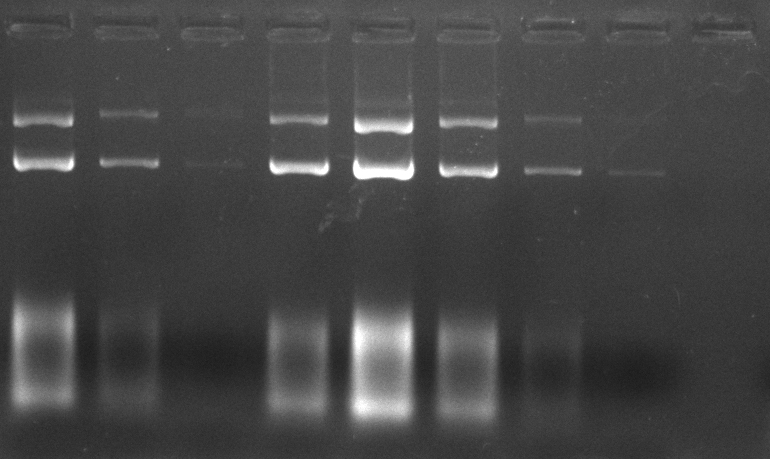
\includegraphics[width=7cm]{ima1}};
\begin{scope}[font=\scriptsize]
\node at (-3.15,2.3) {1};
\node at (-2.35,2.3) {2};
\node at (-1.55,2.3) {3};
\node at (-0.8,2.3) {4};
\node at (0,2.3) {5};
\node at (0.75,2.3) {6};
\node at (1.55,2.3) {7};
\node at (2.3,2.3) {8};
\node at (3.1,2.3) {9};
\draw (3.6,1.15) -- (3.75,1.15) -- (3.85,1.45) -- (4,1.45)  node[right] {gDNA};
\draw (3.6,1) -- (4,1) node[right] {pDNA (oc)};
\draw (3.6,0.55) -- (4,0.55) node[right] {pDNA (sc)};
\draw (3.6,-1) -- (4,-1) node[right] {RNA HMw};
\draw (3.6,-1.6) -- (4,-1.6) node[right] {RNA LMw};
\end{scope}
\end{tikzpicture}
\caption[Eletroforese em gel de agarose ao longo do processo de diafiltração]{Eletroforese em gel de agarose das amostras ao longo do processo de diafiltração: (1) Solução inicial (lisado); (2) permeado total recolhido; (3) concentrado após diafiltração; (4--8) amostras de permeado para VDF de 0.04, 0.15, 0.5, 1.5 e 2.5 respetivamente. (oc) indica a isoforma circular-aberta; (sc) indica a isoforma super-enrolada.}
\label{fig:2bart3}
\end{figure}
A técnica analítica de HIC utilizada para quantificar o DNA plasmídico (secção~\ref{subsubsec:2p3p1art3}) foi igualmente usada para obter informação sobre o conteúdo de contaminantes e consequentemente a sua remoção (ver capítulo~\ref{cha:pra}). De particular importância é a possibilidade de relacionar a permeação do RNA com a remoção dos contaminantes hidrofóbicos (ver apêndice~\ref{app:2}).
\index{contaminantes!hidrofóbicos}%
\index{contaminantes!RNA|see{RNA}}%
\index{contaminantes!DNA genómico|see{DNA genómico}}%
\index{contaminantes!proteínas|see{proteínas}}%
Como é possível ver na figura~\ref{fig:2aart3}, o rendimento de permeação dos contaminantes hidrofóbicos é por regra elevado na primeira operação de membranas, o que indica uma reduzida remoção do RNA presente. A análise por eletroforese, mostrada na figura~\ref{fig:2bart3}, confirma a ideia que o RNA permeia através da membrana juntamente com o pDNA. 

Proteínas e gDNA foram quantificados com os métodos descritos na secção~\ref{subsec:2p3art3}. Os dados para a remoção de gDNA e de proteína total, obtidos respetivamente por PCR em tempo real e pelo método do BCA, são indicados na tabela~\ref{tab:2art3}.
\index{PCR}%
\index{BCA}%
Observou-se baixa remoção de proteínas durante a diafiltração dos lisados (ver testes MF-A), em concordância com o baixo rendimento de contaminantes hidrofílicos verificado na análise de HIC. Os resultados mostram que existe uma tendência para o gDNA se re-dissolver, a partir do conteúdo sólido suspenso, tal como os valores negativos de remoção indicam.
\index{DNA genómico!redissolução}%
\index{tampão!diafiltração}%
Uma vez que é necessário que os sólidos suspensos contactem com o tampão de diafiltração durante o processo de filtração (para obter rendimentos de recuperação elevados de pDNA), durante a otimização de um sistema de filtração para aplicações em larga escala este resultado mostra que é necessário controlar as tensões de corte que atuam no material sólido para minimizar a degradação mecânica do gDNA precipitado e para evitar assim a sua re-solubilização.
\index{DNA genómico}%
\index{tensão de corte}%
É importante realçar que este aspeto não deve ser visto como uma desvantagem inerente aos processos de membranas quando comparados com a centrifugação. Na realidade são esperadas tensões de corte superiores, neste último processo, em centrífugas industriais \cite{prather,theo,chamsart,levy00}.
\index{centrifugação}%  
\begin{table}%
\centering
\caption[Proteína total e DNA genómico (gDNA) nos permeados após diafiltração]{Proteína total e DNA genómico (gDNA) nos permeados após diafiltração (microfiltração) com diferentes tampões e as suas remoções (\remocaoum) na operação de difiltração (testes MF-A, MF-B e MF-C). Valores iniciais medidos nos lisados: 200\,\micro g/mL de proteína total e 13.4\,\micro g de gDNA.}
\label{tab:2art3}
\begin{threeparttable}
\begin{tabular*}{14cm}{l @{\extracolsep{\fill}} llll}
\toprule
Ensaio & Proteína [\micro g/mL] &  \remocaoum\ (\porcento) & gDNA [\micro g/mL] & \remocaoum (\porcento) \\
\midrule
MF-A & 61 & 7.7 & 43.0 & -865 \\
MF-B & 71 & -6.3 & 18.1 & -306 \\
MF-C & 172\tnote{a}/45 & 14\tnote{a}/33 & 2.4\tnote{a}/5.5 &71\tnote{a}/-44 \\
\bottomrule
\end{tabular*}
\begin{tablenotes}
\item[a]Imediatamente após precipitação com CaCl$_2$.
\end{tablenotes} 
\end{threeparttable}
\end{table}

\subsubsection{Ensaios MF-B}
\label{subsubsec:3p1p3art3}
\index{microfiltração!MF-B}%
Para tentar evitar a excessiva re-solubilização do gDNA investigou-se a possibilidade de manter a força iónica aproximadamente constante durante o processo de diafiltração, usando \tce{CH3COOK} 1\,M em Tris/HCl 10\,mM a pH 8.00 (tampão ``B'', secção~\ref{subsec:2p2art3}).
\index{tampão!MF-B}%
Estes ensaios foram denominados ensaios MF-B. Teoricamente, não é previsível que as permeações de pDNA e RNA, ou mesmo as suas polarizações de concentração se alterem, tal como indicado na figura~\ref{fig:3acart3}.
\begin{figure}
	\centering
	%!TEX root=testfigum.tex
\begin{tikzpicture}

%\draw[help lines] (0cm,0cm) grid (14cm,7cm);
\node[right,font=\scriptsize] at (0cm,4.75cm) {MF-B};
\node[right,font=\scriptsize] at (7cm,4.75cm) {MF-B};
\node[right,font=\large] at (0cm,5.5cm) {a)};
\node[right,font=\large] at (7cm,5.5cm) {b)};

\begin{axis}[%
%width=\figurewidth,
%height=\figureheight,
width=5cm,
height=5cm,
scale only axis,
xmin=0,
xmax=3,
xlabel={VDF},
ymin=0,
ymax=1.1,
ylabel={\permobs},
at={(0cm,0cm)},
anchor=south west,
name=plot1,
legend style={at={(6cm,-1.5cm)},legend columns=2,anchor=center,font=\scriptsize,draw=black,fill=white,legend cell align=left}
]
\addplot [
color=black,
solid,
%forget plot
]
table[row sep=crcr]{
0 0.9864253394\\
0.6558345643 0.9841628959\\
1.369276219 0.9864253394\\
1.861152142 0.9864253394\\
2.144756278 0.9864253394\\
2.614475628 0.9864253394\\
3 0.9864253394\\
};
\addlegendentry{\pVAX};

\addplot [
color=black,
dashed,
%forget plot
]
table[row sep=crcr]{
0 0.9954751131\\
0.2304283604 0.9954751131\\
0.5228951256 0.9977375566\\
0.8153618907 1\\
1.183161004 1\\
1.568685377 1\\
1.905465288 1\\
2.353028065 1\\
2.694239291 1\\
3 1\\
};
\addlegendentry{RNA 23\,S};

\addplot [
color=black,
dash pattern=on 1pt off 3pt on 3pt off 3pt,
%forget plot
]
table[row sep=crcr]{
0 0.9954751131\\
0.1949778434 0.9977375566\\
0.4342688331 0.9977375566\\
0.7355982275 1\\
1.107828656 1\\
1.435745938 1\\
1.772525849 1\\
2.104874446 1\\
2.627769572 0.9977375566\\
2.871491876 1\\
3 0.9977375566\\
};
\addlegendentry{RNA 16\,S};

\addplot [
color=black,
dotted,
%forget plot
]
table[row sep=crcr]{
0 0.9932126697\\
0.2481536189 0.9954751131\\
0.4963072378 0.9977375566\\
0.8242245199 0.9954751131\\
1.307237814 0.9977375566\\
1.688330871 0.9977375566\\
2.082717873 0.9977375566\\
2.742983752 0.9954751131\\
3 0.9977375566\\
};
\addlegendentry{RNA 5\,S};
\end{axis}

\begin{axis}[%
%width=\figurewidth,
%height=\figureheight,
width=5cm,
height=5cm,
scale only axis,
xmin=0,
xmax=3,
xlabel={VDF},
ymin=0,
ymax=2,
ylabel={\concm/\concb},
at={(7cm,0cm)},
anchor=south west,
%legend style={at={(0.97,0.03)},anchor=south east,font=\scriptsize,draw=black,fill=white,legend cell align=left}
]
\addplot [
color=black,
solid
]
table[row sep=crcr]{
0 1.679671458\\
0.5672082718 1.675564682\\
1.564254062 1.679671458\\
1.989660266 1.679671458\\
2.570162482 1.679671458\\
3 1.679671458\\
};
%\addlegendentry{\pVAX};

\addplot [
color=black,
dashed
]
table[row sep=crcr]{
0 1.162217659\\
0.3545051699 1.170431211\\
0.8197932053 1.170431211\\
1.280649926 1.170431211\\
1.732644018 1.174537988\\
2.184638109 1.170431211\\
2.649926145 1.170431211\\
3 1.170431211\\
};
%\addlegendentry{RNA 23\,S};

\addplot [
color=black,
dash pattern=on 1pt off 3pt on 3pt off 3pt
]
table[row sep=crcr]{
0 1.133470226\\
0.2880354505 1.133470226\\
0.9704579025 1.133470226\\
1.550960118 1.133470226\\
2.016248154 1.133470226\\
2.592319055 1.133470226\\
3 1.137577002\\
};
%\addlegendentry{RNA 16\,S};

\addplot [
color=black,
dotted
]
table[row sep=crcr]{
0 1.075975359\\
0.4165435746 1.075975359\\
0.8995568685 1.075975359\\
1.382570162 1.071868583\\
1.856720827 1.075975359\\
2.251107829 1.075975359\\
2.579025111 1.075975359\\
3 1.075975359\\
};
%\addlegendentry{RNA 5\,S};

\end{axis}
\end{tikzpicture}%
	\caption[Previsão das permeações e da polarização de concentração (MF-B)]{Permeações observadas (a) e polarização de concentração (b), para as várias espécies, em função do fator de diluição volumétrico (VDF) para os ensaios MF-B.}
	\label{fig:3acart3}
\end{figure}

Os resultados experimentais, apresentados na figura~\ref{fig:3eart3}, confirmam que a permeação de pDNA e dos contaminantes permanece elevada, com um ligeiro aumento no rendimento de recuperação do DNA plasmídico, que se observou ser (92.4$\pm$0.4)\porcento\ nestas condições. A retenção do pDNA foi de (4.4$\pm$0.1)\porcento, sugerindo assim um decréscimo na adsorção, o que conduz a uma melhor aproximação entre os resultados experimentais e as previsões teóricas. Como é possível verificar na tabela~\ref{tab:2art3}, a remoção de proteínas permaneceu baixa, mas observou-se uma variação significativa no conteúdo de gDNA nos permeados, obtendo-se uma redução de cerca de 60\%.
\index{DNA genómico!rendimento de remoção (MF)}%
\index{proteínas!rendimento de remoção (MF)}%
Este resultado sugere que a re-dissolução de gDNA pode de facto ser reduzida aumentando a força iónica do tampão de diafiltração. É possível que este aumento da força iónica possa ter dado origem a menores valores de re-dissolução de outros contaminantes, o que pode ter conduzido a uma menor adsorção do plasmídeo na membrana. 
\begin{figure}
	\centering
	\setlength\figureheight{6cm} 
	\setlength\figurewidth{6cm}
	% This file was created by matlab2tikz v0.3.3.
% Copyright (c) 2008--2013, Nico Schlömer <nico.schloemer@gmail.com>
% All rights reserved.
% 
% The latest updates can be retrieved from
%   http://www.mathworks.com/matlabcentral/fileexchange/22022-matlab2tikz
% where you can also make suggestions and rate matlab2tikz.
% 
% 
% 
\begin{tikzpicture}
%\draw[help lines] (-2,-2) grid (10,10);
\node[right,font=\scriptsize] at (0,5.75) {MF-B}; 
\begin{axis}[%
width=\figurewidth,
height=\figureheight,
scale only axis,
xmin=0,
xmax=3.2,
xlabel={VDF},
ymin=0,
ymax=1.05,
ylabel={Rendimento de permeação},
legend style={at={(1.03,0.5)},anchor=west,font=\scriptsize,draw=black,fill=white,legend cell align=left}
]
\addplot [
color=black,
solid
]
table[row sep=crcr]{
0 -0.002155172414\\
0.08035714286 0.05603448276\\
0.2142857143 0.1530172414\\
0.375 0.2693965517\\
0.5669642857 0.3943965517\\
0.7544642857 0.5\\
0.9508928571 0.5862068966\\
1.174107143 0.6745689655\\
1.441964286 0.7521551724\\
1.866071429 0.8405172414\\
2.174107143 0.8857758621\\
2.549107143 0.9288793103\\
2.852678571 0.9504310345\\
3 0.9590517241\\
};
\addlegendentry{Permeação total};

\addplot [
color=black,
only marks,
mark=*,
mark options={solid,fill=white,draw=black}
]
table[row sep=crcr]{
0.04464 0.004310344828\\
0.04464 0.008620689655\\
0.1517857143 0.07327586207\\
0.1517857143 0.08836206897\\
0.5 0.3534482759\\
0.5 0.3642241379\\
1.5 0.7564655172\\
1.5 0.7737068966\\
2.5 0.8706896552\\
2.5 0.8836206897\\
3 0.9181034483\\
3 0.9245689655\\
};
\addlegendentry{\pVAX};

\addplot [
color=black,
only marks,
mark=triangle*,
mark options={solid,,rotate=180,fill=black,draw=black}
]
table[row sep=crcr]{
0.04464 0.002155172414\\
0.04464 0.01293103448\\
0.1517857143 0.09482758621\\
0.1517857143 0.07974137931\\
0.5 0.3534482759\\
0.5 0.3728448276\\
1.5 0.7543103448\\
1.5 0.7931034483\\
2.5 0.9288793103\\
2.5 0.8771551724\\
3 0.9418103448\\
3 0.9892241379\\
};
\addlegendentry{C. hidrofílicos};

\addplot [
color=black,
only marks,
mark=triangle*,
mark options={solid,fill=white,draw=black}
]
table[row sep=crcr]{
0.04464 0.002155172414\\
0.1517857143 0.06896551724\\
0.5 0.3362068966\\
0.5 0.3836206897\\
1.5 0.7392241379\\
1.5 0.8168103448\\
2.5 0.8577586207\\
2.5 0.974137931\\
3 0.9181034483\\
3 0.9181034483\\
};
\addlegendentry{C. hidrofóbicos};

\end{axis}
\end{tikzpicture}%
	\caption[Rendimentos de permeação de pDNA e contaminantes (MF-B)]{Rendimentos de permeação do pDNA, contaminantes hidrofílicos e contaminantes hidrofóbicos em função do fator de diluição volumétrico, para os ensaios MF-B.}
	\label{fig:3eart3}
\end{figure}

\subsubsection{Ensaios MF-C}
\label{subsubsec:3p1p4art3}
\index{microfiltração!MF-C}%
Estudou-se um novo aumento da força iónica da solução pela adição de 1\,M de \cacldois\ aos lisados, antes da diafiltração, e pelo uso do tampão ``C'' (ver secção~\ref{subsec:2p2art3}).
\index{tampão!MF-C}%
\index{cloreto de cálcio!microfiltração}%
A utilização do \cacldois\ teve também como finalidade precipitar o RNA presente. Estes ensaios são denominados ensaios MF-C. A adição de \cacldois\ aos lisados foi estudada previamente por Eon-Duval \et\ \cite{duvaltff,duval2} onde se demonstrou a eficácia deste sal na remoção de RNA por precipitação.
\index{cloreto de cálcio!precipitação de RNA}%
Pela aplicação do modelo, é esperado que a adição de 1\,M de \cacldois\ aos lisados não afete as permeações e polarização de concentração do plasmídeo e das várias espécies de RNA, tal como se pode verificar na figura~\ref{fig:3bdart3}. Só é esperado uma alteração para um poro com um raio inferior a 10\,nm, tal como se pode ver comparando a figura~\ref{fig:1art3}~(a) com a figura~\ref{fig:4abart3}~(a), e a figura~\ref{fig:1art3}~(b) com a figura~\ref{fig:4abart3}~(b), respetivamente. Os cromatogramas de HIC dos lisados, antes e depois da adição de \cacldois, mostrados na figura~\ref{fig:4cart3}, indicam que a concentração de pDNA não é afetada pela adição de \cacldois, ao mesmo tempo que mostram a elevada remoção dos contaminantes hidrofóbicos, tal como esperado.
\index{lisado!HIC}%
Durante o processo de diafiltração, a concentração destes compostos manteve-se muito reduzida, tal como se pode verificar a partir dos valores de remoção mostrados na figura~\ref{fig:3fart3}. Obteve-se um rendimento de remoção destes contaminantes de 91\% no final da diafiltração.
\index{contaminantes!rendimento de remoção}%
A análise por eletroforese, mostrada na figura~\ref{fig:4dart3}, confirma a elevada remoção do RNA conseguida com a adição de \cacldois, onde se pode constatar que praticamente todo o RNA de alto peso molecular (HMw\,RNA) e a maior parte do RNA de baixo peso molecular (LMw\,RNA), presente inicialmente nos lisados, é removido antes da diafiltração.
\index{AGE}%
Os contaminantes que não precipitam com a adição de \cacldois\ permeiam livremente pela membrana, tal como se pode verificar pelos valores de remoção obtidos exclusivamente para o passo de filtração, estando estes valores indicados na figura~\ref{fig:3fart3}, onde são denominados por ``apenas filtração''. Para além da elevada remoção de RNA obtida com a adição de \cacldois\ aos lisados, verificou-se também alguma precipitação de proteínas e especialmente gDNA (ver tabela~\ref{tab:2art3}). No entanto observou-se também uma maior adsorção de pDNA em comparação com os ensaios anteriores, cerca de 15\%, como indicam os valores de rendimento de permeação, (84$\pm$1)\%, e de retenção, (0.3$\pm$0.1)\%.\index{DNA plasmídico!adsorção}
\begin{figure}[!t]
	\centering
	%!TEX root=testfigum.tex
\begin{tikzpicture}

%\draw[help lines] (0cm,0cm) grid (14cm,7cm);
\node[right,font=\scriptsize] at (0cm,4.75cm) {MF-C};
\node[right,font=\scriptsize] at (7cm,4.75cm) {MF-C};
\node[right,font=\large] at (0,5.5) {a)};
\node[right,font=\large] at (7,5.5) {b)};

\begin{axis}[%
%width=\figurewidth,
%height=\figureheight,
width=5cm,
height=5cm,
scale only axis,
xmin=0,
xmax=3,
xlabel={VDF},
ymin=0,
ymax=1.1,
ylabel={\permobs},
at={(0cm,0cm)},
anchor=south west,
name=plot1,
legend style={at={(6cm,-1.5cm)},legend columns=2,anchor=center,font=\scriptsize,draw=black,fill=white,legend cell align=left}
]
\addplot [
color=black,
solid,
%forget plot
]
table[row sep=crcr]{
0 0.993227991 \\
1.544247788 0.993227991\\
2.654867257 0.993227991\\
3 0.993227991\\
};
\addlegendentry{\pVAX};

\addplot [
color=black,
dashed,
%forget plot
]
table[row sep=crcr]{
0.004424779 0.993227991\\
0.530973451 0.997742664\\
1.911504425 0.997742664\\
2.694690265 0.997742664\\
3 0.997742664\\
};
\addlegendentry{RNA 23\,S};

\addplot [
color=black,
dash pattern=on 1pt off 3pt on 3pt off 3pt,
%forget plot
]
table[row sep=crcr]{
0 0.995485327\\
0.654867257 0.995485327\\
1.628318584 0.993227991\\
2.305309735 0.995485327\\
2.787610619 0.995485327\\
3 0.995485327\\
};
\addlegendentry{RNA 16\,S};

\addplot [
color=black,
dotted,
%forget plot
]
table[row sep=crcr]{
0 0.995485327\\
0.867256637 0.995485327\\
2.110619469 0.997742664\\
2.738938053 0.995485327\\
2.995575221 0.995485327\\
};
\addlegendentry{RNA 5\,S};
\end{axis}

\begin{axis}[%
%width=\figurewidth,
%height=\figureheight,
width=5cm,
height=5cm,
scale only axis,
xmin=0,
xmax=3,
xlabel={VDF},
ymin=0,
ymax=2,
ylabel={\concm/\concb},
at={(7cm,0cm)},
anchor=south west,
%legend style={at={(0.97,0.03)},anchor=south east,font=\scriptsize,draw=black,fill=white,legend cell align=left}
]
\addplot [
color=black,
solid
]
table[row sep=crcr]{
0	1.503080082\\
1.728212703	1.503080082\\
3	1.503080082\\
};
%\addlegendentry{\pVAX};

\addplot [
color=black,
dashed
]
table[row sep=crcr]{
0	1.170431211
1.426883309	1.170431211\\
2.042836041	1.170431211\\
3	1.170431211\\
};
%\addlegendentry{RNA 23\,S};

\addplot [
color=black,
dash pattern=on 1pt off 3pt on 3pt off 3pt
]
table[row sep=crcr]{
0.00E+00	1.137577002\\
1.316100443	1.133470226\\
2.127031019	1.137577002\\
3	1.137577002\\
};
%\addlegendentry{RNA 16\,S};

\addplot [
color=black,
dotted
]
table[row sep=crcr]{
0.00E+00	1.071868583\\
0.740029542	1.071868583\\
1.612998523	1.071868583\\
2.246676514	1.071868583\\
3	1.075975359\\
};
%\addlegendentry{RNA 5\,S};

\end{axis}
\end{tikzpicture}%
	\caption[Previsão das permeações e da polarização de concentração (MF-C)]{Permeações observadas (a) e polarização de concentração (b), para as várias espécies, em função do fator de diluição volumétrico (VDF) para os ensaios MF-C.}
	\label{fig:3bdart3}
\end{figure}
\begin{figure}[!t]
	\centering
	%!TEX root=testfigum.tex
\begin{tikzpicture}

%\draw[help lines] (0cm,0cm) grid (14cm,7cm);
\node[right,font=\scriptsize] at (0cm,4.75cm) {CaCl$_2$\ 1\,M};
\node[left,font=\scriptsize] at (12cm,4.75cm) {CaCl$_2$\ 1\,M};
\node[right,font=\large] at (0,5.5) {a)};
\node[right,font=\large] at (7,5.5) {b)};

\begin{axis}[%
%width=\figurewidth,
%height=\figureheight,
width=5cm,
height=5cm,
scale only axis,
xmode=log,
xmin=1,
xmax=100,
xminorticks=true,
xlabel={\raioporo\,[nm]},
ymin=0,
ymax=1.1,
ylabel={\permobs},
at={(0cm,5cm)},
anchor=north west,
name=plot1,
legend style={at={(6cm,-1.5cm)},legend columns=2,anchor=center,font=\scriptsize,draw=black,fill=white,legend cell align=left}
]
\addplot [
color=black,
solid,
%forget plot
]
table[row sep=crcr]{
1 0.018480493\\
1.4 0.039014374\\
1.89 0.063655031\\
2.23 0.084188912\\
2.73 0.12936345\\
3.35 0.193018481\\
3.97 0.275154004\\
4.58 0.369609856\\
5.21 0.464065708\\
6.01 0.59137577\\
6.98 0.751540041\\
7.94 0.90349076\\
8.85 0.975359343\\
9.87 0.995893224\\
13.85 1\\
100 1\\
};
\addlegendentry{\pVAX};

\addplot [
color=black,
dashed,
%forget plot
]
table[row sep=crcr]{
1 0.232032854\\
1.15 0.316221766\\
1.38 0.41889117\\
1.77 0.626283368\\
2.07 0.76386037\\
2.62 0.90349076\\
3.19 0.969199179\\
4.08 0.997946612\\
5.58 1\\
100 1\\
};
\addlegendentry{RNA 23\,S};

\addplot [
color=black,
dash pattern=on 1pt off 3pt on 3pt off 3pt,
%forget plot
]
table[row sep=crcr]{
1 0.400410678\\
1.15 0.509240246\\
1.35 0.62422998\\
1.58 0.737166324\\
1.91 0.850102669\\
2.62 0.944558522\\
3.84 0.981519507\\
5.65 0.993839836\\
8.38 0.997946612\\
22.14 0.997946612\\
100 1\\
};
\addlegendentry{RNA 16\,S};

\addplot [
color=black,
dotted,
%forget plot
]
table[row sep=crcr]{
1 0.515400411\\
1.26 0.609856263\\
1.77 0.751540041\\
2.47 0.856262834\\
3.61 0.917864476\\
5.17 0.952772074\\
8.32 0.979466119\\
13.67 0.991786448\\
19.72 0.995893224\\
39.17 1\\
100 1\\
};
\addlegendentry{RNA 5\,S};
\end{axis}

\begin{axis}[%
%width=\figurewidth,
%height=\figureheight,
width=5cm,
height=5cm,
scale only axis,
xmode=log,
xmin=1,
xmax=100,
xlabel={\raioporo\,[nm]},
ymin=-10,
ymax=120,
ylabel={\concm/\concb},
at={(7cm,0cm)},
anchor=south west,
%legend style={at={(0.97,0.97)},anchor=north east,font=\scriptsize,draw=black,fill=white,legend cell align=left}
]
\addplot [
color=black,
solid
]
table[row sep=crcr]{
1 56.18069815\\
1.50675119 55.68788501\\
2.498193723 55.44147844\\
3.764156364 55.44147844\\
4.781071325 53.71663244\\
6.156267855 51.00616016\\
7.505349485 47.06365503\\
8.42977579 41.88911704\\
9.598333721 33.75770021\\
11.62202751 24.64065708\\
13.88139889 17.49486653\\
17.75244435 10.59548255\\
26.74851665 5.420944559\\
42.56769351 2.95687885\\
69.14529137 1.971252567\\
100 1.478439425\\
};
%\addlegendentry{\pVAX};

\addplot [
color=black,
dashed
]
table[row sep=crcr]{
1.261508577 120\\
1.496491257 114.3326489\\
1.703938854 108.4188912\\
1.874981697 102.9979466\\
2.063193967 95.35934292\\
2.239486083 86.98151951\\
2.549929597 71.70431211\\
2.786787524 62.83367556\\
3.066527645 53.96303901\\
3.713068298 37.94661191\\
4.227783696 30.06160164\\
5.154258219 20.94455852\\
6.457865875 13.30595483\\
9.664139821 6.652977413\\
15.6980496 3.449691992\\
24.30841695 1.971252567\\
41.13801413 1.232032854\\
79.27017044 0.985626283\\
100 1.232032854\\
};
%\addlegendentry{RNA 23\,S};

\addplot [
color=black,
dash pattern=on 1pt off 3pt on 3pt off 3pt
]
table[row sep=crcr]{
1.085446215 120.2464066\\
1.252918577 109.650924\\
1.407239291 101.5195072\\
1.613299999 89.19917864\\
1.751150378 81.31416838\\
1.874981697 74.16837782\\
2.105921297 61.60164271\\
2.447507524 48.04928131\\
2.943355571 34.25051335\\
3.868450927 20.69815195\\
4.684067506 14.78439425\\
6.820683433 7.392197125\\
10 4.188911704\\
14.66128739 2.710472279\\
21.79108888 1.724845996\\
33.28550827 1.232032854\\
78.19429601 0.985626283\\
100 1.232032854\\
};
%\addlegendentry{RNA 16\,S};

\addplot [
color=black,
dotted
]
table[row sep=crcr]{
1.027707288 0.492813142\\
1.763156251 0.739219713\\
3.216758058 0.985626283\\
5.789102992 0.985626283\\
10.92888027 0.985626283\\
17.87415497 0.985626283\\
25.1532132 0.985626283\\
41.7040317 0.985626283\\
67.742393 0.985626283\\
100 0.985626283\\
};
%\addlegendentry{RNA 5\,S};

\end{axis}
\end{tikzpicture}%
	\caption[Permeação e da polarização de concentração em função de \raioporo\ (MF-C)]{Previsão das permeações observadas (a) e da polarização de concentração (b) para o plasmídeo (usando o modelo CSC) e para as várias espécies de RNA (usando o modelo FJC), para as condições experimentais dos ensaios MF-C.}
	\label{fig:4abart3}
\end{figure}
\begin{figure}[!t]
	\centering
	\setlength\figureheight{6cm} 
	\setlength\figurewidth{6cm}
	% This file was created by matlab2tikz v0.3.3.
% Copyright (c) 2008--2013, Nico Schlömer <nico.schloemer@gmail.com>
% All rights reserved.
% 
% The latest updates can be retrieved from
%   http://www.mathworks.com/matlabcentral/fileexchange/22022-matlab2tikz
% where you can also make suggestions and rate matlab2tikz.
% 
% 
% 
\begin{tikzpicture}

%\draw[help lines] (-2,-1) grid (12,10);
\node[right,font=\scriptsize] at (0,5.75) {HIC};

\begin{axis}[%
width=\figurewidth,
height=\figureheight,
scale only axis,
xmin=0,
xmax=8,
xlabel={\volretencao\,[mL]},
ymin=-100,
ymax=1400,
ylabel={Absorvância 260\,nm\,[mAU]},
legend style={at={(1.03,0.5)},anchor=west,font=\scriptsize,draw=black,fill=white,legend cell align=left}
]
\addplot [
color=black,
solid
]
table[row sep=crcr]{
0 -0.019\\
0.01 -0.027\\
0.02 -0.035\\
0.0299 -0.036\\
0.0399 -0.03\\
0.0499 -0.033\\
0.0599 -0.037\\
0.0699 -0.036\\
0.0799 -0.035\\
0.0898 -0.027\\
0.0998 -0.014\\
0.1098 -0.007\\
0.1198 0\\
0.1298 0.004\\
0.1398 0.003\\
0.1497 0.01\\
0.1597 -0.001\\
0.1697 -0.004\\
0.1797 -0.009\\
0.1897 -0.016\\
0.1997 -0.011\\
0.2096 -0.009\\
0.2196 -0.008\\
0.2296 -0.003\\
0.2396 -0.005\\
0.2496 -0.001\\
0.2596 -0.002\\
0.2695 -0.004\\
0.2795 0.003\\
0.2895 0.007\\
0.2995 0.014\\
0.3095 0.018\\
0.3195 0.012\\
0.3294 0.001\\
0.3394 -0.008\\
0.3494 -0.015\\
0.3594 -0.013\\
0.3694 -0.005\\
0.3794 -0.009\\
0.3893 -0.012\\
0.3993 -0.015\\
0.4093 -0.018\\
0.4193 -0.015\\
0.4293 -0.009\\
0.4393 -0.001\\
0.4492 0.002\\
0.4592 0.002\\
0.4692 -0.005\\
0.4792 -0.009\\
0.4892 -0.013\\
0.4992 -0.011\\
0.5091 -0.007\\
0.5191 -0.009\\
0.5291 -0.005\\
0.5391 -0.001\\
0.5491 -0.006\\
0.5591 -0.007\\
0.569 -0.01\\
0.579 -0.012\\
0.589 -0.002\\
0.599 0.002\\
0.609 0.01\\
0.619 0.021\\
0.6289 0.19\\
0.6389 1.395\\
0.6489 6.534\\
0.6589 20.878\\
0.6689 49.858\\
0.6788 93.094\\
0.6888 141.194\\
0.6988 182.108\\
0.7088 206.022\\
0.7188 209.901\\
0.7288 198.133\\
0.7387 178.908\\
0.7487 159.052\\
0.7587 141.27\\
0.7687 125.977\\
0.7787 112.866\\
0.7887 101.507\\
0.7986 91.696\\
0.8086 82.938\\
0.8186 74.954\\
0.8286 67.661\\
0.8386 61.03\\
0.8486 54.997\\
0.8585 49.571\\
0.8685 44.715\\
0.8785 40.339\\
0.8885 36.396\\
0.8985 32.872\\
0.9085 29.73\\
0.9184 26.929\\
0.9284 24.477\\
0.9384 22.286\\
0.9484 20.32\\
0.9584 18.569\\
0.9684 17.008\\
0.9783 15.614\\
0.9883 14.391\\
0.9983 13.292\\
1.0083 12.302\\
1.0183 11.392\\
1.0283 10.573\\
1.0382 9.826\\
1.0482 9.145\\
1.0582 8.556\\
1.0682 8.023\\
1.0782 7.543\\
1.0882 7.129\\
1.0981 6.805\\
1.1081 6.65\\
1.1181 6.831\\
1.1281 7.776\\
1.1381 10.318\\
1.1481 15.964\\
1.158 26.751\\
1.168 43.73\\
1.178 65.65\\
1.188 90.042\\
1.198 115.814\\
1.208 143.843\\
1.2179 176.43\\
1.2279 215.003\\
1.2379 257.983\\
1.2479 300.647\\
1.2579 337.134\\
1.2679 364.247\\
1.2778 381.575\\
1.2878 390.139\\
1.2978 391.8\\
1.3078 388.54\\
1.3178 381.851\\
1.3277 372.628\\
1.3377 361.564\\
1.3477 349.15\\
1.3577 335.722\\
1.3677 321.637\\
1.3777 307.336\\
1.3876 293\\
1.3976 278.823\\
1.4076 264.965\\
1.4176 251.523\\
1.4276 238.515\\
1.4376 225.967\\
1.4475 214.022\\
1.4575 202.547\\
1.4675 191.575\\
1.4775 181.196\\
1.4875 171.418\\
1.4975 162.227\\
1.5074 153.667\\
1.5174 145.72\\
1.5274 138.329\\
1.5374 131.535\\
1.5474 125.387\\
1.5574 119.91\\
1.5673 115.161\\
1.5773 111.266\\
1.5873 108.282\\
1.5973 106.281\\
1.6073 105.356\\
1.6173 105.601\\
1.6272 107.076\\
1.6372 109.758\\
1.6472 113.688\\
1.6572 118.754\\
1.6672 124.737\\
1.6772 131.422\\
1.6871 138.575\\
1.6971 145.945\\
1.7071 153.198\\
1.7171 160.127\\
1.7271 166.544\\
1.7371 172.221\\
1.747 177.006\\
1.757 180.904\\
1.767 183.675\\
1.777 185.395\\
1.787 186.136\\
1.797 185.971\\
1.8069 185.004\\
1.8169 183.284\\
1.8269 180.932\\
1.8369 178.072\\
1.8469 174.758\\
1.8569 171.015\\
1.8668 167.191\\
1.8768 163.239\\
1.8868 159.093\\
1.8968 155.139\\
1.9068 151.314\\
1.9168 147.53\\
1.9267 144.013\\
1.9367 140.911\\
1.9467 138.162\\
1.9567 135.824\\
1.9667 134.278\\
1.9766 133.964\\
1.9866 135.041\\
1.9966 137.163\\
2.0066 139.688\\
2.0166 142.054\\
2.0266 143.534\\
2.0365 144.044\\
2.0465 143.93\\
2.0565 143.427\\
2.0665 142.655\\
2.0765 141.606\\
2.0865 140.351\\
2.0964 138.954\\
2.1064 137.489\\
2.1164 135.923\\
2.1264 134.345\\
2.1364 132.716\\
2.1464 131.055\\
2.1563 129.395\\
2.1663 127.614\\
2.1763 125.381\\
2.1863 122.603\\
2.1963 119.269\\
2.2063 115.504\\
2.2162 111.339\\
2.2262 107.073\\
2.2362 102.903\\
2.2462 98.825\\
2.2562 94.88\\
2.2662 91.154\\
2.2761 87.489\\
2.2861 84.053\\
2.2961 80.802\\
2.3061 77.721\\
2.3161 74.893\\
2.3261 72.308\\
2.336 69.821\\
2.346 67.468\\
2.356 65.325\\
2.366 63.372\\
2.376 61.526\\
2.386 59.845\\
2.3959 58.307\\
2.4059 56.909\\
2.4159 55.681\\
2.4259 54.601\\
2.4359 53.581\\
2.4459 52.606\\
2.4558 51.684\\
2.4658 50.803\\
2.4758 49.953\\
2.4858 49.17\\
2.4958 48.465\\
2.5058 47.849\\
2.5157 47.3\\
2.5257 46.723\\
2.5357 45.997\\
2.5457 45.092\\
2.5557 43.969\\
2.5657 42.704\\
2.5756 41.45\\
2.5856 40.263\\
2.5956 38.516\\
2.6056 37.265\\
2.6156 37.044\\
2.6255 36.901\\
2.6355 36.632\\
2.6455 36.091\\
2.6555 35.367\\
2.6655 34.631\\
2.6755 34.027\\
2.6854 33.598\\
2.6954 33.238\\
2.7054 32.899\\
2.7154 32.589\\
2.7254 32.3\\
2.7354 32.028\\
2.7453 31.766\\
2.7553 31.511\\
2.7653 31.266\\
2.7753 31.028\\
2.7853 30.799\\
2.7953 30.589\\
2.8052 30.39\\
2.8152 30.193\\
2.8252 30.004\\
2.8352 29.816\\
2.8452 29.626\\
2.8552 29.452\\
2.8651 29.293\\
2.8751 29.143\\
2.8851 28.994\\
2.8951 28.84\\
2.9051 28.687\\
2.9151 28.53\\
2.925 28.383\\
2.935 28.251\\
2.945 28.132\\
2.955 28.017\\
2.965 27.899\\
2.975 27.779\\
2.9849 27.655\\
2.9949 27.537\\
3.0049 27.43\\
3.0149 27.335\\
3.0249 27.237\\
3.0349 27.127\\
3.0448 27.017\\
3.0548 26.917\\
3.0648 26.839\\
3.0748 26.768\\
3.0848 26.694\\
3.0948 26.617\\
3.1047 26.522\\
3.1147 26.426\\
3.1247 26.347\\
3.1347 26.275\\
3.1447 26.206\\
3.1547 26.135\\
3.1646 26.055\\
3.1746 25.973\\
3.1846 25.895\\
3.1946 25.836\\
3.2046 25.796\\
3.2146 25.755\\
3.2245 25.71\\
3.2345 25.654\\
3.2445 25.576\\
3.2545 25.482\\
3.2645 25.383\\
3.2745 25.295\\
3.2844 25.216\\
3.2944 25.139\\
3.3044 25.071\\
3.3144 24.988\\
3.3244 24.9\\
3.3343 24.828\\
3.3443 24.76\\
3.3543 24.709\\
3.3643 24.656\\
3.3743 24.592\\
3.3843 24.524\\
3.3942 24.448\\
3.4042 24.383\\
3.4142 24.332\\
3.4242 24.283\\
3.4342 24.225\\
3.4442 24.163\\
3.4541 24.101\\
3.4641 24.028\\
3.4741 23.958\\
3.4841 23.9\\
3.4941 23.838\\
3.5041 23.777\\
3.514 23.709\\
3.524 23.632\\
3.534 23.554\\
3.544 23.479\\
3.554 23.425\\
3.564 23.386\\
3.5739 23.34\\
3.5839 23.284\\
3.5939 23.214\\
3.6039 23.129\\
3.6139 23.05\\
3.6239 22.98\\
3.6338 22.924\\
3.6438 22.87\\
3.6538 22.816\\
3.6638 22.758\\
3.6738 22.69\\
3.6838 22.622\\
3.6937 22.563\\
3.7037 22.508\\
3.7137 22.452\\
3.7237 22.395\\
3.7337 22.33\\
3.7437 22.259\\
3.7536 22.194\\
3.7636 22.132\\
3.7736 22.076\\
3.7836 22.027\\
3.7936 21.974\\
3.8036 21.911\\
3.8135 21.846\\
3.8235 21.778\\
3.8335 21.718\\
3.8435 21.672\\
3.8535 21.632\\
3.8635 21.592\\
3.8734 21.549\\
3.8834 21.497\\
3.8934 21.447\\
3.9034 21.411\\
3.9134 21.386\\
3.9234 21.36\\
3.9333 21.328\\
3.9433 21.282\\
3.9533 21.215\\
3.9633 21.149\\
3.9733 21.087\\
3.9832 21.046\\
3.9932 21.031\\
4.0032 21.034\\
4.0132 21.059\\
4.0232 21.104\\
4.0332 21.184\\
4.0431 21.319\\
4.0531 21.522\\
4.0631 21.791\\
4.0731 22.114\\
4.0831 22.478\\
4.0931 22.874\\
4.103 23.313\\
4.113 23.811\\
4.123 24.38\\
4.133 25.022\\
4.143 25.708\\
4.153 26.441\\
4.1629 27.195\\
4.1729 27.981\\
4.1829 28.819\\
4.1929 29.714\\
4.2029 30.673\\
4.2129 31.683\\
4.2228 32.725\\
4.2328 33.784\\
4.2428 34.869\\
4.2528 36.015\\
4.2628 37.226\\
4.2728 38.502\\
4.2827 39.833\\
4.2927 41.197\\
4.3027 42.583\\
4.3127 43.995\\
4.3227 45.48\\
4.3327 47.062\\
4.3426 48.726\\
4.3526 50.467\\
4.3626 52.277\\
4.3726 54.137\\
4.3826 56.057\\
4.3926 58.097\\
4.4025 60.273\\
4.4125 62.566\\
4.4225 64.981\\
4.4325 67.499\\
4.4425 70.082\\
4.4525 72.779\\
4.4624 75.607\\
4.4724 78.6\\
4.4824 81.758\\
4.4924 85.067\\
4.5024 88.524\\
4.5124 92.168\\
4.5223 96.001\\
4.5323 99.838\\
4.5423 104.002\\
4.5523 108.416\\
4.5623 113.111\\
4.5723 117.794\\
4.5822 122.81\\
4.5922 128.01\\
4.6022 133.431\\
4.6122 139.181\\
4.6222 145.331\\
4.6321 151.463\\
4.6421 158.168\\
4.6521 165.342\\
4.6621 172.564\\
4.6721 180.001\\
4.6821 188.174\\
4.692 196.972\\
4.702 205.881\\
4.712 215.77\\
4.722 226.435\\
4.732 237.199\\
4.742 249.224\\
4.7519 261.725\\
4.7619 274.933\\
4.7719 289.045\\
4.7819 304.941\\
4.7919 321.354\\
4.8019 338.586\\
4.8118 356.464\\
4.8218 376.298\\
4.8318 396.392\\
4.8418 419.052\\
4.8518 442.328\\
4.8618 466.51\\
4.8717 491.102\\
4.8817 517.812\\
4.8917 544.121\\
4.9017 573.124\\
4.9117 602.431\\
4.9217 632.372\\
4.9316 662.205\\
4.9416 693.922\\
4.9516 724.759\\
4.9616 755.598\\
4.9716 786.274\\
4.9816 818.718\\
4.9915 849.367\\
5.0015 881.212\\
5.0115 911.081\\
5.0215 939.511\\
5.0315 966.774\\
5.0415 994.583\\
5.0514 1020.398\\
5.0614 1044.703\\
5.0714 1066.612\\
5.0814 1087.571\\
5.0914 1105.213\\
5.1014 1122.165\\
5.1113 1136.911\\
5.1213 1149.573\\
5.1313 1159.813\\
5.1413 1168.177\\
5.1513 1173.283\\
5.1613 1176.21\\
5.1712 1177.179\\
5.1812 1176.304\\
5.1912 1173.521\\
5.2012 1168.471\\
5.2112 1161.162\\
5.2212 1151.598\\
5.2311 1140.219\\
5.2411 1127.596\\
5.2511 1113.821\\
5.2611 1098.699\\
5.2711 1082.26\\
5.281 1064.521\\
5.291 1045.222\\
5.301 1025.101\\
5.311 1004.692\\
5.321 983.791\\
5.331 962.31\\
5.3409 940.38\\
5.3509 917.796\\
5.3609 894.563\\
5.3709 871.307\\
5.3809 848.353\\
5.3909 825.488\\
5.4008 802.664\\
5.4108 780.055\\
5.4208 756.957\\
5.4308 733.805\\
5.4408 711.081\\
5.4508 688.889\\
5.4607 667.142\\
5.4707 645.836\\
5.4807 624.886\\
5.4907 603.815\\
5.5007 582.913\\
5.5107 562.613\\
5.5206 542.964\\
5.5306 523.813\\
5.5406 505.411\\
5.5506 487.065\\
5.5606 468.759\\
5.5706 450.788\\
5.5805 433.381\\
5.5905 416.573\\
5.6005 400.371\\
5.6105 384.796\\
5.6205 369.309\\
5.6305 353.947\\
5.6404 338.91\\
5.6504 324.382\\
5.6604 310.446\\
5.6704 297.185\\
5.6804 284.282\\
5.6904 271.606\\
5.7003 259.143\\
5.7103 247.032\\
5.7203 235.355\\
5.7303 224.232\\
5.7403 213.695\\
5.7503 203.486\\
5.7602 193.528\\
5.7702 183.824\\
5.7802 174.412\\
5.7902 165.429\\
5.8002 157.029\\
5.8102 148.999\\
5.8201 141.333\\
5.8301 133.898\\
5.8401 126.664\\
5.8501 119.698\\
5.8601 113.077\\
5.8701 106.939\\
5.88 101.12\\
5.89 95.41\\
5.9 90.277\\
5.91 85.153\\
5.92 80.064\\
5.9299 75.595\\
5.9399 71.275\\
5.9499 67.086\\
5.9599 63.377\\
5.9699 59.731\\
5.9799 56.107\\
5.9898 52.783\\
5.9998 49.76\\
6.0098 46.878\\
6.0198 44.096\\
6.0298 41.642\\
6.0398 39.256\\
6.0497 36.895\\
6.0597 34.813\\
6.0697 32.787\\
6.0797 30.854\\
6.0897 29.181\\
6.0997 27.523\\
6.1096 26.005\\
6.1196 24.561\\
6.1296 23.171\\
6.1396 21.87\\
6.1496 20.675\\
6.1596 19.579\\
6.1695 18.561\\
6.1795 17.604\\
6.1895 16.71\\
6.1995 15.852\\
6.2095 15.044\\
6.2195 14.299\\
6.2294 13.615\\
6.2394 12.978\\
6.2494 12.377\\
6.2594 11.803\\
6.2694 11.238\\
6.2794 10.708\\
6.2893 10.24\\
6.2993 9.818\\
6.3093 9.432\\
6.3193 9.072\\
6.3293 8.696\\
6.3393 8.31\\
6.3492 7.945\\
6.3592 7.616\\
6.3692 7.32\\
6.3792 7.066\\
6.3892 6.817\\
6.3992 6.556\\
6.4091 6.291\\
6.4191 6.041\\
6.4291 5.807\\
6.4391 5.592\\
6.4491 5.406\\
6.4591 5.231\\
6.469 5.056\\
6.479 4.883\\
6.489 4.709\\
6.499 4.539\\
6.509 4.386\\
6.519 4.253\\
6.5289 4.13\\
6.5389 3.998\\
6.5489 3.857\\
6.5589 3.712\\
6.5689 3.587\\
6.5788 3.462\\
6.5888 3.374\\
6.5988 3.28\\
6.6088 3.177\\
6.6188 3.074\\
6.6288 2.951\\
6.6387 2.845\\
6.6487 2.758\\
6.6587 2.68\\
6.6687 2.613\\
6.6787 2.537\\
6.6887 2.447\\
6.6986 2.346\\
6.7086 2.249\\
6.7186 2.177\\
6.7286 2.106\\
6.7386 2.034\\
6.7486 1.966\\
6.7585 1.875\\
6.7685 1.779\\
6.7785 1.695\\
6.7885 1.623\\
6.7985 1.554\\
6.8085 1.496\\
6.8184 1.442\\
6.8284 1.378\\
6.8384 1.3\\
6.8484 1.239\\
6.8584 1.187\\
6.8684 1.137\\
6.8783 1.085\\
6.8883 1.03\\
6.8983 0.95\\
6.9083 0.873\\
6.9183 0.806\\
6.9283 0.751\\
6.9382 0.705\\
6.9482 0.661\\
6.9582 0.604\\
6.9682 0.545\\
6.9782 0.491\\
6.9882 0.447\\
6.9981 0.418\\
7.0081 0.386\\
7.0181 0.348\\
7.0281 0.291\\
7.0381 0.232\\
7.0481 0.178\\
7.058 0.128\\
7.068 0.085\\
7.078 0.05\\
7.088 0.006\\
7.098 -0.036\\
7.108 -0.076\\
7.1179 -0.127\\
7.1279 -0.168\\
7.1379 -0.205\\
7.1479 -0.24\\
7.1579 -0.273\\
7.1679 -0.31\\
7.1778 -0.344\\
7.1878 -0.392\\
7.1978 -0.442\\
7.2078 -0.487\\
7.2178 -0.54\\
7.2277 -0.576\\
7.2377 -0.606\\
7.2477 -0.644\\
7.2577 -0.691\\
7.2677 -0.741\\
7.2777 -0.787\\
7.2876 -0.832\\
7.2976 -0.872\\
7.3076 -0.908\\
7.3176 -0.953\\
7.3276 -1.001\\
7.3376 -1.048\\
7.3475 -1.092\\
7.3575 -1.125\\
7.3675 -1.16\\
7.3775 -1.198\\
7.3875 -1.239\\
7.3975 -1.289\\
7.4074 -1.336\\
7.4174 -1.372\\
7.4274 -1.413\\
7.4374 -1.44\\
7.4474 -1.463\\
7.4574 -1.495\\
7.4673 -1.53\\
7.4773 -1.565\\
7.4873 -1.593\\
7.4973 -1.63\\
7.5073 -1.66\\
7.5173 -1.689\\
7.5272 -1.72\\
7.5372 -1.753\\
7.5472 -1.78\\
7.5572 -1.808\\
7.5672 -1.842\\
7.5772 -1.868\\
7.5871 -1.893\\
7.5971 -1.917\\
7.6071 -1.946\\
7.6171 -1.974\\
7.6271 -2.002\\
7.6371 -2.027\\
7.647 -2.046\\
7.657 -2.063\\
7.667 -2.084\\
7.677 -2.113\\
7.687 -2.157\\
7.697 -2.194\\
7.7069 -2.226\\
7.7169 -2.252\\
7.7269 -2.269\\
7.7369 -2.297\\
7.7469 -2.331\\
7.7569 -2.361\\
7.7668 -2.392\\
7.7768 -2.421\\
7.7868 -2.45\\
7.7968 -2.479\\
7.8068 -2.507\\
7.8168 -2.546\\
7.8267 -2.587\\
7.8367 -2.628\\
7.8467 -2.666\\
7.8567 -2.693\\
7.8667 -2.714\\
7.8766 -2.736\\
7.8866 -2.769\\
7.8966 -2.808\\
7.9066 -2.835\\
7.9166 -2.855\\
7.9266 -2.867\\
7.9365 -2.884\\
7.9465 -2.924\\
7.9565 -2.974\\
7.9665 -3.022\\
7.9765 -3.058\\
7.9865 -3.086\\
7.9964 -3.106\\
8.0064 -3.128\\
};
\addlegendentry{Lisado};

\addplot [
color=black,
dashed
]
table[row sep=crcr]{
0 0.004\\
0.01 0.013\\
0.02 0.03\\
0.03 0.033\\
0.04 0.029\\
0.05 0.031\\
0.06 0.02\\
0.07 0.016\\
0.08 0.016\\
0.09 0.008\\
0.1 0.005\\
0.11 0.002\\
0.12 0.011\\
0.13 0.024\\
0.14 0.025\\
0.15 0.077\\
0.16 0.076\\
0.17 0.081\\
0.18 0.081\\
0.19 0.05\\
0.2 0.026\\
0.21 0.012\\
0.22 0.008\\
0.23 0.003\\
0.24 0.018\\
0.25 0.024\\
0.26 0.025\\
0.2699 0.027\\
0.2799 0.012\\
0.2899 0\\
0.2999 0.001\\
0.3099 0.011\\
0.3199 0.019\\
0.3299 0.021\\
0.3399 0.018\\
0.3499 0.02\\
0.3599 0.024\\
0.3699 0.034\\
0.3799 0.043\\
0.3899 0.048\\
0.3999 0.042\\
0.4099 0.037\\
0.4199 0.035\\
0.4299 0.029\\
0.4399 0.029\\
0.4499 0.022\\
0.4599 0.022\\
0.4699 0.017\\
0.4799 0.016\\
0.4899 0.02\\
0.4999 0.03\\
0.5099 0.034\\
0.5199 0.028\\
0.5299 0.025\\
0.5399 0.022\\
0.5499 0.021\\
0.5599 0.012\\
0.5699 0.013\\
0.5799 0.007\\
0.5899 -0.006\\
0.5999 -0.012\\
0.6099 -0.01\\
0.6199 0\\
0.6299 0.231\\
0.6399 1.881\\
0.6499 8.558\\
0.6599 26.421\\
0.6699 60.45\\
0.6799 109.168\\
0.6899 161.548\\
0.6999 201.933\\
0.7099 220.925\\
0.7199 217.421\\
0.7299 198.659\\
0.7399 174.623\\
0.7499 152.487\\
0.7599 133.788\\
0.7699 118.052\\
0.7799 104.567\\
0.7899 92.763\\
0.7998 82.341\\
0.8098 73.246\\
0.8198 65.169\\
0.8298 57.978\\
0.8398 51.566\\
0.8498 45.872\\
0.8598 40.834\\
0.8698 36.402\\
0.8798 32.574\\
0.8898 29.183\\
0.8998 26.214\\
0.9098 23.616\\
0.9198 21.34\\
0.9298 19.358\\
0.9398 17.644\\
0.9498 16.125\\
0.9598 14.785\\
0.9698 13.596\\
0.9798 12.528\\
0.9898 11.575\\
0.9998 10.716\\
1.0098 9.956\\
1.0198 9.265\\
1.0298 8.633\\
1.0398 8.056\\
1.0498 7.528\\
1.0598 7.052\\
1.0698 6.619\\
1.0798 6.237\\
1.0898 5.9\\
1.0998 5.616\\
1.1098 5.444\\
1.1198 5.435\\
1.1298 5.757\\
1.1398 6.78\\
1.1498 9.359\\
1.1598 15.6\\
1.1698 27.502\\
1.1798 47.94\\
1.1898 76.56\\
1.1998 107.048\\
1.2098 139.75\\
1.2198 175.514\\
1.2298 213.632\\
1.2398 259.722\\
1.2498 312.451\\
1.2598 362.027\\
1.2698 400.841\\
1.2798 427.205\\
1.2898 440.221\\
1.2998 440.866\\
1.3098 431.909\\
1.3198 415.181\\
1.3297 394.793\\
1.3397 370.899\\
1.3497 345.58\\
1.3597 322.716\\
1.3697 300.86\\
1.3797 280.457\\
1.3897 263.035\\
1.3997 247.486\\
1.4097 233.293\\
1.4197 220.215\\
1.4297 208.013\\
1.4397 196.474\\
1.4497 185.499\\
1.4597 175.191\\
1.4697 165.291\\
1.4797 155.846\\
1.4897 146.933\\
1.4997 138.551\\
1.5097 130.691\\
1.5197 123.444\\
1.5297 116.771\\
1.5397 110.652\\
1.5497 105.137\\
1.5597 100.287\\
1.5697 96.177\\
1.5797 92.866\\
1.5897 90.521\\
1.5997 89.191\\
1.6097 88.933\\
1.6197 89.785\\
1.6297 91.778\\
1.6397 94.9\\
1.6497 99.017\\
1.6597 104.092\\
1.6697 109.909\\
1.6797 116.181\\
1.6897 122.693\\
1.6997 129.218\\
1.7097 135.513\\
1.7197 141.275\\
1.7297 146.458\\
1.7397 150.906\\
1.7497 154.52\\
1.7597 157.253\\
1.7697 159.09\\
1.7797 160.039\\
1.7897 160.108\\
1.7997 159.416\\
1.8097 158.065\\
1.8197 156.123\\
1.8297 153.694\\
1.8397 150.86\\
1.8497 147.727\\
1.8596 144.333\\
1.8696 140.745\\
1.8796 137.073\\
1.8896 133.373\\
1.8996 129.697\\
1.9096 126.134\\
1.9196 122.67\\
1.9296 119.335\\
1.9396 116.165\\
1.9496 113.181\\
1.9596 110.399\\
1.9696 107.819\\
1.9796 105.493\\
1.9896 103.356\\
1.9996 101.455\\
2.0096 99.823\\
2.0196 98.567\\
2.0296 97.738\\
2.0396 97.272\\
2.0496 97.049\\
2.0596 96.904\\
2.0696 96.703\\
2.0796 96.421\\
2.0896 96.108\\
2.0996 95.799\\
2.1096 95.563\\
2.1196 95.558\\
2.1296 95.999\\
2.1396 97.225\\
2.1496 99.482\\
2.1596 102.145\\
2.1696 104.214\\
2.1796 104.885\\
2.1896 103.7\\
2.1996 100.959\\
2.2096 97.501\\
2.2196 93.797\\
2.2296 90.042\\
2.2396 86.428\\
2.2496 83.006\\
2.2596 79.854\\
2.2696 76.996\\
2.2796 74.395\\
2.2896 71.995\\
2.2996 69.781\\
2.3096 67.703\\
2.3196 65.757\\
2.3296 63.952\\
2.3396 62.246\\
2.3496 60.602\\
2.3596 58.94\\
2.3696 57.191\\
2.3796 55.297\\
2.3895 53.265\\
2.3995 51.179\\
2.4095 49.13\\
2.4195 47.177\\
2.4295 45.411\\
2.4395 43.854\\
2.4495 42.491\\
2.4595 41.292\\
2.4695 40.225\\
2.4795 39.21\\
2.4895 38.146\\
2.4995 36.987\\
2.5095 35.722\\
2.5195 34.4\\
2.5295 33.109\\
2.5395 31.917\\
2.5495 30.838\\
2.5595 29.889\\
2.5695 29.072\\
2.5795 28.331\\
2.5895 27.758\\
2.5995 27.287\\
2.6095 26.916\\
2.6195 26.712\\
2.6295 26.461\\
2.6395 26.163\\
2.6495 25.708\\
2.6595 25.248\\
2.6695 24.849\\
2.6795 24.529\\
2.6895 24.272\\
2.6995 24.036\\
2.7095 23.809\\
2.7195 23.596\\
2.7295 23.389\\
2.7395 23.199\\
2.7495 23.03\\
2.7595 22.845\\
2.7695 22.663\\
2.7795 22.485\\
2.7895 22.309\\
2.7995 22.137\\
2.8095 21.984\\
2.8195 21.847\\
2.8295 21.701\\
2.8395 21.569\\
2.8495 21.449\\
2.8595 21.295\\
2.8695 21.158\\
2.8795 21.036\\
2.8895 20.914\\
2.8995 20.81\\
2.9095 20.701\\
2.9194 20.592\\
2.9294 20.465\\
2.9394 20.36\\
2.9494 20.269\\
2.9594 20.177\\
2.9694 20.09\\
2.9794 20.009\\
2.9894 19.914\\
2.9994 19.826\\
3.0094 19.736\\
3.0194 19.647\\
3.0294 19.567\\
3.0394 19.488\\
3.0494 19.415\\
3.0594 19.342\\
3.0694 19.258\\
3.0794 19.173\\
3.0894 19.1\\
3.0994 19.038\\
3.1094 18.967\\
3.1194 18.912\\
3.1294 18.84\\
3.1394 18.762\\
3.1494 18.699\\
3.1594 18.632\\
3.1694 18.577\\
3.1794 18.53\\
3.1894 18.477\\
3.1994 18.423\\
3.2094 18.369\\
3.2194 18.321\\
3.2294 18.263\\
3.2394 18.214\\
3.2494 18.166\\
3.2594 18.105\\
3.2694 18.044\\
3.2794 17.982\\
3.2894 17.923\\
3.2994 17.879\\
3.3094 17.839\\
3.3194 17.792\\
3.3294 17.735\\
3.3394 17.674\\
3.3494 17.616\\
3.3594 17.566\\
3.3694 17.53\\
3.3794 17.498\\
3.3894 17.453\\
3.3994 17.408\\
3.4094 17.351\\
3.4194 17.299\\
3.4294 17.27\\
3.4394 17.227\\
3.4493 17.193\\
3.4593 17.144\\
3.4693 17.082\\
3.4793 17.038\\
3.4893 16.999\\
3.4993 16.973\\
3.5093 16.952\\
3.5193 16.924\\
3.5293 16.883\\
3.5393 16.843\\
3.5493 16.802\\
3.5593 16.759\\
3.5693 16.705\\
3.5793 16.668\\
3.5893 16.625\\
3.5993 16.586\\
3.6093 16.552\\
3.6193 16.52\\
3.6293 16.482\\
3.6393 16.454\\
3.6493 16.416\\
3.6593 16.374\\
3.6693 16.337\\
3.6793 16.294\\
3.6893 16.261\\
3.6993 16.227\\
3.7093 16.196\\
3.7193 16.156\\
3.7293 16.118\\
3.7393 16.081\\
3.7493 16.039\\
3.7593 16.006\\
3.7693 15.971\\
3.7793 15.942\\
3.7893 15.928\\
3.7993 15.907\\
3.8093 15.885\\
3.8193 15.862\\
3.8293 15.829\\
3.8393 15.786\\
3.8493 15.76\\
3.8593 15.732\\
3.8693 15.7\\
3.8793 15.678\\
3.8893 15.646\\
3.8993 15.603\\
3.9093 15.54\\
3.9193 15.467\\
3.9293 15.384\\
3.9393 15.291\\
3.9493 15.212\\
3.9593 15.109\\
3.9693 14.977\\
3.9792 14.808\\
3.9892 14.631\\
3.9992 14.473\\
4.0092 14.35\\
4.0192 14.274\\
4.0292 14.239\\
4.0392 14.22\\
4.0492 14.205\\
4.0592 14.203\\
4.0692 14.26\\
4.0792 14.38\\
4.0892 14.574\\
4.0992 14.827\\
4.1092 15.079\\
4.1192 15.313\\
4.1292 15.564\\
4.1392 15.877\\
4.1492 16.24\\
4.1592 16.685\\
4.1692 17.172\\
4.1792 17.648\\
4.1892 18.088\\
4.1992 18.562\\
4.2092 19.036\\
4.2192 19.61\\
4.2292 20.225\\
4.2392 20.875\\
4.2492 21.496\\
4.2592 22.129\\
4.2692 22.739\\
4.2792 23.373\\
4.2892 24.05\\
4.2992 24.809\\
4.3092 25.557\\
4.3192 26.334\\
4.3292 27.063\\
4.3392 27.763\\
4.3492 28.459\\
4.3592 29.291\\
4.3692 30.145\\
4.3792 31.024\\
4.3892 31.909\\
4.3992 32.762\\
4.4092 33.567\\
4.4192 34.472\\
4.4292 35.417\\
4.4392 36.404\\
4.4492 37.394\\
4.4592 38.443\\
4.4692 39.398\\
4.4792 40.395\\
4.4892 41.403\\
4.4992 42.45\\
4.5091 43.51\\
4.5191 44.647\\
4.5291 45.73\\
4.5391 46.761\\
4.5491 47.735\\
4.5591 48.788\\
4.5691 49.821\\
4.5791 50.931\\
4.5891 52.013\\
4.5991 53.037\\
4.6091 53.948\\
4.6191 54.847\\
4.6291 55.705\\
4.6391 56.55\\
4.6491 57.352\\
4.6591 58.168\\
4.6691 58.849\\
4.6791 59.459\\
4.6891 59.963\\
4.6991 60.417\\
4.7091 60.823\\
4.7191 61.196\\
4.7291 61.499\\
4.7391 61.698\\
4.7491 61.779\\
4.7591 61.773\\
4.7691 61.724\\
4.7791 61.669\\
4.7891 61.578\\
4.7991 61.448\\
4.8091 61.213\\
4.8191 60.888\\
4.8291 60.489\\
4.8391 60.099\\
4.8491 59.76\\
4.8591 59.443\\
4.8691 59.096\\
4.8791 58.7\\
4.8891 58.226\\
4.8991 57.715\\
4.9091 57.248\\
4.9191 56.833\\
4.9291 56.44\\
4.9391 56.029\\
4.9491 55.553\\
4.9591 55.008\\
4.9691 54.43\\
4.9791 53.872\\
4.9891 53.366\\
4.9991 52.866\\
5.0091 52.341\\
5.0191 51.739\\
5.0291 51.061\\
5.039 50.34\\
5.049 49.619\\
5.059 48.951\\
5.069 48.288\\
5.079 47.602\\
5.089 46.869\\
5.099 46.066\\
5.109 45.241\\
5.119 44.459\\
5.129 43.722\\
5.139 43.03\\
5.149 42.332\\
5.159 41.595\\
5.169 40.826\\
5.179 40.041\\
5.189 39.303\\
5.199 38.641\\
5.209 37.995\\
5.219 37.362\\
5.229 36.715\\
5.239 36.013\\
5.249 35.321\\
5.259 34.622\\
5.269 33.965\\
5.279 33.33\\
5.289 32.691\\
5.299 32.007\\
5.309 31.227\\
5.319 30.45\\
5.329 29.637\\
5.339 28.817\\
5.349 28.052\\
5.359 27.247\\
5.369 26.363\\
5.379 25.475\\
5.389 24.527\\
5.399 23.562\\
5.409 22.676\\
5.419 21.778\\
5.429 20.854\\
5.439 19.914\\
5.449 18.979\\
5.459 17.992\\
5.469 17.008\\
5.479 16.132\\
5.489 15.273\\
5.499 14.426\\
5.509 13.616\\
5.519 12.768\\
5.529 11.886\\
5.539 11.076\\
5.549 10.339\\
5.559 9.652\\
5.5689 9.01\\
5.5789 8.371\\
5.5889 7.719\\
5.5989 7.07\\
5.6089 6.47\\
5.6189 5.929\\
5.6289 5.44\\
5.6389 4.993\\
5.6489 4.526\\
5.6589 4.048\\
5.6689 3.578\\
5.6789 3.15\\
5.6889 2.796\\
5.6989 2.503\\
5.7089 2.229\\
5.7189 1.938\\
5.7289 1.627\\
5.7389 1.301\\
5.7489 0.998\\
5.7589 0.758\\
5.7689 0.568\\
5.7789 0.416\\
5.7889 0.257\\
5.7989 0.07\\
5.8089 -0.145\\
5.8189 -0.343\\
5.8289 -0.499\\
5.8389 -0.607\\
5.8489 -0.683\\
5.8589 -0.77\\
5.8689 -0.894\\
5.8789 -1.028\\
5.8889 -1.155\\
5.8989 -1.257\\
5.9089 -1.326\\
5.9189 -1.385\\
5.9289 -1.459\\
5.9389 -1.547\\
5.9489 -1.655\\
5.9589 -1.741\\
5.9689 -1.807\\
5.9789 -1.852\\
5.9889 -1.881\\
5.9989 -1.93\\
6.0089 -2.006\\
6.0189 -2.082\\
6.0289 -2.158\\
6.0389 -2.206\\
6.0489 -2.227\\
6.0589 -2.239\\
6.0689 -2.267\\
6.0789 -2.317\\
6.0889 -2.37\\
6.0988 -2.424\\
6.1088 -2.446\\
6.1188 -2.442\\
6.1288 -2.443\\
6.1388 -2.461\\
6.1488 -2.497\\
6.1588 -2.555\\
6.1688 -2.616\\
6.1788 -2.635\\
6.1888 -2.631\\
6.1988 -2.619\\
6.2088 -2.614\\
6.2188 -2.63\\
6.2288 -2.672\\
6.2388 -2.725\\
6.2488 -2.756\\
6.2588 -2.757\\
6.2688 -2.754\\
6.2788 -2.75\\
6.2888 -2.746\\
6.2988 -2.773\\
6.3088 -2.803\\
6.3188 -2.821\\
6.3288 -2.827\\
6.3388 -2.817\\
6.3488 -2.81\\
6.3588 -2.825\\
6.3688 -2.866\\
6.3788 -2.907\\
6.3888 -2.928\\
6.3988 -2.925\\
6.4088 -2.899\\
6.4188 -2.884\\
6.4288 -2.891\\
6.4388 -2.91\\
6.4488 -2.935\\
6.4588 -2.94\\
6.4688 -2.93\\
6.4788 -2.912\\
6.4888 -2.9\\
6.4988 -2.902\\
6.5088 -2.932\\
6.5188 -2.967\\
6.5288 -2.991\\
6.5388 -2.982\\
6.5488 -2.954\\
6.5588 -2.921\\
6.5688 -2.889\\
6.5788 -2.902\\
6.5888 -2.933\\
6.5988 -2.957\\
6.6088 -2.969\\
6.6188 -2.961\\
6.6287 -2.951\\
6.6387 -2.947\\
6.6487 -2.963\\
6.6587 -2.989\\
6.6687 -2.994\\
6.6787 -2.991\\
6.6887 -2.972\\
6.6987 -2.943\\
6.7087 -2.929\\
6.7187 -2.945\\
6.7287 -2.966\\
6.7387 -2.987\\
6.7487 -3\\
6.7587 -2.984\\
6.7687 -2.973\\
6.7787 -2.982\\
6.7887 -2.997\\
6.7987 -3.022\\
6.8087 -3.042\\
6.8187 -3.038\\
6.8287 -3.014\\
6.8387 -2.993\\
6.8487 -2.982\\
6.8587 -2.993\\
6.8687 -3.027\\
6.8787 -3.054\\
6.8887 -3.07\\
6.8987 -3.066\\
6.9087 -3.06\\
6.9187 -3.058\\
6.9287 -3.07\\
6.9387 -3.094\\
6.9487 -3.113\\
6.9587 -3.113\\
6.9687 -3.102\\
6.9787 -3.098\\
6.9887 -3.097\\
6.9987 -3.114\\
7.0087 -3.157\\
7.0187 -3.181\\
7.0287 -3.194\\
7.0387 -3.197\\
7.0487 -3.191\\
7.0587 -3.195\\
7.0687 -3.212\\
7.0787 -3.241\\
7.0887 -3.266\\
7.0987 -3.283\\
7.1087 -3.283\\
7.1187 -3.28\\
7.1287 -3.278\\
7.1387 -3.296\\
7.1487 -3.314\\
7.1586 -3.33\\
7.1686 -3.336\\
7.1786 -3.326\\
7.1886 -3.324\\
7.1986 -3.335\\
7.2086 -3.351\\
7.2186 -3.385\\
7.2286 -3.416\\
7.2386 -3.424\\
7.2486 -3.44\\
7.2586 -3.451\\
7.2686 -3.473\\
7.2786 -3.501\\
7.2886 -3.532\\
7.2986 -3.561\\
7.3086 -3.568\\
7.3186 -3.562\\
7.3286 -3.56\\
7.3386 -3.563\\
7.3486 -3.58\\
7.3586 -3.614\\
7.3686 -3.646\\
7.3786 -3.659\\
7.3886 -3.659\\
7.3986 -3.657\\
7.4086 -3.657\\
7.4186 -3.678\\
7.4286 -3.714\\
7.4386 -3.736\\
7.4486 -3.754\\
7.4586 -3.764\\
7.4686 -3.765\\
7.4786 -3.776\\
7.4886 -3.806\\
7.4986 -3.834\\
7.5086 -3.854\\
7.5186 -3.87\\
7.5286 -3.873\\
7.5386 -3.877\\
7.5486 -3.889\\
7.5586 -3.905\\
7.5686 -3.921\\
7.5786 -3.936\\
7.5886 -3.946\\
7.5986 -3.953\\
7.6086 -3.955\\
7.6186 -3.963\\
7.6286 -3.98\\
7.6386 -4.006\\
7.6486 -4.036\\
7.6586 -4.056\\
7.6686 -4.056\\
7.6786 -4.059\\
7.6885 -4.064\\
7.6985 -4.073\\
7.7085 -4.111\\
7.7185 -4.127\\
7.7285 -4.13\\
7.7385 -4.139\\
7.7485 -4.143\\
7.7585 -4.147\\
7.7685 -4.177\\
7.7785 -4.213\\
7.7885 -4.234\\
7.7985 -4.251\\
7.8085 -4.262\\
7.8185 -4.271\\
7.8285 -4.286\\
7.8385 -4.317\\
7.8485 -4.342\\
7.8585 -4.361\\
7.8685 -4.368\\
7.8785 -4.366\\
7.8885 -4.376\\
7.8985 -4.378\\
7.9085 -4.4\\
7.9185 -4.44\\
7.9285 -4.464\\
7.9385 -4.49\\
7.9485 -4.515\\
7.9585 -4.523\\
7.9685 -4.535\\
7.9785 -4.562\\
7.9885 -4.589\\
7.9985 -4.614\\
8.0085 -4.639\\
};
\addlegendentry[text width=2cm,text depth=]
{Lisado após \\adição de \cacldois};

\end{axis}
\end{tikzpicture}%
	\caption[Cromatogramas de HIC típicos dos lisados]{Cromatogramas de HIC típicos dos lisados, antes e após adição de \cacldois.}
	\label{fig:4cart3}
\end{figure}
\begin{figure}[!t]
	\centering
	\setlength\figureheight{6cm} 
	\setlength\figurewidth{6cm}
	% This file was created by matlab2tikz v0.3.3.
% Copyright (c) 2008--2013, Nico Schlömer <nico.schloemer@gmail.com>
% All rights reserved.
% 
% The latest updates can be retrieved from
%   http://www.mathworks.com/matlabcentral/fileexchange/22022-matlab2tikz
% where you can also make suggestions and rate matlab2tikz.
% 
% 
% 
\begin{tikzpicture}
\node[right,font=\scriptsize] at (0,5.75) {MF-C};
\begin{axis}[%
width=\figurewidth,
height=\figureheight,
scale only axis,
xmin=0,
xmax=3.1,
xlabel={FDv},
ymin=0,
ymax=1.1,
ylabel={Rendimento de permeação},
legend style={at={(1.03,0.5)},anchor=west,font=\scriptsize,draw=black,fill=white,legend cell align=left}
]
\addplot [
color=black,
solid
]
table[row sep=crcr]{
0 0\\
0.08023774146 0.05603448276\\
0.2139673105 0.150862069\\
0.3476968796 0.25\\
0.4680534918 0.3340517241\\
0.6106983655 0.4224137931\\
0.7310549777 0.4892241379\\
0.9673105498 0.5862068966\\
1.234769688 0.6875\\
1.466567608 0.7629310345\\
1.756315007 0.8211206897\\
1.988112927 0.8577586207\\
2.233283804 0.8943965517\\
2.500742942 0.9267241379\\
2.777117385 0.9461206897\\
3 0.9590517241\\
};
\addlegendentry{Permeação total};

\addplot [
color=black,
only marks,
mark=*,
mark options={solid,fill=white,draw=black}
]
table[row sep=crcr]{
0.1515601783 0.02586206897\\
0.1515601783 0.04094827586\\
0.5 0.2262931034\\
0.5 0.275862069\\
1.5 0.625\\
1.5 0.6875\\
2.5 0.7650862069\\
2.5 0.8146551724\\
3 0.8405172414\\
3 0.8448275862\\
};
\addlegendentry{\pVAX};

\addplot [
color=black,
only marks,
mark=triangle*,
mark options={solid,,rotate=180,fill=black,draw=black}
]
table[row sep=crcr]{
0.04457652303 0.01077586207\\
0.1515601783 0.06465517241\\
0.1515601783 0.07974137931\\
0.5 0.3103448276\\
0.5 0.3318965517\\
1.5 0.6918103448\\
2.5 0.8275862069\\
3 0.8663793103\\
3 0.8836206897\\
};
\addlegendentry{C. Hidrofílicos};

\addplot [
color=black,
only marks,
mark=triangle*,
mark options={solid,fill=white,draw=black}
]
table[row sep=crcr]{
0.1560178306 0.004310344828\\
0.5 0.02155172414\\
0.5 0.03017241379\\
0.1515601783 0.05387931034\\
0.1515601783 0.07327586207\\
2.5 0.0625\\
2.5 0.09051724138\\
3 0.07543103448\\
3 0.09698275862\\
};
\addlegendentry{C. Hidrofóbicos};

\addplot [
color=black,
only marks,
mark=square*,
mark options={solid,fill=black,draw=black}
]
table[row sep=crcr]{
0.04457652303 0.01077586207\\
0.1515601783 0.08836206897\\
0.5 0.3556034483\\
1.5 0.786637931\\
1.5 0.6810344828\\
2.5 0.9353448276\\
2.5 0.8125\\
3 0.8512931034\\
3 1.004310345\\
};
\addlegendentry{C. Hidrofílicos (apenas filtração)};

\addplot [
color=black,
only marks,
mark=square*,
mark options={solid,fill=white,draw=black}
]
table[row sep=crcr]{
0.04457652303 0.002155172414\\
0.1515601783 0.05172413793\\
0.5 0.2952586207\\
1.5 0.7198275862\\
1.5 0.7349137931\\
2.5 0.8340517241\\
2.5 0.9073275862\\
3 0.9935344828\\
3 1.025862069\\
};
\addlegendentry{C. Hidrofóbicos (apenas filtração)};

\end{axis}
\end{tikzpicture}%
	\caption[Rendimentos de permeação de pDNA e contaminantes (MF-C)]{Rendimentos de permeação do pDNA, contaminantes hidrofílicos e contaminantes hidrofóbicos (ver secção~\ref{sec:hic_pra}) em função do fator de diluição volumétrico, para os ensaios MF-C.}
	\label{fig:3fart3}
\end{figure}
\begin{figure}%Electroforese ima2
\centering
\begin{tikzpicture}
\node at (0,0) {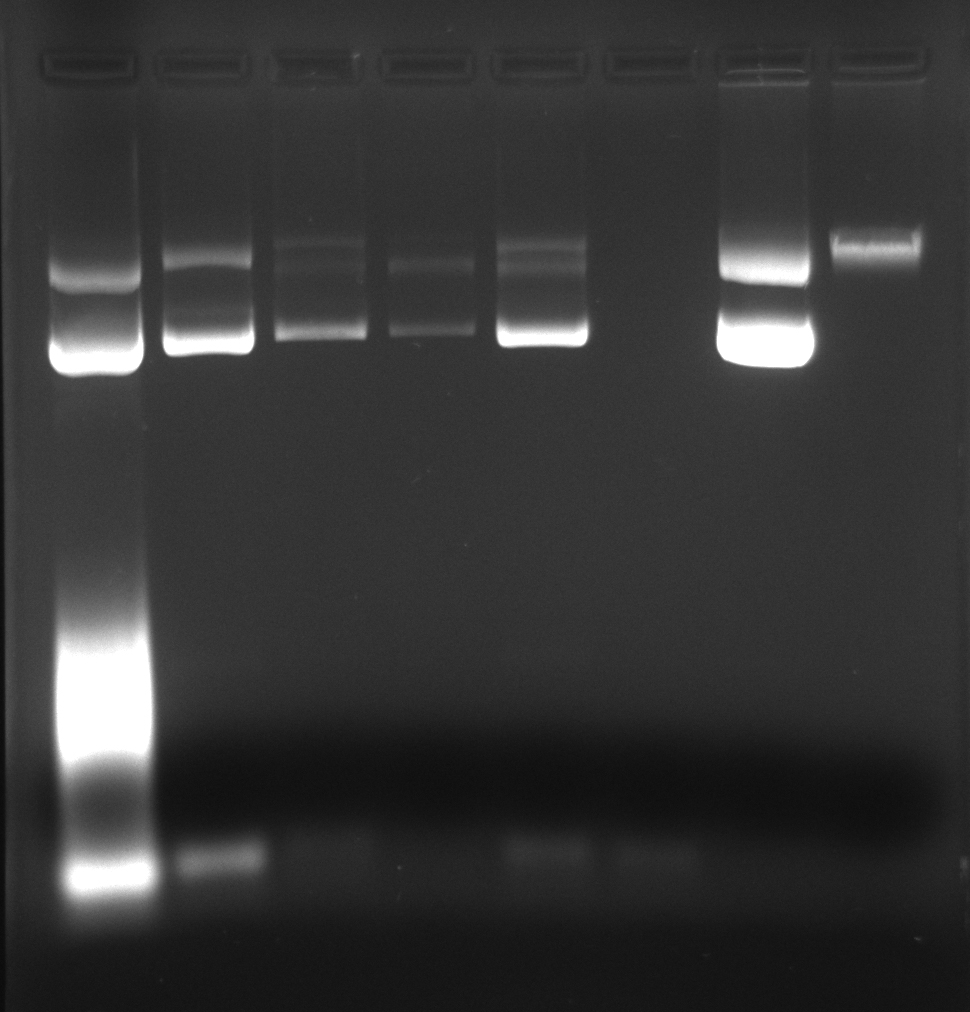
\includegraphics[width=5cm]{ima2}};
\begin{scope}[font=\scriptsize]
\node at (-2.025,2.8) {1};
\node at (-1.45,2.8) {2};
\node at (-0.85,2.8) {3};
\node at (-0.3,2.8) {4};
\node at (0.3,2.8) {5};
\node at (0.85,2.8) {6};
\node at (1.45,2.8) {7};
\node at (2.05,2.8) {8};
%
\draw (2.6,1.35) -- (2.75,1.35) -- (2.85,1.6) -- (3,1.6)  node[right] {gDNA};
\draw (2.6,1.25) -- (3,1.25) node[right] {pDNA (oc)};
\draw (2.6,0.9) -- (3,0.9) node[right] {pDNA (sc)};
\draw (2.6,-1) -- (3,-1) node[right] {RNA HMw};
\draw (2.6,-1.9) -- (3,-1.9) node[right] {RNA LMw};
\end{scope}
\end{tikzpicture}
\caption[Eletroforese horizontal em gel de agarose do processo MF-C/UF-C]{Análise por eletroforese horizontal em gel de agarose (1\%) do processo MF-C/UF-C: (1) lisado antes da adição de \cacldois\ 1\,M; (2) lisado após adição de \cacldois\ 1\,M; (3) permeado da microfiltração; (4) concentrado da microfiltração; (5) concentrado da ultrafiltração; (6) permeado da ultrafiltração; (7) amostra purificada de \pVAX\ pelo kit comercial da Qiagen; (8) Amostra de gDNA de \ecolidh, purificado com o kit da Promega.}
\label{fig:4dart3}
\end{figure}

\subsection{Ensaios de ultrafiltração}
\label{subsec:3p2art3}
\index{ultrafiltração}%
Após concluída a operação de diafiltração sólido/líquido, testou-se uma segunda operação de membranas para concentrar, e ao mesmo tempo, purificar o plasmídeo. Para isso, utilizou-se uma membrana de ultrafiltração com um ``cut-off'' de 100\,kDa, feita de um polímero fluorado, modelo \emph{FS40PP} da \emph{Alpha-Laval}, que tem um poro com um raio de 4.1\,nm \cite{meu1}.
\index{FS40PP}%
A concentração dos permeados provenientes dos testes MF-A, MF-B e MF-C foi efetuada à pressão constante de 1\,bar e a um fator de concentração volumétrico (VCF) de 3.0.
\index{fator!de concentração}%
Estes ensaios são denominados UF-A, UF-B e UF-C.
\index{UF-A|see{ultrafiltração}}%
\index{UF-B|see{ultrafiltração}}%
\index{UF-C|see{ultrafiltração}}%
\index{ultrafiltração!UF-A}%
\index{ultrafiltração!UF-B}%
\index{ultrafiltração!UF-C}%
Obtiveram-se fluxos consideravelmente mais altos nos ensaios UF-C quando comparados com os valores obtidos nos restantes dois ensaios, o que provavelmente se ficou a dever à remoção prévia dos contaminantes hidrofóbicos, tal como se pode verificar na figura~\ref{fig:5aart3}.
\index{contaminantes!hidrofóbicos}%
No entanto, os rendimentos de recuperação mais altos registaram-se nos ensaios UF-A (97$\pm$2\%) como indicado na figura~\ref{fig:5bart3}.
\index{rendimento!de recuperação}%
Nos ensaios UF-B e UF-C, os rendimentos obtidos foram (93$\pm$2\%) e (89$\pm$3\%), respetivamente, tal como se pode verificar na mesma figura. Uma vez que a concentração de pDNA medida nos permeados foi consistentemente muito reduzida para os testes UF-B e UF-C, observaram-se valores significativos de adsorção, $\sim$7 e $\sim$11\% respetivamente.
\index{adsorção!membrana}%
Nos ensaios UF-A verificou-se uma menor ocorrência de adsorção ($\sim$3\%). Observou-se permeação de contaminantes em todos os ensaios de ultrafiltração, o que levou a um significativo grau de purificação, dado que o plasmídeo foi sempre muito retido pela membrana.
\index{contaminantes!hidrofílicos}%
Para o caso dos contaminantes hidrofílicos, a sua remoção corresponde praticamente ao valor teórico considerando permeação total, que é igual a 66\% para um fator de concentração volumétrico de 3.0. Para os contaminantes hidrofóbicos verificou-se uma remoção de $20-40$\porcento, o que indica uma permeação observada de cerca de 0.5. 
\begin{figure}
	\centering
	\setlength\figureheight{6cm} 
	\setlength\figurewidth{6cm}
	% This file was created by matlab2tikz v0.3.3.
% Copyright (c) 2008--2013, Nico Schlömer <nico.schloemer@gmail.com>
% All rights reserved.
% 
% The latest updates can be retrieved from
%   http://www.mathworks.com/matlabcentral/fileexchange/22022-matlab2tikz
% where you can also make suggestions and rate matlab2tikz.
% 
% 
% 
\begin{tikzpicture}

\begin{axis}[%
width=\figurewidth,
height=\figureheight,
scale only axis,
xmin=1,
xmax=3.25,
xlabel={VDF},
ymin=0,
ymax=30,
ylabel={\fluxo\,[\micro\meter/s]},
legend style={at={(1.03,0.5)},anchor=west,draw=black,font=\scriptsize,fill=white,legend cell align=left}
]
\addplot [
color=black,
solid,
mark=*,
mark options={solid,fill=white,draw=black}
]
plot [error bars/.cd, y dir = both, y explicit,error bar style={solid}]
coordinates{
(1.108870968,23.26683292) +- (0.0,2.16957606)(1.245967742,20.57356608) +- (0.0,1.94513716)(1.431451613,18.17955112) +- (0.0,1.64588529)(1.665322581,16.3840399) +- (0.0,1.34663342)(2,14.96259352) +- (0.0,2.09476309)(2.5,13.69077307) +- (0.0,2.01995012)(2.943548387,13.24189526) +- (0.0,1.87032419)};
\addlegendentry{UF-A};

\addplot [
color=black,
dashed,
mark=*,
mark options={solid,fill=black,draw=black}
]
plot [error bars/.cd, y dir = both, y explicit,error bar style={solid}]
coordinates{
(1.112903226,22.81795511) +- (0.0,2.24438903)(1.25,15.11221945) +- (0.0,1.34663342)(1.427419355,11.97007481) +- (0.0,1.12219452)(1.665322581,10.32418953) +- (0.0,0.748129670000001)(2,9.351620948) +- (0.0,0.822942641999999)(2.5,8.753117207) +- (0.0,0.748129676)(3.008064516,8.453865337) +- (0.0,0.748129674999999)};
\addlegendentry{UF-B};

\addplot [
color=black,
dash pattern=on 1pt off 3pt on 3pt off 3pt,
mark=triangle*,
mark options={solid,fill=black,draw=black}
]
plot [error bars/.cd, y dir = both, y explicit,error bar style={solid}]
coordinates{
(1.112903226,24.83790524) +- (0.0,2.16957606)(1.25,23.04239401) +- (0.0,2.24438903)(1.427419355,21.17206983) +- (0.0,1.94513715)(1.665322581,19.52618454) +- (0.0,2.01995012)(2,17.80548628) +- (0.0,1.72069826)(2.504032258,16.3840399) +- (0.0,1.42144638)(3.004032258,15.86034913) +- (0.0,1.42144638)};
\addlegendentry{UF-C};

\end{axis}
\end{tikzpicture}%
	\caption[Fluxo de permeado em função do fator de concentração volumétrico (UF)]{Fluxo de permeado em função do fator de concentração volumétrico (VCF) para os ensaios de ultrafiltração. Condições operatórias: $p=1$\,bar, $\agitacao=760$\,\minmum, $T=25$\,\degreecelsius.}
	\label{fig:5aart3}
\end{figure}
\begin{figure}
\centering
\begin{tikzpicture}
\node[right,font=\scriptsize] at (0,5.75) {Ultrafiltração};
\begin{axis}[
	width=8cm,
	height=6cm,
	scale only axis,
	ybar,
	bar width=5pt,
	ymin=0,
	ymax=1.15,
	enlarge x limits=0.25,
	legend style={at={(0.5,-0.15),font=\scriptsize},
	anchor=north,legend columns=3,legend cell align=left},
	symbolic x coords={UF-A,UF-B,UF-C},
	xtick=data,
	]
\addplot[draw=black,fill=black,
	error bars/.cd,
	y dir=plus,y explicit]
coordinates {
	(UF-A,0.973568282) +- (UF-A,0.015418502)
	(UF-B,0.931718062) +- (UF-B,0.015418502)
	(UF-C,0.894273128) +- (UF-C,0.030837004)};
% Rend pVAX
\addplot[draw=black,fill=gray,
	error bars/.cd,
	y dir=plus,y explicit]
coordinates {
	(UF-A,0.665198238) +- (UF-A,0.030837004)
	(UF-B,0.599118943) +- (UF-B,0.039647577)
	(UF-C,0.698237886) +- (UF-C,0.094713656)};
% Rend Fil
\addplot[draw=black,fill=lightgray,
	error bars/.cd,
	y dir=plus,y explicit]
coordinates {
	(UF-A,0.292951542) +- (UF-A,0.099118943)
	(UF-B,0.213656388) +- (UF-B,0.044052863)
	(UF-C,0.691629956) +- (UF-C,0.052863436)};
% Rend Fob
%Ads pVAX
\addplot[error bars/.cd,
	y dir=plus,y explicit]
coordinates {
	(UF-A,0.022026432) +- (UF-A,0.028634361)
	(UF-B,0.059471366) +- (UF-B,0.024229075)
	(UF-C,0.101321586) +- (UF-C,0.028634361)};
%
\addplot[draw=black,pattern=north west lines,
	error bars/.cd,
	y dir=plus,y explicit]
coordinates {
	(UF-A,0.057268722) +- (UF-A,0.008810573)
	(UF-B,0.072687225) +- (UF-B,0.022026432)
	(UF-C,0.04845815) +- (UF-C,0.024229075)};
%
\addplot[draw=black,pattern=north east lines,
	error bars/.cd,
	y dir=plus,y explicit]
coordinates {
	(UF-A,0.066079295) +- (UF-A,0.011013216)
	(UF-B,0.160792952) +- (UF-B,0.079295154)
	(UF-C,0.303964758) +- (UF-C,0.085903084)};
\legend{Rendimento pDNA,Remoção c. hidrofílicos,Remoção c. hidrofóbicos,Adsorção pDNA,Adsorção c. hidrofílicos, Adsorção c. hidrofóbicos}
\end{axis}
\end{tikzpicture}
\caption[Valores de rendimento, adsorção e remoção (UF)]{Valores experimentais, obtidos nos testes de ultrafiltração, de adsorção e de rendimento de recuperação de pDNA e de adsorção e rendimentos de remoção de contaminantes hidrofílicos e de contaminantes hidrofóbicos.}
\label{fig:5bart3}
\end{figure}
\begin{figure}
\centering
\begin{tikzpicture}
\node at (0,0) {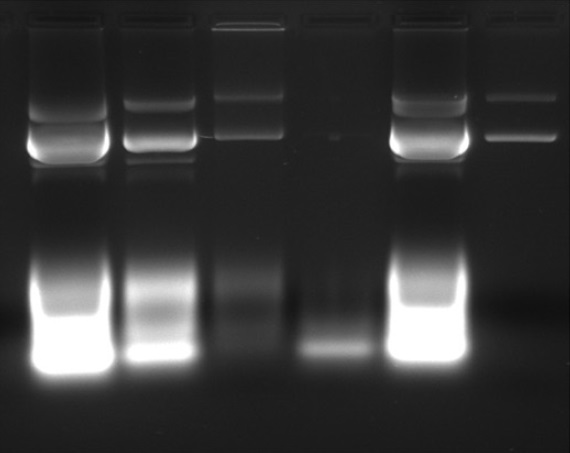
\includegraphics[width=5cm]{ima3}};
\begin{scope}[font=\scriptsize]
\node at (-1.95,2.2) {1};
\node at (-1.15,2.2) {2};
\node at (-0.3,2.2) {3};
\node at (0.45,2.2) {4};
\node at (1.3,2.2) {5};
\node at (2.1,2.2) {6};
\draw (2.6,1.15) -- (3,1.15) node[right] {pDNA (oc)};
\draw (2.6,0.8) -- (3,0.8) node[right] {pDNA (sc)};
\draw (2.6,-0.5) -- (3,-0.5) node[right] {RNA HMw};
\draw (2.6,-1.05) -- (3,-1.05) node[right] {RNA LMw};
\end{scope}
\end{tikzpicture}
\caption[Eletroforese horizontal em gel de agarose do processo MF-A/UF-A]{Análise por eletroforese horizontal em gel de agarose (1\porcento) do processo MF-A/UF-A: (1) Lisado; (2) permeado da microfiltração; (3) concentrado da microfiltração; (4) permeado da ultrafiltração; (5) concentrado da ultrafiltração; (6) amostra purificada de \pVAX.}
\label{fig:5cart3}
\end{figure}

Considerando os valores experimentais de fluxo de permeado, as permeações observadas teóricas para o pDNA, e para as várias espécies de RNA, podem ser estimadas ao longo dos diferentes processos de concentração para interpretar as diferenças entre o comportamento do plasmídeo e dos contaminantes (ver figura~\ref{fig:6art3}). Como se pode observar na figura~\ref{fig:6art3}(a), são esperados valores reduzidos de \permobs, ao longo do processo de ultrafiltração, um resultado que está de acordo com as reduzidas permeações observadas obtidas experimentalmente.
\index{ultrafiltração!permeação observada}%
Na mesma figura é ainda possível verificar que o modelo teórico prevê valores consideravelmente reduzidos de \permobs, quer para o RNA 23\,S quer para o RNA 16\,S. No entanto o mesmo não se verifica para o RNA 5\,S, o que provavelmente explica os valores intermédios de permeação observada de RNA total, como mencionado anteriormente.
\index{RNA!23\,S}%
\index{RNA!16\,S}%
\index{RNA!5\,S}%
Os resultados da análise por eletroforese, mostrados na figura~\ref{fig:5cart3}, confirmam esta ideia. Pode-se observar, na mesma figura, que ambas as isoformas do plasmídeo são retidas pela membrana.
\index{AGE}%
\index{isoforma}%
\begin{figure}
\centering
\begin{tikzpicture}

%FIGURA 6 DO ARTIGO 3

%\draw[help lines] (-4,-4) grid (14,21);
\begin{axis}[%Sobs vs FCv UF-A
	width=5cm,
	height=5cm,
	scale only axis,
	xmin=1,
	xmax=2.5,
	xlabel={VDF},
	ymin=-0.1,
	ymax=1.1,
	ylabel={\permobs},
	at={(0cm,14cm)},
	anchor=south west,
	]
\addplot[
color=black,
solid,
]
table[row sep=crcr]{
1.002184087 0.011655012\\
1.16599064 0.009324009\\
1.423712949 0.006993007\\
1.666146646 0.006993007\\
1.858346334 0.006993007\\
1.987207488 0.006993007\\
2.166302652 0.004662005\\
2.502652106 0.004662005\\
};

\addplot[
color=black,
dashed,
]
table[row sep=crcr]{
1.002184087 0.072261072\\
1.080811232 0.065268065\\
1.242433697 0.058275058\\
1.395319813 0.053613054\\
1.685803432 0.048951049\\
1.976287051 0.044289044\\
2.20124805 0.044289044\\
2.360686427 0.041958042\\
2.500468019 0.03962704\\
};

\addplot [
color=black,
dash pattern=on 1pt off 3pt on 3pt off 3pt,
%forget plot
]
table[row sep=crcr]{
1.002184087 0.146853147\\
1.085179407 0.132867133\\
1.264274571 0.114219114\\
1.458658346 0.102564103\\
1.585335413 0.095571096\\
1.76224649 0.090909091\\
1.939157566 0.086247086\\
2.122620905 0.083916084\\
2.312636505 0.081585082\\
2.500468019 0.079254079\\
};

\addplot [
color=black,
dotted,
%forget plot
]
table[row sep=crcr]{
1.002184087 0.913752914\\
1.133229329 0.883449883\\
1.375663027 0.836829837\\
1.613728549 0.808857809\\
1.808112324 0.79020979\\
2.089859594 0.773892774\\
2.282059282 0.769230769\\
2.502652106 0.764568765\\
};
\end{axis}

\begin{axis}[%Cm/Cb vs FCv UF-A
	width=5cm,
	height=5cm,
	scale only axis,
	xmin=1,
	xmax=2.5,
	xlabel={VDF},
	ymin=0,
	ymax=6,
	ylabel={\concm/\concb},
	at={(7cm,14cm)},
	anchor=south west,
	]
\addplot[
color=black,
solid,
]
table[row sep=crcr]{
1 4.868154158\\
1.06431853 4.430020284\\
1.19295559 3.711967546\\
1.405206738 3.018255578\\
1.540275651 2.738336714\\
1.767534456 2.409736308\\
1.941194487 2.227180527\\
2.166309342 2.093306288\\
2.393568147 1.983772819\\
2.500765697 1.935091278\\
};

\addplot[
color=black,
dashed,
]
table[row sep=crcr]{
1 2.288032454\\
1.098621746 2.068965517\\
1.169372129 1.947261663\\
1.379479326 1.716024341\\
1.617457887 1.569979716\\
1.821133231 1.472616633\\
1.99050536 1.436105477\\
2.11914242 1.39959432\\
2.273506891 1.37525355\\
2.417151608 1.350912779\\
2.502909648 1.338742394\\
};

\addplot [
color=black,
dash pattern=on 1pt off 3pt on 3pt off 3pt,
%forget plot
]
table[row sep=crcr]{
1 2.799188641\\
1.068606432 2.592292089\\
1.197243492 2.288032454\\
1.355895865 2.056795132\\
1.490964778 1.922920892\\
1.692496172 1.764705882\\
1.874732006 1.679513185\\
2.063399694 1.606490872\\
2.192036753 1.582150101\\
2.367840735 1.53346856\\
2.502909648 1.509127789\\
};

\addplot [
color=black,
dotted,
%forget plot
]
table[row sep=crcr]{
1 2.190669371\\
1.092189893 2.14198783\\
1.295865237 2.044624746\\
1.493108729 1.971602434\\
1.619601838 1.947261663\\
1.894027565 1.874239351\\
2.089127106 1.862068966\\
2.241347626 1.84989858\\
2.447166922 1.837728195\\
2.500765697 1.837728195\\
};
\end{axis}

\begin{axis}[%Sobs vs FCv UF-B
	width=5cm,
	height=5cm,
	scale only axis,
	xmin=1,
	xmax=2.5,
	xlabel={VDF},
	ymin=0,
	ymax=1.1,
	ylabel={\permobs},
	at={(0cm,7cm)},
	anchor=south west,
	]
\addplot[
color=black,
solid,
]
table[row sep=crcr]{
1 0.198135198\\
1.045865835 0.160839161\\
1.120124805 0.111888112\\
1.211856474 0.086247086\\
1.351638066 0.067599068\\
1.508892356 0.055944056\\
1.67925117 0.048951049\\
1.821216849 0.044289044\\
1.947893916 0.03962704\\
2.175039002 0.034965035\\
2.356318253 0.032634033\\
2.5 0.03030303\\
};

\addplot[
color=black,
dashed,
]
table[row sep=crcr]{
1 0.475524476\\
1.024024961 0.433566434\\
1.056786271 0.368298368\\
1.102652106 0.298368298\\
1.133229329 0.27039627\\
1.181279251 0.237762238\\
1.290483619 0.202797203\\
1.401872075 0.17948718\\
1.618096724 0.149184149\\
1.840873635 0.132867133\\
1.99375975 0.125874126\\
2.146645866 0.118881119\\
2.288611544 0.114219114\\
2.439313573 0.10955711\\
2.5 0.107226107\\
};

\addplot [
color=black,
dash pattern=on 1pt off 3pt on 3pt off 3pt,
%forget plot
]
table[row sep=crcr]{
1 0.804195804\\
1.028393136 0.724941725\\
1.085179407 0.582750583\\
1.150702028 0.48018648\\
1.224960998 0.417249417\\
1.299219969 0.377622378\\
1.473946958 0.317016317\\
1.655226209 0.284382284\\
1.899843994 0.256410256\\
2.100780031 0.242424242\\
2.277691108 0.233100233\\
2.408736349 0.226107226\\
2.5 0.221445221\\
};

\addplot [
color=black,
dotted,
%forget plot
]
table[row sep=crcr]{
1 0.955710956\\
1.063338534 0.8997669\\
1.133229329 0.850815851\\
1.220592824 0.813519814\\
1.336349454 0.778554779\\
1.528549142 0.750582751\\
1.64648986 0.738927739\\
1.853978159 0.722610723\\
2.081123245 0.715617716\\
2.32574103 0.710955711\\
2.5 0.708624709\\
};
\end{axis}

\begin{axis}[%Cm/Cb vs FCv UF-B
	width=5cm,
	height=5cm,
	scale only axis,
	xmin=1,
	xmax=2.5,
	xlabel={VDF},
	ymin=-5,
	ymax=70,
	ylabel={\concm/\concb},
	at={(7cm,7cm)},
	anchor=south west,
	]
\addplot[
color=black,
solid,
]
table[row sep=crcr]{
1 59.0070922\\
1.023913043 52.19858156\\
1.084782609 38.58156028\\
1.126086957 31.91489362\\
1.180434783 27.23404255\\
1.247826087 23.82978723\\
1.339130435 20.56737589\\
1.484782609 17.0212766\\
1.660869565 14.32624113\\
1.823913043 12.76595745\\
2.013043478 11.34751773\\
2.256521739 10.21276596\\
2.5 9.219858156\\
};

\addplot[
color=black,
dashed,
]
table[row sep=crcr]{
1 15.03546099\\
1.030434783 13.04964539\\
1.07826087 10.4964539\\
1.152173913 8.085106383\\
1.236956522 6.95035461\\
1.317391304 6.241134752\\
1.469565217 5.24822695\\
1.606521739 4.822695035\\
1.752173913 4.397163121\\
1.913043478 4.113475177\\
2.058695652 3.829787234\\
2.204347826 3.687943262\\
2.284782609 3.687943262\\
2.434782609 3.404255319\\
2.5 3.404255319\\
};

\addplot [
color=black,
dash pattern=on 1pt off 3pt on 3pt off 3pt,
%forget plot
]
table[row sep=crcr]{
1 15.31914894\\
1.065217391 11.91489362\\
1.130434783 9.503546099\\
1.197826087 8.226950355\\
1.32173913 6.95035461\\
1.458695652 6.09929078\\
1.639130435 5.390070922\\
1.815217391 4.964539007\\
2.054347826 4.680851064\\
2.263043478 4.397163121\\
2.5 4.255319149\\
};

\addplot [
color=black,
dotted,
%forget plot
]
table[row sep=crcr]{
1 2.269503546\\
1.091304348 2.127659574\\
1.302173913 1.843971631\\
1.608695652 1.70212766\\
1.930434783 1.560283688\\
2.12826087 1.70212766\\
2.367391304 1.560283688\\
2.5 1.560283688\\
};
\end{axis}

\begin{axis}[%Sobs vs FCv UF-C
	width=5cm,
	height=5cm,
	scale only axis,
	xmin=1,
	xmax=2.5,
	xlabel={VDF},
	ymin=0,
	ymax=1.1,
	ylabel={\permobs},
	at={(0cm,0cm)},
	anchor=south west,
	legend style={at={(6cm,-1.5cm)},legend columns=2,anchor=center,font=\scriptsize,draw=black,fill=white,legend cell align=left}
	]
\addplot[
color=black,
solid,
]
table[row sep=crcr]{
1.002184087 0.948837209\\
1.065522621 0.918604651\\
1.334165367 0.802325581\\
1.476131045 0.73255814\\
1.631201248 0.662790698\\
1.821216849 0.597674419\\
1.958814353 0.565116279\\
2.135725429 0.534883721\\
2.336661466 0.509302326\\
2.500468019 0.490697674\\
};
\addlegendentry{\pVAX};

\addplot[
color=black,
dashed,
]
table[row sep=crcr]{
1.002184087 0.979069767\\
1.096099844 0.979069767\\
1.24024961 0.979069767\\
1.386583463 0.979069767\\
1.543837754 0.979069767\\
1.685803432 0.979069767\\
1.987207488 0.979069767\\
2.20124805 0.979069767\\
2.417472699 0.979069767\\
2.5 0.979069767\\
};
\addlegendentry{RNA 23\,S};

\addplot [
color=black,
dash pattern=on 1pt off 3pt on 3pt off 3pt,
%forget plot
]
table[row sep=crcr]{
1.002184087 0.997674419\\
1.159438378 0.993023256\\
1.445553822 0.98372093\\
1.642121685 0.972093023\\
1.816848674 0.960465116\\
2.013416537 0.951162791\\
2.194695788 0.946511628\\
2.428393136 0.941860465\\
2.5 0.941860465\\
};
\addlegendentry{RNA 16\,S};

\addplot [
color=black,
dotted,
%forget plot
]
table[row sep=crcr]{
1.002184087 0.962790698\\
1.172542902 0.946511628\\
1.535101404 0.91627907\\
1.770982839 0.9\\
1.934789392 0.890697674\\
2.120436817 0.88372093\\
2.292979719 0.881395349\\
2.5 0.879069767\\
};
\addlegendentry{RNA 5\,S};
\end{axis}

\begin{axis}[%Cm/Cb vs FCv UF-C
	width=5cm,
	height=5cm,
	scale only axis,
	xmin=1,
	xmax=2.5,
	xlabel={VDF},
	ymin=-10,
	ymax=200,
	ylabel={\concm/\concb},
	at={(7cm,0cm)},
	anchor=south west,
	]
\addplot[
color=black,
solid,
]
table[row sep=crcr]{
1 179.5955056\\
1.112087912 170.2921348\\
1.279120879 156.5393258\\
1.487912088 137.9325843\\
1.668131868 122.5617978\\
1.824175824 112.8539326\\
1.98021978 105.9775281\\
2.107692308 101.9325843\\
2.287912088 97.48314607\\
2.432967033 94.24719101\\
2.5 93.03370787\\
};

\addplot[
color=black,
dashed,
]
table[row sep=crcr]{
1 31.14606742\\
1.171428571 31.14606742\\
1.397802198 31.14606742\\
1.681318681 31.14606742\\
1.905494505 31.14606742\\
2.118681319 31.14606742\\
2.342857143 31.14606742\\
2.5 31.14606742\\
};

\addplot [
color=black,
dash pattern=on 1pt off 3pt on 3pt off 3pt,
%forget plot
]
table[row sep=crcr]{
1 19.01123596\\
1.206593407 18.60674157\\
1.514285714 18.20224719\\
1.810989011 18.20224719\\
2.059340659 17.79775281\\
2.301098901 17.79775281\\
2.5 17.79775281\\
};

\addplot [
color=black,
dotted,
%forget plot
]
table[row sep=crcr]{
1 2.426966292\\
1.217582418 2.02247191\\
1.615384615 2.02247191\\
1.892307692 2.02247191\\
2.206593407 2.02247191\\
2.406593407 2.02247191\\
2.5 2.02247191\\
};
\end{axis}

\begin{scope}[font=\large]
\node[right] at (0,19.5) {a)};
\node[right] at (7,19.5) {b)};
\node[right] at (0,12.5) {c)};
\node[right] at (7,12.5) {d)};
\node[right] at (0,5.5) {e)};
\node[right] at (7,5.5) {f)};
\end{scope}

\begin{scope}[font=\scriptsize]
\node[right] at (0,18.75) {UF-A};
\node[right] at (7,18.75) {UF-A};
\node[right] at (0,11.75) {UF-B};
\node[right] at (7,11.75) {UF-B};
\node[right] at (0,4.75) {UF-C};
\node[right] at (7,4.75) {UF-C};
\end{scope}

\end{tikzpicture}
\caption[Permeação e polarização de concentração previstas em função do fluxo]{Permeação observada e polarização de concentração previstas em função do fluxo, para as espécies indicadas, ao longo dos ensaios de ultrafiltração (UF-A, UF-B e UF-C). Utilizaram-se os modelos CSC e FJC, considerando efeitos de carga, para $\raioporo=4.1$\,nm. Condições: \fluxo\ como indicado na figura~\ref{fig:5aart3}, $\agitacao=760$\,\minmum, $T=25$\,\degreecelsius.}
\label{fig:6art3}
\end{figure}

A polarização de concentração não foi excessiva durante os ensaios UF-A, como se pode observar a partir das simulações representadas na figura~\ref{fig:6art3}(b), o que provavelmente explica a menor adsorção do plasmídeo verificada nestes ensaios.
\index{polarização de concentração}%
Para os outros ensaios, o modelo prevê um aumento da polarização de concentração, devido ao aumento da força iónica, tal como se pode verificar nas figuras~\ref{fig:6art3}(d)~e~(f).
\index{força iónica}%
Uma elevada polarização de concentração pode levar ou a uma maior permeação do plasmídeo (e RNA) ou a uma maior adsorção nos ensaios UF-B e UF-C, quando comparados com os ensaios UF-A. Tal como se pode concluir pela análise dos resultados experimentais, mostrados na figura~\ref{fig:5bart3}, o aumento de polarização de concentração conduziu essencialmente a um aumento do valor da adsorção. Assim, as permeações observadas previstas, indicadas na figura~\ref{fig:6art3}(c)~e~(e), não são corretas devido à ocorrência de adsorção. A elevada tendência do pDNA para se adsorver em membranas, em condições de elevada polarização de concentração, foi previamente identificada no capítulo~\ref{chap:art2}. Foi observada uma elevada permeação de proteínas através da membrana de ultrafiltração, com exceção dos ensaios com o tampão ``B'', tal como se pode observar na tabela~\ref{tab:3art3}. Pela análise de lisados por SEC, discutida no capítulo~\ref{cha:pra}, pode-se concluir que o material proteico presente nos lisados tem uma menor massa molecular que o LMw\,RNA, o que indica que deve permear pela membrana. No caso dos ensaios com o tampão ``B'', a permeação de proteínas deverá ter sido influenciada pelo maior grau de colmatação da membrana, tal como se pode observar na figura~\ref{fig:5aart3}.
\begin{table}%
\caption[Proteína total e DNA genómico (gDNA) nos concentrados (UF)]{Proteína total e DNA genómico (gDNA) nos concentrados dos ensaios de ultrafiltração e os seus rendimentos de remoção (\remocaodois) na operação de ultrafiltração}
\label{tab:3art3}
\centering
\begin{tabular*}{12cm}{lr@{}l @{\extracolsep{\fill}} lll}
\toprule
Tampão &\multicolumn{2}{l}{Proteínas [\micro g/mL]} &  \remocaodois\ (\porcento) & gDNA [\micro g/mL] & \remocaodois (\porcento) \\
\midrule
``A'' & 64 & & 65 & 92 & 28 \\
``B'' & 166 & & 22 & 44 & 20 \\
``C'' & 55 & & 59 & 17 & -5 \\
\bottomrule
\end{tabular*}
\end{table}

Observou-se uma permeação significativa de gDNA para os tampões ``A'' e ``B'', o que indica a presença de fragmentos de gDNA de menores dimensões que o plasmídeo, que por sua vez é retido.
\index{tampão!MF-A}%
\index{tampão!MF-B}%
A maior remoção de gDNA foi verificada nos ensaios UF-A, seguidos dos ensaios UF-B e por fim dos ensaios UF-C, onde não se observou remoção de gDNA. Assim, quando a re-dissolução de gDNA é alta no passo de microfiltração a remoção é igualmente alta no passo de ultrafiltração (ver tabelas~\ref{tab:2art3}~e~\ref{tab:3art3}), o que sugere que a re-dissolução do gDNA é provocada pela quebra das cadeias.
\index{DNA genómico!redissolução}%
A partir dos dados de remoção de gDNA obtidos nos ensaios UF-A e UF-B (indicados na tabela~\ref{tab:3art3}) a massa molecular média dos fragmentos de gDNA que chegam à operação de ultrafiltração pode ser estimada como descrito em \cite{meu3}.
\index{DNA genómico!fragmentos}%
Considerando que estes fragmentos são compostos por DNA linear de dupla cadeia (dsDNA) o número de pares de bases deverá ser, de acordo com os cálculos efetuados em \cite{meu3}, 205 no caso do tampão ``A'' e 1700 no caso do tampão ``B''. Estes valores correspondem a raios hidrodinâmicos de 16\,nm e 59\,nm, respetivamente, o que indica que estes fragmentos são consideravelmente menores que o plasmídeo usado, cujo raio hidrodinâmico é de 83\,nm. Pode-se assim concluir que apesar do gDNA se re-dissolver no passo de microfiltração, os fragmentos resultantes podem ser removidos no passo de ultrafiltração. O grau de remoção pode ser assim melhorado com recurso a uma diafiltração neste segundo passo, uma vez que o plasmídeo é retido pela membrana. No entanto, e em especial para o caso do RNA de alto peso molecular (HMw\,RNA), não é esperado que se venham a obter rendimentos de remoção muito elevados, dado os reduzidos valores verificados da permeação desta biomolécula. No capítulo~\ref{chap:art4} a separação pDNA/RNA é estudada em melhor detalhe.

\section{Conclusões}
Os modelos teóricos desenvolvidos de transferência de massa para cadeias CSC e FJC, usados para prever a permeação de pDNA e RNA na microfiltração de lisados, e subsequente concentração, foram aplicados com sucesso, uma vez que os resultados obtidos nos dois passos de membranas podem ser explicados com base neste desenvolvimento teórico.

A recuperação de um plasmídeo com 6050\,bp, a partir de lisados, foi efetuada de forma eficiente por uma operação de microfiltração, usando uma membrana hidrofílica de Nylon, com um tamanho de poro nominal de 0.2\,\micro m. Este tamanho de poro, bem como as condições operacionais, foi selecionado com base nas previsões teóricas para que se evite, quer uma excessiva polarização de concentração do plasmídeo, quer a adsorção do mesmo na superfície da membrana. Verificou-se que outros contaminantes, nomeadamente RNA, proteínas e gDNA, permeiam através da membrana de microfiltração juntamente com o plasmídeo. A adição de \cacldois\ 1\,M aos lisados conduziu à remoção quase completa do RNA, tal como esperado pelos resultados encontrados na literatura. Verificou-se igualmente que a adição deste sal reduziu significativamente o conteúdo de gDNA nos lisados, gDNA esse que tende a se re-dissolver durante a operação de microfiltração, o que se observou em todos os ensaios. Um aumento da força iónica da solução de diafiltração pode reduzir esta tendência, no entanto não a elimina por completo.

Estudou-se uma operação de ultrafiltração para purificar e concentrar o plasmídeo após a microfiltração. Apesar do RNA de alto peso molecular ser completamente retido pela membrana, observou-se alguma permeação de RNA de baixo peso molecular, tal como previsto pelo modelo. Proteínas e gDNA podem ser consideravelmente removidos por ultrafiltração. A elevada permeabilidade dos fragmentos de gDNA na operação de ultrafiltração pode ser explicada pelos seus reduzidos tamanhos, que se estimou serem consideravelmente inferiores ao plasmídeo usado. Assim, apesar de se verificar uma significativa re-dissolução de gDNA no passo de microfiltração, os fragmentos presentes em solução são de tamanho reduzido e podem ser separados do plasmídeo num passo de ultrafiltração.

%!TEX root=tese.tex
\chapter{Modelação e aplicação prática da separação pDNA/RNA por ultrafiltração}
\label{chap:art4}

\section{Introdução}
\label{sec:art4_intro}
Como referido no capítulo~\ref{chap:intro}, na última década tem sido efetuado um enorme esforço de investigação na área da recuperação e purificação de DNA plasmídico (pDNA) a partir de caldos de fermentação, com o objetivo de facilitar a sua produção em larga-escala, para aplicações em terapia génica e para a formulação de vacinas de DNA \cite{prather,carnes,meu2}. Os processos de separação com membranas estão presentes em praticamente todas as áreas da biotecnologia, numa grande variedade de aplicações \cite{rathore,reis}, e revelam o mesmo potencial de aplicação em processos de produção de DNA plasmídico \cite{carnes,prather,flowsheets}.

A recuperação e posterior purificação de pDNA a partir de caldos de fermentação, que pode ser efetuada por variadas técnicas, tipicamente envolve um passo de lise celular seguido por uma operação de separação sólido-líquido, subsequente precipitação de pDNA com álcoois tais como etanol ou isopropanol (ou mesmo outros agentes precipitantes), ressuspensão do concentrado de pDNA e sua posterior separação de RNA e outros contaminantes por técnicas de adsorção, que tipicamente são técnicas cromatográficas.
\index{caldos de fermentação}%
Estas técnicas cromatográficas são igualmente necessárias, num grande número de esquemas de purificação, para obter a isoforma super-enrolada do plasmídeo, pDNA(sc), com os requisitos de qualidade do produto final, impostos pelas entidades reguladoras, tais como a FDA (U.S.\ Food and Drug Administration) e a EMA (``European Medicines Agency'') \cite{prather,carnes,sousabab}.
\index{isoforma!super-enrolada}%
\index{EMA}%
\index{FDA}%

Operações de membranas foram utilizadas com sucesso para obter a colheita de células, a partir de caldos de fermentação, não só em processos de produção de pDNA como também em processos similares que envolvem suspensões celulares \cite{prather,riesmeier,morao01,brites} e igualmente para a seletiva retenção de detritos celulares, resultantes do processo de lise, permitindo a permeação de moléculas de pDNA \cite{duvaltff,meu3,freitas}. Estas operações foram já igualmente utilizadas na concentração de pDNA, com simultânea troca de tampão e remoção de micro-solutos, a seguir a operações de purificação cromatográfica, assim como para a esterilização do produto final \cite{prather,kong06,kong10}. Para além destas aplicações, as operações de membranas podem ser uma alternativa viável na fase da concentração e pré-purificação do pDNA antes da cromatografia, substituindo o uso de solventes e outros agentes precipitantes. 

A aplicação da ultrafiltração para efetuar a separação entre pDNA e RNA, assim como outros contaminantes, tem vindo a ser estudada por vários autores independentes. Kendall \et\ \cite{kendall} estudaram a purificação de pDNA através da adsorção seletiva de contaminantes em membranas de nitrocelulose.
\index{membrana!nitrocelulose}%
O procedimento desenvolvido permitiu remover quantidades significativas de RNA, DNA genómico e outros contaminantes hidrofóbicos.
\index{DNA genómico}%
No entanto, os problemas relacionados com a colmatação e a reduzida capacidade de membranas para atuarem como materiais adsorventes, podem ser sérias limitações da aplicação prática deste método. Eon-Duvall \et\ \cite{duvaltff} adicionaram cloreto de cálcio aos lisados e efetuaram uma subsequente operação de ultrafiltração para obter uma quase completa remoção de RNA.
\index{cloreto de cálcio!precipitação RNA}%
O facto de ser necessário utilizar uma elevada quantidade de \tce{CaCl2} é assim uma desvantagem do método. Kahn \et\ \cite{kahn} estudaram a aplicação da ultrafiltração de diferentes plasmídeos para obter a concentração de pDNA, e a sua separação do RNA, após um processo modificado de lise alcalina.
\index{lise alcalina!método modificado}%
Este método contempla um aumento do tempo de incubação (24 horas) durante a lise para obter uma degradação do RNA presente e assim obter elevados graus de purificação de pDNA com uma única operação de ultrafiltração. No entanto, o processo desenvolvido tem a desvantagem de conter elevados tempos de incubação para ser possível efetuar a separação, e não é claro que o pDNA não possa igualmente sofrer alguma degradação nestas condições. Freitas \et\ \cite{freitas} utilizaram um processo de ultrafiltração para efetuar uma recuperação intermediária de pDNA antes de um passo final de purificação. Apesar de obterem rendimentos de recuperação de pDNA elevados, o rendimento de remoção de RNA revelou-se ser modesto. 

Tendo em conta o estudo prévio, descrito no capítulo anterior, neste capítulo é investigada a possibilidade de otimizar a operação de ultrafiltração, procurando obter uma elevada retenção de pDNA e uma permeação alta dos principais contaminantes, com especial enfoque no RNA. A purificação de dois plasmídeos diferentes, \pVAX\ e \pCAMBIA, com 6050\,bp e 12361\,bp respetivamente, usando duas membranas de ultrafiltração distintas, é estudada numa célula de filtração agitada.
\index{pVAX@\pVAX}%
\index{pCAMBIA@\pCAMBIA}%
Os efeitos do tamanho do poro das membranas, da velocidade de agitação e do fluxo de filtração na separação entre pDNA e RNA, bem como no grau de colmatação das membranas, são interpretados com base no modelo desenvolvido para a permeação de macrosolutos flexíveis em membranas com poros de menores dimensões (capítulos~\ref{chap:art1}--\ref{chap:art3}). Para obter um termo comparativo, é avaliada a performance de um processo de isolamento intermediário alternativo, com base em duas operações de precipitação seletiva, usado com regularidade em laboratório e com o qual se obtêm resultados satisfatórios no âmbito do isolamento intermediário de pDNA \cite{sousabab,freitas}. 

\section{Materiais e métodos} % (fold)
\label{sec:art4_materias}
\subsection{Produção de pDNA e lise celular} % (fold)
\label{ssub:art4_lise}
Bactérias \emph{E. coli} DH5$\alpha$, contendo um plasmídeo de 6050\,bp (\pVAX), e bactérias \emph{E. coli} XL1\,blue, contendo um plasmídeo de 12361\,bp (\pCAMBIA) foram produzidas por fermentação, usando as mesmas condições de crescimento descritas em \cite{asousa}.
\index{ecolidh@\ecolidh}%
\index{ecolix@\emph{E. coli} XL1\,blue}%
\index{fermentação}%
As bactérias com o plasmídeo \pVAX\ foram cultivadas no meio Terrifc broth (12\,g/L de triptona (\emph{Sigma}), 24\,g/L de extrato de leveduras (\emph{Fluka}), 4\,mL/L de glicerol (\emph{Himedia}), 0.017\,M de \tce{KH2PO4} (\emph{Panreac}) e 0.072\,M de \tce{K2HPO4} (\emph{Panreac}), e as bactérias contendo o plasmídeo \pCAMBIA\ cultivadas em meio Luria Bertani (10\,g/L de triptona, 5\,g/L de extrato de leveduras, 10\,g/L de NaCl (\emph{Panreac}), pH 7.00).
\index{Terrific broth}%
\index{Luria Bertani}%
A lise celular foi obtida por um método modificado de lise alcalina, originalmente desenvolvido por Birnboim e Doly \cite{birnboim}.
\index{lise alcalina!procedimento}%
Resumidamente, a 4\,mL de uma suspensão de bactárias a 120\,g/L (peso húmido), em tampão $\mr{T}_{50}\mr{E}_{10}$ (50\,mM Tris (\emph{Fisher BioReagents}) e 10\,mM EDTA (\emph{Sigma}), pH 8.00), foram adicionados 4\,mL de uma solução de 0.2\,M de NaOH (\emph{Panreac}) e 1\% SDS (\emph{Himedia}). Após 5\,min de incubação a temperatura ambiente, foram adicionados 4\,mL de uma solução previamente arrefecida (4\degreecelsius) de 3\,M de acetato de potássio (\emph{Sigma-Aldrich}) a pH 5.00, com o pH ajustado com ácido acético (\emph{Panreac}). Após agitação suave, a suspensão obtida foi incubada em gelo durante 15\,min antes de ser processada por microfiltração.  
% subsubsection art4_lise (end)

\subsection{Clarificação de lisados - Microfiltração} % (fold)
\label{ssub:2.2art4}
\index{lisado!clarificação}%
O lisado alcalino obtido, contendo uma grande quantidade de sólidos em suspensão, foi filtrado por microfiltração usando uma membrana hidrofílica de Nylon (Nylaflo, \emph{Pall}), com um tamanho de poro nominal de 0.2\,\micro\meter.
\index{Nylon}%
\index{Nylaflo|see{Nylon}}%
Foi efetuada uma diafiltração continua numa célula de filtração agitada, com geometria ``dead-end'', com 50\,mL de capacidade (modelo 8050, \emph{Millipore}).
\index{Amicon 8050}%
A velocidade de agitação foi mantida a 100\,\minmum\ e o caudal de permeado ajustado, e mantido, em 1\,mL/min através de uma bomba peristáltica (modelo 403U/VM2, \emph{Watson Marlow}) colocada a jusante da membrana, operando assim por sucção.
\index{caudal volumétrico}%
\index{velocidade de agitação}%
\index{bomba peristáltica}%
O volume de lisado processado em cada ensaio foi de 10\,mL. O volume da suspensão no interior da célula de filtração foi mantido constante através da contínua adição de Tris/HCl 10\,mM a pH 8.00 (tampão Tris), que foi alimentado à célula de filtração através de uma segunda bomba peristáltica (modelo 101U/R, \emph{Watson Marlow}), ao mesmo caudal.
\index{Tris}%
A filtração foi concluída após a recolha de um total de 30\,mL de permeado. Nestas condições espera-se um rendimento de recuperação de plasmídeo no permeado de cerca de 95\%, considerando que o plasmídeo não é retido pela membrana, fazendo uso da equação do balanço de massa para o modo de diafiltração a volume constante (equação~\ref{bal_mas_df_final}, capítulo~\ref{cha:pra}).
\index{DNA plasmídico!rendimento de recuperação}%
\index{rendimento!de recuperação}%
% subsubsection 2.2art4 (end)

\subsection{Ultrafiltração} % (fold)
\label{ssub:2.3art4}
\index{ultrafiltração}%
Os ensaios de ultrafiltração foram efetuados numa célula de filtração Amicon 8010, com geometria ``dead-end'' (\emph{Millipore}).
\index{Amicon 8010}%
Em todos os ensaios, o volume inicial de lisado alcalino microfiltrado foi de 10\,mL, tendo-se recolhido 9\,mL de permeado, o que equivale a um fator de concentração volumétrico (VCF) igual a 10.
\index{fator!de concentração}%
Testaram-se duas membranas distintas: uma membrana de 100\,kDa de ``cut-off'' de polímero fluorado (FS40PP, \emph{DSS/Alfa-laval}) e uma membrana de 300\,kDa de ``cut-off'' de polietersulfona (Biomax\,300, \emph{Millipore}).
\index{FS40PP}%
\index{Biomax 300}%
\index{PVDF}%
\index{polietersulfona}%
Estas membranas foram previamente caracterizadas, em relação ao tamanho de poro, através do modelo de poros simétricos (SPM) desenvolvido por Morão \et\ \cite{moraompa}.
\index{modelo!dos poros simétricos}%
O caudal de permeado foi mantido constante através do uso de uma bomba peristáltica (modelo 101U/R, \emph{Watson Marlow}), colocada a jusante da membrana. A velocidade de agitação foi ajustada a 100 ou a 760\,\minmum, com calibração prévia.
\index{caudal de permeado}%   
% subsubsection 2.3art4 (end)

\subsection{Isolamento intermediário usando tecnologias de membranas} % (fold)
\label{sub:isol_mem_final}
\index{isolamento intermediário}%
Foram efetuados três conjuntos de ensaios, para o isolamento intermediário de pDNA, com o objetivo de melhorar os valores de remoção de RNA, recorrendo a uma operação de diafiltração. Os ensaios foram todos efetuados em triplicado, tendo-se obtido uma boa reprodutibilidade entre os mesmos. O esquema dos ensaios efetuados, bem como as principais condições operatórias utilizadas, estão representados na figura~\ref{fig:processos_art4} e tabela~\ref{tab:cond_isolamento_art4}, respetivamente. As experiências foram conduzidas numa célula de filtração agitada, com 10 mL de capacidade, com geometria ``dead-end'' (Amicon 8010, \emph{Millipore}). A agitação foi mantida a 760\,\minmum\ em todos os ensaios. O caudal de permeado foi imposto através de uma bomba peristáltica (WM101U/R, \emph{Watson Marlow}). Foram usadas novamente as membranas FS40PP e Biomax\,300. Antes de se iniciar a filtração, as membranas foram lavadas com a filtração de pelo menos 30\,mL de água MilliQ (\emph{Millipore}). Após lavagem das membranas, as suas permeabilidades hidráulicas foram medidas através da determinação do fluxo de água em função da pressão transmembranar, pressão esta imposta pela ligação da célula de filtração a uma garrafa de azoto pressurizado. Foram colocados inicialmente na célula 10 mL de permeado proveniente da microfiltração do lisado. O permeado foi concentrado a um fator de concentração volumétrico (VCF) predefinido (ver tabela~\ref{tab:cond_isolamento_art4}), segundo o método descrito na secção~\ref{ssub:2.3art4}. Após concluída a concentração, foi efetuada uma diafiltração com aproximadamente 4 volumes de diafiltração ($V_{\mr{DF}}$) de Tris/HCl 10 mM a pH 8.00 (tampão Tris), ao mesmo caudal, e utilizando uma segunda bomba peristáltica (WM403U/R, \emph{Watson Marlow}).
\index{diafiltração}%
Foram recolhidas amostras da solução inicial antes da concentração (permeado da microfiltração), do concentrado após diafiltração e do permeado conjunto da fase de concentração e da fase de diafiltração, para posterior análise. Para aferir o grau de colmatação irreversível das membranas usadas, no fim dos ensaios a célula foi lavada com água MilliQ, com agitação suave e breve, e a permeabilidade hidráulica novamente determinada.
% subsection isol_mem_final (end)

\begin{figure}
\centering
	\begin{tikzpicture}

\node[anchor = south west] at (0cm, 0cm) {%\includegraphics[width=7cm]{% mudar para 6.3 cm
\includegraphics[width=14cm]{processos_art4.jpg}};

% \draw[help lines] (0cm, -2cm) grid (14cm, 10cm);

\node[align = center] at (1.5, 4.5) {Filtração lisado \\ (Microfiltração)};
\node[align = center] at (4.5, 4.5) {Concentração \\ (Ultrafiltração)};
\node[align = center] at (7.4, 4.5) {Diafiltração \\ (Ultrafiltração)};

\node[align = center] at (1.5, -0.5) {Centrifugação \\ lisado};
\node[align = center] at (4.4, -0.5) {Precipitação \\ isopropanol};
\node[align = center] at (7.4, -0.5) {Centrifugação \\ \phantom{phantom}};
\node[align = center] at (10.3, -0.5) {Precipitação \\ sulfato de amónio};
\node[align = center] at (13.3, -0.5) {Centrifugação \\ \phantom{phantom}};

\draw[dashed] (3, 4) rectangle (8.9, 7.4);
\draw[dashed] (3, -1) rectangle (14.5, 3.5);

\node[right, align = left] at (9, 6.7) {Processo A:\\FS40PP (\pVAX)};
\node[right, align = left] at (9, 5.7) {Processo B:\\Biomax\,300 (\pVAX)};
\node[right, align = left] at (9, 4.7) {Processo C:\\Biomax\,300 (\pCAMBIA)};
\node at (9.25, -1.5) {Processo D: processo alternativo};

\end{tikzpicture}
	\caption[Esquemas dos processos de isolamento intermediário estudados]{Esquema dos processos estudados de isolamento intermediário de pDNA. A tracejado encontram-se as operações consideradas nos cálculos. Os processos A--C usam exclusivamente operações de membranas. O processo D consiste no procedimento de isolamento intermediário alternativo, descrito em \cite{sousabab}. As condições operatórias para os processos A--C estão especificadas na tabela~\ref{tab:cond_isolamento_art4}.}
	\label{fig:processos_art4}  
\end{figure}
%
\begin{table}[!b]
	\caption[Condições operatórias utilizadas nos ensaios de isolamento intermediário.]{Condições operatórias, utilizadas nos processos com base em tecnologias de membrana, para efetuar o isolamento intermediário de pDNA.}
	\label{tab:cond_isolamento_art4}
\begin{tabular*}{\textwidth}{l@{\extracolsep{\fill}}l l d{9} d{5} d{2} d{6}}
 \toprule
Processo & Membrana & pDNA & \mc{1}{l}{\fluxo$\times 10^{6}$\,[m/s]} & \mc{1}{l}{\agitacao\,[\minmum]} & \mc{1}{l}{VCF} & \mc{1}{l}{$V_{\mr{DF}}$\,[mL]} \\
\midrule
``A'' & FS40PP & \pVAX & 4,2 & 760 & 8 & 3,8 \\
``B'' & Biomax\,300 & \pVAX & 2,4 & 760 & 8,4 & 4 \\
``C'' & Biomax\,300 & \pCAMBIA & 2,4 & 760 & 8,4 & 4 \\
\bottomrule
\end{tabular*}
\end{table}

\subsection{Isolamento intermediário alternativo} % (fold)
\label{sub:isol_alter_final}
\index{isolamento intermediário alternativo}%
Para se obter um termo comparativo, em relação aos resultados obtidos com os ensaios de ultrafiltração/diafiltração, foi igualmente estudado um processo de isolamento intermediário alternativo (Processo D, figura~\ref{fig:processos_art4}), regularmente usado em laboratório \cite{sousabab,freitas}. Foi efetuado o procedimento descrito em \cite{sousabab}. O lisado, proveniente da lise alcalina, foi centrifugado duas vezes a 19\,000\,g, durante 30\,min e a 4\degreecelsius, numa centrífuga Allegra 25R (\emph{Beckman Coulter}).
\index{centrifugação}%
Ao sobrenadante obtido (8\,mL) foram adicionados 0.7 volumes de isopropanol (\emph{Fischer}).
\index{isopropanol!isolamento intermediário alternativo}%
Após 30\,min de incubação em gelo, a suspensão foi centrifugada durante 30\,min, a 16\,000\,g e 4\degreecelsius, na mesma centrífuga. Após remoção do sobrenadante, o ``pellet'' foi dissolvido em 2.5\,mL de tampão Tris. Foi adicionado sulfato de amónio (\emph{Prolabo, VWR}) até perfazer uma concentração de 2.5\,M.
\index{sulfato de amónio!isolamento intermediário alternativo}%
Após incubação durante 15 min em gelo, a suspensão foi centrifugada a 16\,000\,g, durante 20\,min e 4\degreecelsius, numa centrífuga Mikro 200R (\emph{Hettich}). Foram recolhidas amostras ao longo do processo para posterior análise.

\subsection{Parte analítica} % (fold)
\label{ssub:2.4art4}
\subsubsection{Quantificação de pDNA e RNA}
\label{ssubsub:2.4.1art4}
\index{HIC}%
\index{plasmídeo|see{DNA plasmídico}}%
A concentração de plasmídeo nas várias amostras foi determinada pelo método desenvolvido por Diogo \et\ \cite{diogo}. Resumidamente, uma coluna HIC \emph{source 15} PHE, da \emph{Amersham Biosciences (GE Healthcare)} foi conectada a um sistema de FPLC (\emph{Äkta purifier}) da \emph{GE Healthcare}.
\index{akta@Äkta}%
A coluna foi inicialmente equilibrada com 1.5\,M de \tce{(NH4)2SO4} em tampão tris. As amostras (20\,\micro L) foram injetadas e eluídas a um caudal constante de 1\,mL/min. Ao fim de 2\,min após a injeção, o eluente foi instantaneamente mudado para tampão Tris para eluir as espécies adsorvidas. Este tampão foi mantido por mais 4\,min antes de se re-equilibrar a coluna para a preparar para a próxima injeção. A absorvância do eluído foi registada a 260\,nm. A concentração de pDNA em cada amostra foi calculada por intermédio de uma reta de calibração, preparada com padrões de pDNA obtidos com um kit de purificação (\emph{Maxi kit, Qiagen}). Este método está descrito em detalhe no capítulo~\ref{cha:pra}, onde se propõe que a concentração de RNA pode igualmente ser estimada.    
% subsubsection 2.4art4 (end)

\subsubsection{Eletroforese em gel de agarose} % (fold)
\label{ssub:2p4p1art4}
\index{AGE!procedimento}%
As amostras foram analisadas por eletroforese horizontal, em gel de 1.0\% de agarose (\emph{Grisp}), preparado em tampão TAE (40\,mM Tris, 20\,mM ácido acético e 1\,mM de EDTA, pH 8.00), complementado com o corante \emph{GreenSafe} (\emph{NZYTech}).
\index{greensafe@\emph{GreenSafe}}%
As análises decorreram a 110\,V, durante 40\,min, numa célula da \emph{BioRad}. Os géis foram visualizados num transiluminador da \emph{Uvitec}, modelo \emph{Essential V2}.
\index{transiluminador}%
Para concentrar, e/ou evitar possíveis interferências provocadas pelos sais presentes, algumas amostras foram dessalinizadas, através de precipitação com isopropanol, tal como descrito no capítulo~\ref{chap:art3}.
\index{isopropanol!dessalinização}%
% subsubsection 2p4p1art4 (end)

\subsection{Simulações} % (fold)
\label{sub:2p5art4}
Para efetuar uma otimização da operação de ultrafiltração, com o intuito de obter uma elevada retenção de pDNA e uma elevada permeação de RNA, efetuaram-se simulações, quer para um sistema de 3 componentes contendo a macromolécula de interesse (pDNA ou RNA, componente 1), ião acetato (componente 2) e ião potássio (componente 3), quer para um sistema de 4 componentes contendo o plasmídeo, uma espécie de RNA (23S, 16S ou 5S), o ião acetato e o ião potássio.
\index{modelo!3 componentes}%
\index{modelo!4 componentes}%
Nas simulações utilizou-se o método descrito nos capítulos~\ref{chap:teov3}, \ref{chap:art2} e \ref{chap:art3}. Apesar de nos lisados microfiltrados existirem outros sais presentes em solução, os iões \tce{CH3COO-} e \tce{K+} são, por larga margem, os que se encontram em maior quantidade, sendo os principais responsáveis pelos efeitos de carga que afetam em grande medida a polarização de concentração de macrosolutos (pDNA e RNA) que são altamente carregados negativamente.
\index{iao@ião!potássio}%
\index{iao@ião!acetato}%

O modelo de transferência de massa anteriormente desenvolvido permite estimar a permeação de macrosolutos em membranas com poros de reduzidas dimensões, ou seja, poros com um raio médio inferior ao raio de giração do macrosoluto, sendo que este último deverá apresentar alguma flexibilidade. Este modelo foi originalmente desenvolvido para moléculas lineares, que foram modeladas como cadeias de ligação livre (FJC), nomeadamente para pDNA linear e para polissacáridos lineares (capítulo~\ref{chap:art1}). O modelo foi estendido ao caso de macrosolutos de cadeia fechada, através da sua representação pelo modelo de cadeias fechadas segmentadas (CSC), discutido nos capítulos~\ref{chap:teov3}~e~\ref{chap:art2}. De facto, verificou-se que a equação obtida, que relaciona o rácio entre o raio de giração da molécula e o raio do poro com o coeficiente de partição, pode ser usada quer para cadeias FJC quer para cadeias CSC (capítulo~\ref{chap:art2}). Apesar de uma molécula de pDNA poder ser modelada como uma FJC, a representação CSC é, aparentemente, uma melhor aproximação por permitir obter valores de raio de giração em melhor concordância com os valores encontrados na literatura. O modelo desenvolvido pode igualmente ser usado para prever a permeação de RNA, considerando-o uma molécula linear, ou seja, utilizando o modelo FJC, tal como indicado no capítulo~\ref{chap:art3}, onde se aplicou o modelo de 3 componentes para prever a permeação das principais espécies de RNA presentes nos lisados, nomeadamente os RNA's 23S, 16S e 5S, de forma individual. 

Neste capítulo investiga-se a possível mútua interferência entre pDNA e RNA nas suas permeações, considerando um sistema de 4 componentes. A inclusão de um maior número de componentes no modelo representa uma interpretação mais realista do fenómeno mas aumenta consideravelmente a complexidade dos cálculos e o esforço computacional necessário. Para além disso, tal como mostrado mais à frente, a principal interferência é o efeito do pDNA na permeação do RNA e não o contrário, sendo que este último efeito pode ser simulado com um sistema de 4 componentes. 

As simulações do processo de ultrafiltração foram levadas a cabo considerando um cenário de filtração numa célula agitada, com 10\,mL de solução inicial (permeado da microfiltração), em condições de fluxo e velocidade de agitação constantes e em modo de concentração, cenário este consistente com o procedimento experimental descrito na secção~\ref{ssub:2.3art4}. As concentrações inicias das macromoléculas e sais usados nas simulações, assim como as suas propriedades mais relevantes, estão indicadas na tabela~\ref{tab:1art4}. As várias propriedades das moléculas foram determinadas pelos métodos discutidos na secção~\ref{sec:solutos}. 
\begin{table}
	\caption[Componentes e suas propriedades relevantes]{Principais componentes do lisado microfiltrado e as suas propriedades mais relevantes para fins de modelação.}
	\label{tab:1art4}
\begin{threeparttable}
\begin{tabular*}{15cm}{l@{\extracolsep{\fill}} l d{0} d{6} d{6} d{8} }
\toprule
Componente\phantom{MM}&\concb\,[mol/$\mr{m}^3$]&\mc{1}{r}{M$\mr{_w}$\,[Da]\phantom{l}}&\mc{1}{l}{$\raiostokes\times 10^9$\,[m]}&\mc{1}{l}{$\raiogiracao\times 10^9$\,[m]} & \mc{1}{l}{$D\times 10^{12}\,[\mr{m}^2/\mr{s}]$}\\
\midrule
\tce{CH3COO-} & $3.17\times 10^2$ & 59 & 0,227 &  & 1089\\
\tce{K+}	     & $3.17\times 10^2$ & 39 & 0,125 &  & 1950 \\
RNA 5S              & $2.26\times 10^{-3}$\tnote{a} & 40800 & 3,39 & 5,10 & 72,9\tnote{c}\\
                          & $8.45\times 10^{-4}$\tnote{b} &            &         &          &            \\
RNA 16S            & $1.06\times 10^{-4}$\tnote{a} & 523940 & 13,6 & 20,5 & 18,2\tnote{c}\\ 
                          & $8.99\times 10^{-5}$\tnote{b} &              &          &         &           \\
RNA 23S            & $5.63\times 10^{-5}$\tnote{a} & 987360& 17,8 & 26,8 &  13,9\tnote{c} \\
                          & $4.77\times 10^{-5}$\tnote{b} &             &         &         &           \\
\pVAX                 & $4.47\times 10^{-6}$\tnote{a} & 3993000 & 83,1 & 87,3 & 2,97\tnote{d}\\
\pCAMBIA                          & $6.39\times 10^{-7}$\tnote{b} & 8158260 & 134 & 138,7 & 1,85 \tnote{d}\\
\bottomrule
\end{tabular*}
\begin{tablenotes}
\item[a] Lisados provenientes da produção de \pVAX  
\item[b] Lisados provenientes da produção de \pCAMBIA
\item[c] Valores obtidos no capítulo~\ref{chap:art3}
\item[d] Valores obtidos em \cite{prazeresdif}
\end{tablenotes}
\end{threeparttable}
\end{table}
% subsection 2p5art4 (end)
% section art4_materias (end)

\section{Resultados e discussão} % (fold)
\label{sec:3art4}
\subsection{Simulações} % (fold)
\label{sub:3.1art4}
Para proceder à otimização de uma operação de ultrafiltração, com o objetivo de concentrar o pDNA e simultâneamente proceder à sua separação do RNA presente, o raio do poro da membrana, \raioporo, e o fluxo de filtração, \fluxo, devem ser os primeiros parâmetros a considerar. Em seguida, deve-se testar o material da membrana, nomeadamente em termos da sua suscetibilidade à colmatação e adsorção de plasmídeo, que deve ser o mais reduzida possível. Assim, os efeitos de \raioporo\ e \fluxo\ nas permeações das moléculas indicadas na tabela~\ref{tab:1art4} foram estimados antes dos ensaios experimentais. As previsões foram efetuadas considerando quer o modelo de 3 componentes, quer o modelo de 4 componentes, descritos na secção~\ref{sub:2p5art4}, em condições ideais de ausência de colmatação e adsorção de pDNA e RNA.

O efeito previsto das diferentes moléculas de RNA na permeação observada, \permobs, do plasmídeo \pVAX, calculada pelos dois modelos propostos, é analisado na figura~\ref{fig:1abcart4}. Obtiveram-se resultados semelhantes para o plasmídeo \pCAMBIA\ (resultados não mostrados).
\index{pVAX@\pVAX!permeação observada}%
\index{pCAMBIA@\pCAMBIA!permeação observada}%
Como é possível constatar, observa-se apenas um ligeiro decréscimo de \permobs, o que leva a concluir que este efeito pode ser desprezado (pelo menos para as concentrações consideradas nos cálculos). Apesar da presença das moléculas de RNA não interferirem significativamente na permeação de pDNA, a presença de pDNA influencia consideravelmente a permeação das moléculas de RNA. Como se pode observar na figura~\ref{fig:2art4}, um significativo decréscimo de \permobs\ é previsto, especialmente a altos valores de fluxo e para as espécies de RNA de alto peso molecular (ou seja, RNA 23S e 16S).
\index{RNA!permeação observada}%
Os resultados das simulações podem ser interpretados considerando a polarização de concentração esperada para cada componente, expressa pelo rácio $\concm/\concb$, onde \concm\ é a concentração junto à superfície da membrana e \concb\ é a concentração no seio da solução. Os valores calculados de $\concm/\concb$ para o plasmídeo \pVAX, e para as várias espécies de RNA, estão indicados nas figuras~\ref{fig:3aart4}~e~\ref{fig:3bcdart4}, respetivamente, para o caso de $\raioporo=5$\,nm (para $\raioporo=15$\,nm e $\raioporo=25$\,nm podem ser obtidas conclusões semelhantes). Como é possível constatar na figura, existe uma maior acumulação de moléculas de pDNA junto à membrana, por comparação com as moléculas de RNA, o que é consequência dos menores coeficientes de difusão das moléculas de pDNA. Esta acumulação de pDNA afeta a acumulação de RNA (e provavelmente de outras moléculas carregadas negativamente presentes em solução, que não foram consideradas neste estudo) reduzindo a polarização de concentração por efeitos de repulsão eletrostática.
\index{repulsão!eletrostática}%
Como é sabido, o decréscimo de polarização de concentração de um componente reduz a sua permeação observada. O efeito da presença de moléculas de RNA na polarização de concentração de pDNA é claramente menos significativo, o que se deve ao facto das moléculas de RNA apresentarem um tamanho inferior e serem menos carregadas negativamente (assim, só para concentrações altas de RNA são esperados efeitos significativos).
\begin{figure}
	\centering
	\begin{tikzpicture}

%\node[below right] at (0cm,12cm) {$\raioporo=5$\,nm};
%\node[below right] at (7cm,12cm) {$\raioporo=15$\,nm};
%\node[below right] at (0cm,5cm) {$\raioporo=25$\,nm};

\node[right] at (0cm,12.5cm) {$\raioporo=5$\,nm};
\node[right] at (7cm,12.5cm) {$\raioporo=15$\,nm};
\node[right] at (0cm,5.5cm) {$\raioporo=25$\,nm};

\node[right,font=\scriptsize] at (7.35cm,1cm) {($\ast$)\phantom{$\ast$} modelo 3 componentes}; 
\node[right,font=\scriptsize] at (7.35cm,0.5cm) {($\ast\ast$) modelo 4 componentes};

%\node[left,font=\scriptsize] at (7cm,1cm) {$\ast$};
%\node[left,font=\scriptsize] at (7cm,0.5cm) {$\ast\ast$};

\begin{axis}[%
scaled ticks=false,
width=5cm,
height=5cm,
forget plot,
scale only axis,
xmin=0,
xmax=16,
xlabel={\fluxo\,[\micro m/s]},
ymin=0,
ymax=0.08,
ylabel={\permobs},
at={(0cm,7cm)},
anchor=south west
]

\addplot[
color=black,
solid
]
table[row sep=crcr]{
1.3984 0.0088\\
2.0379 0.0113\\
2.7642 0.0142\\
3.3062 0.0166\\
3.7940 0.0188\\
4.1409 0.0202\\
4.5095 0.0219\\
4.9648 0.0239\\
5.7127 0.0271\\
5.9946 0.0286\\
6.4065 0.0304\\
6.6883 0.0319\\
7.2087 0.0343\\
7.6314 0.0363\\
8.3360 0.0397\\
8.9648 0.0426\\
9.6911 0.0463\\
10.461 0.0502\\
10.959 0.0526\\
11.501 0.0552\\
11.924 0.0575\\
12.390 0.0597\\
12.748 0.0615\\
13.182 0.0638\\
13.875 0.0673\\
};
\addplot[
color=black,
dashed
]
table[row sep=crcr]{
1.3984 0.0078\\
1.8645 0.0093\\
2.5799 0.0117\\
3.2954 0.0145\\
3.9675 0.0172\\
4.7046 0.0201\\
5.1924 0.0221\\
5.6043 0.0238\\
5.9946 0.0256\\
6.5474 0.0282\\
7.4038 0.0321\\
8.1734 0.0356\\
8.7913 0.0386\\
9.2249 0.0408\\
9.6585 0.0428\\
10.049 0.0447\\
10.417 0.0465\\
10.862 0.0487\\
11.241 0.0506\\
11.653 0.0527\\
12.000 0.0545\\
12.466 0.0566\\
12.835 0.0585\\
13.312 0.0609\\
13.648 0.0627\\
13.897 0.0639\\
};
\addplot[
color=black,
dashdotted
]
table[row sep=crcr]{
1.4092 0.0076\\
1.9404 0.0092\\
2.4390 0.0106\\
2.9160 0.0121\\
3.2846 0.0133\\
3.7290 0.0148\\
4.1301 0.0162\\
4.5528 0.0176\\
4.9539 0.0189\\
5.3659 0.0205\\
5.8103 0.0219\\
6.2114 0.0234\\
6.6125 0.0250\\
7.0461 0.0266\\
7.4905 0.0282\\
7.8808 0.0297\\
8.3035 0.0313\\
8.7480 0.0331\\
9.1816 0.0346\\
9.5610 0.0362\\
9.9946 0.0379\\
10.417 0.0395\\
10.829 0.0411\\
11.252 0.0428\\
11.664 0.0444\\
12.119 0.0463\\
12.553 0.0481\\
12.965 0.0498\\
13.366 0.0514\\
13.897 0.0536\\
};
\addplot[
color=black,
dashdotdotted
]
table[row sep=crcr]{
1.3984 0.0082\\
1.7344 0.0094\\
2.2439 0.0113\\
2.9051 0.0137\\
3.5772 0.0163\\
4.2168 0.0188\\
4.8672 0.0214\\
5.5285 0.0240\\
6.1680 0.0267\\
6.8943 0.0299\\
7.5881 0.0329\\
8.2602 0.0359\\
8.8238 0.0383\\
9.4417 0.0411\\
10.070 0.0439\\
10.743 0.0470\\
11.404 0.0499\\
12.076 0.0530\\
12.694 0.0560\\
13.333 0.0588\\
13.669 0.0605\\
13.897 0.0614\\
};
\end{axis}

\begin{axis}[%
width=5cm,
height=5cm,
forget plot,
scale only axis,
xmin=0,
xmax=16,
xlabel={\fluxo\,[\micro m/s]},
ymin=0,
ymax=0.6,
ylabel={\permobs},
at={(7cm,7cm)},
anchor=south west
]
\addplot[
color=black,
solid
]
table[row sep=crcr]{
1.3984 0.0768\\
1.8537 0.0910\\
2.4932 0.1119\\
3.0244 0.1305\\
3.5989 0.1492\\
4.1626 0.1695\\
4.7805 0.1910\\
5.3659 0.2113\\
5.7995 0.2271\\
6.3089 0.2446\\
6.7642 0.2616\\
7.0894 0.2734\\
7.5014 0.2881\\
8.0325 0.3073\\
8.8238 0.3356\\
9.5610 0.3627\\
10.211 0.3864\\
10.927 0.4130\\
11.566 0.4356\\
12.098 0.4554\\
12.672 0.4751\\
13.171 0.4944\\
13.886 0.5192\\
};
\addplot[
color=black,
dashed
]
table[row sep=crcr]{
1.3984 0.0734\\
2.3415 0.1017\\
3.0678 0.1243\\
3.5989 0.1435\\
4.1518 0.1627\\
4.5312 0.1763\\
4.9431 0.1904\\
5.6260 0.2136\\
6.0921 0.2299\\
6.4932 0.2446\\
6.8726 0.2582\\
7.3930 0.2774\\
9.0298 0.3356\\
9.8103 0.3621\\
10.634 0.3898\\
11.415 0.4175\\
12.217 0.4435\\
12.932 0.4650\\
13.301 0.4768\\
13.691 0.4893\\
13.886 0.4949\\
};
\addplot[
color=black,
dashdotted
]
table[row sep=crcr]{
1.3984 0.0712\\
1.9187 0.0870\\
2.4065 0.1011\\
2.8293 0.1124\\
3.2520 0.1266\\
3.6640 0.1401\\
4.0867 0.1537\\
4.5312 0.1678\\
4.9539 0.1825\\
5.3659 0.1955\\
5.7778 0.2096\\
6.2005 0.2232\\
6.6125 0.2384\\
7.0352 0.2525\\
7.4797 0.2678\\
7.9024 0.2825\\
8.3035 0.2960\\
8.7480 0.3107\\
9.1599 0.3243\\
9.5935 0.3390\\
10.005 0.3542\\
10.428 0.3684\\
10.862 0.3825\\
11.263 0.3960\\
11.696 0.4090\\
12.141 0.4237\\
12.564 0.4384\\
12.965 0.4508\\
13.431 0.4644\\
13.897 0.4808\\
};
\addplot[
color=black,
dashdotdotted
]
table[row sep=crcr]{
1.3984 0.0723\\
1.9187 0.0910\\
2.5799 0.1102\\
3.2412 0.1311\\
3.7290 0.1480\\
4.2818 0.1678\\
4.9539 0.1910\\
5.6260 0.2130\\
6.0921 0.2294\\
6.5149 0.2435\\
6.9702 0.2599\\
7.3930 0.2757\\
7.8049 0.2898\\
8.4661 0.3130\\
8.9214 0.3288\\
9.5285 0.3508\\
10.114 0.3712\\
10.818 0.3966\\
11.566 0.4226\\
12.033 0.4390\\
12.369 0.4514\\
12.759 0.4644\\
13.030 0.4746\\
13.366 0.4859\\
13.691 0.4972\\
13.886 0.5051\\
};
\end{axis}

\begin{axis}[%
width=5cm,
height=5cm,
scale only axis,
xmin=0,
xmax=16,
xlabel={\fluxo\,[\micro m/s]},
ymin=0,
ymax=1.1,
ylabel={\permobs},
at={(0cm,0cm)},
anchor=south west,
legend style={at={(9.5cm,2.5cm)},legend columns=1,anchor=center,font=\scriptsize,draw=black,fill=white,legend cell align=left}
]
\addplot[
color=black,
solid
]
table[row sep=crcr]{
1.4181 0.1855\\
1.7429 0.2093\\
2.2625 0.2456\\
2.7713 0.2798\\
3.4533 0.3275\\
4.0271 0.3679\\
4.5034 0.4031\\
5.0014 0.4394\\
5.4777 0.4705\\
6.1705 0.5181\\
6.5386 0.5420\\
7.0149 0.5710\\
7.5020 0.6031\\
8.0217 0.6363\\
8.8660 0.6881\\
9.6130 0.7295\\
10.317 0.7679\\
10.858 0.7959\\
11.529 0.8249\\
12.070 0.8477\\
12.666 0.8705\\
13.272 0.8912\\
13.640 0.9047\\
13.867 0.9140\\
};\addlegendentry{\pVAX\ ($\ast$)}
\addplot[
color=black,
dashed
]
table[row sep=crcr]{
1.4073 0.1824\\
1.7645 0.2073\\
2.5115 0.2560\\
3.0419 0.2933\\
3.5399 0.3275\\
4.1894 0.3720\\
5.0122 0.4352\\
5.7375 0.4829\\
6.4628 0.5254\\
6.9499 0.5554\\
7.4587 0.5803\\
8.1624 0.6166\\
9.0068 0.6539\\
9.8403 0.6870\\
10.652 0.7150\\
11.442 0.7389\\
12.287 0.7585\\
13.099 0.7762\\
13.878 0.7938\\
};\addlegendentry{\pVAX\ + RNA 23S ($\ast\ast$)}
\addplot[
color=black,
dashdotted
]
table[row sep=crcr]{
1.4073 0.1803\\
2.0352 0.2218\\
2.8579 0.2777\\
3.2801 0.3067\\
3.7673 0.3389\\
4.1245 0.3637\\
4.5359 0.3927\\
4.9364 0.4187\\
5.3586 0.4466\\
5.7700 0.4725\\
6.1922 0.4984\\
6.6143 0.5244\\
7.0582 0.5503\\
7.4587 0.5731\\
7.8701 0.5959\\
8.3572 0.6218\\
9.1800 0.6642\\
9.5805 0.6839\\
10.003 0.7026\\
10.436 0.7192\\
10.847 0.7378\\
11.269 0.7534\\
11.713 0.7668\\
12.135 0.7793\\
12.547 0.7917\\
12.991 0.8041\\
13.391 0.8145\\
13.878 0.8280\\
};\addlegendentry{\pVAX\ + RNA 16S ($\ast\ast$)}
\addplot[
color=black,
dashdotdotted
]
table[row sep=crcr]{
1.4181 0.1824\\
2.1651 0.2321\\
2.5981 0.2611\\
3.2476 0.3078\\
3.8972 0.3534\\
4.5467 0.3979\\
5.1962 0.4425\\
5.8566 0.4860\\
6.5819 0.5316\\
7.1448 0.5689\\
7.5020 0.5896\\
7.8051 0.6093\\
8.1083 0.6280\\
8.4438 0.6466\\
8.8119 0.6674\\
9.1150 0.6860\\
9.4939 0.7078\\
9.7645 0.7223\\
10.089 0.7389\\
10.425 0.7565\\
10.760 0.7741\\
11.064 0.7886\\
11.410 0.8021\\
11.724 0.8166\\
12.070 0.8290\\
12.373 0.8415\\
12.720 0.8518\\
13.034 0.8642\\
13.348 0.8756\\
13.694 0.8870\\
13.889 0.8943\\
};\addlegendentry{\pVAX\ + RNA 5S ($\ast\ast$)}
\end{axis}

\end{tikzpicture}
	\caption[Valores calculados de \permobs\ do plasmídeo \pVAX]{Valores de \permobs\ do plasmídeo \pVAX, calculados com os modelos de 3 e 4 componentes para a célula de filtração Amicon 8010, em função do fluxo de permeado, para diferentes valores de \raioporo. Os restantes dados foram: $\agitacao=760$\,min$^{-1}$, $[\ce{CH3COOK}]=316$\,mol/m$^3$ e $T=298$\,K.}
	\label{fig:1abcart4}  
\end{figure}
\begin{figure}
	\centering
	\begin{tikzpicture}

\node[right,font=\scriptsize] at (6.1cm,1.2cm) {($\ast$)\phantom{$\ast$} \pVAX}; 
\node[right,font=\scriptsize] at (6.1cm,0.7cm) {($\ast\ast$) \pCAMBIA};

\begin{axis}[%
width=6cm,
height=6cm,
scale only axis,
xmin=0,
xmax=16,
xlabel={\fluxo\,[\micro m/s]},
ymin=0,
ymax=1.1,
ylabel={\permobs},
at={(0cm,0cm)},
anchor=south west,
legend style={at={(1.03,0.5)},legend columns=1,anchor=west,font=\scriptsize,draw=black,fill=white,legend cell align=left}
]
\addplot[
color=black,
solid
]
table[row sep=crcr]{
1.3984 0.0011\\
2.5366 0.0090\\
4.2710 0.0157\\
5.5176 0.0235\\
7.0352 0.0303\\
8.4119 0.0370\\
9.1382 0.0415\\
10.038 0.0460\\
11.198 0.0527\\
12.423 0.0594\\
13.084 0.0605\\
13.572 0.0639\\
13.886 0.0650\\
};\addlegendentry{$\raioporo=5$\,nm ($\ast$)}

\addplot[
color=black,
dashed
]
table[row sep=crcr]{
1.4092 0.0751\\
1.9295 0.0919\\
2.5583 0.1121\\
3.3388 0.1379\\
4.1409 0.1670\\
4.9322 0.1939\\
5.7453 0.2231\\
6.5799 0.2522\\
7.4038 0.2814\\
8.2276 0.3128\\
9.0081 0.3419\\
9.8103 0.3711\\
10.634 0.4025\\
11.458 0.4305\\
12.282 0.4596\\
13.095 0.4888\\
13.875 0.5179\\
};\addlegendentry{$\raioporo=15$\,nm ($\ast$)}

\addplot[
color=black,
dashdotted
]
table[row sep=crcr]{
1.3875 0.1839\\
1.6585 0.2040\\
2.2439 0.2433\\
2.9268 0.2892\\
3.5447 0.3352\\
4.2276 0.3834\\
4.8780 0.4283\\
5.5501 0.4742\\
6.2114 0.5191\\
6.8618 0.5628\\
7.5122 0.6054\\
8.1518 0.6435\\
8.8022 0.6827\\
9.4417 0.7209\\
10.136 0.7567\\
10.743 0.7892\\
11.404 0.8206\\
12.076 0.8464\\
12.694 0.8711\\
13.366 0.8957\\
13.897 0.9148\\
};\addlegendentry{$\raioporo=25$\,nm ($\ast$)}

\addplot[
color=black,
solid,
line width=1pt
]
table[row sep=crcr]{
1.4201 0.0034\\
2.5908 0.0078\\
4.2602 0.0135\\
5.3117 0.0191\\
6.4499 0.0224\\
7.4363 0.0269\\
8.4986 0.0314\\
9.2466 0.0359\\
10.201 0.0404\\
11.089 0.0437\\
11.859 0.0471\\
12.618 0.0504\\
13.388 0.0538\\
13.897 0.0572\\
};\addlegendentry{$\raioporo=5$\,nm ($\ast\ast$)}

\addplot[
color=black,
dashed,
line width=1pt
]
table[row sep=crcr]{
1.4092 0.0460\\
1.9512 0.0617\\
2.5474 0.0830\\
3.4363 0.1110\\
4.2493 0.1401\\
5.0949 0.1715\\
5.9729 0.2018\\
6.7967 0.2309\\
7.6423 0.2623\\
8.5095 0.2948\\
9.3875 0.3274\\
10.201 0.3587\\
11.035 0.3901\\
11.913 0.4249\\
12.759 0.4574\\
13.593 0.4899\\
13.864 0.4989\\
};\addlegendentry{$\raioporo=15$\,nm ($\ast\ast$)}

\addplot[
color=black,
dashdotted,
line width=1pt
]
table[row sep=crcr]{
1.3984 0.1222\\
1.6911 0.1446\\
1.9512 0.1626\\
2.3198 0.1906\\
2.6883 0.2197\\
3.0352 0.2489\\
3.7832 0.3094\\
4.5095 0.3688\\
5.2358 0.4283\\
5.9187 0.4832\\
7.4038 0.6009\\
8.1084 0.6536\\
8.8672 0.7119\\
9.5827 0.7646\\
10.331 0.8139\\
11.035 0.8554\\
11.772 0.8890\\
12.499 0.9182\\
13.214 0.9428\\
13.897 0.9697\\
};\addlegendentry{$\raioporo=25$\,nm ($\ast\ast$)}

\end{axis}

\end{tikzpicture}
	\caption[Valores de calculados de \permobs\ dos plasmídeos \pVAX\ e \pCAMBIA]{Valores de calculados de \permobs\ dos plasmídeos \pVAX\ e \pCAMBIA\ em função do fluxo de filtração, para vários valores de \raioporo.}
	\label{fig:1dart4}
\end{figure}
\begin{figure}
	\centering
	\begin{tikzpicture}

\node[right,align=left,font=\scriptsize] at (0cm,19.5cm) {RNA 23\,S\\ (3 componentes)};
\node[right,align=left,font=\scriptsize] at (7cm,19.5cm) {RNA 23\,S + \pVAX \\(4 componentes)};
\node[right,align=left,font=\scriptsize] at (0cm,12.5cm) {RNA 16\,S\\ (3 componentes)};
\node[right,align=left,font=\scriptsize] at (7cm,12.5cm) {RNA 16\,S + \pVAX \\ (4 componentes)};
\node[right,align=left,font=\scriptsize] at (0cm,5.5cm) {RNA 5\,S\\ (3 componentes)};
\node[right,align=left,font=\scriptsize] at (7cm,5.5cm) {RNA 5\,S + \pVAX\\ (4 componentes)};

\begin{axis}[%
%scaled ticks=false,
width=5cm,
height=5cm,
forget plot,
scale only axis,
xmin=0,
xmax=16,
xlabel={\fluxo\,[\micro m/s]},
ymin=0,
ymax=1.1,
ylabel={\permobs},
at={(0cm,14cm)},
anchor=south west
]

\addplot[
color=black,
solid
]
table[row sep=crcr]{
1.4092 0.0622\\
1.9512 0.0684\\
2.5908 0.0777\\
3.2412 0.0881\\
4.0108 0.0995\\
4.8347 0.1130\\
5.8862 0.1316\\
7.0786 0.1523\\
8.0650 0.1689\\
9.0840 0.1876\\
10.255 0.2093\\
11.360 0.2311\\
12.228 0.2466\\
12.900 0.2591\\
13.518 0.2705\\
13.875 0.2777\\
};

\addplot[
color=black,
dashed
]
table[row sep=crcr]{
1.4092 0.3503\\
1.9079 0.3762\\
2.5366 0.4104\\
3.2954 0.4497\\
4.1409 0.4933\\
4.9756 0.5337\\
5.7778 0.5741\\
6.5799 0.6093\\
7.3713 0.6446\\
8.1843 0.6788\\
8.9864 0.7088\\
9.8103 0.7399\\
10.634 0.7699\\
11.447 0.7979\\
12.238 0.8187\\
13.073 0.8415\\
13.897 0.8632\\
};

\addplot[
color=black,
dashdotted
]
table[row sep=crcr]{
1.3984 0.5637\\
1.9729 0.5938\\
2.3740 0.6187\\
2.8076 0.6425\\
3.2304 0.6622\\
3.6748 0.6819\\
4.0867 0.7026\\
4.5095 0.7212\\
4.9106 0.7399\\
5.3550 0.7606\\
5.7778 0.7772\\
6.6233 0.8052\\
7.4472 0.8311\\
8.2818 0.8580\\
9.1491 0.8777\\
10.428 0.9026\\
11.274 0.9202\\
12.130 0.9306\\
12.986 0.9420\\
13.377 0.9482\\
13.864 0.9534\\
};

\end{axis}


\begin{axis}[%
%scaled ticks=false,
width=5cm,
height=5cm,
forget plot,
scale only axis,
xmin=0,
xmax=16,
xlabel={\fluxo\,[\micro m/s]},
ymin=0,
ymax=1.1,
ylabel={\permobs},
at={(7cm,14cm)},
anchor=south west
]

\addplot[
color=black,
solid
]
table[row sep=crcr]{
1.3974 0.0507\\
2.2640 0.0527\\
3.0548 0.0538\\
4.1273 0.0548\\
5.6980 0.0558\\
8.2654 0.0558\\
9.7820 0.0548\\
11.169 0.0548\\
12.685 0.0527\\
13.866 0.0517\\
};

\addplot[
color=black,
dashed
]
table[row sep=crcr]{
1.4299 0.2844\\
1.9066 0.2844\\
2.6324 0.2844\\
3.4665 0.2834\\
4.1706 0.2813\\
4.9614 0.2782\\
5.7955 0.2761\\
6.6622 0.2740\\
7.5179 0.2720\\
8.3304 0.2720\\
9.1862 0.2689\\
10.020 0.2699\\
10.768 0.2699\\
11.537 0.2709\\
12.295 0.2720\\
13.108 0.2751\\
13.877 0.2761\\
};

\addplot[
color=black,
dashdotted
]
table[row sep=crcr]{
1.4083 0.4716\\
2.0366 0.4664\\
2.8490 0.4623\\
3.6290 0.4592\\
4.1381 0.4571\\
4.6581 0.4550\\
5.3406 0.4509\\
5.8822 0.4540\\
6.5972 0.4592\\
7.3230 0.4633\\
8.3196 0.4705\\
9.1212 0.4829\\
9.5762 0.4902\\
10.064 0.4984\\
10.833 0.5119\\
11.266 0.5202\\
11.689 0.5305\\
12.144 0.5419\\
12.534 0.5502\\
12.945 0.5605\\
13.378 0.5698\\
13.877 0.5812\\
};

\end{axis}


\begin{axis}[%
%scaled ticks=false,
width=5cm,
height=5cm,
forget plot,
scale only axis,
xmin=0,
xmax=16,
xlabel={\fluxo\,[\micro m/s]},
ymin=0,
ymax=1.1,
ylabel={\permobs},
at={(0cm,7cm)},
anchor=south west
]

\addplot[
color=black,
solid
]
table[row sep=crcr]{
1.3984 0.1016\\
1.9512 0.1171\\
3.1978 0.1492\\
4.3686 0.1845\\
5.3550 0.2114\\
6.2656 0.2415\\
7.5772 0.2829\\
8.8564 0.3254\\
9.8645 0.3617\\
10.775 0.3917\\
12.022 0.4352\\
13.062 0.4694\\
13.886 0.4995\\
};

\addplot[
color=black,
dashed
]
table[row sep=crcr]{
1.4092 0.4674\\
1.8211 0.4943\\
2.4607 0.5326\\
3.3279 0.5834\\
4.1518 0.6269\\
4.9322 0.6715\\
5.7561 0.7130\\
6.5474 0.7461\\
7.3930 0.7793\\
8.1951 0.8124\\
8.9973 0.8373\\
9.8428 0.8622\\
10.634 0.8829\\
11.458 0.9016\\
12.293 0.9140\\
13.073 0.9285\\
13.886 0.9430\\
};

\addplot[
color=black,
dashdotted
]
table[row sep=crcr]{
1.3875 0.6684\\
1.9621 0.6984\\
2.8184 0.7440\\
3.6748 0.7772\\
4.4986 0.8093\\
5.3442 0.8435\\
6.1897 0.8663\\
7.0461 0.8881\\
7.8916 0.9078\\
8.7263 0.9244\\
9.5827 0.9358\\
10.450 0.9503\\
11.285 0.9585\\
12.119 0.9648\\
12.965 0.9710\\
13.875 0.9782\\
};

\end{axis}


\begin{axis}[%
%scaled ticks=false,
width=5cm,
height=5cm,
forget plot,
scale only axis,
xmin=0,
xmax=16,
xlabel={\fluxo\,[\micro m/s]},
ymin=0,
ymax=1.1,
ylabel={\permobs},
at={(7cm,7cm)},
anchor=south west
]

\addplot[
color=black,
solid
]
table[row sep=crcr]{
1.4003 0.0828\\
2.8440 0.0932\\
4.5047 0.1025\\
5.9267 0.1097\\
7.2836 0.1170\\
9.1398 0.1273\\
10.334 0.1325\\
11.365 0.1366\\
12.353 0.1418\\
13.427 0.1460\\
13.916 0.1491\\
};

\addplot[
color=black,
dashed
]
table[row sep=crcr]{
1.4003 0.3965\\
2.4966 0.4048\\
3.3216 0.4079\\
4.1248 0.4130\\
4.9607 0.4161\\
5.7531 0.4203\\
6.5672 0.4224\\
7.4030 0.4265\\
8.2280 0.4286\\
9.0095 0.4337\\
9.8345 0.4358\\
10.649 0.4400\\
11.463 0.4441\\
12.277 0.4493\\
13.069 0.4524\\
13.883 0.4576\\
};

\addplot[
color=black,
dashdotted
]
table[row sep=crcr]{
1.4220 0.5859\\
1.9322 0.5859\\
3.2130 0.5870\\
4.4505 0.5859\\
5.4925 0.5870\\
6.6323 0.5942\\
7.4790 0.5983\\
8.3148 0.6046\\
9.1289 0.6159\\
9.9973 0.6273\\
10.844 0.6387\\
11.701 0.6532\\
12.147 0.6625\\
12.635 0.6708\\
13.395 0.6853\\
13.894 0.6936\\
};

\end{axis}


\begin{axis}[%
%scaled ticks=false,
width=5cm,
height=5cm,
scale only axis,
xmin=0,
xmax=16,
xlabel={\fluxo\,[\micro m/s]},
ymin=0,
ymax=1.1,
ylabel={\permobs},
at={(0cm,0cm)},
anchor=south west,
legend style={at={(6cm,-1.5cm)},legend columns=-1,anchor=center,font=\scriptsize,draw=black,fill=white,legend cell align=left}
]

\addplot[
color=black,
solid
]
table[row sep=crcr]{
1.4092 0.5409\\
2.1789 0.5679\\
3.2629 0.6010\\
4.5854 0.6404\\
5.9079 0.6788\\
7.1978 0.7150\\
8.4011 0.7451\\
9.6043 0.7710\\
10.840 0.7990\\
11.924 0.8176\\
12.856 0.8352\\
13.453 0.8466\\
13.897 0.8539\\
};
\addlegendentry{$\raioporo=5$\,nm};

\addplot[
color=black,
dashed
]
table[row sep=crcr]{
1.4092 0.8456\\
2.5257 0.8632\\
3.3062 0.8756\\
4.1301 0.8860\\
4.9864 0.8974\\
5.8211 0.9067\\
6.5799 0.9140\\
7.4038 0.9223\\
8.2060 0.9295\\
9.0623 0.9358\\
9.8862 0.9420\\
10.678 0.9482\\
11.469 0.9523\\
12.293 0.9575\\
13.117 0.9606\\
13.908 0.9658\\
};
\addlegendentry{$\raioporo=15$\,nm};

\addplot[
color=black,
dashdotted
]
table[row sep=crcr]{
1.4201 0.8974\\
1.9946 0.9057\\
2.7859 0.9140\\
4.0976 0.9254\\
4.9431 0.9326\\
6.2114 0.9420\\
7.4905 0.9513\\
8.3360 0.9554\\
9.5827 0.9617\\
10.883 0.9699\\
12.119 0.9720\\
12.997 0.9751\\
13.897 0.9772\\
};
\addlegendentry{$\raioporo=25$\,nm};

\end{axis}


\begin{axis}[%
%scaled ticks=false,
width=5cm,
height=5cm,
forget plot,
scale only axis,
xmin=0,
xmax=16,
xlabel={\fluxo\,[\micro m/s]},
ymin=0,
ymax=1.1,
ylabel={\permobs},
at={(7cm,0cm)},
anchor=south west
]

\addplot[
color=black,
solid
]
table[row sep=crcr]{
1.4309 0.5083\\
3.2737 0.5248\\
4.8780 0.5352\\
6.0921 0.5445\\
7.4580 0.5549\\
8.8238 0.5642\\
10.125 0.5725\\
11.209 0.5787\\
12.358 0.5859\\
13.279 0.5921\\
13.875 0.5952\\
};

\addplot[
color=black,
dashed
]
table[row sep=crcr]{
1.4201 0.8209\\
2.4390 0.8230\\
4.0650 0.8230\\
5.7561 0.8251\\
7.3171 0.8240\\
8.9973 0.8261\\
10.645 0.8261\\
12.238 0.8251\\
13.127 0.8261\\
13.908 0.8261\\
};

\addplot[
color=black,
dashdotted
]
table[row sep=crcr]{
1.3984 0.8789\\
2.3631 0.8789\\
3.6423 0.8778\\
4.9648 0.8789\\
6.5908 0.8778\\
7.8699 0.8758\\
8.7480 0.8778\\
9.9837 0.8789\\
10.840 0.8810\\
11.696 0.8830\\
12.575 0.8851\\
13.366 0.8861\\
13.886 0.8882\\
};

\end{axis}

\end{tikzpicture}
	\caption[Valores calculados de \permobs\ das várias espécies de RNA]{Valores calculados de \permobs\ das várias espécies de RNA, obtidos pelos modelos de 3 e 4 componentes para a célula de filtração Amicon 8010, em função do fluxo de permeado. Os cálculos foram efetuados para uma velocidade de agitação de 760\,min$^{-1}$, $[\ce{CH3COOK}]=316$\,mol/m$^{3}$ e $T=298$\,K.}
	\label{fig:2art4}
\end{figure}
\begin{figure}
	\centering
	\begin{tikzpicture}

\node[anchor=west,font=\scriptsize] at (6.1cm,1.4cm) {($\ast$)\phantom{$\ast$} modelo 3 componentes};
\node[anchor=west,font=\scriptsize] at (6.1cm,1cm) {($\ast\ast$) modelo 4 componentes};


\begin{axis}[%
width=6cm,
height=6cm,
scale only axis,
xmin=0,
xmax=16,
xlabel={\fluxo\,[\micro m/s]},
ymin=0,
ymax=16,
ylabel={$\concm/\concb$},
at={(0cm,0cm)},
anchor=south west,
legend style={at={(1.03,0.5)},legend columns=1,anchor=west,font=\scriptsize,draw=black,fill=white,legend cell align=left}
]

\addplot[
color=black,
solid
]
table[row sep=crcr]{
1.3875 2.0188\\
1.7344 2.3051\\
2.5474 3.0132\\
3.2087 3.6761\\
4.3794 4.8512\\
5.4743 5.9058\\
6.1355 6.6441\\
6.9702 7.5330\\
7.8266 8.4520\\
8.5854 9.2957\\
9.2358 10.034\\
10.005 10.863\\
10.829 11.782\\
11.610 12.701\\
12.152 13.303\\
12.802 14.011\\
13.290 14.599\\
13.886 15.277\\
};
\addlegendentry{\pVAX\ ($\ast$)};

\addplot[
color=black,
dashed
]
table[row sep=crcr]{
1.3984 1.8230\\
1.9404 2.2599\\
2.7425 2.8927\\
3.4255 3.5104\\
4.2818 4.3089\\
4.9539 4.9567\\
5.7561 5.7250\\
6.6883 6.7495\\
7.5989 7.7137\\
8.3144 8.4670\\
9.0190 9.3107\\
9.8320 10.215\\
10.667 11.149\\
11.425 12.023\\
12.260 13.032\\
13.106 14.026\\
13.897 14.976\\
};
\addlegendentry{\pVAX\ + RNA 23\,S ($\ast\ast$)};

\addplot[
color=black,
dashdotted
]
table[row sep=crcr]{
1.3875 1.7627\\
1.9837 2.1695\\
2.8076 2.7269\\
3.6748 3.4200\\
4.1734 3.8267\\
4.9106 4.4143\\
5.7344 5.0621\\
6.6125 5.8456\\
7.4688 6.5989\\
8.3577 7.3522\\
9.1491 8.0904\\
9.9946 8.8738\\
10.862 9.6573\\
11.707 10.441\\
12.488 11.194\\
13.008 11.691\\
13.463 12.158\\
13.897 12.550\\
};
\addlegendentry{\pVAX\ + RNA 16\,S ($\ast\ast$)};

\addplot[
color=black,
dashdotdotted
]
table[row sep=crcr]{
1.3984 1.9435\\
2.2222 2.6215\\
3.0569 3.3145\\
3.6423 3.8569\\
4.3252 4.5047\\
4.9648 5.0923\\
6.1680 6.2524\\
7.2195 7.3220\\
7.8049 7.9096\\
8.4444 8.5725\\
9.1057 9.2806\\
9.7669 9.9736\\
10.645 10.893\\
11.469 11.797\\
12.065 12.414\\
12.737 13.122\\
13.398 13.846\\
13.897 14.403\\
};
\addlegendentry{\pVAX\ + RNA 5\,S ($\ast\ast$)};

\end{axis}

\end{tikzpicture}
	\caption[Polarização de concentração estimada para o plasmídeo \pVAX]{Polarização de concentração estimada, expressa pelo rácio $\concm/\concb$, para o plasmídeo \pVAX, em função do fluxo de permeado. Cálculos feitos com os modelos de 3 e 4 componentes, para a célula de filtração Amicon 8010, com $\raioporo=5$\,nm, $\agitacao=760$\,min$^{-1}$ e $[\ce{CH3COOK}]=316$\,mol/m$^{3}$.}
	\label{fig:3aart4}
\end{figure}
\begin{figure}
	\centering
	\begin{tikzpicture}

\node[right,font=\scriptsize] at (0cm,12.5cm) {RNA 23\,S};
\node[right,font=\scriptsize] at (7cm,12.5cm) {RNA 16\,S};
\node[right,font=\scriptsize] at (0cm,5.5cm) {RNA 5\,S};

\begin{axis}[%
width=5cm,
height=5cm,
forget plot,
scale only axis,
xmin=0,
xmax=16,
xlabel={\fluxo\,[\micro m/s]},
ymin=0,
ymax=7,
ylabel={$\concm/\concb$},
at={(0cm,7cm)},
anchor=south west
]

\addplot[
color=black,
solid
]
table[row sep=crcr]{
1.3984 1.3697\\
1.9621 1.5409\\
2.8618 1.8241\\
3.9458 2.1994\\
4.9322 2.5484\\
6.0054 2.9172\\
6.7967 3.2267\\
7.7073 3.5823\\
8.4770 3.8655\\
9.2575 4.1881\\
10.038 4.4976\\
10.916 4.8532\\
11.762 5.1891\\
12.336 5.4262\\
12.900 5.6566\\
13.485 5.9003\\
13.886 6.0715\\
};

\addplot[
color=black,
dashed
]
table[row sep=crcr]{
1.3875 1.0865\\
2.3415 1.1261\\
3.2304 1.1590\\
4.0650 1.1656\\
4.9322 1.1787\\
5.7453 1.1919\\
6.6016 1.1853\\
7.4688 1.1919\\
8.7371 1.1853\\
9.5610 1.1853\\
10.407 1.1656\\
11.263 1.1722\\
12.119 1.1458\\
12.943 1.1392\\
13.886 1.1261\\
};

\end{axis}


\begin{axis}[%
width=5cm,
height=5cm,
forget plot,
scale only axis,
xmin=0,
xmax=16,
xlabel={\fluxo\,[\micro m/s]},
ymin=0,
ymax=7,
ylabel={$\concm/\concb$},
at={(7cm,7cm)},
anchor=south west
]

\addplot[
color=black,
solid
]
table[row sep=crcr]{
1.3984 1.3776\\
2.1355 1.6149\\
2.9485 1.8983\\
3.7073 2.1817\\
4.3686 2.4322\\
5.0949 2.7156\\
5.7561 2.9925\\
6.4390 3.2759\\
7.2087 3.6055\\
7.9892 3.9416\\
8.9648 4.3635\\
9.8645 4.7721\\
10.612 5.1083\\
11.480 5.5038\\
12.304 5.8663\\
13.041 6.2090\\
13.875 6.5913\\
};

\addplot[
color=black,
dashed
]
table[row sep=crcr]{
1.3984 1.1139\\
2.0921 1.1601\\
2.7967 1.2194\\
3.6423 1.2853\\
4.9539 1.3842\\
6.1572 1.4765\\
7.4688 1.5621\\
9.0515 1.6610\\
9.9837 1.7269\\
11.263 1.8126\\
12.499 1.8917\\
13.333 1.9510\\
13.875 1.9840\\
};

\end{axis}


\begin{axis}[%
%scaled ticks=false,
width=5cm,
height=5cm,
scale only axis,
xmin=0,
xmax=16,
xlabel={\fluxo\,[\micro m/s]},
ymin=0.8,
ymax=1.8,
ylabel={$\concm/\concb$},
at={(0cm,0cm)},
anchor=south west,
legend style={at={(9.5cm,2.5cm)},legend columns=1,anchor=center,font=\scriptsize,draw=black,fill=white,legend cell align=left,align=left}
]

\addplot[
color=black,
solid
]
table[row sep=crcr]{
1.3993 1.0916\\
2.2237 1.1462\\
3.2325 1.2092\\
4.0353 1.2581\\
4.9247 1.3127\\
5.7275 1.3588\\
6.4976 1.4011\\
7.4522 1.4510\\
8.2766 1.4933\\
9.1336 1.5310\\
9.8495 1.5648\\
10.587 1.5968\\
11.433 1.6297\\
12.236 1.6598\\
13.049 1.6871\\
13.885 1.7172\\
};
\addlegendentry{RNA (3 componentes)};

\addplot[
color=black,
dashed
]
table[row sep=crcr]{
1.3668 1.0239\\
2.3864 1.0408\\
3.6339 1.0606\\
4.5125 1.0747\\
5.3478 1.0869\\
6.5953 1.1048\\
7.4739 1.1170\\
8.7322 1.1340\\
9.6217 1.1452\\
10.457 1.1565\\
11.292 1.1669\\
12.117 1.1763\\
12.616 1.1829\\
13.375 1.1923\\
13.896 1.1970\\
};
\addlegendentry{RNA + \pVAX\\(4 componentes)};

\end{axis}

\end{tikzpicture}
	\caption[Polarização de concentração estimada para as várias espécies de RNA]{Polarização de concentração estimada, expressa pelo rácio $\concm/\concb$, para as várias espécies de RNA, em função do fluxo de permeado. Cálculos feitos com os modelos de 3 e 4 componentes, para a célula de filtração Amicon 8010, com $\raioporo=5$\,nm, $\agitacao=760$\,min$^{-1}$ e $[\ce{CH3COOK}]=316$\,mol/m$^{3}$.}
	\label{fig:3bcdart4}
\end{figure}

Comparando os resultados obtidos para os dois plasmídeos, pode-se observar que, para além do efeito da presença das moléculas de RNA ser semelhante, os valores de \permobs, quer para o plasmídeo \pVAX\ quer para o plasmídeo \pCAMBIA, são semelhantes pese embora os dois plasmídeos apresentem tamanhos distintos, tal como se pode observar na figura~\ref{fig:1dart4}. A independência de \permobs\ com o tamanho das moléculas de pDNA é um resultado previamente reportado na literatura \cite{latu07,latusalt,latu09}. No entanto, deve-se ter especial cuidado na interpretação deste resultado uma vez que, tal como indicado na tabela~\ref{tab:1art4}, as concentrações dos dois plasmídeos nos lisados apresentam quase uma ordem de grandeza de diferença entre si. Sendo moléculas com elevada carga negativa, os efeitos do potencial elétrico na camada de polarização, contabilizados na equação estendida de Nernst-Planck (secção~\ref{sec:ioes}), desempenham um importante papel na permeação deste tipo de biomoléculas. À medida que a concentração de pDNA aumenta é gerado um gradiente do potencial elétrico, de valor negativo, mais acentuado na camada de polarização, facto que leva a uma redução do grau de polarização e consequentemente do valor de \permobs.   

Para se obter uma separação satisfatória entre pDNA e RNA é necessário obter, simultaneamente, valores reduzidos de \permobs\ de pDNA e valores elevados de \permobs\ das moléculas de RNA na operação de ultrafiltração. Dado que a permeação observada das moléculas de RNA é praticamente independente de \fluxo, facto originado pela presença das moléculas de pDNA (ver figura~\ref{fig:2art4}), a utilização de um fluxo elevado não garante por si só uma elevada permeação destas moléculas. Para o conseguir, pode-se optar por utilizar membranas com poros de maiores dimensões (pelo menos de 25\,nm de raio). Assim, considerando que a permeação de pDNA pode ser mantida relativamente baixa aplicando fluxos de filtração de reduzido valor ($1-3$\,\micro m/s) para $\raioporo = 25$\,nm (tal como indicado na figura~\ref{fig:1abcart4}), pode-se concluir que a melhor opção será realizar a operação de ultrafiltração a baixos fluxos e utilizando membranas com $20-25$\,nm de raio de poro.   
% subsection 3.1art4 (end)

\subsection{Resultados experimentais - Ultrafiltração} % (fold)
\label{sub:3.2art4}
\index{ultrafiltração!separação pDNA/RNA}%
Para avaliar as conclusões obtidas, referidas na secção anterior, foram realizados ensaios de ultrafiltração dos lisados microfiltrados de \pVAX\ e \pCAMBIA, utilizando duas membranas distintas, uma com $\raioporo=4.8$\,nm \cite{moraompa} e outra com $\raioporo=25$\,nm, de 100 e 300\,kDa respetivamente, referidas na secção~\ref{ssub:2.3art4}.
\index{pVAX@\pVAX}%
\index{pCAMBIA@\pCAMBIA}%
\index{FS40PP}%
\index{Biomax 300}%
O valor de $\raioporo=25$\,nm foi obtido experimentalmente pela medição das permeações observadas dos dextranos T70 e T500. Foram usadas duas velocidades de agitação (100 e 760\,min$^{-1}$) e diferentes valores de fluxo no intervalo $1.4-8.3$\,\micro m/s ($5-30$\,L/h$\cdot$m$^2$).
\index{dextrano!T70}%
\index{dextrano!T500}%

Os resultados obtidos, para um fator de concentração volumétrico (VCF) igual a 10, estão representados na figura~\ref{fig:4art4}.
\index{fator!de concentração}%
O rendimento de recuperação de pDNA foi calculado como o rácio entre a quantidade de pDNA presente no volume total de permeado recolhido e a quantidade de pDNA presente no volume de permeado da operação de microfiltração (MFP) processado em cada ensaio. O rendimento de remoção de RNA foi calculado como $1-(V_{\mr{p}}C_{\mathrm{RNA,p}})/(V_{\mr{MFP}}C_{\mr{RNA,MFP}})$, onde $C_{\mathrm{RNA,p}}$ representa a concentração no volume total de permeado, $C_{\mr{RNA,MFP}}$ é a concentração de RNA no MFP, $V_{\mr{p}}$ é o volume de permeado recolhido e $V_{\mr{MFP}}$ é o volume de MFP processado em cada ensaio.
\index{MFP}%
\begin{figure}[!t]
	\centering
	\begin{tikzpicture}

\node[right,font=\scriptsize,align=left] at (0cm,12.5cm) {\pVAX\\$\raioporo=4.8$\,nm, $\agitacao=100$\,min$^{-1}$};
\node[right,font=\scriptsize,align=left] at (7cm,12.5cm) {\pVAX\\$\raioporo=4.8$\,nm, $\agitacao=760$\,min$^{-1}$};
\node[right,font=\scriptsize,align=left] at (0cm,5.5cm) {\pVAX\\$\raioporo=25$\,nm, $\agitacao=760$\,min$^{-1}$};
\node[right,font=\scriptsize,align=left] at (7cm,5.5cm) {\pCAMBIA\\$\raioporo=25$\,nm, $\agitacao=760$\,min$^{-1}$};

\begin{axis}[%
width=5cm,
height=5cm,
forget plot,
scale only axis,
xmin=0,
xmax=20,
xlabel={\fluxo\,[\micro m/s]},
ymin=-0.1,
ymax=1.1,
ylabel={Rend. pDNA ou Remo. RNA},
at={(0cm,7cm)},
anchor=south west
]

\addplot[
color=black,
mark=*,
only marks,
mark options={solid,fill=black,draw=black}
]
plot [error bars/.cd, y dir = both, y explicit]
coordinates{
(3.909,1.023) +- (0.000,0.052)
(8.117,1.008) +- (0.000,0.049)
(16.25,0.802) +- (0.000,0.078)
};

\addplot[
color=black,
solid
]
table[row sep=crcr]{
1.4184 0.9755\\
2.4271 0.9644\\
4.4129 0.9388\\
5.9417 0.9187\\
7.3444 0.8987\\
9.0623 0.8753\\
10.701 0.8530\\
12.151 0.8318\\
13.790 0.8085\\
14.878 0.7929\\
15.745 0.7817\\
16.675 0.7695\\
};

\addplot[%0.5MIC
color=black,
mark=*,
only marks,
mark options={solid,fill=white,draw=black}
]
plot [error bars/.cd, y dir = both, y explicit]
coordinates{
(3.893,0.187) +- (0.000,0.080)
(8.117,0.334	) +- (0.000,0.102)
(16.26,0.369) +- (0.000,0.090)
};

\addplot[
color=black,
dashed
]
table[row sep=crcr]{
1.4184 0.3641\\
2.3325 0.3753\\
3.4515 0.3898\\
4.6966 0.4031\\
5.8629 0.4154\\
7.1080 0.4243\\
8.4003 0.4365\\
9.5981 0.4443\\
10.875 0.4521\\
12.025 0.4588\\
13.302 0.4655\\
14.500 0.4710\\
15.713 0.4777\\
16.548 0.4788\\
};

\end{axis}


\begin{axis}[%
width=5cm,
height=5cm,
forget plot,
scale only axis,
xmin=0,
xmax=20,
xlabel={\fluxo\,[\micro m/s]},
ymin=-0.1,
ymax=1.1,
ylabel={Rend. pDNA ou Remo. RNA},
at={(7cm,7cm)},
anchor=south west
]

\addplot[
color=black,
mark=*,
only marks,
mark options={solid,fill=black,draw=black}
]
plot [error bars/.cd, y dir = both, y explicit]
coordinates{
(4.063,0.969) +- (0.000,0.050)
(8.126,1.030) +- (0.000,0.048)
(16.25,0.997) +- (0.000,0.093)
};

\addplot[
color=black,
solid
]
table[row sep=crcr]{
1.4331 0.9878\\
2.8346 0.9811\\
4.7244 0.9745\\
6.6614 0.9678\\
8.5039 0.9600\\
10.094 0.9534\\
11.843 0.9467\\
13.276 0.9390\\
14.677 0.9356\\
15.827 0.9290\\
16.646 0.9256\\
};

\addplot[%0.5MIC
color=black,
mark=*,
only marks,
mark options={solid,fill=white,draw=black}
]
plot [error bars/.cd, y dir = both, y explicit]
coordinates{
(4.063,0.090) +- (0.000,0.054)
(8.142,0.139) +- (0.000,0.032)
(16.27,0.161) +- (0.000,0.041)
};

\addplot[
color=black,
dashed
]
table[row sep=crcr]{
1.3858 0.3507\\
2.8976 0.3585\\
4.5984 0.3663\\
5.9213 0.3718\\
7.5906 0.3774\\
8.9134 0.3829\\
10.772 0.3907\\
12.520 0.3973\\
13.858 0.4018\\
15.118 0.4051\\
16.583 0.4084\\
};

\end{axis}


\begin{axis}[%
width=5cm,
height=5cm,
scale only axis,
xmin=0,
xmax=20,
xlabel={\fluxo\,[\micro m/s]},
ymin=-0.1,
ymax=1.1,
ylabel={Rend. pDNA ou Remo. RNA},
at={(0cm,0cm)},
anchor=south west,
legend style={at={(6cm,-2cm)},legend columns=2,anchor=center,font=\scriptsize,draw=black,fill=white,legend cell align=left}
]

\addplot[
color=black,
mark=*,
only marks,
mark options={solid,fill=black,draw=black}
]
plot [error bars/.cd, y dir = both, y explicit]
coordinates{
(1.290,0.900) +- (0.000,0.080)
(2.486,0.931) +- (0.000,0.081)
(4.028,0.806) +- (0.000,0.057)
(8.749,0.412) +- (0.000,0.068)
};\addlegendentry{Rendimento de pDNA (exp)};

\addplot[
color=black,
solid
]
table[row sep=crcr]{
1.3847 0.7389\\
1.9984 0.7011\\
3.0999 0.6322\\
4.3745 0.5556\\
5.6491 0.4822\\
6.5460 0.4322\\
7.9780 0.3556\\
9.1424 0.3011\\
10.212 0.2533\\
11.377 0.2056\\
12.258 0.1767\\
13.108 0.1567\\
13.895 0.1389\\
};\addlegendentry{Rendimento de pDNA (teo)};

\addplot[%0.5MIC
color=black,
mark=*,
only marks,
mark options={solid,fill=white,draw=black}
]
plot [error bars/.cd, y dir = both, y explicit]
coordinates{
(1.259,0.763) +- (0.000,0.049)
(2.502,0.879) +- (0.000,0.088)
(4.028,0.879) +- (0.000,0.090)
(8.718,0.816) +- (0.000,0.073)
};\addlegendentry{Remoção de RNA (exp)}

\addplot[
color=black,
dashed
]
table[row sep=crcr]{
1.4005 0.7489\\
2.8167 0.7411\\
4.6105 0.7367\\
5.8222 0.7344\\
7.1125 0.7389\\
8.2455 0.7400\\
9.5515 0.7478\\
10.291 0.7533\\
11.393 0.7589\\
12.179 0.7678\\
12.777 0.7711\\
13.375 0.7778\\
13.879 0.7822\\
};\addlegendentry{Remoção de RNA (teo)}

\end{axis}


\begin{axis}[%
width=5cm,
height=5cm,
forget plot,
scale only axis,
xmin=0,
xmax=20,
xlabel={\fluxo\,[\micro m/s]},
ymin=-0.1,
ymax=1.1,
ylabel={Rend. pDNA ou Remo. RNA},
at={(7cm,0cm)},
anchor=south west
]

\addplot[
color=black,
mark=*,
only marks,
mark options={solid,fill=black,draw=black}
]
plot [error bars/.cd, y dir = both, y explicit]
coordinates{
(2.423,0.992) +- (0.000,0.047)
(4.296,0.933) +- (0.000,0.093)
(8.765,0.412) +- (0.000,0.083)
};

\addplot[
color=black,
solid
]
table[row sep=crcr]{
1.4005 0.8322\\
2.2659 0.7722\\
3.0685 0.7167\\
3.8238 0.6611\\
4.5633 0.6067\\
5.3659 0.5489\\
6.3415 0.4822\\
7.2541 0.4200\\
8.3399 0.3456\\
9.1739 0.2956\\
10.165 0.2378\\
11.046 0.1900\\
12.006 0.1533\\
12.825 0.1311\\
13.548 0.1178\\
13.863 0.1122\\
};

\addplot[%0.5MIC
color=black,
mark=*,
only marks,
mark options={solid,fill=white,draw=black}
]
plot [error bars/.cd, y dir = both, y explicit]
coordinates{
(2.423,0.892) +- (0.000,0.039)
(4.296,0.788) +- (0.000,0.063)
(8.765,0.821) +- (0.000,0.046)
};

\addplot[
color=black,
dashed
]
table[row sep=crcr]{
1.4162 0.7544\\
2.8482 0.7533\\
4.7364 0.7511\\
5.9481 0.7511\\
7.0653 0.7533\\
8.3714 0.7556\\
10.165 0.7656\\
11.487 0.7722\\
12.667 0.7833\\
13.895 0.7933\\
};

\end{axis}

\end{tikzpicture}

	\caption[Rendimentos de recuperação de pDNA e rendimentos de remoção de RNA (exp.)]{Rendimentos de recuperação de pDNA e rendimentos de remoção de RNA, determinados experimentalmente, comparados com as previsões teóricas para o processo de filtração (concentração do MFP com duas membranas distintas a VCF=10). Na figura está igualmente indicado o raio do poro e a velocidade de agitação usada em cada ensaio.}
	\label{fig:4art4}
\end{figure}

Como se pode verificar na figura~\ref{fig:4art4}, a utilização da membrana com $\raioporo=25$\,nm, a baixos fluxos de filtração, é claramente a melhor opção para obter, simultaneamente, um elevado rendimento de recuperação de pDNA e um elevado rendimento de remoção de RNA. Para a membrana com $\raioporo=4.8$\,nm, a remoção do RNA 23S e 16S é reduzida, tal como se pode constatar pela análise da figura~\ref{fig:5art4}. Para a membrana com $\raioporo=25$\,nm observa-se uma elevada permeação de todas as espécies de RNA (figura~\ref{fig:5art4}), em todo o intervalo de fluxos considerados nos ensaios, no entanto, só para valores reduzidos de fluxo se consegue obter um elevado rendimento de recuperação de pDNA. 
\begin{figure}[!t]
	\centering
	%!TEX root=tese.tex
\begin{tikzpicture}

\node[right,font=\scriptsize,align=left] at (0cm,12.5cm) {RNA + \pVAX\\$\raioporo=4.8$\,nm, $\agitacao=100$\,min$^{-1}$}; 
\node[right,font=\scriptsize,align=left] at (7cm,12.5cm) {RNA + \pVAX\\$\raioporo=4.8$\,nm, $\agitacao=760$\,min$^{-1}$}; 
\node[right,font=\scriptsize,align=left] at (0cm,5.5cm) {RNA + \pVAX\\$\raioporo=25$\,nm, $\agitacao=760$\,min$^{-1}$}; 
\node[right,font=\scriptsize,align=left] at (7cm,5.5cm) {RNA + \pCAMBIA\\$\raioporo=25$\,nm, $\agitacao=760$\,min$^{-1}$}; 


\begin{axis}[%
width=5cm,
height=5cm,
forget plot,
scale only axis,
xmin=0,
xmax=18,
xlabel={\fluxo\,[\micro m/s]},
ymin=0,
ymax=1,
ylabel={Remoção RNA},
at={(0cm,7cm)},
anchor=south west
]

\addplot[
color=black,
solid
]
table[row sep=crcr]{
1.4146 0.0847\\
2.2927 0.0809\\
3.5610 0.0771\\
4.7439 0.0724\\
5.8293 0.0696\\
7.0000 0.0649\\
8.0976 0.0602\\
9.3171 0.0555\\
10.732 0.0508\\
11.707 0.0480\\
12.756 0.0442\\
14.037 0.0423\\
15.207 0.0395\\
16.085 0.0367\\
16.634 0.0357\\
};

\addplot[
color=black,
dashed
]
table[row sep=crcr]{
1.4268 0.1590\\
1.9878 0.1722\\
2.7195 0.1872\\
3.6098 0.2051\\
4.5244 0.2239\\
5.4512 0.2408\\
6.3415 0.2578\\
7.2927 0.2766\\
8.2561 0.2935\\
9.1585 0.3086\\
10.134 0.3227\\
11.000 0.3377\\
11.902 0.3500\\
12.902 0.3622\\
13.768 0.3754\\
14.720 0.3857\\
15.671 0.3960\\
16.671 0.4064\\
};

\addplot[
color=black,
dashdotted
]
table[row sep=crcr]{
1.4024 0.6576\\
2.0610 0.6707\\
3.0976 0.6867\\
3.9390 0.6971\\
5.2683 0.7159\\
6.3049 0.7262\\
7.2927 0.7357\\
8.2561 0.7451\\
9.1098 0.7526\\
10.146 0.7592\\
11.049 0.7658\\
12.000 0.7714\\
12.939 0.7770\\
13.976 0.7827\\
14.817 0.7865\\
15.793 0.7893\\
16.671 0.7930\\
};

\end{axis}


\begin{axis}[%
width=5cm,
height=5cm,
forget plot,
scale only axis,
xmin=0,
xmax=18,
xlabel={\fluxo\,[\micro m/s]},
ymin=0,
ymax=1,
ylabel={Remoção RNA},
at={(7cm,7cm)},
anchor=south west
]

\addplot[
color=black,
solid
]
table[row sep=crcr]{
1.4146 0.0838\\
2.5488 0.0829\\
3.5732 0.0829\\
4.9146 0.0829\\
6.1585 0.0838\\
7.2805 0.0838\\
8.3902 0.0819\\
9.5610 0.0810\\
10.707 0.0791\\
11.963 0.0782\\
13.159 0.0763\\
14.488 0.0744\\
15.585 0.0734\\
16.695 0.0716\\
};

\addplot[
color=black,
dashed
]
table[row sep=crcr]{
1.4146 0.1384\\
2.1829 0.1441\\
3.4146 0.1535\\
4.6585 0.1629\\
5.5854 0.1685\\
6.5000 0.1751\\
7.4390 0.1798\\
8.2805 0.1855\\
9.1951 0.1921\\
10.085 0.1959\\
11.000 0.2043\\
12.012 0.2100\\
12.878 0.2156\\
13.793 0.2213\\
14.841 0.2279\\
15.756 0.2345\\
16.683 0.2392\\
};

\addplot[
color=black,
dashdotted
]
table[row sep=crcr]{
1.4268 0.6412\\
2.5244 0.6488\\
3.4024 0.6535\\
4.4146 0.6591\\
5.5000 0.6657\\
6.7805 0.6723\\
7.8171 0.6780\\
9.2683 0.6846\\
10.134 0.6902\\
11.134 0.6940\\
12.110 0.6977\\
13.049 0.7024\\
13.951 0.7062\\
14.939 0.7109\\
15.780 0.7128\\
16.671 0.7175\\
};

\end{axis}


\begin{axis}[%
width=5cm,
height=5cm,
scale only axis,
xmin=0,
xmax=16,
xlabel={\fluxo\,[\micro m/s]},
ymin=0,
ymax=1,
ylabel={Remoção RNA},
at={(0cm,0cm)},
anchor=south west,
legend style={at={(6cm,-1.5cm)},legend columns=-1,anchor=center,font=\scriptsize,draw=black,fill=white,legend cell align=left}
]

\addplot[
color=black,
solid
]
table[row sep=crcr]{
1.3984 0.6096\\
2.2439 0.5974\\
3.1111 0.5889\\
3.9350 0.5823\\
4.8238 0.5776\\
5.4634 0.5757\\
6.3523 0.5748\\
7.0027 0.5767\\
7.7507 0.5823\\
8.4661 0.5880\\
9.4851 0.6002\\
10.266 0.6105\\
10.992 0.6218\\
11.772 0.6331\\
12.401 0.6453\\
12.976 0.6557\\
13.474 0.6642\\
13.886 0.6717\\
};
\addlegendentry{RNA 23\,S};

\addplot[
color=black,
dashed
]
table[row sep=crcr]{
1.4201 0.7018\\
1.9404 0.6990\\
2.5691 0.6961\\
3.4580 0.6943\\
4.1951 0.6924\\
4.9864 0.6914\\
5.7236 0.6914\\
6.6016 0.6933\\
7.3604 0.6961\\
8.2276 0.7008\\
9.1057 0.7065\\
9.8428 0.7121\\
10.623 0.7206\\
11.415 0.7281\\
12.271 0.7385\\
12.997 0.7469\\
13.680 0.7554\\
13.886 0.7592\\
};
\addlegendentry{RNA 16\,S};

\addplot[
color=black,
dashdotted
]
table[row sep=crcr]{
1.4092 0.8617\\
2.1138 0.8598\\
2.9268 0.8598\\
4.0217 0.8589\\
4.8238 0.8589\\
5.8753 0.8589\\
7.0678 0.8579\\
7.8808 0.8579\\
8.9431 0.8589\\
10.168 0.8589\\
11.469 0.8598\\
12.228 0.8617\\
13.344 0.8617\\
13.875 0.8636\\
};
\addlegendentry{RNA 5\,S};

\end{axis}


\begin{axis}[%
width=5cm,
height=5cm,
forget plot,
scale only axis,
xmin=0,
xmax=16,
xlabel={\fluxo\,[\micro m/s]},
ymin=0,
ymax=1,
ylabel={Remoção RNA},
at={(7cm,0cm)},
anchor=south west
]

\addplot[
color=black,
solid
]
table[row sep=crcr]{
1.3974 0.6252\\
2.1124 0.6215\\
3.0440 0.6168\\
3.8565 0.6139\\
4.9397 0.6111\\
5.7630 0.6102\\
6.5538 0.6102\\
7.3879 0.6139\\
8.3846 0.6196\\
9.1645 0.6271\\
9.7820 0.6337\\
10.724 0.6450\\
11.494 0.6554\\
12.165 0.6657\\
12.913 0.6780\\
13.433 0.6864\\
13.898 0.6949\\
};

\addplot[
color=black,
dashed
]
table[row sep=crcr]{
1.4191 0.7119\\
1.9282 0.7109\\
3.1523 0.7109\\
4.0298 0.7100\\
4.8964 0.7100\\
5.8497 0.7128\\
6.7163 0.7147\\
7.6371 0.7166\\
8.3629 0.7213\\
9.2620 0.7269\\
10.042 0.7316\\
10.854 0.7392\\
11.678 0.7458\\
12.360 0.7542\\
13.075 0.7618\\
13.898 0.7712\\
};

\addplot[
color=black,
dashdotted
]
table[row sep=crcr]{
1.4191 0.8606\\
2.1774 0.8606\\
2.9898 0.8606\\
4.0948 0.8606\\
5.2539 0.8606\\
6.5322 0.8606\\
7.7671 0.8616\\
9.0670 0.8606\\
10.237 0.8606\\
11.461 0.8616\\
12.696 0.8625\\
13.465 0.8635\\
13.877 0.8644\\
};

\end{axis}

\end{tikzpicture}
	\caption[Valores calculados de remoção de RNA no processo de ultrafiltração]{Valores calculados de remoção de RNA no processo de ultrafiltração estudado (concentração do MFP com duas membranas distintas, a $\mr{VCF}=10$). Na figura está igualmente indicado o tamanho de poro e a velocidade de agitação utilizada em cada ensaio.}
	\label{fig:5art4}
\end{figure}

Para comparar os resultados experimentais com as previsões do modelo, efetuaram-se os cálculos do rendimento de recuperação de pDNA e do rendimento de remoção de RNA através dos modelos de 3 e 4 componentes, respetivamente, uma vez que a presença das moléculas de RNA apresenta uma reduzida influência na permeação de pDNA. Os valores de remoção total de RNA, indicados na figura~\ref{fig:4art4}, foram obtidos a partir das concentrações iniciais de cada tipo de RNA (tabela~\ref{tab:1art4}) e da remoção estimada das diferentes espécies de RNA, indicada na figura~\ref{fig:5art4}. Como se pode constatar na figura~\ref{fig:4art4}, as previsões da remoção de RNA total estão de acordo com os resultados experimentais, embora se observe uma ligeira tendência para se verificarem rendimentos de recuperação de pDNA mais altos do que o previsto, assim como rendimentos de remoção de RNA total mais reduzidos.
\index{DNA plasmídico!rendimento de recuperação}%
\index{RNA!rendimento de remoção}%
Esta tendência indica que as permeações destas moléculas foram inferiores ao previsto, facto que pode sugerir alguma ocorrência de colmatação. 

O sucesso da aplicação de uma operação de ultrafiltração, para separar pDNA e RNA, com a membrana de 25\,nm foi igualmente testado por eletroforese (figura~\ref{fig:6art4}). Como se pode observar, usando a membrana de 25\,nm (\emph{Biomax 300}) os permeados da ultrafiltração (UFP) contêm quantidades significativas de RNA e simultaneamente reduzidas quantidades de pDNA. Observa-se igualmente uma clara permeação de HMw\,RNA, o que indica que a separação do pDNA, quer do HMw\,RNA quer de LMw\,RNA, pode assim ser obtida. Para a membrana de 4.8\,nm (FS40PP), observa-se um comportamento distinto na medida em que a grande maioria do RNA é retido pela membrana, em especial o HMw\,RNA, o que está de acordo com as previsões do modelo.
\index{RNA!alto peso molecular}%
\index{RNA!baixo peso molecular}%
\index{HMw\,RNA|see{RNA}}%
\index{LMw\,RNA|see{RNA}}%
\begin{figure}
	\centering
	%!TEX root=tese.tex
\begin{tikzpicture}
%\draw[help lines] (-5cm,-4cm) grid (7cm,4cm);
\node at (0cm,0cm) {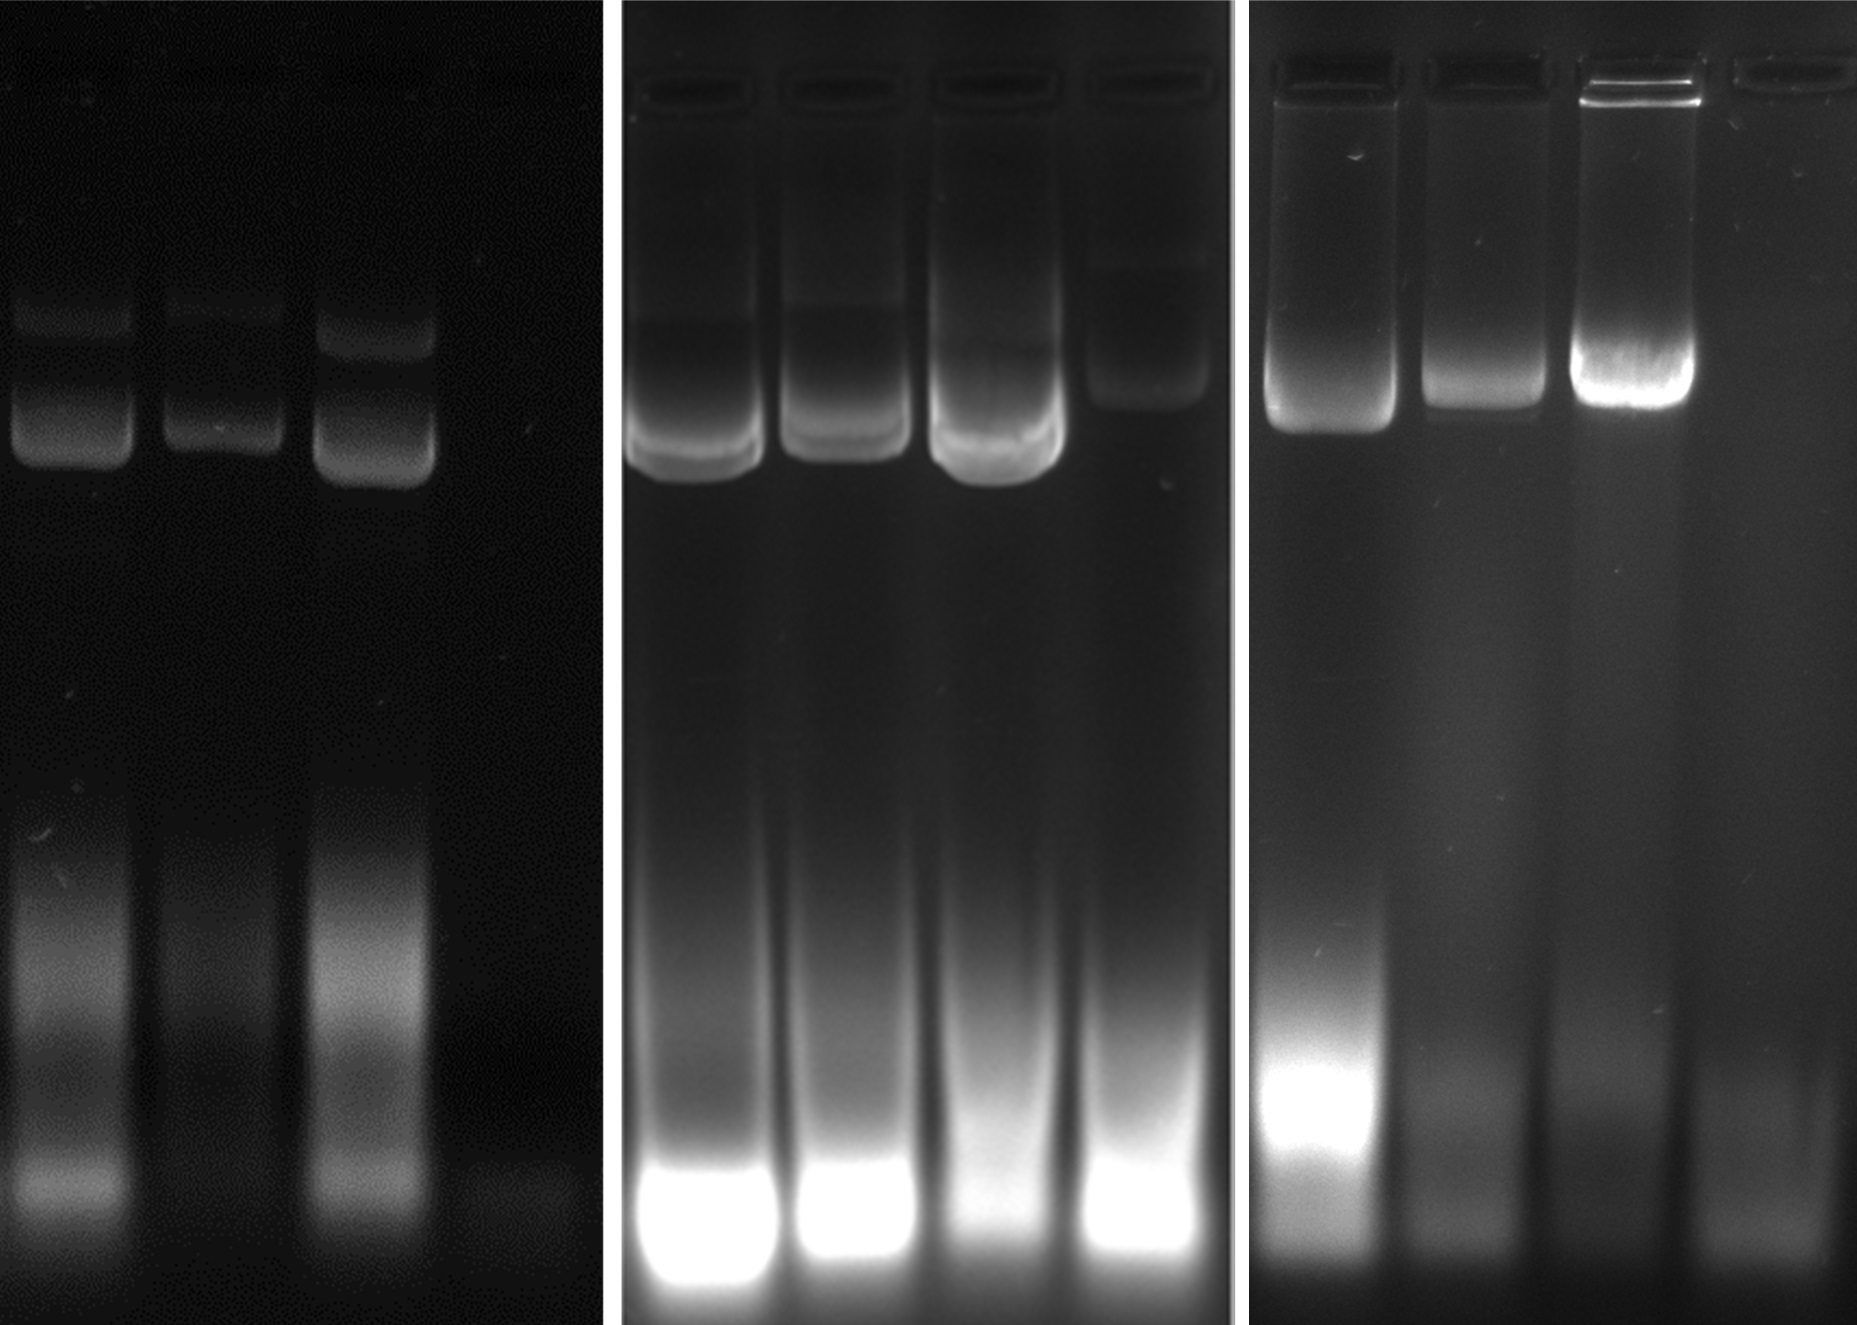
\includegraphics[width=8cm]{EFart4}};

\begin{scope}[font=\scriptsize]
\node[above] at (-3.65cm,2.85cm) {1};
\node[above] at (-3.025cm,2.85cm) {2};
\node[above] at (-2.4cm,2.85cm) {3};
\node[above] at (-1.775cm,2.85cm) {4};

\node[above] at (-1cm,2.85cm) {5};
\node[above] at (-0.375cm,2.85cm) {6};
\node[above] at (0.275cm,2.85cm) {7};
\node[above] at (0.975cm,2.85cm) {8};

\node[above] at (1.75cm,2.85cm) {9};
\node[above] at (2.39cm,2.85cm) {10};
\node[above] at (3.05cm,2.85cm) {11};
\node[above] at (3.725cm,2.85cm) {12};

\draw (4.1,1.35) -- (4.25,1.35) -- (4.35,1.6) -- (4.5,1.6)  node[right,align=left] {\pCAMBIA\\(9--12)};
\draw (4.1,1) -- (4.5,1) node[right,align=left] {\pVAX\\(1--8)};
%\draw (2.6,0.9) -- (3,0.9) node[right] {pDNA (sc)};
\draw (4.1,-1.8) -- (4.5,-1.8) node[right] {HMw\,RNA};
\draw (4.1,-2.5) -- (4.5,-2.5) node[right] {LMw\,RNA};

\end{scope}

\end{tikzpicture}
	\caption[Análise por eletroforese em gel de agarose dos ensaios de ultrafiltração.]{Análise por AGE dos seguintes ensaios: (1--4) MF do lisado da fermentação \pVAX\ seguida de UF a 3.7\,\micro m/s e $\agitacao=760$\,min$^{-1}$, com a membrana \emph{FS40PP} (1-lisado, 2-MFP, 3-UFC, 4-UFC). (5--8) MF do lisado da fermentação do \pVAX\ seguida de UF a 2.4\,\micro m/s e $\agitacao=760$\,min$^{-1}$ com a membrana \emph{Biomax 300} (5-lisado, 6-MFP, 7-UFC, 8-UFP). (9--12) MF do lisado da fermentação com \pCAMBIA\ seguido de UF a 2.4\,\micro m/s e $\agitacao=760$\,min$^{-1}$ com a membrana \emph{Biomax 300} (9-lisado, 10-MFP, 11-UFC, 12-UFP).}
	\label{fig:6art4}
\end{figure}
% subsection 3.2art4 (end)

\subsection{Resultados isolamento intermediário} % (fold)
\label{sub:iso_interm_at4}
\index{isolamento intermediário}%
Os resultados obtidos para os vários processos de isolamento intermediário de pDNA encontram-se na tabela~\ref{tab:res_isol_art4}. Para as condições operatórias escolhidas na realização dos vários ensaios verifica-se uma reduzida colmatação das membranas, colmatação essa representada pelo rácio entre a permeabilidade hidráulica das membranas no fim dos ensaios e as suas permeabilidades iniciais ($L_{\mr{p,f}}/L_{\mr{p},0}$).
\index{permeabilidade hidráulica}%
Este fator pode ter especial importância do ponto de vista de aplicação prática, uma vez que pode proporcionar um aumento no número de ciclos de utilização entre lavagens (ou substituição) de membranas, sendo este parâmetro um dos principais fatores de impacto ambiental e económico deste tipo de processos \cite{freitas}.
\begin{table}[!b]
\centering
	\caption[Resultados obtidos nos processos de isolamento intermediário.]{Resultados obtidos nos vários processos de isolamento intermediário estudados. Os valores encontram-se representados em percentagem com a indicação do respetivo desvio padrão obtido.}
	\label{tab:res_isol_art4}
	\begin{threeparttable}
\begin{tabular*}{0.75\textwidth}{l@{\extracolsep{\fill}} z{2} z{1} z{1} z{3}}
 \toprule
Processo & 
\mc{1}{l}{$L_{\mr{p,f}}/L_{\mr{p},0}$} &
\mc{1}{l}{$R_{\mr{pDNA}}$\tnote{a}} &
\mc{1}{l}{$R_{\mr{RNA}}$\tnote{b}} &
\mc{1}{l}{Pureza\tnote{c}} \\
\midrule
``A'' & 97.3 ? 1.7 & 98.6 ? 3.1 & 19.2 ? 6.1 &  9.53 ? 0.3 \\
``B'' & 87.2 ? 1.6 & 82.1 ? 2.8 & 96.5 ? 1.3 & 63.34 ? 6.1 \\
``C'' & 86.1 ? 1.0 & 95.7 ? 5.0 & 96.6 ? 1.1 & 38.99 ? 2.5 \\
``D'' &            & 88.6 ? 8.0 & 88.0 ? 1.9 & 35.74 ? 2.1 \\
\bottomrule
\end{tabular*}
\begin{tablenotes}
\item[a] Rendimento de recuperação de pDNA  
\item[b] Rendimento de remoção de RNA
\item[c] Pureza cromatográfica nas análises de HIC
\end{tablenotes}
\end{threeparttable}
\end{table}

Com a utilização da membrana com o poro de menores dimensões (FS40PP, Processo A), obtiveram-se elevados rendimentos de recuperação de pDNA, sendo este o processo que apresentou melhor performance neste domínio (tabela~\ref{tab:res_isol_art4}). No entanto, o rendimento de remoção de RNA obtido foi modesto, estando de acordo com os resultados obtidos no capítulo~\ref{chap:art3}. Contudo, é importante referir que este processo pode ainda assim ser útil no contexto do isolamento intermediário de pDNA, por exemplo em operações de concentração e de troca de tampão, dado os valores elevados de rendimento de recuperação de pDNA obtidos e o reduzido grau de colmatação das membranas verificado nestes ensaios.

Tal como referido anteriormente, para obter rendimentos de remoção de RNA mais elevados é necessário utilizar uma membrana com um poro de maiores dimensões. Assim, foi utilizada uma membrana de 300\,kDa de ``cut-off'' (Biomax\,300, $\raioporo = 25$\,nm). Procurou-se melhorar o valor de remoção de RNA através da utilização de uma operação de diafiltração (Processo B). Tal como se pode verificar na tabela~\ref{tab:res_isol_art4}, por este método obtém-se uma elevada remoção de RNA (cerca de 96.5\%), inclusivamente superior à que se obtém com o processo alternativo estudado (88\%, Processo D).
\index{RNA!rendimento de remoção}%
Contudo, o aumento do tamanho do poro conduz igualmente a uma diminuição do rendimento de recuperação de pDNA, por comparação com o Processo A, que se situou em 82\% neste processo. Este valor encontra-se ainda acima do limite mínimo de rendimento que se considera aceitável para uma operação unitária num processo de produção de pDNA \cite{kepka,smrekar,urthaler2}.
\index{DNA plasmídico!rendimento de recuperação}%
A perda de rendimento verificada deve-se essencialmente à permeação de parte do plasmídeo \pVAX\ na membrana, uma vez que grande parte do pDNA restante foi analisado no permeado (cerca de 14\%, em média, do plasmídeo presente inicialmente). A ocorrência de alguma permeação de pDNA, e concomitante elevada permeação das diferentes espécies de RNA presentes, está explicita na análise por eletroforese em gel de agarose de amostras recolhidas ao longo do processo (figura~\ref{fig:ef_processoB_art4}).
\index{AGE}% 
\begin{figure}[!t]
	\centering
	\begin{tikzpicture}

\node at (3cm, 3cm) {%\includegraphics[width=7cm]{% mudar para 6.3 cm
\includegraphics[width=6cm]{ef_processoB_art4.jpg}};

\fill[white] (-0.2cm, 0cm) rectangle (0.8cm, 5.5cm);
\fill[white] (5cm, 0cm) rectangle (6.1cm, 5.5cm);

\node[above, color = white] at (1.225, 4.9) {1};
\node[above, color = white] at (1.7, 4.9) {2};
\node[above, color = white] at (2.2, 4.9) {3};
\node[above, color = white] at (2.675, 4.9) {4};
\node[above, color = white] at (3.2, 4.9) {5};
\node[above, color = white] at (3.675, 4.9) {6};
\node[above, color = white] at (4.2, 4.9) {7};
\node[above, color = white] at (4.675, 4.9) {8};

\draw (5.1, 3.85) -- (5.5, 3.85) node[right] {pDNA\,(sc)};
\draw (5.1, 4.1) -- (5.25, 4.1) -- (5.35, 4.3) -- (5.5, 4.3) node[right] {pDNA\,(oc)}; 
\draw (5.1, 2.4) -- (5.5, 2.4) node[right] {HMw\,RNA};
\draw (5.1, 1.75) -- (5.5, 1.75) node[right] {LMw\,RNA}; 

% \draw[help lines] (0cm, 0cm) grid (8cm, 6cm);
\useasboundingbox (0cm, 0cm) rectangle (8cm, 6cm);

\end{tikzpicture}
	\caption[Análise de amostras, ao longo do processo B, por eletroforese em gel de agarose.]{Análise de amostras, ao longo do processo B, por eletroforese em gel de agarose. Estão representados os resultados obtidos em duas repetições do processo. Amostras 1 e 5: lisado; Amostras 2 e 6: permeado da microfiltração; Amostras 3 e 7; produto final obtido após diafiltração; Amostras 4 e 8: permeado conjunto da operação de ultrafiltração/diafiltração. Na figura é possível verificar a elevada permeação das várias espécies de RNA bem como alguma permeação do plasmídeo \pVAX.}
	\label{fig:ef_processoB_art4}
\end{figure}
Pode ainda ser acrescentado que este processo permitiu obter um valor de pureza cromatográfica bastante superior, quando comparado com o processo alternativo (Processo D), tal como pode ser observado na tabela~\ref{tab:res_isol_art4} e na figura~\ref{fig:hic_comparacao_art4}.
\index{pureza cromatográfica}%
A pureza cromatográfica foi calculada pelo rácio entre a área do pico referente ao plasmídeo e a área total do cromatograma, nas análises pelo método HIC. Na figura~\ref{fig:hic_comparacao_art4} encontram-se as análises de HIC do produto final dos dois processos. O cromatograma referente ao processo B apresenta uma notória superior remoção de contaminantes e consequentemente um valor mais elevado de pureza cromatográfica.
\begin{figure}[!t]
	\centering
	\begin{tikzpicture}

\begin{axis}[%
% xlabel style = {fill = white},
% x tick label style = {fill = white},
width=5cm,
height=6cm,
scale only axis,
% axis y line* = left,
% xmin=-5,
% xmax=85,
xlabel={$V_{\mr{R}}$\,[mL]},
% ymin=-500,
% ymax = 2,
ylabel={Absorvância 260\,nm [mAU]},
at={(0cm, 0cm)},
anchor=south west,
% ylabel near ticks
% legend style={at={(1.03,0.5)},legend columns=1,anchor=west,font=\scriptsize,draw=black,fill=white,legend cell align=left}
]
\addplot[
color=black,
solid
]
table[row sep=crcr]{
0.00000	0.00000\\
0.01000	-0.00319\\
0.02000	-0.00279\\
0.03000	-0.00003\\
0.04000	0.00800\\
0.05000	0.00800\\
0.06000	0.00684\\
0.07000	0.00310\\
0.08000	-0.00503\\
0.09000	-0.01060\\
0.10000	-0.01900\\
0.11000	-0.02172\\
0.12000	-0.02711\\
0.13000	-0.02996\\
0.14000	-0.02740\\
0.15000	-0.01600\\
0.16000	-0.01046\\
0.17000	-0.00101\\
0.18000	0.00385\\
0.19000	0.00287\\
0.20000	0.00900\\
0.21000	0.00102\\
0.22000	0.00243\\
0.23000	0.00360\\
0.24000	0.00708\\
0.25000	0.02400\\
0.26000	0.02072\\
0.27000	0.01969\\
0.28000	0.02318\\
0.29000	0.00789\\
0.30000	0.00888\\
0.31000	0.01552\\
0.32000	0.02325\\
0.33000	0.02541\\
0.34000	0.02423\\
0.35000	0.02292\\
0.36000	0.01889\\
0.37000	0.02303\\
0.38000	0.02763\\
0.39000	0.03353\\
0.40000	0.04330\\
0.41000	0.04494\\
0.42000	0.05299\\
0.43000	0.06001\\
0.44000	0.06100\\
0.45000	0.07314\\
0.46000	0.06984\\
0.47000	0.06196\\
0.48000	0.04930\\
0.49000	0.04746\\
0.50000	0.05140\\
0.51000	0.04581\\
0.52000	0.05822\\
0.53000	0.06233\\
0.54000	0.06167\\
0.55000	0.05450\\
0.56000	0.06139\\
0.57000	0.07566\\
0.58000	0.16256\\
0.59000	0.42631\\
0.60000	1.95446\\
0.61000	8.12856\\
0.62000	25.52763\\
0.63000	69.94649\\
0.64000	140.89924\\
0.65000	269.04561\\
0.66000	414.48015\\
0.67000	545.02997\\
0.68000	653.48344\\
0.69000	705.01673\\
0.70000	696.19861\\
0.71000	651.55936\\
0.72000	590.63611\\
0.73000	520.45869\\
0.74000	445.54502\\
0.75000	386.85822\\
0.76000	331.88873\\
0.77000	290.72830\\
0.78000	256.61163\\
0.79000	226.66150\\
0.80000	205.06388\\
0.81000	183.64954\\
0.82000	167.05330\\
0.83000	153.25521\\
0.84000	141.45760\\
0.85000	133.64444\\
0.86000	127.20937\\
0.87000	123.10997\\
0.88000	120.37367\\
0.89000	118.77187\\
0.90000	118.60709\\
0.91000	118.55548\\
0.92000	117.93753\\
0.93000	116.66145\\
0.94000	114.02649\\
0.95000	109.66127\\
0.96000	104.94424\\
0.97000	99.30794\\
0.98000	93.90067\\
0.99000	87.60856\\
1.00000	81.38730\\
1.01000	75.64406\\
1.02000	69.47163\\
1.03000	64.50407\\
1.04000	60.02512\\
1.05000	56.28509\\
1.06000	53.85458\\
1.07000	51.06158\\
1.08000	47.86160\\
1.09000	44.97569\\
1.10000	41.20834\\
1.11000	37.65127\\
1.12000	34.71720\\
1.13000	32.10887\\
1.14000	29.68245\\
1.15000	27.56398\\
1.16000	25.40531\\
1.17000	23.81828\\
1.18000	23.06117\\
1.19000	22.18864\\
1.20000	22.64264\\
1.21000	22.55848\\
1.22000	22.76408\\
1.23000	23.40284\\
1.24000	23.57731\\
1.25000	23.54345\\
1.26000	23.59975\\
1.27000	23.14316\\
1.28000	22.12947\\
1.29000	21.10960\\
1.30000	20.05726\\
1.31000	18.81123\\
1.32000	17.78075\\
1.33000	16.69056\\
1.34000	15.74811\\
1.35000	15.00334\\
1.36000	14.33357\\
1.37000	13.91543\\
1.38000	13.54449\\
1.39000	13.28825\\
1.40000	13.01713\\
1.41000	12.63920\\
1.42000	12.30297\\
1.43000	11.93290\\
1.44000	11.59175\\
1.45000	11.34565\\
1.46000	11.08482\\
1.47000	10.82204\\
1.48000	10.59200\\
1.49000	10.34684\\
1.50000	10.13829\\
1.51000	10.07100\\
1.52000	10.13183\\
1.53000	10.34814\\
1.54000	10.82641\\
1.55000	11.40114\\
1.56000	12.00786\\
1.57000	12.61584\\
1.58000	13.02598\\
1.59000	13.20546\\
1.60000	13.12087\\
1.61000	12.83750\\
1.62000	12.32358\\
1.63000	11.73703\\
1.64000	11.00704\\
1.65000	10.29940\\
1.66000	9.69510\\
1.67000	9.13187\\
1.68000	8.66831\\
1.69000	8.30152\\
1.70000	7.89327\\
1.71000	7.49074\\
1.72000	7.07692\\
1.73000	6.65769\\
1.74000	6.29790\\
1.75000	5.94366\\
1.76000	5.60424\\
1.77000	5.29557\\
1.78000	5.00575\\
1.79000	4.79466\\
1.80000	4.63104\\
1.81000	4.56859\\
1.82000	4.53370\\
1.83000	4.52477\\
1.84000	4.55740\\
1.85000	4.58895\\
1.86000	4.65239\\
1.87000	4.72644\\
1.88000	4.79895\\
1.89000	4.84448\\
1.90000	4.87022\\
1.91000	4.87427\\
1.92000	4.86187\\
1.93000	4.83097\\
1.94000	4.82099\\
1.95000	4.80904\\
1.96000	4.78674\\
1.97000	4.76374\\
1.98000	4.71430\\
1.99000	4.65011\\
2.00000	4.57981\\
2.01000	4.50510\\
2.02000	4.45320\\
2.03000	4.39894\\
2.04000	4.34534\\
2.05000	4.27717\\
2.06000	4.20933\\
2.07000	4.11948\\
2.08000	4.05992\\
2.09000	4.00561\\
2.10000	3.95988\\
2.11000	3.92508\\
2.12000	3.87424\\
2.13000	3.83032\\
2.14000	3.77495\\
2.15000	3.72877\\
2.16000	3.68692\\
2.17000	3.64255\\
2.18000	3.60118\\
2.19000	3.56594\\
2.20000	3.50460\\
2.21000	3.45769\\
2.22000	3.41567\\
2.23000	3.38039\\
2.24000	3.34236\\
2.25000	3.32477\\
2.26000	3.28807\\
2.27000	3.24316\\
2.28000	3.20442\\
2.29000	3.16406\\
2.30000	3.14202\\
2.31000	3.12577\\
2.32000	3.10121\\
2.33000	3.07144\\
2.34000	3.04011\\
2.35000	2.98315\\
2.36000	2.93968\\
2.37000	2.89214\\
2.38000	2.85858\\
2.39000	2.82993\\
2.40000	2.79946\\
2.41000	2.77372\\
2.42000	2.73963\\
2.43000	2.69805\\
2.44000	2.68058\\
2.45000	2.65845\\
2.46000	2.63724\\
2.47000	2.62007\\
2.48000	2.58733\\
2.49000	2.55330\\
2.50000	2.51948\\
2.51000	2.48068\\
2.52000	2.46078\\
2.53000	2.44331\\
2.54000	2.42252\\
2.55000	2.40547\\
2.56000	2.38328\\
2.57000	2.36654\\
2.58000	2.36145\\
2.59000	2.33838\\
2.60000	2.34639\\
2.61000	2.31576\\
2.62000	2.29207\\
2.63000	2.28277\\
2.64000	2.29608\\
2.65000	2.46760\\
2.66000	2.76167\\
2.67000	3.16447\\
2.68000	3.55412\\
2.69000	3.89542\\
2.70000	4.07660\\
2.71000	4.16248\\
2.72000	4.20010\\
2.73000	4.19282\\
2.74000	4.16519\\
2.75000	4.12419\\
2.76000	4.07371\\
2.77000	4.01668\\
2.78000	3.95456\\
2.79000	3.89149\\
2.80000	3.82833\\
2.81000	3.75442\\
2.82000	3.68804\\
2.83000	3.62076\\
2.84000	3.54983\\
2.85000	3.47941\\
2.86000	3.41364\\
2.87000	3.34973\\
2.88000	3.28613\\
2.89000	3.22421\\
2.90000	3.16082\\
2.91000	3.10042\\
2.92000	3.02966\\
2.93000	2.94451\\
2.94000	2.86216\\
2.95000	2.77067\\
2.96000	2.69081\\
2.97000	2.59595\\
2.98000	2.51150\\
2.99000	2.43694\\
3.00000	2.35344\\
3.01000	2.28912\\
3.02000	2.22104\\
3.03000	2.17172\\
3.04000	2.13077\\
3.05000	2.10550\\
3.06000	2.09381\\
3.07000	2.07932\\
3.08000	2.06688\\
3.09000	2.04627\\
3.10000	2.03125\\
3.11000	2.00600\\
3.12000	2.00251\\
3.13000	1.98645\\
3.14000	1.98271\\
3.15000	2.00273\\
3.16000	2.03123\\
3.17000	2.10707\\
3.18000	2.21989\\
3.19000	2.32294\\
3.20000	2.41643\\
3.21000	2.47721\\
3.22000	2.48459\\
3.23000	2.46117\\
3.24000	2.40479\\
3.25000	2.35822\\
3.26000	2.30255\\
3.27000	2.24843\\
3.28000	2.19948\\
3.29000	2.13964\\
3.30000	2.09073\\
3.31000	2.05307\\
3.32000	2.00626\\
3.33000	1.97273\\
3.34000	1.93367\\
3.35000	1.90875\\
3.36000	1.89557\\
3.37000	1.89337\\
3.38000	1.90407\\
3.39000	1.91539\\
3.40000	1.92419\\
3.41000	1.91021\\
3.42000	1.89760\\
3.43000	1.87660\\
3.44000	1.85253\\
3.45000	1.82824\\
3.46000	1.80228\\
3.47000	1.79405\\
3.48000	1.78278\\
3.49000	1.77345\\
3.50000	1.77057\\
3.51000	1.76248\\
3.52000	1.76096\\
3.53000	1.76517\\
3.54000	1.77464\\
3.55000	1.79440\\
3.56000	1.81054\\
3.57000	1.82904\\
3.58000	1.84705\\
3.59000	1.86491\\
3.60000	1.89725\\
3.61000	1.93743\\
3.62000	1.96374\\
3.63000	2.00504\\
3.64000	2.04833\\
3.65000	2.08834\\
3.66000	2.13421\\
3.67000	2.18709\\
3.68000	2.23058\\
3.69000	2.26622\\
3.70000	2.32402\\
3.71000	2.39094\\
3.72000	2.45459\\
3.73000	2.51906\\
3.74000	2.58221\\
3.75000	2.64627\\
3.76000	2.72471\\
3.77000	2.79790\\
3.78000	2.89682\\
3.79000	2.97547\\
3.80000	3.07014\\
3.81000	3.18751\\
3.82000	3.29545\\
3.83000	3.43502\\
3.84000	3.53800\\
3.85000	3.68840\\
3.86000	3.82627\\
3.87000	3.91215\\
3.88000	4.05097\\
3.89000	4.05901\\
3.90000	4.15232\\
3.91000	4.17164\\
3.92000	4.16251\\
3.93000	4.24416\\
3.94000	4.23491\\
3.95000	4.28271\\
3.96000	4.32541\\
3.97000	4.43170\\
3.98000	4.59979\\
3.99000	4.79163\\
4.00000	5.04350\\
4.01000	5.29676\\
4.02000	5.69280\\
4.03000	6.16688\\
4.04000	6.75612\\
4.05000	7.50441\\
4.06000	8.15056\\
4.07000	8.97493\\
4.08000	9.70150\\
4.09000	10.42212\\
4.10000	11.16584\\
4.11000	11.79421\\
4.12000	12.64509\\
4.13000	13.40227\\
4.14000	14.25354\\
4.15000	15.19466\\
4.16000	15.73232\\
4.17000	16.48164\\
4.18000	17.09590\\
4.19000	17.80193\\
4.20000	18.62849\\
4.21000	19.53557\\
4.22000	20.22566\\
4.23000	20.90787\\
4.24000	21.52656\\
4.25000	22.12303\\
4.26000	22.55921\\
4.27000	23.26982\\
4.28000	24.47958\\
4.29000	25.91480\\
4.30000	27.63320\\
4.31000	29.96465\\
4.32000	32.06548\\
4.33000	34.74787\\
4.34000	37.63365\\
4.35000	41.10140\\
4.36000	45.19253\\
4.37000	49.54535\\
4.38000	54.85259\\
4.39000	60.53994\\
4.40000	66.16454\\
4.41000	72.15323\\
4.42000	77.71702\\
4.43000	82.70860\\
4.44000	87.46207\\
4.45000	91.00652\\
4.46000	94.40213\\
4.47000	97.11617\\
4.48000	99.16921\\
4.49000	101.06455\\
4.50000	102.32452\\
4.51000	103.01482\\
4.52000	103.21476\\
4.53000	102.88253\\
4.54000	102.01101\\
4.55000	100.71815\\
4.56000	98.76823\\
4.57000	96.48269\\
4.58000	93.93680\\
4.59000	90.92388\\
4.60000	87.60919\\
4.61000	84.53308\\
4.62000	81.02874\\
4.63000	77.76603\\
4.64000	74.57315\\
4.65000	71.27362\\
4.66000	68.35089\\
4.67000	65.04720\\
4.68000	61.96309\\
4.69000	58.85874\\
4.70000	55.63381\\
4.71000	52.91539\\
4.72000	50.07222\\
4.73000	47.55988\\
4.74000	45.15644\\
4.75000	42.76165\\
4.76000	40.67474\\
4.77000	38.41351\\
4.78000	36.25217\\
4.79000	34.35585\\
4.80000	32.38986\\
4.81000	30.56755\\
4.82000	28.95376\\
4.83000	27.18077\\
4.84000	25.68802\\
4.85000	24.08466\\
4.86000	22.55590\\
4.87000	21.16442\\
4.88000	19.65941\\
4.89000	18.42333\\
4.90000	17.04910\\
4.91000	15.78362\\
4.92000	14.62056\\
4.93000	13.32487\\
4.94000	12.28534\\
4.95000	11.19995\\
4.96000	10.26399\\
4.97000	9.42838\\
4.98000	8.51727\\
4.99000	7.64440\\
5.00000	6.83945\\
5.01000	5.99580\\
5.02000	5.25097\\
5.03000	4.56911\\
5.04000	3.88284\\
5.05000	3.37127\\
5.06000	2.81764\\
5.07000	2.33053\\
5.08000	1.90527\\
5.09000	1.46590\\
5.10000	1.10800\\
5.11000	0.73184\\
5.12000	0.41717\\
5.13000	0.12073\\
5.14000	-0.19100\\
5.15000	-0.42836\\
5.16000	-0.62051\\
5.17000	-0.78765\\
5.18000	-0.90242\\
5.19000	-1.01362\\
5.20000	-1.19228\\
5.21000	-1.35079\\
5.22000	-1.51336\\
5.23000	-1.61413\\
5.24000	-1.68453\\
5.25000	-1.72327\\
5.26000	-1.73603\\
5.27000	-1.79946\\
5.28000	-1.84925\\
5.29000	-1.89296\\
5.30000	-1.96796\\
5.31000	-2.00622\\
5.32000	-2.03996\\
5.33000	-2.03148\\
5.34000	-2.00886\\
5.35000	-1.99070\\
5.36000	-1.96980\\
5.37000	-1.97376\\
5.38000	-1.96482\\
5.39000	-1.91655\\
5.40000	-1.86026\\
5.41000	-1.83430\\
5.42000	-1.81350\\
5.43000	-1.79188\\
5.44000	-1.73618\\
5.45000	-1.66766\\
5.46000	-1.57019\\
5.47000	-1.50275\\
5.48000	-1.47324\\
5.49000	-1.44965\\
5.50000	-1.42930\\
5.51000	-1.38329\\
5.52000	-1.32752\\
5.53000	-1.27476\\
5.54000	-1.20521\\
5.55000	-1.18050\\
5.56000	-1.16695\\
5.57000	-1.15809\\
5.58000	-1.14435\\
5.59000	-1.13400\\
5.60000	-1.10244\\
5.61000	-1.05576\\
5.62000	-1.03224\\
5.63000	-1.01775\\
5.64000	-0.99700\\
5.65000	-0.96975\\
5.66000	-0.91049\\
5.67000	-0.84752\\
5.68000	-0.79440\\
5.69000	-0.75800\\
5.70000	-0.76238\\
5.71000	-0.75126\\
5.72000	-0.72543\\
5.73000	-0.69923\\
5.74000	-0.65100\\
5.75000	-0.60880\\
5.76000	-0.57952\\
5.77000	-0.54787\\
5.78000	-0.51701\\
5.79000	-0.49300\\
5.80000	-0.47882\\
5.81000	-0.45840\\
5.82000	-0.45457\\
5.83000	-0.44244\\
5.84000	-0.44000\\
5.85000	-0.43919\\
5.86000	-0.43654\\
5.87000	-0.43391\\
5.88000	-0.41182\\
5.89000	-0.37800\\
5.90000	-0.35461\\
5.91000	-0.34370\\
5.92000	-0.33697\\
5.93000	-0.32753\\
5.94000	-0.30600\\
5.95000	-0.27737\\
5.96000	-0.24307\\
5.97000	-0.22623\\
5.98000	-0.23295\\
5.99000	-0.23000\\
6.00000	-0.22717\\
6.01000	-0.21657\\
6.02000	-0.19682\\
6.03000	-0.17877\\
6.04000	-0.16800\\
6.05000	-0.16894\\
6.06000	-0.18215\\
6.07000	-0.19958\\
6.08000	-0.20630\\
6.09000	-0.20300\\
6.10000	-0.18260\\
6.11000	-0.18400\\
6.12000	-0.19313\\
6.13000	-0.19449\\
6.14000	-0.20064\\
6.15000	-0.17438\\
6.16000	-0.15101\\
6.17000	-0.12780\\
6.18000	-0.11683\\
6.19000	-0.10279\\
6.20000	-0.10326\\
6.21000	-0.09238\\
6.22000	-0.08544\\
6.23000	-0.07824\\
6.24000	-0.06232\\
6.25000	-0.04904\\
6.26000	-0.04355\\
6.27000	-0.04388\\
6.28000	-0.03561\\
6.29000	-0.03424\\
6.30000	-0.03977\\
6.31000	-0.03841\\
6.32000	-0.03407\\
6.33000	-0.02986\\
6.34000	-0.02215\\
6.35000	-0.01415\\
6.36000	-0.00641\\
6.37000	-0.00300\\
6.38000	0.01363\\
6.39000	0.01291\\
6.40000	0.00884\\
6.41000	0.01673\\
6.42000	0.02427\\
6.43000	0.05134\\
6.44000	0.07217\\
6.45000	0.08820\\
6.46000	0.10174\\
6.47000	0.10590\\
6.48000	0.10337\\
6.49000	0.10653\\
6.50000	0.11497\\
};
\end{axis}

\begin{axis}[%
% xlabel style = {fill = white},
% x tick label style = {fill = white},
width=5cm,
height=6cm,
scale only axis,
% axis y line* = left,
% xmin=-5,
% xmax=85,
xlabel={$V_{\mr{R}}$\,[mL]},
% ymin=-500,
% ymax = 2,
ylabel={Absorvância 260\,nm [mAU]},
at={(7cm, 0cm)},
anchor=south west,
% ylabel near ticks
% legend style={at={(1.03,0.5)},legend columns=1,anchor=west,font=\scriptsize,draw=black,fill=white,legend cell align=left}
]
\addplot[
color=black,
solid
]
table[row sep=crcr]{
0.00000	-0.00700\\
0.01000	-0.00873\\
0.02000	-0.00696\\
0.03000	0.00249\\
0.04000	0.00929\\
0.05000	0.00400\\
0.06000	0.01167\\
0.07000	0.00462\\
0.08000	-0.00200\\
0.09000	0.00623\\
0.10000	0.00600\\
0.11000	0.00688\\
0.12000	0.01850\\
0.13000	0.02346\\
0.14000	0.02917\\
0.15000	0.03652\\
0.16000	0.03316\\
0.17000	0.03672\\
0.18000	0.03286\\
0.19000	0.02163\\
0.20000	0.02159\\
0.21000	0.00955\\
0.22000	-0.00012\\
0.23000	0.00239\\
0.24000	0.00028\\
0.25000	-0.00100\\
0.26000	0.00034\\
0.27000	-0.00034\\
0.28000	-0.00755\\
0.29000	-0.00617\\
0.30000	-0.00941\\
0.31000	-0.00985\\
0.32000	-0.01210\\
0.33000	-0.01904\\
0.34000	-0.02774\\
0.35000	-0.03103\\
0.36000	-0.03075\\
0.37000	-0.03481\\
0.38000	-0.04208\\
0.39000	-0.04545\\
0.40000	-0.05116\\
0.41000	-0.04763\\
0.42000	-0.03947\\
0.43000	-0.02384\\
0.44000	-0.01466\\
0.45000	-0.01007\\
0.46000	-0.00439\\
0.47000	-0.00706\\
0.48000	-0.00957\\
0.49000	-0.00497\\
0.50000	-0.01141\\
0.51000	-0.01290\\
0.52000	-0.01648\\
0.53000	-0.00861\\
0.54000	-0.01500\\
0.55000	-0.01069\\
0.56000	0.01159\\
0.57000	0.04894\\
0.58000	0.18378\\
0.59000	0.61100\\
0.60000	2.37909\\
0.61000	9.04055\\
0.62000	23.79902\\
0.63000	53.99250\\
0.64000	109.90791\\
0.65000	191.20209\\
0.66000	310.68517\\
0.67000	434.74980\\
0.68000	557.19306\\
0.69000	661.51227\\
0.70000	714.78269\\
0.71000	725.42193\\
0.72000	703.26391\\
0.73000	662.68690\\
0.74000	605.87336\\
0.75000	544.09205\\
0.76000	488.54387\\
0.77000	429.63476\\
0.78000	381.72000\\
0.79000	336.33798\\
0.80000	298.30458\\
0.81000	268.65373\\
0.82000	241.11600\\
0.83000	221.49314\\
0.84000	205.29036\\
0.85000	193.36954\\
0.86000	185.03668\\
0.87000	178.98529\\
0.88000	173.55717\\
0.89000	169.16855\\
0.90000	163.53787\\
0.91000	157.07783\\
0.92000	149.48168\\
0.93000	140.10797\\
0.94000	130.88085\\
0.95000	119.99089\\
0.96000	109.89251\\
0.97000	100.27925\\
0.98000	90.65280\\
0.99000	82.15819\\
1.00000	75.45313\\
1.01000	68.66970\\
1.02000	63.24337\\
1.03000	58.25521\\
1.04000	53.91932\\
1.05000	51.21372\\
1.06000	49.54607\\
1.07000	50.17788\\
1.08000	51.96600\\
1.09000	53.19993\\
1.10000	53.89093\\
1.11000	52.85703\\
1.12000	51.17828\\
1.13000	49.48499\\
1.14000	48.54685\\
1.15000	47.68732\\
1.16000	46.52343\\
1.17000	45.59597\\
1.18000	43.50301\\
1.19000	41.13944\\
1.20000	38.35003\\
1.21000	34.73732\\
1.22000	30.87917\\
1.23000	26.95239\\
1.24000	22.89586\\
1.25000	19.43877\\
1.26000	16.98642\\
1.27000	15.23673\\
1.28000	14.54185\\
1.29000	14.63769\\
1.30000	15.14816\\
1.31000	15.99996\\
1.32000	17.08131\\
1.33000	18.29304\\
1.34000	19.43757\\
1.35000	20.71154\\
1.36000	21.84233\\
1.37000	22.95613\\
1.38000	24.04970\\
1.39000	24.98286\\
1.40000	25.93809\\
1.41000	26.75627\\
1.42000	27.55533\\
1.43000	28.37639\\
1.44000	29.04347\\
1.45000	29.72952\\
1.46000	30.38150\\
1.47000	30.89602\\
1.48000	31.42232\\
1.49000	31.91517\\
1.50000	32.39417\\
1.51000	32.91524\\
1.52000	33.37744\\
1.53000	33.86454\\
1.54000	34.33241\\
1.55000	34.73733\\
1.56000	35.19138\\
1.57000	35.63412\\
1.58000	36.08825\\
1.59000	36.58560\\
1.60000	37.07608\\
1.61000	37.54729\\
1.62000	37.96614\\
1.63000	38.27716\\
1.64000	38.56372\\
1.65000	38.74689\\
1.66000	38.84674\\
1.67000	38.88093\\
1.68000	38.76210\\
1.69000	38.63230\\
1.70000	38.50331\\
1.71000	38.46146\\
1.72000	38.50876\\
1.73000	38.55796\\
1.74000	38.63335\\
1.75000	38.65625\\
1.76000	38.66392\\
1.77000	38.64213\\
1.78000	38.62306\\
1.79000	38.59285\\
1.80000	38.48769\\
1.81000	38.38593\\
1.82000	38.23477\\
1.83000	38.04029\\
1.84000	37.85745\\
1.85000	37.63212\\
1.86000	37.43348\\
1.87000	37.21157\\
1.88000	36.98005\\
1.89000	36.76116\\
1.90000	36.49099\\
1.91000	36.21447\\
1.92000	35.97308\\
1.93000	35.71618\\
1.94000	35.47871\\
1.95000	35.25406\\
1.96000	35.01343\\
1.97000	34.77192\\
1.98000	34.52682\\
1.99000	34.29234\\
2.00000	34.08456\\
2.01000	33.85465\\
2.02000	33.66683\\
2.03000	33.46071\\
2.04000	33.26932\\
2.05000	33.08376\\
2.06000	32.89445\\
2.07000	32.71238\\
2.08000	32.56530\\
2.09000	32.39812\\
2.10000	32.26091\\
2.11000	32.10962\\
2.12000	31.95310\\
2.13000	31.82501\\
2.14000	31.69523\\
2.15000	31.57314\\
2.16000	31.44848\\
2.17000	31.30061\\
2.18000	31.14801\\
2.19000	30.98297\\
2.20000	30.82907\\
2.21000	30.68543\\
2.22000	30.53624\\
2.23000	30.39348\\
2.24000	30.25421\\
2.25000	30.09197\\
2.26000	29.93939\\
2.27000	29.77061\\
2.28000	29.60055\\
2.29000	29.44049\\
2.30000	29.26424\\
2.31000	29.11737\\
2.32000	28.93883\\
2.33000	28.75687\\
2.34000	28.58157\\
2.35000	28.38499\\
2.36000	28.19349\\
2.37000	28.03223\\
2.38000	27.85891\\
2.39000	27.68437\\
2.40000	27.50665\\
2.41000	27.31034\\
2.42000	27.17603\\
2.43000	27.02971\\
2.44000	26.88779\\
2.45000	26.73531\\
2.46000	26.53632\\
2.47000	26.33820\\
2.48000	26.13457\\
2.49000	25.96612\\
2.50000	25.81186\\
2.51000	25.66062\\
2.52000	25.50830\\
2.53000	25.37518\\
2.54000	25.22284\\
2.55000	25.08915\\
2.56000	24.94206\\
2.57000	24.80359\\
2.58000	24.68608\\
2.59000	24.50758\\
2.60000	24.18710\\
2.61000	24.02617\\
2.62000	23.88819\\
2.63000	23.90431\\
2.64000	23.94248\\
2.65000	23.95212\\
2.66000	23.98716\\
2.67000	23.96563\\
2.68000	23.89051\\
2.69000	23.81380\\
2.70000	23.73125\\
2.71000	23.67109\\
2.72000	23.58316\\
2.73000	23.49352\\
2.74000	23.41064\\
2.75000	23.31608\\
2.76000	23.22385\\
2.77000	23.13115\\
2.78000	23.03910\\
2.79000	22.94109\\
2.80000	22.83477\\
2.81000	22.75401\\
2.82000	22.65840\\
2.83000	22.55806\\
2.84000	22.47357\\
2.85000	22.38612\\
2.86000	22.28051\\
2.87000	22.20385\\
2.88000	22.11816\\
2.89000	22.03431\\
2.90000	21.95894\\
2.91000	21.86538\\
2.92000	21.78862\\
2.93000	21.69123\\
2.94000	21.59524\\
2.95000	21.51637\\
2.96000	21.42424\\
2.97000	21.32698\\
2.98000	21.25488\\
2.99000	21.16374\\
3.00000	21.08190\\
3.01000	21.00295\\
3.02000	20.92259\\
3.03000	20.84505\\
3.04000	20.75575\\
3.05000	20.68133\\
3.06000	20.60456\\
3.07000	20.53649\\
3.08000	20.47584\\
3.09000	20.40237\\
3.10000	20.33381\\
3.11000	20.24973\\
3.12000	20.17478\\
3.13000	20.11493\\
3.14000	20.07042\\
3.15000	20.04232\\
3.16000	20.02933\\
3.17000	20.03527\\
3.18000	20.03961\\
3.19000	20.04087\\
3.20000	20.03434\\
3.21000	19.99745\\
3.22000	19.93673\\
3.23000	19.86937\\
3.24000	19.79278\\
3.25000	19.70305\\
3.26000	19.62397\\
3.27000	19.55150\\
3.28000	19.46868\\
3.29000	19.40609\\
3.30000	19.34804\\
3.31000	19.29786\\
3.32000	19.25014\\
3.33000	19.21594\\
3.34000	19.19278\\
3.35000	19.15146\\
3.36000	19.11590\\
3.37000	19.08538\\
3.38000	19.04128\\
3.39000	19.00517\\
3.40000	18.98909\\
3.41000	18.97566\\
3.42000	18.96090\\
3.43000	18.93642\\
3.44000	18.91207\\
3.45000	18.87689\\
3.46000	18.84804\\
3.47000	18.85576\\
3.48000	18.87555\\
3.49000	18.89495\\
3.50000	18.90094\\
3.51000	18.89914\\
3.52000	18.88795\\
3.53000	18.90447\\
3.54000	18.94409\\
3.55000	19.00082\\
3.56000	19.04669\\
3.57000	19.09810\\
3.58000	19.14383\\
3.59000	19.19350\\
3.60000	19.25399\\
3.61000	19.34318\\
3.62000	19.44659\\
3.63000	19.52530\\
3.64000	19.61056\\
3.65000	19.67234\\
3.66000	19.73446\\
3.67000	19.82380\\
3.68000	19.92650\\
3.69000	20.05886\\
3.70000	20.17607\\
3.71000	20.27151\\
3.72000	20.35377\\
3.73000	20.42427\\
3.74000	20.50422\\
3.75000	20.63997\\
3.76000	20.80452\\
3.77000	20.94201\\
3.78000	21.09778\\
3.79000	21.25924\\
3.80000	21.40727\\
3.81000	21.62958\\
3.82000	21.96328\\
3.83000	22.31927\\
3.84000	22.72152\\
3.85000	23.11950\\
3.86000	23.54309\\
3.87000	24.02296\\
3.88000	24.62838\\
3.89000	25.37197\\
3.90000	26.22904\\
3.91000	27.09149\\
3.92000	28.15276\\
3.93000	29.25434\\
3.94000	30.47172\\
3.95000	31.82892\\
3.96000	33.45338\\
3.97000	35.07096\\
3.98000	36.73567\\
3.99000	38.66475\\
4.00000	40.54294\\
4.01000	42.73235\\
4.02000	44.94819\\
4.03000	47.39942\\
4.04000	50.18954\\
4.05000	53.06643\\
4.06000	55.84341\\
4.07000	59.23410\\
4.08000	62.27136\\
4.09000	65.59845\\
4.10000	69.47663\\
4.11000	73.16937\\
4.12000	77.51315\\
4.13000	81.63307\\
4.14000	86.17131\\
4.15000	90.74788\\
4.16000	94.93919\\
4.17000	99.91953\\
4.18000	104.37699\\
4.19000	109.07752\\
4.20000	114.11587\\
4.21000	119.15242\\
4.22000	123.80138\\
4.23000	129.01897\\
4.24000	133.68775\\
4.25000	138.86605\\
4.26000	143.98252\\
4.27000	149.05765\\
4.28000	154.73117\\
4.29000	159.63099\\
4.30000	164.94128\\
4.31000	169.91934\\
4.32000	174.45100\\
4.33000	179.16929\\
4.34000	183.63879\\
4.35000	187.25421\\
4.36000	190.91620\\
4.37000	193.92867\\
4.38000	196.52000\\
4.39000	198.70077\\
4.40000	200.04678\\
4.41000	200.97321\\
4.42000	201.23761\\
4.43000	200.91325\\
4.44000	200.05795\\
4.45000	198.69666\\
4.46000	196.62887\\
4.47000	194.25093\\
4.48000	191.38174\\
4.49000	187.87485\\
4.50000	184.06016\\
4.51000	180.28692\\
4.52000	175.81392\\
4.53000	171.66409\\
4.54000	166.96346\\
4.55000	162.05178\\
4.56000	157.42614\\
4.57000	152.07017\\
4.58000	147.28748\\
4.59000	142.11653\\
4.60000	136.98950\\
4.61000	132.20278\\
4.62000	126.87865\\
4.63000	122.24146\\
4.64000	117.22820\\
4.65000	112.23982\\
4.66000	107.60946\\
4.67000	103.28352\\
4.68000	98.68131\\
4.69000	94.79262\\
4.70000	90.57300\\
4.71000	86.64068\\
4.72000	82.94498\\
4.73000	79.09599\\
4.74000	75.85762\\
4.75000	72.31188\\
4.76000	69.10729\\
4.77000	66.07347\\
4.78000	62.81722\\
4.79000	60.06689\\
4.80000	57.10655\\
4.81000	54.23765\\
4.82000	51.67270\\
4.83000	49.10372\\
4.84000	46.56443\\
4.85000	44.33006\\
4.86000	41.86000\\
4.87000	39.75711\\
4.88000	37.64298\\
4.89000	35.52000\\
4.90000	33.72399\\
4.91000	31.79347\\
4.92000	30.09289\\
4.93000	28.37552\\
4.94000	26.73451\\
4.95000	25.22916\\
4.96000	23.86270\\
4.97000	22.42963\\
4.98000	21.27181\\
4.99000	20.01282\\
5.00000	18.87533\\
5.01000	17.87073\\
5.02000	16.81677\\
5.03000	15.91793\\
5.04000	15.01270\\
5.05000	14.21975\\
5.06000	13.48557\\
5.07000	12.71228\\
5.08000	12.11916\\
5.09000	11.48640\\
5.10000	10.88026\\
5.11000	10.38660\\
5.12000	9.92603\\
5.13000	9.44078\\
5.14000	9.06747\\
5.15000	8.68306\\
5.16000	8.35673\\
5.17000	8.02566\\
5.18000	7.71422\\
5.19000	7.47831\\
5.20000	7.20469\\
5.21000	7.00104\\
5.22000	6.81486\\
5.23000	6.62285\\
5.24000	6.45645\\
5.25000	6.27732\\
5.26000	6.12100\\
5.27000	5.99896\\
5.28000	5.86926\\
5.29000	5.76667\\
5.30000	5.67286\\
5.31000	5.55574\\
5.32000	5.47420\\
5.33000	5.38690\\
5.34000	5.30361\\
5.35000	5.25016\\
5.36000	5.18854\\
5.37000	5.13174\\
5.38000	5.05100\\
5.39000	4.96839\\
5.40000	4.90847\\
5.41000	4.83707\\
5.42000	4.78177\\
5.43000	4.72900\\
5.44000	4.66362\\
5.45000	4.60051\\
5.46000	4.53128\\
5.47000	4.46878\\
5.48000	4.41000\\
5.49000	4.33544\\
5.50000	4.28123\\
5.51000	4.22145\\
5.52000	4.15676\\
5.53000	4.10400\\
5.54000	4.04689\\
5.55000	3.98161\\
5.56000	3.91954\\
5.57000	3.85587\\
5.58000	3.78527\\
5.59000	3.73395\\
5.60000	3.67270\\
5.61000	3.62595\\
5.62000	3.58254\\
5.63000	3.53996\\
5.64000	3.49990\\
5.65000	3.45784\\
5.66000	3.41139\\
5.67000	3.35692\\
5.68000	3.30011\\
5.69000	3.25892\\
5.70000	3.21425\\
5.71000	3.16105\\
5.72000	3.11156\\
5.73000	3.07992\\
5.74000	3.03382\\
5.75000	3.00080\\
5.76000	2.96592\\
5.77000	2.92950\\
5.78000	2.87927\\
5.79000	2.84251\\
5.80000	2.80575\\
5.81000	2.76402\\
5.82000	2.73223\\
5.83000	2.70362\\
5.84000	2.68211\\
5.85000	2.65223\\
5.86000	2.62131\\
5.87000	2.58700\\
5.88000	2.56138\\
5.89000	2.53458\\
5.90000	2.51492\\
5.91000	2.49457\\
5.92000	2.46400\\
5.93000	2.44414\\
5.94000	2.41541\\
5.95000	2.39317\\
5.96000	2.37325\\
5.97000	2.36100\\
5.98000	2.33742\\
5.99000	2.30812\\
6.00000	2.28523\\
6.01000	2.26068\\
6.02000	2.23500\\
6.03000	2.21775\\
6.04000	2.20998\\
6.05000	2.19948\\
6.06000	2.18717\\
6.07000	2.17360\\
6.08000	2.16489\\
6.09000	2.14412\\
6.10000	2.13059\\
6.11000	2.12314\\
6.12000	2.11425\\
6.13000	2.09757\\
6.14000	2.08893\\
6.15000	2.07800\\
6.16000	2.07447\\
6.17000	2.06556\\
6.18000	2.05335\\
6.19000	2.03819\\
6.20000	2.02414\\
6.21000	2.01151\\
6.22000	1.99499\\
6.23000	1.98558\\
6.24000	1.97833\\
6.25000	1.96666\\
6.26000	1.95092\\
6.27000	1.93508\\
6.28000	1.90853\\
6.29000	1.90277\\
6.30000	1.90118\\
6.31000	1.90255\\
6.32000	1.89880\\
6.33000	1.88879\\
6.34000	1.86421\\
6.35000	1.85817\\
6.36000	1.85156\\
6.37000	1.83271\\
6.38000	1.83209\\
6.39000	1.82421\\
6.40000	1.81243\\
6.41000	1.80494\\
6.42000	1.80737\\
6.43000	1.80847\\
6.44000	1.80890\\
6.45000	1.81340\\
6.46000	1.80731\\
6.47000	1.80178\\
6.48000	1.79344\\
6.49000	1.78308\\
6.50000	1.78296\\
};
\end{axis}

% \draw[help lines] (-2cm, -2cm) grid (14cm, 8cm);

\node[right] at (0, 6.5) {Processo B (produto final)};
\node[right] at (7, 6.5) {Processo D (produto final)};

\node[below left, font = \scriptsize] at (5, 6) {HIC};
\node[below left, font = \scriptsize] at (12, 6) {HIC};

\end{tikzpicture}
	\caption[Cromatogramas HIC do produto final dos processos B e C.]{Perfil cromatográfico, obtido com o método de HIC, dos produtos finais referentes aos processos B e D. Na figura é notório o aumento do valor da pureza cromatográfica obtida com o processo à base de operações de membranas (processo B).}
	\label{fig:hic_comparacao_art4}
\end{figure}

O modelo desenvolvido prevê uma menor permeação do plasmídeo \pCAMBIA\ nas condições operatórias utilizadas nos processos de isolamento primário, nomeadamente um fluxo de 2.4\,\micro m/s e uma velocidade de agitação de 760\,\minmum\ (ver figura~\ref{fig:1dart4}). Deste modo, foi assim testado o processo de isolamento intermediário na purificação deste plasmídeo (processo C, figura~\ref{fig:processos_art4}). Como se pode observar na tabela~\ref{tab:res_isol_art4}, obteve-se um elevado rendimento de recuperação de pDNA (95.7\%), acompanhado de um igualmente elevado rendimento de remoção de RNA (96.7\%), indicando assim uma satisfatória seletividade do processo para efetuar a separação pDNA/RNA, facto nunca antes obtido recorrendo unicamente a processos de membranas \cite{kahn,duvaltff,freitas}. O menor valor obtido para este processo, em termos da pureza cromatográfica, fica-se a dever à menor concentração do plasmídeo \pCAMBIA\ nos lisados (tabela~\ref{tab:1art4}).
\index{pCAMBIA@\pCAMBIA}%
% section 3art4 (end)

\section{Conclusões} % (fold)
\label{sec:4art4}
A separação entre o pDNA e as várias espécies de RNA pode ser obtida por ultrafiltração. Para isso é fundamental otimizar quer o tamanho do poro da membrana quer o valor do fluxo de filtração. O desenvolvimento de um modelo teórico com capacidade de prever as permeações observadas de pDNA e RNA revelou-se decisivo na escolha dos parâmetros operacionais. Este modelo, originalmente desenvolvido para sistemas de 3 componentes (o plasmídeo, um contra-ião e um co-ião), com o objetivo de contabilizar o efeito da força iónica da solução nos valores de permeação de pDNA, foi neste capítulo estendido para um sistema de 4 componentes (o plasmídeo, uma espécie de RNA, um contra-ião e um co-ião). Os efeitos mútuos da permeação simultânea de pDNA e RNA foram investigados, com os resultados a mostrarem que a permeação de RNA é fortemente afetada pela presença das moléculas de pDNA, causando uma redução dos seus valores de \permobs. Os resultados experimentais confirmam as previsões do modelo, nomeadamente ao comprovarem que a escolha de uma membrana com poro de 25\,nm, operada a baixos fluxos, é a melhor escolha para efetuar a referida separação. 

A separação pode ser ainda otimizada efetuando uma diafiltração após o passo de concentração. Foram testados 3 processos de isolamento intermediário recorrendo a operações de separação com membranas. Os resultados obtidos confirmam as previsões do modelo, nomeadamente a reduzida permeação de pDNA na membrana com o poro de menores dimensões, acompanhada de uma igualmente reduzida permeação de RNA, em especial de HMw\,RNA. A utilização deste processo, apesar de revelar uma reduzida capacidade de remoção de RNA, apresenta valores bastante elevados de rendimento de recuperação de pDNA e valores mínimos de colmatação, características necessárias à obtenção de um processo com excelente capacidade de efetuar operações de concentração e de troca de tampão. A utilização de uma membrana com um poro de maiores dimensões, para as condições operatórias ótimas determinadas pelo modelo, permitiu obter elevados rendimentos de remoção dos vários tipos de RNA. Em especial, a aplicação do processo no isolamento intermediário do plasmídeo \pCAMBIA\ permitiu obter resultados, quer de recuperação de pDNA quer de remoção de RNA, que revelaram ser consideravelmente melhores quando comparados com os que se obtêm por intermédio de um processo alternativo usado em laboratório e que gera um maior impacto ambiental e económico, em especial de um ponto de vista de aplicação industrial. Para o caso do plasmídeo \pVAX, apesar de se obter novamente um elevado rendimento de remoção de RNA, o rendimento de recuperação de pDNA revelou ser mais reduzido, sendo que a perda de rendimento se deve essencialmente à maior permeação deste plasmídeo pela membrana. Com base no modelo teórico desenvolvido, prevê-se que possa vir a ser possível reduzir o valor de permeação, quer pelo aumento da concentração de \pVAX\ nos lisados quer pela redução da força iónica da solução, recorrendo por exemplo a uma operação prévia de concentração ou de dessalinização. Assim, criadas as condições para assegurar uma reduzida permeação de pDNA, a remoção de RNA poderá ser aumentada se no processo forem utilizados volumes de diafiltração mais elevados, sendo este um tema para trabalho futuro.
% section 4art4 (end)
%!TEX root = tese.tex
\chapter{Conclusão e perspetivas de trabalho futuro} % (fold)
\label{cha:conc}
No trabalho publicado em 2003 por Eon-Duval \et\ \cite{duvaltff}, no âmbito da utilização de uma operação de ultrafiltração no isolamento intermediário de DNA plasmídico, é possível ler o seguinte:
\begin{quote}
``\ldots As membranas de ultrafiltração utilizadas foram desenvolvidas para a purificação de proteínas e o seu ``cut-off'' determinado pela retenção de proteínas globulares. Contrariamente a proteínas globulares, o DNA plasmídico é uma molécula longa e fina, o que dificulta a previsão do seu comportamento em operações de ultrafiltração. Apesar do tamanho médio de plasmídeos para fins terapêuticos ser de vários milhões de Daltons, o tamanho de poro selecionado neste estudo para reter o plasmídeo é consideravelmente inferior \ldots'' 
\end{quote}
De facto, tal como afirmado por Eon-Duval \et, a permeação de plasmídeos em membranas de micro e ultrafiltração revela um comportamento completamente distinto do caso de proteínas globulares, que essencialmente se podem modelar como esferas rígidas e para as quais existem modelos bem estabelecidos na literatura. No caso do pDNA, é um facto bem conhecido que este exibe valores de permeação significativos em membranas com poros de tamanho consideravelmente inferiores. Este comportamento impede assim a aplicação dos modelos de esferas rígidas para prever a permeação de pDNA em membranas de micro e ultrafiltração. Na presente tese de doutoramento procurou-se superar esta limitação pelo desenvolvimento de novos modelos que possam contabilizar efeitos da deformação molecular induzida pelas tensões de corte geradas à entrada dos poros, e assim permitir explicar este fenómeno. O conceito de deformação molecular foi igualmente explorado por outros autores. No entanto, apesar de o trabalho desenvolvido ser de inquestionável valor e de ter proporcionado importantes avanços no estado do conhecimento nesta matéria, os modelos desenvolvidos apresentam algumas desvantagens que podem ser enumeradas, e que foram previamente discutidas na secção~\ref{sec:modulaçãopermeação}. 

Com a realização do presente trabalho foi possível obter uma ampliação do espectro de aplicação do modelo do transporte restringido, provavelmente o modelo mais citado e utilizado no âmbito das operações de micro e ultrafiltração. Com esta nova abordagem passa a ser possível aplicar o modelo, não só a moléculas com uma geometria rígida, como também a moléculas que exibem elevados graus de flexibilidade e como consequência valores significativos de permeação em poros com tamanhos inferiores. As moléculas foram modeladas como cadeias FJC e CSC e os seus coeficientes de partição determinados por simulações estocásticas. Nestas simulações determina-se a distribuição radial da probabilidade de uma molécula entrar no poro estabelecendo uma condição de entrada. No presente trabalho considerou-se como condição de entrada que a massa pontual mais perto do poro deverá estar projetada no interior do mesmo. Foi possível determinar uma equação que relaciona o coeficiente de partição com \lambdag, e verificou-se que a equação é válida tanto para a abordagem FJC, como para a abordagem CSC. 

A ligação com o modelo do transporte restringido foi feita notando que para moléculas longas e flexíveis, cujo tamanho é superior ao do poro, o fator de impedimento difusivo, dado pelo rácio entre o coeficiente de difusão das moléculas no interior do poro e o coeficiente de difusão numa situação não confinada, tende para zero. Por outro lado, o fator de impedimento convectivo deverá ser igual a 1, assumindo que estas moléculas uma vez no interior de poros com menores dimensões deverão mover-se com a velocidade média do solvente. Verifica-se, pois, que o coeficiente de permeação intrínseca se torna igual ao coeficiente de partição.

O desenvolvimento teórico proposto neste trabalho teve por base as equações de Maxwell-Stefan. Com esta abordagem, verifica-se que as principais equações usadas nos modelos podem ser deduzidas com base no mesmo princípio teórico. A polarização de concentração pode ser obtida com recurso ao modelo do filme. Nestas condições, e considerando soluções diluídas e ideais, foi possível deduzir e aplicar a equação de Nernst-Planck na camada de polarização de concentração. Esta equação revela-se fundamental para determinar a polarização de concentração do DNA plasmídico dado que este tipo de moléculas apresenta uma elevada carga elétrica. A equação de Nernst-Planck introduz importantes efeitos na permeação de moléculas com carga. Em especial, os vários compostos iónicos em solução exercem uma influência mútua entre si, influência esta que se manifesta pelo surgimento de um potencial elétrico na camada de polarização. Assim, para além do fluxo de filtração e dos coeficientes de difusão, a concentração e valência elétrica dos iões desempenham um papel importante no estabelecimento dos gradientes de concentração na camada de polarização e consequentemente nos valores da permeação observada dos vários componentes da solução a filtrar.

No decorrer do trabalho verificou-se que as moléculas de RNA também exibem permeação em poros com dimensões inferiores às dimensões moleculares. Este facto leva assim à necessidade de considerar igualmente efeitos de deformação molecular para explicar a sua permeação. Neste domínio, o facto do desenvolvimento do modelo para o pDNA ter sido efetuado de um modo mais abrangente possibilitou a sua aplicação ao caso do RNA, uma molécula que revela igualmente um enorme potencial como fármaco de segunda geração, e onde os processos de membranas deverão ter aplicabilidade na sua produção. O modelo aplicado ao RNA permitiu obter previsões em concordância com os resultados experimentais. A descrição da sua polarização de concentração revelou também a importância da utilização da equação de Nernst-Planck, uma vez que a permeação de RNA na presença de pDNA revelou ser quase independente do fluxo de filtração, o que só pode ser explicado por efeitos de carga. Por outro lado, o modelo desenvolvido prevê, para as concentrações das espécies estudadas neste trabalho, que a influência da presença de RNA na permeação de pDNA é muito menos significativa, facto que também foi verificado na prática.

É importante referir que a dedução da equação de Nernst-Planck mostra o elevado número de simplificações que é necessário efetuar. Em especial, têm que ser consideradas soluções diluídas e ideais para a equação ser aplicável. Por outro lado, o efeito da pressão no potencial químico tem que ser desprezado, o que para solutos com elevados volumes parciais molares pode não ser o melhor procedimento. Em processos de ultrafiltração, em especial em operações de concentração, a aproximação de soluções diluídas e ideais pode igualmente apresentar-se como uma descrição pouco realista. No entanto, não é menos verdade que a complexidade inerente a processos de micro e ultrafiltração, em especial a ocorrência de colmatação e subsequente alteração físico-química da membrana, não permite garantir que mesmo um modelo teórico mais preciso possa descrever com exatidão todo o fenómeno de permeação. A introdução de novos termos na equação de Nernst-Planck aumenta consideravelmente a dificuldade de integração dos sistemas de equações diferenciais. Esta dificuldade surge pelo facto dos valores que se procuram calcular (as concentrações dos vários componentes no permeado) precisarem de ser conhecidos para proceder à integração das equações de forma direta. Para superar esta limitação foi desenvolvido um algoritmo que permite, de forma iterativa, estimar estes valores e ir efetuando novas estimativas mais precisas até se obter uma aceitável convergência. Naturalmente, à medida que um maior número de componentes é considerado nos cálculos a complexidade inerente é aumentada significativamente, pelo que o desenvolvimento de algoritmos mais eficientes é assim premente. 

No presente trabalho foi determinado o coeficiente de partição de moléculas longas e flexíveis em dois passos: pela representação da estrutura das moléculas por modelos FJC e CSC e pela simulação estocástica necessária para determinar a probabilidade de entrada destas estruturas em poros. Foi considerada como condição necessária de entrada no poro que a massa pontual mais perto do poro esteja projetada no seu interior, sendo a restante molécula forçada a permear pelo efeito de deformação causado pelas tensões de corte geradas pelo fluxo convectivo do solvente. A utilização deste procedimento permitiu obter previsões com uma satisfatória aproximação aos resultados experimentais. No entanto, verificou-se uma certa tendência para subestimar ligeiramente as permeações. Neste domínio, poderão obviamente ser efetuados alguns melhoramentos, como por exemplo na determinação experimental de condições de entrada em poros que possam descrever de forma mais realista o fenómeno de permeação. As representações FJC e CSC são igualmente representações que poderão ser demasiado simples para descrever a estrutura de pDNA e RNA. Por exemplo, nestas representações não é tido em conta o efeito do volume excluído, que pode desempenhar um papel importante. Estes dois efeitos poderão contribuir para que se verifiquem previsões de permeação geralmente mais elevadas do que as que se observam na prática. No entanto, do mesmo modo poderá ser referido que o incremento da complexidade na análise do problema gera incontornavelmente um enorme aumento no esforço, quer computacional quer de realização de ensaios experimentais, sem que exista uma clara certeza que a exatidão das previsões seja significativamente melhorada, o que se deve, tal como referido anteriormente, à elevada complexidade inerente aos processos de micro e ultrafiltração.

Os modelos teóricos desenvolvidos para estimar a permeação de pDNA consideram apenas a sua isoforma super-enrolada. Este facto deve-se em parte à escassez de dados na literatura que permitam estimar de forma precisa as propriedades das várias isoformas. Como trabalho futuro seria importante procurar alargar o modelo para permitir a sua aplicação diferenciada às várias isoformas de pDNA, que inevitavelmente são parte integrante dos lisados. Variações nos valores de permeação para diferentes isoformas, em processos de ultrafiltração, foi já verificada na prática \cite{zydneyiso} e a obtenção de um modelo teórico com capacidade de previsão constituiria uma ferramenta de inegável valor neste domínio, em especial tendo em consideração a importância da separação de isoformas num processo de produção de pDNA.

De um ponto de vista de aplicação prática foi possível obter uma elevada seletividade na sepração pDNA/RNA por ultrafiltração. Neste aspeto, os modelos desenvolvidos revelaram-se essenciais para estimar as condições operatórias necessárias. O modelo previu a utilização de membranas com poros de razoáveis dimensões (20--25\,nm) operadas a fluxos de filtração reduzidos. A utilização de baixos fluxos gera a possibilidade de reter o pDNA permitindo uma elevada permeação das moléculas de RNA. Por outro lado, devido aos reduzidos valores do coeficiente de difusão das moléculas de pDNA, fluxos baixos permitem obter uma menor polarização de concentração e consequente inferior grau de colmatação. Este facto pode gerar um aumento no tempo dos ciclos de utilização entre lavagens e uma redução na periodicidade de substituição de membranas. Por outro lado, minimizam a adsorção de compostos, facto que conduz a indesejadas alterações físico-químicas das membranas, o que pode levar a uma redução da reprodutibilidade entre filtrações. Este modo de operação a fluxo constante e de reduzido valor não é o mais utilizado, por exemplo em esquemas de purificação de proteínas. Para a sua implementação poderá ser necessário desenhar novos módulos de filtração que permitam efetuar um controlo preciso do fluxo de filtração. Por outro lado, fluxos reduzidos implicam a necessidade de utilizar uma maior área de membrana para obter uma produtividade semelhante. Assim, a viabilidade do processo terá que ser necessariamente avaliada tendo em conta as inerentes vantagens e desvantagens do método. No entanto, o processo de ultrafiltração/diafiltração desenvolvido no presente trabalho permite a eliminação da utilização de elevadas quantidades de agentes precipitantes, o que naturalmente tem o potencial de gerar um menor impacto ambiental e económico.   

No âmbito da produção e purificação de DNA plasmídico é essencial obter métodos de quantificação que permitam, de forma célere e eficiente, quantificar não só o plasmídeo como também os vários contaminantes ao longo do processo. Nesta matéria, o método cromatográfico de HIC, desenvolvido por Diogo \et\ \cite{diogo}, revela possuir ótimas características para tal, nomeadamente uma boa reprodutibilidade, robustez, ausência de pré-tratamento das amostras (com exceção da remoção do conteúdo sólido) e rapidez de execução. No presente trabalho de doutoramento sugere-se que o RNA possa ser igualmente analisado por este método, permitindo uma análise simultânea conjuntamente com o pDNA. Para controlo de qualidade da preparação final de pDNA deverá ser preciso efetuar uma análise mais precisa do conteúdo de RNA, no entanto, para controlar os rendimentos de remoção desta biomolécula em fases intermédias do processo de produção verifica-se que o método de HIC pode constituir uma excelente alternativa.

Na presente tese de doutoramento procurou-se estudar a remoção de sólidos, originados pelo processo de lise alcalina, recorrendo ao uso de uma operação de microfiltração. Outras processos alternativos podem ser considerados, como por exemplo centrifugação, filtração convencional e flutuação forçada. No entanto, a centrifugação é geralmente considerada como pouco viável à escala industrial. Filtração convencional e operações de flutuação forçada não permitem garantir a total remoção de conteúdo sólido, pelo menos de uma forma tão segura como a que se obtém com uma operação de microfiltração. Este fator pode ter importância em especial para situações em que a operação subsequente apresente uma reduzida tolerância à presença de sólidos na corrente de entrada, como por exemplo operações de cromatografia. No presente trabalho foi estudada a microfiltração de um lisado alcalino. Foram obtidos elevados rendimentos de recuperação de pDNA e completa remoção de sólidos aquando da utilização de uma membrana hidrofílica de Nylon com um poro nominal de 0.2\,\micro m, a um fluxo de filtração constante de 73\,L/h$\cdot$m$^2$. Durante a filtração dos lisados foi, contudo, observada alguma re-dissolução de gDNA durante o processo. Verificou-se que este efeito não poderia ser explicado apenas pela redução da força iónica do lisado durante o processo, e que teria de ser, portanto, resultante da degradação mecânica do conteúdo precipitado pela ação das tensões de corte geradas. De facto, observou-se que o gDNA re-dissolvido apresentou valores de permeação significativos numa membrana de ultrafiltração com um poro de tamanho reduzido ($\raioporo = 4$\,nm), confirmando a ideia de que a ação mecânica imposta no material precipitado leva a re-dissolução de pequenos fragmentos de gDNA, que como é sabido podem causar complicações em fases mais avançadas do processo. Este resultado está assim de acordo com a ideia de ser necessário impor, durante operações de separação sólido-líquido a seguir à lise, reduzidas tensões de corte para evitar a re-dissolução de contaminantes. Apesar disso, também se verificou que na segunda operação de membranas, a ultrafiltração, é possível remover de forma eficientemente estes fragmentos contaminantes.    

Nos ensaios de microfiltração, referidos no parágrafo anterior, observou-se a ocorrência de alguma colmatação das membranas. Devido à elevada quantidade de sólidos e de contaminantes dissolvidos nos lisados este fenómeno será sempre, em maior ou menor grau, uma inevitabilidade. Uma forma de procurar rentabilizar a operação e de reduzir o impacto ambiental e económico subjacente passa por desenvolver novas membranas que possam ser produzidas de forma económica e que sejam biodegradáveis. Nos nosso laboratórios estão a ser dados passos nesta direção como comprova um estudo recentemente publicado \cite{meues}.  


\cleardoublepage
\phantomsection
\addcontentsline{toc}{chapter}{Bibliografia}
\bibliographystyle{elsart-num}
\bibliography{bibliografia}

\appendix

%!TEX root=tese.tex
\chapter{Determinação da concentração mássica de células para efetuar a lise}
\label{app:1}
Para determinar a concentração mássica de células (peso húmido) a usar na etapa de lise foram realizados ensaios prévios de estabilidade de lisados. Para isso, efetuou-se a lise alcalina de suspensões de células com diferentes concentrações mássicas (figura~\ref{fig:estabilidade_lisados}). A concentração mássica foi determinada como o rácio entre o peso húmido de células e o volume de tampão usado na sua ressuspensão. Os lisados obtidos foram posteriormente processados por centrifugação para remover o conteúdo sólido formado durante a lise. Como se pode verificar na figura~\ref{fig:estabilidade_lisados}, para as concentrações de 180 e 240 g/L, observa-se um aumento da densidade ótica dos lisados centrifugados ao longo do tempo, facto que indica a ocorrência da precipitação de algum do material inicialmente dissolvido. Optou-se por escolher a concentração de 120\,g/L, para a qual se verificou um reduzido aumento da densidade ótica, estando este valor igualmente dentro da gama de concentrações usadas por outros autores \cite{theo,chamsart,urthaler}. Com a escolha deste valor de concentração pretende-se assim evitar a ocorrência da precipitação de alguns constituintes do lisado em operações subsequentes à etapa da lise alcalina, facto que poderia introduzir efeitos indesejados na interpretação e desempenho dos processos.
\index{concentração!mássica de células}
\index{peso húmido}
\index{lisado!estabilidade} 
\begin{figure}[!h]
    \centering
    \begin{tikzpicture}

\begin{axis}[
	width=6cm,
	height=6cm,
	scale only axis,
	xmin=0,
	xmax=25,
	xlabel={$t_{\mr{inc}}$\,[h]},
	ymin=0,
	ymax=0.06,
	ylabel={OD 600\,nm},
	ylabel near ticks,
	at={(0cm,0cm)},
	anchor=south west,
	legend style={at={(1.03,0.5)},legend columns=1,anchor=west,font=\scriptsize,draw=black,fill=white,legend cell align=left}
	]
\addplot[
color=black,
solid,
mark=*,
mark options={solid,fill=black,draw=black}
]
table[row sep=crcr]{
0.000000 0.001500\\
1.000000 0.001000\\
2.000000 0.001500\\
3.000000 0.002500\\
4.000000 0.002000\\
6.333333 0.001500\\
24.00000 0.000000\\
};\addlegendentry{60\,g/L};

\addplot[
color=black,
dashed,
mark=*,
mark options={solid,fill=white,draw=black}
]
table[row sep=crcr]{
0.000000 0.000500\\
1.000000 0.003000\\
2.000000 0.003000\\
3.000000 0.003500\\
4.000000 0.003500\\
6.333333 0.003500\\
24.00000 0.002000\\
};\addlegendentry{120\,g/L};

\addplot[
color=black,
dashdotted,
mark=triangle*,
mark options={solid,fill=black,draw=black}
]
table[row sep=crcr]{
0.000000 0.002000\\
1.000000 0.004500\\
2.000000 0.006000\\
3.000000 0.008000\\
4.000000 0.011500\\
6.333333 0.010500\\
24.00000 0.004500\\
};\addlegendentry{180\,g/L};

\addplot[
color=black,
dashdotdotted,
mark=triangle,
mark options={solid,fill=white,draw=black}
]
table[row sep=crcr]{
0.000000 0.007000\\
1.000000 0.019500\\
2.000000 0.021500\\
3.000000 0.032000\\
4.000000 0.040500\\
6.333333 0.045500\\
24.00000 0.048000\\
};\addlegendentry{240\,g/L};

\end{axis}

\end{tikzpicture}
    \caption[Densidade ótica de lisados em função do tempo de incubação]{Variação da densidade ótica (600\,nm) em função do tempo de incubação para lisados alcalinos centrifugados a diferentes valores de concentração mássica de células (peso húmido).}
    \label{fig:estabilidade_lisados}
\end{figure}

\chapter{Caracterização de lisados centrifugados}
\label{app:2}
Foram utilizados dois géis de SEC diferentes: o gel Sephacryl S-1000 SF e o gel Sephacryl S-100 HR (\emph{GE Healthcare}), estando as suas principais características indicadas na tabela~\ref{tab:sephacryl}.\index{Sephacryl S-1000!características}\index{Sephacryl S-100!características} 
\begin{table}
\caption[Principais características dos géis Sephacryl S-100 HR e Spehacryl S-1000 SF]{Principais características dos géis Sephacryl S-100 HR e Spehacryl S-1000 SF \cite{sec}.}
\label{tab:sephacryl}
\begin{tabularx}{\textwidth}{Y Y Y Y Y} 
 \toprule
Gel & Intervalo de fracionamento [kDa] & Capacidade & Caudal recomendado & Tamanho médio das partículas \\
 \midrule  
Sephacryl \newline S-100 HR & 1--100 & 0.4\%--4\% do volume total de coluna & 10--35\,cm/h & 47\,\micro m \\
Sphacryl \newline S-1000 SF & $500-5\times 10^{5}$ & 0.4\%--4\% do volume total de coluna & 2--30\,cm/h & 65\,\micro m \\
\bottomrule 
\end{tabularx}
\end{table}

Para efetuar a análise de lisados por SEC, os géis foram empacotados numa coluna com 50\,mL de volume (\emph{Sigma}), segundo as recomendações do fabricante. Obteve-se no final um volume de gel de aproximadamente 46\,mL. A coluna foi conectada a um sistema cromatográfico (Äkta purifier, \emph{GE Healthcare}) e as amostras de lisado foram injetadas e eluídas a um caudal de 0.5\,mL/min, usando tampão Tris/HCl 10\,mM a pH 8.00, com 150\,mM de NaCl, como eluente. A absorvância do eluato foi continuamente monitorizada a 260\,nm. Em alguns ensaios foram recolhidas amostras do eluído em intervalos de 10\,min. Estas amostras foram posteriormente analisadas por AGE, HIC e BCA.\index{coluna cromatográfica}\index{AGE}\index{BCA}\index{akta@Äkta}

Na figura~\ref{fig:s1000} encontra-se o resultado da análise do lisado de \pVAX\ no gel Sephacryl S-1000 SF. No cromatograma obtido (figura~\ref{fig:s1000}~a) é possível identificar dois picos parcialmente sobrepostos. No primeiro pico elui o plasmídeo, que essencialmente é recolhido nas frações 4 e 5 (figura~\ref{fig:s1000}~c). Devido à existência no lisado de várias espécies de RNA, estas biomoléculas eluem ao longo do segundo pico, com a prevista tendência da redução de tamanhos ao longo das várias frações. Nas análises de HIC das frações selecionadas (figura~\ref{fig:s1000}~b), verifica-se a presença de plasmídeo apenas na fração 5. A área do pico na região 3 (contaminantes hidrofóbicos) diminui ao longo das frações, e na fração 10, que já parece não conter RNA, é nula. Na região 2 (contaminantes hidrofílicos), observa-se uma tendência contrária, registando-se uma maior absorvância na fração 9. Este facto parece indicar que os compostos que eluem na região 2 apresentam uma menor massa molecular.\index{cromatograma}\index{SEC!cromatograma}\index{lisado!SEC}\index{DNA plasmídico!SEC}\index{RNA!SEC}
\begin{figure}[!t]
    \centering
    \begin{tikzpicture}[scale = 0.9]
%\draw[help lines] (0cm, 0cm) grid (17cm, 14cm);

\node[font = \large, below] at (1.5, 14) {a)};
\node[font = \large, below] at (1.5, 8.5) {b)};
\node[font = \large, below] at (1.5, 2.5) {c)};

\draw (12.1, 1.2) -- (12.25, 1.2) -- (12.35, 1.6) -- (12.5, 1.6)  node[right] {pDNA\,(oc)};
\draw (12.1, 1) -- (12.5, 1) node[right] {pDNA\,(sc)};
\draw (12.1, -0.1) -- (12.5, -0.1) node[right] {HMw\,RNA};
\draw (12.1, -0.75) -- (12.5, -0.75) node[right] {LMw\,RNA};

\node[
below right,
align = right
] at (10.75, 13.75) {Sephacryl \\ S-1000 SF};

\node[below left, font = \scriptsize] at (4, 7) {HIC};
\node[below left, font = \scriptsize] at (8, 7) {HIC};
\node[below left, font = \scriptsize] at (12, 7) {HIC};
\node[below left, font = \scriptsize] at (16, 7) {HIC};

\draw[dashed] (4.7, 9) -- (4.7, 10);
\node[above, font = \scriptsize] at (4.95, 10) {1};
\draw[dashed] (5.2, 9) -- (5.2, 10);
\node[above, font = \scriptsize] at (5.45, 10) {2};
\draw[dashed] (5.699, 9) -- (5.699, 10);
\node[above, font = \scriptsize] at (5.95, 10) {3};
\draw[dashed] (6.199, 9) -- (6.199, 10);
\node[above, font = \scriptsize] at (6.45, 10) {4};
\draw[dashed] (6.699, 9) -- (6.699, 10);
\node[above, font = \scriptsize] at (6.95, 10) {5};
\draw[dashed] (7.199, 9) -- (7.199, 10);
\node[above, font = \scriptsize] at (7.45, 10) {6};
\draw[dashed] (7.699, 9) -- (7.699, 10);
\node[above, font = \scriptsize] at (7.95, 10) {7};
\draw[dashed] (8.199, 9) -- (8.199, 10);
\node[above, font = \scriptsize] at (8.45, 10) {8};
\draw[dashed] (8.699, 9) -- (8.699, 10);
\node[above, font = \scriptsize] at (8.95, 10) {9};
\draw[dashed] (9.199, 9) -- (9.199, 10);
\node[above, font = \scriptsize] at (9.45, 10) {10};
\draw[dashed] (9.699, 9) -- (9.699, 10);
\node[above, font = \scriptsize] at (9.95, 10) {11};
\draw[dashed] (10.199, 9) -- (10.199, 10);

\draw[dashed] (6.699, 9) -- (1, 7) (7.199, 9) -- (4, 7);
\draw[dashed] (7.699, 9) -- (5, 7) (8.199, 9) -- (8, 7);
\draw[dashed] (8.699, 9) -- (9, 7) (9.199, 9) -- (12, 7);
\draw[dashed] (9.199, 9) -- (13, 7) (9.699, 9) -- (16, 7);

\begin{axis}[%
xlabel style = {fill = white},
x tick label style = {fill = white},
width=9cm,
height=5cm,
scale only axis,
xmin=-5,
xmax=85,
xlabel={$V_{\mr{R}}$\,[mL]},
% ymin=-500,
% ymax=3000,
ylabel={Absorvância 260\,nm [AU]},
at={(4cm, 9cm)},
anchor=south west,
% legend style={at={(1.03,0.5)},legend columns=1,anchor=west,font=\scriptsize,draw=black,fill=white,legend cell align=left}
]
\addplot[
color=black,
solid
]
table[row sep=crcr]{
0.000000 0.000005\\
0.080000 -0.000012\\
0.160000 0.000005\\
0.240000 0.000059\\
0.320000 0.000017\\
0.400000 0.000023\\
0.480000 -0.000002\\
0.560000 0.000060\\
0.640000 0.000044\\
0.720000 0.000039\\
0.800000 0.000035\\
0.880000 0.000059\\
0.960000 0.000075\\
1.040000 0.000104\\
1.120000 0.000095\\
1.200000 0.000111\\
1.280000 0.000095\\
1.360000 0.000057\\
1.440000 0.000107\\
1.520000 0.000103\\
1.600000 0.000046\\
1.680000 0.000048\\
1.760000 0.000120\\
1.840000 0.000120\\
1.920000 0.000129\\
2.000000 0.000183\\
2.080000 0.000143\\
2.160000 0.000135\\
2.240000 0.000152\\
2.320000 0.000160\\
2.400000 0.000169\\
2.480000 0.000147\\
2.560000 0.000194\\
2.640000 0.000182\\
2.720000 0.000199\\
2.800000 0.000187\\
2.880000 0.000206\\
2.960000 0.000218\\
3.040000 0.000225\\
3.120000 0.000284\\
3.200000 0.000272\\
3.280000 0.000303\\
3.360000 0.000301\\
3.440000 0.000318\\
3.520000 0.000301\\
3.600000 0.000306\\
3.680000 0.000301\\
3.760000 0.000320\\
3.840000 0.000331\\
3.920000 0.000276\\
4.000000 0.000310\\
4.080000 0.000267\\
4.160000 0.000336\\
4.240000 0.000333\\
4.320000 0.000298\\
4.400000 0.000313\\
4.480000 0.000383\\
4.560000 0.000355\\
4.640000 0.000422\\
4.720000 0.000438\\
4.800000 0.000422\\
4.880000 0.000442\\
4.960000 0.000490\\
5.040000 0.000476\\
5.120000 0.000474\\
5.200000 0.000459\\
5.280000 0.000442\\
5.360000 0.000481\\
5.440000 0.000469\\
5.520000 0.000481\\
5.600000 0.000439\\
5.680000 0.000495\\
5.760000 0.000536\\
5.841000 0.000485\\
5.921000 0.000528\\
6.001000 0.000499\\
6.081000 0.000539\\
6.161000 0.000575\\
6.241000 0.000599\\
6.321000 0.000559\\
6.401000 0.000599\\
6.481000 0.000593\\
6.561000 0.000581\\
6.641000 0.000623\\
6.721000 0.000642\\
6.801000 0.000636\\
6.881000 0.000636\\
6.961000 0.000643\\
7.041000 0.000668\\
7.121000 0.000605\\
7.201000 0.000655\\
7.281000 0.000658\\
7.361000 0.000641\\
7.441000 0.000681\\
7.521000 0.000636\\
7.601000 0.000685\\
7.681000 0.000694\\
7.761000 0.000664\\
7.841000 0.000684\\
7.921000 0.000750\\
8.001000 0.000756\\
8.081000 0.000759\\
8.161000 0.000759\\
8.241000 0.000778\\
8.321000 0.000777\\
8.401000 0.000780\\
8.481000 0.000821\\
8.561000 0.000790\\
8.641000 0.000817\\
8.721000 0.000820\\
8.801000 0.000808\\
8.881000 0.000800\\
8.961000 0.000828\\
9.041000 0.000815\\
9.121000 0.000818\\
9.201000 0.000810\\
9.281000 0.000805\\
9.361000 0.000759\\
9.441000 0.000729\\
9.521000 0.000733\\
9.601000 0.000759\\
9.681000 0.000773\\
9.761000 0.000719\\
9.841000 0.000752\\
9.921000 0.000747\\
10.001000 0.000761\\
10.081000 0.000743\\
10.161000 0.000772\\
10.241000 0.000800\\
10.321000 0.000828\\
10.401000 0.000803\\
10.481000 0.000799\\
10.561000 0.000806\\
10.641000 0.000872\\
10.721000 0.000835\\
10.801000 0.000841\\
10.881000 0.000886\\
10.961000 0.000870\\
11.041000 0.000905\\
11.121000 0.000924\\
11.201000 0.000942\\
11.281000 0.000974\\
11.361000 0.000968\\
11.441000 0.000999\\
11.521000 0.001064\\
11.601000 0.001090\\
11.681000 0.001165\\
11.761000 0.001267\\
11.841000 0.001266\\
11.921000 0.001366\\
12.001000 0.001408\\
12.081000 0.001464\\
12.161000 0.001530\\
12.241000 0.001664\\
12.321000 0.001752\\
12.401000 0.001932\\
12.481000 0.001998\\
12.561000 0.002184\\
12.641000 0.002308\\
12.721000 0.002368\\
12.801000 0.002537\\
12.881000 0.002776\\
12.961000 0.002944\\
13.041000 0.003114\\
13.121000 0.003309\\
13.201000 0.003526\\
13.281000 0.003781\\
13.361000 0.003993\\
13.441000 0.004228\\
13.521000 0.004460\\
13.601000 0.004752\\
13.681000 0.005081\\
13.761000 0.005402\\
13.841000 0.005729\\
13.921000 0.006023\\
14.001000 0.006396\\
14.081000 0.006765\\
14.161000 0.007122\\
14.241000 0.007506\\
14.321000 0.007924\\
14.401000 0.008374\\
14.481000 0.008765\\
14.561000 0.009189\\
14.641000 0.009614\\
14.721000 0.010167\\
14.801000 0.010645\\
14.881000 0.011172\\
14.961000 0.011720\\
15.041000 0.012226\\
15.121000 0.012800\\
15.201000 0.013239\\
15.281000 0.013757\\
15.361000 0.014426\\
15.441000 0.015032\\
15.521000 0.015725\\
15.601000 0.016355\\
15.681000 0.017069\\
15.761000 0.017805\\
15.841000 0.018597\\
15.921000 0.019551\\
16.001000 0.020516\\
16.081000 0.021565\\
16.161000 0.022731\\
16.241000 0.023994\\
16.321000 0.025354\\
16.401000 0.026753\\
16.481000 0.028372\\
16.561000 0.030074\\
16.641000 0.031818\\
16.721000 0.033666\\
16.801000 0.035852\\
16.881000 0.037998\\
16.961000 0.040450\\
17.041000 0.042975\\
17.121000 0.045647\\
17.201000 0.048442\\
17.281000 0.051314\\
17.362000 0.054437\\
17.442000 0.057514\\
17.522000 0.060843\\
17.602000 0.064287\\
17.682000 0.067693\\
17.762000 0.071273\\
17.842000 0.074854\\
17.922000 0.078307\\
18.002000 0.081988\\
18.082000 0.085662\\
18.162000 0.089341\\
18.242000 0.093134\\
18.322000 0.096862\\
18.402000 0.100664\\
18.482000 0.104379\\
18.562000 0.108152\\
18.642000 0.111869\\
18.722000 0.115485\\
18.802000 0.119244\\
18.882000 0.122869\\
18.962000 0.126471\\
19.042000 0.129987\\
19.122000 0.133456\\
19.202000 0.136792\\
19.282000 0.140135\\
19.362000 0.143286\\
19.442000 0.146427\\
19.522000 0.149424\\
19.602000 0.152369\\
19.682000 0.155072\\
19.762000 0.157708\\
19.842000 0.160218\\
19.922000 0.162543\\
20.002000 0.164872\\
20.082000 0.166962\\
20.162000 0.168887\\
20.242000 0.170697\\
20.322000 0.172500\\
20.402000 0.173922\\
20.482000 0.175223\\
20.562000 0.176511\\
20.642000 0.177732\\
20.722000 0.178730\\
20.802000 0.179755\\
20.882000 0.180319\\
20.962000 0.181033\\
21.042000 0.181499\\
21.122000 0.181875\\
21.202000 0.182221\\
21.282000 0.182391\\
21.362000 0.182432\\
21.442000 0.182397\\
21.522000 0.182230\\
21.602000 0.181921\\
21.682000 0.182067\\
21.762000 0.181346\\
21.842000 0.180976\\
21.922000 0.180700\\
22.002000 0.180109\\
22.082000 0.179598\\
22.162000 0.178928\\
22.242000 0.178142\\
22.322000 0.177539\\
22.402000 0.176854\\
22.482000 0.176046\\
22.562000 0.175331\\
22.642000 0.174546\\
22.722000 0.173804\\
22.802000 0.173055\\
22.882000 0.172320\\
22.962000 0.171444\\
23.042000 0.170632\\
23.122000 0.169757\\
23.202000 0.168823\\
23.282000 0.168120\\
23.362000 0.167454\\
23.442000 0.166803\\
23.522000 0.166051\\
23.602000 0.165235\\
23.682000 0.164487\\
23.762000 0.163874\\
23.842000 0.163248\\
23.922000 0.162753\\
24.002000 0.162323\\
24.082000 0.161738\\
24.162000 0.161178\\
24.242000 0.160935\\
24.322000 0.160240\\
24.402000 0.160026\\
24.482000 0.159694\\
24.562000 0.159412\\
24.642000 0.159145\\
24.722000 0.159152\\
24.802000 0.159004\\
24.882000 0.159075\\
24.962000 0.159041\\
25.042000 0.159189\\
25.122000 0.159327\\
25.202000 0.159404\\
25.282000 0.159606\\
25.362000 0.159957\\
25.442000 0.160321\\
25.522000 0.160865\\
25.602000 0.161206\\
25.682000 0.161704\\
25.762000 0.162173\\
25.842000 0.162882\\
25.922000 0.163415\\
26.002000 0.163985\\
26.082000 0.164998\\
26.162000 0.165915\\
26.242000 0.166802\\
26.322000 0.167868\\
26.402000 0.168961\\
26.482000 0.169773\\
26.562000 0.170847\\
26.642000 0.171899\\
26.722000 0.173683\\
26.802000 0.174868\\
26.882000 0.176120\\
26.962000 0.177469\\
27.042000 0.178722\\
27.122000 0.180024\\
27.202000 0.181880\\
27.282000 0.183625\\
27.362000 0.185156\\
27.442000 0.187148\\
27.522000 0.188809\\
27.602000 0.190864\\
27.682000 0.192499\\
27.762000 0.194694\\
27.842000 0.196672\\
27.922000 0.199054\\
28.002000 0.200817\\
28.082000 0.203412\\
28.162000 0.205236\\
28.242000 0.207614\\
28.322000 0.209868\\
28.402000 0.212335\\
28.482000 0.215120\\
28.562000 0.217895\\
28.642000 0.220711\\
28.722000 0.223742\\
28.802000 0.225550\\
28.882000 0.228795\\
28.963000 0.232286\\
29.043000 0.235801\\
29.123000 0.238807\\
29.203000 0.242224\\
29.283000 0.245456\\
29.363000 0.249094\\
29.443000 0.252011\\
29.523000 0.256490\\
29.603000 0.260862\\
29.683000 0.264727\\
29.763000 0.269661\\
29.843000 0.274496\\
29.923000 0.278429\\
30.003000 0.283900\\
30.083000 0.289057\\
30.163000 0.294361\\
30.243000 0.300178\\
30.323000 0.306302\\
30.403000 0.311713\\
30.483000 0.317856\\
30.563000 0.324377\\
30.643000 0.331720\\
30.723000 0.339276\\
30.803000 0.346555\\
30.883000 0.353924\\
30.963000 0.361804\\
31.043000 0.369969\\
31.123000 0.378329\\
31.203000 0.388228\\
31.283000 0.397598\\
31.363000 0.407558\\
31.443000 0.417180\\
31.523000 0.427861\\
31.603000 0.438171\\
31.683000 0.449574\\
31.763000 0.461711\\
31.843000 0.473982\\
31.923000 0.486644\\
32.003000 0.500019\\
32.083000 0.513435\\
32.163000 0.527285\\
32.243000 0.541708\\
32.323000 0.557082\\
32.403000 0.572698\\
32.483000 0.588997\\
32.563000 0.605621\\
32.643000 0.622405\\
32.723000 0.640522\\
32.803000 0.658602\\
32.883000 0.677050\\
32.963000 0.696308\\
33.043000 0.716060\\
33.123000 0.735988\\
33.203000 0.756768\\
33.283000 0.777807\\
33.363000 0.799078\\
33.443000 0.820978\\
33.523000 0.843283\\
33.603000 0.866371\\
33.683000 0.889995\\
33.763000 0.913564\\
33.843000 0.938195\\
33.923000 0.963037\\
34.003000 0.987637\\
34.083000 1.013363\\
34.163000 1.039300\\
34.243000 1.065809\\
34.323000 1.092339\\
34.403000 1.119232\\
34.483000 1.146312\\
34.563000 1.172731\\
34.643000 1.201148\\
34.723000 1.229689\\
34.803000 1.256619\\
34.883000 1.284750\\
34.963000 1.314427\\
35.043000 1.341273\\
35.123000 1.372002\\
35.203000 1.402077\\
35.283000 1.429478\\
35.363000 1.459628\\
35.443000 1.487945\\
35.523000 1.517103\\
35.603000 1.547431\\
35.683000 1.577236\\
35.763000 1.605070\\
35.843000 1.634496\\
35.923000 1.664224\\
36.003000 1.690402\\
36.083000 1.720217\\
36.163000 1.748883\\
36.243000 1.775655\\
36.323000 1.802405\\
36.403000 1.831752\\
36.483000 1.856150\\
36.563000 1.883565\\
36.643000 1.910656\\
36.723000 1.935716\\
36.803000 1.963200\\
36.883000 1.987332\\
36.963000 2.010419\\
37.043000 2.034161\\
37.123000 2.055421\\
37.203000 2.076349\\
37.283000 2.096337\\
37.363000 2.111922\\
37.443000 2.128489\\
37.523000 2.145931\\
37.603000 2.162190\\
37.683000 2.181368\\
37.763000 2.195936\\
37.843000 2.211330\\
37.923000 2.227933\\
38.003000 2.244843\\
38.083000 2.262054\\
38.163000 2.275220\\
38.243000 2.291927\\
38.323000 2.301516\\
38.403000 2.312062\\
38.483000 2.324588\\
38.563000 2.330830\\
38.643000 2.342349\\
38.723000 2.351656\\
38.803000 2.363496\\
38.883000 2.368207\\
38.963000 2.377473\\
39.043000 2.382997\\
39.123000 2.385403\\
39.203000 2.389662\\
39.283000 2.395024\\
39.363000 2.397843\\
39.443000 2.401115\\
39.523000 2.401551\\
39.603000 2.399263\\
39.683000 2.398996\\
39.763000 2.399003\\
39.843000 2.396340\\
39.923000 2.390954\\
40.003000 2.388799\\
40.083000 2.380200\\
40.163000 2.375924\\
40.243000 2.368939\\
40.323000 2.362517\\
40.403000 2.353460\\
40.484000 2.347820\\
40.564000 2.339912\\
40.644000 2.328890\\
40.724000 2.324244\\
40.804000 2.312418\\
40.884000 2.300725\\
40.964000 2.292773\\
41.044000 2.282279\\
41.124000 2.265824\\
41.204000 2.249785\\
41.284000 2.234322\\
41.364000 2.223247\\
41.444000 2.205649\\
41.524000 2.190990\\
41.604000 2.175343\\
41.684000 2.162766\\
41.764000 2.145335\\
41.844000 2.126990\\
41.924000 2.110634\\
42.004000 2.097499\\
42.084000 2.080563\\
42.164000 2.067652\\
42.244000 2.050945\\
42.324000 2.036642\\
42.404000 2.019395\\
42.484000 2.000613\\
42.564000 1.981134\\
42.644000 1.966172\\
42.724000 1.947645\\
42.804000 1.930686\\
42.884000 1.913580\\
42.964000 1.894753\\
43.044000 1.878853\\
43.124000 1.864441\\
43.204000 1.844789\\
43.284000 1.827800\\
43.364000 1.811476\\
43.444000 1.795181\\
43.524000 1.777867\\
43.604000 1.761256\\
43.684000 1.743646\\
43.764000 1.724830\\
43.844000 1.707784\\
43.924000 1.692057\\
44.004000 1.674454\\
44.084000 1.659597\\
44.164000 1.647569\\
44.244000 1.634737\\
44.324000 1.619860\\
44.404000 1.604273\\
44.484000 1.587421\\
44.564000 1.573503\\
44.644000 1.557704\\
44.724000 1.544056\\
44.804000 1.529785\\
44.884000 1.513639\\
44.964000 1.497489\\
45.044000 1.481601\\
45.124000 1.463052\\
45.204000 1.446755\\
45.284000 1.427832\\
45.364000 1.407804\\
45.444000 1.388265\\
45.524000 1.369501\\
45.604000 1.348295\\
45.684000 1.328720\\
45.764000 1.307635\\
45.844000 1.288096\\
45.924000 1.268873\\
46.004000 1.248268\\
46.084000 1.227697\\
46.164000 1.208977\\
46.244000 1.187645\\
46.324000 1.168233\\
46.404000 1.148700\\
46.484000 1.129955\\
46.564000 1.109540\\
46.644000 1.090210\\
46.724000 1.070532\\
46.804000 1.050325\\
46.884000 1.031380\\
46.964000 1.012763\\
47.044000 0.993628\\
47.124000 0.974835\\
47.204000 0.955962\\
47.284000 0.936690\\
47.364000 0.918149\\
47.444000 0.899255\\
47.524000 0.881071\\
47.604000 0.863095\\
47.684000 0.844615\\
47.764000 0.826773\\
47.844000 0.808912\\
47.924000 0.791385\\
48.004000 0.773362\\
48.084000 0.756030\\
48.164000 0.738387\\
48.244000 0.721302\\
48.324000 0.704302\\
48.404000 0.686539\\
48.484000 0.669688\\
48.564000 0.652425\\
48.644000 0.635686\\
48.724000 0.619071\\
48.804000 0.602689\\
48.884000 0.585838\\
48.964000 0.569397\\
49.044000 0.552752\\
49.124000 0.536951\\
49.204000 0.521000\\
49.284000 0.505669\\
49.364000 0.489969\\
49.444000 0.474467\\
49.524000 0.459315\\
49.604000 0.444529\\
49.684000 0.429519\\
49.764000 0.415016\\
49.844000 0.401391\\
49.924000 0.387748\\
50.004000 0.374846\\
50.084000 0.361852\\
50.164000 0.349202\\
50.244000 0.337259\\
50.324000 0.326199\\
50.404000 0.315399\\
50.484000 0.305045\\
50.564000 0.294790\\
50.644000 0.285348\\
50.724000 0.276244\\
50.804000 0.267470\\
50.884000 0.258871\\
50.964000 0.250678\\
51.044000 0.242639\\
51.124000 0.234908\\
51.204000 0.227640\\
51.284000 0.220590\\
51.364000 0.213471\\
51.444000 0.206878\\
51.524000 0.200673\\
51.604000 0.194587\\
51.684000 0.188699\\
51.764000 0.182994\\
51.844000 0.177645\\
51.924000 0.172500\\
52.004000 0.167333\\
52.085000 0.162711\\
52.165000 0.158093\\
52.245000 0.153706\\
52.325000 0.149465\\
52.405000 0.145493\\
52.485000 0.141596\\
52.565000 0.137918\\
52.645000 0.134403\\
52.725000 0.131126\\
52.805000 0.127873\\
52.885000 0.124771\\
52.965000 0.121780\\
53.045000 0.119003\\
53.125000 0.116232\\
53.205000 0.113642\\
53.285000 0.111017\\
53.365000 0.108490\\
53.445000 0.106161\\
53.525000 0.103851\\
53.605000 0.101637\\
53.685000 0.099417\\
53.765000 0.097369\\
53.845000 0.095305\\
53.925000 0.093329\\
54.005000 0.091408\\
54.085000 0.089526\\
54.165000 0.087698\\
54.245000 0.085959\\
54.325000 0.084215\\
54.405000 0.082424\\
54.485000 0.080807\\
54.565000 0.079193\\
54.645000 0.077563\\
54.725000 0.076085\\
54.805000 0.074541\\
54.885000 0.073166\\
54.965000 0.071613\\
55.045000 0.070353\\
55.125000 0.069030\\
55.205000 0.067744\\
55.285000 0.066494\\
55.365000 0.065280\\
55.445000 0.064141\\
55.525000 0.063110\\
55.605000 0.062316\\
55.685000 0.061166\\
55.765000 0.060207\\
55.845000 0.059263\\
55.925000 0.058419\\
56.005000 0.057612\\
56.085000 0.056868\\
56.165000 0.056167\\
56.245000 0.055599\\
56.325000 0.054923\\
56.405000 0.054377\\
56.485000 0.053835\\
56.565000 0.053368\\
56.645000 0.052836\\
56.725000 0.052485\\
56.805000 0.052202\\
56.885000 0.051844\\
56.965000 0.051493\\
57.045000 0.051210\\
57.125000 0.050934\\
57.205000 0.050873\\
57.285000 0.050704\\
57.365000 0.050558\\
57.445000 0.050450\\
57.525000 0.050332\\
57.605000 0.050305\\
57.685000 0.050193\\
57.765000 0.050134\\
57.845000 0.050073\\
57.925000 0.050113\\
58.005000 0.050142\\
58.085000 0.050106\\
58.165000 0.050111\\
58.245000 0.050160\\
58.325000 0.050195\\
58.405000 0.050218\\
58.485000 0.050296\\
58.565000 0.050379\\
58.645000 0.050421\\
58.725000 0.050503\\
58.805000 0.050636\\
58.885000 0.050673\\
58.965000 0.050908\\
59.045000 0.050962\\
59.125000 0.051143\\
59.205000 0.051185\\
59.285000 0.051480\\
59.365000 0.051685\\
59.445000 0.052030\\
59.525000 0.052614\\
59.605000 0.053423\\
59.685000 0.055477\\
59.765000 0.059797\\
59.845000 0.065934\\
59.925000 0.072366\\
60.005000 0.076622\\
60.085000 0.079754\\
60.165000 0.082178\\
60.245000 0.083389\\
60.325000 0.084955\\
60.405000 0.086283\\
60.485000 0.087657\\
60.565000 0.090086\\
60.645000 0.095258\\
60.725000 0.101703\\
60.805000 0.108293\\
60.885000 0.110988\\
60.965000 0.114517\\
61.045000 0.124866\\
61.125000 0.149765\\
61.205000 0.172517\\
61.285000 0.170544\\
61.365000 0.155757\\
61.445000 0.153846\\
61.525000 0.153936\\
61.605000 0.153901\\
61.685000 0.149430\\
61.765000 0.126059\\
61.845000 0.118462\\
61.925000 0.111684\\
62.005000 0.099479\\
62.085000 0.095181\\
62.165000 0.094084\\
62.245000 0.092867\\
62.325000 0.084443\\
62.405000 0.076794\\
62.485000 0.072203\\
62.565000 0.075809\\
62.645000 0.069355\\
62.725000 0.060092\\
62.805000 0.035798\\
62.885000 0.023328\\
62.965000 0.018816\\
63.045000 0.016534\\
63.125000 0.014963\\
63.205000 0.013793\\
63.285000 0.012898\\
63.365000 0.012146\\
63.445000 0.011441\\
63.525000 0.010914\\
63.605000 0.010490\\
63.686000 0.010123\\
63.766000 0.009755\\
63.846000 0.009409\\
63.926000 0.009154\\
64.006000 0.008938\\
64.086000 0.008688\\
64.166000 0.008540\\
64.246000 0.008336\\
64.326000 0.008175\\
64.406000 0.008059\\
64.486000 0.007929\\
64.566000 0.007793\\
64.646000 0.007697\\
64.726000 0.007559\\
64.806000 0.007454\\
64.886000 0.007356\\
64.966000 0.007261\\
65.046000 0.007240\\
65.126000 0.007124\\
65.206000 0.007024\\
65.286000 0.006942\\
65.366000 0.006902\\
65.446000 0.006821\\
65.526000 0.006727\\
65.606000 0.006719\\
65.686000 0.006654\\
65.766000 0.006568\\
65.846000 0.006559\\
65.926000 0.006488\\
66.006000 0.006385\\
66.086000 0.006345\\
66.166000 0.006303\\
66.246000 0.006243\\
66.326000 0.006212\\
66.406000 0.006161\\
66.486000 0.006143\\
66.566000 0.006125\\
66.646000 0.006040\\
66.726000 0.006021\\
66.806000 0.005957\\
66.886000 0.005888\\
66.966000 0.005850\\
67.046000 0.005848\\
67.126000 0.005821\\
67.206000 0.005786\\
67.286000 0.005729\\
67.366000 0.005724\\
67.446000 0.005700\\
67.526000 0.005684\\
67.606000 0.005662\\
67.686000 0.005610\\
67.766000 0.005565\\
67.846000 0.005557\\
67.926000 0.005466\\
68.006000 0.005430\\
68.086000 0.005417\\
68.166000 0.005385\\
68.246000 0.005368\\
68.326000 0.005335\\
68.406000 0.005299\\
68.486000 0.005257\\
68.566000 0.005228\\
68.646000 0.005222\\
68.726000 0.005201\\
68.806000 0.005146\\
68.886000 0.005140\\
68.966000 0.005142\\
69.046000 0.005119\\
69.126000 0.005056\\
69.206000 0.005038\\
69.286000 0.005001\\
69.366000 0.004951\\
69.446000 0.004946\\
69.526000 0.004938\\
69.606000 0.004921\\
69.686000 0.004865\\
69.766000 0.004832\\
69.846000 0.004829\\
69.926000 0.004844\\
70.006000 0.004836\\
70.086000 0.004812\\
70.166000 0.004748\\
70.246000 0.004703\\
70.326000 0.004687\\
70.406000 0.004654\\
70.486000 0.004646\\
70.566000 0.004622\\
70.646000 0.004620\\
70.726000 0.004616\\
70.806000 0.004623\\
70.886000 0.004540\\
70.966000 0.004502\\
71.046000 0.004428\\
71.126000 0.004411\\
71.206000 0.004350\\
71.286000 0.004318\\
71.366000 0.004327\\
71.446000 0.004315\\
71.526000 0.004298\\
71.606000 0.004260\\
71.686000 0.004223\\
71.766000 0.004214\\
71.846000 0.004178\\
71.926000 0.004160\\
72.006000 0.004110\\
72.086000 0.004083\\
72.166000 0.004059\\
72.246000 0.004032\\
72.326000 0.004020\\
72.406000 0.003996\\
72.486000 0.003974\\
72.566000 0.003941\\
72.646000 0.003903\\
72.726000 0.003927\\
72.806000 0.003885\\
72.886000 0.003873\\
72.966000 0.003836\\
73.046000 0.003817\\
73.126000 0.003801\\
73.206000 0.003763\\
73.286000 0.003743\\
73.366000 0.003687\\
73.446000 0.003602\\
73.526000 0.003585\\
73.606000 0.003597\\
73.686000 0.003574\\
73.766000 0.003584\\
73.846000 0.003505\\
73.926000 0.003495\\
74.006000 0.003436\\
74.086000 0.003425\\
74.166000 0.003403\\
74.246000 0.003432\\
74.326000 0.003430\\
74.406000 0.003390\\
74.486000 0.003353\\
74.566000 0.003354\\
74.646000 0.003353\\
74.726000 0.003263\\
74.806000 0.003180\\
74.886000 0.003182\\
74.966000 0.003202\\
75.046000 0.003182\\
75.126000 0.003137\\
75.207000 0.003143\\
75.287000 0.003109\\
75.367000 0.003065\\
75.447000 0.003117\\
75.527000 0.003060\\
75.607000 0.002978\\
75.687000 0.003026\\
75.767000 0.002966\\
75.847000 0.002922\\
75.927000 0.002899\\
76.007000 0.002866\\
76.087000 0.002880\\
76.167000 0.002842\\
76.247000 0.002818\\
76.327000 0.002807\\
76.407000 0.002808\\
76.487000 0.002761\\
76.567000 0.002772\\
76.647000 0.002789\\
76.727000 0.002729\\
76.807000 0.002687\\
76.887000 0.002679\\
76.967000 0.002646\\
};%\addlegendentry{$\raioporo=5$\,nm ($\ast$)}
\end{axis}

\begin{axis}[%
width=3cm,
height=3cm,
scale only axis,
% xmin=-5,
% xmax=85,
xlabel={$V_{\mr{R}}$\,[mL]},
% ymin=-500,
% ymax=100,
ylabel={Absorvância 260\,nm [mAU]},
at={(1cm, 4cm)},
anchor=south west,
% legend style={at={(1.03,0.5)},legend columns=1,anchor=west,font=\scriptsize,draw=black,fill=white,legend cell align=left}
]
\addplot[
color=black,
solid
]
table[row sep=crcr]{
0.00000 0.00100\\
0.00800 -0.01200\\
0.01700 -0.01500\\
0.02500 -0.01900\\
0.03300 -0.02300\\
0.04200 -0.02400\\
0.05000 -0.01900\\
0.05800 -0.01800\\
0.06700 -0.01400\\
0.07500 -0.01400\\
0.08300 -0.01500\\
0.09200 -0.00700\\
0.10000 0.00100\\
0.10800 0.00100\\
0.11600 0.00700\\
0.12500 0.01000\\
0.13300 0.00500\\
0.14100 -0.01000\\
0.15000 -0.01500\\
0.15800 -0.01300\\
0.16600 -0.00700\\
0.17500 0.00200\\
0.18300 0.01400\\
0.19100 0.02300\\
0.20000 0.02000\\
0.20800 0.00400\\
0.21600 -0.00600\\
0.22500 -0.01100\\
0.23300 -0.01200\\
0.24100 -0.00700\\
0.25000 0.00600\\
0.25800 0.01800\\
0.26600 0.02300\\
0.27500 0.02100\\
0.28300 0.01500\\
0.29100 0.00400\\
0.29900 -0.00500\\
0.30800 -0.00400\\
0.31600 -0.00700\\
0.32400 -0.00300\\
0.33300 0.00600\\
0.34100 0.00800\\
0.34900 -0.00100\\
0.35800 0.00300\\
0.36600 0.00300\\
0.37400 0.00300\\
0.38300 0.00200\\
0.39100 -0.00300\\
0.39900 -0.00100\\
0.40800 -0.00200\\
0.41600 -0.01200\\
0.42400 -0.01200\\
0.43300 -0.00600\\
0.44100 -0.00800\\
0.44900 -0.01300\\
0.45800 -0.00300\\
0.46600 -0.00100\\
0.47400 -0.00300\\
0.48300 -0.00600\\
0.49100 -0.00600\\
0.49900 -0.01400\\
0.50700 -0.02400\\
0.51600 -0.02700\\
0.52400 -0.02600\\
0.53200 -0.02300\\
0.54100 -0.01600\\
0.54900 -0.00400\\
0.55700 -0.00700\\
0.56600 -0.00700\\
0.57400 -0.00800\\
0.58200 -0.01300\\
0.59100 -0.01500\\
0.59900 -0.00900\\
0.60700 0.00200\\
0.61600 0.03200\\
0.62400 0.14700\\
0.63200 0.46100\\
0.64100 1.11600\\
0.64900 2.29400\\
0.65700 4.06700\\
0.66600 6.32300\\
0.67400 8.84200\\
0.68200 11.25800\\
0.69000 13.18400\\
0.69900 14.33100\\
0.70700 14.56100\\
0.71500 14.15300\\
0.72400 13.31600\\
0.73200 12.23300\\
0.74000 11.04500\\
0.74900 9.87600\\
0.75700 8.82500\\
0.76500 7.87600\\
0.77400 7.03100\\
0.78200 6.28800\\
0.79000 5.63600\\
0.79900 5.09100\\
0.80700 4.66600\\
0.81500 4.29500\\
0.82400 3.99000\\
0.83200 3.73500\\
0.84000 3.50200\\
0.84900 3.28400\\
0.85700 3.07300\\
0.86500 2.85200\\
0.87400 2.63000\\
0.88200 2.41900\\
0.89000 2.21500\\
0.89800 2.01800\\
0.90700 1.83800\\
0.91500 1.67700\\
0.92300 1.53300\\
0.93200 1.40300\\
0.94000 1.28000\\
0.94800 1.18500\\
0.95700 1.10000\\
0.96500 1.01500\\
0.97300 0.93700\\
0.98200 0.87400\\
0.99000 0.81600\\
0.99800 0.76300\\
1.00700 0.72300\\
1.01500 0.68800\\
1.02300 0.65100\\
1.03200 0.61500\\
1.04000 0.57600\\
1.04800 0.49800\\
1.05700 0.35500\\
1.10727 0.28916\\
1.27273 0.14458\\
1.61636 0.04819\\
2.29091 0.04819\\
2.82545 0.04819\\
3.39818 0.00000\\
3.75455 0.04819\\
3.90727 0.14458\\
4.07273 0.53012\\
4.17455 1.01205\\
4.26364 1.54217\\
4.30182 1.97590\\
4.36545 2.40964\\
4.41636 2.74699\\
4.46727 2.79518\\
4.53091 2.65060\\
4.62000 2.02410\\
4.65818 1.63855\\
4.73455 1.10843\\
4.81091 0.72289\\
4.95091 0.38554\\
5.12909 0.19277\\
5.28182 -0.04819\\
5.63818 -0.14458\\
5.93091 -0.14458\\
6.30000 -0.14458\\
6.61818 -0.14458\\
};
\end{axis}

\begin{axis}[%
width=3cm,
height=3cm,
scale only axis,
% xmin=-5,
% xmax=85,
xlabel={$V_{\mr{R}}$\,[mL]},
% ymin=-500,
% ymax=100,
% ylabel={},
at={(5cm, 4cm)},
anchor=south west,
% legend style={at={(1.03,0.5)},legend columns=1,anchor=west,font=\scriptsize,draw=black,fill=white,legend cell align=left}
]
\addplot[
color=black,
solid
]
table[row sep=crcr]{
0.00000 0.00400\\
0.00800 -0.00400\\
0.01700 -0.00500\\
0.02500 -0.00800\\
0.03300 -0.01300\\
0.04200 -0.02200\\
0.05000 -0.02400\\
0.05800 -0.03100\\
0.06700 -0.03800\\
0.07500 -0.04300\\
0.08300 -0.04800\\
0.09200 -0.04800\\
0.10000 -0.03600\\
0.10800 -0.03200\\
0.11600 -0.03000\\
0.12500 -0.02900\\
0.13300 -0.03400\\
0.14100 -0.05700\\
0.15000 -0.07300\\
0.15800 -0.07600\\
0.16600 -0.07200\\
0.17500 -0.06500\\
0.18300 -0.05300\\
0.19100 -0.03700\\
0.20000 -0.03400\\
0.20800 -0.04700\\
0.21600 -0.05900\\
0.22500 -0.06600\\
0.23300 -0.06700\\
0.24100 -0.06400\\
0.25000 -0.05600\\
0.25800 -0.04100\\
0.26600 -0.03600\\
0.27500 -0.04100\\
0.28300 -0.04900\\
0.29100 -0.05400\\
0.29900 -0.05600\\
0.30800 -0.05500\\
0.31600 -0.04800\\
0.32400 -0.04200\\
0.33300 -0.03900\\
0.34100 -0.04000\\
0.34900 -0.05700\\
0.35800 -0.06000\\
0.36600 -0.06200\\
0.37400 -0.05900\\
0.38300 -0.05100\\
0.39100 -0.04000\\
0.39900 -0.03000\\
0.40800 -0.03100\\
0.41600 -0.03600\\
0.42400 -0.04000\\
0.43300 -0.04300\\
0.44100 -0.04700\\
0.44900 -0.05100\\
0.45800 -0.04600\\
0.46600 -0.04700\\
0.47400 -0.05100\\
0.48300 -0.05000\\
0.49100 -0.03800\\
0.49900 -0.03500\\
0.50700 -0.03600\\
0.51600 -0.03300\\
0.52400 -0.03300\\
0.53200 -0.03900\\
0.54100 -0.04000\\
0.54900 -0.03200\\
0.55700 -0.02600\\
0.56600 -0.02200\\
0.57400 -0.01800\\
0.58200 -0.01600\\
0.59100 -0.01500\\
0.59900 -0.01300\\
0.60700 -0.00800\\
0.61600 -0.00500\\
0.62400 0.00200\\
0.63200 0.02200\\
0.64100 0.06000\\
0.64900 0.12400\\
0.65700 0.22200\\
0.66600 0.34100\\
0.67400 0.46500\\
0.68200 0.58300\\
0.69000 0.69100\\
0.69900 0.74800\\
0.70700 0.75800\\
0.71500 0.73500\\
0.72400 0.68600\\
0.73200 0.62100\\
0.74000 0.55700\\
0.74900 0.50500\\
0.75700 0.45300\\
0.76500 0.40800\\
0.77400 0.37100\\
0.78200 0.33800\\
0.79000 0.30100\\
0.79900 0.27600\\
0.80700 0.25700\\
0.81500 0.23900\\
0.82400 0.22500\\
0.83200 0.21200\\
0.84000 0.19400\\
0.84900 0.17300\\
0.85700 0.15700\\
0.86500 0.13600\\
0.87400 0.11400\\
0.88200 0.09900\\
0.89000 0.08300\\
0.89800 0.06500\\
0.90700 0.05300\\
0.91500 0.04200\\
0.92300 0.03700\\
0.93200 0.03700\\
0.94000 0.02600\\
0.94800 0.02500\\
0.95700 0.01500\\
0.96500 0.00900\\
0.97300 0.00600\\
0.98200 0.00400\\
0.99000 0.01100\\
0.99800 0.01600\\
1.00700 0.01900\\
1.01500 0.02300\\
1.02300 0.02600\\
1.03200 0.02400\\
1.04000 0.03100\\
1.04800 0.03100\\
1.05700 0.04800\\
1.06500 0.07400\\
1.07300 0.11200\\
1.08100 0.16900\\
1.09000 0.26100\\
1.09800 0.50100\\
1.10600 0.94400\\
1.11500 1.55900\\
1.12300 2.32300\\
1.13100 3.21900\\
1.14000 4.22700\\
1.14800 5.04000\\
1.15600 5.50300\\
1.16500 5.74000\\
1.17300 5.87500\\
1.18100 5.98600\\
1.19000 6.10200\\
1.19800 6.48300\\
1.20600 7.11900\\
1.21500 7.84900\\
1.22300 8.57300\\
1.23100 9.27500\\
1.24000 9.93500\\
1.24800 10.45000\\
1.25600 10.85100\\
1.26500 11.11700\\
1.27300 11.22500\\
1.28100 11.16200\\
1.28900 10.93600\\
1.29800 10.59000\\
1.30600 10.20600\\
1.31400 9.80500\\
1.32300 9.38800\\
1.33100 8.94500\\
1.33900 8.45800\\
1.34800 8.01600\\
1.35600 7.56500\\
1.36400 7.11900\\
1.37300 6.69500\\
1.38100 6.29500\\
1.38900 5.91300\\
1.39800 5.58000\\
1.40600 5.29500\\
1.41400 5.06700\\
1.42300 4.89300\\
1.43100 4.75400\\
1.43900 4.64800\\
1.44800 4.51100\\
1.45600 4.36000\\
1.46400 4.19500\\
1.47200 4.01800\\
1.48100 3.83100\\
1.48900 3.64500\\
1.49700 3.45700\\
1.50600 3.29000\\
1.51400 3.14900\\
1.52200 3.02600\\
1.53100 2.90100\\
1.53900 2.79500\\
1.54700 2.70900\\
1.55600 2.62300\\
1.56400 2.53600\\
1.57200 2.44900\\
1.58100 2.36200\\
1.58900 2.27900\\
1.59700 2.20800\\
1.60600 2.14200\\
1.61400 2.08500\\
1.62200 2.04000\\
1.63100 1.99400\\
1.63900 1.94900\\
1.64700 1.90000\\
1.65600 1.84500\\
1.66400 1.78800\\
1.67200 1.73500\\
1.68000 1.69000\\
1.68900 1.64400\\
1.69700 1.61100\\
1.70500 1.58700\\
1.71400 1.56200\\
1.72200 1.53500\\
1.73000 1.50900\\
1.73900 1.49300\\
1.74700 1.47300\\
1.75500 1.45200\\
1.76400 1.43400\\
1.77200 1.41900\\
1.78000 1.40800\\
1.78900 1.39900\\
1.79700 1.38600\\
1.80500 1.37600\\
1.81400 1.35900\\
1.82200 1.33700\\
1.83000 1.31900\\
1.83900 1.31000\\
1.84700 1.30700\\
1.85500 1.31100\\
1.86300 1.31700\\
1.87200 1.31700\\
1.88000 1.31100\\
1.88800 1.30600\\
1.89700 1.29700\\
1.90500 1.28900\\
1.91300 1.28300\\
1.92200 1.27900\\
1.93000 1.27300\\
1.93800 1.26700\\
1.94700 1.25900\\
1.95500 1.25400\\
1.96300 1.25200\\
1.97200 1.25400\\
1.98000 1.26000\\
1.98800 1.26700\\
1.99700 1.27100\\
2.00500 1.26600\\
2.01300 1.26100\\
2.02200 1.26500\\
2.03000 1.26200\\
2.03800 1.25000\\
2.04600 1.24900\\
2.05500 1.24200\\
2.06300 1.22800\\
2.07100 1.21700\\
2.08000 1.21700\\
2.08800 1.21300\\
2.09600 1.20900\\
2.10500 1.20300\\
2.11300 1.19700\\
2.12100 1.19400\\
2.13000 1.18300\\
2.13800 1.17700\\
2.14600 1.18400\\
2.15500 1.18500\\
2.16300 1.17900\\
2.17100 1.17700\\
2.18000 1.17600\\
2.18800 1.16500\\
2.19600 1.14800\\
2.20500 1.13700\\
2.21300 1.13300\\
2.22100 1.12700\\
2.23000 1.12500\\
2.23800 1.13600\\
2.24600 1.14100\\
2.25400 1.14500\\
2.26300 1.14800\\
2.27100 1.14800\\
2.27900 1.13700\\
2.28800 1.12800\\
2.29600 1.11600\\
2.30400 1.10200\\
2.31300 1.08900\\
2.32100 1.07500\\
2.32900 1.07000\\
2.33800 1.06000\\
2.34600 1.05600\\
2.35400 1.05400\\
2.36300 1.05300\\
2.37100 1.04900\\
2.37900 1.04900\\
2.38800 1.04500\\
2.39600 1.04700\\
2.40400 1.05000\\
2.41300 1.05200\\
2.42100 1.05500\\
2.42900 1.05100\\
2.43700 1.05000\\
2.44600 1.04800\\
2.45400 1.04200\\
2.46200 1.03500\\
2.47100 1.03500\\
2.47900 1.02300\\
2.48700 1.01700\\
2.49600 1.01400\\
2.50400 1.01300\\
2.51200 1.01700\\
2.52100 1.02100\\
2.52900 1.01900\\
2.53700 1.02100\\
2.54600 1.02300\\
2.55400 1.02000\\
2.56200 1.01100\\
2.57100 1.00300\\
2.57900 0.99100\\
2.58700 0.97500\\
2.59600 0.94100\\
2.60400 0.90400\\
2.61200 0.88500\\
2.62100 0.90100\\
2.62900 0.89400\\
2.63700 0.93700\\
2.64500 0.94000\\
2.65400 0.91300\\
2.66200 0.89000\\
2.67000 0.88500\\
2.67900 0.88700\\
2.68700 0.89700\\
2.69500 0.90700\\
2.70400 0.91300\\
2.71200 0.91800\\
2.72000 0.91800\\
2.72900 0.90100\\
2.73700 0.89300\\
2.74500 0.89000\\
2.75400 0.88200\\
2.76200 0.87400\\
2.77000 0.88100\\
2.77900 0.87900\\
2.78700 0.88300\\
2.79500 0.88600\\
2.80400 0.88800\\
2.81200 0.88700\\
2.82000 0.89200\\
2.82800 0.90000\\
2.83700 0.89800\\
2.84500 0.89500\\
2.85300 0.89200\\
2.86200 0.88800\\
2.87000 0.87800\\
2.87800 0.87600\\
2.88700 0.87600\\
2.89500 0.87900\\
2.90300 0.88500\\
2.91200 0.88800\\
2.92000 0.89500\\
2.92800 0.90200\\
2.93700 0.90600\\
2.94500 0.90500\\
2.95300 0.89800\\
2.96200 0.89000\\
2.97000 0.88200\\
2.97800 0.87100\\
2.98700 0.87200\\
2.99500 0.87400\\
3.00300 0.87400\\
3.01200 0.88000\\
3.02000 0.88200\\
3.02800 0.88200\\
3.03600 0.87800\\
3.04500 0.87000\\
3.05300 0.85900\\
3.06100 0.84900\\
3.07000 0.83700\\
3.07800 0.83700\\
3.08600 0.84200\\
3.09500 0.84600\\
3.10300 0.84700\\
3.11100 0.85000\\
3.12000 0.84500\\
3.12800 0.83200\\
3.13600 0.82800\\
3.14500 0.82400\\
3.15300 0.81500\\
3.16100 0.81000\\
3.17000 0.81400\\
3.17800 0.81800\\
3.18600 0.82400\\
3.19500 0.83200\\
3.20300 0.84200\\
3.21100 0.84700\\
3.21900 0.84200\\
3.22800 0.83100\\
3.23600 0.81800\\
3.24400 0.80200\\
3.25300 0.78800\\
3.26100 0.78500\\
3.26900 0.78300\\
3.27800 0.79300\\
3.28600 0.80100\\
3.29400 0.80200\\
3.30300 0.79500\\
3.31100 0.79000\\
3.31900 0.78700\\
3.32800 0.78600\\
3.33600 0.78900\\
3.34400 0.79000\\
3.35300 0.79200\\
3.36100 0.80300\\
3.36900 0.80600\\
3.37800 0.80000\\
3.38600 0.79800\\
3.39400 0.79300\\
3.40300 0.78300\\
3.41100 0.77600\\
3.41900 0.77600\\
3.42700 0.77200\\
3.43600 0.77200\\
3.44400 0.76900\\
3.45200 0.76400\\
3.46100 0.77600\\
3.46900 0.77600\\
3.47700 0.77100\\
3.48600 0.76900\\
3.49400 0.76800\\
3.50200 0.76600\\
3.51100 0.76400\\
3.51900 0.77600\\
3.52700 0.78500\\
3.53600 0.78800\\
3.54400 0.78700\\
3.55200 0.78200\\
3.56100 0.76400\\
3.56900 0.75200\\
3.57700 0.74600\\
3.58600 0.74500\\
3.59400 0.74900\\
3.60200 0.75600\\
3.61000 0.76400\\
3.61900 0.77000\\
3.62700 0.76500\\
3.63500 0.76200\\
3.64400 0.75800\\
3.65200 0.74600\\
3.66000 0.74500\\
3.66900 0.74400\\
3.67700 0.73400\\
3.68500 0.72500\\
3.69400 0.71700\\
3.70200 0.70400\\
3.71000 0.69400\\
3.71900 0.68100\\
3.72700 0.67000\\
3.73500 0.66400\\
3.74400 0.66100\\
3.75200 0.66500\\
3.76000 0.66500\\
3.76900 0.67200\\
3.77700 0.67100\\
3.78500 0.66400\\
3.79400 0.64700\\
3.80200 0.62900\\
3.81000 0.62100\\
3.81800 0.62100\\
3.82700 0.61800\\
3.83500 0.62400\\
3.84300 0.64200\\
3.85200 0.66500\\
3.86000 0.68100\\
3.86800 0.70900\\
3.87700 0.73600\\
3.88500 0.75300\\
3.89300 0.75700\\
3.90200 0.75500\\
3.91000 0.75100\\
3.91800 0.74400\\
3.92700 0.73500\\
3.93500 0.73400\\
3.94300 0.74300\\
3.95200 0.75700\\
3.96000 0.78000\\
3.96800 0.79800\\
3.97700 0.81800\\
3.98500 0.84200\\
3.99300 0.87000\\
4.00100 0.90200\\
4.01000 0.95500\\
4.01800 1.01300\\
4.02600 1.06800\\
4.03500 1.14400\\
4.04300 1.23300\\
4.05100 1.31700\\
4.06000 1.42300\\
4.06800 1.51000\\
4.07600 1.61900\\
4.08500 1.73200\\
4.09300 1.85400\\
4.10100 2.00800\\
4.11000 2.14900\\
4.11800 2.32700\\
4.12600 2.50100\\
4.13500 2.68400\\
4.14300 2.88700\\
4.15100 3.11400\\
4.16000 3.35900\\
4.16800 3.64100\\
4.17600 3.94400\\
4.18500 4.28500\\
4.19300 4.67200\\
4.20100 5.09700\\
4.20900 5.48700\\
4.21800 5.98600\\
4.22600 6.50700\\
4.23400 7.06500\\
4.24300 7.69000\\
4.25100 8.39500\\
4.25900 9.22000\\
4.26800 10.14500\\
4.27600 11.13700\\
4.28400 12.24100\\
4.29300 13.48200\\
4.30100 14.85600\\
4.30900 16.36900\\
4.31800 18.06000\\
4.32600 19.95200\\
4.33400 22.01400\\
4.34300 24.22400\\
4.35100 26.59300\\
4.35900 29.17400\\
4.36800 31.88400\\
4.37600 34.68200\\
4.38400 37.55900\\
4.39200 40.50900\\
4.40100 43.52000\\
4.40900 46.48800\\
4.41700 49.38700\\
4.42600 52.21600\\
4.43400 54.90700\\
4.44200 57.40400\\
4.45100 59.67900\\
4.45900 61.66300\\
4.46700 63.37700\\
4.47600 64.83300\\
4.48400 66.00300\\
4.49200 66.87400\\
4.50100 67.46600\\
4.50900 67.68300\\
4.51700 67.55800\\
4.52600 67.15100\\
4.53400 66.50900\\
4.54200 65.66100\\
4.55100 64.61200\\
4.55900 63.31300\\
4.56700 61.86600\\
4.57600 60.27700\\
4.58400 58.54900\\
4.59200 56.70400\\
4.60000 54.80200\\
4.60900 52.85400\\
4.61700 50.90100\\
4.62500 48.90300\\
4.63400 46.88300\\
4.64200 44.87600\\
4.65000 42.88300\\
4.65900 40.87100\\
4.66700 38.92300\\
4.67500 37.03800\\
4.68400 35.21200\\
4.69200 33.43000\\
4.70000 31.64700\\
4.70900 29.95500\\
4.71700 28.31100\\
4.72500 26.71800\\
4.73400 25.18300\\
4.74200 23.71500\\
4.75000 22.34300\\
4.75900 21.03600\\
4.76700 19.77000\\
4.77500 18.57100\\
4.78300 17.42800\\
4.79200 16.33100\\
4.80000 15.29500\\
4.80800 14.31900\\
4.81700 13.41500\\
4.82500 12.56900\\
4.83300 11.75800\\
4.84200 10.97100\\
4.85000 10.24100\\
4.85800 9.56200\\
4.86700 8.91400\\
4.87500 8.29900\\
4.88300 7.73700\\
4.89200 7.24300\\
4.90000 6.77200\\
4.90800 6.30300\\
4.91700 5.88400\\
4.92500 5.51100\\
4.93300 5.15900\\
4.94200 4.80900\\
4.95000 4.47400\\
4.95800 4.20300\\
4.96700 3.94900\\
4.97500 3.71500\\
4.98300 3.50500\\
4.99100 3.31400\\
5.00000 3.12900\\
5.00800 2.93900\\
5.01600 2.75000\\
5.02500 2.58000\\
5.03300 2.42600\\
5.04100 2.28100\\
5.05000 2.14300\\
5.05800 2.03000\\
5.06600 1.92600\\
5.07500 1.81400\\
5.08300 1.69900\\
5.09100 1.59300\\
5.10000 1.51000\\
5.10800 1.41900\\
5.11600 1.34700\\
5.12500 1.28600\\
5.13300 1.23100\\
5.14100 1.17400\\
5.15000 1.11300\\
5.15800 1.04600\\
5.16600 1.00000\\
5.17400 0.95900\\
5.18300 0.91500\\
5.19100 0.87300\\
5.19900 0.84100\\
5.20800 0.81300\\
5.21600 0.78200\\
5.22400 0.74600\\
5.23300 0.70900\\
5.24100 0.67700\\
5.24900 0.64400\\
5.25800 0.60200\\
5.26600 0.56700\\
5.27400 0.53400\\
5.28300 0.50300\\
5.29100 0.47100\\
5.29900 0.42900\\
5.30800 0.40300\\
5.31600 0.38200\\
5.32400 0.36200\\
5.33300 0.34300\\
5.34100 0.33300\\
5.34900 0.32000\\
5.35800 0.30300\\
5.36600 0.27900\\
5.37400 0.25500\\
5.38200 0.23800\\
5.39100 0.22900\\
5.39900 0.21300\\
5.40700 0.19800\\
5.41600 0.18400\\
5.42400 0.17000\\
5.43200 0.15600\\
5.44100 0.13500\\
5.44900 0.12400\\
5.45700 0.12400\\
5.46600 0.11500\\
5.47400 0.09700\\
5.48200 0.07600\\
5.49100 0.05800\\
5.49900 0.04000\\
5.50700 0.01900\\
5.51600 0.00200\\
5.52400 -0.01100\\
5.53200 -0.02100\\
5.54100 -0.03400\\
5.54900 -0.04500\\
5.55700 -0.05400\\
5.56500 -0.06300\\
5.57400 -0.07200\\
5.58200 -0.07700\\
5.59000 -0.07600\\
5.59900 -0.07200\\
5.60700 -0.07600\\
5.61500 -0.08300\\
5.62400 -0.09100\\
5.63200 -0.09700\\
5.64000 -0.10800\\
5.64900 -0.12500\\
5.65700 -0.13300\\
5.66500 -0.14200\\
5.67400 -0.15300\\
5.68200 -0.15900\\
5.69000 -0.15900\\
5.69900 -0.14700\\
5.70700 -0.15100\\
5.71500 -0.16100\\
5.72400 -0.17200\\
5.73200 -0.18000\\
5.74000 -0.18600\\
5.74800 -0.19500\\
5.75700 -0.21600\\
5.76500 -0.22700\\
5.77300 -0.23200\\
5.78200 -0.24100\\
5.79000 -0.25700\\
5.79800 -0.23700\\
5.80700 -0.22600\\
5.81500 -0.23000\\
5.82300 -0.23600\\
5.83200 -0.23000\\
5.84000 -0.22200\\
5.84800 -0.22700\\
5.85700 -0.23100\\
5.86500 -0.24300\\
5.87300 -0.25900\\
5.88200 -0.27000\\
5.89000 -0.28500\\
5.89800 -0.28500\\
5.90700 -0.25800\\
5.91500 -0.23700\\
5.92300 -0.23200\\
5.93200 -0.23100\\
5.94000 -0.22400\\
5.94800 -0.24600\\
5.95600 -0.26000\\
5.96500 -0.26700\\
5.97300 -0.27100\\
5.98100 -0.27700\\
5.99000 -0.28900\\
5.99800 -0.29800\\
6.00600 -0.30400\\
6.01500 -0.30200\\
6.02300 -0.29200\\
6.03100 -0.27700\\
6.04000 -0.26100\\
6.04800 -0.25200\\
6.05600 -0.24700\\
6.06500 -0.24500\\
6.07300 -0.25100\\
6.08100 -0.26000\\
6.09000 -0.25900\\
6.09800 -0.26200\\
6.10600 -0.26800\\
6.11500 -0.27100\\
6.12300 -0.27100\\
6.13100 -0.27400\\
6.13900 -0.28100\\
6.14800 -0.27900\\
6.15600 -0.27500\\
6.16400 -0.26700\\
6.17300 -0.26000\\
6.18100 -0.25900\\
6.18900 -0.25000\\
6.19800 -0.25200\\
6.20600 -0.25900\\
6.21400 -0.26200\\
6.22300 -0.26000\\
6.23100 -0.26300\\
6.23900 -0.26500\\
6.24800 -0.26400\\
6.25600 -0.26100\\
6.26400 -0.25500\\
6.27300 -0.24900\\
6.28100 -0.24400\\
6.28900 -0.23500\\
6.29800 -0.23500\\
6.30600 -0.24000\\
6.31400 -0.24300\\
6.32300 -0.24200\\
6.33100 -0.24900\\
6.33900 -0.25000\\
6.34700 -0.24700\\
6.35600 -0.24100\\
6.36400 -0.23300\\
6.37200 -0.22400\\
6.38100 -0.21100\\
6.38900 -0.20300\\
6.39700 -0.19700\\
6.40600 -0.19000\\
6.41400 -0.18600\\
6.42200 -0.18200\\
6.43100 -0.17100\\
6.43900 -0.18400\\
6.44700 -0.18500\\
6.45600 -0.17500\\
6.46400 -0.16800\\
6.47200 -0.16900\\
6.48100 -0.16300\\
6.48900 -0.15300\\
6.49700 -0.15900\\
6.50600 -0.16100\\
6.51400 -0.15600\\
6.52200 -0.14800\\
6.53000 -0.14300\\
6.53900 -0.13500\\
6.54700 -0.12200\\
6.55500 -0.11400\\
6.56400 -0.10700\\
6.57200 -0.09600\\
6.58000 -0.09500\\
6.58900 -0.08900\\
6.59700 -0.08200\\
6.60500 -0.07700\\
6.61400 -0.07700\\
6.62200 -0.07800\\
};
\end{axis}


\begin{axis}[%
width=3cm,
height=3cm,
scale only axis,
% xmin=-5,
% xmax=85,
xlabel={$V_{\mr{R}}$\,[mL]},
% ymin=-500,
% ymax=100,
ylabel={},
at={(9cm, 4cm)},
anchor=south west,
% legend style={at={(1.03,0.5)},legend columns=1,anchor=west,font=\scriptsize,draw=black,fill=white,legend cell align=left}
]
\addplot[
color=black,
solid
]
table[row sep=crcr]{
0.00000 0.00800\\
0.00800 0.00400\\
0.01700 0.00000\\
0.02500 -0.00400\\
0.03300 -0.01100\\
0.04200 -0.02000\\
0.05000 -0.02600\\
0.05800 -0.02400\\
0.06700 -0.02200\\
0.07500 -0.02100\\
0.08300 -0.02200\\
0.09200 -0.01800\\
0.10000 -0.01400\\
0.10800 -0.01800\\
0.11600 -0.01700\\
0.12500 -0.01600\\
0.13300 -0.02000\\
0.14100 -0.03200\\
0.15000 -0.04200\\
0.15800 -0.03900\\
0.16600 -0.03800\\
0.17500 -0.03800\\
0.18300 -0.03400\\
0.19100 -0.02400\\
0.20000 -0.01900\\
0.20800 -0.03000\\
0.21600 -0.03700\\
0.22500 -0.04200\\
0.23300 -0.04500\\
0.24100 -0.04400\\
0.25000 -0.04000\\
0.25800 -0.03600\\
0.26600 -0.03700\\
0.27500 -0.04400\\
0.28300 -0.05500\\
0.29100 -0.06700\\
0.29900 -0.06700\\
0.30800 -0.05700\\
0.31600 -0.05000\\
0.32400 -0.04400\\
0.33300 -0.03800\\
0.34100 -0.03400\\
0.34900 -0.04100\\
0.35800 -0.04400\\
0.36600 -0.05000\\
0.37400 -0.05300\\
0.38300 -0.05400\\
0.39100 -0.06100\\
0.39900 -0.06500\\
0.40800 -0.06400\\
0.41600 -0.06800\\
0.42400 -0.06900\\
0.43300 -0.06700\\
0.44100 -0.06500\\
0.44900 -0.06500\\
0.45800 -0.05900\\
0.46600 -0.05900\\
0.47400 -0.05700\\
0.48300 -0.04800\\
0.49100 -0.03900\\
0.49900 -0.03600\\
0.50700 -0.03600\\
0.51600 -0.03900\\
0.52400 -0.04400\\
0.53200 -0.04900\\
0.54100 -0.04700\\
0.54900 -0.04100\\
0.55700 -0.03800\\
0.56600 -0.03800\\
0.57400 -0.04100\\
0.58200 -0.04700\\
0.59100 -0.05100\\
0.59900 -0.04700\\
0.60700 -0.03500\\
0.61600 -0.03600\\
0.62400 -0.04300\\
0.63200 -0.04700\\
0.64100 -0.04400\\
0.64900 -0.05500\\
0.65700 -0.05500\\
0.66600 -0.06200\\
0.67400 -0.08100\\
0.68200 -0.11200\\
0.69000 -0.15200\\
0.69900 -0.17800\\
0.70700 -0.20200\\
0.71500 -0.22100\\
0.72400 -0.23100\\
0.73200 -0.23500\\
0.74000 -0.24400\\
0.74900 -0.23800\\
0.75700 -0.23400\\
0.76500 -0.23100\\
0.77400 -0.22300\\
0.78200 -0.20800\\
0.79000 -0.20000\\
0.79900 -0.19100\\
0.80700 -0.17300\\
0.81500 -0.15800\\
0.82400 -0.14400\\
0.83200 -0.13500\\
0.84000 -0.13200\\
0.84900 -0.12900\\
0.85700 -0.12600\\
0.86500 -0.12900\\
0.87400 -0.13400\\
0.88200 -0.13000\\
0.89000 -0.12300\\
0.89800 -0.12000\\
0.90700 -0.11600\\
0.91500 -0.11100\\
0.92300 -0.10500\\
0.93200 -0.10600\\
0.94000 -0.11400\\
0.94800 -0.10100\\
0.95700 -0.10400\\
0.96500 -0.11100\\
0.97300 -0.11700\\
0.98200 -0.11600\\
0.99000 -0.12300\\
0.99800 -0.12400\\
1.00700 -0.12000\\
1.01500 -0.11700\\
1.02300 -0.11300\\
1.03200 -0.10700\\
1.04000 -0.10100\\
1.04800 -0.09500\\
1.05700 -0.03200\\
1.06500 0.10900\\
1.07300 0.35300\\
1.08100 0.70500\\
1.09000 1.11900\\
1.09800 1.83100\\
1.10600 3.07400\\
1.11500 5.05300\\
1.12300 8.05600\\
1.13100 12.39700\\
1.14000 18.42600\\
1.14800 25.82300\\
1.15600 33.81100\\
1.16500 41.96700\\
1.17300 49.90500\\
1.18100 57.28700\\
1.19000 63.76900\\
1.19800 69.36500\\
1.20600 74.37400\\
1.21500 78.75900\\
1.22300 82.49000\\
1.23100 85.56800\\
1.24000 87.96400\\
1.24800 89.62200\\
1.25600 90.69000\\
1.26500 91.13900\\
1.27300 90.97400\\
1.28100 90.24600\\
1.28900 88.97900\\
1.29800 87.23800\\
1.30600 85.16900\\
1.31400 82.83100\\
1.32300 80.28100\\
1.33100 77.57700\\
1.33900 74.68100\\
1.34800 71.72800\\
1.35600 68.73500\\
1.36400 65.74700\\
1.37300 62.81200\\
1.38100 59.96000\\
1.38900 57.24100\\
1.39800 54.76900\\
1.40600 52.47200\\
1.41400 50.33900\\
1.42300 48.36300\\
1.43100 46.53700\\
1.43900 44.85000\\
1.44800 43.24700\\
1.45600 41.75200\\
1.46400 40.32600\\
1.47200 38.94100\\
1.48100 37.58500\\
1.48900 36.24800\\
1.49700 34.90200\\
1.50600 33.54400\\
1.51400 32.18300\\
1.52200 30.83100\\
1.53100 29.49900\\
1.53900 28.17300\\
1.54700 26.89700\\
1.55600 25.66400\\
1.56400 24.47900\\
1.57200 23.35000\\
1.58100 22.29700\\
1.58900 21.33500\\
1.59700 20.45800\\
1.60600 19.65100\\
1.61400 18.91600\\
1.62200 18.25500\\
1.63100 17.65800\\
1.63900 17.12800\\
1.64700 16.66900\\
1.65600 16.25700\\
1.66400 15.88600\\
1.67200 15.55700\\
1.68000 15.26900\\
1.68900 15.02900\\
1.69700 14.82400\\
1.70500 14.64800\\
1.71400 14.48900\\
1.72200 14.34400\\
1.73000 14.20200\\
1.73900 14.07300\\
1.74700 13.96000\\
1.75500 13.84900\\
1.76400 13.73900\\
1.77200 13.62300\\
1.78000 13.49100\\
1.78900 13.36000\\
1.79700 13.19600\\
1.80500 13.01900\\
1.81400 12.83100\\
1.82200 12.63200\\
1.83000 12.42300\\
1.83900 12.20800\\
1.84700 11.99000\\
1.85500 11.76600\\
1.86300 11.52900\\
1.87200 11.27600\\
1.88000 11.02800\\
1.88800 10.78500\\
1.89700 10.53200\\
1.90500 10.27600\\
1.91300 10.02300\\
1.92200 9.77500\\
1.93000 9.52400\\
1.93800 9.27200\\
1.94700 9.04000\\
1.95500 8.81000\\
1.96300 8.58200\\
1.97200 8.37200\\
1.98000 8.18400\\
1.98800 8.00200\\
1.99700 7.81100\\
2.00500 7.63100\\
2.01300 7.46600\\
2.02200 7.30400\\
2.03000 7.15600\\
2.03800 7.00800\\
2.04600 6.88000\\
2.05500 6.75500\\
2.06300 6.63300\\
2.07100 6.52300\\
2.08000 6.42500\\
2.08800 6.32200\\
2.09600 6.21700\\
2.10500 6.11600\\
2.11300 6.02300\\
2.12100 5.93200\\
2.13000 5.83500\\
2.13800 5.74900\\
2.14600 5.67500\\
2.15500 5.58700\\
2.16300 5.49300\\
2.17100 5.42200\\
2.18000 5.32800\\
2.18800 5.23400\\
2.19600 5.14400\\
2.20500 5.05800\\
2.21300 4.97100\\
2.22100 4.89000\\
2.23000 4.81400\\
2.23800 4.73700\\
2.24600 4.65800\\
2.25400 4.57600\\
2.26300 4.49200\\
2.27100 4.41300\\
2.27900 4.32400\\
2.28800 4.23600\\
2.29600 4.15600\\
2.30400 4.08200\\
2.31300 4.01100\\
2.32100 3.93000\\
2.32900 3.86500\\
2.33800 3.79400\\
2.34600 3.72600\\
2.35400 3.65900\\
2.36300 3.59700\\
2.37100 3.54800\\
2.37900 3.49500\\
2.38800 3.45000\\
2.39600 3.41200\\
2.40400 3.37500\\
2.41300 3.33800\\
2.42100 3.30200\\
2.42900 3.25600\\
2.43700 3.21300\\
2.44600 3.17200\\
2.45400 3.12300\\
2.46200 3.06900\\
2.47100 3.02700\\
2.47900 2.98600\\
2.48700 2.95300\\
2.49600 2.93200\\
2.50400 2.91700\\
2.51200 2.90500\\
2.52100 2.88200\\
2.52900 2.85400\\
2.53700 2.83200\\
2.54600 2.80700\\
2.55400 2.78500\\
2.56200 2.77000\\
2.57100 2.75300\\
2.57900 2.73000\\
2.58700 2.71000\\
2.59600 2.67700\\
2.60400 2.63000\\
2.61200 2.58400\\
2.62100 2.56500\\
2.62900 2.59000\\
2.63700 2.62000\\
2.64500 2.66800\\
2.65400 2.69500\\
2.66200 2.67100\\
2.67000 2.61800\\
2.67900 2.54200\\
2.68700 2.48800\\
2.69500 2.45800\\
2.70400 2.44400\\
2.71200 2.44400\\
2.72000 2.44900\\
2.72900 2.44700\\
2.73700 2.43500\\
2.74500 2.41900\\
2.75400 2.39900\\
2.76200 2.37900\\
2.77000 2.36200\\
2.77900 2.34300\\
2.78700 2.33400\\
2.79500 2.32300\\
2.80400 2.30900\\
2.81200 2.29300\\
2.82000 2.27900\\
2.82800 2.26200\\
2.83700 2.23800\\
2.84500 2.21300\\
2.85300 2.19100\\
2.86200 2.17100\\
2.87000 2.15200\\
2.87800 2.14300\\
2.88700 2.13600\\
2.89500 2.13100\\
2.90300 2.12600\\
2.91200 2.11700\\
2.92000 2.11100\\
2.92800 2.10900\\
2.93700 2.10300\\
2.94500 2.09900\\
2.95300 2.09400\\
2.96200 2.08800\\
2.97000 2.07900\\
2.97800 2.07800\\
2.98700 2.07700\\
2.99500 2.07500\\
3.00300 2.07400\\
3.01200 2.07500\\
3.02000 2.06400\\
3.02800 2.04900\\
3.03600 2.03800\\
3.04500 2.02600\\
3.05300 2.01400\\
3.06100 2.00700\\
3.07000 2.00300\\
3.07800 2.00900\\
3.08600 2.00700\\
3.09500 2.00100\\
3.10300 1.99500\\
3.11100 1.99200\\
3.12000 1.97200\\
3.12800 1.95300\\
3.13600 1.94400\\
3.14500 1.93800\\
3.15300 1.93200\\
3.16100 1.92500\\
3.17000 1.91800\\
3.17800 1.91500\\
3.18600 1.90400\\
3.19500 1.89200\\
3.20300 1.88900\\
3.21100 1.89200\\
3.21900 1.88800\\
3.22800 1.88100\\
3.23600 1.87300\\
3.24400 1.86500\\
3.25300 1.85900\\
3.26100 1.85500\\
3.26900 1.85300\\
3.27800 1.86000\\
3.28600 1.86100\\
3.29400 1.85500\\
3.30300 1.84700\\
3.31100 1.83900\\
3.31900 1.83300\\
3.32800 1.83400\\
3.33600 1.83500\\
3.34400 1.83300\\
3.35300 1.83300\\
3.36100 1.83800\\
3.36900 1.83600\\
3.37800 1.82800\\
3.38600 1.82300\\
3.39400 1.81600\\
3.40300 1.80500\\
3.41100 1.79600\\
3.41900 1.78900\\
3.42700 1.79800\\
3.43600 1.80200\\
3.44400 1.80100\\
3.45200 1.80500\\
3.46100 1.82000\\
3.46900 1.80600\\
3.47700 1.80000\\
3.48600 1.80600\\
3.49400 1.80700\\
3.50200 1.80000\\
3.51100 1.80200\\
3.51900 1.80400\\
3.52700 1.78900\\
3.53600 1.78300\\
3.54400 1.78000\\
3.55200 1.76800\\
3.56100 1.76200\\
3.56900 1.76900\\
3.57700 1.76700\\
3.58600 1.77100\\
3.59400 1.77300\\
3.60200 1.77100\\
3.61000 1.77100\\
3.61900 1.76100\\
3.62700 1.75400\\
3.63500 1.75000\\
3.64400 1.74100\\
3.65200 1.72400\\
3.66000 1.71800\\
3.66900 1.70100\\
3.67700 1.68400\\
3.68500 1.66900\\
3.69400 1.66100\\
3.70200 1.66100\\
3.71000 1.66700\\
3.71900 1.66300\\
3.72700 1.66600\\
3.73500 1.66800\\
3.74400 1.66100\\
3.75200 1.65200\\
3.76000 1.64200\\
3.76900 1.63200\\
3.77700 1.62400\\
3.78500 1.61500\\
3.79400 1.60400\\
3.80200 1.60000\\
3.81000 1.60800\\
3.81800 1.60900\\
3.82700 1.61400\\
3.83500 1.63400\\
3.84300 1.66700\\
3.85200 1.70600\\
3.86000 1.74400\\
3.86800 1.78800\\
3.87700 1.81800\\
3.88500 1.82300\\
3.89300 1.80100\\
3.90200 1.75500\\
3.91000 1.68800\\
3.91800 1.57800\\
3.92700 1.44600\\
3.93500 1.30800\\
3.94300 1.16700\\
3.95200 1.01600\\
3.96000 0.85800\\
3.96800 0.71800\\
3.97700 0.59100\\
3.98500 0.49600\\
3.99300 0.44300\\
4.00100 0.43100\\
4.01000 0.48900\\
4.01800 0.58400\\
4.02600 0.70300\\
4.03500 0.85300\\
4.04300 1.03100\\
4.05100 1.22400\\
4.06000 1.45100\\
4.06800 1.72300\\
4.07600 2.03300\\
4.08500 2.37100\\
4.09300 2.72600\\
4.10100 3.08800\\
4.11000 3.43900\\
4.11800 3.79900\\
4.12600 4.14800\\
4.13500 4.50100\\
4.14300 4.87300\\
4.15100 5.27100\\
4.16000 5.68200\\
4.16800 6.13200\\
4.17600 6.59400\\
4.18500 7.06800\\
4.19300 7.54300\\
4.20100 8.00200\\
4.20900 8.46600\\
4.21800 8.94900\\
4.22600 9.44300\\
4.23400 9.96300\\
4.24300 10.52000\\
4.25100 11.11300\\
4.25900 11.74200\\
4.26800 12.36900\\
4.27600 13.01100\\
4.28400 13.68300\\
4.29300 14.39300\\
4.30100 15.14700\\
4.30900 15.97700\\
4.31800 16.90400\\
4.32600 17.89900\\
4.33400 18.93400\\
4.34300 20.00000\\
4.35100 21.10400\\
4.35900 22.28700\\
4.36800 23.51000\\
4.37600 24.77400\\
4.38400 26.10100\\
4.39200 27.48600\\
4.40100 28.89300\\
4.40900 30.25000\\
4.41700 31.59100\\
4.42600 32.92000\\
4.43400 34.20300\\
4.44200 35.42600\\
4.45100 36.61600\\
4.45900 37.78900\\
4.46700 38.87600\\
4.47600 39.83900\\
4.48400 40.67000\\
4.49200 41.37500\\
4.50100 41.95800\\
4.50900 42.31100\\
4.51700 42.53100\\
4.52600 42.66300\\
4.53400 42.68500\\
4.54200 42.57100\\
4.55100 42.31600\\
4.55900 41.90500\\
4.56700 41.35800\\
4.57600 40.73200\\
4.58400 40.01900\\
4.59200 39.21000\\
4.60000 38.33500\\
4.60900 37.45700\\
4.61700 36.48200\\
4.62500 35.41200\\
4.63400 34.32200\\
4.64200 33.26800\\
4.65000 32.20300\\
4.65900 31.08700\\
4.66700 29.98100\\
4.67500 28.92900\\
4.68400 27.88500\\
4.69200 26.79600\\
4.70000 25.66600\\
4.70900 24.61900\\
4.71700 23.56900\\
4.72500 22.53300\\
4.73400 21.52800\\
4.74200 20.56300\\
4.75000 19.62700\\
4.75900 18.69600\\
4.76700 17.79200\\
4.77500 16.92300\\
4.78300 16.08200\\
4.79200 15.25900\\
4.80000 14.45400\\
4.80800 13.69400\\
4.81700 12.97000\\
4.82500 12.25900\\
4.83300 11.56400\\
4.84200 10.90000\\
4.85000 10.27400\\
4.85800 9.66800\\
4.86700 9.09300\\
4.87500 8.55600\\
4.88300 8.05200\\
4.89200 7.57300\\
4.90000 7.12200\\
4.90800 6.68000\\
4.91700 6.25900\\
4.92500 5.87000\\
4.93300 5.50800\\
4.94200 5.16800\\
4.95000 4.86100\\
4.95800 4.58100\\
4.96700 4.30900\\
4.97500 4.04800\\
4.98300 3.80200\\
4.99100 3.57000\\
5.00000 3.35600\\
5.00800 3.15600\\
5.01600 2.95800\\
5.02500 2.78100\\
5.03300 2.61400\\
5.04100 2.44200\\
5.05000 2.29700\\
5.05800 2.16900\\
5.06600 2.04400\\
5.07500 1.92100\\
5.08300 1.80300\\
5.09100 1.68100\\
5.10000 1.56500\\
5.10800 1.45700\\
5.11600 1.36600\\
5.12500 1.28500\\
5.13300 1.20700\\
5.14100 1.12500\\
5.15000 1.05000\\
5.15800 0.97400\\
5.16600 0.90900\\
5.17400 0.84400\\
5.18300 0.78200\\
5.19100 0.73700\\
5.19900 0.69600\\
5.20800 0.66000\\
5.21600 0.62600\\
5.22400 0.59300\\
5.23300 0.55300\\
5.24100 0.49900\\
5.24900 0.44100\\
5.25800 0.39300\\
5.26600 0.35400\\
5.27400 0.32100\\
5.28300 0.28900\\
5.29100 0.25800\\
5.29900 0.23200\\
5.30800 0.20100\\
5.31600 0.16700\\
5.32400 0.13800\\
5.33300 0.11800\\
5.34100 0.10500\\
5.34900 0.08400\\
5.35800 0.06900\\
5.36600 0.04700\\
5.37400 0.01900\\
5.38200 -0.01100\\
5.39100 -0.03200\\
5.39900 -0.05100\\
5.40700 -0.06400\\
5.41600 -0.07000\\
5.42400 -0.07900\\
5.43200 -0.09500\\
5.44100 -0.11400\\
5.44900 -0.12800\\
5.45700 -0.14100\\
5.46600 -0.15900\\
5.47400 -0.17400\\
5.48200 -0.18600\\
5.49100 -0.19700\\
5.49900 -0.21500\\
5.50700 -0.24200\\
5.51600 -0.26100\\
5.52400 -0.27800\\
5.53200 -0.29700\\
5.54100 -0.31300\\
5.54900 -0.31200\\
5.55700 -0.31300\\
5.56500 -0.32300\\
5.57400 -0.33900\\
5.58200 -0.35600\\
5.59000 -0.36600\\
5.59900 -0.37900\\
5.60700 -0.39800\\
5.61500 -0.41200\\
5.62400 -0.41800\\
5.63200 -0.42500\\
5.64000 -0.44300\\
5.64900 -0.46300\\
5.65700 -0.46900\\
5.66500 -0.47800\\
5.67400 -0.49300\\
5.68200 -0.50600\\
5.69000 -0.50400\\
5.69900 -0.50800\\
5.70700 -0.52100\\
5.71500 -0.53600\\
5.72400 -0.55000\\
5.73200 -0.56000\\
5.74000 -0.57100\\
5.74800 -0.57600\\
5.75700 -0.58400\\
5.76500 -0.59200\\
5.77300 -0.60300\\
5.78200 -0.62000\\
5.79000 -0.64200\\
5.79800 -0.64900\\
5.80700 -0.65700\\
5.81500 -0.66600\\
5.82300 -0.67200\\
5.83200 -0.67000\\
5.84000 -0.66400\\
5.84800 -0.66800\\
5.85700 -0.66800\\
5.86500 -0.67600\\
5.87300 -0.69200\\
5.88200 -0.70700\\
5.89000 -0.71400\\
5.89800 -0.71500\\
5.90700 -0.71400\\
5.91500 -0.71300\\
5.92300 -0.71400\\
5.93200 -0.71700\\
5.94000 -0.72100\\
5.94800 -0.73100\\
5.95600 -0.73400\\
5.96500 -0.73100\\
5.97300 -0.72700\\
5.98100 -0.72900\\
5.99000 -0.72700\\
5.99800 -0.72700\\
6.00600 -0.73300\\
6.01500 -0.73400\\
6.02300 -0.72600\\
6.03100 -0.70900\\
6.04000 -0.69200\\
6.04800 -0.67500\\
6.05600 -0.67400\\
6.06500 -0.67400\\
6.07300 -0.67700\\
6.08100 -0.68900\\
6.09000 -0.69300\\
6.09800 -0.69000\\
6.10600 -0.68500\\
6.11500 -0.68300\\
6.12300 -0.68500\\
6.13100 -0.68800\\
6.13900 -0.68900\\
6.14800 -0.69100\\
6.15600 -0.69300\\
6.16400 -0.68800\\
6.17300 -0.67600\\
6.18100 -0.67100\\
6.18900 -0.66500\\
6.19800 -0.66200\\
6.20600 -0.66200\\
6.21400 -0.66900\\
6.22300 -0.67900\\
6.23100 -0.68100\\
6.23900 -0.68200\\
6.24800 -0.68000\\
6.25600 -0.67500\\
6.26400 -0.66800\\
6.27300 -0.66300\\
6.28100 -0.65900\\
6.28900 -0.66500\\
6.29800 -0.66900\\
6.30600 -0.67700\\
6.31400 -0.68100\\
6.32300 -0.68000\\
6.33100 -0.67900\\
6.33900 -0.66900\\
6.34700 -0.66400\\
6.35600 -0.66100\\
6.36400 -0.65700\\
6.37200 -0.65200\\
6.38100 -0.65100\\
6.38900 -0.64200\\
6.39700 -0.63300\\
6.40600 -0.62500\\
6.41400 -0.62100\\
6.42200 -0.61800\\
6.43100 -0.61900\\
6.43900 -0.63400\\
6.44700 -0.63600\\
6.45600 -0.63100\\
6.46400 -0.62900\\
6.47200 -0.63300\\
6.48100 -0.63100\\
6.48900 -0.63100\\
6.49700 -0.63900\\
6.50600 -0.64000\\
6.51400 -0.63300\\
6.52200 -0.62500\\
6.53000 -0.62500\\
6.53900 -0.62300\\
6.54700 -0.62400\\
6.55500 -0.62500\\
6.56400 -0.62600\\
6.57200 -0.63200\\
6.58000 -0.64500\\
6.58900 -0.64500\\
6.59700 -0.64600\\
6.60500 -0.64600\\
6.61400 -0.64500\\
6.62200 -0.64200\\
};

\end{axis}


\begin{axis}[%
width=3cm,
height=3cm,
scale only axis,
% xmin=-5,
% xmax=85,
xlabel={$V_{\mr{R}}$\,[mL]},
% ymin=-500,
% ymax=100,
% ylabel={},
at={(13cm, 4cm)},
anchor=south west,
% legend style={at={(1.03,0.5)},legend columns=1,anchor=west,font=\scriptsize,draw=black,fill=white,legend cell align=left}
]
\addplot[
color=black,
solid
]
table[row sep=crcr]{
0.00000 -0.00300\\
0.00800 -0.01300\\
0.01700 -0.01200\\
0.02500 -0.01000\\
0.03300 -0.00900\\
0.04200 -0.01000\\
0.05000 -0.00400\\
0.05800 -0.00100\\
0.06700 -0.00200\\
0.07500 -0.00300\\
0.08300 -0.00200\\
0.09200 0.00500\\
0.10000 0.01400\\
0.10800 0.02200\\
0.11600 0.02600\\
0.12500 0.02700\\
0.13300 0.02100\\
0.14100 -0.00200\\
0.15000 -0.01600\\
0.15800 -0.02600\\
0.16600 -0.02800\\
0.17500 -0.02800\\
0.18300 -0.02700\\
0.19100 -0.02100\\
0.20000 -0.01600\\
0.20800 -0.02000\\
0.21600 -0.02400\\
0.22500 -0.02400\\
0.23300 -0.02100\\
0.24100 -0.01800\\
0.25000 -0.01400\\
0.25800 -0.00500\\
0.26600 -0.00500\\
0.27500 -0.01000\\
0.28300 -0.01700\\
0.29100 -0.02600\\
0.29900 -0.03200\\
0.30800 -0.02800\\
0.31600 -0.02200\\
0.32400 -0.01700\\
0.33300 -0.01200\\
0.34100 -0.01000\\
0.34900 -0.02400\\
0.35800 -0.02700\\
0.36600 -0.02400\\
0.37400 -0.01900\\
0.38300 -0.01400\\
0.39100 -0.00800\\
0.39900 -0.00500\\
0.40800 -0.01800\\
0.41600 -0.03000\\
0.42400 -0.03800\\
0.43300 -0.04300\\
0.44100 -0.04800\\
0.44900 -0.04400\\
0.45800 -0.03100\\
0.46600 -0.02100\\
0.47400 -0.01100\\
0.48300 -0.00200\\
0.49100 0.00700\\
0.49900 0.01000\\
0.50700 0.01100\\
0.51600 0.01100\\
0.52400 0.01000\\
0.53200 0.00600\\
0.54100 0.00400\\
0.54900 0.00800\\
0.55700 0.00200\\
0.56600 -0.00400\\
0.57400 -0.00900\\
0.58200 -0.01500\\
0.59100 -0.02100\\
0.59900 -0.01500\\
0.60700 -0.00800\\
0.61600 -0.01100\\
0.62400 -0.01500\\
0.63200 -0.01400\\
0.64100 -0.01200\\
0.64900 -0.02500\\
0.65700 -0.02800\\
0.66600 -0.03800\\
0.67400 -0.06200\\
0.68200 -0.09700\\
0.69000 -0.12900\\
0.69900 -0.16100\\
0.70700 -0.19200\\
0.71500 -0.21700\\
0.72400 -0.23300\\
0.73200 -0.24200\\
0.74000 -0.24000\\
0.74900 -0.22900\\
0.75700 -0.21800\\
0.76500 -0.20700\\
0.77400 -0.19800\\
0.78200 -0.18800\\
0.79000 -0.18300\\
0.79900 -0.17200\\
0.80700 -0.16200\\
0.81500 -0.15000\\
0.82400 -0.13500\\
0.83200 -0.12300\\
0.84000 -0.11700\\
0.84900 -0.11200\\
0.85700 -0.10200\\
0.86500 -0.10100\\
0.87400 -0.10500\\
0.88200 -0.10100\\
0.89000 -0.09300\\
0.89800 -0.09600\\
0.90700 -0.09400\\
0.91500 -0.08900\\
0.92300 -0.08200\\
0.93200 -0.07900\\
0.94000 -0.08300\\
0.94800 -0.07900\\
0.95700 -0.08000\\
0.96500 -0.08400\\
0.97300 -0.08500\\
0.98200 -0.07600\\
0.99000 -0.06400\\
0.99800 -0.05800\\
1.00700 -0.05000\\
1.01500 -0.04400\\
1.02300 -0.03900\\
1.03200 -0.03700\\
1.04000 -0.03200\\
1.04800 -0.02100\\
1.05700 0.02200\\
1.06500 0.12000\\
1.07300 0.27300\\
1.08100 0.45300\\
1.09000 0.63300\\
1.09800 0.97300\\
1.10600 1.55400\\
1.11500 2.49000\\
1.12300 3.96400\\
1.13100 6.15700\\
1.14000 9.14300\\
1.14800 12.56700\\
1.15600 16.02300\\
1.16500 19.35200\\
1.17300 22.40400\\
1.18100 25.04400\\
1.19000 27.17700\\
1.19800 29.19600\\
1.20600 31.10800\\
1.21500 32.84800\\
1.22300 34.37800\\
1.23100 35.68500\\
1.24000 36.73400\\
1.24800 37.47100\\
1.25600 37.94100\\
1.26500 38.15000\\
1.27300 38.10700\\
1.28100 37.82700\\
1.28900 37.31800\\
1.29800 36.59300\\
1.30600 35.72200\\
1.31400 34.74900\\
1.32300 33.69500\\
1.33100 32.56300\\
1.33900 31.35200\\
1.34800 30.16300\\
1.35600 28.98300\\
1.36400 27.81500\\
1.37300 26.68100\\
1.38100 25.60800\\
1.38900 24.62900\\
1.39800 23.75700\\
1.40600 23.00400\\
1.41400 22.36700\\
1.42300 21.82800\\
1.43100 21.35200\\
1.43900 20.87300\\
1.44800 20.31300\\
1.45600 19.65300\\
1.46400 18.90000\\
1.47200 18.09100\\
1.48100 17.27400\\
1.48900 16.49200\\
1.49700 15.74300\\
1.50600 15.04200\\
1.51400 14.39100\\
1.52200 13.77800\\
1.53100 13.18100\\
1.53900 12.62500\\
1.54700 12.13700\\
1.55600 11.69700\\
1.56400 11.30100\\
1.57200 10.96200\\
1.58100 10.71800\\
1.58900 10.52800\\
1.59700 10.40500\\
1.60600 10.35400\\
1.61400 10.37700\\
1.62200 10.47300\\
1.63100 10.63600\\
1.63900 10.85300\\
1.64700 11.10900\\
1.65600 11.39900\\
1.66400 11.72200\\
1.67200 12.06700\\
1.68000 12.40600\\
1.68900 12.76600\\
1.69700 13.14000\\
1.70500 13.48300\\
1.71400 13.79200\\
1.72200 14.08100\\
1.73000 14.33500\\
1.73900 14.52100\\
1.74700 14.67200\\
1.75500 14.78700\\
1.76400 14.85600\\
1.77200 14.87500\\
1.78000 14.84900\\
1.78900 14.76000\\
1.79700 14.62200\\
1.80500 14.45000\\
1.81400 14.24600\\
1.82200 14.01200\\
1.83000 13.75400\\
1.83900 13.47300\\
1.84700 13.16700\\
1.85500 12.84400\\
1.86300 12.50900\\
1.87200 12.16500\\
1.88000 11.81000\\
1.88800 11.45000\\
1.89700 11.10100\\
1.90500 10.75600\\
1.91300 10.41400\\
1.92200 10.07900\\
1.93000 9.76100\\
1.93800 9.44800\\
1.94700 9.14500\\
1.95500 8.85600\\
1.96300 8.58300\\
1.97200 8.32500\\
1.98000 8.09000\\
1.98800 7.86300\\
1.99700 7.64100\\
2.00500 7.42800\\
2.01300 7.22400\\
2.02200 7.02600\\
2.03000 6.83200\\
2.03800 6.65200\\
2.04600 6.48800\\
2.05500 6.32900\\
2.06300 6.17600\\
2.07100 6.03200\\
2.08000 5.89600\\
2.08800 5.75200\\
2.09600 5.61600\\
2.10500 5.47400\\
2.11300 5.32900\\
2.12100 5.18500\\
2.13000 5.04000\\
2.13800 4.89600\\
2.14600 4.76400\\
2.15500 4.63000\\
2.16300 4.49400\\
2.17100 4.36800\\
2.18000 4.23300\\
2.18800 4.09600\\
2.19600 3.96700\\
2.20500 3.84000\\
2.21300 3.71400\\
2.22100 3.59800\\
2.23000 3.49200\\
2.23800 3.37600\\
2.24600 3.26300\\
2.25400 3.15700\\
2.26300 3.05200\\
2.27100 2.94500\\
2.27900 2.84000\\
2.28800 2.74100\\
2.29600 2.64400\\
2.30400 2.54800\\
2.31300 2.45900\\
2.32100 2.37600\\
2.32900 2.30400\\
2.33800 2.23100\\
2.34600 2.16100\\
2.35400 2.09400\\
2.36300 2.02700\\
2.37100 1.95400\\
2.37900 1.88600\\
2.38800 1.82900\\
2.39600 1.77900\\
2.40400 1.73500\\
2.41300 1.69700\\
2.42100 1.66400\\
2.42900 1.62100\\
2.43700 1.57500\\
2.44600 1.52800\\
2.45400 1.47700\\
2.46200 1.42600\\
2.47100 1.38000\\
2.47900 1.34100\\
2.48700 1.30900\\
2.49600 1.28200\\
2.50400 1.25900\\
2.51200 1.23700\\
2.52100 1.21100\\
2.52900 1.18300\\
2.53700 1.15900\\
2.54600 1.13500\\
2.55400 1.11100\\
2.56200 1.08200\\
2.57100 1.04800\\
2.57900 1.02100\\
2.58700 1.00000\\
2.59600 0.93700\\
2.60400 0.88000\\
2.61200 0.86300\\
2.62100 0.84300\\
2.62900 0.89300\\
2.63700 0.85600\\
2.64500 0.82000\\
2.65400 0.79500\\
2.66200 0.77000\\
2.67000 0.75600\\
2.67900 0.75400\\
2.68700 0.75000\\
2.69500 0.74100\\
2.70400 0.73100\\
2.71200 0.72600\\
2.72000 0.70700\\
2.72900 0.68500\\
2.73700 0.67000\\
2.74500 0.65800\\
2.75400 0.64700\\
2.76200 0.64000\\
2.77000 0.64200\\
2.77900 0.64700\\
2.78700 0.64600\\
2.79500 0.64100\\
2.80400 0.63300\\
2.81200 0.62300\\
2.82000 0.61300\\
2.82800 0.61100\\
2.83700 0.60500\\
2.84500 0.59900\\
2.85300 0.58900\\
2.86200 0.57600\\
2.87000 0.56700\\
2.87800 0.55500\\
2.88700 0.54800\\
2.89500 0.54900\\
2.90300 0.55100\\
2.91200 0.54500\\
2.92000 0.53300\\
2.92800 0.53600\\
2.93700 0.53400\\
2.94500 0.52500\\
2.95300 0.51500\\
2.96200 0.51100\\
2.97000 0.50500\\
2.97800 0.48800\\
2.98700 0.48400\\
2.99500 0.48800\\
3.00300 0.49300\\
3.01200 0.49600\\
3.02000 0.49500\\
3.02800 0.48400\\
3.03600 0.47300\\
3.04500 0.45700\\
3.05300 0.44100\\
3.06100 0.43300\\
3.07000 0.42300\\
3.07800 0.42100\\
3.08600 0.42000\\
3.09500 0.41800\\
3.10300 0.41400\\
3.11100 0.41100\\
3.12000 0.39900\\
3.12800 0.38700\\
3.13600 0.38400\\
3.14500 0.38700\\
3.15300 0.38600\\
3.16100 0.37700\\
3.17000 0.37300\\
3.17800 0.37300\\
3.18600 0.37000\\
3.19500 0.36800\\
3.20300 0.36900\\
3.21100 0.37200\\
3.21900 0.36700\\
3.22800 0.35400\\
3.23600 0.34400\\
3.24400 0.33700\\
3.25300 0.33100\\
3.26100 0.32700\\
3.26900 0.32800\\
3.27800 0.33200\\
3.28600 0.34000\\
3.29400 0.34600\\
3.30300 0.34800\\
3.31100 0.34700\\
3.31900 0.34200\\
3.32800 0.33600\\
3.33600 0.32700\\
3.34400 0.32600\\
3.35300 0.33400\\
3.36100 0.34500\\
3.36900 0.36000\\
3.37800 0.36600\\
3.38600 0.37000\\
3.39400 0.37100\\
3.40300 0.36900\\
3.41100 0.36200\\
3.41900 0.36400\\
3.42700 0.37100\\
3.43600 0.37000\\
3.44400 0.36300\\
3.45200 0.35900\\
3.46100 0.36300\\
3.46900 0.35200\\
3.47700 0.35100\\
3.48600 0.35600\\
3.49400 0.36000\\
3.50200 0.36000\\
3.51100 0.35900\\
3.51900 0.36000\\
3.52700 0.35400\\
3.53600 0.34600\\
3.54400 0.34400\\
3.55200 0.34500\\
3.56100 0.33700\\
3.56900 0.34200\\
3.57700 0.34700\\
3.58600 0.35100\\
3.59400 0.35600\\
3.60200 0.36100\\
3.61000 0.35900\\
3.61900 0.34700\\
3.62700 0.34100\\
3.63500 0.33500\\
3.64400 0.32600\\
3.65200 0.31000\\
3.66000 0.30700\\
3.66900 0.29400\\
3.67700 0.28100\\
3.68500 0.27600\\
3.69400 0.27200\\
3.70200 0.26600\\
3.71000 0.26700\\
3.71900 0.26100\\
3.72700 0.25300\\
3.73500 0.24700\\
3.74400 0.24300\\
3.75200 0.24100\\
3.76000 0.23500\\
3.76900 0.23000\\
3.77700 0.22400\\
3.78500 0.21500\\
3.79400 0.20300\\
3.80200 0.19600\\
3.81000 0.19200\\
3.81800 0.18900\\
3.82700 0.18400\\
3.83500 0.18500\\
3.84300 0.19000\\
3.85200 0.19500\\
3.86000 0.20200\\
3.86800 0.20800\\
3.87700 0.20500\\
3.88500 0.19400\\
3.89300 0.17900\\
3.90200 0.16100\\
3.91000 0.15000\\
3.91800 0.13100\\
3.92700 0.10900\\
3.93500 0.10200\\
3.94300 0.10100\\
3.95200 0.08600\\
3.96000 0.06700\\
3.96800 0.06100\\
3.97700 0.05200\\
3.98500 0.05200\\
3.99300 0.05200\\
4.00100 0.05200\\
4.01000 0.05200\\
4.01800 0.05200\\
4.02600 0.05200\\
4.03500 0.05200\\
4.04300 0.05200\\
4.05100 0.05200\\
4.06000 0.05200\\
4.06800 0.05200\\
4.07600 0.05200\\
4.08500 0.05200\\
4.09300 0.05200\\
4.10100 0.05200\\
4.11000 0.05200\\
4.11800 0.05200\\
4.12600 0.05200\\
4.13500 0.05200\\
4.14300 0.05200\\
4.15100 0.05200\\
4.16000 0.05200\\
4.16800 0.05200\\
4.17600 0.05200\\
4.18500 0.05200\\
4.19300 0.05200\\
4.20100 0.05200\\
4.20900 0.05200\\
4.21800 0.05200\\
4.22600 0.05200\\
4.23400 0.05200\\
4.24300 0.05200\\
4.25100 0.05200\\
4.25900 0.05200\\
4.26800 0.05200\\
4.27600 0.05200\\
4.28400 0.05200\\
4.29300 0.05200\\
4.30100 0.05200\\
4.30900 0.05200\\
4.31800 0.05200\\
4.32600 0.05200\\
4.33400 0.05200\\
4.34300 0.05200\\
4.35100 0.05200\\
4.35900 0.05200\\
4.36800 0.05200\\
4.37600 0.05200\\
4.38400 0.05200\\
4.39200 0.05200\\
4.40100 0.05200\\
4.40900 0.05200\\
4.41700 0.05200\\
4.42600 0.05200\\
4.43400 0.05200\\
4.44200 0.05200\\
4.45100 0.05200\\
4.45900 0.05200\\
4.46700 0.05200\\
4.47600 0.05200\\
4.48400 0.05200\\
4.49200 0.05200\\
4.50100 0.05200\\
4.50900 0.05200\\
4.51700 0.05200\\
4.52600 0.05200\\
4.53400 0.05200\\
4.54200 0.05200\\
4.55100 0.05200\\
4.55900 0.05200\\
4.56700 0.05200\\
4.57600 0.05200\\
4.58400 0.05200\\
4.59200 0.05200\\
4.60000 0.05200\\
4.60900 0.05200\\
4.61700 0.05200\\
4.62500 0.05200\\
4.63400 0.05200\\
4.64200 0.05200\\
4.65000 0.05200\\
4.65900 0.05200\\
4.66700 0.05200\\
4.67500 0.05200\\
4.68400 0.05200\\
4.69200 0.05200\\
4.70000 0.05200\\
4.70900 0.05200\\
4.71700 0.05200\\
4.72500 0.05200\\
4.73400 0.05200\\
4.74200 0.05200\\
4.75000 0.05200\\
4.75900 0.05200\\
4.76700 0.05200\\
4.77500 0.05200\\
4.78300 0.05200\\
4.79200 0.05200\\
4.80000 0.05200\\
4.80800 0.05200\\
4.81700 0.05200\\
4.82500 0.05200\\
4.83300 0.05200\\
4.84200 0.05200\\
4.85000 0.05200\\
4.85800 0.05200\\
4.86700 0.05200\\
4.87500 0.05200\\
4.88300 0.05200\\
4.89200 0.05200\\
4.90000 0.05200\\
4.90800 0.05200\\
4.91700 0.05200\\
4.92500 0.05200\\
4.93300 0.05200\\
4.94200 0.05200\\
4.95000 0.05200\\
4.95800 0.05200\\
4.96700 0.05200\\
4.97500 0.05200\\
4.98300 0.05200\\
4.99100 0.05200\\
5.00000 0.05200\\
5.00800 0.05200\\
5.01600 0.05200\\
5.02500 0.05200\\
5.03300 0.05200\\
5.04100 0.05200\\
5.05000 0.05200\\
5.05800 0.05200\\
5.06600 0.05200\\
5.07500 0.05200\\
5.08300 0.05200\\
5.09100 0.05200\\
5.10000 0.05200\\
5.10800 0.05200\\
5.11600 0.05200\\
5.12500 0.05200\\
5.13300 0.05200\\
5.14100 0.05200\\
5.15000 0.05200\\
5.15800 0.05200\\
5.16600 0.05200\\
5.17400 0.05200\\
5.18300 0.05200\\
5.19100 0.05200\\
5.19900 0.05200\\
5.20800 0.05200\\
5.21600 0.05200\\
5.22400 0.05200\\
5.23300 0.05200\\
5.24100 0.05200\\
5.24900 0.05200\\
5.25800 0.05200\\
5.26600 0.05200\\
5.27400 0.05200\\
5.28300 0.05200\\
5.29100 0.05200\\
5.29900 0.05200\\
5.30800 0.05200\\
5.31600 0.05200\\
5.32400 0.05200\\
5.33300 0.05200\\
5.34100 0.05200\\
5.34900 0.05200\\
5.35800 0.05200\\
5.36600 0.05200\\
5.37400 0.05200\\
5.38200 0.05200\\
5.39100 0.05200\\
5.39900 0.05200\\
5.40700 0.05200\\
5.41600 0.05200\\
5.42400 0.05200\\
5.43200 0.05200\\
5.44100 0.05200\\
5.44900 0.05200\\
5.45700 0.05200\\
5.46600 0.05200\\
5.47400 0.05200\\
5.48200 0.05200\\
5.49100 0.05200\\
5.49900 0.05200\\
5.50700 0.05200\\
5.51600 0.05200\\
5.52400 0.05200\\
5.53200 0.05200\\
5.54100 0.05200\\
5.54900 0.05200\\
5.55700 0.05200\\
5.56500 0.05200\\
5.57400 0.05200\\
5.58200 0.05200\\
5.59000 0.05200\\
5.59900 0.05200\\
5.60700 0.05200\\
5.61500 0.05200\\
5.62400 0.05200\\
5.63200 0.05200\\
5.64000 0.05200\\
5.64900 0.05200\\
5.65700 0.05200\\
5.66500 0.05200\\
5.67400 0.05200\\
5.68200 0.05200\\
5.69000 0.05200\\
5.69900 0.05200\\
5.70700 0.05200\\
5.71500 0.05200\\
5.72400 0.05200\\
5.73200 0.05200\\
5.74000 0.05200\\
5.74800 0.05200\\
5.75700 0.05200\\
5.76500 0.05200\\
5.77300 0.05200\\
5.78200 0.05200\\
5.79000 0.05200\\
5.79800 0.05200\\
5.80700 0.05200\\
5.81500 0.05200\\
5.82300 0.05200\\
5.83200 0.05200\\
5.84000 0.05200\\
5.84800 0.05200\\
5.85700 0.05200\\
5.86500 0.05200\\
5.87300 0.05200\\
5.88200 0.05200\\
5.89000 0.05200\\
5.89800 0.05200\\
5.90700 0.05200\\
5.91500 0.05200\\
5.92300 0.05200\\
5.93200 0.05200\\
5.94000 0.05200\\
5.94800 0.05200\\
5.95600 0.05200\\
5.96500 0.05200\\
5.97300 0.05200\\
5.98100 0.05200\\
5.99000 0.05200\\
5.99800 0.05200\\
6.00600 0.05200\\
6.01500 0.05200\\
6.02300 0.05200\\
6.03100 0.05200\\
6.04000 0.05200\\
6.04800 0.05200\\
6.05600 0.05200\\
6.06500 0.05200\\
6.07300 0.05200\\
6.08100 0.05200\\
6.09000 0.05200\\
6.09800 0.05200\\
6.10600 0.05200\\
6.11500 0.05200\\
6.12300 0.05200\\
6.13100 0.05200\\
6.13900 0.05200\\
6.14800 0.05200\\
6.15600 0.05200\\
6.16400 0.05200\\
6.17300 0.05200\\
6.18100 0.05200\\
6.18900 0.05200\\
6.19800 0.05200\\
6.20600 0.05200\\
6.21400 0.05200\\
6.22300 0.05200\\
6.23100 0.05200\\
6.23900 0.05200\\
6.24800 0.05200\\
6.25600 0.05200\\
6.26400 0.05200\\
6.27300 0.05200\\
6.28100 0.05200\\
6.28900 0.05200\\
6.29800 0.05200\\
6.30600 0.05200\\
6.31400 0.05200\\
6.32300 0.05200\\
6.33100 0.05200\\
6.33900 0.05200\\
6.34700 0.05200\\
6.35600 0.05200\\
6.36400 0.05200\\
6.37200 0.05200\\
6.38100 0.05200\\
6.38900 0.05200\\
6.39700 0.05200\\
6.40600 0.05200\\
6.41400 0.05200\\
6.42200 0.05200\\
6.43100 0.05200\\
6.43900 0.05200\\
6.44700 0.05200\\
6.45600 0.05200\\
6.46400 0.05200\\
6.47200 0.05200\\
6.48100 0.05200\\
6.48900 0.05200\\
6.49700 0.05200\\
6.50600 0.05200\\
6.51400 0.05200\\
6.52200 0.05200\\
6.53000 0.05200\\
6.53900 0.05200\\
6.54700 0.05200\\
6.55500 0.05200\\
6.56400 0.05200\\
6.57200 0.05200\\
6.58000 0.05200\\
6.58900 0.05200\\
6.59700 0.05200\\
6.60500 0.05200\\
6.61400 0.05200\\
6.62200 0.05200\\
};
\end{axis}


\node[
above,
fill = white, 
font = \scriptsize
] at (2.5, 7) {Fração 5};

\node[
above,
fill = white, 
font = \scriptsize
] at (6.5, 7) {Fração 7};

\node[
above,
fill = white, 
font = \scriptsize
] at (10.5, 7) {Fração 9};

\node[
above,
fill = white, 
font = \scriptsize
] at (14.5, 7) {Fração 10};

\node at (8.5cm, 0.5cm) {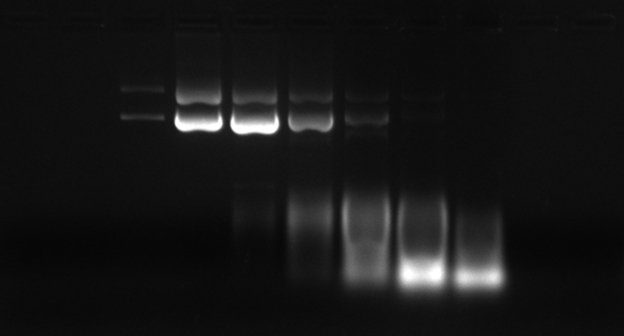
\includegraphics[width=6.3cm]{cort2.jpg}};

\node[white, above, font = \normalsize] at (5.400, 1.9) { 1};
\node[white, above, font = \normalsize] at (6.000, 1.9) { 2};
\node[white, above, font = \normalsize] at (6.600, 1.9) { 3};
\node[white, above, font = \normalsize] at (7.200, 1.9) { 4};
\node[white, above, font = \normalsize] at (7.850, 1.9) { 5};
\node[white, above, font = \normalsize] at (8.475, 1.9) { 6};
\node[white, above, font = \normalsize] at (9.150, 1.9) { 7};
\node[white, above, font = \normalsize] at (9.750, 1.9) { 8};
\node[white, above, font = \normalsize] at (10.35, 1.9) { 9};
\node[white, above, font = \normalsize] at (11.00, 1.9) {10};
\node[white, above, font = \normalsize] at (11.70, 1.9) {11};

\end{tikzpicture}
    \caption[Análise do lisado centrifugado com o gel Sephacryl S-1000.]{Análise do lisado centrifugado obtido após lise alcalina de \ecoli\ contendo o plasmídeo \pVAX. a) Perfil cromatográfico do lisado no gel Sephacryl S-1000 SF (SEC); b) Análise por HIC-HPLC das frações 5, 7, 9 e 10, recolhidas durante o ensaio de SEC. c) Análise por eletroforese das frações recolhidas durante o ensaio de SEC.}
    \label{fig:s1000}
\end{figure} 

Foi utilizado um procedimento semelhante para caracterizar o lisado com o gel Sephacryl S-100 HR. Os resultados obtidos encontram-se na figura~\ref{fig:s100}. É possível verificar que os ácidos nucleicos de maior massa molecular (pDNA e HMw\,RNA) não são retidos pelo gel e eluem em conjunto na fração 4. Para o LMw\,RNA observa-se uma ligeira retenção, sendo recolhido nas frações 4 e 5. Parte do material proteico é significativamente retido pelo gel. Observa-se a existência de uma elevada dispersividade de massas moleculares das proteínas presentes visto que estas são detetadas nas frações 5--12, cobrindo quase na totalidade o intervalo de fracionamento do gel. Pela análise dos cromatogramas de HIC (figura~\ref{fig:s100}~b), pode-se verificar que o RNA elui na região 3. De facto, apenas para as frações que contêm ácidos nucleios (frações 4--5) existe um valor de absorvância significativo nesta região e para estas frações não se deteta uma absorvância significativa na região 2.\index{proteínas!SEC}\index{proteínas!quantificação|see{BCA}}        
\begin{figure}[!t]
    \centering
    \begin{tikzpicture}[scale = 0.9]
%\draw[help lines] (0cm, 0cm) grid (17cm, 14cm);

\node[font = \large, below] at (1.5, 14) {a)};
\node[font = \large, below] at (1.5, 8.5) {b)};
\node[font = \large, below] at (1.5, 2.5) {c)};

\draw (12.1, 1.4) -- (12.25, 1.4) -- (12.35, 1.8) -- (12.5, 1.8)  node[right] {pDNA\,(oc)};
\draw (12.1, 1.1) -- (12.5, 1.1) node[right] {pDNA\,(sc)};
\draw (12.1, -0.1) -- (12.5, -0.1) node[right] {HMw\,RNA};
\draw (12.1, -0.95) -- (12.5, -0.95) node[right] {LMw\,RNA};

\node[below left, align = right] at (12.75, 13.75) {Sephacryl \\ S-100 HR};

\node[below left, font = \scriptsize] at (6, 7) {HIC};
\node[below left, font = \scriptsize] at (10, 7) {HIC};
\node[below left, font = \scriptsize] at (14, 7) {HIC};

\draw[dashed] (4.7, 9) -- (4.7, 10);
\node[above, font = \scriptsize] at (4.95, 10) {1};
\draw[dashed] (5.2, 9) -- (5.2, 10);
\node[above, font = \scriptsize] at (5.45, 10) {2};
\draw[dashed] (5.699, 9) -- (5.699, 10);
\node[above, font = \scriptsize] at (5.95, 10) {3};
\draw[dashed] (6.199, 9) -- (6.199, 10);
\node[above, font = \scriptsize] at (6.45, 10) {4};
\draw[dashed] (6.699, 9) -- (6.699, 10);
\node[above, font = \scriptsize] at (6.95, 10) {5};
\draw[dashed] (7.199, 9) -- (7.199, 10);
\node[above, font = \scriptsize] at (7.45, 10) {6};
\draw[dashed] (7.699, 9) -- (7.699, 10);
\node[above, font = \scriptsize] at (7.95, 10) {7};
\draw[dashed] (8.199, 9) -- (8.199, 10);
\node[above, font = \scriptsize] at (8.45, 10) {8};
\draw[dashed] (8.699, 9) -- (8.699, 10);
\node[above, font = \scriptsize] at (8.95, 10) {9};
\draw[dashed] (9.199, 9) -- (9.199, 10);
\node[above, font = \scriptsize] at (9.45, 10) {10};
\draw[dashed] (9.699, 9) -- (9.699, 10);
\node[above, font = \scriptsize] at (9.95, 10) {11};
\draw[dashed] (10.199, 9) -- (10.199, 10);

\draw[dashed] (6.199, 9) -- (3, 7) (6.699, 9) -- (6, 7);
\draw[dashed] (6.699, 9) -- (7, 7) (7.199, 9) -- (10, 7);
\draw[dashed] (8.199, 9) -- (11, 7) (8.699, 9) -- (14, 7);


\begin{axis}[%
xlabel style = {fill = white},
x tick label style = {fill = white},
width=9cm,
height=5cm,
scale only axis,
axis y line* = left,
xmin=-5,
xmax=85,
xlabel={$V_{\mr{R}}$\,[mL]},
% ymin=-500,
% ymax=3000,
ylabel={Absorvância 260\,nm [AU]},
at={(4cm, 9cm)},
anchor=south west,
ylabel near ticks
% legend style={at={(1.03,0.5)},legend columns=1,anchor=west,font=\scriptsize,draw=black,fill=white,legend cell align=left}
]
\addplot[
color=black,
solid
]
table[row sep=crcr]{
0.00000 0.00000\\
0.08000 0.00001\\
0.16000 0.00001\\
0.24000 0.00006\\
0.32000 0.00000\\
0.40000 0.00009\\
0.48000 0.00009\\
0.56000 0.00011\\
0.64000 0.00006\\
0.72000 0.00011\\
0.80000 0.00019\\
0.88000 0.00012\\
0.96000 0.00013\\
1.04000 0.00011\\
1.12000 0.00014\\
1.20000 0.00019\\
1.28000 0.00016\\
1.36000 0.00010\\
1.44000 0.00011\\
1.52000 0.00008\\
1.60000 0.00020\\
1.68000 0.00019\\
1.76000 0.00018\\
1.84000 0.00017\\
1.92000 0.00014\\
2.00000 0.00020\\
2.08000 0.00021\\
2.16000 0.00021\\
2.24000 0.00024\\
2.32000 0.00017\\
2.40000 0.00016\\
2.48000 0.00033\\
2.56000 0.00023\\
2.64000 0.00020\\
2.72000 0.00030\\
2.80000 0.00028\\
2.88000 0.00031\\
2.96000 0.00029\\
3.04000 0.00031\\
3.12000 0.00031\\
3.20000 0.00027\\
3.28000 0.00033\\
3.36000 0.00029\\
3.44000 0.00033\\
3.52000 0.00037\\
3.60000 0.00032\\
3.68000 0.00037\\
3.76000 0.00040\\
3.84000 0.00041\\
3.92000 0.00043\\
4.00000 0.00041\\
4.08000 0.00040\\
4.16000 0.00041\\
4.24000 0.00047\\
4.32000 0.00041\\
4.40000 0.00045\\
4.48000 0.00050\\
4.56000 0.00045\\
4.64000 0.00047\\
4.72000 0.00051\\
4.80000 0.00052\\
4.88000 0.00052\\
4.96000 0.00058\\
5.04000 0.00056\\
5.12000 0.00054\\
5.20000 0.00056\\
5.28000 0.00053\\
5.36000 0.00057\\
5.44000 0.00059\\
5.52000 0.00059\\
5.60000 0.00063\\
5.68000 0.00064\\
5.76000 0.00058\\
5.84000 0.00061\\
5.92000 0.00065\\
6.00000 0.00064\\
6.08000 0.00061\\
6.16000 0.00065\\
6.24000 0.00067\\
6.32000 0.00072\\
6.40000 0.00068\\
6.48000 0.00075\\
6.56000 0.00072\\
6.64000 0.00072\\
6.72000 0.00076\\
6.80000 0.00078\\
6.88000 0.00078\\
6.96000 0.00083\\
7.04000 0.00075\\
7.12000 0.00073\\
7.20000 0.00073\\
7.28000 0.00071\\
7.36000 0.00072\\
7.44000 0.00074\\
7.52000 0.00075\\
7.60000 0.00077\\
7.68000 0.00075\\
7.76000 0.00077\\
7.84000 0.00075\\
7.92000 0.00071\\
8.00000 0.00073\\
8.08000 0.00073\\
8.16000 0.00076\\
8.24000 0.00074\\
8.32000 0.00083\\
8.40000 0.00080\\
8.48000 0.00087\\
8.56000 0.00084\\
8.64000 0.00090\\
8.72000 0.00094\\
8.80000 0.00090\\
8.88000 0.00090\\
8.96000 0.00093\\
9.04000 0.00095\\
9.12000 0.00095\\
9.20000 0.00100\\
9.28000 0.00106\\
9.36000 0.00101\\
9.44000 0.00106\\
9.52000 0.00110\\
9.60000 0.00106\\
9.68000 0.00110\\
9.76000 0.00110\\
9.84000 0.00114\\
9.92000 0.00110\\
10.00000 0.00109\\
10.08000 0.00112\\
10.16000 0.00113\\
10.24000 0.00119\\
10.32000 0.00116\\
10.40000 0.00114\\
10.48000 0.00116\\
10.56000 0.00122\\
10.64000 0.00122\\
10.72000 0.00125\\
10.80000 0.00123\\
10.88000 0.00127\\
10.96000 0.00125\\
11.04000 0.00122\\
11.12000 0.00122\\
11.20000 0.00127\\
11.28000 0.00130\\
11.36000 0.00136\\
11.44000 0.00141\\
11.52000 0.00134\\
11.60100 0.00134\\
11.68100 0.00134\\
11.76100 0.00131\\
11.84100 0.00135\\
11.92100 0.00130\\
12.00100 0.00128\\
12.08100 0.00127\\
12.16100 0.00132\\
12.24100 0.00144\\
12.32100 0.00135\\
12.40100 0.00137\\
12.48100 0.00138\\
12.56100 0.00135\\
12.64100 0.00135\\
12.72100 0.00138\\
12.80100 0.00139\\
12.88100 0.00133\\
12.96100 0.00138\\
13.04100 0.00132\\
13.12100 0.00135\\
13.20100 0.00141\\
13.28100 0.00144\\
13.36100 0.00146\\
13.44100 0.00149\\
13.52100 0.00160\\
13.60100 0.00159\\
13.68100 0.00168\\
13.76100 0.00170\\
13.84100 0.00166\\
13.92100 0.00170\\
14.00100 0.00168\\
14.08100 0.00179\\
14.16100 0.00181\\
14.24100 0.00176\\
14.32100 0.00179\\
14.40100 0.00177\\
14.48100 0.00169\\
14.56100 0.00176\\
14.64100 0.00168\\
14.72100 0.00163\\
14.80100 0.00157\\
14.88100 0.00154\\
14.96100 0.00153\\
15.04100 0.00153\\
15.12100 0.00152\\
15.20100 0.00141\\
15.28100 0.00137\\
15.36100 0.00134\\
15.44100 0.00133\\
15.52100 0.00124\\
15.60100 0.00125\\
15.68100 0.00120\\
15.76100 0.00127\\
15.84100 0.00122\\
15.92100 0.00138\\
16.00100 0.00146\\
16.08100 0.00164\\
16.16100 0.00201\\
16.24100 0.00275\\
16.32100 0.00418\\
16.40100 0.00656\\
16.48100 0.01051\\
16.56100 0.01676\\
16.64100 0.02657\\
16.72100 0.04156\\
16.80100 0.06412\\
16.88100 0.09724\\
16.96100 0.14617\\
17.04100 0.21905\\
17.12100 0.32466\\
17.20100 0.47598\\
17.28100 0.69364\\
17.36100 0.99170\\
17.44100 1.38444\\
17.52100 1.87552\\
17.60100 2.43699\\
17.68100 3.09102\\
17.76100 4.05370\\
17.84100 4.64702\\
17.92100 4.81992\\
18.00100 4.79184\\
18.08100 4.79751\\
18.16100 4.84212\\
18.24100 4.80077\\
18.32100 4.84815\\
18.40100 4.85386\\
18.48100 4.82350\\
18.56100 4.77945\\
18.64100 4.85318\\
18.72100 4.79380\\
18.80100 4.80076\\
18.88100 4.79666\\
18.96100 4.82594\\
19.04100 4.84803\\
19.12100 4.80284\\
19.20100 4.80892\\
19.28100 4.79035\\
19.36100 4.76371\\
19.44100 4.71055\\
19.52100 4.62117\\
19.60100 4.41841\\
19.68100 3.95133\\
19.76100 3.44111\\
19.84100 3.16318\\
19.92100 2.91691\\
20.00100 2.69867\\
20.08100 2.50509\\
20.16100 2.34510\\
20.24100 2.19620\\
20.32100 2.07252\\
20.40100 1.95319\\
20.48100 1.85028\\
20.56100 1.76001\\
20.64100 1.67839\\
20.72100 1.59916\\
20.80100 1.53351\\
20.88100 1.47017\\
20.96100 1.41442\\
21.04100 1.35965\\
21.12100 1.31460\\
21.20100 1.27519\\
21.28100 1.24127\\
21.36100 1.21054\\
21.44100 1.18744\\
21.52100 1.16651\\
21.60100 1.15146\\
21.68100 1.14168\\
21.76100 1.13581\\
21.84100 1.13465\\
21.92100 1.13758\\
22.00100 1.14323\\
22.08100 1.15154\\
22.16100 1.16169\\
22.24100 1.17403\\
22.32100 1.18688\\
22.40100 1.19991\\
22.48100 1.21289\\
22.56100 1.22413\\
22.64100 1.23473\\
22.72100 1.24253\\
22.80100 1.24798\\
22.88100 1.25017\\
22.96100 1.24898\\
23.04100 1.24439\\
23.12100 1.23572\\
23.20100 1.22331\\
23.28100 1.20668\\
23.36100 1.18549\\
23.44100 1.16102\\
23.52100 1.13340\\
23.60100 1.10285\\
23.68100 1.06874\\
23.76100 1.03170\\
23.84100 0.99320\\
23.92100 0.95382\\
24.00100 0.91329\\
24.08100 0.87201\\
24.16100 0.83015\\
24.24100 0.78931\\
24.32100 0.74891\\
24.40100 0.70950\\
24.48100 0.67159\\
24.56100 0.63455\\
24.64100 0.59924\\
24.72100 0.56602\\
24.80100 0.53411\\
24.88100 0.50430\\
24.96100 0.47555\\
25.04100 0.44885\\
25.12100 0.42396\\
25.20100 0.40141\\
25.28100 0.37963\\
25.36100 0.35978\\
25.44100 0.34112\\
25.52100 0.32372\\
25.60100 0.30774\\
25.68100 0.29318\\
25.76100 0.27935\\
25.84100 0.26655\\
25.92100 0.25469\\
26.00100 0.24350\\
26.08100 0.23314\\
26.16100 0.22313\\
26.24100 0.21399\\
26.32100 0.20520\\
26.40100 0.19742\\
26.48100 0.18975\\
26.56100 0.18265\\
26.64100 0.17557\\
26.72100 0.16898\\
26.80100 0.16288\\
26.88100 0.15713\\
26.96100 0.15146\\
27.04100 0.14647\\
27.12100 0.14124\\
27.20100 0.13626\\
27.28100 0.13150\\
27.36100 0.12710\\
27.44100 0.12284\\
27.52100 0.11900\\
27.60100 0.11499\\
27.68100 0.11127\\
27.76100 0.10750\\
27.84100 0.10395\\
27.92100 0.10058\\
28.00100 0.09738\\
28.08100 0.09423\\
28.16100 0.09118\\
28.24100 0.08834\\
28.32100 0.08550\\
28.40100 0.08279\\
28.48100 0.08019\\
28.56100 0.07759\\
28.64100 0.07527\\
28.72100 0.07294\\
28.80100 0.07070\\
28.88100 0.06840\\
28.96100 0.06623\\
29.04100 0.06420\\
29.12100 0.06220\\
29.20100 0.06031\\
29.28100 0.05841\\
29.36100 0.05660\\
29.44100 0.05489\\
29.52100 0.05320\\
29.60100 0.05146\\
29.68100 0.04987\\
29.76100 0.04837\\
29.84100 0.04691\\
29.92100 0.04550\\
30.00100 0.04420\\
30.08100 0.04283\\
30.16100 0.04154\\
30.24100 0.04035\\
30.32100 0.03924\\
30.40100 0.03809\\
30.48100 0.03702\\
30.56100 0.03599\\
30.64100 0.03496\\
30.72100 0.03409\\
30.80100 0.03326\\
30.88100 0.03246\\
30.96100 0.03172\\
31.04100 0.03109\\
31.12100 0.03047\\
31.20100 0.02996\\
31.28100 0.02954\\
31.36100 0.02925\\
31.44100 0.02906\\
31.52100 0.02897\\
31.60100 0.02905\\
31.68100 0.02929\\
31.76100 0.02965\\
31.84100 0.03026\\
31.92100 0.03104\\
32.00100 0.03209\\
32.08100 0.03332\\
32.16100 0.03472\\
32.24100 0.03643\\
32.32100 0.03834\\
32.40100 0.04050\\
32.48100 0.04291\\
32.56100 0.04553\\
32.64100 0.04830\\
32.72100 0.05123\\
32.80100 0.05423\\
32.88100 0.05745\\
32.96100 0.06071\\
33.04100 0.06409\\
33.12100 0.06747\\
33.20100 0.07092\\
33.28100 0.07441\\
33.36100 0.07785\\
33.44100 0.08125\\
33.52100 0.08480\\
33.60100 0.08821\\
33.68100 0.09171\\
33.76100 0.09523\\
33.84100 0.09898\\
33.92100 0.10291\\
34.00100 0.10721\\
34.08100 0.11220\\
34.16100 0.11813\\
34.24100 0.12499\\
34.32100 0.13250\\
34.40100 0.14051\\
34.48100 0.14892\\
34.56100 0.15749\\
34.64100 0.16638\\
34.72200 0.17515\\
34.80200 0.18342\\
34.88200 0.19039\\
34.96200 0.19672\\
35.04200 0.20203\\
35.12200 0.20653\\
35.20200 0.21046\\
35.28200 0.21393\\
35.36200 0.21696\\
35.44200 0.21971\\
35.52200 0.22233\\
35.60200 0.22474\\
35.68200 0.22702\\
35.76200 0.22930\\
35.84200 0.23158\\
35.92200 0.23389\\
36.00200 0.23623\\
36.08200 0.23876\\
36.16200 0.24132\\
36.24200 0.24408\\
36.32200 0.24698\\
36.40200 0.24990\\
36.48200 0.25303\\
36.56200 0.25628\\
36.64200 0.25959\\
36.72200 0.26300\\
36.80200 0.26656\\
36.88200 0.27013\\
36.96200 0.27382\\
37.04200 0.27755\\
37.12200 0.28132\\
37.20200 0.28516\\
37.28200 0.28903\\
37.36200 0.29295\\
37.44200 0.29695\\
37.52200 0.30070\\
37.60200 0.30456\\
37.68200 0.30833\\
37.76200 0.31217\\
37.84200 0.31583\\
37.92200 0.31954\\
38.00200 0.32309\\
38.08200 0.32651\\
38.16200 0.33012\\
38.24200 0.33413\\
38.32200 0.33802\\
38.40200 0.34123\\
38.48200 0.34316\\
38.56200 0.34597\\
38.64200 0.34835\\
38.72200 0.35017\\
38.80200 0.35157\\
38.88200 0.35477\\
38.96200 0.35773\\
39.04200 0.35900\\
39.12200 0.36235\\
39.20200 0.36553\\
39.28200 0.36771\\
39.36200 0.36992\\
39.44200 0.37334\\
39.52200 0.37576\\
39.60200 0.37939\\
39.68200 0.38360\\
39.76200 0.38918\\
39.84200 0.39671\\
39.92200 0.40414\\
40.00200 0.41294\\
40.08200 0.42162\\
40.16200 0.43604\\
40.24200 0.44963\\
40.32200 0.46686\\
40.40200 0.48825\\
40.48200 0.50942\\
40.56200 0.54051\\
40.64200 0.57246\\
40.72200 0.60813\\
40.80200 0.64141\\
40.88200 0.67368\\
40.96200 0.70530\\
41.04200 0.73307\\
41.12200 0.75830\\
41.20200 0.77737\\
41.28200 0.79481\\
41.36200 0.80967\\
41.44200 0.82235\\
41.52200 0.83122\\
41.60200 0.83778\\
41.68200 0.84269\\
41.76200 0.84633\\
41.84200 0.84941\\
41.92200 0.85151\\
42.00200 0.85097\\
42.08200 0.85066\\
42.16200 0.84861\\
42.24200 0.84418\\
42.32200 0.83982\\
42.40200 0.83564\\
42.48200 0.83049\\
42.56200 0.82523\\
42.64200 0.81891\\
42.72200 0.81364\\
42.80200 0.80821\\
42.88200 0.80391\\
42.96200 0.79899\\
43.04200 0.79493\\
43.12200 0.79049\\
43.20200 0.78672\\
43.28200 0.78285\\
43.36200 0.77964\\
43.44200 0.77623\\
43.52200 0.77283\\
43.60200 0.76823\\
43.68200 0.76171\\
43.76200 0.75505\\
43.84200 0.74510\\
43.92200 0.73413\\
44.00200 0.72193\\
44.08200 0.70882\\
44.16200 0.69520\\
44.24200 0.68086\\
44.32200 0.66668\\
44.40200 0.65235\\
44.48200 0.63907\\
44.56200 0.62633\\
44.64200 0.61538\\
44.72200 0.60378\\
44.80200 0.59276\\
44.88200 0.58141\\
44.96200 0.57135\\
45.04200 0.56135\\
45.12200 0.55251\\
45.20200 0.54343\\
45.28200 0.53557\\
45.36200 0.52873\\
45.44200 0.52253\\
45.52200 0.51713\\
45.60200 0.51315\\
45.68200 0.50975\\
45.76200 0.50696\\
45.84200 0.50579\\
45.92200 0.50487\\
46.00200 0.50391\\
46.08200 0.50288\\
46.16200 0.50240\\
46.24200 0.50146\\
46.32200 0.50065\\
46.40200 0.49904\\
46.48200 0.49757\\
46.56200 0.49505\\
46.64200 0.49241\\
46.72200 0.48931\\
46.80200 0.48568\\
46.88200 0.48082\\
46.96200 0.47627\\
47.04200 0.47036\\
47.12200 0.46432\\
47.20200 0.45838\\
47.28200 0.45206\\
47.36200 0.44376\\
47.44200 0.43379\\
47.52200 0.42195\\
47.60200 0.40896\\
47.68200 0.39560\\
47.76200 0.38300\\
47.84200 0.37117\\
47.92200 0.36069\\
48.00200 0.35132\\
48.08200 0.34309\\
48.16200 0.33594\\
48.24200 0.32963\\
48.32200 0.32413\\
48.40200 0.31923\\
48.48200 0.31481\\
48.56200 0.31066\\
48.64200 0.30685\\
48.72200 0.30311\\
48.80200 0.29953\\
48.88200 0.29609\\
48.96200 0.29268\\
49.04200 0.28930\\
49.12200 0.28599\\
49.20200 0.28258\\
49.28200 0.27925\\
49.36200 0.27595\\
49.44200 0.27268\\
49.52200 0.26944\\
49.60200 0.26623\\
49.68200 0.26300\\
49.76200 0.25993\\
49.84200 0.25689\\
49.92200 0.25385\\
50.00200 0.25086\\
50.08200 0.24806\\
50.16200 0.24526\\
50.24200 0.24265\\
50.32200 0.24008\\
50.40200 0.23755\\
50.48200 0.23507\\
50.56200 0.23260\\
50.64200 0.23018\\
50.72200 0.22788\\
50.80200 0.22548\\
50.88200 0.22311\\
50.96200 0.22069\\
51.04200 0.21819\\
51.12200 0.21579\\
51.20200 0.21323\\
51.28200 0.21062\\
51.36200 0.20793\\
51.44200 0.20515\\
51.52200 0.20230\\
51.60200 0.19934\\
51.68200 0.19623\\
51.76200 0.19310\\
51.84200 0.18986\\
51.92200 0.18648\\
52.00200 0.18304\\
52.08200 0.17948\\
52.16200 0.17585\\
52.24200 0.17214\\
52.32200 0.16823\\
52.40200 0.16437\\
52.48200 0.16041\\
52.56200 0.15647\\
52.64200 0.15242\\
52.72200 0.14837\\
52.80200 0.14416\\
52.88200 0.14012\\
52.96200 0.13601\\
53.04200 0.13194\\
53.12200 0.12781\\
53.20200 0.12383\\
53.28200 0.11988\\
53.36200 0.11591\\
53.44200 0.11204\\
53.52200 0.10826\\
53.60200 0.10463\\
53.68200 0.10105\\
53.76200 0.09758\\
53.84200 0.09435\\
53.92200 0.09120\\
54.00200 0.08841\\
54.08200 0.08576\\
54.16200 0.08346\\
54.24200 0.08174\\
54.32200 0.08095\\
54.40200 0.08260\\
54.48200 0.08933\\
54.56200 0.10543\\
54.64200 0.13446\\
54.72200 0.17449\\
54.80200 0.21140\\
54.88200 0.24212\\
54.96200 0.26351\\
55.04200 0.27632\\
55.12200 0.28393\\
55.20200 0.28843\\
55.28200 0.29072\\
55.36200 0.29061\\
55.44200 0.28951\\
55.52200 0.28722\\
55.60200 0.28514\\
55.68200 0.28184\\
55.76200 0.27796\\
55.84200 0.27358\\
55.92200 0.26815\\
56.00200 0.26171\\
56.08200 0.25388\\
56.16200 0.24578\\
56.24200 0.23737\\
56.32200 0.22906\\
56.40200 0.22062\\
56.48200 0.21219\\
56.56200 0.20290\\
56.64200 0.19276\\
56.72200 0.18195\\
56.80200 0.17065\\
56.88200 0.15984\\
56.96200 0.14925\\
57.04200 0.13925\\
57.12200 0.12982\\
57.20200 0.12080\\
57.28200 0.11214\\
57.36200 0.10403\\
57.44200 0.09660\\
57.52200 0.08977\\
57.60200 0.08355\\
57.68200 0.07785\\
57.76200 0.07258\\
57.84300 0.06760\\
57.92300 0.06307\\
58.00300 0.05905\\
58.08300 0.05517\\
58.16300 0.05150\\
58.24300 0.04830\\
58.32300 0.04531\\
58.40300 0.04244\\
58.48300 0.03986\\
58.56300 0.03742\\
58.64300 0.03514\\
58.72300 0.03309\\
58.80300 0.03109\\
58.88300 0.02928\\
58.96300 0.02755\\
59.04300 0.02606\\
59.12300 0.02457\\
59.20300 0.02326\\
59.28300 0.02204\\
59.36300 0.02088\\
59.44300 0.01992\\
59.52300 0.01893\\
59.60300 0.01795\\
59.68300 0.01715\\
59.76300 0.01633\\
59.84300 0.01565\\
59.92300 0.01500\\
60.00300 0.01445\\
60.08300 0.01386\\
60.16300 0.01331\\
60.24300 0.01291\\
60.32300 0.01258\\
60.40300 0.01218\\
60.48300 0.01183\\
60.56300 0.01156\\
60.64300 0.01128\\
60.72300 0.01111\\
60.80300 0.01090\\
60.88300 0.01072\\
60.96300 0.01047\\
61.04300 0.01039\\
61.12300 0.01023\\
61.20300 0.01017\\
61.28300 0.01006\\
61.36300 0.01003\\
61.44300 0.00990\\
61.52300 0.00984\\
61.60300 0.00980\\
61.68300 0.00978\\
61.76300 0.00977\\
61.84300 0.00971\\
61.92300 0.00966\\
62.00300 0.00959\\
62.08300 0.00961\\
62.16300 0.00962\\
62.24300 0.00956\\
62.32300 0.00947\\
62.40300 0.00950\\
62.48300 0.00948\\
62.56300 0.00938\\
62.64300 0.00933\\
62.72300 0.00930\\
62.80300 0.00922\\
62.88300 0.00914\\
62.96300 0.00917\\
63.04300 0.00902\\
63.12300 0.00896\\
63.20300 0.00892\\
63.28300 0.00880\\
63.36300 0.00878\\
63.44300 0.00869\\
63.52300 0.00856\\
63.60300 0.00844\\
63.68300 0.00837\\
63.76300 0.00826\\
63.84300 0.00811\\
63.92300 0.00814\\
64.00300 0.00792\\
64.08300 0.00780\\
64.16300 0.00766\\
64.24300 0.00750\\
64.32300 0.00748\\
64.40300 0.00734\\
64.48300 0.00721\\
64.56300 0.00715\\
64.64300 0.00696\\
64.72300 0.00688\\
64.80300 0.00673\\
64.88300 0.00653\\
64.96300 0.00649\\
65.04300 0.00630\\
65.12300 0.00623\\
65.20300 0.00614\\
65.28300 0.00598\\
65.36300 0.00582\\
65.44300 0.00570\\
65.52300 0.00558\\
65.60300 0.00549\\
65.68300 0.00542\\
65.76300 0.00523\\
65.84300 0.00516\\
65.92300 0.00503\\
66.00300 0.00493\\
66.08300 0.00490\\
66.16300 0.00470\\
66.24300 0.00463\\
66.32300 0.00455\\
66.40300 0.00446\\
66.48300 0.00437\\
66.56300 0.00431\\
66.64300 0.00419\\
66.72300 0.00410\\
66.80300 0.00403\\
66.88300 0.00394\\
66.96300 0.00391\\
67.04300 0.00382\\
67.12300 0.00374\\
67.20300 0.00364\\
67.28300 0.00359\\
67.36300 0.00359\\
67.44300 0.00345\\
67.52300 0.00350\\
67.60300 0.00345\\
67.68300 0.00343\\
67.76300 0.00338\\
67.84300 0.00333\\
67.92300 0.00327\\
68.00300 0.00322\\
68.08300 0.00318\\
68.16300 0.00313\\
68.24300 0.00312\\
68.32300 0.00313\\
68.40300 0.00313\\
68.48300 0.00310\\
68.56300 0.00308\\
68.64300 0.00303\\
68.72300 0.00302\\
68.80300 0.00299\\
68.88300 0.00301\\
68.96300 0.00298\\
69.04300 0.00295\\
69.12300 0.00296\\
69.20300 0.00298\\
69.28300 0.00287\\
69.36300 0.00290\\
69.44300 0.00287\\
69.52300 0.00285\\
69.60300 0.00287\\
69.68300 0.00285\\
69.76300 0.00287\\
69.84300 0.00283\\
69.92300 0.00278\\
70.00300 0.00278\\
70.08300 0.00286\\
70.16300 0.00283\\
70.24300 0.00280\\
70.32300 0.00277\\
70.40300 0.00266\\
70.48300 0.00265\\
70.56300 0.00265\\
70.64300 0.00268\\
70.72300 0.00264\\
70.80300 0.00269\\
70.88300 0.00266\\
70.96300 0.00262\\
71.04300 0.00262\\
71.12300 0.00256\\
71.20300 0.00255\\
71.28300 0.00253\\
71.36300 0.00257\\
71.44300 0.00253\\
71.52300 0.00253\\
71.60300 0.00244\\
71.68300 0.00241\\
71.76300 0.00239\\
71.84300 0.00239\\
71.92300 0.00238\\
72.00300 0.00237\\
72.08300 0.00231\\
72.16300 0.00234\\
72.24300 0.00224\\
72.32300 0.00231\\
72.40300 0.00226\\
72.48300 0.00220\\
72.56300 0.00220\\
72.64300 0.00215\\
72.72300 0.00216\\
72.80300 0.00209\\
72.88300 0.00213\\
72.96300 0.00207\\
73.04300 0.00208\\
73.12300 0.00207\\
73.20300 0.00196\\
73.28300 0.00196\\
73.36300 0.00193\\
73.44300 0.00194\\
73.52300 0.00187\\
73.60300 0.00187\\
73.68300 0.00180\\
73.76300 0.00181\\
73.84300 0.00182\\
73.92300 0.00183\\
74.00300 0.00181\\
74.08300 0.00174\\
74.16300 0.00170\\
74.24300 0.00174\\
74.32300 0.00174\\
74.40300 0.00167\\
74.48300 0.00165\\
74.56300 0.00163\\
74.64300 0.00160\\
74.72300 0.00160\\
74.80300 0.00160\\
74.88300 0.00162\\
74.96300 0.00152\\
75.04300 0.00153\\
75.12300 0.00152\\
75.20300 0.00148\\
75.28300 0.00143\\
75.36300 0.00138\\
75.44300 0.00141\\
75.52300 0.00141\\
75.60300 0.00141\\
75.68300 0.00139\\
75.76300 0.00139\\
75.84300 0.00137\\
75.92300 0.00145\\
76.00300 0.00131\\
76.08300 0.00135\\
76.16300 0.00134\\
76.24300 0.00131\\
76.32300 0.00129\\
76.40300 0.00126\\
76.48300 0.00128\\
76.56300 0.00125\\
76.64300 0.00125\\
76.72300 0.00125\\
76.80300 0.00131\\
76.88300 0.00125\\
76.96300 0.00126\\
};
\end{axis}

\begin{axis}[%
width=9cm,
height=5cm,
scale only axis,
at={(4cm, 9cm)},
anchor=south west,
xmin=-5,
xmax=85,
axis y line* = right,
axis x line = none,
% ymin=-500,
% ymax=3000,
ylabel={Proteína total [\micro g/mL]},
ylabel near ticks
% legend style={at={(1.03,0.5)},legend columns=1,anchor=west,font=\scriptsize,draw=black,fill=white,legend cell align=left}
]
\addplot+[const plot mark mid, color = black, mark options={fill=black}]
coordinates{
(4.500000, 0.806584)
(9.500000, 0.000000)
(14.50000, 1.411523)
(19.50000, 2.621399)
(24.50000, 7.057613)
(29.50000, 5.646091)
(34.50000, 12.70370)
(39.50000, 50.41152)
(44.50000, 49.00000)
(49.50000, 14.31687)
(54.50000, 15.93004)
(59.50000, 6.654321)
(64.50000, 2.218107)
(69.50000, 1.411523)
(74.50000, 2.218107)
};
\end{axis}

\begin{axis}[%
width=3cm,
height=3cm,
scale only axis,
% xmin=-5,
% xmax=85,
xlabel={$V_{\mr{R}}$\,[mL]},
% ymin=-500,
% ymax=100,
% ylabel={},
at={(3cm, 4cm)},
anchor=south west,
% legend style={at={(1.03,0.5)},legend columns=1,anchor=west,font=\scriptsize,draw=black,fill=white,legend cell align=left}
]
\addplot[
color=black,
solid
]
table[row sep=crcr]{
0.00000 -0.01400\\
0.00800 -0.01500\\
0.01700 -0.01800\\
0.02500 -0.02100\\
0.03300 -0.01700\\
0.04200 -0.00800\\
0.05000 -0.00300\\
0.05800 0.01200\\
0.06700 0.01600\\
0.07500 0.01800\\
0.08300 0.02100\\
0.09200 0.02400\\
0.10000 0.02200\\
0.10800 0.01900\\
0.11600 0.01400\\
0.12500 0.00600\\
0.13300 0.00000\\
0.14100 -0.00100\\
0.15000 -0.00600\\
0.15800 -0.00300\\
0.16600 -0.00200\\
0.17500 -0.00100\\
0.18300 -0.00300\\
0.19100 -0.00700\\
0.20000 -0.00700\\
0.20800 -0.00900\\
0.21600 -0.02000\\
0.22500 -0.03200\\
0.23300 -0.04100\\
0.24100 -0.04400\\
0.25000 -0.05100\\
0.25800 -0.04300\\
0.26600 -0.03800\\
0.27500 -0.03200\\
0.28300 -0.02700\\
0.29100 -0.02000\\
0.29900 -0.02700\\
0.30800 -0.03000\\
0.31600 -0.03600\\
0.32400 -0.04400\\
0.33300 -0.05100\\
0.34100 -0.05000\\
0.34900 -0.04200\\
0.35800 -0.03200\\
0.36600 -0.02600\\
0.37400 -0.02200\\
0.38300 -0.01800\\
0.39100 -0.02000\\
0.39900 -0.02400\\
0.40800 -0.02800\\
0.41600 -0.02800\\
0.42400 -0.02900\\
0.43300 -0.03300\\
0.44100 -0.03300\\
0.44900 -0.03100\\
0.45800 -0.02700\\
0.46600 -0.02100\\
0.47400 -0.02100\\
0.48300 -0.02600\\
0.49100 -0.03300\\
0.49900 -0.03300\\
0.50700 -0.04000\\
0.51600 -0.04200\\
0.52400 -0.03600\\
0.53200 -0.03000\\
0.54100 -0.03600\\
0.54900 -0.03300\\
0.55700 -0.02500\\
0.56600 -0.02400\\
0.57400 -0.02300\\
0.58200 -0.01900\\
0.59100 -0.01800\\
0.59900 -0.02400\\
0.60700 -0.01000\\
0.61600 0.10500\\
0.62400 0.48900\\
0.63200 1.41100\\
0.64100 3.24000\\
0.64900 7.08100\\
0.65700 12.66400\\
0.66600 19.53600\\
0.67400 26.69300\\
0.68200 33.19100\\
0.69000 38.59900\\
0.69900 41.65700\\
0.70700 42.42700\\
0.71500 41.57800\\
0.72400 39.55500\\
0.73200 36.79900\\
0.74000 33.84500\\
0.74900 30.72900\\
0.75700 27.65300\\
0.76500 24.85900\\
0.77400 22.41900\\
0.78200 20.29500\\
0.79000 18.41000\\
0.79900 16.81400\\
0.80700 15.51300\\
0.81500 14.37400\\
0.82400 13.33900\\
0.83200 12.39600\\
0.84000 11.56200\\
0.84900 10.72000\\
0.85700 9.86900\\
0.86500 9.04500\\
0.87400 8.25800\\
0.88200 7.50600\\
0.89000 6.80600\\
0.89800 6.19300\\
0.90700 5.63500\\
0.91500 5.14100\\
0.92300 4.70300\\
0.93200 4.30600\\
0.94000 3.96400\\
0.94800 3.67200\\
0.95700 3.42200\\
0.96500 3.20300\\
0.97300 3.00900\\
0.98200 2.83200\\
0.99000 2.67000\\
0.99800 2.52200\\
1.00700 2.38900\\
1.01500 2.26900\\
1.02300 2.16300\\
1.03200 2.07400\\
1.04000 1.99200\\
1.04800 1.94100\\
1.05700 1.93200\\
1.06500 1.98900\\
1.07300 2.06700\\
1.08100 2.08600\\
1.09000 1.96700\\
1.09800 1.65500\\
1.10600 1.12200\\
1.11500 0.46800\\
1.12300 -0.15600\\
1.13100 -0.56200\\
1.14000 -0.41100\\
1.14800 0.62200\\
1.15600 2.07000\\
1.16500 3.73200\\
1.17300 5.36600\\
1.18100 6.70400\\
1.19000 7.43600\\
1.19800 7.66600\\
1.20600 7.83600\\
1.21500 7.91200\\
1.22300 7.94900\\
1.23100 8.06600\\
1.24000 8.03500\\
1.24800 8.02000\\
1.25600 7.94300\\
1.26500 7.79300\\
1.27300 7.59800\\
1.28100 7.39700\\
1.28900 7.14900\\
1.29800 6.80000\\
1.30600 6.42800\\
1.31400 6.15200\\
1.32300 5.94100\\
1.33100 5.66100\\
1.33900 5.54800\\
1.34800 5.41700\\
1.35600 5.29200\\
1.36400 5.14300\\
1.37300 5.02400\\
1.38100 5.05700\\
1.38900 5.17700\\
1.39800 5.44200\\
1.40600 5.79000\\
1.41400 6.16000\\
1.42300 6.44900\\
1.43100 6.52800\\
1.43900 6.33100\\
1.44800 5.94100\\
1.45600 5.47700\\
1.46400 5.02500\\
1.47200 4.65100\\
1.48100 4.39800\\
1.48900 4.25700\\
1.49700 4.23500\\
1.50600 4.25800\\
1.51400 4.29400\\
1.52200 4.31800\\
1.53100 4.31200\\
1.53900 4.30800\\
1.54700 4.28600\\
1.55600 4.24900\\
1.56400 4.20700\\
1.57200 4.15900\\
1.58100 4.10100\\
1.58900 4.03600\\
1.59700 3.98100\\
1.60600 3.93300\\
1.61400 3.88600\\
1.62200 3.83900\\
1.63100 3.79700\\
1.63900 3.75300\\
1.64700 3.69600\\
1.65600 3.64600\\
1.66400 3.60200\\
1.67200 3.55500\\
1.68000 3.50400\\
1.68900 3.46100\\
1.69700 3.42900\\
1.70500 3.39800\\
1.71400 3.37400\\
1.72200 3.35900\\
1.73000 3.34800\\
1.73900 3.34500\\
1.74700 3.34000\\
1.75500 3.33700\\
1.76400 3.33800\\
1.77200 3.34000\\
1.78000 3.34200\\
1.78900 3.33700\\
1.79700 3.33600\\
1.80500 3.33900\\
1.81400 3.34300\\
1.82200 3.34700\\
1.83000 3.35700\\
1.83900 3.37300\\
1.84700 3.37800\\
1.85500 3.38000\\
1.86300 3.38900\\
1.87200 3.40400\\
1.88000 3.41000\\
1.88800 3.41800\\
1.89700 3.42100\\
1.90500 3.42500\\
1.91300 3.42700\\
1.92200 3.42400\\
1.93000 3.43000\\
1.93800 3.43600\\
1.94700 3.44100\\
1.95500 3.44200\\
1.96300 3.43900\\
1.97200 3.43800\\
1.98000 3.44000\\
1.98800 3.43600\\
1.99700 3.43800\\
2.00500 3.44200\\
2.01300 3.44700\\
2.02200 3.45500\\
2.03000 3.45500\\
2.03800 3.45700\\
2.04600 3.45700\\
2.05500 3.45600\\
2.06300 3.45600\\
2.07100 3.46300\\
2.08000 3.46400\\
2.08800 3.46200\\
2.09600 3.46500\\
2.10500 3.46100\\
2.11300 3.45000\\
2.12100 3.43600\\
2.13000 3.42400\\
2.13800 3.41100\\
2.14600 3.40300\\
2.15500 3.40000\\
2.16300 3.39900\\
2.17100 3.39600\\
2.18000 3.37800\\
2.18800 3.36400\\
2.19600 3.34200\\
2.20500 3.32800\\
2.21300 3.32500\\
2.22100 3.32800\\
2.23000 3.32300\\
2.23800 3.32100\\
2.24600 3.31700\\
2.25400 3.31100\\
2.26300 3.30500\\
2.27100 3.30200\\
2.27900 3.29200\\
2.28800 3.27300\\
2.29600 3.26600\\
2.30400 3.26400\\
2.31300 3.26200\\
2.32100 3.26500\\
2.32900 3.26600\\
2.33800 3.25200\\
2.34600 3.24500\\
2.35400 3.23400\\
2.36300 3.21800\\
2.37100 3.20800\\
2.37900 3.20400\\
2.38800 3.18900\\
2.39600 3.17600\\
2.40400 3.17100\\
2.41300 3.17000\\
2.42100 3.16000\\
2.42900 3.15000\\
2.43700 3.13900\\
2.44600 3.11900\\
2.45400 3.10000\\
2.46200 3.08500\\
2.47100 3.07300\\
2.47900 3.05700\\
2.48700 3.04300\\
2.49600 3.03600\\
2.50400 3.02900\\
2.51200 3.02000\\
2.52100 3.00900\\
2.52900 2.99300\\
2.53700 2.97700\\
2.54600 2.95800\\
2.55400 2.93700\\
2.56200 2.91700\\
2.57100 2.91000\\
2.57900 2.90500\\
2.58700 2.87200\\
2.59600 2.86900\\
2.60400 2.90600\\
2.61200 2.93500\\
2.62100 2.86600\\
2.62900 2.88800\\
2.63700 2.83600\\
2.64500 2.79400\\
2.65400 2.80200\\
2.66200 2.85500\\
2.67000 2.88800\\
2.67900 2.92600\\
2.68700 2.94900\\
2.69500 2.96000\\
2.70400 2.96200\\
2.71200 2.96300\\
2.72000 2.95300\\
2.72900 2.93600\\
2.73700 2.92000\\
2.74500 2.90400\\
2.75400 2.89100\\
2.76200 2.88600\\
2.77000 2.87900\\
2.77900 2.87700\\
2.78700 2.86900\\
2.79500 2.86100\\
2.80400 2.84800\\
2.81200 2.82900\\
2.82000 2.81000\\
2.82800 2.78900\\
2.83700 2.77100\\
2.84500 2.75800\\
2.85300 2.75100\\
2.86200 2.74900\\
2.87000 2.73800\\
2.87800 2.72400\\
2.88700 2.70300\\
2.89500 2.68300\\
2.90300 2.65900\\
2.91200 2.63300\\
2.92000 2.61600\\
2.92800 2.61200\\
2.93700 2.60600\\
2.94500 2.60000\\
2.95300 2.59200\\
2.96200 2.57700\\
2.97000 2.56500\\
2.97800 2.55600\\
2.98700 2.55600\\
2.99500 2.55600\\
3.00300 2.55400\\
3.01200 2.54800\\
3.02000 2.53100\\
3.02800 2.51100\\
3.03600 2.48700\\
3.04500 2.46800\\
3.05300 2.45500\\
3.06100 2.44500\\
3.07000 2.44200\\
3.07800 2.43500\\
3.08600 2.43800\\
3.09500 2.43500\\
3.10300 2.42500\\
3.11100 2.41500\\
3.12000 2.40800\\
3.12800 2.40400\\
3.13600 2.40100\\
3.14500 2.40300\\
3.15300 2.40900\\
3.16100 2.41600\\
3.17000 2.42000\\
3.17800 2.43300\\
3.18600 2.44500\\
3.19500 2.45300\\
3.20300 2.45300\\
3.21100 2.45000\\
3.21900 2.44400\\
3.22800 2.41900\\
3.23600 2.39400\\
3.24400 2.36800\\
3.25300 2.33500\\
3.26100 2.29000\\
3.26900 2.26900\\
3.27800 2.26400\\
3.28600 2.25900\\
3.29400 2.25800\\
3.30300 2.25600\\
3.31100 2.23600\\
3.31900 2.22100\\
3.32800 2.20200\\
3.33600 2.18500\\
3.34400 2.17400\\
3.35300 2.17000\\
3.36100 2.16300\\
3.36900 2.16100\\
3.37800 2.16800\\
3.38600 2.17400\\
3.39400 2.17900\\
3.40300 2.17900\\
3.41100 2.16800\\
3.41900 2.15800\\
3.42700 2.14000\\
3.43600 2.13100\\
3.44400 2.12900\\
3.45200 2.12400\\
3.46100 2.11800\\
3.46900 2.12000\\
3.47700 2.12200\\
3.48600 2.12500\\
3.49400 2.12600\\
3.50200 2.12800\\
3.51100 2.13400\\
3.51900 2.13400\\
3.52700 2.12500\\
3.53600 2.11700\\
3.54400 2.10800\\
3.55200 2.09800\\
3.56100 2.09100\\
3.56900 2.10200\\
3.57700 2.10200\\
3.58600 2.10900\\
3.59400 2.11700\\
3.60200 2.11700\\
3.61000 2.11900\\
3.61900 2.12600\\
3.62700 2.13100\\
3.63500 2.13600\\
3.64400 2.14100\\
3.65200 2.14600\\
3.66000 2.14300\\
3.66900 2.13100\\
3.67700 2.13500\\
3.68500 2.14200\\
3.69400 2.15000\\
3.70200 2.16400\\
3.71000 2.18600\\
3.71900 2.19800\\
3.72700 2.20500\\
3.73500 2.20500\\
3.74400 2.20000\\
3.75200 2.19600\\
3.76000 2.18800\\
3.76900 2.18700\\
3.77700 2.19700\\
3.78500 2.20300\\
3.79400 2.20500\\
3.80200 2.20800\\
3.81000 2.21500\\
3.81800 2.21900\\
3.82700 2.22800\\
3.83500 2.23700\\
3.84300 2.23600\\
3.85200 2.22500\\
3.86000 2.21400\\
3.86800 2.21000\\
3.87700 2.21500\\
3.88500 2.23500\\
3.89300 2.26700\\
3.90200 2.30100\\
3.91000 2.36000\\
3.91800 2.44700\\
3.92700 2.54900\\
3.93500 2.66400\\
3.94300 2.79400\\
3.95200 2.94100\\
3.96000 3.09500\\
3.96800 3.24700\\
3.97700 3.41900\\
3.98500 3.62900\\
3.99300 3.86300\\
4.00100 4.09600\\
4.01000 4.33500\\
4.01800 4.57400\\
4.02600 4.84200\\
4.03500 5.10300\\
4.04300 5.37600\\
4.05100 5.71000\\
4.06000 6.09200\\
4.06800 6.50000\\
4.07600 6.92200\\
4.08500 7.40500\\
4.09300 7.93200\\
4.10100 8.44600\\
4.11000 9.02800\\
4.11800 9.66000\\
4.12600 10.35700\\
4.13500 11.11100\\
4.14300 11.95000\\
4.15100 12.91800\\
4.16000 13.97400\\
4.16800 15.18000\\
4.17600 16.45100\\
4.18500 17.89100\\
4.19300 19.50500\\
4.20100 21.22200\\
4.20900 23.27600\\
4.21800 25.52800\\
4.22600 28.00700\\
4.23400 30.79600\\
4.24300 33.94100\\
4.25100 37.43700\\
4.25900 41.35500\\
4.26800 45.81500\\
4.27600 50.82700\\
4.28400 56.41100\\
4.29300 62.62700\\
4.30100 69.58200\\
4.30900 77.50200\\
4.31800 86.27400\\
4.32600 95.81300\\
4.33400 106.13500\\
4.34300 117.23900\\
4.35100 129.07200\\
4.35900 141.46800\\
4.36800 154.48000\\
4.37600 167.89300\\
4.38400 181.50500\\
4.39200 195.13700\\
4.40100 208.65400\\
4.40900 221.84700\\
4.41700 234.39500\\
4.42600 246.05100\\
4.43400 256.74100\\
4.44200 266.43400\\
4.45100 275.06900\\
4.45900 282.27700\\
4.46700 288.12900\\
4.47600 292.68800\\
4.48400 295.86200\\
4.49200 297.55900\\
4.50100 297.74900\\
4.50900 296.39500\\
4.51700 293.86200\\
4.52600 290.24200\\
4.53400 285.61200\\
4.54200 280.06200\\
4.55100 273.68100\\
4.55900 266.31500\\
4.56700 258.22200\\
4.57600 249.63700\\
4.58400 240.69000\\
4.59200 231.46800\\
4.60000 222.03300\\
4.60900 212.44900\\
4.61700 202.89100\\
4.62500 193.30000\\
4.63400 183.71600\\
4.64200 174.23200\\
4.65000 164.95400\\
4.65900 155.96500\\
4.66700 147.22500\\
4.67500 138.78900\\
4.68400 130.67100\\
4.69200 122.85500\\
4.70000 115.31000\\
4.70900 108.14800\\
4.71700 101.31500\\
4.72500 94.80900\\
4.73400 88.62200\\
4.74200 82.76100\\
4.75000 77.28800\\
4.75900 72.14300\\
4.76700 67.15000\\
4.77500 62.58200\\
4.78300 58.35100\\
4.79200 54.25400\\
4.80000 50.31400\\
4.80800 46.85100\\
4.81700 43.68000\\
4.82500 40.68100\\
4.83300 37.80400\\
4.84200 35.08500\\
4.85000 32.69800\\
4.85800 30.44200\\
4.86700 28.29900\\
4.87500 26.38400\\
4.88300 24.64800\\
4.89200 22.97800\\
4.90000 21.39500\\
4.90800 20.03400\\
4.91700 18.74300\\
4.92500 17.51700\\
4.93300 16.39900\\
4.94200 15.41700\\
4.95000 14.49400\\
4.95800 13.67400\\
4.96700 12.87100\\
4.97500 12.13100\\
4.98300 11.46000\\
4.99100 10.83300\\
5.00000 10.25400\\
5.00800 9.75600\\
5.01600 9.29100\\
5.02500 8.85600\\
5.03300 8.45000\\
5.04100 8.07300\\
5.05000 7.73700\\
5.05800 7.42100\\
5.06600 7.12400\\
5.07500 6.86100\\
5.08300 6.62700\\
5.09100 6.40200\\
5.10000 6.19400\\
5.10800 5.99500\\
5.11600 5.81600\\
5.12500 5.65000\\
5.13300 5.49000\\
5.14100 5.32800\\
5.15000 5.19200\\
5.15800 5.05800\\
5.16600 4.91400\\
5.17400 4.77700\\
5.18300 4.65600\\
5.19100 4.54900\\
5.19900 4.44700\\
5.20800 4.34200\\
5.21600 4.24300\\
5.22400 4.14700\\
5.23300 4.05700\\
5.24100 3.97100\\
5.24900 3.89100\\
5.25800 3.81400\\
5.26600 3.74100\\
5.27400 3.66500\\
5.28300 3.58700\\
5.29100 3.52100\\
5.29900 3.46700\\
5.30800 3.40500\\
5.31600 3.34900\\
5.32400 3.29900\\
5.33300 3.24800\\
5.34100 3.19700\\
5.34900 3.14800\\
5.35800 3.09400\\
5.36600 3.04300\\
5.37400 2.99300\\
5.38200 2.93900\\
5.39100 2.88200\\
5.39900 2.83500\\
5.40700 2.78300\\
5.41600 2.73700\\
5.42400 2.69900\\
5.43200 2.66300\\
5.44100 2.62500\\
5.44900 2.58900\\
5.45700 2.54600\\
5.46600 2.49400\\
5.47400 2.44600\\
5.48200 2.40600\\
5.49100 2.36200\\
5.49900 2.32700\\
5.50700 2.30200\\
5.51600 2.28100\\
5.52400 2.26000\\
5.53200 2.24300\\
5.54100 2.23900\\
5.54900 2.21300\\
5.55700 2.18900\\
5.56500 2.15700\\
5.57400 2.11800\\
5.58200 2.08300\\
5.59000 2.05800\\
5.59900 2.03900\\
5.60700 2.02500\\
5.61500 2.01800\\
5.62400 2.01200\\
5.63200 2.00100\\
5.64000 1.98400\\
5.64900 1.97300\\
5.65700 1.95200\\
5.66500 1.92800\\
5.67400 1.90300\\
5.68200 1.88000\\
5.69000 1.86200\\
5.69900 1.84900\\
5.70700 1.83400\\
5.71500 1.81800\\
5.72400 1.80000\\
5.73200 1.78100\\
5.74000 1.75500\\
5.74800 1.74700\\
5.75700 1.74100\\
5.76500 1.72700\\
5.77300 1.71000\\
5.78200 1.69800\\
5.79000 1.68400\\
5.79800 1.66000\\
5.80700 1.65400\\
5.81500 1.65600\\
5.82300 1.65400\\
5.83200 1.64200\\
5.84000 1.62700\\
5.84800 1.61200\\
5.85700 1.59700\\
5.86500 1.58200\\
5.87300 1.57200\\
5.88200 1.56600\\
5.89000 1.56400\\
5.89800 1.55100\\
5.90700 1.53400\\
5.91500 1.52100\\
5.92300 1.51100\\
5.93200 1.50600\\
5.94000 1.49900\\
5.94800 1.51100\\
5.95600 1.51100\\
5.96500 1.50800\\
5.97300 1.50900\\
5.98100 1.50700\\
5.99000 1.48800\\
5.99800 1.48800\\
6.00600 1.47300\\
6.01500 1.45200\\
6.02300 1.43300\\
6.03100 1.42500\\
6.04000 1.40800\\
6.04800 1.40100\\
6.05600 1.40000\\
6.06500 1.39800\\
6.07300 1.39600\\
6.08100 1.39900\\
6.09000 1.40100\\
6.09800 1.41600\\
6.10600 1.43200\\
6.11500 1.44000\\
6.12300 1.44400\\
6.13100 1.44800\\
6.13900 1.44200\\
6.14800 1.43500\\
6.15600 1.43700\\
6.16400 1.44300\\
6.17300 1.44800\\
6.18100 1.45200\\
6.18900 1.45500\\
6.19800 1.44400\\
6.20600 1.43900\\
6.21400 1.43700\\
6.22300 1.43500\\
6.23100 1.43600\\
6.23900 1.44300\\
6.24800 1.44700\\
6.25600 1.44900\\
6.26400 1.45000\\
6.27300 1.45200\\
6.28100 1.45300\\
6.28900 1.44500\\
6.29800 1.45000\\
6.30600 1.45200\\
6.31400 1.45100\\
6.32300 1.45000\\
6.33100 1.44900\\
6.33900 1.45100\\
6.34700 1.45600\\
6.35600 1.45800\\
6.36400 1.46700\\
6.37200 1.48300\\
6.38100 1.49200\\
6.38900 1.49400\\
6.39700 1.50000\\
6.40600 1.50000\\
6.41400 1.49400\\
6.42200 1.49100\\
6.43100 1.49700\\
6.43900 1.50200\\
6.44700 1.50700\\
6.45600 1.52300\\
6.46400 1.54200\\
6.47200 1.55600\\
6.48100 1.55700\\
6.48900 1.57200\\
6.49700 1.58300\\
6.50600 1.58400\\
6.51400 1.58700\\
6.52200 1.59900\\
6.53000 1.61000\\
6.53900 1.61100\\
6.54700 1.61400\\
6.55500 1.61800\\
6.56400 1.62300\\
6.57200 1.62500\\
6.58000 1.62200\\
6.58900 1.63900\\
6.59700 1.65200\\
6.60500 1.66500\\
6.61400 1.67300\\
6.62200 1.67700\\
6.63000 1.68400\\
6.63900 1.69200\\
};
\end{axis}

\begin{axis}[%
width=3cm,
height=3cm,
scale only axis,
% xmin=-5,
% xmax=85,
xlabel={$V_{\mr{R}}$\,[mL]},
% ymin=-500,
% ymax=100,
% ylabel={},
at={(7cm, 4cm)},
anchor=south west,
% legend style={at={(1.03,0.5)},legend columns=1,anchor=west,font=\scriptsize,draw=black,fill=white,legend cell align=left}
]
\addplot[
color=black,
solid
]
table[row sep=crcr]{
0.00706	0.00000\\
0.15524	-0.05376\\
0.33165	-0.05376\\
0.44456	0.00000\\
0.57863	0.05376\\
0.64919	0.10753\\
0.67742	0.21505\\
0.70565	0.26882\\
0.74798	0.21505\\
0.78327	0.16129\\
0.82560	0.16129\\
0.86794	0.16129\\
0.91028	0.10753\\
0.92832	0.00000\\
1.00358	-0.12048\\
1.07885	-0.24096\\
1.12903	-0.60241\\
1.15412	-0.12048\\
1.22939	0.36145\\
1.32975	0.72289\\
1.44265	0.72289\\
1.55556	0.60241\\
1.65591	0.48193\\
1.80645	0.36145\\
2.04480	0.24096\\
2.27061	0.12048\\
2.55914	0.00000\\
3.18952	0.00000\\
3.45060	0.00000\\
3.58468	0.00000\\
3.61996	0.00000\\
3.61996	0.00000\\
3.66935	0.10753\\
3.71875	0.26882\\
3.76109	0.32258\\
3.79637	0.37634\\
3.83871	0.32258\\
3.88810	0.37634\\
3.97984	1.34409\\
4.02218	2.25806\\
4.06452	3.22581\\
4.11391	4.73118\\
4.14214	6.02151\\
4.17036	7.47312\\
4.19859	8.87097\\
4.22681	10.53763\\
4.24798	12.15054\\
4.26915	13.54839\\
4.28327	14.56989\\
4.29738	15.59140\\
4.31149	16.61290\\
4.33266	18.27957\\
4.34677	19.51613\\
4.36089	20.53763\\
4.37500	21.50538\\
4.38911	22.25806\\
4.40323	22.95699\\
4.41734	23.49462\\
4.43145	23.92473\\
4.45262	24.24731\\
4.47379	24.13978\\
4.49496	23.60215\\
4.50907	23.11828\\
4.53024	22.25806\\
4.55141	21.29032\\
4.56552	20.32258\\
4.59375	18.65591\\
4.62198	17.20430\\
4.64315	16.12903\\
4.67137	14.51613\\
4.69254	13.27957\\
4.70665	12.15054\\
4.72782	10.86022\\
4.75605	9.24731\\
4.79839	6.88172\\
4.84073	4.89247\\
4.88306	3.49462\\
4.92540	2.47312\\
4.96774	1.55914\\
5.00302	1.02151\\
5.05948	0.59140\\
5.13004	0.32258\\
5.20766	0.10753\\
5.61694	0.10753\\
5.86391	0.16129\\
6.08972	0.16129\\
6.41431	0.26882\\
6.63306	0.37634\\
};
\end{axis}

\begin{axis}[%
width=3cm,
height=3cm,
scale only axis,
% xmin=-5,
% xmax=85,
xlabel={$V_{\mr{R}}$\,[mL]},
% ymin=-500,
% ymax=100,
% ylabel={},
at={(11cm, 4cm)},
anchor=south west,
% legend style={at={(1.03,0.5)},legend columns=1,anchor=west,font=\scriptsize,draw=black,fill=white,legend cell align=left}
]
\addplot[
color=black,
solid
]
table[row sep=crcr]{
0.00000 -0.00600\\
0.06622 -0.00368\\
0.13244 -0.01188\\
0.19866 -0.01986\\
0.26488 -0.03589\\
0.33110 -0.04270\\
0.39732 0.00264\\
0.46354 0.00415\\
0.52976 -0.00691\\
0.59598 0.01007\\
0.66220 -0.00680\\
0.72842 0.01829\\
0.79464 0.02968\\
0.86086 0.01447\\
0.92708 0.00773\\
0.99330 -0.01172\\
1.05952 0.14263\\
1.12574 7.64963\\
1.19196 41.83763\\
1.25818 53.44073\\
1.32440 44.58525\\
1.39062 32.19964\\
1.45684 24.03245\\
1.52306 15.20400\\
1.58928 8.75347\\
1.65550 4.79152\\
1.72172 2.52631\\
1.78794 1.39765\\
1.85416 0.84422\\
1.92038 0.55881\\
1.98660 0.36942\\
2.05282 0.28135\\
2.11904 0.21084\\
2.18526 0.13962\\
2.25148 0.11298\\
2.31770 0.08830\\
2.38392 0.07918\\
2.45014 0.08244\\
2.51636 0.05335\\
2.58258 0.01940\\
2.64880 -0.04046\\
2.71502 0.00700\\
2.78124 0.02067\\
2.84746 0.05682\\
2.91368 0.00391\\
2.97990 0.05231\\
3.04612 0.04676\\
3.11234 0.04047\\
3.17856 0.04394\\
3.24478 0.04697\\
3.31100 0.02600\\
3.37722 0.02276\\
3.44344 0.00720\\
3.50966 0.01426\\
3.57588 0.00190\\
3.64210 -0.01510\\
3.70832 -0.02146\\
3.77454 -0.02768\\
3.84076 -0.09131\\
3.90698 -0.35554\\
3.97320 -0.40941\\
4.03942 -0.55860\\
4.10564 -0.73021\\
4.17186 -0.81374\\
4.23808 -0.87663\\
4.30430 -0.83382\\
4.37052 -0.95757\\
4.43674 -1.07950\\
4.50296 -1.20322\\
4.56918 -1.29412\\
4.63540 -1.24167\\
4.70162 -1.16787\\
4.76784 -1.12880\\
4.83406 -1.08195\\
4.90028 -0.99334\\
4.96650 -0.93735\\
5.03272 -0.89376\\
5.09894 -0.81267\\
5.16516 -0.71569\\
5.23138 -0.73684\\
5.29760 -0.63382\\
5.36382 -0.53904\\
5.43004 -0.50258\\
5.49626 -0.48864\\
5.56248 -0.42344\\
5.62870 -0.38204\\
5.69492 -0.30435\\
5.76114 -0.26871\\
5.82736 -0.19106\\
5.89358 -0.16464\\
5.95980 -0.12734\\
6.02602 -0.10376\\
6.09224 -0.07773\\
6.15846 -0.03927\\
6.22468 0.00100\\
6.29090 -0.02286\\
6.35712 0.03538\\
6.42334 0.02638\\
6.48956 0.05769\\
6.55578 0.06499\\
6.62200 0.08800\\
};
\end{axis}


\node[
above,
fill = white, 
font = \scriptsize
] at (4.5, 7) {Fração 4};

\node[
above,
fill = white, 
font = \scriptsize
] at (8.5, 7) {Fração 5};

\node[
above,
fill = white, 
font = \scriptsize
] at (12.5, 7) {Fração 8};

\node at (8.5cm, 0.5cm) {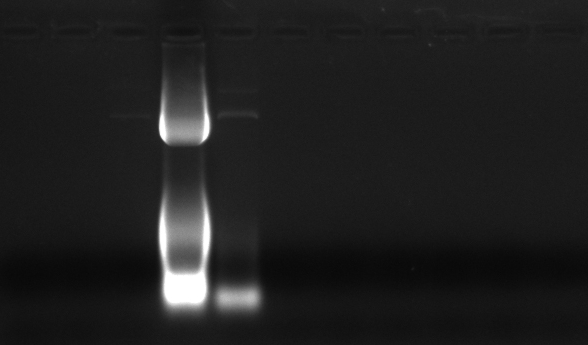
\includegraphics[width=6.3cm]{ef_s100.jpg}};

\node[white, above, font = \normalsize] at (5.400, 2) { 1};
\node[white, above, font = \normalsize] at (6.000, 2) { 2};
\node[white, above, font = \normalsize] at (6.600, 2) { 3};
\node[white, above, font = \normalsize] at (7.200, 2) { 4};
\node[white, above, font = \normalsize] at (7.850, 2) { 5};
\node[white, above, font = \normalsize] at (8.475, 2) { 6};
\node[white, above, font = \normalsize] at (9.150, 2) { 7};
\node[white, above, font = \normalsize] at (9.750, 2) { 8};
\node[white, above, font = \normalsize] at (10.35, 2) { 9};
\node[white, above, font = \normalsize] at (11.00, 2) {10};
\node[white, above, font = \normalsize] at (11.70, 2) {11};

\end{tikzpicture}
    \caption[Análise do lisado centrifugado com o gel Sephacryl S-100.]{Análise do lisado centrifugado obtido após lise alcalina de \ecoli\ contendo o plasmídeo \pVAX. a) Perfil cromatográfico do lisado no gel Sephacryl S-100 HF (SEC). No mesmo gráfico encontram-se sobrepostos os valores de concentração de proteína total, obtidos para cada fração recolhida; b) Análise por HIC-HPLC das frações 4, 5, e 8, recolhidas durante o ensaio de SEC. c) Análise por eletroforese das frações recolhidas durante o ensaio de SEC.}
    \label{fig:s100}
\end{figure}

A análise feita permite assim concluir uma importante característica do método de HIC face à caracterização de lisados, nomeadamente a possibilidade de quantificar numa só análise quer o pDNA (região 1) quer o RNA total presente (região 3). Os compostos que absorvem na região 2 apresentam uma menor massa molecular, sendo maioritariamente detetado nesta zona o material proteico presente nos lisados. Apesar de não serem aqui discutidos, os lisados do plasmídeo \pCAMBIA\ (usados no capítulo~\ref{chap:art4}) apresentam resultados semelhantes. Espera-se que o material proteico presente nos lisados, pelo facto de apresentar uma menor massa molecular, possa ser separado do pDNA através de uma operação de ultrafiltração, tendo este resultado sido já verificado na prática \cite{duvaltff,freitas}.  


\cleardoublepage
\cleardoublepage

\printindex

\end{document}
